% arara: pdflatex: { synctex: on } 
% arara: makeindex 
% arara: pdflatex: { synctex: on } 

\newcommand{\version}{0.99}

% This file was initially converted to LaTeX by Writer2LaTeX ver. 1.1.8
% (see http://writer2latex.sourceforge.net for more info)
% 
% Further formatting was done using the isov2 LaTeX package

%% Global switches
%% Do we pretend that this is a final version?
\newif\ifpretendfinal
\pretendfinalfalse 
%% Real PDF comments, or "paper" margin notes (using todonotes package)?
%%\newif\ifpdfcomment
%%\pdfcommenttrue
%%\pdfcommentfalse


%\documentclass[10pt, a4paper]{isov2} 
%\documentclass[10pt, letterpaper]{isov2} 
\documentclass[10pt, a4paper]{isov2} 

%% Cleaning up things that isov2 gets wrong
\makeatletter
%% Other packages define a more modern variant of \ifpdf
\let\ifpdf\@undefined
%% Need to use the mathematical \begin{definition}
\end{definition} environment; that's incompatible with \definition from isov2; therefore we rename the latter
\let\termdefinition\definition
\let\definition\@undefined
%% manipulate the section counter, so that AMS-style theorems work
\def\c@section{0}
\makeatother


% % In isov2 the footer is reserved for the copyrightstatement.
% % OMG wants a footer, so we just overwrite the iso copyright for that purpose.
% \newcommand{\DOLfooter}[0]{
% \renewcommand{\copyrighthead}{\mbox{\scriptsize{\textsf{Distributed Ontology, Model, and Specification Language (DOL), v1.0 Beta}}}}
% 	}
% \newcommand{\onlypagenumberfooter}[0]{
% \renewcommand{\copyrighthead}{\mbox{}}
% 	}
%
%




\textwidth 17.5cm
\hoffset -0.7cm
\textheight 24cm
%\voffset 1cm


\setcounter{secnumdepth}{4}
\setcounter{tocdepth}{4}
\def\toclevel@subsubsection{4}

\usepackage{isobib} 
\usepackage{pdflscape}


\usepackage{fancyhdr}
\pagestyle{fancy}
%\fancyhead[LO,RE]{}
%\fancyhead[RO,LE]{}
\fancyfoot[LO,RE]{\iffloatpage{}{\scriptsize{\textsf{Distributed Ontology, Model, and Specification Language (DOL), v1.0 Beta}}}}
\fancyfoot[RO,LE]{\iffloatpage{\thepage}{\thepage}}
\renewcommand{\headrulewidth}{0pt}
\renewcommand{\footrulewidth}{0pt}
%\renewcommand{\headrulewidth}{\iffloatpage{0pt}{0.4pt}}


\usepackage{multicol}


%%\usepackage[show]{ed}
\usepackage[hide]{ed}

%%color highlight, for editing
\usepackage{color}
\newcommand{\red}[1]{#1} %{\color{red}{#1}}} % currently, no color highlighting

%% Hacks
%%\usepackage{savesym}

%% Font and language
\usepackage[utf8]{inputenc}
\usepackage[T1]{fontenc}
\usepackage[english]{babel}
\usepackage{textcomp}

\renewcommand{\ttdefault}{pcr} % Select courier as default tt-fontstyle because Computer Modern has no bold font implemented

%%\usepackage{lmodern} % FN: commented out since OMG wants its own fonts
%%\usepackage[scaled=.8]{beramono} % FN: commented out since OMG wants its own fonts
%\usepackage{courier}
%\usepackage[scaled=.9]{helvet}



%%\usepackage{lmodern} %DIF > 
%%\usepackage[scaled=.8]{beramono} %DIF > 
%% set up Unicode symbols
\DeclareUnicodeCharacter{21A6}{\ensuremath{\mapsto}}

%% Keyword Index 
\usepackage{makeidx}
\makeindex

%% used in definition of \termref, \termdefinition  
\newcommand{\dolindex}{Distributed Ontology Modeling and Specification Language (DOL)}

%% Math
%% \usepackage{mathtools}
%% reintroducing a math-style \begin{definition}...\end{definition} environment %DIF > 

%% \usepackage{amsthm}
%% \theoremstyle{definition}
%% \newtheorem{definition}{Definition}
\usepackage{hetonto-subset}
%% \usepackage{diagrams}

%% section titles

\usepackage{titlesec}

\titleformat{name=\clause}
  {\normalfont\Large\bfseries}{\theclause}{2em}{\hspace{-1em}}{}
\titleformat{name=\clause,numberless}
  {\normalfont\Large\bfseries}{}{1em}{\hspace{-1em}}{}
\titleformat{name=\sclause}
  {\normalfont\large\bfseries}{\thesclause}{2em}{\hspace{-1em}}{}
\titleformat{name=\sclause,numberless}
  {\normalfont\large\bfseries}{}{1em}{\hspace{-1em}}{}
\titleformat{name=\ssclause}
  {\normalfont\bfseries}{\thessclause}{2em}{\hspace{-1em}}{}
\titleformat{name=\ssclause,numberless}
  {\normalfont\bfseries}{}{1em}{\hspace{-1em}}{}
\titleformat{name=\sssclause}
  {\normalfont\bfseries}{\thesssclause}{2em}{\hspace{-1em}}{}
\titleformat{name=\sssclause,numberless}
  {\normalfont\bfseries}{}{1em}{\hspace{-1em}}{}

%% Utilities
\usepackage{etoolbox}
\usepackage{ifmtarg}
\usepackage{stringstrings}
\usepackage{stmaryrd}
\usepackage[inline]{enumitem}
\usepackage{setspace}

%% Graphics
\usepackage{standalone}
\usepackage[pdftex]{graphicx}
\usepackage{tikz}
\usepackage{rotating}
\usetikzlibrary{matrix,shapes,arrows,calc}
\usepackage{tikz-uml}
\usetikzlibrary{shadows,shapes,positioning,arrows}
\tikzstyle{ontoiop}=[font=\sffamily,
    language/.style={circle,draw},
    translation/.style={-stealth'},
    dol/.style={rectangle,rounded corners,draw,align=left},
    import/.style={-o},
]
% Our colors
\definecolor{cl}{RGB}{127,129,209}
\definecolor{owl}{RGB}{138,173,72}
\definecolor{rdfs}{RGB}{232,146,31}
\definecolor{dol}{RGB}{253,246,234}
\definecolor{owlxml}{RGB}{240,251,239}
\definecolor{clif}{RGB}{242,242,251}




%% Content
\usepackage{ctable}
\usepackage[final]{listings}
\lstset{basicstyle=\ttfamily\small,columns=fixed}
\usepackage{lstsemantic}
\usepackage{algorithmic}


%% linguistics
\usepackage{xspace}
%% English
\newcommand*{\cf}{cf.\@\xspace}
\newcommand*{\eg}{e.g.\@\xspace}
\newcommand*{\etal}{et al.\@\xspace}
\newcommand*{\ie}{i.e.\@\xspace}
\newcommand*{\vs}{vs.\@\xspace}
\newcommand*{\wrt}{w.r.t.\@\xspace}
%% Quotes
\usepackage[babel]{csquotes}
%%\MakeAutoQuote{“}{”}
%%\MakeAutoQuote*{‘}{’}
\MakeAutoQuote{“}{”}
\MakeAutoQuote*{‘}{’}

%% Hyperref
\usepackage[
          %% we want hyperlinks even in draft mode
          final,
          plainpages=false,
          pdfpagelabels,
          bookmarksnumbered,
          hyperindex=true
         ]{hyperref}

%% To-do notes and/or comments
%% \savesymbol{todo}
%% \restoresymbol{ed}{todo}

\usepackage{xkeyval}
\makeatletter
%% author
\newcommand*\CommentAuthor{}
\define@key{Comment}{author}{%
\renewcommand*\CommentAuthor{#1}}
%% date
\newcommand*\CommentDate{}
\define@key{Comment}{date}{%
\renewcommand*\CommentDate{#1}}
%% id
\newcommand*\CommentId{}
\define@key{Comment}{id}{%
\renewcommand*\CommentId{#1}}
%% replyto
\newcommand*\CommentReplyTo{}
\define@key{Comment}{replyto}{%
\renewcommand*\CommentReplyTo{#1}}
%% type (currently represented as color and text prefix)
\newcommand*\CommentType{}
\define@key{Comment}{type}{%
\renewcommand*\CommentType{#1}}
\makeatother
\presetkeys{Comment}{%
author=,date=,id=,replyto=,type=}{}%

\newcommand*{\SetCommentColorByType}[1]{%
%% http://tex.stackexchange.com/questions/24922/comparing-an-argument-to-a-string-when-argument-is-a-result-of-a-command-with-et
\edef\localType{{#1}}% enforce expansion of #1
\expandafter\ifstrequal\localType{q-aut}{\colorlet{CommentColor}{red}}{%
\expandafter\ifstrequal\localType{q-all}{\colorlet{CommentColor}{orange}}{%
\expandafter\ifstrequal\localType{todo}{\colorlet{CommentColor}{orange}}{%
\expandafter\ifstrequal\localType{fyi}{\colorlet{CommentColor}{lightgray}}{%
\colorlet{CommentColor}{yellow}}}}}}
\makeatletter
\newcommand*{\SetCommentPrefixByType}[1]{%
\edef\localType{{#1}}% enforce expansion of #1
\expandafter\@ifmtarg\localType{% if empty
\edef\CommentPrefix{}%
}{% if not empty
\caseupper[q]{#1}%
\edef\CommentPrefix{\thestring: }%
}}
\makeatother

\newcommand*{\initComment}[1]{%
\setkeys{Comment}{#1}%
\SetCommentColorByType{\CommentType}%
\relax%
\SetCommentPrefixByType{\CommentType}%
\relax%
}

\makeatletter
%%\ifpdfcomment
%% forward class options "draft" or "final" into document
\ifdr@ftd@c
\usepackage[draft]{pdfcomment}
\else
\usepackage[final]{pdfcomment}
\fi


\newcommand*{\todonote}[2][]{%
\initComment{#1}%
\pdfcomment[author=\CommentAuthor,color=CommentColor,date=\CommentDate,id=\CommentId]{%
\CommentPrefix
%%\usebox{CommentPrefix}
#2}}


\newcommand*{\reply}[2][]{%
\initComment{#1}%
\pdfreply[author=\CommentAuthor,color=CommentColor,date=\CommentDate,id=\CommentId,replyto=\CommentReplyTo]{%
%%\usebox{CommentPrefix}
#2}}

\newcommand*{\markupcomment}[3][]{%
\initComment{#1}%
\pdfmarkupcomment[author=\CommentAuthor,color=CommentColor,date=\CommentDate,id=\CommentId]{#2}{%
%%\usebox{CommentPrefix}
#3}}

%% Hyperlinks don't work inside pdfcomment's PDF comments :-(
\newcommand*{\todonoteURL}[1]{#1}


%%\else % \ifpdfcomment 
%%\ifdr@ftd@c  
%%\usepackage[show]{ed} 
%%\else  
%%\usepackage[hide]{ed} 
%%\fi 
%% \usepackage[obeyDraft,textsize=tiny]{todonotes} % must load after tikz


%%FN I commented the above out, because I could not get it to work, instead I include

\renewcommand*{\todonote}[2][]{% FN: Changed newcommand to renewcommand
%%\newcommand*{\todonote}[2][]{% %DIF > 
\initComment{#1}%
%% TODO set color according to type
%% TODO display author (unless empty)
%% TODO display date (unless empty)
\ednote{\CommentPrefix #2}}


\renewcommand*{\reply}[2][]{% FN: Changed newcommand to renewcommand
%%\newcommand*{\reply}[2][]{% %DIF > 
\initComment{#1}%
%% TODO set color according to type
%% TODO display author (unless empty)
%% TODO display date (unless empty)
\ednote{Reply: \CommentPrefix #2}}


\renewcommand*{\markupcomment}[3][]{% FN: Changed newcommand to renewcommand
%%\newcommand*{\markupcomment}[3][]{% %DIF > 
\initComment{#1}%
%% TODO set color according to type
%% TODO display author (unless empty)
%% TODO display date (unless empty)
\ednote{\CommentPrefix #3}#2}

%% dummy versions of some pdfcomment commands
\renewcommand*{\textLF}{\\}


\renewcommand*{\todonoteURL}[1]{\url{#1}} %DIF > 
%%\fi % \ifpdfcomment %DIF > 

\makeatother
\newcommand*{\ticket}[1]{\todonoteURL{http://trac.informatik.uni-bremen.de:8080/OntoIOp/ticket/#1}}

%% comment commands for frequent users
\newcommand*{\CLnote}[2][author=Christoph Lange]{%
\todonote[author=Christoph Lange,#1]{#2}}

\newcommand{\toleft}{\noindent$x\!\!\!\!\!\!\!\!\!\!\!\!\!\!\!\!\!\!\!\!\!\!\!\!\!\!\!\!\!\!\!\!\!\!\!\!\!\!\!\!\!\!\!\!\!\!\!\!\!\!\!\!\!\!\!\!\!\!\!\!\!\!\!\!\!$}
\newcommand*{\lessthan}{<}
\newcommand*{\greaterthan}{>}


%% ISO structures not defined by isov2.cls, and additional semantic macros
%% cross-reference to a normative reference
\newcommand*{\nitem}[1]{[#1]}

%%\newcommand*{\nisref}[1]{[#1]} %DIF > 

%% reference from the definition of one term to another defined term
\newcommand*{\termref}[1]{\index{#1}#1\xspace}
%%\newcommand*{\termref}[1]{\textit{#1}} %DIF > 
%% subject field restriction of a term
\newcommand*{\subjectfield}[1]{ {\textlangle}#1{\textrangle}}
%% synonym of a term

\newcommand*{\synonym}{\\} %DIF > 
\newcommand*{\mimetype}[1]{\textit{#1}}
\newcommand*{\institutionsOnly}{\bfseries\itshape}
\newcommand*{\syntax}[1]{\texttt{#1}}

%% requirements (as per Annex H of ISO/IEC Directives, Part 2)
\newcommand*{\notallowed}{\textbf{not allowed}\xspace}
\newcommand*{\notrequired}{\textbf{not required}\xspace}
\newcommand*{\required}{\textbf{required}\xspace}
\newcommand*{\recommended}{\textbf{recommended}\xspace}
\newcommand*{\shallnot}{\textbf{shall not}\xspace}
\newcommand*{\shall}{\textbf{shall}\xspace}
\newcommand*{\shouldnot}{\textbf{should not}\xspace}
\newcommand*{\should}{\textbf{should}\xspace}
\newcommand*{\may}{\textbf{may}\xspace}
\newcommand*{\hasto}{\textbf{must}\xspace}

%%\newcommand*{\hasto}{\textbf{has to}\xspace} %DIF > 


%% abbreviations
\newcommand*{\IS}{OMG Specification\xspace}

%%\newcommand*{\IS}{OMG Standard\xspace} %DIF > 


%% Math macros
%%\newcommand{\Mod}{\ensuremath{\mathrm{Mod}}}
%%\newcommand{\Sen}{\ensuremath{\mathrm{Sen}}}
%%\newcommand{\Sign}{\ensuremath{\mathrm{Sign}}}
\newcommand{\conjclause}{\ensuremath{p_1 \wedge \dots \wedge p_n}}
\newcommand{\id}{\ensuremath{\operatorname{id}}}
\newcommand{\powerset}[1]{\mathcal{P}(#1)}
\newcommand{\finorderedpowerset}{\mathcal{P}^{\mathrm{ord}}_{\mathrm{fin}}}
\newcommand{\finpowerset}{\mathcal{P}_{\mathrm{fin}}}
\newcommand{\reductop}{\mathnormal{|}}

%% from HetCASL summary
\newcommand{\Si}{\Sigma}
\newcommand{\al}{\alpha}
\newcommand{\ModFunctor}{\mathbf{Mod}}
\newcommand{\SenFunctor}{\mathbf{Sen}}
\newcommand{\Sig}{\mathsf{Sig}}
\renewcommand{\Th}{\mathsf{Th}}
\newcommand{\Mor}{\mathsf{Mor}}
%%\newcommand{\Sig}{\mathbf{Sig}} %DIF > 
\newcommand{\PF}{\mathit{PF}}
\newcommand{\TF}{\mathit{TF}}

\newcommand{\Inst}{\ensuremath{\mathbf{Inst}}}
\newcommand{\Name}{\ensuremath{\mathbf{Name}}}
%\newcommand{\map}[2]{\colon#1\!\longrightarrow\!#2}

\newcommand{\Gram}[1]{\texttt{#1}}
\newcommand{\Gx}[1]{\texttt{#1}}

\newenvironment{Grammar}
 {%\texonly{\footnotesize}
  \begin{example}}{\end{example}\ignorespaces}

\newenvironment{AbstractGrammar}
 {\par%\texonly{\smallskip\samepage}
   \begin{Grammar}}{\end{Grammar}\par}

\newenvironment{ConcreteDisplay}
 {\nopagebreak\begin{quote}\casl}{\end{quote}\pagebreak[3]}

\newenvironment{ConcreteInput}
 {\begin{example}}{\end{example}\ignorespaces}

\newcommand{\DisplayLatexInput}[3]
 {The sign displayed as 
 \texorhtml{`\begin{casl}\(#1\)\end{casl}'}{#2 in \LaTeX}
 is input as `\Gram{#3}'.} 

\newcommand{\DisplayISOInput}[3]
 {The sign displayed as `\begin{casl}\(#1\)\end{casl}' may be input as
 `\math{#2}' in ISO Latin-1, or as `\Gram{#3}' in ASCII.} 

\newcommand*{\CL}{\ensuremath{\mathsf{CL}}\xspace}
\newcommand{\QL}{\ensuremath{\mathsf{QL}}\xspace}
\newcommand{\RL}{\ensuremath{\mathsf{RL}}\xspace}
\newcommand{\EL}{\ensuremath{\mathsf{EL}}\xspace}

\newcommand*{\meta}{\ensuremath{\operatorname{meta}}\xspace}

\newcommand{\BASICOMS}{\ensuremath{\langle\Sigma,\Delta\rangle}\xspace}
%%\newcommand{\BASICONTO}{\ensuremath{\langle\Sigma,\Delta\rangle}\xspace} %DIF > 


\newcommand{\semdom}[1]{
\begin{center}
\fbox{$#1$}
\end{center}
}

\newcommand{\mBox}[1]{\, \mbox{#1} \,}
\newcommand{\twocase}[3]{
\left\{
\begin{array}{ll}
  #1,&\mBox{if }#2\\
  #3,&\mBox{otherwise}
\end{array}\right.}

\newcommand{\threecase}[5]{
\left\{
\begin{array}{ll}
  #1,&\mBox{if }#2\\
  #3,&\mBox{if }#4\\
  #5,&\mBox{otherwise}
\end{array}\right.}

%% Logics
\newcommand{\ELDL}{\ensuremath{\mathcal{EL}}\xspace}
\newcommand*{\DOL}{\ensuremath{\mathsf{DOL}}\xspace}
\newcommand*{\PL}{\ensuremath{\mathit{PL}}\xspace}
\newcommand{\CLminus}{\ensuremath{{\CL}^{-}}\xspace} 

%% translations
\newcommand{\translate}[2]{\ensuremath{{#1}{\to}{#2}}\xspace}
\newcommand{\PropToOWL}{\translate\Prop\OWL}
\newcommand{\PropToFOL}{\translate\Prop\FOL}
\newcommand{\ELToOWL}{\translate\EL\OWL}
\newcommand{\OWLToFOL}{\translate\OWL\FOL}
\newcommand{\OWLToCL}{\translate\OWL\CL}
\newcommand{\FOLToCL}{\translate\FOL\CL}

\newcommand{\holds}[1]{\ensuremath\mathtt{Holds}_{#1}\xspace}
\newcommand{\apply}[1]{\ensuremath\mathtt{App}_{#1}\xspace}
%% renewing the command since it is already part of isov2 style
%\renewcommand{\outofscopename}{The following are outside the scope of this }
%\renewcommand{\pagename}{Page}
%\renewcommand{\tbpname}{To be published.}
\renewcommand{\annexrefname}{annex}
\renewcommand{\clauserefname}{clause}
\renewcommand{\examplerefname}{example}
\renewcommand{\figurerefname}{Figure}
\renewcommand{\noterefname}{note}
\renewcommand{\tablerefname}{Table}
\renewcommand{\pagerefname}{page}
\renewcommand{\refname}{}
%\renewcommand{\isourl}[1]{\texttt{<}\url{#1}\texttt{>}}
\renewcommand{\aref}[1]{\annexrefname~\ref{#1}}
%\renewcommand{\bref}[1]{\cite{#1}}
\renewcommand{\cref}[1]{\clauserefname~\ref{#1}}
\renewcommand{\eref}[1]{\examplerefname~\ref{#1}}
\renewcommand{\fref}[1]{\figurerefname~\ref{#1}}
\renewcommand{\nref}[1]{\noterefname~\ref{#1}}
\renewcommand{\tref}[1]{\tablerefname~\ref{#1}}
\renewcommand{\pref}[1]{\pagerefname~\pageref{#1}}
\newcommand{\rtm}[0]{\small{\textregistered\xspace}}
\newcommand{\OMGparagraph}[1]{
\vspace{23pt}
%\bigskip
{\centerline {#1}}
\vspace{3pt}
}

\usepackage{xparse}
%\newlength{\currentindent}
% \newsavebox{\fminipagebox}
% \setlength{\currentindent}{\parindent}
% \NewDocumentEnvironment{fminipage}{m O{\fboxsep}}
%   {
%   \par\kern#2\noindent\begin{lrbox}{\fminipagebox}
%   \begin{minipage}{#1}\ignorespaces  \setlength{\parindent}{\currentindent}}
%   {\end{minipage}\end{lrbox}%
%    \makebox[#1]{%
%     \kern\dimexpr-\fboxsep-\fboxrule\relax
%       \fbox{\usebox{\fminipagebox}}%
%       \kern\dimexpr-\fboxsep-\fboxrule\relax
%     }\par\kern#2
%    }
%

\usepackage{mdframed}




\renewenvironment{symbols}[0]{\begin{longtable}{p{.15\textwidth}p{.84\textwidth}}}{\end{longtable}}
\renewcommand{\symboldef}[2]{ #1 & #2 \\}


\usepackage{textcomp}
\usepackage{longtable}
\newcommand{\normative}[0]{{\begin{center}{\Large{(Normative})}\end{center}} \bigskip}
\newcommand{\informative}[0]{{\begin{center}{\Large{(Informative})}\end{center}} \bigskip}

%\newcommand{\sectionWN}[1]{\sclause{#1}\addcontentsline{toc}{section}{#1}} 


\newcommand{\prefix}{\mathit{prefix}}
\newcommand{\current}{\mathit{current}}
\newcommand{\PMap}{\mathit{PMap}}
% Temporary Hacks (to be removed later or cleaned up) 

\renewcommand{\nref}[1]{\ref{nref-#1}}
%% Commented out to remove the redundancy. and wrong use of \chapter command, since \chapter command is not part of isov2.

%\renewcommand{\clause}[1]{\chapter{#1}}
%\newcommand{\clauseN}[1]{\chapter{#1} \normative}
\newcommand{\clauseI}[1]{\clause{#1} \informative}
%\renewcommand{\sclause}[1]{\section{#1}}
%\renewcommand{\ssclause}[1]{\subsection{#1}}
%\renewcommand{\sssclause}[1]{\subsubsection{#1}}
\renewcommand{\termdefinition}[2]{\index{#1}\textbf{#1} #2}
%\newcommand{\termdefinitionLight}[2]{\paragraph{#1} #2}
\newcommand{\termdefinitionLight}[2]{\textbf{#1} #2}
\newcommand{\nisref}[1]{#1}
\renewcommand{\subjectfield}[1]{} % {#1}
%\renewcommand{\normannex}[1]{ \sclause{Annex: #1} \normative}
%\renewcommand{\infannex}[1]{\sclause{Annex: #1}  \informative }
\renewenvironment{definitions}[0]{\medskip }{}
\renewenvironment{note}[0]{\ \\ \textsc{Note} \quad}{}
\renewenvironment{example}[0]{\ \newline \textsc{Example}\quad }{}



\usepackage{afterpage}

\newcommand\blankpage{%
      \null
      \thispagestyle{empty}%
      \addtocounter{page}{-1}%
      \newpage}

\newcommand{\uml}[1]{\textsf{#1}}
\newcommand{\stereotype}[1]{\uml{\flqq#1\frqq}}
\newcommand{\aggregation}{\raisebox{0.2pt}{\begin{sideways}\fontsize{6pt}{6pt}\selectfont$\lozenge$\end{sideways}}}
\newcommand{\composition}{\raisebox{0.2pt}{\begin{sideways}\fontsize{6pt}{6pt}\selectfont$\blacklozenge$\end{sideways}}}
\newcommand{\Tau}{\mathrm{T}}
\newcommand{\NZ}{\mathbb{Z}}
\newcommand{\ZZ}{\mathbb{Z}}
\newcommand{\sem}[1]{\mathopen\llbracket#1\mathclose\rrbracket}
\newcommand{\white}[1]{{\color{white}{#1}}}
\newcommand{\qqquad}{\white{x}\qquad}


\allowdisplaybreaks



\begin{document}

\nocite{OM2014,JYB-Festschrift2015-DOL,womo13,DOL-TKE2012,DOL-3semantics,blendingc3gi12,hyper2010}


\pagestyle{headings}  %%% switches on printing of running heads


\begin{flushright}
  \textbf{Date:} January 2016 
\end{flushright}

\begin{flushleft}
  \begin{figure}[h]
    
\includegraphics[width=196pt]{OMG-logo-2015.pdf}
 \end{figure}
 
\bigskip\bigskip

\bigskip\bigskip

\bigskip
\textsf{\fontsize{20}{20}\selectfont{}The Distributed Ontology, Modeling, and Specification Language (DOL)}


\bigskip

\textsf{\textit{\fontsize{16}{16}\selectfont{}FTF -- Beta}}
%Version \version %DIFDELCMD < 


\bigskip\bigskip\bigskip



\vskip\medskipamount %%% or other desired dimension
\leaders\vrule width \textwidth\vskip1pt %%% or other desired thickness
\vskip 6pt 
\nointerlineskip
\begin{onehalfspace}
\textsf{\textbf{OMG Document Number:}}    \\  %ad/2015-08-01 ad/2015-05-03 ad/15-06-04
\textsf{\textbf{Standard document URL: \ \url{http://www.omg.org/spec/DOL/1.0/PDF}}} \\
\textsf{\textbf{Machine Consumable File(s): \\ 
\leftskip2em Normative:  \\
\url{http://www.omg.org/spec/DOL/20151109/DOL-metamodel.xmi}\\
Informative: \\
\url{http://www.omg.org/spec/DOL/20151109/DOL-terms.rdf} \\}}
\end{onehalfspace} 

\vskip 28pt
\leaders\vrule width \textwidth\vskip1pt % or other desired thickness
\vskip\medskipamount % ditto
\nointerlineskip

This OMG document replaces the submission document (ad/2015-10-01). It is an OMG Adopted Beta specification and is currently in the finalization phase. Comments on the content of this document are welcome, and should be directed to \url{issues@omg.org} by March 28, 2016. 

You may view the pending issues for this specification from the OMG revision issues web page %http://www.omg.org/issues/
\url{http://issues.omg.org/browse/DOL}.

The FTF Recommendation and Report for this specification will be published on September 23, 2016. If you are reading this after that date, please download the available specification from the OMG Specifications Catalog.

\end{flushleft}



\pagenumbering{gobble}% Remove page numbers (and reset to 1)
\thispagestyle{empty}
\clearpage

\pagenumbering{roman} 
  

\noindent Copyright \copyright 2014-15, Object Management Group, Inc.\\
Copyright \copyright 2014-15, Fraunhofer FOKUS\\
Copyright \copyright 2014-15, MITRE\\
Copyright \copyright 2014-15, Otto-von-Guericke-Universit{\"a}t Magdeburg  \\
Copyright \copyright 2014-15, Thematix Partners LLC \\
Copyright \copyright 2014-15, Athan Services \\



\OMGparagraph{USE OF SPECIFICATION - TERMS, CONDITIONS \& NOTICES}
The material in this document details an Object Management Group specification in accordance with
 the terms, conditions and notices set forth below. This document does not represent a commitment
  to implement any portion of this specification in any company's products. The information
   contained in this document is subject to change without notice.


\OMGparagraph{LICENSES}
The companies listed above have granted to the Object Management Group, Inc. (OMG) a nonexclusive,
 royalty-free, paid up, worldwide license to copy and distribute this document and to modify this 
  document and distribute copies of the modified version. Each of the copyright holders listed 
   above has agreed that no person shall be deemed to have infringed the copyright in the included 
    material of any such copyright holder by reason of having used the specification set forth 
	 herein or having conformed any computer software to the specification.

Subject to all of the terms and conditions below, the owners of the copyright in this specification 
hereby grant you a fully-paid up, non-exclusive, nontransferable, perpetual, worldwide license 
 (without the right to sublicense), to use this specification to create and distribute software and 
  special purpose specifications that are based upon this specification, and to use, copy, and 
distribute this specification as provided under the Copyright Act; provided that: (1) both the 
 copyright notice identified above and this permission notice appear on any copies of this 
  specification; (2) the use of the specifications is for informational purposes and will not be 
copied or posted on any network computer or broadcast in any media and will not be otherwise resold 
 or transferred for commercial purposes; and (3) no modifications are made to this specification. 
This limited permission automatically terminates without notice if you breach any of these terms or 
 conditions. Upon termination, you will destroy immediately any copies of the specifications in 
  your possession or control.



\OMGparagraph{PATENTS}
The attention of adopters is directed to the possibility that compliance with or adoption of OMG 
 specifications may require use of an invention covered by patent rights. OMG shall not be 
  responsible for identifying patents for which a license may be required by any OMG specification, 
   or for conducting legal inquiries into the legal validity or scope of those patents that are 
    brought to its attention. OMG specifications are prospective and advisory only. Prospective 
	 users are responsible for protecting themselves against liability for infringement of patents.

\OMGparagraph{GENERAL USE RESTRICTIONS}
Any unauthorized use of this specification may violate copyright laws, trademark laws, and 
 communications regulations and statutes. This document contains information which is protected by 
  copyright. All Rights Reserved. No part of this work covered by copyright herein may be 
   reproduced or used in any form or by any means--graphic, electronic, or mechanical, including 
    photocopying, recording, taping, or information storage and retrieval systems--without 
	 permission of the copyright owner.

\newpage
\OMGparagraph{DISCLAIMER OF WARRANTY}
WHILE THIS PUBLICATION IS BELIEVED TO BE ACCURATE, IT IS PROVIDED "AS IS" AND MAY CONTAIN ERRORS OR MISPRINTS. THE OBJECT MANAGEMENT GROUP AND THE COMPANIES LISTED ABOVE MAKE NO WARRANTY OF ANY KIND, EXPRESS OR IMPLIED, WITH REGARD TO THIS PUBLICATION, INCLUDING BUT NOT LIMITED TO ANY WARRANTY OF TITLE OR OWNERSHIP, IMPLIED WARRANTY OF MERCHANTABILITY OR WARRANTY OF FITNESS FOR A PARTICULAR PURPOSE OR USE. IN NO EVENT SHALL THE OBJECT MANAGEMENT GROUP OR ANY OF THE COMPANIES LISTED ABOVE BE LIABLE FOR ERRORS CONTAINED HEREIN OR FOR DIRECT, INDIRECT, INCIDENTAL, SPECIAL, CONSEQUENTIAL, RELIANCE OR COVER DAMAGES, INCLUDING LOSS OF PROFITS, REVENUE, DATA OR USE, INCURRED BY ANY USER OR ANY THIRD PARTY IN CONNECTION WITH THE FURNISHING, PERFORMANCE, OR USE OF THIS MATERIAL, EVEN IF ADVISED OF THE POSSIBILITY OF SUCH DAMAGES.


The entire risk as to the quality and performance of software developed using this specification is borne by you. This disclaimer of warranty constitutes an essential part of the license granted to you to use this specification.


\OMGparagraph{RESTRICTED RIGHTS LEGEND}
Use, duplication or disclosure by the U.S. Government is subject to the restrictions set forth in 
 subparagraph (c) (1) (ii) of The Rights in Technical Data and Computer Software Clause at DFARS 
  252.227-7013 or in subparagraph (c)(1) and (2) of the Commercial Computer Software - Restricted 
   Rights clauses at 48 C.F.R. 52.227-19 or as specified in 48 C.F.R. 227-7202-2 of the DoD F.A.R. 
    Supplement and its successors, or as specified in 48 C.F.R. 12.212 of the Federal Acquisition 
 Regulations and its successors, as applicable. The specification copyright owners are as 
 indicated above and may be contacted through the Object Management Group, 109 Highland 
 Avenue, Needham, MA 02494, U.S.A.
  


\OMGparagraph{TRADEMARKS}

C\rtm, CORBA\rtm, CORBA logos\rtm, FIBO\rtm, Financial Industry Business Ontology\rtm, FINANCIAL INSTRUMENT GLOBAL IDENTIFIER\rtm,  IIOP\rtm, IMM\rtm, Model Driven Architecture\rtm, MDA\rtm, Object Management Group\rtm, OMG\rtm, OMG Logo\rtm, SoaML\rtm, SOAML\rtm, SysML\rtm, UAF\rtm, Unified Modeling Language\rtm, UML\rtm, UML Cube logo\rtm, VSIPL\rtm, and XMI\rtm are registered trademarks of the Object Management Group, Inc. 

For a complete list of trademarks, see: \url{http://www.omg.org/legal/tm_list.htm}. All other products or company names mentioned are used for identification purposes only, and may be trademarks of their respective owners.

\OMGparagraph{COMPLIANCE}
The copyright holders listed above acknowledge that the Object Management Group (acting itself or through its designees) is and shall at all times be the sole entity that may authorize developers, suppliers and sellers of computer software to use certification marks, trademarks or other special designations to indicate compliance with these materials.
Software developed under the terms of this license may claim compliance or conformance with this specification if and only if the software compliance is of a nature fully matching the applicable compliance points as stated in the specification. Software developed only partially matching the applicable compliance points may claim only that the software was based on this specification, but may not claim compliance or conformance with this specification. In the event that testing suites are implemented or approved by Object Management Group, Inc., software developed using this specification may claim compliance or conformance with the specification only if the software satisfactorily completes the testing suites.



\newpage 
\OMGparagraph{OMG's Issue Reporting }
All OMG specifications are subject to continuous review and improvement. As part of this process we encourage readers to report any ambiguities, inconsistencies, or inaccuracies they may find by completing the Issue Reporting Form listed on the main web page \url{http://www.omg.org}, under Documents, Report a Bug/Issue. % \newline(\url{http://www.omg.org/report_issue.htm})

% \newpage
% $ $
% \newpage

\cleardoublepage


\renewcommand{\contentsname}{Table of Contents}
\tableofcontents

%%%%%%%%%%%%%%%%%%%%%%%%%%%%%%%%%%%%%%%%%%%%%%%%%%%%%%%%%%%%%%%%%%%%%%%%%%%%%%%%%%%%%%%%%%%%%%%%%%%%%%%%%%%%%%%%%%%%%%%%%%%%%%%%%%
%%%%%%%%%%%%%%%%%%%%%%%%%%%%%%%%%%%%%%%%%%%%%%%%%%%%%%%%%%%%%%%%%%%%%%%%%%%%%%%%%%%%%%%%%%%%%%%%%%%%%%%%%%%%%%%%%%%%%%%%%%%%%%%%%%
%%%%%%%%%%%%%%%%%%%%%%%%%%%%%%%%%%%%%%%%%%%%%%%%%%%%%%%%%%%%%%%%%%%%%%%%%%%%%%%%%%%%%%%%%%%%%%%%%%%%%%%%%%%%%%%%%%%%%%%%%%%%%%%%%%

\cleardoublepage
\clause*{Preface}
\addcontentsline{toc}{clause}{Preface}

%%%%%%%%%%%%%%%%%%%%%%%%%%%%%%%%%%%%%%%%%%%%%%%%%%%%%%%%%%%%%%%%%%%%%%%%%%%%%%%%%%%%%%%%%%%%%%%%%%%%%%%%%%%%%%%%%%%%%%%%%%%%%%%%%%
%%%%%%%%%%%%%%%%%%%%%%%%%%%%%%%%%%%%%%%%%%%%%%%%%%%%%%%%%%%%%%%%%%%%%%%%%%%%%%%%%%%%%%%%%%%%%%%%%%%%%%%%%%%%%%%%%%%%%%%%%%%%%%%%%%


\sclause*{OMG}
\addcontentsline{toc}{sclause}{OMG}

Founded in 1989, the Object Management Group, Inc. (OMG) is an open membership, not-for-profit 
computer industry standards consortium that produces and maintains computer industry specifications 
for interoperable, portable, and reusable enterprise applications in distributed, heterogeneous 
environments. Membership includes Information Technology vendors, end users, government agencies, 
 and academia. 
 
OMG member companies write, adopt, and maintain its specifications following a mature, open 
 process. OMG's specifications implement the Model Driven Architecture\textregistered \xspace 
 (MDA\textregistered\xspace), maximizing ROI 
  through a full-lifecycle approach to enterprise integration that covers multiple operating 
   systems, programming languages, middleware and networking infrastructures, and software 
    development environments. OMG's specifications include: UML\textregistered\xspace (Unified Modeling Language\texttrademark\xspace); 
	 CORBA\textregistered\xspace (Common Object Request Broker Architecture); CWM\texttrademark\xspace (Common Warehouse Metamodel); and 
	  industry-specific standards for dozens of vertical markets. 
More information on the OMG is available at \url{http://www.omg.org/}.


%%%%%%%%%%%%%%%%%%%%%%%%%%%%%%%%%%%%%%%%%%%%%%%%%%%%%%%%%%%%%%%%%%%%%%%%%%%%%%%%%%%%%%%%%%%%%%%%%%%%%%%%%%%%%%%%%%%%%%%%%%%%%%%%%%
%%%%%%%%%%%%%%%%%%%%%%%%%%%%%%%%%%%%%%%%%%%%%%%%%%%%%%%%%%%%%%%%%%%%%%%%%%%%%%%%%%%%%%%%%%%%%%%%%%%%%%%%%%%%%%%%%%%%%%%%%%%%%%%%%%


\sclause*{OMG Specifications}
\addcontentsline{toc}{sclause}{OMG Specifications}


As noted, OMG specifications address middleware, modeling and vertical domain frameworks. All OMG Specifications are available from the OMG website at:\newline
\url{http://www.omg.org/spec}

\noindent Specifications are organized by the following categories:
\textbf{
\begin{itemize}[leftmargin=*, label={}, topsep=0pt]
	\item  Business Modeling Specifications
	\item Middleware Specifications
	\begin{itemize}[ label={-}, topsep=0pt,itemsep=-1ex,partopsep=1ex,parsep=1ex]
		\item CORBA/IIOP
		\item Data Distribution Services
		\item Specialized CORBA
	\end{itemize}				
	\item IDL/Language Mapping Specifications
	\item Modeling and Metadata Specifications
	\begin{itemize}[ label={-}, topsep=0pt,itemsep=-1ex,partopsep=1ex,parsep=1ex]	
		\item UML, MOF, CWM, XMI
		\item UML Profile										
	\end{itemize}			
	\item Modernization Specifications
	\item Platform Independent Model (PIM), Platform Specific Model (PSM), Interface Specifications
	\begin{itemize}[ label={-}, topsep=0pt,itemsep=-1ex,partopsep=1ex,parsep=1ex]	
		\item CORBAServices
		\item CORBAFacilities
	\end{itemize}			
	\item OMG Domain Specifications
	\item CORBA Embedded Intelligence Specifications
	\item CORBA Security Specifications
\end{itemize}	
}

\medskip 
\noindent
All of OMG's formal specifications may be downloaded without charge from our website. (Products implementing OMG specifications are available from
 individual suppliers.) Copies of specifications, available in PostScript and
 PDF format, may be obtained from the Specifications Catalog cited above or by contacting the Object Management Group, Inc. at:



\medskip
\noindent 
OMG Headquarters \\
109 Highland Avenue \\
Needham, MA 02494 \\
USA\\
Tel: +1-781-444-0404\\
Fax: +1-781-444-0320\\
Email: \url{pubs@omg.org}\\

\noindent Certain OMG specifications are also available as ISO standards. Please consult \url{http://www.iso.org}.

%%%%%%%%%%%%%%%%%%%%%%%%%%%%%%%%%%%%%%%%%%%%%%%%%%%%%%%%%%%%%%%%%%%%%%%%%%%%%%%%%%%%%%%%%%%%%%%%%%%%%%%%%%%%%%%%%%%%%%%%%%%%%%%%%%
%%%%%%%%%%%%%%%%%%%%%%%%%%%%%%%%%%%%%%%%%%%%%%%%%%%%%%%%%%%%%%%%%%%%%%%%%%%%%%%%%%%%%%%%%%%%%%%%%%%%%%%%%%%%%%%%%%%%%%%%%%%%%%%%%%


\sclause*{Typographical Conventions}
\addcontentsline{toc}{sclause}{Typographical Conventions}

The type styles shown below are used in this document to distinguish
 programming statements from ordinary English. However, these conventions are
 not used in tables or section headings where no distinction is necessary.


% normal text  
% texttt{} fuer code
% bold texttt fuer keywords 
% lstlisting for grammar
\medskip \noindent
Computer Modern Roman: Standard body text

\lstinline{Courier}: DOL code and DOL syntax elements

\lstinline[keywordstyle=\color{black}\bfseries, keywords={Courier, bold}]{Courier bold}: keywords in DOL code



%
% \medskip \noindent
% {\fontencoding{T1}\fontfamily{phv}\fontseries{b}\fontshape{n}\selectfont
% Helvetica/Arial - 10 pt. Bold: } OMG Interface Definition Language (OMG IDL)
% and syntax elements.
%
% \medskip \noindent
% \texttt{\textbf {Courier - 10 pt. Bold:}}  Programming language elements.
%
% \medskip \noindent
% {\fontencoding{T1}\fontfamily{phv}\fontseries{m}\fontshape{n}\selectfont
% Helvetica/Arial - 10 pt.: } Exceptions
%
% \medskip\noindent
% NOTE: Italic text represents names defined in the specification or the name of
%  a document, specification, or other publication.

%%%%%%%%%%%%%%%%%%%%%%%%%%%%%%%%%%%%%%%%%%%%%%%%%%%%%%%%%%%%%%%%%%%%%%%%%%%%%%%%%%%%%%%%%%%%%%%%%%%%%%%%%%%%%%%%%%%%%%%%%%%%%%%%%%
%%%%%%%%%%%%%%%%%%%%%%%%%%%%%%%%%%%%%%%%%%%%%%%%%%%%%%%%%%%%%%%%%%%%%%%%%%%%%%%%%%%%%%%%%%%%%%%%%%%%%%%%%%%%%%%%%%%%%%%%%%%%%%%%%%
 

\sclause*{Issues}
\addcontentsline{toc}{sclause}{Issues}

%%%%%%%%%%%%%%%%%%%%%%%%%%%
The reader is encouraged to report any technical or editing issues/problems
 with this specification by completing the Issue Reporting Form listed on the main web page \url{http://www.omg.org}, under Documents, Report a Bug/Issue.
%%%%%%%%%%%%%%%%%%%%%%%%%%%



%%%%%%%%%%%%%%%%%%%%%%%%%%%%%%%%%%%%%%%%%%%%%%%%%%%%%%%%%%%%%%%%%%%%%%%%%%%%%%%%%%%%%%%%%%%%%%%%%%%%%%%%%%%%%%%%%%%%%%%%%%%%%%%%%%
%%%%%%%%%%%%%%%%%%%%%%%%%%%%%%%%%%%%%%%%%%%%%%%%%%%%%%%%%%%%%%%%%%%%%%%%%%%%%%%%%%%%%%%%%%%%%%%%%%%%%%%%%%%%%%%%%%%%%%%%%%%%%%%%%%
%%%%%%%%%%%%%%%%%%%%%%%%%%%%%%%%%%%%%%%%%%%%%%%%%%%%%%%%%%%%%%%%%%%%%%%%%%%%%%%%%%%%%%%%%%%%%%%%%%%%%%%%%%%%%%%%%%%%%%%%%%%%%%%%%%


%\setcounter{clause}{-1}
\cleardoublepage



\pagestyle{nohead}
\pagestyle{fancy}
\fancyfoot[c]{} % remove default centered page number
\clause{Scope}
\pagenumbering{arabic} 
\sclause{General}
This \IS specifies the Distributed Ontology, Modeling and Specification
 Language (\DOL)\index{\dolindex ! definition}.  \DOL is designed to achieve integration  
and interoperability of
ontologies, specifications and models (OMS for short). \DOL is a language for
distributed knowledge representation, system specification and 
model-driven development across multiple OMS, particularly OMS
 that have been formalized in different OMS languages.
This \IS responds to the
OntoIOp Request for Proposals \cite{RFP}.


%%%%%%%%%%%%%%%%%%%%%%%%%%%%%%%%%%%%%%%%%%%%%%%%%%%%%%%%%%%%%%%%%%%%%%%%%%%%%%%%%%%%%%%%%%%%%%%%%%%%%%%%%%%%%%%%%%%%%%%%%%%%%%%%%%
%%%%%%%%%%%%%%%%%%%%%%%%%%%%%%%%%%%%%%%%%%%%%%%%%%%%%%%%%%%%%%%%%%%%%%%%%%%%%%%%%%%%%%%%%%%%%%%%%%%%%%%%%%%%%%%%%%%%%%%%%%%%%%%%%%


\sclause{Background Information}
Logical languages are used in several fields of computing for the development of formal, 
machine-processable texts that carry a formal semantics. Among those fields are 1) 
\textbf{O}ntologies 
 formalizing domain knowledge, 2) (formal) \textbf{M}odels of systems, and 3) the formal 
\textbf{S}pecification
of systems. Ontologies, models  and specifications will (for the purpose of this document) 
henceforth be abbreviated as \textbf{OMS}\index{OMS}.

An OMS provides formal descriptions, which range in scope from domain knowledge and activities
(ontologies, models) to properties and behaviors of hardware and software systems (models,
specifications). These formal descriptions can be used for the analysis and verification of domain
models, system models and systems themselves, using rigorous and effective reasoning tools.   As 
systems increase in complexity, it becomes concomitantly less practical to provide a monolithic 
logical cover for all.  Instead various models are developed to represent different viewpoints or 
perspectives on a domain or system. 
 Hence, interoperability becomes
a crucial issue, in particular, formal interoperability, i.e.\ interoperability that is based on
the formal semantics of the different viewpoints. Interoperability is both about the ability to 
interface different domains and systems and the ability to use several OMS in a common application
scenario. Further,  interoperability is about coherence and consistency, ensuring at an early stage of the development
that a coherent system can be reached.


In complex applications, which involve multiple OMS with overlapping concept spaces,
it is often necessary to identify correspondences between concepts in the different OMS; this is called  OMS alignment\index{alignment}. 
While OMS alignment is most commonly studied for OMS formalized in the same OMS 
language, the different OMS used by complex applications may also be written in different 
OMS languages, which may even vary in their expressiveness. 
This \IS faces this diversity not by proposing yet another OMS language that would subsume all the others.  
Instead, it accepts the diverse reality and formulates means (on a sound and formal semantic basis) 
to compare and integrate OMS that are written in different formalisms.
It specifies \DOL, a formal language for
expressing not only OMS but also mappings between OMS formalized in different OMS languages.

Thus, \DOL gives interoperability a formal grounding and makes heterogeneous OMS and services based
on them amenable to checking of coherence (\eg consistency, conservativity, intended consequences,
and compliance).


%%%%%%%%%%%%%%%%%%%%%%%%%%%%%%%%%%%%%%%%%%%%%%%%%%%%%%%%%%%%%%%%%%%%%%%%%%%%%%%%%%%%%%%%%%%%%%%%%%%%%%%%%%%%%%%%%%%%%%%%%%%%%%%%%%
%%%%%%%%%%%%%%%%%%%%%%%%%%%%%%%%%%%%%%%%%%%%%%%%%%%%%%%%%%%%%%%%%%%%%%%%%%%%%%%%%%%%%%%%%%%%%%%%%%%%%%%%%%%%%%%%%%%%%%%%%%%%%%%%%%

\sclause{Features Within Scope}\index{\dolindex ! scope}
% Can't use \begin{inscope}, as that creates an itemize environment
The following are within the scope of this \IS:
\begin{enumerate}
\item\label{it:scope-heterogeneous} homogeneous OMS as well as heterogeneous OMS (OMS that consist of parts written in different languages);
\item mappings between OMS (which map OMS symbols to OMS symbols);
\item OMS networks (involving several OMS and mappings between them);
\item \label{it:scope-translation} translations between different OMS languages conforming with \DOL (translating a whole OMS to another language);
\item \label{it:scope-non-mon} structuring constructs for modeling non-monotonic behavior; 
\item\label{it:scope-annotation} annotation and documentation of OMS, mappings between OMS, symbols,
and sentences;
\item recommendations of vocabularies for annotating and documenting OMS;
\item a syntax for embedding the constructs mentioned under (\ref{it:scope-heterogeneous})–(\ref{it:scope-annotation}) as annotations into existing OMS;
\item a syntax for expressing (\ref{it:scope-heterogeneous})–(\ref{it:scope-non-mon}) as standoff markup that points into existing OMS;
\item a formal semantics of (\ref{it:scope-heterogeneous})–(\ref{it:scope-non-mon});
\item criteria for existing or future OMS languages to conform with \DOL.
\end{enumerate}

The following are outside the scope of this \IS:
\begin{enumerate}
\item the (re)definition of elementary OMS languages, \ie languages that allow the declaration of OMS symbols (non-logical symbols) 
and
stating sentences about them;
\item algorithms for obtaining mappings between OMS;
\item concrete OMS and their conceptualization and application;
%% I believe that this is really obsolete now. –Christoph Lange, 2011-12-13
% \item a formal definition of interoperability and how to measure the degree of interoperability of two systems\todonote[author=Christoph Lange,date=D:201110182133+02'00']{Well, now this might even be in scope.  We'll see...}
\item mappings between services and devices, and definitions of service and device interoperability;
\item non-monotonic logics\footnote{Only monotonic logics are within scope of this specification. Conformance criteria for non-monotonic logics are still under development. However, closure (i.e.\ employing a closed-world assumption) provides non-monotonic reasoning in \DOL. It is also possible to include non-monotonic logics by construing entailments between formulas as sentences of the logic (formalized as an institution).}. 

\end{enumerate}

This \IS describes the syntax and the semantics of the Distributed Ontology, Modeling and
Specification Language (\DOL) by defining an abstract syntax and an associated model-theoretic
semantics for \DOL. 

%%%%%%%%%%%%%%%%%%%%%%%%%%%%%%%%%%%%%%%%%%%%%%%%%%%%%%%%%%%%%%%%%%%%%%%%%%%%%%%%%%%%%%%%%%%%%%%%%%%%%%%%%%%%%%%%%%%%%%%%%%%%%%%%%%
%%%%%%%%%%%%%%%%%%%%%%%%%%%%%%%%%%%%%%%%%%%%%%%%%%%%%%%%%%%%%%%%%%%%%%%%%%%%%%%%%%%%%%%%%%%%%%%%%%%%%%%%%%%%%%%%%%%%%%%%%%%%%%%%%%
%%%%%%%%%%%%%%%%%%%%%%%%%%%%%%%%%%%%%%%%%%%%%%%%%%%%%%%%%%%%%%%%%%%%%%%%%%%%%%%%%%%%%%%%%%%%%%%%%%%%%%%%%%%%%%%%%%%%%%%%%%%%%%%%%%

\cleardoublepage
\clause{Conformance}\label{c:conformance}
\index{conformance|(}
\sclause{General}
This clause defines conformance criteria for languages and logics that can be used with \DOL, as well as conformance criteria for
serializations, translations and applications. The conformance of a
number of OMS languages (namely OWL 2, Common Logic, RDF and RDF Schema, 
UML class models, TPTP, CASL) as well as translations among
these is discussed in informative annexes of this \IS.

%%%%%%%%%%%%%%%%%%%%%%%%%%%%%%%%%%%%%%%%%%%%%%%%%%%%%%%%%%%%%%%%%%%%%%%%%%%%%%%%%%%%%%%%%%%%%%%%%%%%%%%%%%%%%%%%%%%%%%%%%%%%%%%%%%
%%%%%%%%%%%%%%%%%%%%%%%%%%%%%%%%%%%%%%%%%%%%%%%%%%%%%%%%%%%%%%%%%%%%%%%%%%%%%%%%%%%%%%%%%%%%%%%%%%%%%%%%%%%%%%%%%%%%%%%%%%%%%%%%%%

\sclause{Conformance of an OMS Language/a Logic with \DOL}\label{c:conform:logic}

\begin{mdframed}
\textbf{Rationale}: for an OMS language to conform with \DOL,
\begin{itemize}
\item its logical language aspect\index{language aspect ! logical} either needs to satisfy certain criteria  related to its own abstract syntax and formal semantics, or there must be a translation (again satisfying certain
criteria) to a language that already is \DOL-conforming.
\item its structuring language aspect\index{language aspect ! structuring} (if present) must  be compatible\ with \DOL's own structuring
mechanisms
\item its annotation language aspect\index{language aspect ! annotation} must  be compatible\ with \DOL's meta-language constructs.
\end{itemize}
 Several conformance levels are defined. They differ with respect to the usage of IRIs as identifiers for all kinds 
of entities that the OMS language supports.
\end{mdframed}

An OMS language is conforming with \DOL if it satisfies the following conditions:
\begin{enumerate}
\item \textbf{abstract syntax conformance:} its abstract syntax is conformant. This means that a) it is specified as an SMOF compliant meta model
or as an EBNF grammar. Moreover, b) an SMOF metaclass or an EBNF non-terminal has to be declared to be a subclass of \syntax{NativeDocument}, and optionally
another metaclass or non-terminal may be declared to be a subclass of \syntax{BasicOMS}  (see clause~\ref{s:mof-metaclasses});
\item  \textbf{serialization conformance:} it has at least one serialization in the sense of section~\ref{c:conform:serialization};
%\item complete round-trip mappings from the human-readable serialization
%to the abstract syntax and vice versa;
\item  \textbf{semantic conformance:} either there exists a translation of it into a conforming
  language\footnote{For  example, consider the translation of OBO1.4
    to OWL, giving a formal semantics to OBO1.4.}, or:
\begin{enumerate}
\item the logical language aspect\index{language aspect ! logical} (for expressing basic OMS) is conforming, and in particular has a semantics (see below),
\item  the structuring language aspect\index{language aspect ! structuring} (for expressing structured OMS and relations
between those) is conforming (see below), and
\item the annotation language aspect\index{language aspect ! annotation} (for expressing comments and annotations)
is conforming (see below).
\end{enumerate}
\end{enumerate}


The \emph{logical language aspect}\index{language aspect ! logical} of an OMS language
is %semantically
conforming with \DOL if each logic corresponding to a profile (including
the logic corresponding to the whole logical language aspect) is presented as an
institution  in the sense of Definition~\ref{def:inst} in clause~\ref{c:semantics} , and there is a mapping from
the abstract syntax of the OMS language to signatures and sentences
of the institution.
% It may additionally be presented as an institution, leading
%to the possibility of interpreting additional \DOL language constructs.%
Note that one OMS language can have several sublanguages or profiles 
corresponding to several logics (for example, OWL 2 has profiles EL, RL and QL, apart from the
whole OWL 2 itself).


The \emph{structuring language aspect}\index{language aspect ! structuring} of an OMS language is conforming with \DOL if it can be
mapped to \DOL's structuring language in a semantics-preserving way. The structuring language aspect
\may be empty.

The \emph{annotation language aspect}\index{language aspect ! annotation} of an OMS language is conforming with \DOL if its constructs
have no impact on the semantics. The annotation language aspect \shall be non-empty; it \shall
provide the facility to express comments.


Concerning item 1.\ in the definition of \DOL conformance of OMS
languages above, the following levels of conformance of the abstract
syntax of an OMS language with \DOL are defined,\ 
listed from highest to lowest:


\begin{description}
\item[Full IRI conformance] The abstract syntax specifies that IRIs be used for
 identifying all symbols and entities.
\item[No mandatory use of IRIs] The abstract syntax does not require  IRIs
 to be used to identify entities. Note that this includes the case of
  optionally supporting IRIs without enforcing their use (such as in Common
  Logic).
\end{description}

Any conforming language and logic shall have a machine-processable description
 as detailed in \cref{c:conform:description}.

\ssclause{Conformance of language/logic translations with \DOL}\label{c:conform:translation}
\begin{mdframed}
\textbf{Rationale}: a translation between logics must satisfy certain criteria in order to conform with \DOL.
Also, a translation between OMS languages based on such logics must be consistent with the
translation between these logics.  Translations should break neither structuring language aspects nor comments/annotations\index{language aspect ! (general)}.
\end{mdframed}

A logic translation is conforming with \DOL if it is presented either as an institution morphism or
as an institution comorphism.  


A language translation \shall provide a mapping between
the abstract syntaxes (it \may also provide mappings between concrete
syntaxes). 
A language translation  from language $L_1$ (based on institution
$I_1$) to language $L_2$ (based on institution $I_2$) is conforming
with \DOL if it is based on a logic translation such that the following
diagram commutes (i.e.\ following both possible paths from 
$L_1$ to $I_2$ leads to the same result):
\begin{figure}[h]
$$\xymatrix{
L_1 \ar[rrrrrr]^{\Text{\normalsize mapping between abstract syntaxes}} \ar[ddd]_{\Text{\normalsize abstract syntax\\\normalsize  to institution}}
&&&&&& L_2 \ar[ddd]^{\Text{\normalsize abstract syntax\\\normalsize to institution}}\\
&&&&&&\\
&&&&&&\\
I_1\ar[rrrrrr]^{\Text{\normalsize institution (co)morphism}} &&&&&& I_2
}$$
\caption{Language Translation}
\end{figure}\newline
\noindent Language
translations \may also translate the structuring language aspect, in
this case, they \shall preserve the semantics of the structuring
language aspect.  Furthermore, language translations \should preserve
comments and annotations.  All comments attached to a sentence (or
symbol) in the source \should be attached to its translation in the
target (if there are more than one sentences (respectively symbols)
expressing the translation, to at least one of them).


%%%%%%%%%%%%%%%%%%%%%%%%%%%%%%%%%%%%%%%%%%%%%%%%%%%%%%%%%%%%%%%%%%%%%%%%%%%%%%%%%%%%%%%%%%%%%%%%%%%%%%%%%%%%%%%%%%%%%%%%%%%%%%%%%%
%%%%%%%%%%%%%%%%%%%%%%%%%%%%%%%%%%%%%%%%%%%%%%%%%%%%%%%%%%%%%%%%%%%%%%%%%%%%%%%%%%%%%%%%%%%%%%%%%%%%%%%%%%%%%%%%%%%%%%%%%%%%%%%%%%


\sclause{Conformance of a Serialization of an OMS Language With \DOL}\label{c:conform:serialization}
\begin{mdframed}
\textbf{Rationale}: The main reason for the following specifications is identifier injection. \DOL is capable
of assigning identifiers to entities (symbols, axioms, modules, etc.) inside fragments of OMS
languages that occur in a \DOL document, even if that OMS language does not support such identifiers
by its own means. 
Such identifiers will be visible to a \DOL tool, but not to a tool that only supports the OMS
language.  To achieve this without breaking the formal semantics of that OMS language,
  \DOL utilizes  the \termref{annotation} or commenting features that the OMS language supports, 
 in order to place such
identifiers inside annotations/ comments.  
Depending on the nature of a given concrete
serialization of the OMS language (be it plain text, some serialization of RDF, XML, or some other 
structured text format), one can be more specific about what the annotation/commenting facilities of
that serialization must look like in order to support this identifier injection.  
Well-behaved XML and RDF schemas support identifier injection in a `nice' way (rather than using
text-level comments).  In the worst case it is not possible to
inject something into an OMS language fragment, because the OMS language serialization 
does not enable the addition of suitable comments. In this case the solution is to point into the OMS language fragment from the enclosing context 
by using \termref{standoff markup}.


Further conformance criteria in this section are introduced to facilitate the convenient reuse of
verbatim fragments of OMS language inside a \DOL document.

Independently from these criteria,   several levels of conformance of a
serialization are distinguished. They differ with respect to their means of conveniently abbreviating long IRI identifiers. 
\end{mdframed}

There are seven levels of conformance of a serialization of an OMS language with \DOL{}.


\begin{description}
\item[XMI conformance] An XMI serialization for OMS written in the OMS
  language has been automatically derived from the SMOF specification
  of the abstract syntax, using the canonical MOF 2 XMI Mapping.
\item[XML conformance]
The given serialization has to be specified as an XML schema that satisfies
 all of the following conditions:
\begin{enumerate}
\item The elements of the schema belong to one or more non-empty XML
namespaces.%\todonote[author=Christoph
%Lange,date=D:201110051438+02'00',type=fyi]{That means that in a heterogeneous
%OMS we can recognize that a sentence is, \eg, stated in OWL, without
%explicitly ``tagging'' it as ``OWL'' (which we would have to do in the case
%of  a serialization that is merely text conforming).}
\item The serialization shall use XML \emph{elements} to represent all structural elements of an OMS.
\item XML elements that represent structural elements of an OMS shall support identifier injection in at least one of the following two ways:
  \begin{enumerate}
  \item\label{it:xml-annotation} Such elements shall be able to carry annotations that comprise at least an object (the value of the annotation) and a IRI-valued predicate (the type of annotation), where the structural element is the subject.
    The value of the predicate shall either be full IRI according to \nref{IRI}, or the serialization shall specify a way of interpreting the value of the predicate as a full IRI – for example if it is a relative URI or if an abbreviating notation is used.
    Analogously, the serialization shall permit the object to be a full IRI or anything that can be interpreted as a full IRI.
  \item\label{it:foreign-xml-namespaces}
The schema shall not forbid both attributes and child elements from foreign namespaces (here: the
 \DOL namespace \url{http://www.omg.org/spec/DOL/1.0/xml}) on such elements.
  \end{enumerate}
  This requirement is necessary because either an annotation or an attribute or a child element is used to inject identifiers into elements of the XML serialization; cf. clause~\ref{sec:existing-serialization}.
\end{enumerate}

\item[RDF conformance]
The given serialization has to be specified as an RDF vocabulary that
 satisfies all of the following conditions:
\begin{enumerate}
\item The elements of the vocabulary belong to one or more RDF namespaces
 identified by absolute URIs.
\item\label{it:ids-for-structure} The serialization shall specify ways of giving IRIs or URIs to all structural elements of an OMS. (The  rationale is that RDF syntax supports the identification of any kinds of items, so an RDF-based serialization of an OMS language should not forbid making use of such RDF constructs that do allow for identifying arbitrary items.)
% \todonote[author=Christoph Lange,date=D:201109221422+02'00',type=q-aut]{Update on 2014-10-09: Is it OK to have this footnote here?  Or if not, where should it go?  I believe it answers the following question:\\ And what if it doesn't? \eg OWL doesn't specify IRIs for import declarations, so we can, \eg, not annotate them when using the RDF serialization of OWL. We could only do it via RDF reification, or by using an XML serialization.}
\item There shall be no additional rules (stated in writing in the specification of the serialization, or formalized in its implementation in, e.g., OWL) that forbid properties from foreign vocabulary namespaces to be stated about arbitrary subjects for the purpose of annotation.
\end{enumerate}

See annex~\ref{a:owl} for an example.


\item[Text conformance]
The given serialization has to satisfy all of the following conditions:
\begin{itemize}
\item The serialization conforms with the requirements for the \mimetype{text/plain} media type specified in \nref{text/plain}, section 4.1.3.
\item The serialization shall provide a designated comment construct that can be placed sufficiently flexibly as to be uniquely associated with any non-comment construct of the language.  That means, for example, one of the following:
  \begin{itemize}
  \item The serialization provides a construct that indicates the start and end of a comment and may be placed before/after each token that represents a structural element of an OMS.
  \item The serialization provides line-based comments (ranging from an indicated position to the end of a line) but at the same time allows the flexible placement of line breaks before/after each token that represents a structural element of an OMS.
  \end{itemize}
\end{itemize}

\item[Standoff markup conformance]
The given serialization has to satisfy at least one of the following conditions:
\begin{enumerate}
\item\label{it:standoff-text-plain} The serialization conforms with the requirements for the \mimetype{text/plain} media type specified in \nref{text/plain}, section 4.1.3.
Note that conformance with \mimetype{text/plain} is a prerequisite for using, for
example, fragment URIs in the style of \nref{text/plain-URI} for identifying text ranges.
\item\label{it:standoff-xpointer} The serialization conforms with XML \nref{XML}, which is a prerequisite for using XPointer fragment URIs for addressing subresources of an XML resource (cf. \nref{XPointer}).
\end{enumerate}
\end{description}

%~\todonote[author=Christoph Lange,date=D:201110060000+02'00',type=fyi]{The latter two seem trivial, but we need them to rule out ad hoc diagrams drawn on a napkin}

Independently from the conformance levels given above, there is the following hierarchy of conformance \wrt CURIEs (compact URIs) as a means of abbreviating IRIs (grammar specified in \cref{c:curies}), listed from highest to lowest:
\begin{description}
\item[Prefixed CURIE conformance] The given serialization allows non-logical symbol identifiers to have the syntactic form of a CURIE, or any subset of the CURIE grammar that allows named prefixes (\syntax{prefix:reference}, where a declaration of \DOL-conformance of a serialization \may redefine the separator character to a character different from \syntax{:}).  A serialization that conforms \wrt a prefixed CURIE  is \notrequired to support CURIEs with no prefix: its declaration of \DOL-conformance \may forbid the use of prefixed CURIEs.\\
  Informative comments:
  \begin{itemize}
  \item In the case that CURIEs are used, a prefix map with multiple prefixes \may be used to map the non-logical symbol identifiers of a native OMS to IRIs in multiple namespaces (\cf \cref{c:map-ids})
  \item The reason for allowing redefinitions of the prefix/reference separator character is that certain serializations of OMS languages may not allow the colon (\syntax{:}) in identifiers.
  \end{itemize}
\item[Non-prefixed names only] The given serialization only supports CURIEs with no prefix, or any subset of the grammar of the \syntax{REFERENCE} nonterminal in the CURIE grammar.\\
  Informative comment: In this case, a binding for the empty prefix \hasto be declared, as this is the only possibility of mapping the identifiers of the native OMS to IRIs that are located in one flat namespace.
\end{description}

Any conforming serialization of an OMS language shall have a machine-processable description as detailed in \cref{c:conform:description}.


%%%%%%%%%%%%%%%%%%%%%%%%%%%%%%%%%%%%%%%%%%%%%%%%%%%%%%%%%%%%%%%%%%%%%%%%%%%%%%%%%%%%%%%%%%%%%%%%%%%%%%%%%%%%%%%%%%%%%%%%%%%%%%%%%%
%%%%%%%%%%%%%%%%%%%%%%%%%%%%%%%%%%%%%%%%%%%%%%%%%%%%%%%%%%%%%%%%%%%%%%%%%%%%%%%%%%%%%%%%%%%%%%%%%%%%%%%%%%%%%%%%%%%%%%%%%%%%%%%%%%

\sclause{Machine-Processable Description of Conforming Languages, Logics, and Serializations}\label{c:conform:description}

\begin{mdframed}
\textbf{Rationale}: When a parser processes a \DOL OMS found somewhere that refers to modules in OMS languages, or includes them verbatim, the parser needs to know what language to expect; further \DOL-supporting software needs to know, e.g., what other \DOL-conforming languages the module in the given OMS language can be translated to.  Therefore,   all languages/logics/serializations that conform with \DOL are required to describe themselves in a machine-processable way and to be 
registered in the \DOL registry.
\end{mdframed}

For any conforming OMS language, logic, and serialization of an OMS language, it is required that 
it be assigned an HTTP IRI, by which it can be identified.  It is also required that a 
machine-processable description of this language/logic/serialization is retrievable by 
dereferencing this IRI; this requirement follows the linked data principles
\nref{linked-data}. Further, it is required that the language/logic/serialization is registered in the DOL registry (see annex \ref{a:registry}). 


There may be an RDF description conforming to the vocabulary
specified in \aref{a:dol-onto}. That description may be made available in the RDF/XML 
serialization when a client requests content of the MIME type \mimetype{application/rdf+xml}.  
Descriptions of the language/logic/serialization in further representations, having different 
content types, may be provided.%\CLnote[type=fyi]{that opens the door for, \eg, OMDoc}



%%%%%








%%%%%%%%%%%%%%%%%%%%%%%%%%%%%%%%%%%%%%%%%%%%%%%%%%%%%%%%%%%%%%%%%%%%%%%%%%%%%%%%%%%%%%%%%%%%%%%%%%%%%%%%%%%%%%%%%%%%%%%%%%%%%%%%%%
%%%%%%%%%%%%%%%%%%%%%%%%%%%%%%%%%%%%%%%%%%%%%%%%%%%%%%%%%%%%%%%%%%%%%%%%%%%%%%%%%%%%%%%%%%%%%%%%%%%%%%%%%%%%%%%%%%%%%%%%%%%%%%%%%%

\sclause{Conformance of a Document With \DOL}\label{c:conform:document}
\begin{mdframed}
\textbf{Rationale}: for exchanging \DOL documents with other users/tools, nothing that has a formal semantics
must be left implicit.  One \DOL tool may assume that by default any OMS fragments inside a \DOL
document are in some fixed OMS language unless specified otherwise, but another \DOL tool can't be
assumed to understand such \DOL documents.  Defaults are, however, practically convenient, which is
the reason for having the following section about the conformance of an \emph{application}.
\end{mdframed}

A document conforms with \DOL if it contains a \DOL text that is well-formed according to the
grammar.  That means, in particular, that any information related to logics must be made explicit
(as foreseen by the \DOL abstract syntax specified in \cref{c:abstract-syntax}), such as:
\begin{itemize}
\item the logic of each OMS that is part of the \DOL document,
\item any translation that is employed between two logics (unless it is one of the default translations specified in \aref{a:graph})
\end{itemize}
However, details about aspects of an OMS that do not have a formal, logic-based semantics, may be
left implicit.  For example, a conforming document may omit explicit references to matching
algorithms that have been employed in obtaining an alignment.


%%%%%%%%%%%%%%%%%%%%%%%%%%%%%%%%%%%%%%%%%%%%%%%%%%%%%%%%%%%%%%%%%%%%%%%%%%%%%%%%%%%%%%%%%%%%%%%%%%%%%%%%%%%%%%%%%%%%%%%%%%%%%%%%%%
%%%%%%%%%%%%%%%%%%%%%%%%%%%%%%%%%%%%%%%%%%%%%%%%%%%%%%%%%%%%%%%%%%%%%%%%%%%%%%%%%%%%%%%%%%%%%%%%%%%%%%%%%%%%%%%%%%%%%%%%%%%%%%%%%%

\sclause{Conformance of an Application With \DOL}\label{c:conform:application}


In the following, ``\DOL abstract syntax'' means an XMI document that
conforms to the \DOL metamodel. Optionally, further representations
(e.g. as JSON) can be supported.
\begin{itemize}
\item
A \emph{parser} is \DOL-conformant if it can parse the \DOL textual syntax and produce the corresponding \DOL abstract syntax.
\item
A \emph{printer} is \DOL-conformant if it can read \DOL abstract syntax and produce \DOL textual syntax.
\item
{\DOL}-conformant software that is used to \emph{edit, format or manage} \DOL libraries \hasto be capable of reading and writing \DOL abstract syntax. Moreover, it \hasto meet the requirements for a \DOL-conformant parser if it is able to read in \DOL textual input. It \hasto meet the requirements of a \DOL-conformant printer if it is able to generate \DOL textual output. However, it is also possible that a software for \DOL management will work on the abstract syntax only, delegating the reading and generation of \DOL text to external parsers and/or printers.
\item a \emph{static analyzer} is \DOL-conformant if it can compute
  the logic and the signature of an OMS according to the semantics
  defined in section~\ref{c:semantics}. In more detail, a static analyzer
  can have the following capabilities:
\begin{itemize}
\item \emph{simple analysis}: static analysis of \DOL excluding networks and alignments;
\item \emph{full analysis}: static analysis of full \DOL.
\end{itemize}
\item a \emph{transformation tool} is \DOL-conformant if it operates on DOL (abstract) syntax and implements
one (or more) language translations, logic translations, language
projections and/or logic projections.
\item
Software that implements machine \emph{reasoning} about OMS (e.g., theorem proving, approximation)  complies with this specification if and only if it interprets  DOL documents according to the semantics defined in section~\ref{c:semantics}. In more detail, a reasoning tool can have the following capabilities:
\begin{itemize}
\item \emph{simple logical consequence}, i.e.\ checking whether all sentences that are marked as \syntax{\%implied} within basic OMS
and extensions are logical consequences
of the enclosing OMS;
\item \emph{structured logical consequence}, i.e.\ checking whether all sentences that are marked as \syntax{\%implied} are logical consequences
  of the enclosing OMS and whether all entailments in a DOL document
  have a defined semantics;
\item \emph{interpretation}, i.e.\ checking whether all interpretations in a DOL document have a defined semantics;
\item \emph{simple refinement}, i.e.\ checking whether all
  refinements of OMS in a DOL document have a defined semantics;
\item \emph{full refinement}, i.e.\ checking whether all refinements
  (both of OMS and networks) in a DOL document have a defined
  semantics;
\item \emph{simple conservativity}, i.e.\ checking whether all conservativity
  statements in a DOL document have a defined semantics;
\item \emph{full conservativity}, i.e.\ checking whether all
  statements about conservative, monomorphic, definitional and weakly
  definitional extensions in a DOL document have a defined semantics;
\item \emph{module extraction}, i.e.\ the ability to compute modules
(typically, a given tool will provide this only for some logics);
\item \emph{approximation}, i.e.\ the ability to compute approximations
(typically, a given tool will provide this only for some logics
and logic projections);
\item \emph{full \DOL reasoning}, i.e.\ checking whether an DOL
  document has a defined semantics.
\end{itemize}
\end{itemize}


In practice, \DOL-aware \emph{applications} may also deal with documents that are not conforming 
with \DOL according to the criteria established in \cref{c:conform:document}.  However, an 
application only \emph{conforms} with \DOL if it is capable of producing \DOL-conforming documents as 
its output when requested.


\DOL-aware applications \shall support a fixed (possibly extensible) set of OMS languages
conforming with \DOL.

  It is, for example, possible that a \DOL-aware application only supports OWL
and Common Logic.  In that case, the application may process \DOL documents that mix OWL and Common 
Logic ontologies, as well as native OWL and Common Logic documents.

\DOL-aware applications also  \shall  be able to strip \DOL annotations
from embedded fragments in other OMS languages. Moreover, they  \shall 
be able to expand CURIEs into IRIs when requested.

\index{conformance|)}

%%%%%%%%%%%%%%%%%%%%%%%%%%%%%%%%%%%%%%%%%%%%%%%%%%%%%%%%%%%%%%%%%%%%%%%%%%%%%%%%%%%%%%%%%%%%%%%%%%%%%%%%%%%%%%%%%%%%%%%%%%%%%%%%%%
%%%%%%%%%%%%%%%%%%%%%%%%%%%%%%%%%%%%%%%%%%%%%%%%%%%%%%%%%%%%%%%%%%%%%%%%%%%%%%%%%%%%%%%%%%%%%%%%%%%%%%%%%%%%%%%%%%%%%%%%%%%%%%%%%%
%%%%%%%%%%%%%%%%%%%%%%%%%%%%%%%%%%%%%%%%%%%%%%%%%%%%%%%%%%%%%%%%%%%%%%%%%%%%%%%%%%%%%%%%%%%%%%%%%%%%%%%%%%%%%%%%%%%%%%%%%%%%%%%%%%

\cleardoublepage
\clause{Normative References}
\begin{enumerate}[label=\bfseries NR\arabic*]
% OLD text
% The following referenced documents are indispensable for the application of this document. For dated references, only
% the edition cited applies. For undated references, the latest edition of the referenced document (including any
% amendments) applies.
  \item{W3C/TR REC-ldp-20150226:2015} {Linked Data Platform 1.0. W3C Recommendation, 26 February 2015.\\ \url{http://www.w3.org/TR/2015/REC-ldp-20150226/}}\label{nref-linked-data}
  \item{W3C/TR REC-owl2-syntax:2012} {OWL 2 Web Ontology Language: Structural Specification and Functional-Style Syntax (Second Edition). W3C Recommendation, 11 December 2012.\\ \url{http://www.w3.org/TR/2012/REC-owl2-syntax-20121211/}}\label{nref-OWL2}
  \item{ISO/IEC 14977:1996} {Information technology – Syntactic metalanguage – Extended BNF}\label{nref-EBNF}
  \item{W3C/TR REC-xml:2008} {Extensible Markup Language (XML) 1.0 (Fifth Edition). W3C Recommendation, 26 November 2008. \\
  \url{http://www.w3.org/TR/2008/REC-xml-20081126/}}\label{nref-XML}
  \item{W3C/TR REC-owl2-primer:2012} {OWL 2 Web Ontology Language: Primer (Second Edition). W3C Recommendation, 11 December 2012. \\
  \url{http://www.w3.org/TR/2012/REC-owl2-primer-20121211/}}\label{nref-OWL2-primer}
  \item{W3C/TR REC-owl2-profiles:2012} {OWL 2 Web Ontology Language: Profiles (Second Edition). W3C Recommendation, 11 December 2012. \\
  \url{http://www.w3.org/TR/2012/REC-owl2-profiles-20121211/}}\label{nref-OWL2-profiles}
  \item{ISO/IEC 24707:2007} {Information technology – Common Logic (CL): a framework for a family of logic-based languages}\label{nref-CL}
  \item{OMG Document ptc/2013-09-05} {OMG Unified Modeling Language (OMG UML)\\
  \url{http://www.omg.org/spec/UML/Current}}\label{nref-UML} %%?
  \item{IETF/RFC 2046} {Multipurpose Internet Mail Extensions (MIME)
    Part Two: Media Types.\\ 
    \url{https://www.ietf.org/rfc/rfc2046.txt}}\label{nref-text/plain}
  \item{IETF/RFC 3986} {Uniform Resource Identifier (URI): Generic Syntax. January 2005.\\ \url{http://tools.ietf.org/html/rfc3986}}\label{nref-URI}
  \item{IETF/RFC 3987} {Internationalized Resource Identifiers (IRIs). January 2005.\\ \url{http://tools.ietf.org/html/rfc3987}}\label{nref-IRI}
  \item{IETF/RFC 5147} {URI Fragment Identifiers for the text/plain Media Type.  April 2008.\\ \url{http://tools.ietf.org/html/rfc5147}}\label{nref-text/plain-URI}
  \item{W3C/TR REC-xptr-framework:2003} {XPointer Framework.  W3C Recommendation, 25 March 2003. \\ \url{http://www.w3.org/TR/2003/REC-xptr-framework-20030325/}}\label{nref-XPointer}
  \item{W3C/TR REC-rdf11-concepts:2014} {RDF 1.1 Concepts and Abstract Syntax.  W3C Recommendation, 25 February 2014. \\ \url{http://www.w3.org/TR/2014/REC-rdf11-concepts-20140225/}}\label{nref-RDF}
  \item{W3C/TR REC-xml-names:2009} {Namespaces in XML 1.0 (Third Edition). W3C Recommendation, 8 December 2009.\\
   \url{http://www.w3.org/TR/2009/REC-xml-names-20091208/}}\label{nref-XMLns}
  \item{W3C/TR REC-rdfa-core:2015} {RDFa Core 1.1 -- Third Edition.  Syntax and processing rules for embedding RDF through attributes. W3C Recommendation, 17 March 2015.\\ \url{http://www.w3.org/TR/2015/REC-rdfa-core-20150317/}}\label{nref-RDFa}
  % This standard has no unique year, as it consist of multiple parts (see http://tools.ietf.org/html/rfc3629#ref-ISO.10646)
  \item{ISO/IEC 10646} {Information technology – Universal Multiple-Octet coded Character Set (UCS)}\label{nref-UCS}
  %\item{W3C/TR REC-rdf-sparql-query:2008} {SPARQL Query Language for RDF. W3C Recommendation, 15 January 2008. \url{http://www.w3.org/TR/2008/REC-rdf-sparql-query-20080115/}}
  \item{W3C/TR REC-rdf-schema:2014} {RDF Schema 1.1. W3C Recommendation, 25 February 2014.\\ \url{http://www.w3.org/TR/2014/REC-rdf-schema-20140225/}}\label{nref-RDFS}
  \item{W3C/TR REC-rdf11-mt:2014} {RDF 1.1 Semantics.  W3C Recommendation, 25 February 2014. \\ \url{http://www.w3.org/TR/2014/REC-rdf11-mt-20140225/}}\label{nref-RDFSs}
  \item{W3C/TR REC-owl2-mapping-to-rdf:2012} {OWL 2 Web Ontology Language
Mapping to RDF Graphs (Second Edition).  W3C Recommendation, 11 December 2012\\ \url{http://www.w3.org/TR/2012/REC-owl2-mapping-to-rdf-20121211/}}\label{nref-OWL2RDF}
  \item{DCMI Metadata Terms:2012} {DCMI Metadata Terms, DCMI Recommendation, DCMI Usage Board, 14 July 2012.\\
     \url{http://dublincore.org/documents/2012/06/14/dcmi-terms/}}\label{nref-DCMI}
  \item{W3C/TR REC-skos-reference:2009} {SKOS Simple Knowledge Organization System
Reference.  W3C Recommendation, 18 August 2009\\ \url{http://www.w3.org/TR/2009/REC-skos-reference-20090818/}}\label{nref-SKOS}
  \item{OMG Specification Metadata:2014} {Specification Metadata (SM) Vocabulary.  OMG, 18 August 2014\\
\url{http://www.omg.org/techprocess/ab/20140801/SpecificationMetadata.rdf}}\label{nref-OMG-SM}
  \item{ODM} {Ontology Definition Metamodel, 2 September 2014. \\ \url{http://www.omg.org/spec/ODM/1.1/}}\label{nref-ODM}
\item{MOF} { Meta Object Facility} \\ \url{http://www.omg.org/spec/MOF/}\label{nref-MOF}
\item{SMOF} { Support for Semantic Structure, April 2013} \\ \url{http://www.omg.org/spec/SMOF/1.0/}\label{nref-SMOF}
\item{XMI} {Metadata Interchange (XMI) – using MOF 2 XMI, April 2014} \\ \url{http://www.omg.org/spec/XMI/}\label{nref-XMI}
%\item{PRR} {Production Rule Representation, December 2009} \\ \url{ http://www.omg.org/spec/PRR/1.0// }
\item{SBVR} {Semantics Of Business Vocabulary And Rules, November 2013} \\ \url{http://www.omg.org/spec/SBVR/}\label{nref-SBVR}
\item{DTV} {Date-Time Vocabulary, August 2013} \\ \url{http://www.omg.org/spec/DTV/1.0/}\label{nref-DTV}
\item{RIF} {Rule Interchange Format, February 2013} \\ \url{http://www.w3.org/TR/rif-overview/}\label{nref-RIF}
\end{enumerate}


%%%%%%%%%%%%%%%%%%%%%%%%%%%%%%%%%%%%%%%%%%%%%%%%%%%%%%%%%%%%%%%%%%%%%%%%%%%%%%%%%%%%%%%%%%%%%%%%%%%%%%%%%%%%%%%%%%%%%%%%%%%%%%%%%%
%%%%%%%%%%%%%%%%%%%%%%%%%%%%%%%%%%%%%%%%%%%%%%%%%%%%%%%%%%%%%%%%%%%%%%%%%%%%%%%%%%%%%%%%%%%%%%%%%%%%%%%%%%%%%%%%%%%%%%%%%%%%%%%%%%
%%%%%%%%%%%%%%%%%%%%%%%%%%%%%%%%%%%%%%%%%%%%%%%%%%%%%%%%%%%%%%%%%%%%%%%%%%%%%%%%%%%%%%%%%%%%%%%%%%%%%%%%%%%%%%%%%%%%%%%%%%%%%%%%%%

\cleardoublepage
\clause{Terms and Definitions}\label{terms-and-defs}
%\ednote{OMG specifications shall not contain glossaries, hence always
%refer to this section if definitions of terms are needed.}

%For the purposes of this document, the following terms and definitions apply.

%%%%%%%%%%%%%%%%%%%%%%%%%%%%%%%%%%%%%%%%%%%%%%%%%%%%%%%%%%%%%%%%%%%%%%%%%%%%%%%%%%%%%%%%%%%%%%%%%%%%%%%%%%%%%%%%%%%%%%%%%%%%%%%%%%
%%%%%%%%%%%%%%%%%%%%%%%%%%%%%%%%%%%%%%%%%%%%%%%%%%%%%%%%%%%%%%%%%%%%%%%%%%%%%%%%%%%%%%%%%%%%%%%%%%%%%%%%%%%%%%%%%%%%%%%%%%%%%%%%%%

\sclause{Distributed Ontology, Modeling and Specification Language}

\begin{definitions}
  \termdefinitionLight{Distributed Ontology, Modeling and Specification Language \synonym\DOL} \index{\dolindex ! definition}{unified metalanguage for the structured and heterogeneous expression of ontologies, specifications, and models, using  \termref{DOL libraries}\index{library} of \termref{OMS}, OMS mappings and OMS networks\index{OMS network}, 
  whose syntax and semantics are specified in this \IS{}.}
%

% \begin{note}
%  When viewed as an \termref{OMS language}, \DOL has \termref{OMS} as its
% non-logical symbols\index{non-logical symbol}, and OMS mappings\index{OMS mapping} as its sentences\index{sentence}.
% \end{note}

\termdefinition{DOL library}{collection of named \termref{OMS} and OMS networks\index{OMS network}, possibly written in different OMS languages\index{OMS language}, linked by named OMS mappings\index{OMS mapping}.}

\end{definitions}

%%%%%%%%%%%%%%%%%%%%%%%%%%%%%%%%%%%%%%%%%%%%%%%%%%%%%%%%%%%%%%%%%%%%%%%%%%%%%%%%%%%%%%%%%%%%%%%%%%%%%%%%%%%%%%%%%%%%%%%%%%%%%%%%%%
%%%%%%%%%%%%%%%%%%%%%%%%%%%%%%%%%%%%%%%%%%%%%%%%%%%%%%%%%%%%%%%%%%%%%%%%%%%%%%%%%%%%%%%%%%%%%%%%%%%%%%%%%%%%%%%%%%%%%%%%%%%%%%%%%%


\sclause{Native OMS, OMS, and OMS Languages}\label{c:native-oms}

\begin{definitions}

\termdefinition{native OMS}{
collection of expressions (like non-logical symbols\index{non-logical symbol}, sentences\index{sentence} and structuring elements) from a given \termref{OMS language}.}
  \begin{example}
     A UML class model, an ontology written in OWL 2 EL, and  a specification written in CASL are three different native OMS. 
  \end{example}
	\begin{note}
	An \termref{OMS} can be written in different \termref{OMS language} 	\termref{serializations}.\index{serialization}
	\end{note}	


\termdefinition{native document}{\termref{document} containing a \termref{native OMS}.}



\termdefinition{DOL document}{\termref{document} containing a \termref{DOL library}.}


\termdefinition{OMS language}{language equipped with a formal, declarative, logic-based semantics,
plus non-logical annotations\index{annotation}.}
  \begin{example}
    OMS languages include OWL 2 DL, Common Logic, F-logic, UML class models, RDF Schema, and OBO.
  \end{example}
  \begin{note}
  An OMS language is used for the formal specification of \termref{native OMS}.
  \end{note}
  \begin{note}
 An OMS language has a  {logical language aspect}, a {structuring language aspect}, and an {annotation language aspect}. 
  \end{note}



%\begin{definitions}

\termdefinition{DOL structured OMS}{syntactically valid \DOL expression denoting an OMS that is built from smaller OMS as building blocks.}
  \begin{note}
   \DOL structured OMS, typically, use basic OMS as building blocks for defining other structured OMS, OMS mappings or OMS networks.  
  \end{note}
  \begin{note}
   All \DOL structured OMS are structured OMS. 
  \end{note}
	
 
\termdefinition{ontology}{explicit and shared formal representation of the entities and their interrelationships of a given domain of discourse or of fundamental notions}
\begin{note}
The explicit and shared formal representation is materialised in some OMS language (or several such languages).
\end{note}
\begin{note}
Ontologies also include definitions and explanations in natural language that capture the intended meaning of the formal expressions.
\end{note}
\begin{note}
Ontologies typically include a taxonomy and, frequently, a partonomy.
\end{note}

\termdefinition{model}{representation of (the development of) a system (e.g. hardware, software or information system or organisation), or a domain related to a system, used in model-driven engineering (MDE)}
\begin{note}
Not to be confused with the term \termref{model} in the sense
of logic (model theory). In this document, we use the term \termref{realisation} for models in the sense of model theory in logic.
\end{note}

\termdefinition{specification}{formal representation of (requirements of) a data structure, an algorithm or a hardware or software system used in systems analysis, requirements analysis and systems design}

\termdefinitionLight{OMS (ontology, specification or model)\index{OMS}}
{collection of expressions (like non-logical symbols, sentences and structuring elements) in a given OMS language (or several such languages) and denoting a class of models and, possibly, a logical theory.}
\begin{note}
	An OMS is either a basic OMS (which is always a native OMS, and can occur as a text fragment in a \DOL document) or a structured OMS (which can be either a native structured OMS contained in some native document, or a \DOL structured OMS contained in a \DOL document).
\end{note}
\begin{note}
	An OMS has a single signature and model class over that signature as its model-theoretic semantics.
\end{note}
\end{definitions}


\begin{definitions}
\termdefinitionLight{basic OMS\index{basic OMS}\synonym flat OMS}{native OMS that does not utilize any elements from the structuring language aspect of its language.}
  \begin{note}
    Basic OMS are self-contained in the sense that their semantics does not depend on some other OMS.  In particular, a basic OMS does not involve any imports.
  \end{note}
  \begin{note}
    Since a basic OMS has no structuring elements, it consists of  (or at least denotes) a \termref{signature} equipped with a set of sentences\index{sentence} and annotations\index{annotation}.
  \end{note}
  \begin{note}
   In signature-free logics like Common Logic or TPTP, a basic OMS only 
   consists of sentences. A signature can be obtained a posteriori by
   collecting all non-logical symbols occuring in the sentences.
  \end{note}
	



  \termdefinitionLight{\termref{non-logical symbol}\synonym OMS symbol\index{OMS symbol|see {OMS symbol}
 }}{atomic expression or syntactic constituent of an \termref{OMS} that requires an interpretation through a \termref{realisation}.}
  \begin{note}
  This differs from the notion of ``atomic sentence'': such sentences
  may involve several non-logical symbols.
  \end{note}

  \begin{example}
    Non-logical symbols in OWL \nref{OWL2} (there called ``entities'') comprise
    \begin{itemize}
    \item individuals (denoting objects from the domain of discourse),
    \item classes (denoting sets of objects; also called concepts), and
    \item properties (denoting binary relations over objects; also called
      roles).
    \end{itemize}
     These non-logical symbols are distinguished from logical symbols in OWL, e.g., those for intersection
    and union of classes.
  \end{example}

\smallskip

  \begin{example}
    Non-logical symbols in Common Logic \nref{CL} comprise
    \begin{itemize}
    \item names (denoting objects from the domain of discourse),
    \item sequence markers (denoting sequences of objects).
    \end{itemize}
     These non-logical symbols are distinguished from  logical symbols in Common Logic, e.g.\ logical connectives and
    quantifiers.
  \end{example}


\termdefinitionLight{\termref{signature}\synonym vocabulary}\index{vocabulary|see {signature}}
{set (or otherwise
  structured collection) 
of non-logical symbols\index{non-logical symbol} of an \termref{OMS}.}
   \begin{note}
     The signature of a term is the set of all non-logical symbols occurring
     in the \termref{term}. The notion of signature depends on the \termref{OMS language} or \termref{logic}.
   \end{note}
   \begin{note}
    The signature of an OMS is usually  unequivocally determinable. 
   \end{note}


\termdefinition{realisation}{semantic interpretation of all non-logical symbols\index{non-logical symbol} of a \termref{signature}.}
  \begin{note}
    A realisation of an OMS is a realisation of the signature of the OMS
    that also satisfies all the  additional constraints expressed by the OMS. In case of \termref{flattenable} OMS, these constraints are expressed by the axioms of the OMS.
  \end{note}
  \begin{note}
  The notion of realisation depends on the \termref{OMS language} or \termref{logic}. 
  \end{note}
  \begin{note}
    In logical model theory, a realisation is called ``model''. However, we
    have reserved the term ``model'' for models in the sense of
    model-driven engineering.
  \end{note}


\termdefinition{expression}{a finite combination of symbols that are well-formed according to applicable rules (depending on the language)}

  
\termdefinition{term}{syntactic expression either consisting of a single \termref{non-logical symbol} or recursively composed of other terms (a.k.a. its subterms).}
  \begin{note}
	  A term belongs to the logical language aspect of an OMS language.
  \end{note}

  
\termdefinition{sentence}{term that is either true or false in a given \termref{realisation}, i.e.\ which is assigned a truth value in this \termref{realisation}.}
  \begin{note}
In a \termref{realisation}, on the one hand, a sentence is always true or false. In an \termref{OMS}, on the
other hand, a sentence can have several logical statuses. For example, a sentence can be:  an
axiom, if postulated to be true;
a theorem, if proven from other axioms and theorems; or a conjecture, if expecting to be proven 
from  other axioms and theorems.
  \end{note}
  \begin{note}
  A sentence can conform to one or more signatures (namely those signatures
  containing all non-logical symbols used in the sentence).
  \end{note}
  \begin{note}
  It is quite common that sentences are required to be closed (i.e.\ have no
  free variables). However, this depends on the OMS language at hand.
  \end{note}
  \begin{note}
	  A sentence belongs to the logical language aspect of an OMS language.
  \end{note}
  \begin{note}
  The notion of sentence depends on the \termref{OMS language} or \termref{logic}. 
  \end{note}

  \termdefinition{satisfaction relation}{relation between realisations and sentences indicating which sentences hold true in the realisation.}
  \begin{note}
  The satisfaction relation depends on the \termref{OMS language} or \termref{logic}. 
  \end{note}

  \termdefinition{logical theory}{\termref{signature} equipped with a set of sentences\index{sentence} over the signature.}


\begin{note}
Each logical theory can also be written a \termref{basic OMS}, and conversely each
\termref{basic OMS} has as its semantics a logical theory.
\end{note}

 \termdefinitionLight{\termref{entailment}\synonym  logical consequence\synonym specialization}{relation between two \termref{OMS}  (or an OMS and a
\termref{sentence}, or two \termref{OMS networks}, or an OMS network and an OMS) 
expressing that the second item (the conclusion) is logically implied by the first one (the premise).}
\begin{note}
Entailment expresses that each realisation \termref{satisfying} the  premise also 
satisfies the conclusion.
\end{note}

\begin{note}
The converse is generalization.
\end{note}


\termdefinition{axiom}{\termref{sentence} that is  postulated to be valid (i.e.\ true in every \termref{realisation}).}


  \termdefinition{theorem}{\termref{sentence} that has been proven from other axioms \index{axiom} and theorems\index{theorem} and therefore has been
demonstrated to be a \termref{logical consequence} of the axioms.}


\termdefinition{tool}{software for processing \termref{\DOL libraries} and \termref{OMS}.}
\termdefinition{theorem proving}{process of demonstraing that a \termref{sentence} (or \termref{OMS}) is the \termref{logical consequence} of some OMS.}

  \termdefinition{theorem prover}{\termref{tool} implementing \termref{theorem proving}.}
\end{definitions}

%%%%%%%%%%%%%%%%%%%%%%%%%%%%%%%%%%%%%%%%%%%%%%%%%%%%%%%%%%%%%%%%%%%%%%%%%%%%%%%%%%%%%%%%%%%%%%%%%%%%%%%%%%%%%%%%%%%%%%%%%%%%%%%%%%
%%%%%%%%%%%%%%%%%%%%%%%%%%%%%%%%%%%%%%%%%%%%%%%%%%%%%%%%%%%%%%%%%%%%%%%%%%%%%%%%%%%%%%%%%%%%%%%%%%%%%%%%%%%%%%%%%%%%%%%%%%%%%%%%%%

  
\sclause{Structured OMS}\label{s:structuredOMS}

\begin{definitions}
\termdefinition{structured OMS}
{\termref{OMS} that results from other (basic and structured) \termref{OMS} by \termref{import}, \termref{union}, \termref{combination}, \termref{OMS translation}, \termref{OMS reduction} or other structuring operations.}
\begin{note}
	  Structured OMS are either \DOL structured OMS or native OMS that utilize elements of the structuring language aspect of their OMS language. 
  \end{note}
	
	

\termdefinition{flattenable OMS}
{OMS that can be seen, by purely syntactical means, to be logically  equivalent to a flat OMS.}
\begin{note}
More precisely, an OMS is flattenable if and only if it is either a basic OMS or it is an \termref{extension},
 \termref{union}, translation, \termref{module}, \termref{approximation}, \termref{filtering},
  or reference of named OMS involving only flattenable OMS. 
\end{note}


\termdefinition{elusive OMS}
{OMS that is not flattenable\index{flattenable OMS}.}




\termdefinition{subOMS}{\termref{OMS} whose associated sets of non-logical symbols\index{non-logical symbol} and sentences\index{sentence} are subsets of those present in a given larger \termref{OMS}.}


  \termdefinition{import}{reference to an \termref{OMS}  
   behaving as if it were verbatim included; 
   also import of \termref{\DOL libraries}.}
  \begin{note}
Semantically, an import of $O_2$ into $O_1$ is equivalent to the verbatim inclusion of $O_2$ in place of the import declaration.
  \end{note}
  \begin{note}
    The purpose of $O_2$ importing $O_1$ is to make non-logical symbols and sentences of $O_1$ available in $O_2$.
  \end{note}
  \begin{note}
    Importing $O_1$ into $O_2$ turns $O_2$ into an extension of $O_1$.
  \end{note}
  \begin{note}
    An owl:import in OWL is an import.
  \end{note}
  \begin{note}
    The import of a whole \DOL library into another \DOL library is also called import.
  \end{note}
 
  \termdefinition{union}{\DOL structured OMS expressing the aggregation of several \termref{OMS}
    to a new \termref{OMS}, without any renaming.}
 
  \termdefinition{OMS translation}{\DOL structured OMS expressing the assignment of new names to some \termref{non-logical symbols} of an \termref{OMS}, or translation of an OMS along a language translation.}
\begin{note}
An OMS translation results in an \termref{OMS mapping} between the
original and the renamed OMS.
\end{note}
\begin{note}
Typically, the resulting \termref{OMS mapping} of a translation is surjective: the 
symbols of the original OMS can be identified by the renaming, but no new symbols are
added.
\end{note}

  \termdefinition{OMS reduction}{\DOL structured OMS expressing the restriction of an \termref{OMS} to a smaller \termref{signature}.}


\termdefinition{local environment}{context for an OMS, being the signature built from all previously-declared 
symbols and axioms.}

\termdefinition{extension}{\termref{structured OMS} extending a given OMS with new symbols and \termref{sentences}.}
\begin{note}
The new symbols and sentences are interpreted relative to the
\termref{local envorinment}, which is the signature of the ``given OMS''. 
\end{note}




\termdefinition{extension mapping}{inclusion \termref{OMS mapping} between two
   OMS where the sets of non-logical symbols\index{non-logical symbol} and
   sentences\index{sentence} of the second OMS are supersets of those
   present in the first OMS.} 
\begin{note} 
The second OMS is said to extend the first, and is an extension of the
first OMS.
\end{note} 


\termdefinitionLight{conservative extension\index{conservative extension ! (general)}}{extension that does not add new logical properties with respect to the signature of the extended OMS.}
  \begin{note}
   An extension is a consequence-theoretic or model-theoretic conservative extension\index{conservative extension ! model-theoretic}. If used without qualification, the model-theoretic version is meant.
  \end{note}



\termdefinitionLight{consequence-theoretic conservative extension\index{conservative extension ! consequence-theoretic}}{extension that does
   not add new theorems\index{theorem} (in terms of the unextended \termref{signature}).}
  \begin{note}
    An extension $O_2$ of an OMS $O_1$ is a consequence-theoretic conservative extension, if all properties formulated in the signature of $O_1$ hold for $O_1$ whenever they hold for $O_2$.
  \end{note}


\termdefinitionLight{model-theoretic conservative extension\index{conservative extension ! model-theoretic}}{extension
   that does not lead to a restriction of class of \termref{realisations} of an \termref{OMS}.}
  \begin{note}
    An extension $O_2$ of an OMS $O_1$ is a model-theoretic conservative extension, if each realisation of $O_1$ can be expanded to a realisation of $O_2$.
  \end{note}
  \begin{note}
   Each model-theoretic conservative extension is also a consequence-theoretic one, but not vice versa.
  \end{note}



\termdefinition{monomorphic extension}{\termref{extension} whose newly introduced
   non-logical symbols\index{non-logical symbol} are interpreted in a way unique up to isomorphism.}
  \begin{note}
An \termref{extension} $O_2$ of an \termref{OMS} $O_1$ is a monomorphic extension, if each realisation of $O_1$ can be expanded to a realisation of $O_2$ that is unique up to isomorphism.
  \end{note}
  \begin{note}
    Each monomorphic extension is also a model-theoretic conservative extension but not vice versa.
  \end{note}

  \termdefinition{definitional extension}{\termref{extension} whose newly introduced
   non-logical symbols\index{non-logical symbol} are interpreted in a unique way.}
  \begin{note}
An \termref{extension} $O_2$ of an \termref{OMS} $O_1$ is a definitional extension, if each realisation of $O_1$ can be uniquely expanded to a realisation of $O_2$.
  \end{note}
  \begin{note}
    $O_2$ being a definitional extension of $O_1$ implies a bijective correspondence between the classes of realisations of $O_2$ and $O_1$.
  \end{note}
  \begin{note}
    Each definitional extension is also a monomorphic extension but not vice versa.
  \end{note}

  \termdefinition{weak definitional extension}{\termref{extension} whose newly introduced
   non-logical symbols\index{non-logical symbol} can be interpreted in at most one way.}
  \begin{note}
An \termref{extension} $O_2$ of an \termref{OMS} $O_1$ is a weak definitional extension, if each realisation of $O_1$ can be expanded to at most one realisation of $O_2$.
  \end{note}
  \begin{note}
    An extension is definitional if and only if it is both weakly definitional
   and model-theoretically conservative.
  \end{note}

  \termdefinition{implied extension}{model-theoretic conservative extension\index{conservative extension ! model-theoretic} that does not introduce new non-logical symbols\index{non-logical symbol}.}
  \begin{note}
    A conservative extension $O_2$ of an \termref{OMS}
    $O_1$ is an implied extension, if and only if the signature of
    $O_2$ is the signature of $O_1$.  $O_2$ is an implied extension of
    $O_1$ if and only if the class of realisations of $O_2$ is the
    class of realisations
    of $O_1$.
  \end{note}
  \begin{note}
    Each implied extension is also a definitional extension but not vice versa.
  \end{note}


   \termdefinition{consistency}{property of an \termref{OMS} expressing
that it has a non-trivial set of \termref{logical consequences} in the sense that
not every \termref{sentence} follows from the OMS.}
\begin{note}
The opposite is inconsistency.
\end{note}
\begin{note}
In many (but not all) logics, consistency of an OMS equivalently can be defined
as $\mathit{false}$ not being a logical consequence of the OMS.
However, this does not work for logics that e.g.\ do not feature a $\mathit{false}$. See \cite{Inconsistency} for a more detailed discussion.
\end{note}


   \termdefinition{satisfiability}{property of an \termref{OMS} expressing
that it is \termref{satisfied} by least one \termref{realisation}.}
\begin{note}
The opposite is unsatisfiability.
\end{note}
\begin{note}
Any satisfiable OMS is \termref{consistent}, but there are some
\termref{logics} where the converse does not hold.
\end{note}

\termdefinition{model finding}{process that finds \termref{realisations} (models) of an \termref{OMS} and thus proves it to be \termref{satisfiable}.}	

  \termdefinition{model finder}{\termref{tool} that implements \termref{model finding}.}


\termdefinition{module}{\termref{structured OMS} expressing a \termref{subOMS} that conservatively extends to the whole \termref{OMS}.}
%\todonote[author=Christoph Lange]{a more formal definition, from \todonoteURL{http://iswc2011.semanticweb.org/fileadmin/iswc/Papers/PostersDemos/iswc11pd_submission_75.pdf}: Modules are subsets of
%OMS that preserve all entailments over a set of terms $\Sigma$ called seed signature.  Modules based on syntactic locality are defined in Cuenca Grau, B., Horrocks, I., Kazakov, Y., Sattler, U.: Modular reuse of ontologies: Theory and practice. J. of Artif. Intell. Research 31, 273–318 (2008)}}
  \begin{note}
The conservative extension can be either model-theoretic or consequence-theoretic; without
 qualification, the model-theoretic version is used.
  \end{note}
%\ednote{this is about coverage only. Should we also care about safety? No, see \url{https://github.com/tillmo/DOL/issues/23}.}


\termdefinition{module extraction}{activity of obtaining from an \termref{OMS} concrete 
modules\index{module} to be used for a particular purpose (\eg to contain a particular 
sub-\termref{signature} of the original \termref{OMS}).}
  \begin{note}
    Cited and slightly adapted from \cite{SuarezFigueroaEtAl:OntologyGlossary2008}.
  \end{note}
  \begin{note}
The goal of module extraction is ``decomposing an OMS into smaller, more manageable modules with
appropriate dependencies'' \cite{DBLP:series/lncs/5445}.
  \end{note}
  \begin{example}
 Assume one extracts a module about white 
wines from an OWL DL ontology about wines of any kind. 
That module would contain the declaration of the non-logical symbol ``white wine'', all 
declarations of non-logical symbols related to ``white wine'', and all sentences about all of these 
non-logical symbols.
  \end{example}


\termdefinition{approximant}{logically implied theory (possibly 
after suitable translation)  of an OMS in a smaller \termref{signature} or a \termref{sublanguage}.}


\termdefinition{maximum approximant}{
best possible 
\termref{approximant} of an OMS in a smaller \termref{signature} or a \termref{sublanguage}.}
\begin{note}
 Technically, a maximum approximant is a uniform interpolant, see \cite{DBLP:conf/ijcai/LutzW11}.
\end{note}

\termdefinition{approximation}{\termref{structured OMS} that expresses a \termref{maximum approximant}.}

\termdefinition{filtering}{\termref{structured OMS} expressing the verbatim removal of \termref{symbols} or \termref{axioms} from an OMS.}
\begin{note}
If a symbol is removed, all axioms containing that symbol are removed, too.
\end{note}



\termdefinition{closed world assumption}{assumption that facts whose status is unknown are true.}

\termdefinitionLight{\termref{closure}\synonym circumscription\index{circumscription|see {closure}}}
{structured OMS expressing a variant of the \termref{closed world assumption} by restricting the \termref{realisations}\index{model} to those that are minimal, maximal, free or cofree (with respect to the local environment).}
  \begin{note}
    \termref{Symbols} from the \termref{local environment} are assumed
    to have a fixed interpretation. Only the symbols newly declared in
    the closure are forced to have minimal or maximal interpretation.
  \end{note}
  \begin{note}
    DOL supports four different forms of closure: minimization and
    maximization as well as freeness and cofreeness
    (explained below).
  \end{note}

  \begin{note}
    See \cite{circ1}, \cite{circ2}.
  \end{note}


\termdefinitionLight{\termref{minimization}} {form of closure that restricts the realisations to those that are minimal (with respect to the local environment).}
\termdefinitionLight{\termref{maximization}} {form of closure that restricts the realisations to those that are maximal (with respect to the local environment).}




\termdefinition{freeness}{special type of closure, restriction of \termref{realisations} to those that are free (with respect to the local environment).}
  \begin{note}
    In first-order logic (and similar logics), freeness means minimal interpretation
    of predicates and minimal equality among data values. Freeness can
    be used for the specification of inductive datatypes like numbers,
    lists, trees, bags etc. In order to specify e.g.\ lists over some elements,
    the specification of the elements should be in the local environment.
  \end{note}
  
  
\termdefinition{cofreeness}{special type of closure, restriction of \termref{realisations} to those that are cofree (with respect to the local environment).}
  \begin{note}
    In first-order logic (and similar logics), cofreeness means maximal
    interpretation of predicates and equality being observable
    equivalence. Cofreeness can be used for the specification of
    coinductive datatypes like infinite lists and streams.
  \end{note}


  \termdefinition{combination}{structured OMS expressing the aggregation of all the OMS in an \termref{OMS network}, where non-logical symbols are shared according to the OMS mappings in the OMS network.}
\begin{example}
Consider an ontology involving a concept \texttt{Person},
and another one involving \texttt{Human being}, and an \termref{alignment}
that relates these two concepts. In the combination of the ontologies
along the alignment, there is only one concept, representing both
\texttt{Person} and \texttt{Human being}.
\end{example}

 
  \termdefinition{sharing}{property of \termref{OMS symbols} being mapped to the same symbol when computing a \termref{combination} of an \termref{OMS network}.}
 \begin{note}
  Sharing is always relative to a given OMS network that
  relates different OMS. That is, two given OMS symbols
  can share with respect to one OMS network, and not share with respect to some
  other OMS network.
 \end{note}
\end{definitions}

%%%%%%%%%%%%%%%%%%%%%%%%%%%%%%%%%%%%%%%%%%%%%%%%%%%%%%%%%%%%%%%%%%%%%%%%%%%%%%%%%%%%%%%%%%%%%%%%%%%%%%%%%%%%%%%%%%%%%%%%%%%%%%%%%%
%%%%%%%%%%%%%%%%%%%%%%%%%%%%%%%%%%%%%%%%%%%%%%%%%%%%%%%%%%%%%%%%%%%%%%%%%%%%%%%%%%%%%%%%%%%%%%%%%%%%%%%%%%%%%%%%%%%%%%%%%%%%%%%%%%

 
\sclause{Mappings Between OMS}\label{c:mappings}

\begin{definitions}
   \termdefinitionLight{\termref{OMS mapping}\synonym link\subjectfield{OMS}}{relationship between two \termref{OMS}.}
  
%%   \termdefinition{logical OMS mapping}{\termref{OMS mapping} that has a formal, logic-based semantics}
%%   \begin{note}
%%     Logical OMS mappings are given as sets of symbol map items\index{symbol map item}, which generate \emph{signature morphisms}.
%%   \end{note}
%%   \begin{note}
%% Some specific kinds of logical OMS mappings will be introduced below.  
%%   \end{note}

 \termdefinition{symbol map item}{pair of symbols of two OMS, indicating how a symbol from the first OMS is mapped by a signature morphism to a symbol of the second OMS}
 \begin{note}
   A symbol map item is given as $s_1 \mapsto s_2$, where $s_1$ is a symbol from the \emph{source} OMS 
   and $s_2$ is a symbol from the \emph{target}  of the OMS mapping.
 \end{note}
 \begin{note}
    Similar to \termref{correspondence}.
 \end{note}

 \termdefinition{signature morphism}{mapping between two signatures,
preserving the structure of the source signature within the target
signature}
 \begin{note}
    Each signature morphism has an underlying list of symbol map items.
   Conversely, a list of symbol map items may induce a signature morphism
   (but generally, it does not so in all cases).
 \end{note}


  \termdefinitionLight{interpretation\index{interpretation}\synonym view\synonym refinement}{\termref{OMS mapping} that postulates a
specialization relation
 between two \termref{OMS}} along a morphism between their signatures.
  \begin{note}
    An interpretation typically leads to proof obligations, \ie one has to prove that 
  translations of axioms\index{axiom} of the source OMS along the morphism accompanying the interpretation are theorems in the target OMS.
  \end{note}

  \termdefinition{equivalence}
{\termref{OMS mapping} ensuring that two \termref{OMS} share the
  same definable concepts.}
  \begin{note}
    Two OMS are equivalent if they have a common definitional extension.
    The OMS may be written in different OMS languages.
  \end{note}

  \termdefinition{interface signature}{\termref{signature} mediating between an \termref{OMS} and a \termref{module} of that \termref{OMS} in the sense that it contains those non-logical symbols\index{non-logical symbol} that the sentences\index{sentence} of the \termref{module} and the sentences\index{sentence} of the \termref{OMS} have in common.}
  \begin{note}
    Adapted from \cite{CuencaGrauEtAl:ExtractingModulesOntologies2007}.
  \end{note}

%  \termdefinition{module relation}{\termref{OMS mapping} stating that one \termref{OMS} is a \termref{module} of the other one.}


\termdefinition{alignment}{an \termref{OMS mapping} expressing a collection of semantic
relations between entities of the two OMS.}
\begin{note}
Alignments consist of correspondences\index{correspondence}, each of which may have a confidence value. If all
confidence values are 1, the alignment can be given a formal, logic-based semantics.
\end{note}

 \termdefinition{correspondence}{relationship between an \termref{non-logical symbol} $e_1$ from an \termref{OMS} $O_1$ and an \termref{non-logical symbol} $e_2$ from an OMS $O_2$, or between an \termref{non-logical symbol} $e_1$ from $O_1$ and a \termref{term} $t_2$ formed from non-logical symbols\index{non-logical symbol} from $O_2$, with a confidence level.
  \begin{note}
A correspondence is given as a quadruple 
$(e_1, R, \left\{\begin{array}{c}e_2\\ t_2\end{array}\right\}, c)$,
where $R$ denotes the type of relationship that is asserted to hold between the two non-logical 
symbols/terms, and $0\le c\le 1$ is a confidence value.  $R$ and $c$ may be omitted: When $R$ is 
omitted, it defaults to the equivalence relation, unless another default
relation has been explicitly specified; when $c$ is omitted, it defaults to $1$.}
  \end{note}
  \begin{note}
     A confidence value of $1$ does not imply logical equivalence (\cf \cite{KutzEtAl:ChineseWhispers2010} for a worked-out example).
  \end{note}
  \begin{note}
     Not all OMS languages implement logical equivalence.  For example, OWL does not implement logical equivalence in general, but separately implements equivalence relations restricted to individuals (\textit{owl:sameAs}), classes (\textit{owl:equivalentClass}) and properties (\textit{owl:equivalentProperty}).
  \end{note}
  \begin{note}
  A default correspondence can be used for stating that all symbols with the same name
  in the two ontologies
  are equivalent. A correspondence block can be used for specifying the relation and/or
  the confidence value of several single correspondences in the same time: if the
  relation or the confidence value of a single correspondence in a block are missing, 
  they will be replaced with those specified as parameters of the block.
  \end{note}

  \termdefinition{matching}{algorithmic procedure that generates an \termref{alignment} for two given \termref{OMS}.}
  \begin{note}
    For both matching and alignment, see \cite{DBLP:books/daglib/0032976} \cite{KhanKeet13}.
  \end{note}


\termdefinition{matcher}{\termref{tool} that implements \termref{matching}.}

 
\termdefinitionLight{\termref{OMS network}\synonym distributed OMS\synonym hyperontology}{\termref{graph} with \termref{OMS} as nodes and OMS mappings\index{OMS mapping} as edges, showing how the OMS are interlinked.}
%\ednote{Is ``hyperontology'' a synonym for ``OMS network'', or rather for
%``heterogeneous OMS''? For the former. ``Hyperontologies. introduce a notion of heterogeneously structured ontology, which also affords distributed networks of ontologies written in
%different formalisms, which we call hyperontologies.'' (from ``Carnap, Goguen, and the Hyperontologies'')}
\begin{note}
 In \cite{MossakowskiTarlecki09}, a distinction between focused and distributed heterogeneous specifications is made. In the terminology of this standard, this is the distinction between \termref{OMS} and OMS networks.
\end{note}
  \begin{note}
    An OMS network is a diagram of OMS in the sense of \termref{category} theory, but different from a diagram
    in the sense of model-driven engineering.
  \end{note}
 \begin{note}
   The links between the nodes of a network can be given using interpretations or alignments. Imports between the nodes
   of a  network are automatically included in the network. By including an interpretation or an alignment in a distributed 
   OMS, the involved nodes are automatically included.
 \end{note}
 \begin{example}
 Consider two ontologies and an \termref{interpretation} between them.  In the network of the interpretation there are 
  two nodes, one for each ontology, and one edge from the source ontology to the target ontology of the interpretation. 
 \end{example}

 \termdefinition{category}{a collection of objects with suitable
  morphisms between them.}
\begin{note}
In this standard, objects of a category are usually
\termref{signatures} or \termref{OMS}, and morphisms
are \termref{signature morphisms}, or \termref{OMS mappings}. In principle, no assumption
about the exact nature of objects and morphisms is made.
\end{note}
\begin{note}
The morphisms determine which part of the structure of the objects is
relevant, i.e.\ preserved by morphisms. Hence, objects can be seen as
``sets with structure'', and morphisms as ``structure-preserving
maps''.  However note that not all categories can be obtained in this
way.
\end{note}
\end{definitions}


%%%%%%%%%%%%%%%%%%%%%%%%%%%%%%%%%%%%%%%%%%%%%%%%%%%%%%%%%%%%%%%%%%%%%%%%%%%%%%%%%%%%%%%%%%%%%%%%%%%%%%%%%%%%%%%%%%%%%%%%%%%%%%%%%%
%%%%%%%%%%%%%%%%%%%%%%%%%%%%%%%%%%%%%%%%%%%%%%%%%%%%%%%%%%%%%%%%%%%%%%%%%%%%%%%%%%%%%%%%%%%%%%%%%%%%%%%%%%%%%%%%%%%%%%%%%%%%%%%%%%

\sclause{Features of OMS Languages}\label{c:terms-features}
 

\begin{definitions}


\termdefinition{mapping\synonym function}{relation between a set of
  inputs and a set of permissible outputs with the property that each
  input is related to exactly one output.}
\begin{note}
In some cases is a morphism, as in \termref{category} theory.
\end{note}

\termdefinition{language mapping}{\termref{mapping} between languages}
\begin{note}
This is a general term, subsuming \termref{OMS language translation},
\termref{logic translation} and \termref{logic reduction} below.
\end{note}


  \termdefinition{OMS language translation}{mapping from constructs in the source \termref{OMS language} to their equivalents in the target \termref{OMS language}.}
%
\begin{note}
  An OMS language translation shall satisfy the property that the
  result of a translation is a well-formed text in the target
  language.
\end{note}


\termdefinition{graph}{set of objects (nodes) that are connected by links (edges).}


\termdefinition{OMS language graph}{\termref{graph} of OMS languages\index{OMS language} and
OMS language translations\index{language translation}, typically used in a \termref{heterogeneous environment}.}
\begin{note}
  In an OMS language graph, some of the OMS language translations can be
  marked to be default translations\index{default translation}.
\end{note}

\termdefinition{default translation}{specially marked \termref{OMS language
    translation} or \termref{logic translation} that will be used
  whenever a translation is needed and no explicit translation is
  given.} 


\termdefinition{heterogeneous environment}{environment for the
  expression of homogeneous and \termref{heterogeneous OMS}, comprising
a \termref{logic graph}, an \termref{OMS language graph} and 
\termref{supports relations}.}
\begin{note}
   The support relations specify which language supports which
   logics and which serializations, and which language translation
   supports which logic translation or reduction.  
   Moreover, each language has a default \termref{logic} and a default \termref{serialization}.
\end{note}
\begin{note}
  Although in principle, there can be many heterogeneous environments,
  for ensuring \termref{interoperability}, there will be a global
  heterogeneous environment (maintained in some registry), with
  subenvironments for specific purposes.
\end{note}




  \termdefinition{sublanguage}{syntactically specified subset of a given language, consisting of a subset of its meta classes (\termref{abstract syntax}) and terminal and nonterminal symbols and grammar rules (\termref{concrete syntax}).}

 \termdefinitionLight{language aspect\index{language aspect ! (general)}}{ a set of language constructs of a given language, not necessarily forming a sublanguage.}

  \termdefinitionLight{logical language aspect\index{language aspect ! logical}}{the (unique) language aspect of an \termref{OMS language} that enables the expression of non-logical symbols\index{non-logical symbol} and sentences\index{sentence} in a logic.}

\termdefinitionLight{structuring language aspect\index{language aspect ! structuring}}{the (unique) language aspect of an \termref{OMS language} 
that covers \termref{structured OMS} as well as the relations of \termref{basic OMS} and \termref{structured OMS} 
to each other, including, but not limited to {imports}\index{import}, OMS mappings\index{OMS mapping}, conservative extensions\index{conservative extension ! (general)}, 
and the handling of prefixes for CURIEs.}

  \termdefinitionLight{annotation language aspect\index{language aspect ! annotation}}{the (unique) language aspect of an \termref{OMS language} that enables the  expression of comments and annotations\index{annotation}.}

  \termdefinition{profile}{(syntactic) \termref{sublanguage} of an \termref{OMS language}  interpreted according to a particular \termref{logic}
that targets specific applications or reasoning methods.}
  \begin{example}
    Profiles of OWL 2 include OWL 2 EL, OWL 2 QL, OWL 2 RL, OWL 2 DL, and OWL 2 Full.
  \end{example}
  \begin{note}
  Profiles typically correspond to sublogics\index{sublogic}.
  \end{note}
  \begin{note}
  Profiles can have different logics\index{logic}, even with completely
  different semantics, e.g.\ OWL 2 DL versus OWL 2 Full.
  \end{note}
  \begin{note}
    The logic needs to support the language.
  \end{note}
  
\end{definitions}

%%%%%%%%%%%%%%%%%%%%%%%%%%%%%%%%%%%%%%%%%%%%%%%%%%%%%%%%%%%%%%%%%%%%%%%%%%%%%%%%%%%%%%%%%%%%%%%%%%%%%%%%%%%%%%%%%%%%%%%%%%%%%%%%%%
%%%%%%%%%%%%%%%%%%%%%%%%%%%%%%%%%%%%%%%%%%%%%%%%%%%%%%%%%%%%%%%%%%%%%%%%%%%%%%%%%%%%%%%%%%%%%%%%%%%%%%%%%%%%%%%%%%%%%%%%%%%%%%%%%%

\sclause{Logic}\label{c:term-logic}

\begin{definitions}
  \termdefinition{logic}{specification of valid reasoning that comprises signatures\index{signature}  (user defined vocabularies), 
realisations \index{model}  (interpretations of these),
sentences\index{sentence}  (constraints on realisations),
 and a \termref{satisfaction relation} between realisations and sentences\index{sentence}.}
  \begin{note}
    Most OMS languages have an underlying logic.
  \end{note}
  \begin{example}
    $\mathcal{SROIQ}(D)$ is the logic underlying OWL 2 DL.
  \end{example}
  \begin{note}
   See annex~\ref{a:graph} for the organization of the
   relation between OMS languages and their logics and serializations.
  \end{note}

  \termdefinition{supports relation}{relation between OMS
      languages\index{OMS language} and logics\index{logic} expressing the \termref{logical
      language aspect} of the former, namely that the constructs of
    the former lead to a \termref{logical theory} in the latter.} 
\begin{note}
There is also a supports relation between OMS languages and serializations,
and one betwwen language translations and logic translations/reductions.
\end{note}

\termdefinition{exact logical expressivity}{strengthening of the
supports relation between languages and logics, stating that
the language has exactly the expressivity of the logic.}

 \termdefinition{institution}{metaframework mathematically formalizing
the notion of a \termref{logic} in terms of notions of
\termref{signature}, \termref{realisation}, \termref{sentence}
and \termref{satisfaction}.}
 \begin{note}
In order to support a broad range of 
OMS languages and enable interoperability between them, 
the DOL semantics has to abstract from 
the differences of the logic language aspects of  OMS languages. 
Institutions provide a formal framework that enables this abstraction. 
\end{note} 
 \begin{note}
The notion of institution uses \termref{category} theory for
providing formal interfaces for the notions of
\termref{signature}, \termref{realisation}, \termref{sentence}
and \termref{satisfaction}.
\end{note} 

\begin{note}
 See  Definition~\ref{def:inst} in  clause~\ref{c:semantics} for a formal definition.
\end{note}

\termdefinition{plain mapping}{\termref{logic mapping} that maps signatures to signatures and therefore does not use infrastructure axioms.}


\termdefinition{translation}{\termref{mapping} between languages or \termref{logics} representing all structure, in contrast to \termref{reduction}.}
	
\termdefinition{reduction}{\termref{mapping} between languages or \termref{logics} forgetting parts of the structure, projection to a smaller language or logic.}


  \termdefinition{logic translation}{\termref{translation} of a source
    \termref{logic} into a target \termref{logic} (mapping
    signatures\index{signature}, sentences\index{sentence} and realisations\index{model})
    that keeps or encodes the logical content of \termref{OMS}.}

  \termdefinition{logic reduction}{\termref{reduction} of a source \termref{logic}
    onto a (usually less expressive) target \termref{logic} (mapping
	signatures\index{signature}, sentences\index{sentence} and realisations\index{model})
    that forgets those parts of the logical structure not
    fitting the target \termref{logic}.}


\termdefinition{simple theoroidal logic translation}{translation that maps 
signatures of the source logic to theories (i.e.~signatures and sets of sentences, playing the role of \termref{infrastructure axioms})
of the target logic.}
\begin{example}
 The translation from OWL to multi-sorted first-order logic translates each OWL built-in type
 to its first-order axiomatization as a datatype.
\end{example}

\termdefinition{infrastructure axiom}{axiom that is used in the
target of a logic translation in order to encode a signature
of the source logic}
\begin{example}
 The translation from OWL to multi-sorted first-order logic translates
 each OWL built-in type to its first-order axiomatization as a
 datatype. These first order axioms are infrastructure axioms.
\end{example}


\termdefinition{sublogic}{a \termref{logic} that is a syntactic restriction of another logic, inheriting its semantics.}

\termdefinition{logic graph}{\termref{graph} of logics\index{logic}, logic 
translations\index{logic translation} and logic reductions\index{logic reduction}, typically used in a \termref{heterogeneous environment}.}
\begin{note}
  In a logic graph, some of the logic translations and reductions can be
  marked to be {default translations}\index{default translation}.
%  \ednote{Hopefully it is OK to subsume the notion of logic reduction
%  under the term ``translation'' here.}
\end{note}

  \termdefinition{homogeneous OMS}{\termref{OMS} whose parts are all formulated in one and the same \termref{logic}.}
\begin{note}
 The opposite of \termref{heterogeneous OMS}.
\end{note}

  \termdefinition{heterogeneous OMS}{\termref{OMS} whose parts are formulated in different logics\index{logic}.}
\begin{note}
 The opposite of \termref{homogeneous OMS}.
\end{note}
\begin{example}
See section~\ref{dist-het-onto}.
\end{example}

 
\termdefinition{faithful mapping}{\termref{logic mapping} that
  preserves and reflects \termref{logical consequence}.}

\termdefinition{model-expansive mapping}{\termref{logic mapping} that has a surjective translation of realisations (ensuring faithfulness of the mapping).}

\termdefinition{model-bijective mapping}{\termref{logic mapping} that has a bijective mapping of realisations.}

\termdefinition{exact mapping}{\termref{logic mapping} that is
  compatible with certain \DOL structuring constructs, e.g.\ \termref{union},
  \termref{OMS translation} and \termref{OMS reduction}.}

\termdefinition{weakly exact mapping}{\termref{logic mapping} that is weakly compatible with certain \DOL structuring constructs, e.g.\ \termref{union},
  \termref{OMS translation} and \termref{OMS reduction}.}

\termdefinition{embedding}{\termref{logic mapping} that embeds the
  source into the target logic, using components that are embeddings
  and (in the case of translations of realisations) isomorphism.}

\termdefinition{sublogic}{\termref{logic embedding} that is ``syntactic'' in the sense that \termref{signature} and \termref{sentence} translations are inclusions.}

\termdefinition{adjointness}{relation between a \termref{logic
    translation} and a \termref{logic reduction}, expressing that
  they share their \termref{sentence} and 
  translations of \termref{realisations}, while the signature translations are adjoint to each
  other (in the sense of \termref{category} theory).}


\end{definitions}


%%%%%%%%%%%%%%%%%%%%%%%%%%%%%%%%%%%%%%%%%%%%%%%%%%%%%%%%%%%%%%%%%%%%%%%%%%%%%%%%%%%%%%%%%%%%%%%%%%%%%%%%%%%%%%%%%%%%%%%%%%%%%%%%%%
%%%%%%%%%%%%%%%%%%%%%%%%%%%%%%%%%%%%%%%%%%%%%%%%%%%%%%%%%%%%%%%%%%%%%%%%%%%%%%%%%%%%%%%%%%%%%%%%%%%%%%%%%%%%%%%%%%%%%%%%%%%%%%%%%%


\sclause{Interoperability}

%~\todonote[author=Christoph Lange,type=todo]{possibly define some notion of ``interoperability''
%that is tailored to this \IS.  At least we need to be able to speak about overall consistency, 
%alignments, etc.}\\
%~\todonote[author=Christoph Lange,type=fyi]{Definitions in earlier drafts were not quite helpful:\textLF
%{\textbullet} OMS integration := ``combination of different OMS into a coherent whole, via alignments''\textLF
%{\textbullet}OMS interoperability := ``relation among OMS (via OMS alignments) with the goal of using them jointly in an application scenario''\textLF
%AENOR commented on the latter: ``The definition of this term needs some revision and more precision 
%in the document as for the real criteria that shall be applied to evaluate the degree of 
%interoperability between OMS.''}\\

\begin{definitions}

  \termdefinition{logically interoperable}{property of \termref{structured OMS}, which may be written in different OMS languages\index{OMS language} supporting different logics\index{logic}, of being usable jointly in a coherent way (via suitable OMS language translations), such that the notions of their overall consistency and logical entailment have a precise logical semantics.}
\begin{note}
Within ISO 19763 and ISO 20943, metamodel interoperability is
equivalent to the existence of mapping, which are statements that the
domains represented by two models intersect and there is a need to
register details of the correspondence between the structures in the
models that semantically represent this overlap. Within these
standards, an model is a representation of some aspect of a domain of
interest using a normative modeling facility and modeling
constructs.

The notion of logical interoperability is distinct from the notion of 
interoperability used in 
ISO/IEC 2381-1 Information Technology Vocabulary -- Part 1: Fundamental Terms,
which is restricted to
the capability to communicate, execute programs, or transfer data among 
various hardware or software entities 
in a manner that requires the user to have little or no knowledge of the 
unique characteristics of those entities.
\end{note}

\termdefinition{OMS interoperability} {relation among OMS (via OMS alignments)
which are logically interoperable.}

\end{definitions}

%%%%%%%%%%%%%%%%%%%%%%%%%%%%%%%%%%%%%%%%%%%%%%%%%%%%%%%%%%%%%%%%%%%%%%%%%%%%%%%%%%%%%%%%%%%%%%%%%%%%%%%%%%%%%%%%%%%%%%%%%%%%%%%%%%
%%%%%%%%%%%%%%%%%%%%%%%%%%%%%%%%%%%%%%%%%%%%%%%%%%%%%%%%%%%%%%%%%%%%%%%%%%%%%%%%%%%%%%%%%%%%%%%%%%%%%%%%%%%%%%%%%%%%%%%%%%%%%%%%%%

\sclause{Abstract and Concrete Syntax}\label{c:term-serializations}

\begin{definitions}

  \termdefinition{concrete syntax \synonym serialization}{specific syntactic encoding of a given \termref{OMS language}  or of \DOL.}
  \begin{note}
    Serializations serve as standard formats for exchanging  \DOL documents and OMS between  human beings and tools.
  \end{note}
  \begin{example}
    OWL uses the term ``serialization''; the following are standard OWL serializations: OWL
	 functional-style syntax, OWL/XML, OWL Manchester syntax, plus any standard serialization of
	 RDF (\eg RDF/XML, Turtle, \dots).  However, 
	W3C specifications only require an RDF/XML implementation for OWL2 tools.  
  \end{example}
  \begin{example}
Common Logic uses the term ``dialect''; the following are standard Common Logic dialects: Common Logic Interchange Format (CLIF), Conceptual Graph Interchange Format (CGIF), eXtended Common Logic Markup Language (XCL).
  \end{example}


   \termdefinition{document}{result of serializing an \termref{OMS}  or \termref{\DOL library}  using a given \termref{serialization}.}


  \termdefinition{standoff markup}{way of providing {annotations}\index{annotation} to subjects in external resources, without embedding them into the original resource (here: \termref{OMS}).}


\termdefinition{abstract syntax\synonym parse tree}{term language for representing documents in a machine-processable way}
\begin{note}
An abstract syntax can be specified as a MOF metamodel \nref{MOF}. Then abstract abstract syntax documents can be represented as  XMI \nref{XMI} documents.
\end{note}


\end{definitions}


%%%%%%%%%%%%%%%%%%%%%%%%%%%%%%%%%%%%%%%%%%%%%%%%%%%%%%%%%%%%%%%%%%%%%%%%%%%%%%%%%%%%%%%%%%%%%%%%%%%%%%%%%%%%%%%%%%%%%%%%%%%%%%%%%%
%%%%%%%%%%%%%%%%%%%%%%%%%%%%%%%%%%%%%%%%%%%%%%%%%%%%%%%%%%%%%%%%%%%%%%%%%%%%%%%%%%%%%%%%%%%%%%%%%%%%%%%%%%%%%%%%%%%%%%%%%%%%%%%%%%
\sclause{Semantics}

\begin{definitions}


\termdefinition{formalization}{precise mathematical entity capturing an informal or semi-formal entity.}

\termdefinition{formal semantics}{assignment of a mathematical meaning
to a language by mapping the \termref{abstract syntax} to suitable
\termref{semantic domains}.}
\begin{note}
A formal semantics is a formalization of the meaning of a language.
\end{note}

\termdefinition{semantic domain}{mathematically-defined set of values that
can represent the intended meanings of language constructs.}

\termdefinition{semantic rule}{specification of a mapping from
expressions for some meta class in the
\termref{abstract syntax} to a \termref{semantic domain}.}

\termdefinition{global environment}{mapping from identifiers (IRIs)
to values in \termref{semantics domains} representing representing semantic information about a set of \termref{documents} (the latter typically being distributed over the internet).}

\end{definitions}


%%%%%%%%%%%%%%%%%%%%%%%%%%%%%%%%%%%%%%%%%%%%%%%%%%%%%%%%%%%%%%%%%%%%%%%%%%%%%%%%%%%%%%%%%%%%%%%%%%%%%%%%%%%%%%%%%%%%%%%%%%%%%%%%%%
%%%%%%%%%%%%%%%%%%%%%%%%%%%%%%%%%%%%%%%%%%%%%%%%%%%%%%%%%%%%%%%%%%%%%%%%%%%%%%%%%%%%%%%%%%%%%%%%%%%%%%%%%%%%%%%%%%%%%%%%%%%%%%%%%%

%%%%%%%%%%%%%%%%%%%%
\sclause{Semantic Web}\label{c:terms-semantic-web}
%%%%%%%%%%%%%%%%%%%%
\begin{definitions}

\termdefinition{resource\subjectfield{web}}{something that can be globally identified.}
  \begin{note}
    \nref{URI}, Section 1.1 deliberately defines a resource as ``in a general sense \textelp{} whatever might be identified by \textins*{an IRI}''.  The original source refers to URIs, but \DOL uses the compatible IRI standard \nref{IRI} for identification.
  \end{note}
  \begin{example}
Familiar examples include an electronic document, an image, a source of information with a 
consistent purpose (\eg, ``today's weather report for Los Angeles''), a service (\eg, an 
HTTP-to-SMS gateway), and a collection of other resources. A resource is not necessarily accessible 
via the Internet; \eg, human beings, corporations, and bound books in a library can also be 
resources. Likewise, abstract concepts can be resources, such as the operators and operands of a 
mathematical equation, the types of a relationship (\eg, ``parent'' or ``employee''), or numeric 
values (\eg, zero, one, and infinity). See \nref{URI}, Section 1.1.
  \end{example}



\termdefinition{element (of an OMS)}{any \termref{resource} in an \termref{OMS} (\eg a \termref{non-logical symbol}, a \termref{sentence}, a \termref{correspondence}, the \termref{OMS} itself, \dots) or a named set of such \termref{resources}.}
  

\termdefinition{linked data}{structured data that is published on the Web in a machine-processable way, according to principles specified in \nref{linked-data}\footnote{The original source is widely accepted but not formally a standard~\cite{BernersLee:LinkedData2006}.}.}
  \begin{note}
    The linked data principles (adapted from \nref{linked-data} and its paraphrase at \cite{Wikipedia:LinkedData2011}) are the following:
    \begin{enumerate}
    \item Use IRIs as names for things.
    \item Use HTTP IRIs so that these things can be referred to and looked up (``dereferenced'') 
    by people and user agents. (I.e., the IRI is treated as a URL (uniform resource locator).)
    \item Provide useful machine-processable (plus optionally human-readable) information about the thing when its IRI is dereferenced, using standard formats.
    \item Include links to other, related IRIs in the exposed data to improve discovery of other related information on the Web.
    \end{enumerate}
  \end{note}

  \begin{note}
    RDF, serialized as RDF/XML \cite{W3C:REC-rdf-syntax-grammar-20140225}, is the most common format for publishing linked data.  However, its usage is not mandatory.
  \end{note}
  \begin{note}
    Using HTTP content negotiation \cite{rfc2616} it is possible to serve representations in different formats from the same URL. 
  \end{note}
\end{definitions}

%%%%%%%%%%%%%%%%%%%%%%%%%%%%%%%%%%%%%%%%%%%%%%%%%%%%%%%%%%%%%%%%%%%%%%%%%%%%%%%%%%%%%%%%%%%%%%%%%%%%%%%%%%%%%%%%%%%%%%%%%%%%%%%%%%
%%%%%%%%%%%%%%%%%%%%%%%%%%%%%%%%%%%%%%%%%%%%%%%%%%%%%%%%%%%%%%%%%%%%%%%%%%%%%%%%%%%%%%%%%%%%%%%%%%%%%%%%%%%%%%%%%%%%%%%%%%%%%%%%%%

\sclause{OMS Annotation and Documentation}\label{c:terms-annotation}
 
\begin{definitions}
  \termdefinition{annotation}{additional information without a logical semantics that is attached to an element\index{element (of an OMS)} of an \termref{OMS}.}
  \begin{note}\label{note:annotation-rdf}
Formally, an annotation is given as a $(\text{subject}, \text{predicate}, \text{object})$ triple as 
defined by \nref{RDF}, Section 3.1.  The subject of an annotation 
is an element of an OMS.  The predicate is an RDF property defined in an external OMS and 
describes in what way the annotation object is related to the annotation subject.
  \end{note}  
  \begin{note}
According to the preceding note, it is possible to interpret annotations under an RDF 
semantics.  ``Without a logical semantics'' in this definition means that annotations to an OMS are 
not considered sentences of that OMS.
  \end{note}

  % \termdefinition{datatype}{``consists of a lexical space, a value space and a lexical-to-value mapping \textins{and} is identified by one or more URI
  %   references'' \nisref{SOURCE: W3C/TR REC-rdf-concepts:2004, Section 5}}
  % \begin{note}
  %   ``Datatypes are used \textelp{} in the representation of values such as integers, floating point numbers and dates.'' \nisref{W3C/TR REC-rdf-concepts:2004, Section 3.3}     
  % \end{note}
  
  % \termdefinition{literal}{``contains one or two named components. All literals have a lexical form being a Unicode\todonote[author=Christoph Lange,date=D:201109071635+02'00',type=q-all]{The RDF spec cites Unicode here; do we also have to cite Unicode, or can we ``inherit'' that from the RDF spec?  Note that meanwhile we have \nisref{ISO/IEC 10646}.} [UNICODE] string, which SHOULD be in Normal Form C [NFC]. Plain literals have a lexical form and optionally a language tag as defined by [RFC-3066], normalized to lowercase. Typed literals have a lexical form and a datatype URI being an RDF URI reference.'' \nisref{SOURCE: W3C/TR REC-rdf-concepts:2004, Section 6.5}}
  % \begin{note}
  %   Literals are used to identify values such as numbers and dates by means of a lexical representation. Anything represented by a literal could also be represented by a URI, but it is often more convenient or intuitive to use literals. \nisref{SOURCE: W3C/TR REC-rdf-concepts:2004, Section 3.4}    
  % \end{note}
  
  % \termdefinition{annotation subject}{any \termref{element} of an OMS to which information is attached via an \termref{annotation}}
  
  % \termdefinition{annotation object}{non-logical piece of information to be associated with an \termref{annotation subject}; a \termref{resource} or a \termref{literal}}
  
  % \termdefinition{annotation property}{OMS entity that represents a set of pairs $(s, o)$, where $s$ is an annotation subject and $o$ is an annotation object}\todonote{TM: why a set of pairs and not just one pair?}
  % \begin{note}
  %   Adapted from \nisref{W3C/TR REC-owl2-syntax:2012, Section 5.5}
  % \end{note}
 
%  \termdefinition{literate programming}{writing style of freely interweaving natural language documentation and formal expressions, referencing each other in a fine-grained way}
%  \begin{note}
%    Adapted from \cite{Knuth:LiterateProgramming1992}    
%  \end{note}
%  \begin{note}
%    The particular strength of literate programming is that one can generate both a reference manual and compilable/executable code (here: a formal OMS) from the same source, which facilitates maintenance.
%  \end{note}

  \termdefinition{OMS documentation}{set of all annotations\index{annotation} to an \termref{OMS}, plus any other documents and explanatory comments generated during or after development or deployment of the OMS.}
  \begin{note}
    Adapted from \cite{SuarezFigueroaEtAl:OntologyGlossary2008}.
  \end{note}
\end{definitions}

%%%%%%%%%%%%%%%%%%%%%%%%%%%%%%%%%%%%%%%%%%%%%%%%%%%%%%%%%%%%%%%%%%%%%%%%%%%%%%%%%%%%%%%%%%%%%%%%%%%%%%%%%%%%%%%%%%%%%%%%%%%%%%%%%%
%%%%%%%%%%%%%%%%%%%%%%%%%%%%%%%%%%%%%%%%%%%%%%%%%%%%%%%%%%%%%%%%%%%%%%%%%%%%%%%%%%%%%%%%%%%%%%%%%%%%%%%%%%%%%%%%%%%%%%%%%%%%%%%%%%
%%%%%%%%%%%%%%%%%%%%%%%%%%%%%%%%%%%%%%%%%%%%%%%%%%%%%%%%%%%%%%%%%%%%%%%%%%%%%%%%%%%%%%%%%%%%%%%%%%%%%%%%%%%%%%%%%%%%%%%%%%%%%%%%%%

\cleardoublepage
\clause{Symbols}

As listed below, these symbols and abbreviations are generally for the main clauses of the \IS. Some annexes may introduce their own symbols and abbreviations which will be grouped together within that annex.

\begin{symbols}
\symboldef{CASL}{Common Algebraic Specification Language, specified by the Common Framework Initiative}
\symboldef{CGIF}{Conceptual Graph Interchange Format}
\symboldef{CL}{Common Logic }
\symboldef{CLIF}{Common Logic Interchange Format}
\symboldef{CURIE}{Compact URI expression}
\symboldef{DDL}{Distributed description logic \cite{borgida6}}
\symboldef{DOL}{Distributed Ontology, Modeling and Specification Language}
\symboldef{DTV}{Date-Time Vocabulary}
\symboldef{EBNF}{Extended Backus-Naur Form}
\symboldef{E-connections}{a modular ontology language (closely related to DDL) \cite{Kutzetal04}} 
\symboldef{F-logic}{frame logic, an object-oriented ontology language}
\symboldef{IRI}{Internationalized Resource Identifier}
\symboldef{MOF}{Meta-Object Facility}
\symboldef{OCL}{Object Constraint Language}
\symboldef{OWL 2}{Web Ontology Language (W3C), version 2: family of knowledge representation languages for authoring ontologies}
\symboldef{OWL 2 DL}{description logic profile of OWL 2}
\symboldef{OWL 2 EL}{a sub-Boolean profile of OWL 2 (used often \eg in medical ontologies)}
\symboldef{OWL 2 Full}{the language that is determined by RDF graphs being interpreted 
using the OWL 2 RDF-Based Semantics \cite{W3C:REC-owl2-rdf-based-semantics-20091027}}
\symboldef{OWL 2 QL}{profile of OWL 2 designed to support fast query answering over large amounts of data}
\symboldef{OWL 2 RL}{fragment of OWL 2 designed to support rule-based reasoning}
\symboldef{OWL/XML}{XML-based serialization of the OWL 2 language}
\symboldef{P-DL}{Package-based description logic}
\symboldef{RDF}{Resource Description Framework, a graph data model}
\symboldef{RDFS}{RDF Schema}
\symboldef{RDFa}{a set of XML attributes for embedding RDF graphs into XML documents}
\symboldef{RDF/XML}{an XML serialization of the RDF data model}
\symboldef{RIF}{Rule Interchange Format}
\symboldef{SBVR}{Semantics of Business Vocabulary and Business Rules}
\symboldef{SMOF}{MOF Support for Semantic Structures}
\symboldef{SPARQL}{SPARQL Protocol and RDF Query Language}
\symboldef{SQL}{Structured Query Language}
\symboldef{UML}{Unified Modeling Language}
\symboldef{URI}{Uniform Resource Identifier}
\symboldef{URL}{Uniform Resource Locator}
\symboldef{W3C}{World Wide Web Consortium}
\symboldef{XMI}{XML Metadata Interchange}
\symboldef{XML}{eXtensible Markup Language}
\end{symbols}

%%%%%%%%%%%%%%%%%%%%%%%%%%%%%%%%%%%%%%%%%%%%%%%%%%%%%%%%%%%%%%%%%%%%%%%%%%%%%%%%%%%%%%%%%%%%%%%%%%%%%%%%%%%%%%%%%%%%%%%%%%%%%%%%%%
%%%%%%%%%%%%%%%%%%%%%%%%%%%%%%%%%%%%%%%%%%%%%%%%%%%%%%%%%%%%%%%%%%%%%%%%%%%%%%%%%%%%%%%%%%%%%%%%%%%%%%%%%%%%%%%%%%%%%%%%%%%%%%%%%%
%%%%%%%%%%%%%%%%%%%%%%%%%%%%%%%%%%%%%%%%%%%%%%%%%%%%%%%%%%%%%%%%%%%%%%%%%%%%%%%%%%%%%%%%%%%%%%%%%%%%%%%%%%%%%%%%%%%%%%%%%%%%%%%%%%

\cleardoublepage
\clauseI{Additional Information}

%%%%%%%%%%%%%%%%%%%%%%%%%%%%%%%%%%%%%%%%%%%%%%%%%%%%%%%%%%%%%%%%%%%%%%%%%%%%%%%%%%%%%%%%%%%%%%%%%%%%%%%%%%%%%%%%%%%%%%%%%%%%%%%%%%
%%%%%%%%%%%%%%%%%%%%%%%%%%%%%%%%%%%%%%%%%%%%%%%%%%%%%%%%%%%%%%%%%%%%%%%%%%%%%%%%%%%%%%%%%%%%%%%%%%%%%%%%%%%%%%%%%%%%%%%%%%%%%%%%%%

% \sclause{Changes to Adopted OMG Specifications}
% This specification does not require or request any change to any other OMG specification.

%%%%%%%%%%%%%%%%%%%%%%%%%%%%%%%%%%%%%%%%%%%%%%%%%%%%%%%%%%%%%%%%%%%%%%%%%%%%%%%%%%%%%%%%%%%%%%%%%%%%%%%%%%%%%%%%%%%%%%%%%%%%%%%%%%
%%%%%%%%%%%%%%%%%%%%%%%%%%%%%%%%%%%%%%%%%%%%%%%%%%%%%%%%%%%%%%%%%%%%%%%%%%%%%%%%%%%%%%%%%%%%%%%%%%%%%%%%%%%%%%%%%%%%%%%%%%%%%%%%%%

\sclause{How to Read This Specification}

The initial five clauses of this specification describe the scope of the specification, determine conformance criteria, provide normative references, define terms and definitions, and introduce symbols that are used in the specification. 
The next three clauses are \emph{informative}. This clause provides some background information, the next two provide a high-level
 summary of usage scenarios and goals (clause \ref{c:goal}) and an overview over the design of
\DOL  (clause \ref{c:design}).


\medskip \noindent 
Clause \ref{c:abstract-syntax} defines the abstract syntax of \DOL (\emph{normative}) as an SMOF \nref{SMOF} compliant meta model.
Further,  the same clause also provides a human friendly text serialization of the abstract syntax of 
\DOL (\emph{normative}). 
Annex \ref{a:EBNF} contains the abstract syntax specified using Extended
Backus–Naur Form (EBNF) 
(\emph{informative}).

\medskip \noindent Clause \ref{c:semantics} defines the
model-theoretic semantics of \DOL on the abstract syntax, and also
makes the notion of heterogeneous logical environment (providing
languages, logics and translations) precise (\emph{normative}).

\medskip \noindent Annex \ref{a:registry} is about the \DOL registry,
which allows to register \DOL conforming languages and translations (\emph{normative}).

\medskip \noindent Annex \ref{a:dol-onto} specifies an RDF vocabulary for
the terms in clause~\ref{terms-and-defs}, and for OMS languages and
translation that conform with \DOL  (\emph{informative}).

\medskip \noindent Various languages are shown to  conform to \DOL in
informative annexes: OWL2 (annex \ref{a:owl}), Common Logic
(annex~\ref{a:cl}), RDF and RDF Schema (annex~\ref{a:rdfs}), UML class
models (annex~\ref{a:uml-class}), TPTP (annex~\ref{a:TPTP}), and
\CASL (annex \ref{a:casl}).

\medskip \noindent 
Annex \ref{a:graph}  provides a core graph of logics and translations, covering those OMS languages
whose conformance with \DOL is established in the preceding annexes (\emph{informative}). 
Annex \ref{a:ext-graph} extends the graph presented in Annex \ref{a:graph}  by a list of OMS
language whose conformance with \DOL will be established by a registry
(\emph{informative}).

\medskip \noindent 
Annex \ref{a:queries} discusses an extension of \DOL{} by queries. This extension is needed
to support query languages (e.g., SQL or SPARQL) in \DOL{} and to enable query related constructs
for OMS in other DOL conformant languages (\emph{informative}). 

\medskip \noindent 
Annex \ref{a:uses} provides textual examples for all \DOL constructs, which 
are specified in the abstract syntax 
(\emph{informative}).
%Annex \ref{a:use-cases} sketches scenarios that outline how \DOL is intended to be applied  (\emph{informative}). For  each scenario,  a brief description  is provided, and the utilized \DOL features as well as the status of its implementation are listed.


\medskip \noindent 
Annex~\ref{a:tools} gives an overview of available  software tools for
\DOL.  Annex~\ref{a:loc/id} discusses the implementation of a
linked-data compliant IRI scheme used in one of these tools
(\emph{informative}).

\medskip \noindent 
The bibliography contains \ref{a:bibliography} references to the literature that is cited in this document
(\emph{informative}).


%\sclause{About this Specification}


%%%%%%%%%%%%%%%%%%%%%%%%%%%%%%%%%%%%%%%%%%%%%%%%%%%%%%%%%%%%%%%%%%%%%%%%%%%%%%%%%%%%%%%%%%%%%%%%%%%%%%%%%%%%%%%%%%%%%%%%%%%%%%%%%%
%%%%%%%%%%%%%%%%%%%%%%%%%%%%%%%%%%%%%%%%%%%%%%%%%%%%%%%%%%%%%%%%%%%%%%%%%%%%%%%%%%%%%%%%%%%%%%%%%%%%%%%%%%%%%%%%%%%%%%%%%%%%%%%%%%

\sclause{Acknowledgments}

%%%%%%%%%%%%%%%%%%%%%%%%%%%%%%%%%%%%%%%%%%%%%%%%%%%%%%%%%%%%%%%%%%%%%%%%%%%%%%%%%%%%%%%%%%%%%%%%%%%%%%%%%%%%%%%%%%%%%%%%%%%%%%%%%%
%%%%%%%%%%%%%%%%%%%%%%%%%%%%%%%%%%%%%%%%%%%%%%%%%%%%%%%%%%%%%%%%%%%%%%%%%%%%%%%%%%%%%%%%%%%%%%%%%%%%%%%%%%%%%%%%%%%%%%%%%%%%%%%%%%

\ssclause{Submitting and supporting organizations}
The following  OMG  members are submitting this specification:
	\begin{itemize}
		\item Fraunhofer FOKUS
		\item MITRE		
		\item Thematix Partners LLC
	\end{itemize}
The following organizations are supporting this specification: 
	\begin{itemize}
		\item Otto-von-Guericke University Magdeburg 
		\item Athan Services 
	\end{itemize}


%%%%%%%%%%%%%%%%%%%%%%%%%%%%%%%%%%%%%%%%%%%%%%%%%%%%%%%%%%%%%%%%%%%%%%%%%%%%%%%%%%%%%%%%%%%%%%%%%%%%%%%%%%%%%%%%%%%%%%%%%%%%%%%%%%


\ssclause{Participants}
The following people contributed directly to the development of this specification. 
	\begin{itemize}
	\item Tara Athan, Athan Services, USA 
	\item Conrad Bock, National Institute of Standards and Technology, USA
	\item Mihai Codescu, Free University of Bozen-Bolzano, Italy 
        \item Daniel Couto Vale, University of Bremen, Germany
        \item Martin Glauer, Otto-von-Guericke University Magdeburg, Germany
	\item Michael Gruninger, University of Toronto, Canada  
        \item Stephan Günther, Otto-von-Guericke University Magdeburg, Germany
        \item Maria Hedblom, Otto-von-Guericke University Magdeburg, Germany
	\item Andreas Hoffmann, Fraunhofer FOKUS, Germany 
        \item Yazmin Angelica Iba\~nez, University of Bremen, Germany
	\item Maria Keet, University of Cape Town, South Africa 
	\item Elisa Kendall, Thematix Partners LLC, USA	
        \item Alexander Knapp, University of Augsburg, Germany
	\item Oliver Kutz, Free University of Bozen-Bolzano, Italy
	\item Christoph Lange, University of Bonn and Fraunhofer IAIS, Germany
	\item Terry Longstreth, Independent Consultant, USA 	
        \item Christian Maeder, Jacobs University Bremen, Germany
	\item Till Mossakowski, Otto-von-Guericke University Magdeburg, Germany  	
	\item Fabian Neuhaus, Otto-von-Guericke University Magdeburg, Germany  	  
	\item Leo Obrst, MITRE, USA
        \item Tim Reddehase, University of Bremen, Germany
	\item Bernd Reichel, Otto-von-Guericke University Magdeburg, Germany  	        \item Madhura Thosar, Otto-von-Guericke University Magdeburg, Germany
   
	\end{itemize}
%	




%For advice and support we thank 	
%	\begin{itemize}
%		\item Guadalupe Aguado 
%		\item Gerhard Budin 
%		\item Carmen Chui
%		\item Frank Farance
%		\item Carla Freericks 
%		\item Christian Galinski
%		\item Dan Gillman 
%		\item Andreas Hoffmann 
%		\item Dosam Hwang		
%		\item Adrian Paschke 
%		\item Doug Lawrence		
%		\item Bodil Nistrup Madsen 
%		\item Alan Melby 
%		\item Antonio Pareja
%		\item Catherine Protic 
%
%		\item Gerald Radack
%		\item Christophe Roche
%		\item Sebastian Rudolph
%		\item Davide Sottara 
%		\item Changqing Zhou
%		
%
%		\item Hanne Erdman Thomsen
%		\item  Harold Solbrig 
%		\item Gottfried Herzog
%		\item Jerome Euzenat
%		\item John Bateman 
%		\item John Sowa
%		\item Kiyong Lee 
%		\item Laurette Pretorius
%		\item Leo Obrst
%		\item Maria Pozzi
%		\item Mari Carmen Suarez Figueroa
%		\item Melanie Maradan
%		\item Michael Wagner
%		\item Sue Ellen Wright
%		\item Monte George 
%		\item Pat Hayes
%		\item Pierre Yves Schobbens 
%		\item Edmund Skoviak 
%		\item Peter Yim 				
%		\item Stefano Borgo 
%		\item Sylvie Arbouy 
%		\item Tommie Meyer 
%		\item Yonghong Cheng
%	\end{itemize}
%		

%%%%%%%%%%%%%%%% 
%%%%%%%%%%%%%%%% 
%%%%%%%%%%%%%%%% 


%%%%%%%%%%%%%%%%%%%%%%%%%%%%%%%%%%%%%%%%%%%%%%%%%%%%%%%%%%%%%%%%%%%%%%%%%%%%%%%%%%%%%%%%%%%%%%%%%%%%%%%%%%%%%%%%%%%%%%%%%%%%%%%%%%
%%%%%%%%%%%%%%%%%%%%%%%%%%%%%%%%%%%%%%%%%%%%%%%%%%%%%%%%%%%%%%%%%%%%%%%%%%%%%%%%%%%%%%%%%%%%%%%%%%%%%%%%%%%%%%%%%%%%%%%%%%%%%%%%%%
%%%%%%%%%%%%%%%%%%%%%%%%%%%%%%%%%%%%%%%%%%%%%%%%%%%%%%%%%%%%%%%%%%%%%%%%%%%%%%%%%%%%%%%%%%%%%%%%%%%%%%%%%%%%%%%%%%%%%%%%%%%%%%%%%%

\cleardoublepage
\clauseI{Goals and Usage Scenarios} \label{c:goal}

\sclause{General}
Often, engineering tasks require the use of several different OMS, which represent knowledge about 
a given domain or specify a given system from different perspectives or for different purposes.
(E.g., a software engineer will typically use different OMS to model different aspects of a software
 system,  including its behavior, its components, and its interactions with other systems.)  Further, the OMS are often represented in different OMS languages (e.g., UML class models, OWL, or Common Logic), which may differ in style, expressivity, and different computational properties. 

The use of different OMS within the same context leads to  several 
challenges in the design and deployment of OMS, which have been addressed by current research in 
ontological engineering, formal software specification and formal modeling:
\begin{itemize}
\item How is it possible to support shareability and reusability of OMS within the same domain?
\item How is it possible to merge OMS in different domains, particularly in the cases 
in which the OMS are axiomatized in different logical languages?
\item What notions of modularity play a role when only part of an OMS is being shared or reused?
\item What are the relationships between versions of an OMS axiomatized in different logical languages?
\end{itemize}


To illustrate these challenges, this clause presents a set of usage scenarios that involve the use of more than one OMS. These scenarios address the areas of ontology design, formal specification, and model-driven development. In spite of their many differences, they  all highlight one common theme:  
 the use of multiple OMS leads to interoperability challenges. 
 %There  are ad-hoc solutions to these challenges, and specialized languages and tools are used in practice. 


The purpose of \DOL is to provide  a
standardized representation language, which can be used to represent structured OMS and the relations 
between OMS as part of OMS networks in a semantically well-defined way. Thus, tools that implement \DOL are able to integrate different OMS into a coherent whole, thereby enabling users of \DOL to overcome the different kind of interoperability issues that are illustrated by the usage scenarios in this clause.  


Most of the following subsections are illustrated with sample \DOL
libraries. These are always written in \DOL, see the \DOL Text
Serialization in clause ~\ref{c:abstract-syntax}. Naturally, they also
contain parts written in different OMS languages (e.g.\ \OWL), the
syntax of which is not described in this standard, but in other
standard documents.


%\sclause{Problem Statement}	
%Logical languages are used in several fields of computing for the development of formal, machine-processable texts that carry a formal semantics. Among those fields are 1) ontologies formalizing domain knowledge, 2) formal models of systems, and 3) the formal specification of systems. Relevant languages include, but are not limited to:
%?	the ontology languages OWL [OWL2], RDF [RDF, RDF-Semantics, RDF Semantic [RDFS],
%?	the modeling language UML [UML] (fUML [FUML] equips part of UML with a formal semantics)
%?	general-purpose first-order languages: TPTP FOF, TPTP TFF [TPTP], F-logic [FLogic], Common Logic [CL]
%?	more specialized specification logics like modal logics, temporal logics, higher-order logics, TPTP THF [TPTP]
%?	more complex fully-fledged specification languages like VDM [VDM], B [B], Z [Z], CASL [CASL]
%?	the rule languages in the RIF [RIF] (Rule Interchange Format) and RuleML [RuleML] families of languages, as well as in OMG PRR (at least as far they are based on monotonic logics; for non-monotonic logics, see the non-mandatory requirements section)
%
%This great diversity of languages is partly justified by the requirements of the domains and application areas they target, as reflected in the different technical properties of the languages. However, this diversity makes interoperability among ontologies, models, specifications and systems that are implemented using these languages more difficult. Moreover, it is not possible to find a single logical language into which all others can be mapped; rather, it is necessary to adopt a heterogeneous approach to interoperability. The submission team for the Ontology Definition Metamodel (ODM) reached a similar conclusion years ago, and elected to represent the abstract syntax of several of these languages rather than attempt to develop a new language that could be mapped to each of them. Ontologies, specifications and models will (for the purpose of this document) henceforth be abbreviated as OMS, if all three can be treated in the same way. Note that the underlying logical notion is that of a logical theory.(All terms introduced in italics are defined in the glossary below.)
%
%Related to the diversity of languages, there is considerable variation in the operations and relations on OMS that are in use today:
%?	matching and alignment of different ontologies covering one domain. Note that the task of finding of alignments is outside the scope of this RFP; proposals are sought that will provide a metalanguage for documenting such alignments only.
%?	interpretation and refinement of OMS
%?	module extraction -- selection of small parts (suiting particular purposes) of large OMS
%?	approximation ? enabling modeling in an expressive language, with simulation and reasoning designed for performance, transaction-oriented, real-time (or near-real time), lighter weight languages 
%?	querying
%?	ontology-based database access/data management
%?	bridges between different axiomatizations, e.g. distributed description logics, E-connections
%?	translations of OMS to other languages
%?	combinations of OMS
%
%Heterogeneity can be seen at both the level of the logical languages as well as within the OMS themselves. There are many domains in which multiple OMS exist, in some cases axiomatized in the same language, and in other cases axiomatized in different logical languages. This leads to several challenges in the design and deployment of OMS, which have been addressed by current research in ontological engineering, formal software specification and formal modeling:
%
%?	How can we support sharability and reusability of OMS within the same domain?
%
%?	How can we merge OMS in different domains, particularly in the cases in which the OMS are axiomatized in different logical languages?
%
%?	What notions of modularity play a role when only part of an OMS is being shared or reused?
%
%?	What are the relationships between versions of an OMS axiomatized in different logical languages?
%
%These challenges can be illustrated by the following set of use cases:


%%%%%%%%%%%%%%%%%%%%%%%%%%%%%%%%%%%%%%%%%%%%%%%%%%%%%%%%%%%%%%%%%%%%%%%%%%%%%%%%%%%%%%%%%%%%%%%%%%%%%%%%%%%%%%%%%%%%%%%%%%%%%%%%%%
%%%%%%%%%%%%%%%%%%%%%%%%%%%%%%%%%%%%%%%%%%%%%%%%%%%%%%%%%%%%%%%%%%%%%%%%%%%%%%%%%%%%%%%%%%%%%%%%%%%%%%%%%%%%%%%%%%%%%%%%%%%%%%%%%%

\sclause{Use Case Onto-1: Interoperability Between OWL and FOL Ontologies}
\label{onto-1}

In order to achieve interoperability during ontology development it is often necessary to describe 
concepts in a language more expressive than OWL.  Therefore, it is common practice to informally 
annotate OWL ontologies with FOL axioms (e.g., Keet's mereotopological ontology \cite{KeetEtAl12}, 
Dolce Lite \cite{dolce-web}, BFO-OWL). OWL is used because of better tool support, FOL because of 
greater expressiveness. However, relegating FOL axioms to  informal annotations means that these 
are not available for machine processing.  Another example of this problem is the following: For 
formally representing concept schemes (including taxonomies, thesauri and classification schemes) 
and provenance information there are the two W3C standards SKOS (Simple Knowledge Organization 
System; \nref{SKOS}) and PROV, as well as \ednote{CL: Did we mean something like “ISO 12345” here, i.e.\ some 
specific ISO standard that we reference by number? Terry: (re: footnote 29) Probably the family headed by ISO 11179 Information Technology -- Metadata registries (MDR) (http://metadata-stds.org/)
The 11179 standard is a multipart standard that includes the following parts:·         '          Part 1: Framework
·         Part 2: Classification
·         Part 3: Registry metamodel and basic attributes
·         Part 4: Formulation of data definitions
·         Part 5: Naming and identification principles
·         Part 6: Registration
Other standards in the series are 
ISO 19583  Concepts and usage of metadata
ISO 19763-* Metamodel interoperability
ISO 19773   Metadata modules
ISO 24706   Metadata for technical stds
ISO 24707   Common logic}ISO and other domain-specific  standards for 
metadata representation. The semantics for the SKOS and PROV languages are largely specified as OWL 
ontologies; however, as OWL cannot capture the full semantics, the rest is specified using some 
informal first-order rules. In other words, valid instance models that use SKOS or PROV may be 
required to satisfy both OWL and FOL axioms. When solving reasoning tasks over either SKOS or PROV 
ontologies, OWL reasoners are not able to consider the  FOL axioms. Hence, the information 
contained in these axioms is lost.

\DOL allows the user to replace such informal annotations by formal axioms in a suitable ontology 
language. The relation between the \OWL ontology and the FOL axioms is that of a heterogeneous 
import. In the result, both the \OWL and the FOL axioms are amenable to, e.g., automated consistency 
checking and theorem proving. Hence, all available information can be used in the reasoning process.
For example, the ontology below extends the \OWL definition of \texttt{isProperPartOf} as an asymmetric relation
with a first-order axiom (in Common Logic) asserting that the relation is also transitive.
\begin{lstlisting}[basicstyle=\small\ttfamily,language=dolText,alsolanguage=clif,alsolanguage=owl2Manchester,escapechar=@,mathescape]
%prefix( lang:  <http://purl.net/DOL/languages/>
                %% descriptions of languages ...
         trans: <http://purl.net/DOL/translations/> )%
                %% ... and translations

language lang:OWL2_DL
ontology Parthood_OWL =
  ObjectProperty: isProperPartOf  
  Characteristics: Asymmetric  
  SubPropertyOf: isPartOf
end
language lang:CommonLogic
ontology Parthood_CL =
  Parthood_OWL
  with translation trans:SROIQtoCL
  then 
    (if (and (isProperPartOf x y) (isProperPartOf y z)) 
          (isProperPartOf x z))
end
\end{lstlisting}
\OWL can express transitivity, but not together with asymmetry.


%%%%%%%%%%%%%%%%%%%%%%%%%%%%%%%%%%%%%%%%%%%%%%%%%%%%%%%%%%%%%%%%%%%%%%%%%%%%%%%%%%%%%%%%%%%%%%%%%%%%%%%%%%%%%%%%%%%%%%%%%%%%%%%%%%
%%%%%%%%%%%%%%%%%%%%%%%%%%%%%%%%%%%%%%%%%%%%%%%%%%%%%%%%%%%%%%%%%%%%%%%%%%%%%%%%%%%%%%%%%%%%%%%%%%%%%%%%%%%%%%%%%%%%%%%%%%%%%%%%%%

\sclause{Use Case Onto-2: Ontology Integration by Means of a Foundational Ontology}\label{onto-2}
One major use case for ontologies in industry is to achieve interoperability and data integration. 
However if ontologies are developed independently and used  within the same domain, the 
differences between the ontologies may actually impede interoperability. One strategy to avoid this 
problem is the use of a shared  foundational ontology (e.g., DOLCE or BFO), which can be used to 
harmonize different domain ontologies. One challenge for this approach is that foundational 
ontologies typically rely on expressive ontology languages (e.g., Common Logic), while domain 
ontologies may be represented in languages that are optimized for performance (e.g., OWL EL). For 
this reason, currently the role of the foundational ontology is mainly to provide a conceptual 
framework that may be reused by the  domain ontologies; further, watered-down versions of the 
foundational ontologies in OWL (like DOLCE-lite or the OWL version of BFO) are used as basis for 
the  development of domain ontologies, be this as is, in an even less expressive version (e.g., a 
DOLCE-lite in OWL 2 EL), or only a relevant subset thereof (e.g., only the branch of endurants). A 
sample interplay between  foundational and domain ontologies in various 
languages is depicted in Figure \ref{f:DOL-mapping} below.

DOL  provides the framework for integrating different domain ontologies, aligning these to 
foundational ontologies \cite{DBLP:books/daglib/0032976},\cite{AlignmentAPI} and combining the aligned ontologies into a coherent 
integrated ontology -- even across different ontology languages. Thus, \DOL  enables ontology 
developers to utilize the complete, and most expressive, foundational ontologies for ontology 
integration and validation purposes. 

The foundational ontology (FO) repository Repository of Ontologies for MULtiple USes (ROMULUS) \footnote{See \url{http://www.thezfiles.co.za/ROMULUS/home.html}}
contains alignments\index{alignment} between a number of foundational ontologies, expressing semantic relations between the aligned
entities.  For this use-case three such ontologies are considered, containing spatial and temporal concepts: DOLCE\footnote{See \url{http://www.loa.istc.cnr.it/DOLCE.html}}, GFO\footnote{See \url{http://www.onto-med.de/ontologies/gfo/}} and BFO\footnote{See \url{http://www.ifomis.org/bfo/}}, and present alignments between them 
using \DOL syntax:

\begin{lstlisting}[basicstyle=\ttfamily\footnotesize,language=dolText,escapechar=@,mathescape]
%prefix(
           gfo:   <http://www.onto-med.de/ontologies/>
           dolce: <http://www.loa-cnr.it/ontologies/>
           bfo:   <http://www.ifomis.org/bfo/>
           lang:  <http://purl.net/DOL/languages/>

        )%

language lang:OWL

alignment DolceLite2BFO :
  dolce:DOLCE-Lite.owl
  to
  bfo:1.1 =
 endurant = IndependentContinuant,
 physical-endurant = MaterialEntity,
 physical-object = Object,   perdurant = Occurrent,
 process = Process,          quality = Quality,
 spatio-temporal-region = SpatiotemporalRegion,
 temporal-region = TemporalRegion,  space-region = SpatialRegion

alignment DolceLite2GFO :
  dolce:DOLCE-Lite.owl to gfo:gfo.owl =
 	particular = Individual, endurant = Presential,
 	physical-object = Material_object, amount-of-matter = Amount_of_substrate,
 	perdurant = Occurrent, 	quality = Property,
 	time-interval = Chronoid, generic-dependent < necessary_for,
 	part < abstract_has_part, part-of < abstract_part_of,
 	proper-part  <	 has_proper_part,  	proper-part-of  < proper_part_of,
 	generic-location < occupies, 	generic-location-of < occupied_by

alignment BFO2GFO :
  bfo:1.1 to gfo:gfo.owl =
	Entity = Entity, Object = Material_object,
	ObjectBoundary  = Material_boundary, Role < Role ,
 	Occurrent = Occurrent, 	Process = Process, Quality = Property,
 	SpatialRegion 	= Spatial_region, TemporalRegion = Temporal_region 	
\end{lstlisting}


 \DOL can be used to combine ontologies, while taking into account the semantic dependencies given by the alignments. In the following example the ontology \lstinline{Space} is defined as a combination of three different ontologies (BFO, GFO, DolceLite) along three alignments. 

\begin{lstlisting}[basicstyle=\ttfamily\footnotesize,language=dolText,escapechar=@,mathescape]
ontology Space =
 combine BFO2GFO, DolceLite2GFO, DolceLite2BFO
\end{lstlisting} 



%%%%%%%%%%%%%%%%%%%%%%%%%%%%%%%%%%%%%%%%%%%%%%%%%%%%%%%%%%%%%%%%%%%%%%%%%%%%%%%%%%%%%%%%%%%%%%%%%%%%%%%%%%%%%%%%%%%%%%%%%%%%%%%%%%
%%%%%%%%%%%%%%%%%%%%%%%%%%%%%%%%%%%%%%%%%%%%%%%%%%%%%%%%%%%%%%%%%%%%%%%%%%%%%%%%%%%%%%%%%%%%%%%%%%%%%%%%%%%%%%%%%%%%%%%%%%%%%%%%%%

\sclause{Use Case Onto-3: Module Extraction From Large Ontologies}\label{onto-3}
Especially in the biomedical domain, ontologies tend to become very large (e.g., SNOMED CT, FMA) 
with over 100000 concepts and relationships. Yet, none of these ontologies covers all aspects of a 
domain, and frequently provide coverage at various levels of specificity, with excessive detail in 
some areas that may not be required for all usage scenarios. Often, for a given knowledge 
representation problem in industry, only relevant knowledge from two such large reference 
ontologies needs to be integrated, so a comprehensive integration would be both unfeasible and 
unwieldy. Hence, parts (modules) of these ontologies are obtained by selecting the concepts and 
relationships (roles) relevant for the intended application. An integrated version will then be 
based on these excerpts from the original ontologies (i.e., modules). For example, the Juvenile 
Rheumatoid Arthritis ontology JRAO has been created using modules from the NCI thesaurus and GALEN 
medical ontology. (See \ednote{CL: can we please have a vector graphic here?}\fref{JRAO}) \DOL  
supports the description of such subsets (modules) of ontologies, as well as their alignment and 
integration.


\begin{figure}[htbp]
\begin{center}
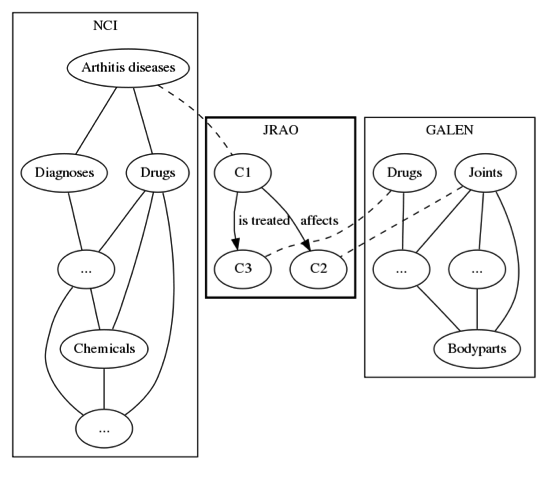
\includegraphics[width=0.6\textwidth]{useCaseOnto3.png}
\caption{JRAO  -- Example for Module Extraction}
\label{JRAO}
\end{center}
\end{figure}


\begin{lstlisting}[basicstyle=\ttfamily,language=dolText,escapechar=@,mathescape]
%prefix( lang:  <http://purl.net/DOL/languages/> )%
library GalenModule
language lang:OWL
ontology myGalen = 
  <http://purl.bioontology.org/ontology/GALEN> extract Drugs, Joints, Bodyparts
end

cons-ext myGalenIsAModule : <http://purl.bioontology.org/ontology/GALEN>
  of  myGalen 
  for Drugs, Joints, Bodyparts
end
\end{lstlisting}
 
%%%%%%%%%%%%%%%%%%%%%%%%%%%%%%%%%%%%%%%%%%%%%%%%%%%%%%%%%%%%%%%%%%%%%%%%%%%%%%%%%%%%%%%%%%%%%%%%%%%%%%%%%%%%%%%%%%%%%%%%%%%%%%%%%%
%%%%%%%%%%%%%%%%%%%%%%%%%%%%%%%%%%%%%%%%%%%%%%%%%%%%%%%%%%%%%%%%%%%%%%%%%%%%%%%%%%%%%%%%%%%%%%%%%%%%%%%%%%%%%%%%%%%%%%%%%%%%%%%%%%

\sclause{Use Case Onto-4: Interoperability Between Closed-World Data and Open-World Metadata}
Data collection has become easier and much more widespread over the years. This data has to be 
assigned a meaning somehow, which occurs traditionally in the  form of metadata annotations. For 
instance, consider geographical datasets derived from satellite data and raw sensor readings. 
Current implementations in, e.g., ecological economics \cite{bagstad_aries_2011} require manual 
annotation of datasets with the information relevant for their processes. While there have been 
attempts to standardize such information \cite{european_comission_inspire_2014}, metadata for 
datasets of simulation results are more difficult to standardize. Moreover, it is 
resource-consuming to link the data to the metadata, to ensure the metadata itself is of good 
quality and consistent, and to actually exploit the metadata when querying the data for data 
analysis. 

The data is usually represented in a database or RDF triple store, which work with a \termref{closed world assumption} on the dataset, and are not expressive enough to 
incorporate the metadata `background knowledge', such as the conditions for validity of the physical laws in the model of the object of observation. These metadata 
require a more expressive language, such as OWL or Common Logic, which operate under an open-world semantics. However, it is unfeasible to translate the 
whole large dataset into OWL or first-order logic. To `meet in the middle', it is possible to declare bridge rules (i.e., a mapping layer) that can link the metadata to 
the data. This approach can be used for intelligent data analysis that combines the data and metadata through querying the system. It enables the analysis of the 
data on the conceptual layer, instead of users having to learn the SQL/SPARQL query languages and how the data is stored. There are various tools and theories 
to realize this, which is collectively called Ontology-Based Data Access/Management, see also \cite{CalvaneseEtAl11}.

The languages for representing the metadata or ontology, for representing the bridge rules or mapping assertions, and for representing the data are different yet 
they need to be orchestrated and handled smoothly in the system, be this for data analytics for large enterprises, for formulating policies, or in silico biology in the 
sciences. 

\DOL  provides the framework for expressing such bridge rules in a systematic way, maintaining these, and building tools for them. 

%%%%%%%%%%%%%%%%%%%%%%%%%%%%%%%%%%%%%%%%%%%%%%%%%%%%%%%%%%%%%%%%%%%%%%%%%%%%%%%%%%%%%%%%%%%%%%%%%%%%%%%%%%%%%%%%%%%%%%%%%%%%%%%%%%
%%%%%%%%%%%%%%%%%%%%%%%%%%%%%%%%%%%%%%%%%%%%%%%%%%%%%%%%%%%%%%%%%%%%%%%%%%%%%%%%%%%%%%%%%%%%%%%%%%%%%%%%%%%%%%%%%%%%%%%%%%%%%%%%%%

\sclause{Use Case Onto-5: Verification of Rules Translating Dublin Core Into PROV}
The Dublin Core Metadata terms, which have been formalized as an RDF Schema vocabulary, developed initially by the digital library community, are less 
comprehensive but more widely used than PROV (cf.\ subclause~\ref{onto-1}). The rules for translating Dublin Core to the OWL subset of PROV (and, with restrictions, 
vice versa) are not known to yield valid instances of the PROV data model, i.e.\ they are not known to yield OWL ontologies consistent with respect to the OWL axioms that 
capture part of the PROV data model. This may disrupt systems that would like to reason about the provenance of an entity, and thus the assessment of the 
entity's quality, reliability or trustworthiness.
The Dublin Core to PROV ontology translation%
\footnote{\url{http://www.w3.org/TR/2013/NOTE-prov-dc-20130430/}}
  is expressed partly by a symbol mapping and partly by FOL rules. These FOL rules are implemented by CONSTRUCT patterns in the SPARQL RDF query language.%
\footnote{E.g., \url{http://www.w3.org/TR/2013/NOTE-prov-dc-20130430/\#dct-creator}} 
SPARQL has a formal specification of the evaluation semantics of its algebraic expressions, which 
 is different from the model-theoretic semantics of the OWL and RDF Schema languages; nevertheless 
SPARQL CONSTRUCT is a popular and immediately executable syntax for expressing translation rules 
 between ontologies in RDF-based languages in a subset of FOL.
\DOL  not only supports the reuse of the existing Dublin Core RDF Schema and PROV OWL ontologies as 
 modules of a distributed ontology (= OMS network), but it is also able to support the description 
of the FOL translation rules in a sufficiently expressive ontology language, e.g. Common Logic, 
and thus enable formal verification of the translation from Dublin Core to PROV.


%%%%%%%%%%%%%%%%%%%%%%%%%%%%%%%%%%%%%%%%%%%%%%%%%%%%%%%%%%%%%%%%%%%%%%%%%%%%%%%%%%%%%%%%%%%%%%%%%%%%%%%%%%%%%%%%%%%%%%%%%%%%%%%%%%
%%%%%%%%%%%%%%%%%%%%%%%%%%%%%%%%%%%%%%%%%%%%%%%%%%%%%%%%%%%%%%%%%%%%%%%%%%%%%%%%%%%%%%%%%%%%%%%%%%%%%%%%%%%%%%%%%%%%%%%%%%%%%%%%%%

\sclause{Use Case Onto-6: Maintaining Different Versions of an Ontology 
in Languages with Different Expressivity}
Often it is useful to maintain different versions of an ontology within languages, which differ in 
 their expressivity. 
 
 
For example,  DOLCE is a foundational ontology that has primarily been formalized in
 the first-order logic 
ontology language KIF (a predecessor of Common Logic), but also in OWL (``DOLCE Lite'') 
\cite{dolce}. This ``OWLized'' version was targeting use in semantic web services and domain 
ontology interoperability, and to provide the generic categories and relationships to aid 
 domain ontology development. DOLCE has been used also for semantic middleware, and in 
OWL-formalized ontologies of different domains, including neuroimaging, computing, and ecology.
  Given the differences in expressivity between KIF and OWL, DOLCE Lite 
   had to simplify certain notions.  For example, 
 the DOLCE Lite formalization of ``temporary parthood'' (something is part of something else at a 
certain point or interval in time) omits any information about the time, as OWL only supports 
binary predicates (a.k.a.\ ``properties'').  That leaves ambiguities for modeling a view from
DOLCE Lite to the first-order DOLCE, as such a view would have to reintroduce the third (temporal) 
component of such predicates:
  \begin{itemize}
  \item Should a relation asserted in terms of DOLCE Lite be assumed to hold for \emph{all} possible points/intervals in time, \ie should it be universally quantified?
  \item Or should such a relation be assumed to hold for \emph{some} points/intervals in time, \ie should it be existentially quantified?
  \item Or should a concrete value for the temporal component be assumed, \eg ``0'' or ``now''?
  \end{itemize}
%  
\DOL supports the formalization of  all of these views. Given suitable consistency 
checking tools, DOL enables the analysis of  whether any such view satisfies all further
 axioms that the  first-order DOLCE states about temporal parthood.

%%%%%%%%%%%%%%%%%%%%%%%%%%%%%%%%%%%%%%%%%%%%%%%%%%%%%%%%%%%%%%%%%%%%%%%%%%%%%%%%%%%%%%%%%%%%%%%%%%%%%%%%%%%%%%%%%%%%%%%%%%%%%%%%%%
%%%%%%%%%%%%%%%%%%%%%%%%%%%%%%%%%%%%%%%%%%%%%%%%%%%%%%%%%%%%%%%%%%%%%%%%%%%%%%%%%%%%%%%%%%%%%%%%%%%%%%%%%%%%%%%%%%%%%%%%%%%%%%%%%%

\sclause{Use Case Onto-7: Metadata within OMS Repositories}
DOL provides a language for the metadata within OMS Repositories. 
For example, the Common Logic Repository (COLORE) \footnote{\url{http://stl.mie.utoronto.ca/colore/}} is an open 
repository of more than 150 ontologies as of December 2011, all formalized in Common Logic. 
COLORE  stores metadata about its ontologies, which are represented using a custom XML schema that 
covers the following aspects\footnote{\url{http://stl.mie.utoronto.ca/colore/metadata.html}}, 
without specifying a formal semantics for them:
  \begin{description}
  \item[module provenance] author, date, version, description, keyword, parent 
ontology\footnote{Note that this use of the term ``module'' in COLORE corresponds
to the term \termref{structured OMS} in this \IS{}.}
  \item[axiom source provenance] name, author, year\footnote{Note that this may cover any 
   sentences\index{sentence} in the sense of this \IS{}.}
  \item[direct relations] maps (signature morphisms), definitional extension, conservative 
   extension, inconsistency between ontologies, imports, relative interpretation, faithful 
interpretation, definable equivalence
  \end{description}

  \DOL provides built-in support for a subset of the ``direct relations'' and specifies a formal 
semantics for them.  In addition, it supports the implementation of  the remainder of the COLORE 
metadata vocabulary as an ontology, reusing suitable existing metadata vocabularies such as OMV, 
and it supports the implementation of one or multiple Common Logic ontologies plus their 
annotations as one coherent \DOL library.

%%%%%%%%%%%%%%%%%%%%%%%%%%%%%%%%%%%%%%%%%%%%%%%%%%%%%%%%%%%%%%%%%%%%%%%%%%%%%%%%%%%%%%%%%%%%%%%%%%%%%%%%%%%%%%%%%%%%%%%%%%%%%%%%%%
%%%%%%%%%%%%%%%%%%%%%%%%%%%%%%%%%%%%%%%%%%%%%%%%%%%%%%%%%%%%%%%%%%%%%%%%%%%%%%%%%%%%%%%%%%%%%%%%%%%%%%%%%%%%%%%%%%%%%%%%%%%%%%%%%%

\sclause{Use Case Spec-1: Modularity of Specifications}\label{spec-1}
Often specifications become so large that it is necessary to structure
them in a modular way, for human readability and maintainability, and for more efficient tool support. The lack of a standard for such
modular structuring hinders interoperability among different
development efforts and the reuse of specifications.  \DOL provides a
notion of structured modular specification that is equally applicable
to all \DOL-conforming logical languages.

Structuring pays off even for small specifications. For example, it makes
structuring a simple specification of sorting lists in the 
following way enhances both readability and potential for re-use
of specifications:

\begin{lstlisting}[basicstyle=\ttfamily\footnotesize,language=dolText,alsolanguage=CASL,escapechar=@,mathescape]	
%prefix( lang:  <http://purl.net/DOL/languages/> )%

library Sorting

language lang:CASL
%right_assoc __::__
spec TotalOrder =
  sort Elem
  pred __<=__ : Elem * Elem
  forall x,y,z : Elem
  . x <= x                         %(reflexive)%
  . x <= z if x <= y /\ y <= z     %(transitive)%
  . x = y if x <= y /\ y <= x      %(antisymmetric)%
  . x <= y \/ y <= x               %(dichotomous)%
end

spec Nat =
  free type Nat ::= 0 | suc(Nat)
end

spec List =
  Nat
then
  sort Elem
  free type List ::= [] | __::__(Elem; List)
  op count : Elem * List -> Nat
  forall x,y : Elem; L : List
  . count(x,[]) = 0
  . count(x,x :: L) = suc(count(x,L))
  . count(x,y :: L) = count(x,L) if not x=y
end

spec Sorting =
  TotalOrder and List
then
  preds is_ordered : List;
        permutation : List * List
  vars x,y:Elem; L,L1,L2:List
  . is_ordered([])
  . is_ordered(x::[])
  . is_ordered(x::y::L) <=> x<=y /\ is_ordered(y::L)
  . permutation(L1,L2) <=> (forall x:Elem . count(x,L1) = count(x,L2))
then
  op sorter : List->List
  var L:List
  . is_ordered(sorter(L))
  . permutation(L,sorter(L))
hide is_ordered, permutation
end
\end{lstlisting}

In the last step, the structuring operation of hiding is used to
restrict the specification to an export interface: 
 predicates \texttt{is\_ordered} and \texttt{permutation} are hidden, because they
are only auxiliary and need not be implemented.


%%%%%%%%%%%%%%%%%%%%%%%%%%%%%%%%%%%%%%%%%%%%%%%%%%%%%%%%%%%%%%%%%%%%%%%%%%%%%%%%%%%%%%%%%%%%%%%%%%%%%%%%%%%%%%%%%%%%%%%%%%%%%%%%%%
%%%%%%%%%%%%%%%%%%%%%%%%%%%%%%%%%%%%%%%%%%%%%%%%%%%%%%%%%%%%%%%%%%%%%%%%%%%%%%%%%%%%%%%%%%%%%%%%%%%%%%%%%%%%%%%%%%%%%%%%%%%%%%%%%%

\sclause{Use Case Spec-2: Specification Refinements}\label{spec-2}
Formal software and hardware development methods are often used to
ensure the correct function of systems which have safety-critical
requirements or which may not be easily accessible for repair or
replacement.  Examples of such requirements can be found in
safety-critical areas such as medical systems, or in the automotive,
avionics and aerospace industries, as well as in components used by
those industries such as in microprocessor design.

Typically, a requirement specification is refined into a
design specification and then an implementation, often involving
several intermediate steps (see, e.g. the V-model~\cite{V-model}, although
this does not require formal specification).  There are numerous
specification formalisms in use, including the OMG's SysML language;
moreover, often during development, the formalism needs to be changed
(e.g. from a specification to a programming language, or from a
temporal logic to a state machine). For each of these formalisms,
notions of refinement have been defined and implemented. However, the
lack of a standardized, logically sound language and methodology for
such refinement hinders interoperability among different development
efforts and the reuse of refinements.  \DOL provides the capability to
represent refinement that is equally applicable to all \DOL-conforming
logical languages, and that covers at least the most relevant of the
industrial use cases of specification refinement.

A simple example is the refinement of the (purely declarative) sorting
specification from use case in section \ref{spec-1} into a specification of a particular sorting
algorithm (for simplicity, insert sort is used for demonstration):

\begin{lstlisting}[basicstyle=\ttfamily\footnotesize,language=dolText,alsolanguage=CASL,escapechar=@,mathescape]	
spec InsertSort = 
  TotalOrder and List
then
  ops insert : Elem*List -> List;
      insert_sort : List->List
  vars x,y:Elem; L:List
  . insert(x,[]) = x::[]
  . insert(x,y::L) = x::insert(y,L) when x<=y else y::insert(x,L)
  . insert_sort([]) = []
  . insert_sort(x::L) = insert(x,insert_sort(L))
 hide insert
end

%% refinement from abstract sorting to insert sort
refinement InsertSortCorrectness =
   Sorting refined via sorter |-> insert_sort to InsertSort
end
\end{lstlisting}
Note that hiding is essential here to make the signatures of
both specifications compatible. If  the
predicates \texttt{is\_ordered} and \texttt{permutation}
had not been hidden in the \texttt{Sorting} specification, a refinement would
not have been possible, since \texttt{InsertSort} does not
implement these predicates (and it would be rather artificial
to add an implementation for them).

\medskip

Refinements can be composed. A simple example below illustrates this
by expressing that natural numbers with addition form a monoid, and
that natural numbers can be efficiently represented for implementation
as lists of binary digits, together with several equivalent ways of
composing these refinements.

\begin{lstlisting}[basicstyle=\ttfamily\footnotesize,language=dolText,alsolanguage=CASL,escapechar=@,mathescape]	
spec Monoid =
 sort Elem
 ops 0 : Elem;
         __+__ : Elem * Elem -> Elem, assoc, unit 0
end

spec NatWithSuc = %mono
 free type Nat ::= 0 | suc(Nat)
 op __+__ : Nat * Nat -> Nat, unit 0 
 forall x , y : Nat . x + suc(y) = suc(x + y)
 op 1:Nat = suc(0)
end

spec Nat =
  NatWithSuc hide suc
end

spec NatBin =
generated type Bin ::= 0 | 1 | __0(Bin) | __1(Bin)

ops __+__ , __++__ : Bin * Bin -> Bin 
forall x, y : Bin 
 .  0 0 = 0  .  0 1 = 1
 .  not  (0 = 1)  .  x 0 = y 0 => x = y .  not  (x 0 = y 1)  .  x 1 = y 1 => x = y
 .  0 + 0 = 0  .  0 ++ 0 = 1 
 .  x 0 + y 0 = (x + y) 0  .  x 0 ++ y 0 = (x + y) 1
 .  x 0 + y 1 = (x + y) 1  .  x 0 ++ y 1 = (x ++ y) 0 
 .  x 1 + y 0 = (x + y) 1  .  x 1 ++ y 0 = (x ++ y) 0
 .  x 1 + y 1 = (x ++ y) 0  .  x 1 ++ y 1 = (x ++ y) 1 
end

refinement R1 =
 Monoid refined via Elem |-> Nat to Nat
end

refinement R2 =
 Nat refined via Nat |-> Bin to NatBin
end

refinement R3 =
 Monoid refined via Elem |-> Nat to
 Nat refined via Nat |-> Bin to NatBin
end

refinement R3' =
 Monoid refined via Elem |-> Nat to R2
end

refinement R3'' = 
 Monoid refined via Elem |-> Nat to Nat refined to R2
end

refinement R3''' = R1 refined to R2

\end{lstlisting}

It can be useful to also consider refinement of networks of OMS.
Suppose that the specification \syntax{Nat} is extended in different
ways: by a specification \syntax{Int} of integers, as well
as by a specification \syntax{List} of lists.
These three specifications form a network, see Fig.~\ref{fig:simple-network}.
The network expresses the distributed character of the development:
some people might use only \syntax{Int}, others only \syntax{List},
so there is no necessity to unite all specifications into one
large specification. 
\begin{lstlisting}[basicstyle=\ttfamily\footnotesize,language=dolText,alsolanguage=CASL,escapechar=@,mathescape]
spec Int = %mono
  Nat
then %mono
     generated type Int ::= __ - __(Nat;Nat)
     forall a,b,c,d: Nat
     .  a - b = c - d <=> a + d = c + b    %(equality_Int)%
     sort  Nat < Int
     forall a: Nat . a = a - 0             %(Nat2Int_embedding)%
end

spec List = 
  Nat 
then 
  sort Elem
  free type List ::=  [] |  __ :: __ (Elem; List)
     op   #__: List -> Nat;
     forall x,: Elem; L: List
     . # [] = 0                              %(numberOf_nil_List)%
     . # (x :: L) = suc( # L )               %(numberOf_NeList_List)%
end

network NatIntList = Nat, Int, List
end
\end{lstlisting}

\begin{figure}
$$\xymatrix{
\Text{Int} && \Text{List}\\
& \Text{Nat} \ar[ru] \ar[lu]
}$$
\caption{An OMS network consisting of three specifications
\label{fig:simple-network}}
\end{figure}

The network in Fig.~\ref{fig:simple-network} can be refined
to a network that is closer to implementation.
This amounts to refining the specifications of the network
individually, see Fig.~\ref{fig:simple-network-refinement}.
This needs to be done in such a way that both the refinement of \syntax{Int} 
and that of \syntax{List} are to built over the refinement of \syntax{Nat}.
\begin{lstlisting}[basicstyle=\ttfamily\footnotesize,language=dolText,alsolanguage=CASL,escapechar=@,mathescape]
spec IntBin = NatBin then ...
end
spec ArrayWithPointer = NatBin then ...
end
network NatIntListImpl = NatBin, IntBin, ArrayWithPointer
end
refinement NetworkRefinement = 
  NatIntList refined via 
      R2, %% Nat is refined to NatBin, see above
      Int refined via sort Int |-> BinInt to IntBin,
      List via sort List |-> Array to ArrayWithPointer
    to NatIntListImpl
end
\end{lstlisting}

\begin{figure}
$$\xymatrix{
\Text{Int}\ar@/^2.0pc/@[red][rrrrr] && \Text{List}\ar@/^2.0pc/@[red][rrrrr] &&& \Text{BinInt} && \Text{ArrayWithPointer}\\
& \Text{Nat}\ar@/_2.0pc/@[red][rrrrr] \ar[ru] \ar[lu] &&&&& \text{Bin}\ar[ru] \ar[lu] & \\
&&\\
&\Text{NatIntList}\ar@[red][rrrrr] &&&&& \Text{NatIntListImpl}
}$$
\caption{A refinement between OMS networks
\label{fig:simple-network-refinement}}
\end{figure}

%%%%%%%%%%%%%%%%%%%%%%%%%%%%%%%%%%%%%%%%%%%%%%%%%%%%%%%%%%%%%%%%%%%%%%%%%%%%%%%%%%%%%%%%%%%%%%%%%%%%%%%%%%%%%%%%%%%%%%%%%%%%%%%%%%
%%%%%%%%%%%%%%%%%%%%%%%%%%%%%%%%%%%%%%%%%%%%%%%%%%%%%%%%%%%%%%%%%%%%%%%%%%%%%%%%%%%%%%%%%%%%%%%%%%%%%%%%%%%%%%%%%%%%%%%%%%%%%%%%%%


\sclause{Use Case Model-1: Consistency Among UML Models of Different Types}
\label{model-1}

A typical UML model involves models of different types. Such UML models may have intrinsic errors because models of different types may specify conflicting 
requirements. Typical questions that arise in this context ask for
semantic consistency, e.g.,

\begin{itemize}
\item whether the multiplicities in a class model are semantically consistent with each other;
%\item whether the attributes and operations in a state machine are
%available in a class diagram;
\item	  whether the sequential composition of actions in an interaction diagram is justified by an accompanying OCL specification;
\item 	whether cooperating state machines comply with pre-/post-conditions and invariants;
\item 	whether the behavior prescribed in an interaction model is realizable by several state machines cooperating according to a composite structure model.
\end{itemize}
Such questions are currently hard to answer in a systematic manner. One method to answer these questions and find such errors is a check for semantic 
consistency. Under some restrictions, the proof of semantic consistency can be (at least partially) performed using model-checking tools like Hugo/RT \cite{knapp-wuttke:models06wsh:2007}. 
Once a formal semantics for the different model types has been chosen (see, e.g. \cite{knapp-mossakowski-roggenbach:corr:2014}), it is possible to use \DOL to specify in which 
sense the models need to be consistent, and check this by suitable tools.

%%%%%%%%%%%%%%%%%%%%%%%%%%%%%%%%%%%%%%%%%%%%%%%%%%%%%%%%%%%%%%%%%%%%%%%%%%%%%%%%%%%%%%%%%%%%%%%%%%%%%%%%%%%%%%%%%%%%%%%%%%%%%%%%%%

\ssclause{The ATM Example}
\label{sec:atm-example}

 The ATM example, which illustrates model-driven development using UML,
is taken from \cite{knapp-mossakowski-roggenbach:corr:2014}.  The example involves
the design of a traditional automatic teller machine (ATM) connected
to a bank. For simplicity,  the example focuses
 on the ATM's processing of card and PIN entry actions.  
After entering the card, one has three
trials for entering the correct PIN (which is checked by the
bank). After three unsuccessful trials the card is kept.

\begin{figure}[!ht]
\centering
\subfigure[Interaction\label{fig:interaction}]{%
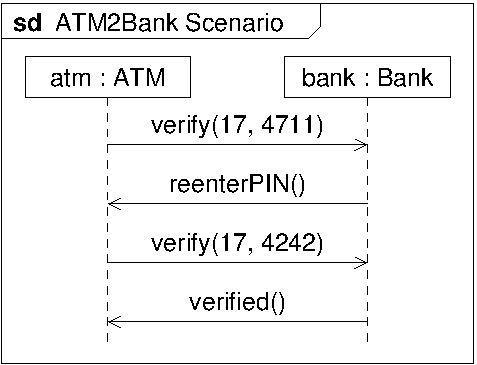
\includegraphics[scale=.5]{illustrations/uml/sd-atm2bank.pdf}
%  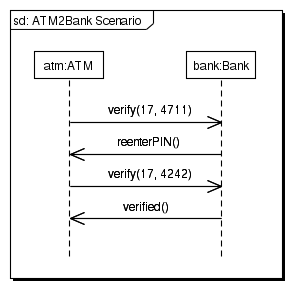
\includegraphics[trim=6 6 6 6,clip,scale=0.65]{illustrations/uml/scenario.png}%\\[-1.5ex]
}
\hspace*{0.5cm}
\subfigure[Composite structure\label{fig:system}]{%
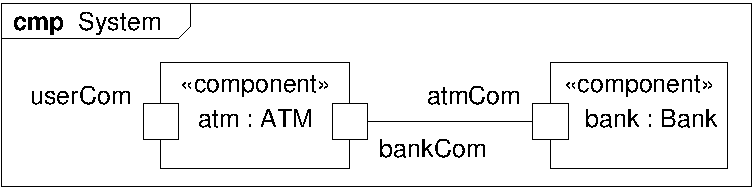
\includegraphics[scale=.5]{illustrations/uml/cmp-system.pdf}
%  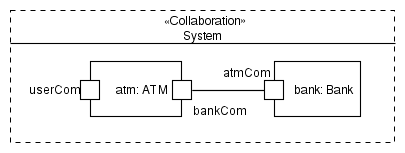
\includegraphics[trim=6 6 6 6,clip,scale=0.65]{illustrations/uml/system.png}%\\[-1.5ex]
}
\\
\subfigure[Protocol state machine\label{fig:psm}]{%
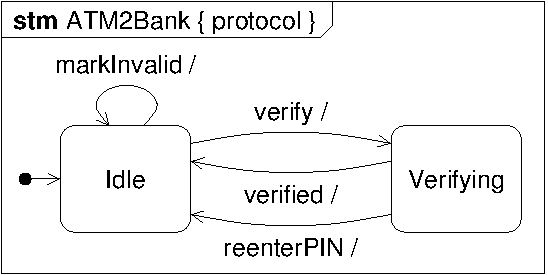
\includegraphics[scale=.5]{illustrations/uml/stm-atm2bank-protocol.pdf}
%  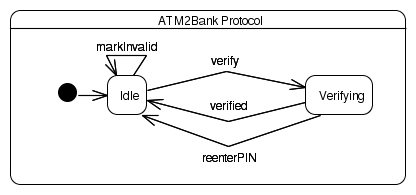
\includegraphics[trim=6 6 6 6,clip,scale=.65]{illustrations/uml/protocol.png}%\\[-1.5ex]
}
\hspace*{0.4cm}
\subfigure[Interfaces and components\label{fig:class}]{%
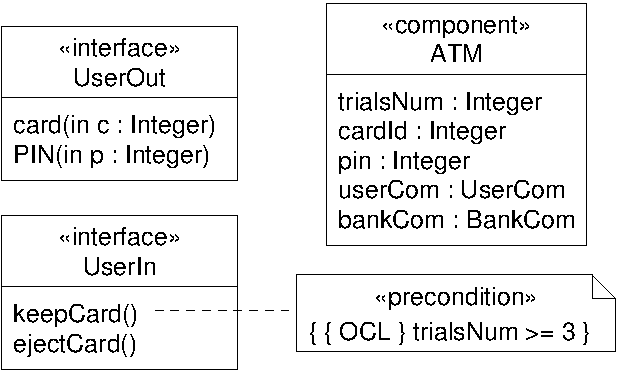
\includegraphics[scale=.5]{illustrations/uml/pkg-components.pdf}
%  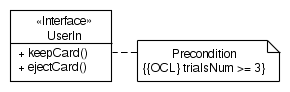
\includegraphics[trim=6 6 6 6,clip,scale=0.65]{illustrations/uml/interfaceWithOCL.png}%\\[-1.5ex]
}
\\
\subfigure[State machine\label{fig:state-machine}]{%
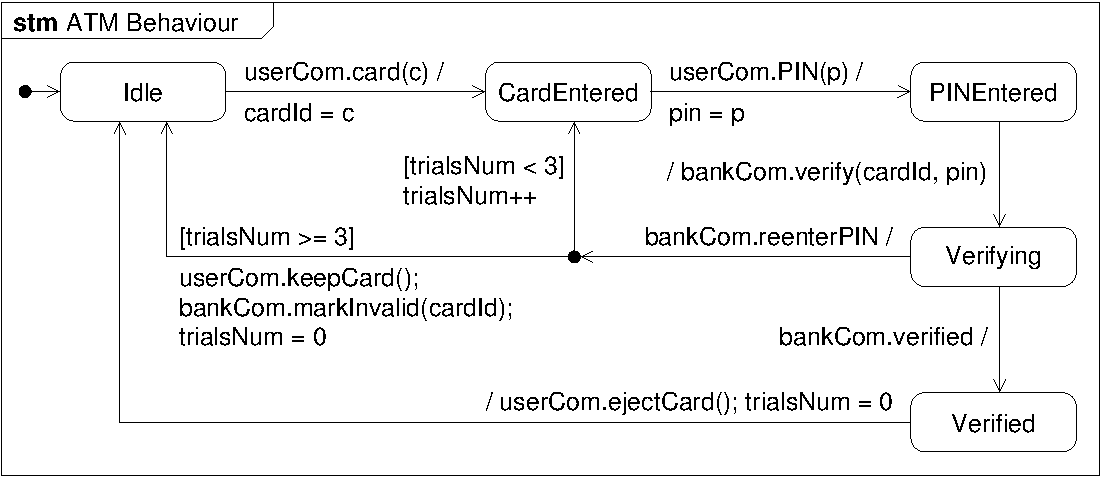
\includegraphics[scale=.5]{illustrations/uml/stm-atm-behaviour.pdf}
%  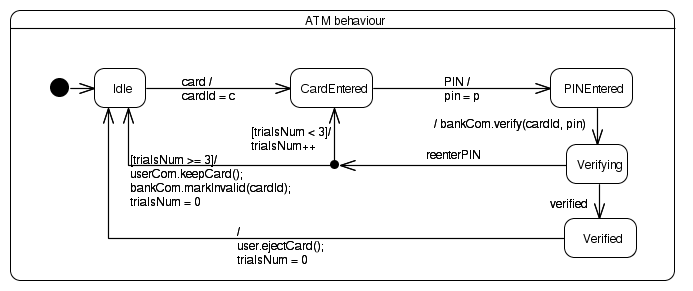
\includegraphics[trim=6 6 6 6,clip,scale=0.65]{illustrations/uml/atm-behaviour.png}%\\[-1.5ex]
}
\vspace*{-1.5ex}
\caption{ATM example}\label{fig:atm-example}
\end{figure}

\fref{fig:interaction} shows a possible \emph{interaction} between
an \uml{atm} and a \uml{bank} object, which consists of four messages:
the \uml{atm} requests the \uml{bank} to \uml{verify} if a card and PIN
number combination is valid, in the first case the \uml{bank} requests
to reenter the PIN, in the second case the verification is successful.
This interaction presumes that the system has an \uml{atm} and a
\uml{bank} as objects. This can, e.g., be ensured by a \emph{composite
  structure model}, see Fig.~\ref{fig:system}, which -- among other
things -- specifies the objects in the initial system state.
Furthermore, it specifies that the communication between \uml{atm} and
\uml{bank} goes through the two ports \uml{bankCom} and \uml{atmCom}
linked by a connector.  The communication protocol on this connector is
captured with a \emph{protocol state machine}, see Fig.~\ref{fig:psm}.
The protocol state machine fixes in which order the messages
\uml{verify}, \uml{verified}, \uml{reenterPIN}, and \uml{markInvalid}
between \uml{atm} and \uml{bank} may occur.  Figure~\ref{fig:class}
provides structural information in form of interfaces specifying what is
provided and required at the \uml{userCom} port and the \uml{bankCom}
port of the \uml{atm} instance.  An interface is a set of operations
that other model elements have to implement. In our case, the
interfaces are described in a \emph{class model}. Its component type 
\uml{ATM} is further enriched with the OCL
constraint \uml{trialsNum <= 3}, which refines its semantics requiring
that \uml{trialsNum} must not exceed three.

Finally, the dynamic behavior of the \uml{atm} object is specified by
the \emph{behavioral state machine} shown in
Fig.~\ref{fig:state-machine}. The machine consists of five states
including \uml{Idle}, \uml{CardEntered}, etc.  Beginning in the
initial \uml{Idle} state, the user can \emph{trigger} a state change
by entering the \uml{card}. This has the \emph{effect} that the
parameter \uml{c} from the \uml{card} event is assigned to the
\uml{cardId} in the \uml{atm} object (parameter names are not shown on
triggers). Entering a \uml{PIN} triggers another transition to
\uml{PINEntered}.  Then the ATM requests verification from the bank
using its \uml{bankCom} port.  The transition to \uml{Verifying} uses
a \emph{completion event}: No explicit trigger is declared and the
machine autonomously creates such an event whenever a state is
completed, i.e., all internal activities of the state are finished (in
our example there are no such activities).  If the interaction with
the bank results in \uml{reenterPIN}, and the \emph{guard}
\uml{trialsNum < 3} is true, the user can again enter a \uml{PIN}.


The ATM example in Fig.~\ref{fig:atm-example} consists of five different
UML models, which naturally form a network. Coherence of this network is
expressed as its consistency.  It is assumed that XMI \nref{XMI} representations of
the relevant UML models have been stored at
\url{http://www.example.org/uml/} in a single xmi-file \url{http://www.example.org/uml/atm.xmi} that contains a
\texttt{uml:Model} element for each UML model whose \texttt{xmi:id} has
a prefix \texttt{xxx} followed by an underscore. \texttt{xxx} is determined 
as follows:\medskip

\begin{tabular}{|l|l|l|}\hline
\textbf{Figure} & \textbf{\texttt{xxx}} & \textbf{diagram type}\\\hline
Fig.~\ref{fig:interaction} & sd & sequence diagram\\\hline
Fig.~\ref{fig:system} & cmp & composite structure diagram\\\hline
Fig.~\ref{fig:psm} & psm & protocol state machine\\\hline
Fig.~\ref{fig:class} & cd & class diagram\\\hline
Fig.~\ref{fig:state-machine} & stm & state machine\\\hline
\end{tabular}

\begin{lstlisting}[basicstyle=\ttfamily,language=dolText,escapechar=@,mathescape]
%prefix( :      <http://www.example.org/uml/>
         uml:   @<http://www.uml.org/spec/UML/>@
         log:   <http://purl.net/DOL/logics/> )%
                %% descriptions of logics ...
library ATM

refinement cd2stm = cd refined to { atm hide along stm2cd} end
refinement cd2psm = cd refined to { psm hide along psm2cd} end
network ATM_network = %consistent
                      cd, stm, psm, cmp,
                      cd2stm, cd2psm, abstract_to_concrete_atm
end
entailment atm = ATM_network entails sd
network Some_refined_ATM_network = ... end
refinement r = ATM_network refined to Some_refined_ATM_network
entailment e = Some_refined_ATM_network entails ATM_network
\end{lstlisting}
Here, \texttt{abstract\_to\_concrete\_atm} is defined in the next
section, and \texttt{stm2cd} and \texttt{psm2cd} are suitable logic
projections extracting the classes, attributes and operations from a
(protocol) state machine, delivering a class model.


%%%%%%%%%%%%%%%%%%%%%%%%%%%%%%%%%%%%%%%%%%%%%%%%%%%%%%%%%%%%%%%%%%%%%%%%%%%%%%%%%%%%%%%%%%%%%%%%%%%%%%%%%%%%%%%%%%%%%%%%%%%%%%%%%%
%%%%%%%%%%%%%%%%%%%%%%%%%%%%%%%%%%%%%%%%%%%%%%%%%%%%%%%%%%%%%%%%%%%%%%%%%%%%%%%%%%%%%%%%%%%%%%%%%%%%%%%%%%%%%%%%%%%%%%%%%%%%%%%%%%

\sclause{Use Case Model-2: Refinements Between UML Models of Different Types, and Their Reuse}
\label{model-2}

A problem is a lack of reusability of refinements: Consider a controller for an elevator, which is specified with a UML protocol state machine, enriched with UML 
sequence models and OCL constraints. Assume further that this UML model is not directly implemented, but first refined to a UML behavior state machine (which then 
can be automatically or semi-automatically transformed into some implementation using standard UML tools). However, there is no standardized language to 
express, document and maintain the refinement relation itself (UML only allows very simple refinements, namely between state machines). This hinders both the 
reuse of such refinements in different contexts, as well as the interoperability of tools proving such refinements to be correct. \DOL  
addresses these problems by providing a standardized notation with formal semantics for such refinements. Refinements expressed in this language could, e.g., be 
parameterized and reused in different contexts.

 This can be illustrated based on the state
machine of the \uml{atm}, shown in Fig.~\ref{fig:state-machine}, which is a  
refinement of the protocol state machine in Fig.~\ref{fig:psm}. This can be stated as follows in \DOL. 
\footnote{  It is assumed that XMI representations of the relevant UML models have been 
stored at \url{http://www.example.org/uml/},
e.g.\ \url{http://www.example.org/uml/atm.xmi} } 


\begin{lstlisting}[basicstyle=\ttfamily,language=dolText,escapechar=@,mathescape]
refinement abstract_to_concrete_atm =
  psm refined via translation psm2sm to { atm and bank }
end
\end{lstlisting}

The refinement uses an abstraction of the \uml{atm}, expressed by the
translation via symbol map \texttt{Idle |-> Idle, CardEntered |-> Idle, PINEntered |-> Idle, Verified |-> Idle, Verifying |-> Verifying}, resulting in a two-state machine. Moreover, some detail of the \uml{atm} is hidden using
\syntax{hide}. Then, the protocol state machine can be refined to
the thus abstracted \uml{atm}.

%%%%%%%%%%%%%%%%%%%%%%%%%%%%%%%%%%%%%%%%%%%%%%%%%%%%%%%%%%%%%%%%%%%%%%%%%%%%%%%%%%%%%%%%%%%%%%%%%%%%%%%%%%%%%%%%%%%%%%%%%%%%%%%%%%
%%%%%%%%%%%%%%%%%%%%%%%%%%%%%%%%%%%%%%%%%%%%%%%%%%%%%%%%%%%%%%%%%%%%%%%%%%%%%%%%%%%%%%%%%%%%%%%%%%%%%%%%%%%%%%%%%%%%%%%%%%%%%%%%%%

\sclause{Use Case Model-3: Coherent Semantics for Multi-Language Models}
\label{model-3}
	
Often a single problem area within a given domain must be represented using several formalisms, e.g., because of user community requirements, expressiveness or tool support 
and usage. 
Typically the different representations are written by different people using formalisms that are based on different logics. Thus, it is a challenge to maintain 
consistency across the different representations. 
The need for the use of multiple OMS languages, even within the OMG community, is also reflected by the OMG Ontology Definition Metamodel (ODM, \nref{ODM}), which 
provides a number of syntactic transformations between such languages.
One example is the OMG Date-Time Vocabulary (DTV, \nref{DTV}). DTV has been formulated in different languages, each of which addresses different audiences:
\begin{itemize}
\item	 SBVR \nref{SBVR}: business users
\item 	UML \nref{UML} (class models and OCL): software implementors
\item 	OWL \nref{OWL2}: ontology developers and users
\item 	Common Logic \nref{CL}: (foundational) ontology developers and users
\end{itemize}
With \DOL, one can, e.g.,
\begin{itemize}
\item 	formally relate the different formalizations used for DTV, relate the different formalizations using translations,
\item 	check consistency across the different formalizations (using suitable tools),
\item 	extract sub-modules covering specific aspects, and
\item 	specify the OWL version to be an approximation of the Common Logic version (using a heterogeneous interpretation of OMS).
\end{itemize}
Note that the last point does not specify what information is lost in the approximation. Indeed, \DOL provides the means to specify requirements on the approximation, e.g., that it maximally preserves the information. 

Coming to a \DOL example,
a UML model like the ATM model developed in section \ref{sec:atm-example} typically is part of an
application context that also contains some common terminology.
This terminology often is specified by an ontology, and then
it is desirable to relate the model to the ontology. Consider
the following financial ontology fragment:

\begin{lstlisting}[basicstyle=\ttfamily,language=dolText,alsolanguage=owl2Manchester,escapechar=@,mathescape]
ontology myTaxonomy =
  ObjectProperty: owns
    Characteristics: Irreflexive, Asymmetric

  Class: FinancialIntermediary
    SubClassOf: CorporatePerson
  Class: CorporatePerson
    SubClassOf: ImmaterialEntity
  Class: ImmaterialEntity
    DisjointWith: MaterialEntity
    SubClassOf: has_part only ImmaterialEntity
  Class: Livestock
    SubClassOf: MaterialEntity
  %% ...
end
\end{lstlisting}

 To relate this ontology with the ATM model, 
various aspects need to be taken care of:
\begin{itemize}
  \item Translating into shared language  (in this case, Common Logic)
  \item Unifying terminology (Bank vs. FinancialIntermediary)
  \item Connecting related concepts (bank.owns.ATM vs. owns)
  \item Removing irrelevant parts (livestock) 
\end{itemize}

\begin{lstlisting}[basicstyle=\ttfamily\small,language=dolText,alsolanguage=owl2Manchester,escapechar=@,mathescape]
model xmiStateModel = <https://ontohub.org/ATM/state.xmi> end

model clStateModel = xmiStateModel with
                     translation UMLState2CL
end

model xmiClassModel = <https://ontohub.org/ATM/class.xmi> end

model clClassModel = xmiClassModel with
            translation UMLClass2CL
            Bank |-> FinancialIntermediary
end

ontology BigTaxonomy = <https://ontohub.org/ATM/mytaxonmy.owl> end

ontology NoLivestockTaxonomy = BigTaxonomy reject
                               { Class: Livestock }
end

ontology ExtendedTaxonomy = NoLivestockTaxonomy then
         ObjectProperty: FinancialIntermediary.owns.ATM
           SubPropertyOf: owns
           Domain: FinancialIntermediary
           Range: ATM
end

ontology clTaxonomy = ExtendedTaxonomy with
                      translation OWL22CommonLogic

oms JointModel = clStateModel and
                 clClassModel and
                 clTaxonomy
end
\end{lstlisting}

%%%%%%%%%%%%%%%%%%%%%%%%%%%%%%%%%%%%%%%%%%%%%%%%%%%%%%%%%%%%%%%%%%%%%%%%%%%%%%%%%%%%%%%%%%%%%%%%%%%%%%%%%%%%%%%%%%%%%%%%%%%%%%%%%%
%%%%%%%%%%%%%%%%%%%%%%%%%%%%%%%%%%%%%%%%%%%%%%%%%%%%%%%%%%%%%%%%%%%%%%%%%%%%%%%%%%%%%%%%%%%%%%%%%%%%%%%%%%%%%%%%%%%%%%%%%%%%%%%%%%

\sclause{Conclusion}

In this section, several use cases have been introduced. They illustrate many aspects of DOL and its usefulness in many situations in which different OMS artifacts might be leveraged and augmented to produce broader or more tractable models, ontologies, and specifications.

 \DOL has been designed to support of a wide range of formalisms and
provides the ability to specify the basis for formal interoperability even among heterogeneous OMS and OMS networks. \DOL enables the solutions of the problems described in the use cases above. It also enables the development of DOL documents, tools and workflows that 
allow  a better exchange and reuse of OMS. Eventually, this will also lead to better, easier developed and maintained systems based on these OMS.

The next sections present the metalanguage \DOL{}; in particular, the syntax and the model-theoretic semantics. Further, various features of \DOL will be discussed, which  are based on  best practices of modularity  across
 the three areas of ontology design, formal 
specification, and model-driven development.


%%%%%%%%%%%%%%%%%%%%%%%%%%%%%%%%%%%%%%%%%%%%%%%%%%%%%%%%%%%%%%%%%%%%%%%%%%%%%%%%%%%%%%%%%%%%%%%%%%%%%%%%%%%%%%%%%%%%%%%%%%%%%%%%%%
%%%%%%%%%%%%%%%%%%%%%%%%%%%%%%%%%%%%%%%%%%%%%%%%%%%%%%%%%%%%%%%%%%%%%%%%%%%%%%%%%%%%%%%%%%%%%%%%%%%%%%%%%%%%%%%%%%%%%%%%%%%%%%%%%%
%%%%%%%%%%%%%%%%%%%%%%%%%%%%%%%%%%%%%%%%%%%%%%%%%%%%%%%%%%%%%%%%%%%%%%%%%%%%%%%%%%%%%%%%%%%%%%%%%%%%%%%%%%%%%%%%%%%%%%%%%%%%%%%%%%

\cleardoublepage
\clauseI{Design Overview} \label{c:design}
\sclause{General}
%\ednote{replace this section by saying how we respond to the RFP}
%
%\CLnote[type=todo]{Get rid of formal \should/\shall language (e.g.\ in clause headers: \should/\shall applies to conforming implementations anyway, rather than to this standard itself!) – not necessary in an informative clause. TM: I did this in the clause headings, and for the design part also in the clause texts.}
%
%
The purpose of this clause is to briefly describe the 
%purposes of the Distributed Ontology, Modeling and Specification Language (\DOL) and 
 overall guiding principles and constraints of \DOL's syntax and semantics.
%
%\todonote{add somewhere: \DOL is a meta language and can be used with OMS languages of any expressiveness. As a Meta-language, \DOL provides a framework for combining and relating OMS written in specific OMS languages.
%However, \DOL cannot be used for writing new basic OMS.}
%
%\todonote{add ref to annex K}
%
%\sclause{\DOL requirements}\label{c:req:overview}
%
%\DOL has been designed and developed with several requirements in mind, all arising from its intended role of enabling OMS interoperability. The use of ``{\should}'' in the rest of clause 5 indicates a desired goal but is not required of \DOL (in accordance with Annex H of ISO/IEC Directives -- Part 2).
%
%\CLnote[type=todo]{give quick overview here.  Create clause 5.2 for requirements, and 5.3 for design overview. TM: done}
%
%\ssclause{\DOL is free, generally applicable, open, and extensible.}\label{c:req:extensible}
%
%\DOL \should be
%\begin{description}
%\item[free] This \IS \should be freely available for unrestricted use.
%\item[generally applicable] It \should neither be restricted to OMS in a specific domain, nor to foundational OMS, nor to OMS represented in a specific OMS language, nor to OMS stored in any specific repositories.
%\item[open] It \should support mapping, integrating, and annotating OMS across arbitrary internet locations.  It \should make use of existing open standards wherever suitable.  The criteria for extending \DOL (see next item) \should be transparent and explicit.
%\item[extensible] It \should provide a framework into which any existing, and, desirably, any future OMS language can be plugged.
%\end{description}
%
%\DOL \shall be applicable to any OMS language that has a formal, logic-based semantics or a semantics defined by translation to another OMS language with such a formal semantics. The annotation framework of \DOL \should additionally be applicable to the non-logical constructs of such languages. This \IS \todonote[author=Christoph Lange,date=D:201109221211+02'00',type=fyi]{We can afford to say ``shall'' here, as these criteria are really something that we can fully provide} \shall specify formal criteria for establishing the conformance of an OMS language with \DOL.  Annexes \shall establish the conformance of a number of relevant OMS languages with \DOL; a registry shall offer the possibility to add further (also non-standardized) languages:\CLnote[date=D:201201100956+01'00']{John Sowa: Make it modular with a simple core that can run efficiently on small systems, but can grow indefinitely to support as much as anyone could desire.}
%
%\begin{description}
%\item[normative] OWL, Common Logic, RDF Schema\todonote[author=Christoph Lange,date=D:201111021905+01'00']{RIF as well?  See \ticket{16}}
%\item[informative] F-logic,  UML class diagrams, OBO (see appendix~\ref{a:ext-graph} for a longer list)
%\end{description}
%
%\ssclause{\DOL is a logic-agnostic metalanguage, in the sense that its constructs can be used for many different logics.}\label{c:req:agnostic}
%
%\CLnote{here and elsewhere: remove ``shall'' from section headers}
%
%\DOL \shall provide syntactic constructs for structuring OMS regardless of the logic their sentences are formalized in. \DOL \should provide syntactic constructs for
%
%\begin{itemize}
%\item basic and structured OMS (and facilities to identify them in a globally unique way),
%\item explicit extraction of modules from existing OMS, \markupcomment[author=Christoph Lange,type=q-aut]{such that, \eg, changes in the OMS can be propagated to the extracted module}{This rather sounds like a use case description to me than like a requirement.  Move it somewhere else?  Where?}.
%\item mappings between OMS (\cf \cref{c:req:links}), including interpretations, relations between OMS and their modules, as well as alignments.
%\end{itemize}
%\DOL \shallnot provide its own constructs for expressing sentences.  Instead, it \shall \textit{inherit} the logical language aspects of conforming OMS languages.  It \should be possible to literally include sentences expressed in such OMS languages in a \DOL OMS.
%
%\DOL \shall provide an initial set of built-in approximation methods and module extraction selectors.  Additionally, it \shall provide a means of referring to approximation methods and module extraction selectors defined externally of this \IS.\todonote[author=Christoph Lange,date=D:201111030047+01'00',type=fyi]{In practice we will use IRIs for that purpose.}
%
%\DOL \shall provide an initial vocabulary for expressing relations in correspondences (as part of alignments between OMS).  Additionally, it \shall provide a means of reusing relation types defined externally of this \IS.
%
%\DOL \shallnot provide an annotation vocabulary, i.e.\ it \shall neither provide annotation properties nor datatypes to be used with literal annotation objects. Instead, an informative annex \shall recommend existing annotation vocabularies for use with \DOL.
%
%\ssclause{\DOL has user- and machine-readable serializations.}
%
%\CLnote[type=q-all]{We need to revise this following the agreement to drop the XML and RDF serializations.}In the interest of wide applicability and tool support, \DOL \should support multiple alternative serializations.  In particular, there \should be a text serialization targeting human readers and writers, as well as serializations optimized for machine processability.
%
%This \IS \shall specify criteria for a serialization to conform with \DOL, and it \shall specify the following conforming serializations:
%
%\begin{itemize}
%\item a human-readable \textbf{text serialization}
%\item a machine-processable \textbf{interchange format}, to be implemented as
%  \begin{description}
%  \item[an XML schema (\DOL XML)] particularly targeting document or form based authoring, validation, as well as translation from and to serializations of existing OMS languages\todonote[author=Christoph Lange,date=D:201204050853+02'00',type=q-all]{I think it's reasonable to call this ``\DOL XML'' instead of ``DIF XML'', as to emphasize the ``brand'' \DOL}, and
%  \item[an RDF vocabulary (\DOL RDF)] particularly targeting interlinking and annotation.
%  \end{description}
%\end{itemize}
%
%The \textbf{text serialization} in particular \shall offer a syntax for abbreviating identifiers of resources within OMS in a way that does not require authors to write down their full global identifiers.
%
%An OMS implemented in \DOL \should be able to comprise parts formalized in any OMS language; any serialization of \DOL \should be able to literally include such parts, regardless of the OMS language serialization they have been written in. \todonote[author=Christoph Lange,date=D:201109200256+02'00',type=fyi]{advanced namespacing is the solution that addresses this requirement} Additionally, an OMS implemented in \DOL \should be able to refer to any external OMS formalized in any OMS language, as long as they can be identified in a globally unique way.
%
%Existing OMS in existing XML serializations (\eg XCL) or text serializations (\eg OWL Manchester Syntax) \should validate as \DOL OMS with a minimum amount of syntactic adaptation. Existing OMS files/documents \should be usable in a \DOL context without the need for modification.
%
%\ssclause{\DOL has a well-defined formal, logic-based semantics.}\label{c:req:semantics}
%
%The structural elements and structural mappings of \DOL \should have a formal, logic-based semantics.
%
%This \IS specifies OMS language translations between conforming languages:\todonote[author=Christoph Lange,date=D:201110060000+02'00',type=fyi]{we shall establish the conformance of an initial set of languages with \DOL. As a part of that work we deliver the "onto-logical translation graph" between these languages. Anyone, who wants to establish the conformance of another language with \DOL, has to add a node to the graph, and at least one edge from/to an existing node.}
%
%\begin{itemize}
%\item OMS language translations between their logical language aspects. For any such OMS language translation its properties \should be determined, \eg whether it is a sublogic, a theoroidal translation, etc. \\
%~\todonote[author=Christoph Lange,date=D:201110060000+02'00',type=todo]{meet the requirements of people who combine OWL reasoners with Prolog. Some additional research needed on combining logics that have a model theory with those that don't}
%\item OMS language translations between their structuring language aspects and the structuring language aspect of \DOL.
%\end{itemize}
%\DOL can express the application $T(O)$ of an OMS language translation $T\colon L_1\to L_2$ to an OMS $O$ written in langauge $L_1$\todonote[author=Christoph Lange,date=D:201110060000+02'00',type=fyi]{T shall be identified by a IRI. There might be multiple different possible translations between two languages, \eg two ways of expressing OWL roles in CL (binary predicate vs.\ boolean function).  But in order to free the user from always writing down such IRIs, we shall specify some defaults in our translation graph.}, see the  MOF metaclass  
%\syntax{Translation} in clause~\ref{c:abstract-syntax}.  \DOL need not be capable of expressing OMS language translations.
%
%\begin{figure}
%  \centering
%  \documentclass{standalone}
\usepackage[T1]{fontenc}
\usepackage[utf8]{inputenc}
\usepackage{fourier}
\renewcommand{\sfdefault}{Myriad-LF}
\usepackage[scaled=.8]{beramono}
% Minion and Myriad fonts – comment these lines if you don't have them!
% (http://lglinux.blogspot.com/2007/09/myriad-and-minion-for-latex.html)
\usepackage[minionint,mathlf]{MinionPro}
\usepackage{tikz}
\usetikzlibrary{shadows,shapes,positioning,arrows}
\tikzstyle{ontoiop}=[font=\sffamily,
    language/.style={circle,draw},
    translation/.style={-stealth'},
    dol/.style={rectangle,rounded corners,draw,align=left},
    import/.style={-o},
]
% Our colors
\definecolor{cl}{RGB}{127,129,209}
\definecolor{owl}{RGB}{138,173,72}
\definecolor{rdfs}{RGB}{232,146,31}
\definecolor{dol}{RGB}{253,246,234}
\definecolor{owlxml}{RGB}{240,251,239}
\definecolor{clif}{RGB}{242,242,251}

\begin{document}
  \begin{tikzpicture}[ontoiop]
    % Common Logic
    \node[label=Common Logic,language,fill=cl] (cl) {};
    % OWL
    \node[label=below:OWL,language,fill=owl,below left=of cl] (owl) {};
    % RDFS
    \node[label=below:RDFS,language,fill=rdfs,below right=of cl] (rdfs) {};
    \draw[translation] (owl) to (cl);
    \draw[translation] (rdfs) to (cl);
  \end{tikzpicture}
\end{document}

%  \caption{Translating two OMS languages into a third
%one}
%\label{f:DOL-translations}
%\end{figure}
%
%For each pair $L_1$ and $L_2$ of OMS languages, OMS language translations $T_1$ and $T_2$ into a common target OMS language $L_T$ \should be specified. (If $L_T$ does not exist, the only way to express a heterogeneous OMS involving $L_1$ and $L_2$ may be to keep the \DOL expression and the individual OMS in $L_1$ and $L_2$.)  These \should be translations into an OMS language that is more expressive than both $L_1$ and $L_2$, such that the union of the images of the translations is a subset of the target OMS language ($T_1(L_1)\cup T_2(L_2)\subseteq L_T$).  \fref{f:DOL-translations} outlines such an example, where Common Logic serves as the common target for OWL and RDF Schema, as it is more expressive than either of them.\todonote[author=Christoph Lange,date=D:201110060000+02'00',type=fyi]{In the context of that, specify when a document/an OMS conforms with \DOL.}  If such a target OMS language or suitable translations do not yet exist, translations into a less expressive language may be specified as an alternative, such that the intersection of the images of the translations forms a subset of the target language ($T_1(L_1)\cap T_2(L_2)\subseteq L_T$), which \should be as large as possible.  For example, an OMS language that is more expressive than both Common Logic and F-Logic does not yet exist; therefore, it would be possible to specify translations into the first-order logic subset of either OMS language.
%
%
%
%Reductions of \DOL to conforming OMS languages, as well as approximations of \DOL in conforming OMS languages, are specified.  This is to ensure that OMS that have originally been written in \DOL can be reused and extended in the respective target OMS languages. While approximations are desirable that preserve as much information from the \DOL OMS as the logic underlying the target OMS language is capable of expressing (possibly after a suitable OMS language translation), there \should at least be a trivial reduction that throws away all syntactic constructs of the \DOL OMS that are not syntactic constructs in the target OMS language. However, those constructs are optionally preserved as annotations in the output (cf. \cref{c:req:annotation} for annotations).
%
%\todonote[author=Christoph Lange,date=D:201110060000+02'00',type=todo]{provide example of integrating two OMS in a single-sorted logic by translating into many-sorted logic, where only many-sorted logic would guarantee consistency}
%
%\sclause{\DOL design}
\label{c:design:overview}
%
%
 It provides an overview of  the most important and innovative language
constructs of \DOL. Details can be found in clause~\ref{c:abstract-syntax}.


%%%%%%%%%%%%%%%%%%%%%%%%%%%%%%%%%%%%%%%%%%%%%%%%%%%%%%%%%%%%%%%%%%%%%%%%%%%%%%%%%%%%%%%%%%%%%%%%%%%%%%%%%%%%%%%%%%%%%%%%%%%%%%%%%%
%%%%%%%%%%%%%%%%%%%%%%%%%%%%%%%%%%%%%%%%%%%%%%%%%%%%%%%%%%%%%%%%%%%%%%%%%%%%%%%%%%%%%%%%%%%%%%%%%%%%%%%%%%%%%%%%%%%%%%%%%%%%%%%%%%

\sclause{\DOL in a Nutshell}

As the usage scenarios in clause \ref{c:goal} illustrate, the use of multiple OMS may lead to lack 
 of interoperability. The goal of \DOL is to enable users to overcome these interoperability issues by providing a language for representing 
structured OMS and the relations between OMS as part of an OMS network in a semantically well-defined way. One particular challenge that needs to be
addressed is that OMS are written in a wide variety of OMS languages, which differ in style, 
expressivity and logical properties. 
 To address this diversity this specification does \textbf{not} propose a 
``universal'' language that is intended to subsume all the others. Quite the opposite, the authors of this specification embrace
the pluralism of OMS languages, and the purpose of \DOL is to provide means (on a sound and formal semantic basis) to 
 compare and integrate OMS written in different formalisms. Thus, \DOL is not `yet-another-modeling
language', but a meta-language that is used on top of existing OMS languages. 

The major functions of \DOL are the following: 
\begin{itemize}
		\item \DOL allows the use of OMS in other OMS languages (e.g., UML models, \CASL, 
		OWL, Common Logic) without requiring any changes. These are called \emph{native OMS}.  A native OMS is serialized in a \emph{native document}.   
		\item \DOL provides for defining new, \emph{structured OMS} based on existing OMS.\footnote{Native OMS can also use the structuring constructs from their OMS language. However, these structuring constructs are often quite limited, and moreover, they differ from OMS language to OMS language.} \DOL provides a number of operations for this purpose; e.g.,
		it is possible to define a structured OMS $C$ as the union of an OWL
		ontology $A$ and a Common Logic ontology $B$.
		\item \DOL provides for defining connections between two OMS by using 
		\emph{OMS mappings}. \DOL provides a variety of mappings; e.g.,  one can align terminology 
		between different OMS or specify that some OMS is an extension of another. A set of OMS
		and OMS mappings may form together an \emph{OMS network}.
		\item Native OMS inherit their semantics from the underlying OMS languages. The \DOL
		 operations for defining structured OMS, 
		OMS mappings, and OMS networks have a declarative model-theoretic semantics, which is 
		 defined in \cref{c:semantics}.  
\end{itemize}
 
 Each of these functions corresponds to a syntactic category in \DOL: native OMS, structured
 OMS, OMS mappings, and OMS networks. They (together with imports) form the items in a
\emph{\DOL library}, and are, in this sense, the most important metaclasses of \DOL. 
%The syntax of \DOL roughly follows these functions.
%Native OMS, the various kind of structured OMS, OMS mappings, and OMS networks are the most important metaclasses   of \DOL. 

%%%%%%%%%%%%%%%%%%%%%%%%%%%%%%%%%%%%%%%%%%%%%%%%%%%%%%%%%%%%%%%%%%%%%%%%%%%%%%%%%%%%%%%%%%%%%%%%%%%%%%%%%%%%%%%%%%%%%%%%%%%%%%%%%%
%%%%%%%%%%%%%%%%%%%%%%%%%%%%%%%%%%%%%%%%%%%%%%%%%%%%%%%%%%%%%%%%%%%%%%%%%%%%%%%%%%%%%%%%%%%%%%%%%%%%%%%%%%%%%%%%%%%%%%%%%%%%%%%%%%

\sclause{Features of \DOL}\label{c:req:overview}

\DOL is a language enabling OMS interoperability. 
\DOL is
\begin{description}
\item[free] \DOL is freely available for unrestricted use (as any OMG specification is).
\item[generally applicable] \DOL is neither restricted to OMS in a specific domain, nor to foundational OMS, nor to OMS represented in a specific OMS language, nor to OMS stored in any specific repositories.
\item[open] \DOL supports mapping, integrating, and annotating OMS across arbitrary internet locations.  It makes use of existing open standards wherever suitable.  The criteria for extending \DOL (see next item) are transparent and explicit.
\item[extensible] \DOL provides a framework into which any existing, and, desirably, any future OMS language can be plugged.
\end{description}
\DOL is applicable to any OMS language that has a formal, logic-based semantics or a semantics defined by translation to another OMS language with such a formal semantics. The annotation framework of \DOL is additionally applicable to the non-logical constructs of such languages. This \IS specifies formal criteria for establishing the conformance of an OMS language with \DOL.  The annex establishes the conformance of a number of relevant OMS languages with \DOL; a registry shall offer the possibility to add further ( including non-standardized) languages. 

\DOL provides syntactic constructs for structuring OMS regardless of the logic their sentences are formalized in. 
Since \DOL is a meta-language,  it \textit{inherits} the logical language aspects of conforming OMS languages.  It is possible to literally include sentences expressed in such OMS languages in a \DOL OMS.


\DOL provides an initial vocabulary for expressing relations in correspondences (as part of alignments between OMS).  Additionally, it provides a means of reusing relation types defined externally of this \IS.
\DOL does not provide an annotation vocabulary, i.e.\ it neither provides annotation properties nor datatypes to be used with literal annotation objects.
% Instead, an informative annex recommends existing annotation vocabularies for use with \DOL.
%\CLnote[type=q-all]{We need to revise this following the agreement to drop the XML and RDF serializations.}In the interest of wide applicability and tool support, \DOL  supports multiple alternative serializations.  In particular, there is a text serialization targeting human readers and writers, as well as serializations optimized for machine processability.
%The \textbf{text serialization} in particular offers a syntax for abbreviating identifiers of resources within OMS in a way that does not require authors to write down their full global identifiers.
%An OMS implemented in \DOL can comprise parts formalized in any OMS language; any serialization of \DOL can literally include such parts, regardless of the OMS language serialization they have been written in. \todonote[author=Christoph Lange,date=D:201109200256+02'00',type=fyi]{advanced namespacing is the solution that addresses this requirement} Additionally, an OMS implemented in \DOL can refer to any external OMS formalized in any OMS language, as long as they can be identified in a globally unique way.
%Existing OMS in existing XML serializations (\eg XCL) or text serializations (\eg OWL Manchester Syntax) validate as \DOL OMS with a minimum amount of syntactic adaptation. Existing OMS files/documents are usable in a \DOL context without the need for modification.


%\DOL does not provide a new elementary OMS language, but provides a
% layer to be used on top of existing elementary OMS languages which
% enables OMS engineers to formally express mappings between OMS written
% in different languages and stored at different Web locations. The
% purpose of such OMS networks is enabling a greater extent of
% interoperability between data and services in complex application
% settings.

%
% The following features are essential to the design of this \IS:
%
% \begin{itemize}
% \item \DOL is a language covering OMS modularity, OMS heterogeneity, and
% OMS mapping. In particular, it enables writing structured OMS
% (thereby reusing existing OMS), OMS involving different languages,
% as well as complex mappings and relations between OMS.
% \item \DOL is a declarative language with a formal semantics.
% % for modular OMS that consist of structured OMS that are possibly heterogeneous, i.e.\ are written within the same or in different OMS languages, and made available at different Web locations.
% \item \DOL provides a superset of the modularization, Web awareness and annotation facilities of a number of commonly used OMS languages, including OWL \cite{OWL2}, RDF \cite{RDF}, Common Logic \cite{ISO/IEC 24707:2007} and UML \cite{UML}.\footnote{See \cref{c:req:extensible} for details.}
% \item \DOL is an open, extensible standard that is not restricted to a fixed set of supported OMS language but specifies criteria for any existing or future OMS language to conform with \DOL.
% \item Existing OMS in languages conforming with \DOL remain as they are; they can be enriched with \DOL's modularity and annotation constructs in a non-disruptive way.
% \end{itemize}
%
% \ednote{reformulate this, see RFP}
%
%

%%%%%%%%%%%%%%%%%%%%%%%%%%%%%%%%%%%%%%%%%%%%%%%%%%%%%%%%%%%%%%%%%%%%%%%%%%%%%%%%%%%%%%%%%%%%%%%%%%%%%%%%%%%%%%%%%%%%%%%%%%%%%%%%%%
%%%%%%%%%%%%%%%%%%%%%%%%%%%%%%%%%%%%%%%%%%%%%%%%%%%%%%%%%%%%%%%%%%%%%%%%%%%%%%%%%%%%%%%%%%%%%%%%%%%%%%%%%%%%%%%%%%%%%%%%%%%%%%%%%%

\sclause{OMS Languages}
%\DOL gives interoperability a formal grounding and makes heterogeneous OMS and OMS networks and services based on them amenable to checking of coherence (e.g. consistency, conservativity, intended consequences, and compliance).
 OMS languages are declarative languages for making ontological distinctions formally precise, for modeling a domain in an unambiguous way, or for expressing algebraic specifications of software.   OMS languages are distinguished by the following features:

\begin{description}
\item[Logic] Most commonly, OMS languages are based on a description logic or some other subset of first-order logic, but in some cases, higher-order, modal, paraconsistent and other logics are used.
\item[Modularity] A means of structuring an OMS into reusable parts, reusing parts of other OMS, mapping imported symbols to those in the importing OMS, and asserting additional properties about imported symbols.
\item[Annotation] A means of enabling the attachment of human-readable descriptions to OMS symbols, addressing knowledge engineers and service developers, but also end users of OMS-based services.
\end{description}
Whereas the first feature determines the expressivity of the language and the possibilities for automated reasoning (decidability, tractability, etc.), the latter two facilitate OMS engineering as well as the engineering of OMS-based software.

Acknowledging the wide tool support that conforming established languages such as OWL, RDF, Common Logic, UML, MOF, or \CASL enjoy, existing OMS in these (and any other) conforming languages remain as they are within the \DOL framework. \DOL enhances their modularity and annotation facilities to a superset of the modularity and annotation facilities they provide themselves. 
Using \DOL's modularity constructs to make statements about modules of existing OMS works by making relevant parts of these OMS, e.g., sets of axioms, identifiable, and then referring to these identifiers from \DOL statements.  \DOL's modularity constructs are semantically well-founded within a library of formal relationships between the logics underlying the different supported OMS languages.
General annotation of OMS and their parts works in a similar way.  Here, \DOL does not provide its own annotation constructs, but once again \DOL's general mechanism of making things of interest identifiable can be employed.  Once these things have been identified, the actual annotations can be added using external mechanisms such as RDF.
\ednote{Till, is this standoff markup remark up to date? TM: we promise standoff markup at various places, but we never are specific how this can be written in \DOL.\\
CL: I have now emphasized that \DOL itself doesn't do annotation but only identification, whereas annotation is left to RDF.}


%%%%%%%%%%%%%%%%%%%%%%%%%%%%%%%%%%%%%%%%%%%%%%%%%%%%%%%%%%%%%%%%%%%%%%%%%%%%%%%%%%%%%%%%%%%%%%%%%%%%%%%%%%%%%%%%%%%%%%%%%%%%%%%%%%
%%%%%%%%%%%%%%%%%%%%%%%%%%%%%%%%%%%%%%%%%%%%%%%%%%%%%%%%%%%%%%%%%%%%%%%%%%%%%%%%%%%%%%%%%%%%%%%%%%%%%%%%%%%%%%%%%%%%%%%%%%%%%%%%%%

\sclause{\DOL in the Metamodeling Hierarchy}

\DOL uses the metamodeling hierarchy known from model-driven engineering (see \fref{f:metamodel}). The syntax of a \DOL conformant language can be written in MOF or EBNF,
which are self-describing.  The semantics of a \DOL conformant language
is its presentation as an institution. Institutions themselves are
specified in the language of set theory and category
theory.

\begin{figure}[h]
\label{f:metamodel}
$$\xymatrix{
\Text{M4} &&&
\Text{Set \& category theory}\ar@(ul,ur)^{\Text{specified in}} \restore \\
\Text{M3} &
\Text{MOF}\ar@(ul,ur)^{\Text{conforms to}} &
\Text{EBNF}\ar@(ul,ur)^{\Text{conforms to}} &
\Text{Institutions} \ar[u]^{\Text{specified in}}
\\
\Text{M2} &
\Text{\DOL metamodel} \ar[u]^{\Text{conforms to}} \ar[ur]_(0.3){\Text{conforms to}}&
\Text{OMS language metamodel}
\ar[u]_{\Text{conforms to}} \ar[ul]_(0.7){\Text{\ conforms to}} \ar[ur]_{\Text{conforms to}}
&\\
\Text{M1} & 
\Text{\DOL document} \ar[r]^{\Text{contains}} \ar[u]^{\Text{conforms to}}&
\Text{specific OMS}\ar[u]^{\Text{conforms to}}&\\
}$$

\caption{\DOL in the Metamodeling Hierarchy}
\end{figure}
%

{In the future, it may be possible to specify the
  semantics of a \DOL conformant language using a semantics-based
  logical framework such as  LF or MMT. Since LF can be specified in
  LF itself, this  would close the loop already at
  M3 also for the semantics.}


%%%%%%%%%%%%%%%%%%%%%%%%%%%%%%%%%%%%%%%%%%%%%%%%%%%%%%%%%%%%%%%%%%%%%%%%%%%%%%%%%%%%%%%%%%%%%%%%%%%%%%%%%%%%%%%%%%%%%%%%%%%%%%%%%%
%%%%%%%%%%%%%%%%%%%%%%%%%%%%%%%%%%%%%%%%%%%%%%%%%%%%%%%%%%%%%%%%%%%%%%%%%%%%%%%%%%%%%%%%%%%%%%%%%%%%%%%%%%%%%%%%%%%%%%%%%%%%%%%%%%

\sclause{Semantic Foundations of \DOL}\label{sem-foundations}


A large variety of OMS languages in use can be captured at an abstract level using the concept of 
\emph{institutions}\index{institution} \cite{GoguenBurstall92}.
This allows the development of \DOL independently of the particularities of a logical system and to use the notions of institution and  logical language interchangeably. 
%We first introduce the concept of \emph{logic syntax}.
The main idea is to collect the non-logical
symbols of the language in signatures and to assign to each signature the set of sentences that can be formed with its symbols. 
For each signature, \DOL provides means for extracting the symbols it consists of, together with their kind.
Institutions also provide a model theory, which introduces semantics for
the language and gives a satisfaction relation between the realisations and
the sentences of a signature.   
% The only restriction imposed is the
% satisfaction condition, which captures the idea that truth is
% invariant under change of notation (and enlargement of context) along
% signature morphisms. This relies on two further components of
% institutions: the translation of sentences along signature morphisms,
% and the reduction of models against signature morphisms (generalizing
% the notion of model reduct known from logic).

It is also possible to complement an institution with a proof theory,
introducing a derivability relation between sentences, formalized as 
an \emph{entailment system} \cite{Meseguer89}. In particular, this
can be done for all logics that have so far been in use in \DOL.


Since institutions allow the differences between OMS languages to be elided to common abstractions, 
the semantics of basic OMS is presented in a uniform way.  The semantics of structured OMS, 
OMS mappings, OMS networks, and other \DOL expressions is defined using model-theoretic constructions
on top of institutions. 

%%%%%%%%%%%%%%%%%%%%%%%%%%%%%%%%%%%%%%%%%%%%%%%%%%%%%%%%%%%%%%%%%%%%%%%%%%%%%%%%%%%%%%%%%%%%%%%%%%%%%%%%%%%%%%%%%%%%%%%%%%%%%%%%%%
%%%%%%%%%%%%%%%%%%%%%%%%%%%%%%%%%%%%%%%%%%%%%%%%%%%%%%%%%%%%%%%%%%%%%%%%%%%%%%%%%%%%%%%%%%%%%%%%%%%%%%%%%%%%%%%%%%%%%%%%%%%%%%%%%%


\sclause{\DOL Enables Expression of Logically Heterogeneous OMS and Literal Reuse of Existing OMS}
\DOL is a mechanism for expressing logically heterogeneous OMS. It can be used to combine sentences and structured OMS expressed in different conforming OMS languages
and logics into single documents or modules. With \DOL, sentences or structured OMS of previously existing OMS in
conforming languages can be reused by literally including them into a \DOL OMS. A minimum of wrapping constructs and other annotations (e.g., for identifying the language of a sentence) are provided. 
 See the
 MOF metaclass   \syntax{OMS} in
clause~\ref{c:abstract-syntax}.

A heterogeneous OMS can import several OMS expressed in different
conforming logics, for which suitable translations have been defined
in the logic graph provided in \aref{a:graph} or in an extension to it
that has been provided when establishing the conformance of some other
logic with \DOL.  Determining the semantics of the heterogeneous OMS
requires a translation into a common target language to be applied
(\cf \cref{c:semantics}).  This translation is determined via a lookup
in the transitive closure of the logic graph.  Depending on the
reasoners available in the given application setting, it can, however,
be necessary to employ a different translation.  Authors can express
which one to employ.   However, \DOL provides default translations, which are 
applied unless the user specifies a translation that deviates from the default. Both default and non-default translations may be combined to multi-step translations. 


%%%%%%%%%%%%%%%%%%%%%%%%%%%%%%%%%%%%%%%%%%%%%%%%%%%%%%%%%%%%%%%%%%%%%%%%%%%%%%%%%%%%%%%%%%%%%%%%%%%%%%%%%%%%%%%%%%%%%%%%%%%%%%%%%%
%%%%%%%%%%%%%%%%%%%%%%%%%%%%%%%%%%%%%%%%%%%%%%%%%%%%%%%%%%%%%%%%%%%%%%%%%%%%%%%%%%%%%%%%%%%%%%%%%%%%%%%%%%%%%%%%%%%%%%%%%%%%%%%%%%

\sclause{\DOL Includes Provisions for Expressing Mappings Between OMS}\label{c:req:links}

\DOL provides a syntax for expressing mappings between OMS.  One use case illustrating both is sketched in  \fref{f:DOL-mapping}.  OMS mappings supported by \DOL include:
\begin{itemize}
\item imports (particularly including imports that lead to conservative extensions), see the
 MOF metaclasses   \syntax{OMSReference} and \syntax{ExtensionOMS} in
clause~\ref{c:abstract-syntax}.
\item interpretations (both between OMS and OMS networks), see the
 MOF metaclass   \syntax{InterpretationDefinition} in
clause~\ref{c:abstract-syntax}.
\item alignments between OMS, see the
 MOF metaclass   \syntax{AlignmentDefinition} in
clause~\ref{c:abstract-syntax}.
\item conservative extensions, e.g.\ mappings between OMS and their modules, see the
 MOF metaclass   \syntax{Conservative\-ExtensionDefinition} in
clause~\ref{c:abstract-syntax}.
\end{itemize}
\DOL uses symbol maps to express signature translations in such OMS mappings; see the
 MOF metaclass   \syntax{SymbolMap} in
clause~\ref{c:abstract-syntax}.

\DOL need not be able to fully represent logical translations but is
capable of referring to them.

\DOL can also be used to combine or merge OMS along such OMS mappings, see
the rule for \syntax{combination} for the  MOF metaclass  
\syntax{OMS} in clause~\ref{c:abstract-syntax}.

\begin{figure}
  \centering
  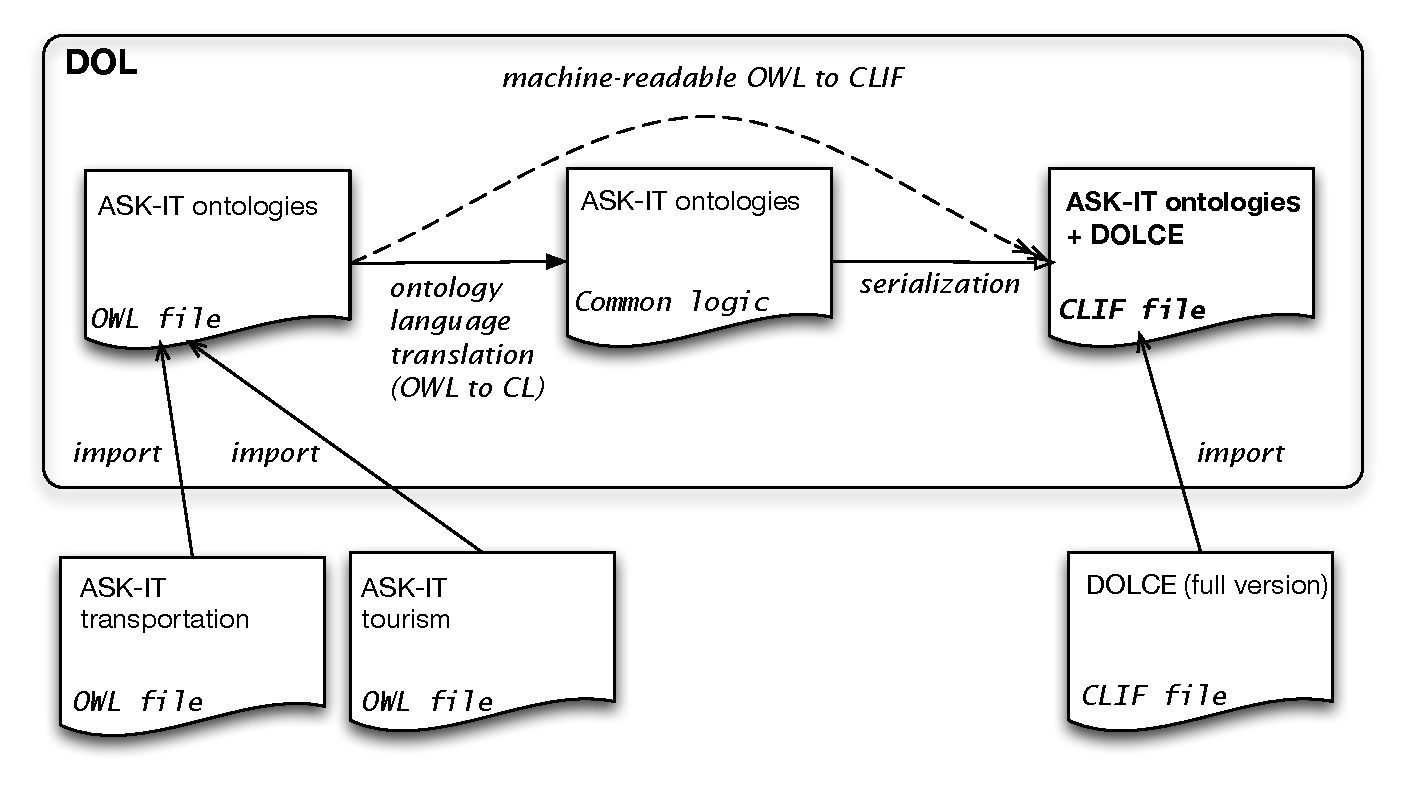
\includegraphics[width=\textwidth]{illustrations/DOLfig.pdf}
  \caption{Mapping between two OMS formulated in different OMS languages}
\label{f:DOL-mapping}
\end{figure}

%%%%%%%%%%%%%%%%%%%%%%%%%%%%%%%%%%%%%%%%%%%%%%%%%%%%%%%%%%%%%%%%%%%%%%%%%%%%%%%%%%%%%%%%%%%%%%%%%%%%%%%%%%%%%%%%%%%%%%%%%%%%%%%%%%
%%%%%%%%%%%%%%%%%%%%%%%%%%%%%%%%%%%%%%%%%%%%%%%%%%%%%%%%%%%%%%%%%%%%%%%%%%%%%%%%%%%%%%%%%%%%%%%%%%%%%%%%%%%%%%%%%%%%%%%%%%%%%%%%%%

\sclause{\DOL Provides a Mechanism for Rich Annotation and Documentation of OMS}\label{c:req:annotation}

\DOL provides a mechanism for identifying anything of relevance in OMS by assigning an IRI to it.  With RDF there is a standard mechanism for annotating things identified by IRIs.  Thus, \DOL supports  annotations in the full generality specified in \cref{c:terms-annotation}.

%A list of recommended RDF vocabularies for annotating OMS is presented in annex \ref{a:dol-onto}.


%%%%%%%%%%%%%%%%%%%%%%%%%%%%%%%%%%%%%%%%%%%%%%%%%%%%%%%%%%%%%%%%%%%%%%%%%%%%%%%%%%%%%%%%%%%%%%%%%%%%%%%%%%%%%%%%%%%%%%%%%%%%%%%%%%
%%%%%%%%%%%%%%%%%%%%%%%%%%%%%%%%%%%%%%%%%%%%%%%%%%%%%%%%%%%%%%%%%%%%%%%%%%%%%%%%%%%%%%%%%%%%%%%%%%%%%%%%%%%%%%%%%%%%%%%%%%%%%%%%%%
%%%%%%%%%%%%%%%%%%%%%%%%%%%%%%%%%%%%%%%%%%%%%%%%%%%%%%%%%%%%%%%%%%%%%%%%%%%%%%%%%%%%%%%%%%%%%%%%%%%%%%%%%%%%%%%%%%%%%%%%%%%%%%%%%%

\cleardoublepage
\clause{\DOL  Syntax}\label{c:abstract-syntax}%\label{a:text-syntax}
\sclause{General}

This clause specifies the \DOL abstract syntax as a MOF \nref{MOF} metamodel.
In annex~\ref{a:EBNF}, the same abstract syntax is specified using EBNF.
We further include  the \DOL concrete syntax, which
uses the metaclasses of the abstract syntax as non-terminals of
an EBNF grammar.


At several places, the concrete syntax uses the non-terminal
\syntax{'end'} to mark the end of a definition or declaration. Tools
may make this \syntax{'end'} optional. However, in this standard,
the \syntax{'end'} is not marked as optional, because it may be needed to effectively
disambiguate heterogeneous texts.

The concrete syntax in EBNF relates to the abstract syntax in MOF via a simple scheme. Each 
 non-terminal in the EBNF conforms to either a class or an attribute of a class in MOF.
By default non-terminals are represented as classes. Non-terminals are represented as attributes in MOF 
only if in the corresponding EBNF production rule a non-terminal (a) produces 
a single non-terminal  (e.g. IRI or String) and  
(b) is  not part of an alternative in another rule. 
Each generalization in MOF yields a EBNF rule that 
consists solely of alternatives of single non-terminals. 
The properties of a MOF class form a ENBF rule for the corresponding non-terminal, 
which produces the concatenation of the property types of the class with syntactic terminals.
Cardinality  `0..1' in MOF is  represented as options in EBNF.  Analogously, the cardinality 
`0..*' in MOF is represented by the repetition symbol `*' in EBNF.

\medskip
The \DOL document types are as follows
		\begin{description}
			\item[MIME type] \mimetype{application/dol+text}
			\item[Filename extension] .dol
		\end{description}

%%%%%%%%%%%%%%%%%%%%%%%%%%%%%%%%%%%%%%%%%%%%%%%%%%%%%%%%%%%%%%%%%%%%%%%%%%%%%%%%%%%%%%%%%%%%%%%%%%%%%%%%%%%%%%%%%%%%%%%%%%%%%%%%%%
%%%%%%%%%%%%%%%%%%%%%%%%%%%%%%%%%%%%%%%%%%%%%%%%%%%%%%%%%%%%%%%%%%%%%%%%%%%%%%%%%%%%%%%%%%%%%%%%%%%%%%%%%%%%%%%%%%%%%%%%%%%%%%%%%%

\sclause{MOF Metaclasses}
\label{s:mof-metaclasses}

\DOL provides MOF metaclasses for (among others):   
\begin{itemize}
\item OMS (which can be native OMS in some OMS language, or unions, translations,  closures, combinations, approximations of OMS, among others)
\item OMS mappings 
\item OMS networks
%\item \red{queries}
\item \DOL libraries (items in these are: definitions of OMS, OMS mappings, and OMS networks, as well as qualifications choosing (1) the logic,
(2) the OMS language and/or (3) the serialization)
\item identifiers
\item annotations
\end{itemize}
 
The \DOL metaclasses \syntax{NativeDocument} and \syntax{BasicOMS} are
abstract metaclasses without any instances within the normative \DOL
metamodel.  In order to use \DOL with some specific conforming OMS language, the top-level MOF
metaclass of the abstract syntax of this language
(\cf \cref{c:conform:logic}) has to be a subclass (in the sense of
SMOF multiple classification) of the \DOL metaclass
\syntax{NativeDocument}, see Fig.~\ref{fig:native_document}. 
Likewise, if the conforming OMS language has a metaclass for basic OMS,
this has to be a subclass of the metaclass \syntax{BasicOMS},
see Fig.~\ref{fig:basic_oms}.
See the informative annexes~\ref{a:owl} to~\ref{a:casl} for details.


\begin{figure}[b]
  \centering
    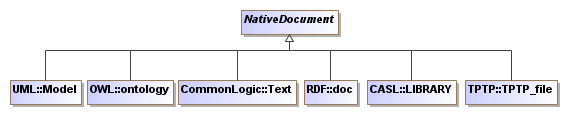
\includegraphics[scale=0.47]{mof/native_document.png}
   \caption{Informative diagram showing subclasses of \syntax{NativeDocument}}
   \label{fig:native_document}
\end{figure}


\begin{figure}
  \centering
    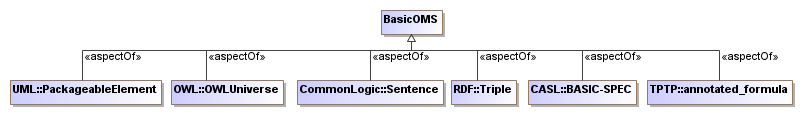
\includegraphics[scale=0.47]{mof/basic_oms.png}
   \caption{Informative diagram showing subclasses of \syntax{BasicOMS}}
   \label{fig:basic_oms}
\end{figure}

%%%%%%%%%%%%%%%%%%%%%%%%%%%%%%%%%%%%%%%%%%%%%%%%%%%%%%%%%%%%%%%%%%%%%%%%%%%%%%%%%%%%%%%%%%%%%%%%%%%%%%%%%%%%%%%%%%%%%%%%%%%%%%%%%%
%%%%%%%%%%%%%%%%%%%%%%%%%%%%%%%%%%%%%%%%%%%%%%%%%%%%%%%%%%%%%%%%%%%%%%%%%%%%%%%%%%%%%%%%%%%%%%%%%%%%%%%%%%%%%%%%%%%%%%%%%%%%%%%%%%

\sclause{Documents}\label{c:libraries}

%%%%%%%%%%%%%%%%%%%%%%%%%%%%%%%%%%%%%%%%%%%%%%%%%%%%%%%%%%%%%%%%%%%%%%%%%%%%%%%%%%%%%%%%%%%%%%%%%%%%%%%%%%%%%%%%%%%%%%%%%%%%%%%%%%

\ssclause{Abstract Syntax}

The DOL metamodel for documents and libraries is shown in Fig.~\ref{fig:libraries}.
A \termref{document} (\syntax{Document}) can be a 
\begin{itemize}
\item a \DOL library, or
\item a \syntax{NativeDocument}, which is the verbatim inclusion of an
  OMS written in an OMS language that conforms with \DOL; \cf
  \ref{c:conform:logic}).
\end{itemize}
A \DOL library consists of a collection of (named)  OMS,  OMS networks, and mappings between these.  More specifically, a \DOL
library consists of a name, followed by a list of
\syntax{LibraryItem}s.  A \syntax{LibraryItem} is either a
\syntax{Definition},
an import of another \DOL library (\syntax{LibraryImport}),
%a definition related to queries 
%(\syntax{QueryRelatedDefinition})
or a \syntax{Qualification} selecting a specific
OMS language, logic and/or syntax that is used to interpret the
subsequent \syntax{LibraryItem}s.  
 A \syntax{LibraryImport} leads to the inclusion of all \syntax{LibraryItem}s of the imported \DOL library into the importing one.
A \syntax{Definition} assigns an IRI to an OMS  (\syntax{OMSDefinition}), 
to a mapping between OMS (\syntax{MappingDefinition}), or
an OMS network  (\syntax{NetworkDefinition}). Moreover, annex~\ref{a:queries}
informatively introduces \syntax{QueryRelatedDefinition}.

At the beginning of a \DOL library, one can declare a \syntax{PrefixMap} for abbreviating long IRIs  using CURIEs; see \cref{c:identifiers} for further details. Examples of the use of \DOL library can be found in Appendix~\ref{a:uses} and Section~\ref{c:goal}.

\medskip
\begin{figure}
  \centering
    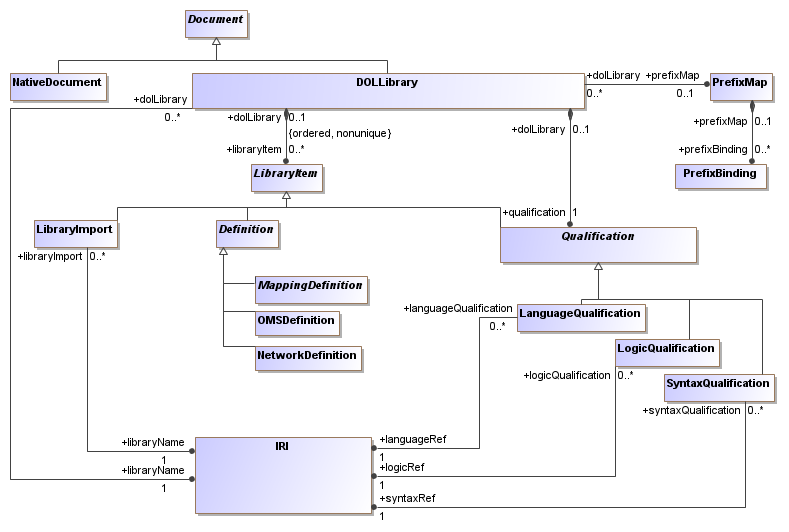
\includegraphics[scale=0.47]{mof/libraries.png}
  \caption{DOL metamodel: Documents and libraries}
  \label{fig:libraries}
\end{figure}

%%%%%%%%%%%%%%%%%%%%%%%%%%%%%%%%%%%%%%%%%%%%%%%%%%%%%%%%%%%%%%%%%%%%%%%%%%%%%%%%%%%%%%%%%%%%%%%%%%%%%%%%%%%%%%%%%%%%%%%%%%%%%%%%%%

\ssclause{Concrete Syntax}
%%%%%%%%%%%%%%%%%%%%%%%%%%%%%%%%%%%%%%%%%%%%%%%%%%%%%%%%%%%%%%%%%%%%%%%%%%%%%%%%%%%%%%%%%%%%%%%%%%%%%%%%%%%%%%%%%%%%%%%%%%%%%%%%%%
\sssclause{Documents}
\vspace{-2em}
 
\begin{lstlisting}[language=ebnf,escapeinside={@@},morecomment={[l]{\%\%\ }}]

Document           ::= DOLLibrary | NativeDocument
DOLLibrary         ::= [PrefixMap] 'library' LibraryName
                           Qualification LibraryItem*
NativeDocument     ::= @$<$\rm language and serialization specific $>$@ 
LibraryItem        ::= LibraryImport | Definition | Qualification
Definition         ::= OMSDefinition
                     | NetworkDefinition
                     | MappingDefinition
LibraryImport      ::= 'import' LibraryName
Qualification      ::= LanguageQualification
                     | LogicQualification
                     | SyntaxQualification
LanguageQualification ::= 'language' LanguageRef
LogicQualification ::= 'logic' LogicRef
SyntaxQualification ::= 'serialization' SyntaxRef
LibraryName        ::= IRI
LanguageRef        ::= IRI
LogicRef           ::= IRI
SyntaxRef          ::= IRI
\end{lstlisting}


\begin{lstlisting}[language=ebnf,escapechar=+,morecomment={[l]{\%\%\ }}]

PrefixMap      ::= '%prefix(' PrefixBinding* ')%'
PrefixBinding  ::= BoundPrefix IRIBoundToPrefix [Separators]
BoundPrefix    ::= ':' | Prefix +$<$\rm see definition in \cref{c:curies}$>$\CLnote[type=q-aut]{I think that, in contrast to OWL Manchester, we can allow prefix names that match keywords of the \DOL syntax, as we are enclosing the whole prefix map into an annotation construct -- right?}+
IRIBoundToPrefix ::= '<' FullIRI '>'
Separators     ::= 'separators' SeparatorString SeparatorString
SeparatorString ::= SeparatorChar SeparatorChar*
SeparatorChar  ::= ipchar | gen-delims - '#'+$<$\rm as defined in \nref{IRI}$>$+
\end{lstlisting}


 Note that the empty prefix (called ``no prefix'' in \nref{RDFa}, Section 6) is denoted by a colon inside the prefix map, but it is omitted in CURIEs.  This is the style of the OWL Manchester syntax \cite{W3C:NOTE-owl2-manchester-syntax-20091027} but differs from the RDFa Core 1.1 syntax.

\vspace{1em}
	


%%%%%%%%%%%%%%%%%%%%%%%%%%%%%%%%%%%%%%%%%%%%%%%%%%%%%%%%%%%%%%%%%%%%%%%%%%%%%%%%%%%%%%%%%%%%%%%%%%%%%%%%%%%%%%%%%%%%%%%%%%%%%%%%%%
%%%%%%%%%%%%%%%%%%%%%%%%%%%%%%%%%%%%%%%%%%%%%%%%%%%%%%%%%%%%%%%%%%%%%%%%%%%%%%%%%%%%%%%%%%%%%%%%%%%%%%%%%%%%%%%%%%%%%%%%%%%%%%%%%%

\sclause{OMS Networks}\label{c:networks}

%%%%%%%%%%%%%%%%%%%%%%%%%%%%%%%%%%%%%%%%%%%%%%%%%%%%%%%%%%%%%%%%%%%%%%%%%%%%%%%%%%%%%%%%%%%%%%%%%%%%%%%%%%%%%%%%%%%%%%%%%%%%%%%%%%

\ssclause{Abstract Syntax}
The DOL metamodel for documents and libraries is shown in Fig.~\ref{fig:libraries}.
Inside a \DOL library, with a \syntax{NetworkDefinition}, one can
define OMS networks (also called distributed OMS). OMS networks are
typically used for complex viewpoint specifications; they also can be
used in \syntax{combination}s (see clause~\ref{c:OMS} below). A
\syntax{NetworkDefinition} names an OMS network consisting of
\syntax{NetworkElement}s. These can be \syntax{ElementRef}s,
i.e.\ IRIs that name OMS, OMS mappings, or previously-defined OMS
networks. \syntax{ElementRef}s that are OMS can be prefixed with an
\syntax{Id}; this is then used for disambiguation in a
\syntax{combination}.  An optional \syntax{ConservativityStrength}
specifies e.g.\ consistency of the network (analogously to
\syntax{OMSDefinition}s, see clause~\ref{c:OMS} below for details).


An OMS network by default also includes all inclusions (between
the extended and the extending OMS of an \syntax{ExtensionOMS})
between the involved OMS---unless these are explicitly excluded.
The latter can be achieved using \syntax{ExcludingElement}s.
They consist of \syntax{ElementRef}s naming OMS or OMS mappings,
and of \syntax{PathReference}s. A \syntax{PathReference} refers
to an unnamed OMS mapping (e.g.\ one generated by an \syntax{Extension}) 
by specifying its source and target OMS. See Clauses~\ref{spec-2}, \ref{sec:atm-example}
and Appendix~\ref{ex:alignment} for an example network and of the use of \syntax{combination}.

\medskip
\begin{figure}
  \centering
    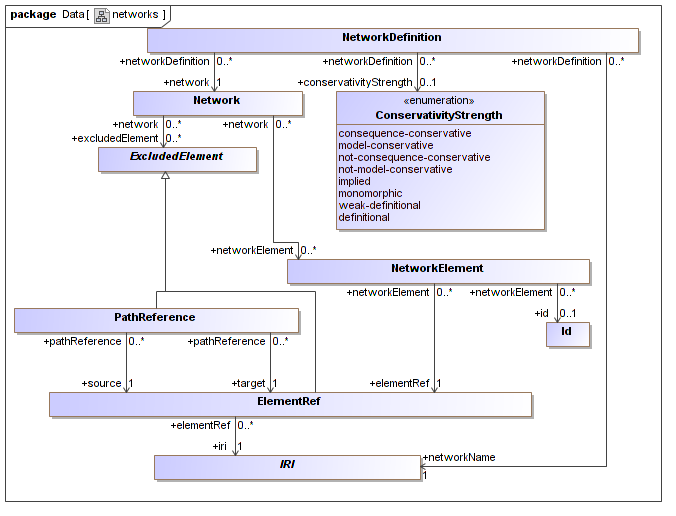
\includegraphics[scale=0.47]{mof/networks.png}
  \caption{DOL metamodel: Networks}
  \label{fig:networks}
\end{figure}


%%%%%%%%%%%%%%%%%%%%%%%%%%%%%%%%%%%%%%%%%%%%%%%%%%%%%%%%%%%%%%%%%%%%%%%%%%%%%%%%%%%%%%%%%%%%%%%%%%%%%%%%%%%%%%%%%%%%%%%%%%%%%%%%%%

\ssclause{Concrete Syntax}

\vspace{-1.4em}
\begin{lstlisting}[language=ebnf,escapeinside={@@},morecomment={[l]{\%\%\ }}]

NetworkDefinition ::= 'network' NetworkName '='
                      [ConservativityStrength] Network
NetworkName     ::= IRI
Network         ::= NetworkElements [ExcludedElements]
NetworkElements ::= NetworkElement ( ',' NetworkElement )*
NetworkElement  ::= [Id ':'] ElementRef
ExcludedElements ::= 'excluding' ExcludedElement ( ',' ExcludedElement )*
ExcludedElement ::= PathReference | ElementRef
PathReference   ::= IRI '->' IRI
ElementRef      ::= IRI
Id              ::= Letter LetterOrDigit*
\end{lstlisting}

%%%%%%%%%%%%%%%%%%%%%%%%%%%%%%%%%%%%%%%%%%%%%%%%%%%%%%%%%%%%%%%%%%%%%%%%%%%%%%%%%%%%%%%%%%%%%%%%%%%%%%%%%%%%%%%%%%%%%%%%%%%%%%%%%%
%%%%%%%%%%%%%%%%%%%%%%%%%%%%%%%%%%%%%%%%%%%%%%%%%%%%%%%%%%%%%%%%%%%%%%%%%%%%%%%%%%%%%%%%%%%%%%%%%%%%%%%%%%%%%%%%%%%%%%%%%%%%%%%%%%

\sclause{OMS}\label{c:OMS}

%%%%%%%%%%%%%%%%%%%%%%%%%%%%%%%%%%%%%%%%%%%%%%%%%%%%%%%%%%%%%%%%%%%%%%%%%%%%%%%%%%%%%%%%%%%%%%%%%%%%%%%%%%%%%%%%%%%%%%%%%%%%%%%%%%

\ssclause{Abstract Syntax}

The DOL metamodel for OMS is shown in Fig.~\ref{fig:oms}.
\DOL provides a rich structuring language for OMS, providing
extension, translation, unions of OMS and many more.  For each of
these alternatives, a subclass is introduced. An OMS can be
\begin{itemize}
\item a \syntax{TranslationOMS} involving both
an OMS (to be translated), and a specification of the translation,
which is covered by the class \syntax{OMSTranslation}
(see Appendix~\ref{dist-het-onto}, \ref{ex:DDL}, for examples);
\item a \syntax{UnionsOMS}, uniting two given OMS 
(see Appendix~\ref{ex:engine} for an example);
\item a \syntax{ClosureOMS}, applying a closure operator
(given by a \syntax{Closure}) to an OMS (see Appendix~\ref{ex:definedconcepts} and~\ref{ex:datatypes} for examples); 
\item an \syntax{ExtensionOMS}, extending a given OMS with another OMS
  (given by the \syntax{Extension}). The major difference between a
  union and extension is that the members of the unions need to be
  self-contained OMS, while the extensions may reuse the signature of
  the extended OMS
  (see Appendix~\ref{ex:engine}, \ref{dist-het-onto}, \ref{ex:definedconcepts} for examples);
\item an \syntax{ExtendingOMS}, which is a very simple form of OMS,
namely a basic OMS or an OMS reference (see below);
\item a \syntax{FilteringOMS}, applying a filtering operator
(given by a \syntax{Filtering}) to an OMS
  (see Appendix~\ref{ex:reject} for an example);
\item an \syntax{ApproximationOMS}, applying an approximation operator
(given by an \syntax{Approximation}) to an OMS (see Appendix~\ref{ex:algebra} for an example);
\item a \syntax{CombinationOMS}, giving a combination of (the OMS
  contained in) an OMS network (technically, this is a colimit, see
  \cite{ZimmermanEtAl06}) 
  (see Appendix~\ref{ex:alignment} for an example of the use of \syntax{combination});
\item a \syntax{ReductionOMS}, applying a reduction
(given by an \syntax{Reduction}) to an OMS (see use cases~\ref{spec-1}, \ref{spec-2} and~\ref{model-1} and Appendix~\ref{ex:algebra} and~\ref{ex:metric-spaces} for examples);
\item a \syntax{ExtractionOMS}, applying a module extraction operator
(given by an \syntax{Extraction}) to an OMS
 (see use case \ref{onto-3} for an example);
\item a \syntax{QualifiedOMS}, which is an OMS qualified with the OMS
  language that is used to express it.
\end{itemize}
Moreover, annex~\ref{a:queries}
informatively introduces \syntax{Application}s, which apply a substitution
to an OMS.

A \syntax{ConservativityStrength} specifies additional relations that
may hold between an OMS and its extension (or union with other OMS),
like conservative or definitional extension. The rationale is that the
extension should not have impact on the original OMS that is being
extended. 

An OMS definition \syntax{OMSDefinition} names an OMS.  It can be
optionally marked as inconsistent, consistent, monomorphic or having a
unique realisation using \syntax{ConservativityStrength}. More precisely,
\syntax{'consequence-conservative'} here requires the OMS to have only
tautologies as signature-free logical consequences, while
\syntax{'not\-consequence-conservative'} expresses that this is not
the case.  \syntax{'model-conservative'} requires satisfiability of
the OMS, \syntax{'not-model-conservative'} its unsatisfiability.
\syntax{'de\-fi\-nitional'} expresses that the OMS has a unique
realisation (see Appendix~\ref{ex:definedconcepts} for an example); this may be interesting for characterizing OMS
(e.g.\ returned by model finders) that are used to describe single
realisations.



\begin{figure}
  \centering

    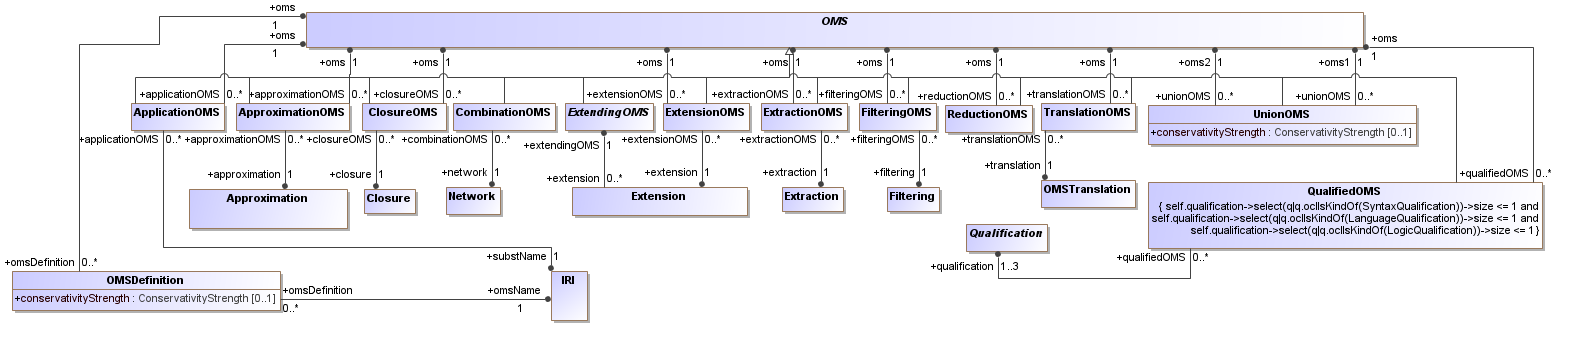
\includegraphics[scale=0.43]{mof/oms.png}
  \caption{DOL metamodel: OMS}
  \label{fig:oms}
  	
\end{figure}




The DOL metamodel for extension OMS is shown in Fig.~\ref{fig:extension&closure}.
\syntax{ExtendingOMS} is a subclass of \syntax{OMS}, containing
those OMS that may be used to extend a given OMS within an \syntax{ExtensionOMS}.
An \syntax{ExtendingOMS} can be one of the following:
\begin{itemize}
\item a basic OMS \syntax{BasicOMS} written inline, in a conforming serialization of a conforming OMS 
language (which is defined outside this standard; practically every example uses basic OMS)\footnote{In this place, any OMS in a conforming serialization of a conforming OMS language is permitted.  
However, \DOL's module sublanguage should be used instead of the module sublanguage of 
the respective conforming OMS language; \eg \DOL's OMS reference and extension construct should be preferred over OWL's import construct.}.
Note that a basic OMS used inside a DOL document may not use any of the DOL
keywords (see clause~\ref{c:keywords}); otherwise, it needs to be enclosed in curly braces\footnote{This restriction applies to DOL documents only,
 not to native documents.};
\item a reference (through an IRI) to an OMS (\syntax{OMSReference}, many examples illustrate this); or
\item a \syntax{RelativeClosureOMS}, applying a closure operator to a
  basic OMS or OMS reference (these two are hence joined into
  \syntax{ClosableOMS}). A closure forces the subsequently declared
  non-logical symbols to be interpreted in a minimal  or
  maximal way, while the non-logical symbols declared  in
  the local environment are fixed.\footnote
  {Note that if applied to algebraic signatures (sorts and operation symbols),
    minimization can be used to express reachability (i.e. term-generatedness)
    of algebraic (first-order) models.}
  Variants of closure are
  minimization, maximization, freeness (minimizing also data
  sets and equalities on these,  which enables the inductive
  definition of relations and datatypes), and cofreeness (enabling the
  coinductive definition of relations and datatypes).
  See Annex~\ref{ex:blocks} for examples of the former two, and
  Annex~\ref{ex:datatypes} for examples of the latter two.
\end{itemize}
Recall that the local environment is the OMS built from all
previously-declared symbols and axioms.

Using \syntax{ExtendingOMS}, extensions of an OMS with an \syntax{ExtendingOMS}
can be built. The latter can optionally be named and/or marked as conservative, monomorphic, definitional, weakly definitional or implied (using a \syntax{ConservativityStrength}, see clause~\ref{s:structuredOMS} for details).
Note that an \syntax{ExtendingOMS} used in an extension must
not be an \syntax{OMSReference}.

\medskip
\begin{figure}
  \centering
    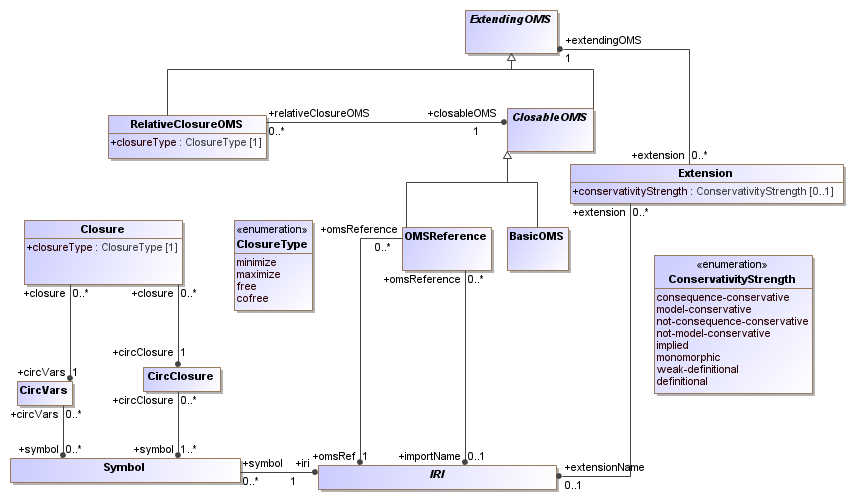
\includegraphics[scale=0.47]{mof/extension&closure.png}
  \caption{DOL metamodel: Extension and closure OMS}
  \label{fig:extension&closure}
\end{figure}


Furthermore, OMS can be constructed using 
\begin{itemize}
\item  closures of an OMS with a \syntax{Closure}.  This is
  similar to a \syntax{RelativeClosureOMS}, but the non-logical
  symbols to be  minimized/maximized and to be varied are
  explicitly declared here (while a \syntax{RelativeClosureOMS} takes
  the local environment to be fixed, i.e.\ not varied);
\item a translation \syntax{OMSTranslation} of an OMS into a different
  signature or OMS language. The former is done using a \syntax{SymbolMap},
  specifying a map of symbols to symbols. The latter is done using an 
  OMS language
  translation \syntax{OMSLanguageTranslation} can be either specified
  by its name, or be inferred as the \termref{default translation} to
  a given target (the source will be inferred as the OMS language of
  the current OMS);
\item a \syntax{Reduction} of an OMS to a smaller signature and/or
  less expressive logic (that is, some non-logical symbols and/or some
  parts of the structure of the realisation are hidden, 
  but the semantic effect of
  sentences involving these is kept). The former is done using a
  \syntax{SymbolList}, which is a list of non-logical symbols that are
  to be hidden. The latter uses an \syntax{OMSLanguageTranslation}
  denoting a logic projection that is used as logic reduction to a
  less expressive OMS language.
\item an \syntax{Approximation} of an OMS, in a subsignature (\syntax{InterfaceSignature}) or sublogic, with the effect that sentences not expressible in the subsignature respectively sublogic are replaced with a suitable approximation,
\item a \syntax{Filtering} of an OMS, with the effect that some signature symbols and axioms (specified by a \syntax{BasicOMS}) are removed from the OMS,
\item a module \syntax{Extraction} of an OMS, using a restriction signature (\syntax{InterfaceSignature}).
\end{itemize}
In all of these cases except for translation, a \syntax{RemovalKind}
specifies whether the listed symbols are removed from the OMS, or
whether they are kept (and the other ones are removed).

The DOL metamodel for closure OMS is shown in
Fig.~\ref{fig:extension&closure}, that for translation and reduction
OMS in Fig.~\ref{fig:translations&reduction}. 



\medskip
\begin{figure}
  \centering
    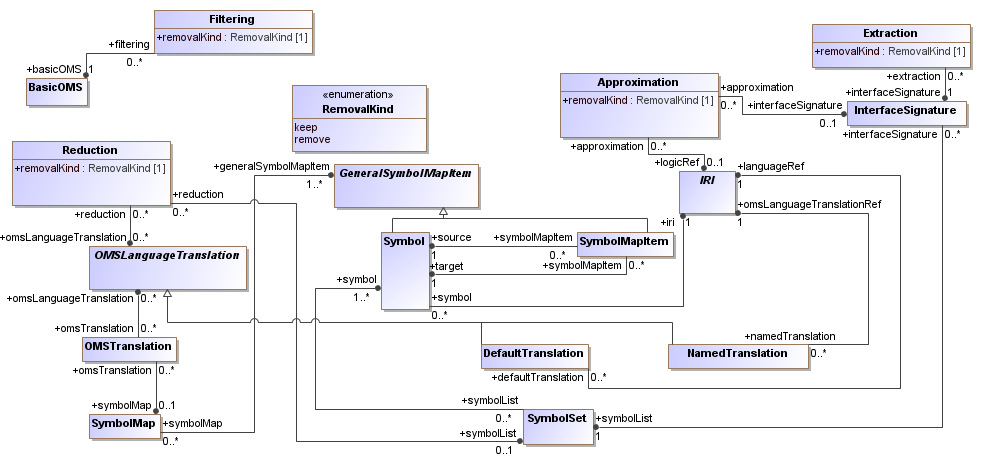
\includegraphics[scale=0.47]{mof/translation&reduction.png}
  \caption{DOL metamodel: Translation and reduction OMS}
  \label{fig:translations&reduction}
\end{figure}

%% \CLnote[type=fyi]{On 2012-07-18 we decided 
%% not to specify lambda-style symbol-to-term mappings for now.  Would be convenient, but specifying its semantics 
%% in an OMS language independent way would require additional institution infrastructure – and the same effect can be 
%% achieved by auxiliary definitional extensions, cf.\ Colore (so promote this, informatively, as a ``best practice''?) TM: Alternatively, we could use a recent notion of institutional monad. This builds an extended signature with all terms. Then one can use ordinary signature morphisms into such extended signatures.} 
%or a logic
%translation. 

%%%%%%%%%%%%%%%%%%%%%%%%%%%%%%%%%%%%%%%%%%%%%%%%%%%%%%%%%%%%%%%%%%%%%%%%%%%%%%%%%%%%%%%%%%%%%%%%%%%%%%%%%%%%%%%%%%%%%%%%%%%%%%%%%%

\ssclause{Concrete Syntax} \label{a:dol-text:OMS}


While in most cases the translation from concrete to abstract syntax
is obvious (the structure is largely the same),  
\begin{itemize}
\item both \syntax{\%satisfiable}, \syntax{\%cons} and \syntax{\%mcons} are translated
  to \syntax{model-conservative},
\item both \syntax{\%consistent}  and \syntax{\%ccons} are translated
  to \syntax{consequence-conservative},
\item  both   \syntax{\%unsatisfiable} and \syntax{\%notmcons} are translated to
  \syntax{not-model-conservative},
\item both \syntax{\%inconsistent}  and \syntax{\%notccons} are translated
  to \syntax{not-consequence-conservative},
\item moreover, both \syntax{closed-world} and \syntax{minimize} are
  translated to \syntax{minimize}.
\end{itemize}
Note that the MOF abstract syntax subsumes all these elements except
from those in the last line under the enumeration class
\syntax{ConservativityStrength}. Not all elements of the enumeration
can be used at any position; the corresponding restrictions are
expressed as OCL constraints.  By contrast, the concrete syntax
features a more fine-grained structure of non-terminals
(\syntax{Conservative}, \syntax{ConservativityStrength} and
\syntax{ExtConservativityStrength}) in order to express the same
constraints via the EBNF grammar.
                       
\begin{lstlisting}[language=ebnf,escapeinside={@@},mathescape]
BasicOMS           ::= @$<$@language and serialization specific@$>$@ 
ClosableOMS        ::= BasicOMS | '{' BasicOMS '}' | OMSRef [ImportName]
ExtendingOMS       ::= ClosableOMS | RelativeClosureOMS
RelativeClosureOMS ::= ClosureType '{' ClosableOMS '}'
OMS                ::= ExtendingOMS
                     | OMS Closure
                     | OMS OMSTranslation
                     | OMS Reduction
                     | OMS Extraction
                     | OMS Approximation
                     | OMS Filtering
                     | OMS 'and' [ConservativityStrength] OMS
                     | OMS 'then' ExtensionOMS
                     | Qualification* ':' GroupOMS
                     | 'combine' NetworkElements [ExcludeExtensions]
                     | GroupOMS
Closure            ::= ClosureType CircMin [CircVars]
ClosureType        ::= 'minimize'
                     | 'closed-world'
                     | 'maximize'
                     | 'free'
                     | 'cofree'
CircMin            ::= Symbol Symbol*
CircVars           ::= 'vars' (Symbol Symbol*)
GroupOMS           ::= '{' OMS '}' | OMSRef
OMSTranslation     ::= 'with' LanguageTranslation* SymbolMap
                     | 'with' LanguageTranslation+
LanguageTranslation ::= 'translation' OMSLanguageTranslation
Reduction          ::= 'hide' LogicReduction* SymbolList
                     | 'hide' LogicReduction+
                     | 'reveal' SymbolList
LogicReduction     ::= 'along' OMSLanguageTranslation
SymbolList         ::= Symbol ( ',' Symbol )*
SymbolMap          ::= GeneralSymbolMapItem ( ',' GeneralSymbolMapItem )*
Extraction         ::= 'extract' InterfaceSignature
                     | 'remove' InterfaceSignature
Approximation      ::= 'forget' InterfaceSignature ['keep' LogicRef]
                     | 'keep' InterfaceSignature ['keep' LogicRef]
                     | 'keep' LogicRef
Filtering          ::= RemovalKind BasicOMSOrSymbolList
RemovalKind        ::= 'reject' | 'select'
BasicOMSOrSymbolList ::= '{' BasicOMS '}' | SymbolList
ExtensionOMS       ::= [ExtConservativityStrength]
                       [ExtensionName]
                       ExtendingOMS
ConservativityStrength ::= Conservative | '%mono' | '%wdef' | '%def'
ExtConservativityStrength ::= ConservativityStrength | '%implied'
Conservative       ::= '%cons'
                     | '%ccons'
                     | '%mcons'
                     | '%notccons'
                     | '%notmcons'
                     | '%consistent'
                     | '%inconsistent'
                     | '%satisfiable'
                     | '%unsatisfiable'
InterfaceSignature ::= SymbolList
ImportName         ::= '%(' IRI ')%'
ExtensionName      ::= '%(' IRI ')%'
OMSkeyword         ::= 'ontology'
                     | 'onto'
                     | 'specification'
                     | 'spec'
                     | 'model'
                     | 'oms'
OMSDefinition      ::= OMSkeyword OMSName '='
                       [ConservativityStrength] OMS 'end'
Symbol             ::= IRI
SymbolMapItem      ::= Symbol '|->' Symbol
GeneralSymbolMapItem ::= Symbol | SymbolMapItem
Sentence           ::= @$<$@an expression specific to an OMS language@$>$@ 
OMSName            ::= IRI
OMSRef             ::= IRI
LoLaRef            ::= LanguageRef | LogicRef
\end{lstlisting}


\begin{lstlisting}[language=ebnf,mathescape]

OMSLanguageTranslation ::= OMSLanguageTranslationRef | '->' LoLaRef
OMSLanguageTranslationRef ::= IRI
\end{lstlisting}


%\ednote{\%safe is more a statement about an import of a module, 
%and hence should be a statement in an OMS network. Recall:
%ModuleProperties     =  '\%safe' ; }

The above grammar allows for some grouping ambiguity when using operators in
OMS definitions. These ambiguities are resolved according to the following
list, listing operators in decreasing order of precedence:
\begin{itemize}
  \item \syntax{minimize}, \syntax{maximize}, \syntax{free}, and \syntax{cofree}. 
  \item \syntax{extract}, \syntax{forget}, \syntax{hide}, \syntax{keep},
    \syntax{reject}, \syntax{remove}, \syntax{reveal}, \syntax{select}, and
    \syntax{with}.
  \item \syntax{and}.
  \item \syntax{then}.
\end{itemize}
Multiple occurrences of the same operator are grouped in a left associative
manner. In all other cases operators on the same precedence level are not
implicitly grouped and have to be grouped explicitly. Omitting such an explicit
grouping results in a parse error.

%%%%%%%%%%%%%%%%%%%%%%%%%%%%%%%%%%%%%%%%%%%%%%%%%%%%%%%%%%%%%%%%%%%%%%%%%%%%%%%%%%%%%%%%%%%%%%%%%%%%%%%%%%%%%%%%%%%%%%%%%%%%%%%%%%
%%%%%%%%%%%%%%%%%%%%%%%%%%%%%%%%%%%%%%%%%%%%%%%%%%%%%%%%%%%%%%%%%%%%%%%%%%%%%%%%%%%%%%%%%%%%%%%%%%%%%%%%%%%%%%%%%%%%%%%%%%%%%%%%%%

\sclause{OMS Mappings}\label{c:oms-mappings}

%%%%%%%%%%%%%%%%%%%%%%%%%%%%%%%%%%%%%%%%%%%%%%%%%%%%%%%%%%%%%%%%%%%%%%%%%%%%%%%%%%%%%%%%%%%%%%%%%%%%%%%%%%%%%%%%%%%%%%%%%%%%%%%%%%

\ssclause{Abstract Syntax}


An OMS mapping provides a connection between two OMS. An OMS mapping
definition is the definition of either a named interpretation
(\syntax{InterpretationDefinition}, see Annex~\ref{ex:engine} for an example), entailment (\syntax{EntailmentDefinition}, see use case~\ref{sec:atm-example} for an example),
refinement (\syntax{RefinementDefinition}, see use cases~\ref{spec-2} and~\ref{sec:atm-example} for examples) or equivalence
(\syntax{EquivalenceDefinition}, see Annex~\ref{ex:engine} for an example), a named declaration of the relation
between a module of an OMS and the whole OMS
(\syntax{ConservativeExtensionDefinition}, see use case~\ref{onto-3} for an example), or a named \termref{alignment}
(\syntax{AlignmentDefinition}, see use case~\ref{onto-2} and Annex~\ref{ex:alignment} for examples).


The DOL metamodel for  interpretations and refinements is shown in 
Fig.~\ref{fig:interpretations&refinements}.
Both interpretations and refinements specify a logical entailment or
specialization relation between OMS.\\
 An
\syntax{InterpretationDefinition} specifies source and target OMS
(forming the \syntax{InterpretationType}), as well as a
\syntax{SymbolMap} and/or an \syntax{OMSLanguageTranslation}.  The
\syntax{SymbolMap} in an interpretation always must lead to a
signature morphism. A proof obligation expressing that the source OMS,
when translated along the signature morphism and/or the
\syntax{OMSLanguageTranslation}, logically follows from the target OMS.

A symbol map in an interpretation is \required to cover all
non-logical symbols of the source OMS; the semantics specification in
\cref{c:semantics} makes this assumption. ({Mapping a non-logical
  symbol twice is an error. Mapping two source non-logical symbols to
  the same target non-logical symbol is legal, this is a non-injective
  OMS mapping.})

\syntax{Refinement}s subsume interpretations (via
\syntax{SimpleRefinement}s), but allow the specification of much more
complex relation between OMS (and OMS networks).  The style differs
from interpretation in that even a single OMS is a refinement (via
\syntax{RefinementOMS}); this corresponds to the source of an
interpretation. Using \syntax{SimpleOMSRefinement}s, a refinement can
be further specialized to a (target) OMS via an
\syntax{OMSRefinementMap}. The latter involves a symbol map and/or OMS
language translation, analogously to interpretations.  With this style
of notation, simple refinements can be easily chained up (which cannot
be done using interpretations).  Refinements themselves can
also be refined, also by other refinements---this amounts
to the possibility of composing refinements. Furthermore,
refinements can also be specified between networks
(\syntax{SimpleNetworkRefinement}, see use case~\ref{spec-2} for an example).  
A refinement between OMS networks
consists of a list of ordinary refinements (between OMS), one for
each node in the source network (the OMS refinement is then required
to refine the node in the source network to some node in the target
network). The list may also include network refinements, much in the
same way as network definitions also may include other networks.
All the ordinary refinements occuring as components of the
network refinement have to be compatible in a sense exemplified
at the end of clause~\ref{spec-2}.

\medskip
\begin{figure}
  \centering
    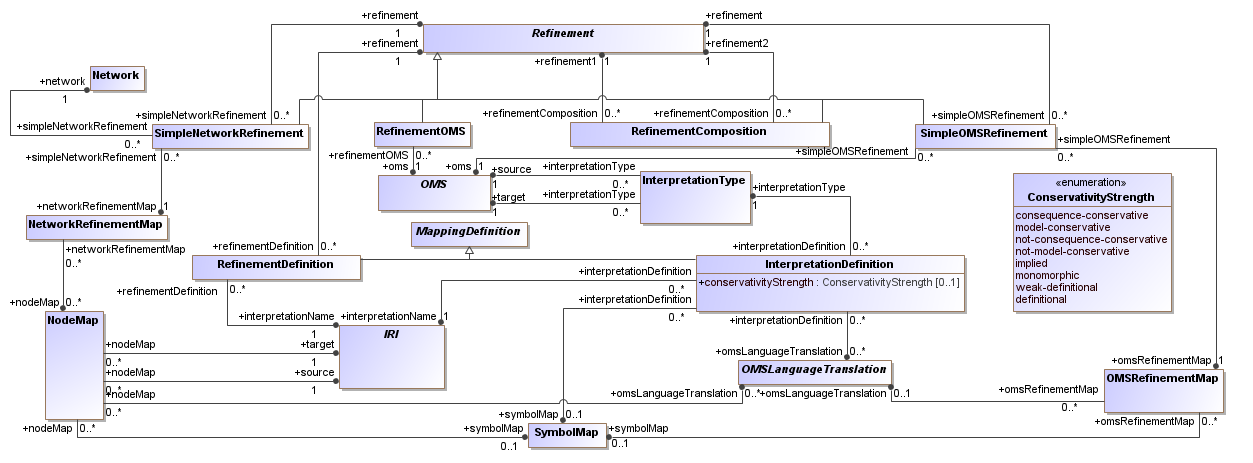
\includegraphics[scale=0.42]{mof/interpretations&refinements.png}
  \caption{DOL metamodel: Interpretations and refinements}
  \label{fig:interpretations&refinements}
\end{figure}

The DOL metamodel for entailments and equivalences is shown in 
Fig.~\ref{fig:entailment&equivalence}.
An entailment is a variant of an interpretation where all symbols are
mapped identically, while an equivalence states that the classes of realisations
of two OMS are in bijective correspondence. As for refinements,
entailments and equivalences are also possible between networks
(\syntax{NetworkNetworkEntailment} and \syntax{NetworkEquivalence}).
An entailment between a network as premise and an OMS as conclusion
(\syntax{NetworkOMSEntailment}) specifies that all realisations of the
network, when restricted to a given node (given by an IRI), are
realisations of the OMS.

\begin{figure}
  \centering
    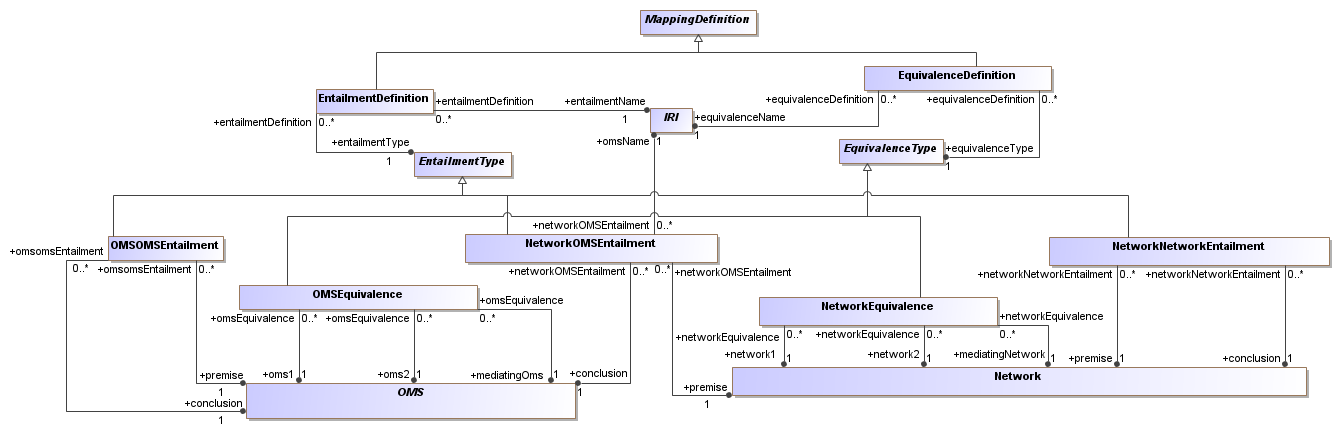
\includegraphics[scale=0.39]{mof/entailment&equivalence.png}
  \caption{DOL metamodel: Entailments and equivalences}
  \label{fig:entailment&equivalence}
\end{figure}


The DOL metamodel for alignments is shown in 
Fig.~\ref{fig:alignment}.
Signature morphisms used in interpretations and refinements use
a functional style of mapping symbols of OMS.
In contrast to this style, an alignment provides a relational 
connection between two OMS,  using a set of \syntax{Correspondence}s. Each correspondence may relate 
some OMS non-logical symbol to another one (possibly given by a term) with an optional confidence 
value. Moreover, the relation between the two non-logical symbols can be explicitly
specified (like being equal, or only being subsumed) in a similar way to the Alignment API \cite{AlignmentAPI}. 
The relations that can be used in a correspondence are equivalence, disjointness, subsumption, membership (the last two with a
variant for each direction) or a user-defined relation that is stored in a registry and must be prefixed with
\url{http://www.omg.org/spec/DOL/correspondences/}.
A default correspondence can be used; it is applied to all pairs of non-logical symbols with 
the same local names. The default relation in a correspondence is equivalence, unless  a different 
relation is specified in a surrounding 
'CorrespondenceBlock'.
Using an \syntax{AlignmentCardinality}, left and right injectivity and totality of the
\termref{alignment} can be specified (the default is left-injective, right-injective, left-total  and right-total).
With \syntax{AlignmentSemantics}, different styles of networks of aligned ontologies (to be interpreted in 
a logic-specific way) of alignments can be specified: whether a single domain is assumed, all domains are embedded into a global domain,
or whether several local domains are linked (``contextualized'') by relations.

\begin{figure}
  \centering
    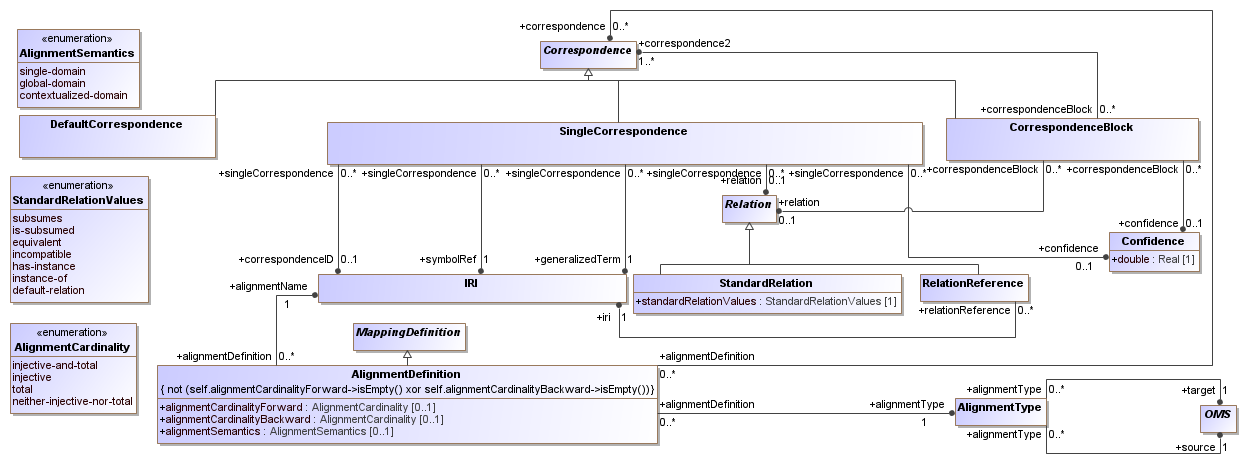
\includegraphics[scale=0.43]{mof/alignment.png}
  \caption{DOL metamodel: Alignments}
  \label{fig:alignment}
\end{figure}


The DOL metamodel for conservative extension definitions is shown in 
Fig.~\ref{fig:modules}.
A \syntax{ConservativeExtensionDefinition} declares that a certain (``whole) OMS
actually is a conservative extension some other (``module'') OMS with respect
to the \syntax{InterfaceSignature}.


\begin{figure}
  \centering
    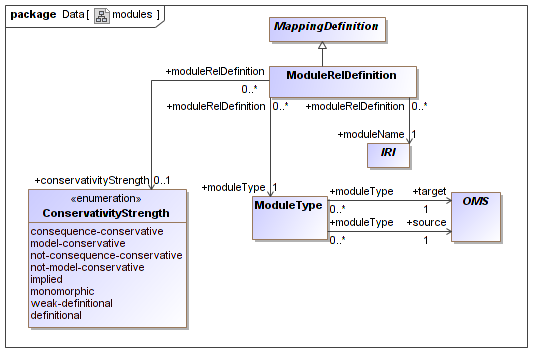
\includegraphics[scale=0.47]{mof/modules.png}
  \caption{DOL metamodel: Conservative extension definitions}
  \label{fig:modules}
\end{figure}


%%%%%%%%%%%%%%%%%%%%%%%%%%%%%%%%%%%%%%%%%%%%%%%%%%%%%%%%%%%%%%%%%%%%%%%%%%%%%%%%%%%%%%%%%%%%%%%%%%%%%%%%%%%%%%%%%%%%%%%%%%%%%%%%%%
%%%%%%%%%%%%%%%%%%%%%%%%%%%%%%%%%%%%%%%%%%%%%%%%%%%%%%%%%%%%%%%%%%%%%%%%%%%%%%%%%%%%%%%%%%%%%%%%%%%%%%%%%%%%%%%%%%%%%%%%%%%%%%%%%%

\ssclause{Concrete Syntax}\label{a:dol-text:mappings}

\vspace{-2em}
\index{alignment}
\begin{lstlisting}[language=ebnf,mathescape,escapeinside={*@}{@*}]

MappingDefinition  ::= InterpretationDefinition
                     | EntailmentDefinition
                     | EquivalenceDefinition
                     | ConservativeExtensionDefinition
                     | AlignmentDefinition
InterpretationDefinition ::= InlineInterpretation | RefinementDefinition
InlineInterpretation ::= InterpretationKeyword InterpretationName
                         [Conservative] ':' InterpretationType
                         [ '=' LanguageTranslation* [SymbolMap] ]
                         'end'
RefinementDefinition ::= InterpretationKeyword InterpretationName '='
                         Refinement
                         'end'
InterpretationKeyword ::= 'interpretation' | 'view' | 'refinement'
InterpretationName ::= IRI
InterpretationType ::= GroupOMS 'to' GroupOMS
Refinement         ::= GroupOMS
                     | NetworkName
                     | Refinement 'refined' [RefMap] 'to' Refinement
                     | Refinement 'interpreted' [RefMap] 'by' Refinement
RefMap             ::= 'via' ( OMSRefinementMap | NetworkRefinementMap )
OMSRefinementMap   ::= LanguageTranslation [SymbolMap]
                     | [LanguageTranslation] SymbolMap
NetworkRefinementMap ::= Refinement ( ',' Refinement )*
EntailmentDefinition ::= 'entailment' EntailmentName '='
                         EntailmentType 'end'
EntailmentName     ::= IRI
EntailmentType     ::= OMSOMSEntailment
                     | NetworkOMSEntailment
                     | NetworkNetworkEntailment
OMSOMSEntailment         ::= GroupOMS 'entails' GroupOMS
NetworkOMSEntailment     ::= OMSName 'in' Network 'entails' GroupOMS
NetworkNetworkEntailment ::= Network 'entails' Network
EquivalenceDefinition    ::= 'equivalence' EquivalenceName ':'
                             EquivalenceType 'end'
EquivalenceName    ::= IRI
EquivalenceType    ::= OMSEquivalence | NetworkEquivalence
OMSEquivlence      ::= GroupOMS '<->' GroupOMS ['=' OMS]
NetworkEquivalence ::= Network '<->' Network ['=' Network]
ConservativeExtensionDefinition ::= 'cons-ext' ConservativeExtensionName [Conservative] ':'
                        ConservativeExtensionType 'for' InterfaceSignature
ConservativeExtensionName       ::= IRI
ConservativeExtensionType       ::= GroupOMS 'of' GroupOMS
AlignmentDefinition ::= 'alignment' AlignmentName
                        [AlignmentCardinality AlignmentCardinality] ':'
                        AlignmentType
                        ['=' Correspondence ( ',' Correspondence )*]
                        ['assuming' AlignmentSemantics] 'end'
AlignmentName      ::= IRI
AlignmentCardinality ::= '1' | '?' | '+' | '*'
AlignmentType      ::= GroupOMS 'to' GroupOMS
AlignmentSemantics ::= 'SingleDomain'
                     | 'GlobalDomain'
                     | 'ContextualizedDomain'
Correspondence     ::= CorrespondenceBlock | SingleCorrespondence | DefaultCorrespondence
DefaultCorrespondence ::= '*' 
CorrespondenceBlock ::= 'relation' [Relation] [Confidence] '{'
                        Correspondence ( ',' Correspondence )* '}'
SingleCorrespondence ::= Symbol [Relation] [Confidence]
                         GeneralizedTerm [CorrespondenceId]
CorrespondenceId   ::= '%(' IRI ')%'
Symbol          ::= IRI
GeneralizedTerm    ::= Symbol
Relation           ::= RelationReference | StandardRelation
RelationReference  ::= IRI
StandardRelation   ::= '>' | '<' | '=' | '%' | 'ni' | 'in'
                       *@$<$ \rm No keyword corresponding to @*default-relation*@ \rm as this is just the default if@*
                       *@\phantom{$<$ }@*Relation*@ \rm is omitted $>$@*
Confidence         ::= Double
Double             ::= *@$<$ a number $\in [0,1]$ $>$@*
\end{lstlisting}

%~\CLnote{some text that was left over here, but I don't recall what we meant by it: recommendations for dealing with OMS language dialects}


%%%%%%%%%%%%%%%%%%%%%%%%%%%%%%%%%%%%%%%%%%%%%%%%%%%%%%%%%%%%%%%%%%%%%%%%%%%%%%%%%%%%%%%%%%%%%%%%%%%%%%%%%%%%%%%%%%%%%%%%%%%%%%%%%%
%%%%%%%%%%%%%%%%%%%%%%%%%%%%%%%%%%%%%%%%%%%%%%%%%%%%%%%%%%%%%%%%%%%%%%%%%%%%%%%%%%%%%%%%%%%%%%%%%%%%%%%%%%%%%%%%%%%%%%%%%%%%%%%%%%

\sclause{Identifiers}\label{c:identifiers}
This section specifies the abstract syntax of identifiers of \DOL OMS and their elements. Further, 
it introduces the concrete syntax that is used in the \DOL serialization. 
\ssclause{IRIs}\label{c:iris}


In accordance with best practices for publishing OMS on the Web, identifiers of OMS and their 
elements \should not just serve as \emph{names}, but also as \emph{locators}, which, when 
dereferenced, give access to a concrete representation of an OMS or one of its elements.  (For the 
specific case of RDF Schema and OWL OMS, these best practices are documented in 
\cite{W3C:NOTE-swbp-vocab-pub-20080828}.  The latter is a specialization of the linked data 
principles, which apply to any machine-processable data published on the Web 
\cite{BernersLee:LinkedData2006}.)  It is recommended that publicly accessible \DOL OMS be published 
as linked data.

%\todonote[type=q-aut,author=Christoph Lange]{Does this motivation/justification sound reasonable to 
%you? --- Yes.}
Therefore, in order to impose fewer conformance requirements on applications, \DOL requires the use of
 IRIs for identification per \nref{IRI}.
  It is \recommended that \DOL libraries use 
IRIs that translate to URLs when applying the algorithm for mapping IRIs to URIs specified in 
\nref{IRI}, Section 3.1.  \DOL descriptions of any element of a \DOL library that is 
identified by a certain IRI \should be \emph{located} at the corresponding URL, so that agents can 
locate them.  As IRIs are specified with a concrete syntax only in \nref{IRI}, \DOL 
adopts the latter into its abstract syntax as well as all of its concrete syntaxes 
(serializations).
The DOL metamodel for IRIs and prefixes is shown in Fig.~\ref{fig:prefixes}.

%\CLnote[type=q-all]{I meant to say: for IRIs, the abstract syntax is the same as 
%the concrete syntax.}.

%% We don't do "semantic namespaces" for now.  (Agreed in 2012-02-23 meeting)
% For identification, \DOL preferably employs IRIs that have the following three components:\footnote{This IRI syntax has originally been designed by Florian Rabe and Michael Kohlhase \cite{Rabe:MMT2011}, independently from this \IS.\todonote[type=todo,author=Christoph Lange]{if we leave this reference in place, we might additionally refer to the paper that describes the semantics of MMT and provides more design rationale background}}

% \begin{description}
% \item[namespace] an IRI that identifies the complete OMS
% \item[module] a name that identifies a module within an OMS
% \item[symbol] a name that identifies a non-logical symbol, named import, or sentence within a module\todonote[type=todo,author=Christoph Lange]{list the other things we would like to identify in this component}
% \end{description}
% It is recommended that these ``\DOL IRIs'' be used whenever an OMS or a module of an OMS is primarily implemented in \DOL.

In accordance with semantic web best practices such as the OWL Manchester Syntax 
\cite{W3C:NOTE-owl2-manchester-syntax-20091027}, this \IS does not allow relative IRIs, and does 
not offer a mechanism for defining a base IRI, against which relative IRIs could be resolved.

Concerning these languages, note that they allow arbitrary IRIs in principle, but in practice they 
strongly recommend using IRIs consisting of two components \cite{W3C:NOTE-swbp-vocab-pub-20080828}:
\begin{description}
\item[namespace] an IRI that identifies an OMS,
usually ending with \syntax{\#} or \syntax{/}. ({See annex~\ref{a:loc/id} for a specific linked-data compliant URL scheme for \DOL.})
\item[local name] a name that identifies a non-logical symbol within an OMS
\end{description}

\medskip
\begin{figure}
  \centering
    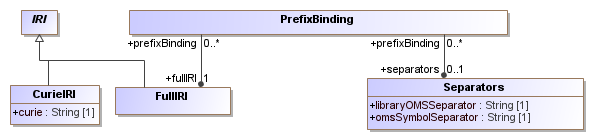
\includegraphics[scale=0.47]{mof/prefixes.png}
  \caption{DOL metamodel: Prefixes}
  \label{fig:prefixes}
\end{figure}

%%%%%%%%%%%%%%%%%%%%%%%%%%%%%%%%%%%%%%%%%%%%%%%%%%%%%%%%%%%%%%%%%%%%%%%%%%%%%%%%%%%%%%%%%%%%%%%%%%%%%%%%%%%%%%%%%%%%%%%%%%%%%%%%%%
%%%%%%%%%%%%%%%%%%%%%%%%%%%%%%%%%%%%%%%%%%%%%%%%%%%%%%%%%%%%%%%%%%%%%%%%%%%%%%%%%%%%%%%%%%%%%%%%%%%%%%%%%%%%%%%%%%%%%%%%%%%%%%%%%%

\ssclause{Abbreviating IRIs using CURIEs}\label{c:curies}

As IRIs tend to be long, and as syntactic mechanisms for abbreviating them have been standardized, 
it is \recommended that applications employ such mechanisms and support expanding abbreviatory
notations into full IRIs.  For specifying the \emph{semantics} of \DOL, this \IS assumes full IRIs 
everywhere, but the \DOL abstract \emph{syntax} adopts CURIEs (compact URI expressions) as an 
abbreviation mechanism, as it is the most flexible one that has been standardized to date.  

The CURIE abbreviation mechanism works by binding prefixes to IRIs.  A CURIE consists of a 
\emph{prefix}, which may be empty, and a \emph{reference}.  If there is an in-scope binding for the 
prefix, the CURIE is valid and expands into a full IRI, which is created by concatenating the IRI 
bound to the prefix and the reference.  In the following example that uses \DOL prefix map mechanism, one the prefix \url{lang} is bound to \url{http://purl.net/DOL/languages/}, which
means that the CURIE \url{lang:OWL2} will be expanded to the IRI
\url{http://purl.net/DOL/languages/OWL2}. 

\begin{lstlisting}[basicstyle=\ttfamily,language=dolText,escapechar=@,mathescape]
%prefix( :      <http://www.example.org/mereology#>
         owl:   <http://www.w3.org/2002/07/owl#>
         lang:  <http://purl.net/DOL/languages/>
                %% definitions of conforming languages ...
         ser:   <http://purl.net/DOL/serializations/>
                %% ... and their serializations
         log:   <http://purl.net/DOL/logics/>
                %% descriptions of logics ...
         trans: <http://purl.net/DOL/translations/> )%
                %% ... and translations

library Mereology

%% OWL Manchester syntax declaration: 
language lang:OWL2 logic log:SROIQ serialization ser:OWL2/Manchester
[...]
\end{lstlisting}


\DOL adopts the CURIE specification of RDFa Core 1.1 \nref{RDFa}, Section 6 with the following changes:
\begin{itemize}
\item \DOL does not support the declaration of a ``default prefix'' mapping %\CLnote[type=q-aut]{Are such explanatory notes OK here? --- Yes}
(covering CURIEs such as \syntax{:name}).
\item \DOL does support the declaration  of a ``no prefix'' mapping (covering CURIEs such as 
\syntax{name}). If there is no explicit declaration for the ``no prefix'', it defaults to a 
context-sensitive expansion mechanism, which always prepends the \DOL library IRI (in the context of a 
structured OMS where named OMS are referenced) respectively the current OMS IRI (in the context of a basic
OMS) to a symbol name. Both the separator between the \DOL library and the OMS name and that between the 
OMS name and the symbol name can be declared (using the keyword \syntax{separators}), and both default to ``//''.

\item \DOL does not make use of the \syntax{safe\_curie} production.
\item \DOL does not allow binding a relative IRI to a prefix.
\item Concrete syntaxes of \DOL are encouraged but \notrequired to support CURIEs.
\end{itemize}

{CURIES are not required as 
a concession to having an RDF-based concrete syntax among the normative concrete syntaxes.  RDFa is 
the only standardized RDF serialization to support CURIEs so far.  Other serializations, such as 
RDF/XML or Turtle, support a subset of the CURIE syntax, whereas some machine-oriented 
serializations, including N-Triples, only support full IRIs.}

CURIEs can occur in any place where IRIs are allowed, as stated in \cref{c:iris}.

The CURIE grammar of \DOL is summarized in \cref{c:curie-syntax}.

%\ednote{This is concrete syntax. Shouldn't it be moved to chapter \ref{{a:text-syntax}}? --- I have copied it there, altough this is code
%duplication.}

Note that outside the context of a basic OMS the prefix/reference separator of a CURIE is always the colon (\syntax{:}); only for serializations of OMS languages other than \DOL it may be redefined as stated in \cref{c:conform:serialization}.

Prefix mappings can be defined at the beginning of a \DOL library (specified in \cref{c:libraries}; 
these apply to all parts of the \DOL library, including basic OMS as clarified in \cref{c:map-ids}).  
%Their syntax is:

Bindings in a prefix map are evaluated from left to right.  Authors \shouldnot bind the same prefix twice, but if they do, the later binding takes precedence.

\ssclause{Mapping identifiers in basic OMS to IRIs}\label{c:map-ids}

While \DOL uses IRIs as identifiers throughout, OMS languages do not necessarily do; for example:
\begin{itemize}
\item OWL \nref{OWL2}, Section 5.5 does use IRIs.
\item Common Logic \nref{CL} supports them but does not enforce their use.
\item F-logic \cite{flogic} does not use them at all.
\end{itemize}
However, \DOL OMS mappings as well as 
%\CLnote[type=todo]{maybe clarify which ones, by checking the grammar for all occurrences of Symbol}
certain operations on OMS require making unambiguous references to non-logical symbols of basic OMS (\syntax{Symbol}).  Therefore, \DOL provides a function that maps global identifiers used within basic OMS to IRIs.  This mapping affects all non-logical symbol identifiers (such as class names in an OWL ontology), but not locally-scoped identifiers such as bound variables in Common Logic ontologies.  \DOL reuses the CURIE mechanism for abbreviating IRIs for this purpose (\cf \cref{c:curies}).

The IRI of a non-logical symbol identifier in a basic OMS $O$ is determined by the following function:
\begin{algorithmic}
  \REQUIRE $D$ is a \DOL library
  \REQUIRE $O$ is a basic OMS in serialization $S$
  \REQUIRE $\mathit{id}$ is the identifier in question, identifying a symbol in $O$ according to the specification of $S$
  \ENSURE $i$ is an IRI
  \IF{$\mathit{id}$ represents a full IRI according to the specification of $S$}
    \STATE $i\leftarrow\mathit{id}$
  \ELSE
    \STATE \COMMENT{first construct a pattern $\mathit{cp}$ for CURIEs in $S$, then match $\mathit{id}$ against that pattern}
    \IF{the declaration of \DOL-conformance of $S$ redefines the prefix/reference separator character $\mathit{cs}$ (cf.\ \cref{c:conform:serialization})}
      \STATE $\mathit{sep}\leftarrow \mathit{cs}$
    \ELSIF{$S$ forbids prefixed CURIEs}
      \STATE $\mathit{sep}\leftarrow\text{undefined}$
    \ELSE
      \STATE $\mathit{sep}\leftarrow\mathit{:}$ \COMMENT{the standard CURIE separator character}
    \ENDIF
    \STATE \COMMENT{The following statements construct a modified EBNF grammar of CURIEs; see \nref{EBNF} for EBNF, and \cref{c:curies} for the original grammar of CURIEs.}
    \IF{$\mathit{sep}$ is defined}
      \STATE $\mathit{cp}\leftarrow [ \mathit{NCName}, \mathit{sep} ] , \mathit{Reference}$
    \ELSE
      \STATE $\mathit{cp}\leftarrow \mathit{Reference}$
    \ENDIF 
    \IF{$\mathit{id}$ matches the pattern $\mathit{cp}$, where $\mathit{ref}$ matches $\mathit{Reference}$}
      \IF{the match succeeded with a non-empty $\mathit{NCName}$ $\mathit{pn}$}
        \STATE $p\leftarrow\mathit{concat}(pn, \mathit{:})$
      \ELSE
        \STATE $p\leftarrow\text{no prefix}$
      \ENDIF
      \IF{$O$ binds $p$ to an IRI $\mathit{pi}$ according to the specification of $S$}
        \STATE $\mathit{nsi}\leftarrow\mathit{pi}$
      \ELSE
        \STATE $P \leftarrow$ the innermost prefix map in $D$, starting from the place of $O$ inside $D$, and going up the abstract syntax tree towards the root of $D$
        \WHILE{$P$ is defined}
          \IF{$P$ binds $p$ to an IRI $\mathit{pi}$}
            \STATE $\mathit{nsi}\leftarrow\mathit{pi}$
            \STATE \textbf{break} out of the \textbf{while} loop 
          \ENDIF
          \STATE $P \leftarrow$ the next prefix map in $D$, starting from the place of the current $P$ inside $D$, and going up the abstract syntax tree towards the root of $D$
        \ENDWHILE
        \RETURN an error
      \ENDIF
      \STATE $i\leftarrow\mathit{concat}(\mathit{nsi}, \mathit{ref})$
    \ELSE
      \RETURN an error
    \ENDIF
  \ENDIF
  \RETURN $i$
\end{algorithmic}

This mechanism applies to basic OMS given inline in a \DOL library (\syntax{BasicOMS}), not to OMS in external documents (\syntax{NativeDocument}); the latter \shall be self-contained.

While CURIEs used for identifying parts of a \DOL library (\cf \cref{c:curies}) are merely syntactic 
sugar, the prefix map for a basic OMS is essential to determining the semantics of the basic OMS 
within the \DOL library. 


%%%%%%%%%%%%%%%%%%%%%%%%%%%%%%%%%%%%%%%%%%%%%%%%%%%%%%%%%%%%%%%%%%%%%%%%%%%%%%%%%%%%%%%%%%%%%%%%%%%%%%%%%%%%%%%%%%%%%%%%%%%%%%%%%%
%%%%%%%%%%%%%%%%%%%%%%%%%%%%%%%%%%%%%%%%%%%%%%%%%%%%%%%%%%%%%%%%%%%%%%%%%%%%%%%%%%%%%%%%%%%%%%%%%%%%%%%%%%%%%%%%%%%%%%%%%%%%%%%%%%

\ssclause{Concrete Syntax}\label{c:curie-syntax}

\vspace{-1.4em}
\begin{lstlisting}[language=ebnf,escapeinside={@@}]

IRI           ::= '<' FullIRI '>' | CURIE
FullIRI       ::= @$<$ an IRI as defined in \nref{IRI} $>$@
CURIE         ::= MaybeEmptyCURIE -
MaybeEmptyCURIE ::= [Prefix] RefWithoutComma
RefWithoutComma ::= Reference - StringWithComma
StringWithComma ::= UChar* ',' UChar*
UChar         ::= @$<$ any Unicode \nref{UCS} character $>$@ 
Prefix        ::= NCName ':'@$<$ \rm see ``NCName'' in \nref{XMLns}, Section 3 $>$@
Reference     ::= Path [Query] [Fragment]
Path          ::= ipath-absolute | ipath-rootless | ipath-empty @$<$\rm{} as defined in \nref{IRI} $>$@
Query         ::= '?' iquery @$<$\rm{} as defined in \nref{IRI} $>$@
Fragment      ::= '#' ifragment @$<$\rm{} as defined in \nref{IRI} $>$@
\end{lstlisting}


In a CURIE without a prefix, the \syntax{reference} part is \notallowed to match any of the keywords of the \DOL syntax (cf.\ clause \ref{c:keywords}).

\medspace
%%%%%%%%%%%%%%%%%%%%%%%%%%
%%%%%%%%%%%%%%%%%%%%%%%%%%





%% ~\todonote[author=Christoph Lange,date=D:201111081514+01'00',type=todo]{somewhere we need to mention semantic annotations to embedded fragments in conforming OMS languages, \eg \%implied}



%% \sclause{Annotations}\label{s:annotations}

%% \todonote{this subclause will be moved to annex M}
%% ~\todonote[author=Christoph Lange,date=D:201108061340+02'00',type=todo]{Properly integrate this text from our LaRC 2011 paper} Annotations always have a subject, which is identified by an IRI. Where the given OMS language does not provide a way of assigning IRIs to a desired subject of an annotation (\eg if one wants to annotate an import in OWL), a library may employ RDF annotations that use XPointer or \nisref{IETF/RFC 5147} as a means of non-destructively referencing pieces of XML or text by URI.\footnote{We intend to utilize the extensibility of the XPointer framework by developing additional XPointer schemes, \eg for pointing to subterms of Common Logic sentences.}
%
%
% \clause{\DOL Text Serialization}\label{a:text-syntax}
%
% \sclause{Document Type}
%
% \begin{description}
% \item[MIME type] \mimetype{application/dol+text}
% \item[Filename extension] .dol
% \end{description}
%
% \sclause{Concrete Syntax}\label{a:dol-text:concrete}
%
% At several places, the concrete syntax uses the non-terminal
% \syntax{'end'} to mark the end of a definition or declaration. Tools
% may make this \syntax{'end'} optional. However, in this standard,
% the \syntax{'end'} is not marked as optional, because it may be needed to effectively
% disambiguate heterogeneous texts.
%
%
% \ssclause{Documents}
%
% \begin{lstlisting}[language=ebnf,escapeinside={()},morecomment={[l]{\%\%\ }}]
% Document                 = [ PrefixMap ] , DOLLibrary
%                          | NativeDocument ;
% DOLLibrary             = 'library' , LibraryName , Qualification , { LibraryItem } ;
% NativeDocument = ($<$) language and serialization specific ($>$) ;
% LibraryItem             = LibraryImport | OMSDefinition | NetworkDefinition | MappingDefinition
%                           | Qualification ;
% LibraryImport                = 'import' , LibraryName ;
% Qualification            = LanguageQualification | LogicQualification | SyntaxQualification ;
% LanguageQualification             = 'language' , LanguageRef ;
% LogicQualification                = 'logic' , LogicRef ;
% SyntaxQualification               = 'serialization' , SyntaxRef ;
% LibraryName             = IRI ;
% \end{lstlisting}
%
% \begin{lstlisting}[language=ebnf,escapechar=+,morecomment={[l]{\%\%\ }}]
% PrefixMap                = '%prefix(' , { PrefixBinding } , ')%' ;
% PrefixBinding            = BoundPrefix , IRIBoundToPrefix , [ Separators ] ;
% BoundPrefix              = ':' | Prefix ; +$<$\rm see definition in \cref{c:curies}$>$\CLnote[type=q-aut]{I think that, in contrast to OWL Manchester, we can allow prefix names that match keywords of the \DOL syntax, as we are enclosing the whole prefix map into an annotation construct -- right?}+
% IRIBoundToPrefix         = '<' , FullIRI , '>' ;
% Separators               = 'separators' , SeparatorString , SeparatorString ;
% SeparatorString  = SeparatorChar , { SeparatorChar } ;
% SeparatorChar    = ipchar | gen-delims , - , '#' ;
%                    ($<$ \rm as defined in \nref{IRI} $>$)
%
% \end{lstlisting}
%
%  Note that the empty prefix (called ``no prefix'' in \nref{RDFa}, Section 6) is denoted by a colon inside the prefix map, but it is omitted in CURIEs.  This is the style of the OWL Manchester syntax \cite{W3C:NOTE-owl2-manchester-syntax-20091027} but differs from the RDFa Core 1.1 syntax.
%
% \vspace{1em}
%
% \ssclause{Networks}
%
% \begin{lstlisting}[language=ebnf,escapeinside={()},morecomment={[l]{\%\%\ }}]
%
% NetworkDefinition            = 'network' , NetworkName , '=' ,
%                          [ ConservativityStrength ] , Network ;
% NetworkName            = IRI ;
% Network                = NetworkElements , [ ExcludeExtensions ] ;
% NetworkElements        = NetworkElement , { ',' , NetworkElement } ;
% NetworkElement         = [ Id , ':' ] , OMSOrMappingorNetworkRef ;
% ExcludeExtensions      = 'excluding' , ExcludedElement , { ',' , ExcludedElement } ;
% ExcludedElement             = IRI , '->' , IRI
%                          | OMSOrMappingorNetworkRef;
% OMSOrMappingorNetworkRef        = IRI ;
% Id                     = Letter , { LetterOrDigit } ;
% \end{lstlisting}
%
% \ssclause{OMS}\label{a:dol-text:OMS}
%
% While in most cases the translation from concrete to abstract syntax
% is obvious (the structure is largely the same),  both
% \syntax{\%consistent} and \syntax{\%mcons} are translated to
% \syntax{model-conservative}, while both \syntax{\%inconsistent} and
% \syntax{\%notmcons} are translated to
% \syntax{not-model-conservative}. Moreover, both \syntax{closed-world}
% and \syntax{minimize} are translated to \syntax{minimize}.
%
%
% \begin{lstlisting}[language=ebnf,escapeinside={()},mathescape]
% BasicOMS = ($<$)language and serialization specific($>$) ;
% ClosableOMS      = BasicOMS
%                      | OMSRef , [ ImportName ] ;
%
% ExtendingOMS        = ClosableOMS
%                      | MinimizeKeyword , '{' , ClosableOMS , '}' ;
%
% OMS                 = ExtendingOMS
%                      | OMS , Minimization
%                      | OMS , OMSTranslation
%                      | OMS , Reduction
%                      | OMS , Approximation
%                      | OMS , Filtering
%                      | OMS , 'and' , [ ConservativityStrength ] , OMS
%                      | OMS , 'then' , ExtensionOMS
%                      | { Qualification } , ':' , GroupOMS
%                      | 'combine' , NetworkElements , [ ExcludeExtensions ]
%                      | GroupOMS ;
%
% Minimization         = MinimizeKeyword , CircMin , [ CircVars ] ;
% MinimizeKeyword      = 'minimize' | 'closed-world' | 'maximize' | 'free' | 'cofree' ;
% CircMin = Symbol , {  Symbol } ;
% CircVars  = 'vars' ,  ( Symbol , { Symbol } ) ;
%
% GroupOMS            = '{' , OMS , '}'
%                      | OMSRef ;
%
% OMSTranslation          = 'with' , { LanguageTranslation } , SymbolMap
%                      | 'with' , LanguageTranslation , { LanguageTranslation } ;
% LanguageTranslation     = 'translation' , OMSLanguageTranslation ;
%
% Reduction            = 'hide' , { LogicReduction } , SymbolList
%                      | 'hide' , LogicReduction , { LogicReduction }
%                      | 'reveal' ,  SymbolList ;
% LogicReduction       = 'along' , OMSLanguageTranslation ;
%
% SymbolList          = Symbol , { ',' , Symbol } ;
% SymbolMap       = GeneralSymbolMapItem , { ',' , GeneralSymbolMapItem } ;
%
% Extraction           = 'extract' , InterfaceSignature
%                      | 'remove' , InterfaceSignature ;
%
% Approximation        = 'forget' , InterfaceSignature , [ 'keep' , LogicRef ]
%                      | 'keep' , InterfaceSignature , [ 'keep' , LogicRef ]
%                      | 'keep' , LogicRef ;
%
% Filtering            = 'select' , BasicOMS
%                      | 'reject' , BasicOMS ;
%
% ExtensionOMS         = [ ExtConservativityStrength ] , [ ExtensionName ] , ExtendingOMS ;
%
% ConservativityStrength         = Conservative
%                      | '%mono'
%                      | '%wdef'
%                      | '%def' ;
% ExtConservativityStrength      = ConservativityStrength | '%implied' ;
% Conservative         = '%ccons'
%                      | '%mcons'
%                      | '%notccons'
%                      | '%notmcons'
%                      | '%consistent'
%                      | '%inconsistent' ;
%
% InterfaceSignature   = SymbolList ;
%
% ImportName           = '%(' , IRI , ')%' ;
% ExtensionName        = '%(' , IRI , ')%' ;
%
% OMSkeyword          = 'ontology' | 'onto' | 'specification' | 'spec' | 'model' | 'oms' ;
%
% OMSDefinition             = OMSkeyword , OMSName , '=' , [ ConservativityStrength ] ,
%                                    OMS , 'end'  ;
%
% Symbol               = IRI ;
% SymbolMapItem            = Symbol , '|->' , Symbol ;
% GeneralSymbolMapItem          = Symbol
%                      | SymbolMapItem ;
% Sentence             = ($<$)an expression specific to an OMS language($>$) ;
%
% OMSName             = IRI ;
%
% OMSRef              = IRI ;
%
% LanguageRef          = IRI ;
% LogicRef             = IRI ;
% SyntaxRef            = IRI ;
%
% LoLaRef              = LanguageRef
%                      | LogicRef ;
% \end{lstlisting}
%
% \begin{lstlisting}[language=ebnf,mathescape]
% OMSLanguageTranslation        = OMSLanguageTranslationRef
%                      | '->' , LoLaRef ;
%
% OMSLanguageTranslationRef     = IRI ;
% \end{lstlisting}
%
% %\ednote{\%safe is more a statement about an import of a module,
% %and hence should be a statement in an OMS network. Recall:
% %ModuleProperties     =  '\%safe' ; }
%
% The above grammar allows for some grouping ambiguity when using operators in
% OMS definitions. These ambiguities are resolved according to the following
% list, listing operators in decreasing order of precedence:
% \begin{itemize}
%   \item \syntax{minimize}, \syntax{maximize}, \syntax{free}, and \syntax{cofree}.
%   \item \syntax{extract}, \syntax{forget}, \syntax{hide}, \syntax{keep},
%     \syntax{reject}, \syntax{remove}, \syntax{reveal}, \syntax{select}, and
%     \syntax{with}.
%   \item \syntax{and}.
%   \item \syntax{then}.
% \end{itemize}
% Multiple occurrences of the same operator are grouped in a left associative
% manner. In all other cases operators on the same precedence level are not
% implicitly grouped and have to be grouped explicitly. Omitting such an explicit
% grouping results in a parse error.
%
% \ssclause{OMS Mappings}\label{a:dol-text:mappings}
% \index{alignment}
% \begin{lstlisting}[language=ebnf,mathescape]
% MappingDefinition             = InterpretationDefinition | EntailmentDefinition | EquivalenceDefinition | ConservativeExtensionDefinition | AlignmentDefinition ;
%
% InterpretationDefinition            = InterpretationKeyword , InterpretationName , [ Conservative ] , ':' , InterpretationType ,  'end'
%                      | InterpretationKeyword , InterpretationName , [ Conservative ] , ':' , InterpretationType , '=' ,
%                        { LanguageTranslation } , [ SymbolMap ] ,  'end'
%                      | InterpretationKeyword , InterpretationName , '=' , Refinement ,  'end' ;
%
% InterpretationKeyword         = 'interpretation' | 'view' | 'refinement' ;
% InterpretationName            = IRI ;
% InterpretationType            = GroupOMS , 'to' , GroupOMS ;
%
% Refinement           = GroupOMS
%                      | NetworkName
%                      | Refinement , 'then' , Refinement
%                      | GroupOMS , 'refined' , [RefMap] , 'to' , Refinement
%                      | NetworkName , 'refined' , [RefMap] , 'to' , Refinement ;
% RefMap               = 'via' , LanguageTranslation , [ SymbolMap ]
%                      | 'via' , [ LanguageTranslation ] , SymbolMap
%                      | 'via' , NodeMap , { ',' , NodeMap } ;
% NodeMap              = OMSName , '|->' , OMSName , [ 'using' , { LanguageTranslation } , [ SymbolMap ] ] ;
%
% EntailmentDefinition           = 'entailment' , EntailmentName , '=' , EntailmentType , 'end' ;
% EntailmentName       = IRI ;
% EntailmentType       = GroupOMS , 'entails' , GroupOMS
%                      | OMSName , 'in' , Network , 'entails' , GroupOMS
%                      | Network , 'entails' , Network ;
%
% EquivalenceDefinition            = 'equivalence' , EquivalenceName , ':' , EquivalenceType ,  'end' ;
% EquivalenceName            = IRI ;
% EquivalenceType            = GroupOMS , '<->' , GroupOMS  , '=' , OMS
%                      | Network , '<->' , Network , '=' , Network ;
%
% ConservativeExtensionDefinition        = 'module' , ConservativeExtensionName , [ Conservative ] , ':' , ConservativeExtensionType ,
%                        'for' , InterfaceSignature ;
% ConservativeExtensionName           = IRI ;
% ConservativeExtensionType           = GroupOMS , 'of' , GroupOMS ;
%
% AlignmentDefinition  = 'alignment' , AlignmentName ,
%                        [ AlignmentCardinalityPair ] , ':' , AlignmentType ,
%                        [ '=' , Correspondence , { ',' , Correspondence } ] ,
%                        [ 'assuming' , AlignmentSemantics ] ,
%                        'end' ;
%
% AlignmentName            = IRI ;
% AlignmentCardinalityPair           = AlignmentCardinalityForward , AlignmentCardinalityBackward ;
% AlignmentCardinalityForward     = AlignmentCardinality ;
% AlignmentCardinalityBackward    = AlignmentCardinality ;
% AlignmentCardinality            = '1' | '?' | '+' | '*' ;
% AlignmentType            = GroupOMS , 'to' , GroupOMS ;
% AlignmentSemantics            = 'SingleDomain' | 'GlobalDomain'  | 'ContextualizedDomain' ;
%
% Correspondence       = CorrespondenceBlock
%                      | SingleCorrespondence
%                      | '*' ;
% CorrespondenceBlock  = 'relation' , [ Relation ] , [ Confidence ] ,
%                        '{' , Correspondence , { ',' , Correspondence } , '}' ;
% SingleCorrespondence = Symbol , [ Relation ] ,
%                        [ Confidence ] , GeneralizedTerm , [ CorrespondenceId ] ;
% CorrespondenceId     = '%(' , IRI , ')%' ;
% Symbol            = IRI ;
% GeneralizedTerm      = Symbol ;
% Relation          = '>' | '<' | '=' | '%' | 'ni' | 'in' | IRI ;
% Confidence           = Double ;
% \end{lstlisting}
% \begin{lstlisting}[language=ebnf,escapeinside={()}]
% Double               = ($<$ a number $\in [0,1]$ $>$) ;
% \end{lstlisting}
%
%
% \sclause{Identifiers}
%
% \begin{lstlisting}[language=ebnf,escapeinside={()}]
% IRI     = '<' , FullIRI , '>' | CURIE ;
% FullIRI = ($<$ an IRI as defined in \nref{IRI} $>$) ;
% CURIE     = MaybeEmptyCURIE , - ;
% MaybeEmptyCURIE = [ Prefix ] , RefWithoutComma ;
% RefWithoutComma = Reference , - , StringWithComma ;
% StringWithComma = { UChar } , ',' , { UChar } ;
% UChar     = ($<$ any Unicode \nref{UCS} character $>$) ;
% Prefix    = NCName , ':' ; ($<$ \rm see ``NCName'' in \nisref{W3C/TR REC-xml-names:2009}, Section 3 $>$)
% Reference = Path , [ Query ] , [ Fragment ] ;
% Path      = ipath-absolute | ipath-rootless | ipath-empty ;
%             ($<$ \rm as defined in \nref{IRI} $>$)
% Query     = '?' , iquery ; ($<$ \rm as defined in \nref{IRI} $>$)
% Fragment  = '#' , ifragment ; ($<$ \rm as defined in \nref{IRI} $>$)
% \end{lstlisting}
%
% In a CURIE without a prefix, the \syntax{reference} part is \notallowed to match any of the keywords of the \DOL syntax (cf.\ clause \label{c:keywords}).


%%%%%%%%%%%%%%%%%%%%%%%%%%%%%%%%%%%%%%%%%%%%%%%%%%%%%%%%%%%%%%%%%%%%%%%%%%%%%%%%%%%%%%%%%%%%%%%%%%%%%%%%%%%%%%%%%%%%%%%%%%%%%%%%%%
%%%%%%%%%%%%%%%%%%%%%%%%%%%%%%%%%%%%%%%%%%%%%%%%%%%%%%%%%%%%%%%%%%%%%%%%%%%%%%%%%%%%%%%%%%%%%%%%%%%%%%%%%%%%%%%%%%%%%%%%%%%%%%%%%%

\sclause{Lexical Symbols}

The character set for the \DOL text serialization is the UTF-8 encoding of Unicode \nref{UCS}.  However, OMS can always be input in the Basic Latin subset, also known as US-ASCII.\footnote{In this case, IRIs will have to be mapped to URIs following section 3.1 of \nref{IRI}.}  For enhanced readability of OMS, the \DOL text serialization particularly supports the native Unicode glyphs that represent common mathematical symbols (e.g.\ Greek letters)  or operators (e.g.\ $\partial$ for partial derivatives). %\todonote[author=Christoph Lange,type=q-aut]{@Till: I took part of that from the CASL reference manual.  I don't think we want/need to specify more than that.  I wouldn't say anything about ``display formats of lexical symbols'', for example.}


%%%%%%%%%%%%%%%%%%%%%%%%%%%%%%%%%%%%%%%%%%%%%%%%%%%%%%%%%%%%%%%%%%%%%%%%%%%%%%%%%%%%%%%%%%%%%%%%%%%%%%%%%%%%%%%%%%%%%%%%%%%%%%%%%%
%%%%%%%%%%%%%%%%%%%%%%%%%%%%%%%%%%%%%%%%%%%%%%%%%%%%%%%%%%%%%%%%%%%%%%%%%%%%%%%%%%%%%%%%%%%%%%%%%%%%%%%%%%%%%%%%%%%%%%%%%%%%%%%%%%

\ssclause{Keywords and signs}\label{c:keywords}

The lexical symbols of the \DOL text serialization include various keywords and signs that occur as terminal symbols in the context-free grammar in \aref{a:EBNF}.   Keywords and signs that represent mathematical signs are displayed as such, when possible, and those signs that are available in the Unicode character set may also be used for input.

%%%%%%%%%%%%%%%%%%%%%%%%%%%%%%%%%%%%%%%%%%%%%%%%%%%%%%%%%%%%%%%%%%%%%%%%%%%%%%%%%%%%%%%%%%%%%%%%%%%%%%%%%%%%%%%%%%%%%%%%%%%%%%%%%%

\sssclause{Keywords}


Keywords are always written lowercase. The following keywords are reserved, and are not available for use as variables or as CURIEs with no prefix\footnote{In such a case, one can still rename affected variables, or declare a prefix binding for affected CURIEs, or use absolute IRIs instead.  These rewritings do not change the semantics.}, although they can be used as parts of tokens. 
%{\ttfamily %
\begin{multicols}{3}
	

\begin{lstlisting}
alignment 
along 
assuming 
and
closed-world
cofree
combine
cons-ext
end
entails
entailment
equivalence
excluding
extract
free
hide
import
in
for
forget
interpretation
keep
language
library
logic
maximize
model
minimize
network
ni
of
oms
onto
ontology
refined
refinement
reject
relation
remove
result
reveal
select
separators
serialization
spec
specification
substitution
then
to
translation
using 
vars
via
view
where
with
%cons
%ccons
%complete
%consistent
%def
%implied
%inconsistent
%mcons
%mono
%notccons
%notmcons
%prefix
%wdef
\end{lstlisting}
%}
\end{multicols}

%%%%%%%%%%%%%%%%%%%%%%%%%%%%%%%%%%%%%%%%%%%%%%%%%%%%%%%%%%%%%%%%%%%%%%%%%%%%%%%%%%%%%%%%%%%%%%%%%%%%%%%%%%%%%%%%%%%%%%%%%%%%%%%%%%

\sssclause{Key signs}

Table~\ref{tab:key-signs} following key signs are reserved, and are not available for use as complete identifiers.  Key signs that are outside of the Basic Latin subset of Unicode may alternatively be encoded as a sequence of Basic Latin characters.


\newcolumntype{T}{>{\ttfamily}{l}}
\ctable[
  caption={Key Signs},
  label={tab:key-signs},
  pos=h
]{TTT}{
}{\FL
  \rmfamily Sign & \rmfamily Unicode Code Point & \rmfamily Basic Latin substitute \ML
  \{   & U+007B LEFT CURLY BRACKET & \NN
  \}   & U+007D RIGHT CURLY BRACKET & \NN
  :    & U+003A COLON & \NN
  =    & U+003D EQUALS SIGN & \NN
  ,    & U+002C COMMA & \NN
  \rmfamily ↦ & U+21A6 RIGHTWARDS ARROW FROM BAR & |-> \NN
  \rmfamily → & U+2192 RIGHTWARDS ARROW & -> \NN
}

%%%%%%%%%%%%%%%%%%%%%%%%%%%%%%%%%%%%%%%%%%%%%%%%%%%%%%%%%%%%%%%%%%%%%%%%%%%%%%%%%%%%%%%%%%%%%%%%%%%%%%%%%%%%%%%%%%%%%%%%%%%%%%%%%%
%%%%%%%%%%%%%%%%%%%%%%%%%%%%%%%%%%%%%%%%%%%%%%%%%%%%%%%%%%%%%%%%%%%%%%%%%%%%%%%%%%%%%%%%%%%%%%%%%%%%%%%%%%%%%%%%%%%%%%%%%%%%%%%%%%

\sclause{Integration of Serializations of Conforming Languages}
\label{sec:existing-serialization}
Any document providing an OMS in a serialization of a \DOL conforming
language can be used as-is in \DOL, by reference to its IRI.

The following cases apply for injecting identifiers into fragments of OMS languages, depending on the conformance level of the respective serialization of the OMS language used in terms of section~\ref{c:conform:serialization}:
\begin{description}
\item[XML conformance]
  \begin{enumerate}
  \item If the serialization supports annotation of the root element of the fragment of interest, as specified in XML conformance requirement~\ref{it:xml-annotation}, an identifier is assigned by way of an annotation whose predicate is \url{http://www.w3.org/2002/07/owl#sameAs} from the OWL language \nref{OWL2-primer} and whose object is expected to be the desired IRI identifier.
  \item If the \textit{dol:id} XML attribute from the \url{http://www.omg.org/spec/DOL/1.0/xml} namespace is supported on the element, as specified in XML conformance requirement~\ref{it:foreign-xml-namespaces}, its value is expected to be the IRI identifier.
  \item If the \texttt{dol:id} XML element is supported as the first child of the element, as specified in XML conformance requirement~\ref{it:foreign-xml-namespaces}, it is expected to contain exactly one text node whose value is the IRI identifier.
  \end{enumerate}
  It is a \DOL syntax error if \begin{enumerate*}\item an \texttt{owl:sameAs} annotation or a \texttt{dol:id} attribute or child element is present and its value is not, or cannot be interpreted, as a full IRI, or if \item more than one of these three alternative fields (annotation, attribute or child element) is present on an element\end{enumerate*}.
\item[RDF conformance] The RDF data model itself enables the assignment of IRI identifiers to all resources.
\item[Text conformance] Identifiers are added by inserting a special comment immediately\footnote{The serialization \may allow whitespace between the keyword and the comment.} after the structural OMS element to be annotated, or, if this is not allowed and no ambiguity arises from inserting the comment \emph{before} the structural element, by doing the latter.  The complete comment \shall read \texttt{\%(I)\%} if the language uses the \texttt{\%} character to introduce comments, where \texttt{I} is the identifier IRI.  If the language uses a different comment syntax, the \emph{content} of the comment \shall start with \texttt{\%(I)\%}, possibly preceded by whitespace.
\item[Standoff markup conformance] If the given OMS serialization conforms with the \mimetype{text/plain} media type as per standoff markup conformance requirement~\ref{it:standoff-text-plain} but not with XML, \nref{text/plain-URI} shall be used as means of non-destructively assigning a URI to pieces of text in the given OMS serialization.
If the serialization conforms with XML as per requirement~\ref{it:standoff-xpointer}, one of \nref{text/plain-URI} or XPointer (\nref{XPointer}) shall be used. { (As an example, consider the identification of imports in the OWL/XML serialization~\cite{W3C:REC-owl2-xml-serialization-20121211}, which does not provide a native way for assigning identifiers to imports unless modified as suggested in annex~\ref{sec:conformance-owl-xml-rdf}.  For example, in an OMS file \textit{cars.owx}, the import \texttt{<Import>http://example.org/engines</Import>} can be referred to by the IRI \url{cars.owx\#xpointer(/owl:Ontology/owl:Import[text()='http://example.org/engines'])} assuming the right binding for the namespace prefix \textit{owl} in scope.
The same import in the text-based OWL Manchester syntax~\cite{W3C:NOTE-owl2-manchester-syntax-20091027} could be referred to as \url{cars.omn\#line=27} according to \nref{text/plain-URI} if it is on line 27 of the document.)}
\end{description}
\ednote{TODO: injection of identifiers addressed, but we also had \%implied etc.  The latter will probably be handled in a similar way, but I don't know how \emph{exactly}.}

Where the given OMS language does not provide a way of assigning IRIs to a desired subject of an annotation (\eg if one wants to annotate an import in OWL), a document may employ RDF annotations that use XPointer or \nref{text/plain-URI} as means of non-destructively referencing pieces of XML or text by IRI, as specified above. (The extensibility of the XPointer framework may be utilized by developing additional XPointer schemes, \eg for pointing to subterms of sentences in the XCL serialization of Common Logic.) 


%%%%%%%%%%%%%%%%%%%%%%%%%%%%%%%%%%%%%%%%%%%%%%%%%%%%%%%%%%%%%%%%%%%%%%%%%%%%%%%%%%%%%%%%%%%%%%%%%%%%%%%%%%%%%%%%%%%%%%%%%%%%%%%%%%
%%%%%%%%%%%%%%%%%%%%%%%%%%%%%%%%%%%%%%%%%%%%%%%%%%%%%%%%%%%%%%%%%%%%%%%%%%%%%%%%%%%%%%%%%%%%%%%%%%%%%%%%%%%%%%%%%%%%%%%%%%%%%%%%%%
%%%%%%%%%%%%%%%%%%%%%%%%%%%%%%%%%%%%%%%%%%%%%%%%%%%%%%%%%%%%%%%%%%%%%%%%%%%%%%%%%%%%%%%%%%%%%%%%%%%%%%%%%%%%%%%%%%%%%%%%%%%%%%%%%%

\cleardoublepage
\clause{\DOL Semantics}\label{c:semantics}

\sclause{General}
%We pursue a threefold approach of assigning a semantics to the \DOL
%abstract syntax:
%
%\begin{description}
%\item[Direct Model-Theoretic Semantics] On the level of basic
%  OMS, this semantics reuses the existing semantics of the
%  involved logics, as well as translations between these logics.  The
%  semantics of structured \DOL OMS and OMS mappings is specified on
%  top of this.
%\item[Translational Semantics] The semantics of Common Logic is
%  employed for all basic OMS languages, taking advantage of the
%  fact that Common Logic is a common translation target for many
%  OMS languages.  In detail, the translational semantics first
%  translates the \DOL abstract syntax into the abstract syntax of
%  $DOL(\CL)$, where $DOL(\CL)$ is the homogeneous restriction of \DOL
%  to libraries with all parts written in Common Logic
%  only.  The latter is interpreted as in the case of the direct
%  semantics, with basic OMS interpreted in terms of the
%  existing Common Logic semantics.
%\item[Collapsed Semantics] The collapsed semantics extends the
%  translational semantics to a semantics that is fully given specified
%  in Common Logic.  It further translates the abstract syntax
%  $DOL(\CL)$ to Common Logic, and then reuses the semantics of Common
%  Logic, without employing a separate semantics for the \DOL language.
%  Here, the meta and object levels are collapsed into Common Logic,
%  but may still be distinguished by a closer look into the Common
%  Logic theory.
%
%\end{description}

%The model-theoretic nature of the semantics ensures a better representation
%of the model theory than a theory-level semantics would do. In particular,
%Theorem~13 of \cite{ThreeSemantics} ensures that models classes of logical 
%theories represented in Common Logic can be recovered through a model
%translation. This is of particular importance when studying model-theoretic
%properties like finite model or tree model properties.

\DOL is a logical language with a precise formal semantics.  The
semantics gives \DOL a rock-solid foundation, and provides increased
trustworthiness in applications based on OMS written in \DOL.  The
semantics of \DOL is moreover the basis for formal interoperability, as
well as for the meaningful use of logic-based tools for \DOL, such as
theorem provers, model-checkers, satisfiability modulo theories (SMT) solvers etc.  Last but not least,
the semantics has provided valuable feedback on the language design,
and has led to some corrections on the abstract syntax.  These
reasons have lead to inclusion of the semantics in the standard
document proper, even though the semantics is quite technical and
therefore has a more limited readership than the other clauses of
this standard.

The semantics starts with the theoretical foundations. Since \DOL is a
language that can be applied to a variety of logics and logic
translations, it is based on a heterogeneous logical environment.
Hence, the most important need is to capture precisely what a
heterogeneous logical environment is.

The \DOL semantics itself gives a formal meaning to \DOL libraries, OMS
networks, OMS, and OMS mappings. For each syntactic construct
in the abstract syntax,
a \emph{semantic domain} is given. It specifies the range of possible
values for the semantics. Additionally, \emph{semantic rules} are
presented, mapping abstract syntax trees to some suitable semantic
domain.


%%%%%%%%%%%%%%%%%%%%%%%%%%%%%%%%%%%%%%%%%%%%%%%%%%%%%%%%%%%%%%%%%%%%%%%%%%%%%%%%%%%%%%%%%%%%%%%%%%%%%%%%%%%%%%%%%%%%%%%%%%%%%%%%%%
%%%%%%%%%%%%%%%%%%%%%%%%%%%%%%%%%%%%%%%%%%%%%%%%%%%%%%%%%%%%%%%%%%%%%%%%%%%%%%%%%%%%%%%%%%%%%%%%%%%%%%%%%%%%%%%%%%%%%%%%%%%%%%%%%%
\sclause{Theoretical Foundations of the \DOL Semantics}
\label{s:foundations}

 In the following the theoretical foundations of the semantics of \DOL are  specified.
The notions of \emph{institution} and institution 
\emph{comorphism} and \emph{morphism} are introduced, which provide formalizations of the terms 
\termref{logic}, \termref{logic translation} and \termref{logic reduction}, respectively. 

Since \DOL covers OMS written in one or several logical systems, the
\DOL semantics needs to clarify the notion of logical
system. Traditionally, logicians have studied abstract logical systems
as sets of sentences equipped with an entailment relation
$\vdash$. Such an entailment relation can be generated in two ways:
either via a proof system, or as the logical consequence relation for
some model theory.  This specification follows the model-theoretic approach, since
this is needed for many of the \DOL constructs, and moreover, ontology,
modeling and specification languages like OWL, Common Logic, or \CASL
come with a model-theoretic semantics, or (like UML class models)
can be equipped with one.

 An abstract notion of logical system is given by  the notion of
satisfaction system \cite{carnielli2008analysis}, called `rooms' in
the terminology of \cite{CharPar}. They capture the Tarskian notion of
satisfaction of a sentence in a model in an abstract way.
%For the semantics of minimization, we assume a pre-order on models.

\begin{definition}\label{def:room}
A triple $\cR=(\mathit{Sen},{\cM,\models)}$  is called a \defsty{satisfaction system}, or \defsty{room}, if $\cR$ consists of
\begin{itemize}
\item a set $\mathit{Sen}$ of \defsty{sentences},
\item a class
%\footnote{If we want to take model morphisms into account, 
%a \emph{category} of models needs to be given here. However, this is important only
%for the \syntax{\%mono} annotation.}
$\cM$ of \defsty{models}, and
\item a binary relation
${\models} \subseteq \cM \times \mathit{Sen}$, called the \defsty{satisfaction relation}.\quad\qed
\end{itemize}
\end{definition}

\eat{
Two sentences are \emph{semantically
equivalent}, written $\varphi_1\bimodels\varphi_2$, if they are satisfied by
the same models.  Two models are \emph{elementary equivalent}, written
$M_1\equiv M_2$, if they satisfy the same sentences.  A room is
\emph{compact\/} iff $\Delta\models_\Sigma\varphi$ implies
$\Delta'\models_\Sigma\varphi$ for some finite subset $\Delta'$ of $\Delta$.
}

While this signature-free treatment enjoys simplicity and is wide-spread in the literature, many 
concepts and definitions found in logics, e.g.\ the notion of a conservative extension, involve the
\emph{vocabulary} or \emph{signature} $\Sigma$ \label{vocabulary} used in sentences.  Signatures 
can be extended with new non-logical symbols, or some of these symbols can be renamed; abstractly, 
this is captured using signature morphisms. Moreover,  morphisms
between models are also needed in order to give a semantics to \syntax{minimize},
\syntax{maximize}, \syntax{free} and \syntax{cofree}---these constructs
use model morphisms to select certain models, e.g.\ the minimal ones.
This leads to the notion of \emph{institution}. An institution
is nothing more than a family of satisfaction systems, indexed by
signatures, and linked coherently by signature morphisms.


\begin{definition}\label{def:inst}  Let $\Set$ be the
category having all small \textsc{}sets as objects and functions as
arrows, and let $\Cat$ be the category
of categories and functors.\footnote {Strictly speaking, $\Cat$ is not a
category but only a so-called quasicategory, which is a category that
lives in a higher set-theoretic universe.}
An
\defsty{institution} \cite{GoguenBurstall92} is a quadruple $I=(\Sig,\sen,\IMod,{\models})$
consisting of the following:
%
\begin{itemize}
\item a category\footnote{See \cite{AHS}\cite{MacLane} for an introduction into category theory.} $\Sig$ of \emph{signatures} and \emph{signature morphisms},
\item a functor $\sen\map{\Sig}{\Set}$  giving, for each signature $\Sigma$, the set of
\emph{sentences} $\sen(\Sigma)$, and for each signature morphism
$\sigma:{\Sigma}\to{\Sigma'}$, the \emph{sentence translation map}
$\sen(\sigma):{\sen(\Sigma)}\to{\sen(\Sigma')}$, where often
$\sen(\sigma)(\varphi)$ is written as $\sigma(\varphi)$, \item a
functor $\IMod:{\Sig^{op}}\to{\Cat}$ giving, for each signature
$\Sigma$, the category of \emph{realisations}\footnote{To avoid confusion 
with models in the sense of model-driven engineering, we use `realisation` instead of  the commonly used term `model` in logic.} $\IMod(\Sigma)$, and for each
signature morphism $\sigma\map{\Sigma}{\Sigma'}$, the \emph{reduct
functor\/} $\IMod(\sigma):{\IMod(\Sigma')}\to {\IMod(\Sigma)}$, where
often $\IMod(\sigma)(M')$ is written as $M'\forget{\sigma}$, and
$M'\forget{\sigma}$ is called the \emph{$\sigma$-reduct} of $M'$,
while $M'$ is called a \emph{$\sigma$-expansion} of
$M'\forget{\sigma}$,
\item a satisfaction relation
${\models_{\Sigma}}\subseteq|{\IMod(\Sigma)|\times\sen(\Sigma)}$ for
each $\Sigma\in |\Sig|$,
\end{itemize}
%
such that for each $\sigma\map{\Sigma}{\Sigma'}$ in $\Sig$ the following \defsty{satisfaction 
condition} holds:
%
\begin{equation}
\tag{$\star$} \qquad M'\models_{\Sigma'}\sigma(\varphi) \iff
M'\forget{\sigma} \models_{\Sigma} \varphi
\end{equation}
%
for each $M'\in |\IMod(\Sigma')|$ and $\varphi\in \sen(\Sigma)$,
expressing that truth is invariant under change of notation and
context.  \qed
\end{definition}

\begin{definition}[Propositional Logic]\label{Prop}
The signatures of propositional logic are sets $\Sigma$ of propositional symbols, and signature morphisms are just
functions $\sigma:{\Sigma_1}\to{\Sigma_2}$ between these sets. 
A $\Sigma$-realisation is a function $M : {\Sigma}\to{\{True, False\}}$, and the reduct of a 
$\Sigma_2$-realisation $M_2$ along a signature morphism $\sigma:{\Sigma_1}\to{\Sigma_2}$ is 
the $\Sigma_1$-realisation given by the composition of $\sigma$ with $M_2$. $\Sigma$-sentences are built from the
propositional symbols with the usual connectives, and sentence translation is replacing the propositional
symbols in $\Sigma$ along the morphism. Finally, the satisfaction relation is defined by the standard truth-tables
semantics. It is straightforward to see that the satisfaction condition holds.\quad\qed
\end{definition}

\begin{definition}[Common Logic --- \Clogic]\label{sem:CommonLogic}
A common logic signature
$\Sigma$ (called vocabulary in Common Logic terminology) consists of a
set of names, with a subset called the set of discourse names, and a
set of sequence markers.
A $\Sigma$-realisation consists of a set $\UR$,
the universe of reference, with a non-empty subset $\UD\subseteq \UR$,
the universe of discourse, and four mappings:
  \begin{itemize}
   \item $\rel$ from $\UR$ to subsets of $\UD^* = \{\langle x_1,\ldots,x_n \rangle \mid x_1,\ldots,x_n \in \UD\}$ (i.e., the set of finite sequences of
elements of $\UD$);
   \item $\fun$ from $\UR$ to total functions from $\UD^*$ into $\UD$;
   \item $\intCL$ from names in $\Sigma$ to $\UR$, such that
$\intCL(v)$ is in $\UD$ if and only if $v$ is a discourse name;
   \item $\seq$ from sequence markers in $\Sigma$ to $\UD^*$.
  \end{itemize}  A $\Sigma$-sentence is a first-order
sentence, where predications and function applications are written
in a higher-order like syntax: $t(s)$.
Here, $t$ is an arbitrary term, and $s$ is a sequence term, which can
be a sequence of terms $t_1\ldots t_n$, or a sequence marker.
A predication $t(s)$ is interpreted by evaluating the term $t$,
mapping it to a relation using $\rel$, and then asking whether the sequence
given by the interpretation $s$ is in this relation.  
Similarly, a function application $t(s)$ is interpreted using $\fun$.
Otherwise, interpretation of terms and formulae is as in
first-order logic. 
A 
difference to first-order logic is the presence of sequence terms (namely sequence markers and
juxtapositions of terms), which denote sequences in $\UD^*$, with term
juxtaposition interpreted by sequence concatenation.
Note that sequences are essentially a non-first-order feature that
can be expressed in second-order logic.
For details, see \cite{CommonLogic:oldfashioned}.

A \Clogic signature morphism 
consists of two maps between the sets of names and of sequence markers, such that the property of 
being a discourse name is preserved and reflected.\footnote{That  is, a name is a discourse
name if and only if its image under the signature morphism is.}
  Reducts leave $\UR$, $\UD$, 
$\rel$ and $\fun$ untouched, while $\intCL$ and $\seq$ are composed with the appropriate
signature morphism component.\quad\qed
\end{definition}
%

Further examples of institutions are: $\mathcal{SROIQ}(D)$, unsorted first-order logic, 
many-sorted first-order logic, and many others.  Note that the reduct of a realisation 
is generally given by forgetting some of its parts.

For the rest of the section, an arbitrary institution is considered. 

\begin{definition}[Theory]
A \defsty{theory} is a pair $(\Sigma,\Delta)$ where $\Sigma$ is a signature and $\Delta$ is a set of $\Sigma$-sentences.
\end{definition}

Given a theory $T=(\Sigma, \Delta)$, the class of $T$-realisation 
is the class of all
$\Sigma$-realisations $M$ such that $M\models \delta$, 
for each sentence $\delta \in \Delta$.
A theory $(\Sigma, \Delta)$ is \defsty{consistent\/} if at least one 
 $(\Sigma, \Delta)$-realisation exists. 
 \defsty{Semantic entailment} is defined as usual: 
for  a theory $(\Sigma, \Delta)$ and 
$\varphi\in \sen(\Sigma)$, $\Delta$ entails $\varphi$, written $\Delta\models\varphi$, if all realisations satisfying all sentences in
$\Delta$ also satisfy $\varphi$. For a theory $(\Sigma, \Delta)$, we write $\Delta^\bullet$ for the set of all $\Sigma$-sentences $\varphi$ such that $\Delta \models \varphi$. 

\begin{definition}[Theory morphism]
A \defsty{theory morphism} $\phi: (\Sigma, \Delta) \rightarrow (\Sigma',  \Delta')$ is 
   a signature morphism $\phi:\Sigma\rightarrow \Sigma'$ such that $\Delta'\models \phi(\Delta)$.
\end{definition}
\medskip

Institution comorphisms capture the intuition of encoding or embedding a logic into a more expressive one.

\begin{definition}[Institution Comorphism] An \defsty{institution comorphism} from an institution $I = (\Sig^I,$ $ \Mod^I, \Sen^I, \models^I)$ to an institution $J=(\Sig^J, \Mod^J,\Sen^J, \models^J)$ consists of a functor $\Phi : \Sig^I \longrightarrow \Sig^J$, and
two natural transformations $\beta: \Mod^J \circ \Phi^{op} \Longrightarrow \Mod^I$
and $\alpha: \Sen^I \Longrightarrow \Sen^J \circ \Phi$, such that 
for each $I$-signature $\Sigma$, each sentence $\varphi\in\Sen^I(\Sigma)$ and each realisation $M'\in|\Mod^J(\Phi(\Sigma))|$
%
\begin{equation*}
  M'\models^{J}_{\Phi(\Sigma)}\alpha_{\Sigma}(\varphi)
\iff
  \beta_{\Sigma}(M')\models^I_{\Sigma}\varphi.
\end{equation*}
%
holds, called the \defsty{satisfaction condition}.\quad\qed
\end{definition}

\noindent
Here, $\Phi(\Sigma)$ is the translation of the signature $\Sigma$ from
institution $I$ to institution $J$, $\alpha_{\Sigma}(\varphi)$ is the
translation of the $\Sigma$-sentence $\varphi$ to a
$\Phi(\Sigma)$-sentence, and $\beta_{\Sigma}(M')$ is the translation
(or perhaps better: reduction) of the $\Phi(\Sigma)$-realisation $M'$ to a
$\Sigma$-realisation. Naturality of $\alpha$ and $\beta$ means that for each
signature morphism $\sigma:\Sigma_1\rightarrow\Sigma_2$ in $I$ the following 
squares commute:
%
\begin{equation*}
\xymatrix{
\Sen^I(\Sigma_1) \ar[d]_{\Sen^I(\sigma)} \ar[r]^{\alpha_{\Sigma_1}}& \Sen^J(\Phi(\Sigma_1)) \ar[d]^{\Sen^J(\Phi(\sigma))} 
& \Mod^J(\Phi(\Sigma_2)) \ar[r]^{\beta_{\Sigma_2}}  \ar[d]^{\Mod^J(\Phi(\sigma))}&\Mod^I(\Sigma_2) \ar[d]^{\Mod^I(\sigma)}\\ 
\Sen^I(\Sigma_2) \ar[r]_{\alpha_{\Sigma_2}}& \Sen^J(\Phi(\Sigma_2)) 
& \Mod^J(\Phi(\Sigma_1)) \ar[r]_{\beta_{\Sigma_1}} & \Mod^I(\Sigma_1)
}
\end{equation*}

A comorphism is:
\begin{itemize}
  \item \emph{faithful} if logical consequence is preserved and reflected along the
comorphism:
%
\begin{equation*}
  \Gamma\models^I\varphi
\iff
  \alpha(\Gamma)\models^J\alpha(\varphi)
\end{equation*}

 \item \emph{model-expansive} if each $\beta_\Sigma$ is
surjective;

\item \emph{(weakly) exact} 
if
for each signature morphism $\sigma\map{\Sigma_1}{\Sigma_2}$,
the naturality diagram
%
\begin{equation*}
\xymatrix{
 \Mod^J(\Phi(\Sigma_2)) \ar[r]^{\beta_{\Sigma_2}}  \ar[d]^{\Mod^J(\Phi(\sigma))}&\Mod^I(\Sigma_2) \ar[d]^{\Mod^I(\sigma)}\\ 
 \Mod^J(\Phi(\Sigma_1)) \ar[r]_{\beta_{\Sigma_1}} & \Mod^I(\Sigma_1)
}
\end{equation*}
%
admits (weak) amalgamation, i.e.\
any for any two realisations $M_2\in|\Mod^I(\Sigma_2)|$
and $M'_1\in|\Mod^J(\Phi(\Sigma_1))|$
with $M_2\forget{\sigma}=\beta_{\Sigma_1}(M'_1)$,
there is a unique (not necessarily unique) 
$M'_2\in|\Mod^J(\Phi(\Sigma_2))|$
with $\beta_{\Sigma_2}(M'_2)=M_2$
and $M'_2\forget{\Phi(\sigma)}=M'_1$;

 \item a \emph{subinstitution comorphism} if $\Phi$ is
an embedding, each $\alpha_\Sigma$ is injective and each $\beta_\Sigma$
is bijective\footnote{An isomorphism if morphisms of realisations are taken into
account.};

\item an \emph{inclusion comorphism} if 
        $\Phi$ and each $\alpha_\Sigma$ are inclusions, and each
        $\beta_\Sigma$ is the identity.
  
\end{itemize}

It is known that each subinstitution comorphism is model-expansive and 
each model-expansive comorphism
is also faithful.
Faithfulness means that a proof goal $\Gamma\models^I\varphi$
in $I$ can be solved by a theorem prover for $J$ by just feeding the
theorem prover with $\alpha(\Gamma)\models^J\alpha(\varphi)$.
Subinstitution comorphism preserve
the semantics of more advanced \DOL structuring constructs such
as OMS translation and OMS reduction.


\begin{definition}
  Given an institution  $I = (\Sig^I,$ $ \Mod^I, \Sen^I, \models^I)$, the
   institution of its theories, denoted $I^{th}$, can be defined as follows. The category of signatures of $I^{th}$ is the category
   of $I$-theories and $I$-theory morphisms, denoted $\Th^I$.
   For each theory $(\Sigma, \Delta)$, its sentences are just $\Sigma$-sentences in $I$, and
   its realisations are just $\Sigma$-realisations in $I$ that satisfy the sentences in $\Delta$, while the
   $(\Sigma,\Delta)$-satisfaction is the $\Sigma$-satisfaction of sentences in realisations of $I$.
\qed \end{definition}

Using this notion, logic translations can be defined that include axiomatization of parts of the
syntax of the source logic into the target logic.

\begin{definition}

 Let $I = (\Sig^I,$ $ \Mod^I, \Sen^I, \models^I)$ and $J = (\Sig^J, \Mod^J,
\Sen^J, \models^J)$ be two institutions. A \defsty{theoroidal institution comorphism} from $I$ to
$J$ is a institution comorphism from $I$ to $J^{th}$.
\qed\end{definition}

\medskip

Institution morphisms capture the intuition of projecting from a more expressive logic to a less expressive one.

\begin{definition}[Institution Morphism] 
An \defsty{institution morphism} from an institution $I = (\Sig^I,$ $ \Mod^I, \Sen^I, \models^I)$ to
an institution $J = (\Sig^J, \Mod^J,
\Sen^J, \models^J)$ consists of a functor $\Phi : \Sig^I \longrightarrow \Sig^J$, and two
natural transformations $\beta: \Mod^I \Longrightarrow \Mod^J \circ \Phi^{op}$
and $\alpha:  \Sen^J \circ \Phi \Longrightarrow \Sen^I $, such that for each $I$-signature $\Sigma$, each sentence $\varphi\in\Sen^J(\Phi(\Sigma))$ and each realisation $M\in\Mod^I(\Sigma)$
%
\begin{equation*}
  M\models^{I}_{\Sigma}\alpha_{\Sigma}(\varphi)
\iff
  \beta_{\Sigma}(M)\models^J_{\Phi(\Sigma)}\varphi.
\end{equation*}
holds, called the \defsty{satisfaction condition}.\quad\qed
\end{definition}

Colimits are a categorical concept providing means of
combining objects interconnected by morphisms, where the colimit
glues together objects along the morphisms.
They can be employed for constructing larger theories from already available 
smaller ones, see \cite{GoguenBurstall92}. For a formal mathematical definition,
see \ref{sec:colimits}.


A major property of colimits of specifications is \emph{amalgamation} (also related to `exactness' \cite{DGS91}). It can be intuitively explained as 
stating that realisations of given
specifications can be combined to yield a uniquely determined realisation of
a colimit specification, provided that the original realisations coincide on
common components. Amalgamation is a common technical assumption in the 
study of specification semantics
\cite{STbook}.

In the following, fix an arbitrary institution
$I=(\Sig,\Sen,\Mod,\models)$.  

\begin{definition}
Given a network $D\map{J}{\Sig^I}$, 
a family of realisations $\mathcal{M} = \{M_p\}_{j\in |J|}$ is
\emph{consistent with} $D$ (or sometimes compatible with $D$) 
if for each node $p$ of $D$, $M_p \in Mod(D(p))$ and
for each edge $e:p\rightarrow q$, $M_p = M_q\forget{D(e)}$.
  A cocone
$(\Sigma,(\mu_j)_{j\in|J|})$ over the network $D\map{J}{\Sig^I}$ is
called \emph{weakly amalgamable} if it is mapped to a weak limit by $\Mod$.
For realisations, this means that for each $D$-compatible family of
realisations $(M_j)_{j\in|J|}$, there is a $\Sigma$-realisation $M$, called an amalgamation of 
 $(M_j)_{j\in|J|}$,
with
$M\forget{\mu_j}=M_j$ ($j\in|J|$), and similarly for morphisms of
realisations.
 If this realisation is unique, the cocone
is called \emph{amalgamable}. 
$I$ (or $\Mod$) admits \emph{(finite) (weak)
amalgamation} if (finite) colimit cocones are (weakly) amalgamable.
Finally, $I$ is called \emph{(weakly) semi-amalgamable} if 
it has pushouts and admits (weak) amalgamation for these.
\qed\end{definition}

\cite{weakcol} studies conditions for existence of weakly amalgamable cocones
in a heterogeneous setting, where the network consists of signatures (or theories)
in different logics. Since a network may admit more than one weakly amalgamable cocone,
a selection operation is required both for the weakly amalgamable cocone of a network 
and for the (potentially non-unique) amalgamation of a family of realisations compatible with the
network. This allows us to define a function
$colimit$ taking as argument a network of heterogeneous signatures and
returning the selected weakly amalgamable cocone for the network and
a function $\oplus$ taking as argument a family of realisations compatible with a network
and returning its selected amalgamation.

%%%%%%%%%%%%%%%%%%%%%%%%%%%%%%%%%%%%%%%%%%%%%%%%%%%%%%%%%%%%%%%%%%%%%%%%%%%%%%%%%%%%%%%%%%%%%%%%%%%%%%%%%%%%%%%%%%%%%%%%%%%%%%%%%%
%%%%%%%%%%%%%%%%%%%%%%%%%%%%%%%%%%%%%%%%%%%%%%%%%%%%%%%%%%%%%%%%%%%%%%%%%%%%%%%%%%%%%%%%%%%%%%%%%%%%%%%%%%%%%%%%%%%%%%%%%%%%%%%%%%

\sclause{Semantics of \DOL Language Constructs}\label{c:direct-sematics}

The semantics of \DOL is based on a fixed (but in principle arbitrary) heterogeneous logical 
environment.  The semantic domains are based on this heterogeneous logical environment. 
A specific heterogeneous logical environment is given in the annexes.

A heterogeneous logical environment is given by a collection of
OMS languages and OMS language translations\footnote{The
  terms \emph{OMS language} and \emph{serialization} are not
  defined formally. For this semantics, it suffices to know that there
  is a language-specific semantics of basic OMS as defined
  below.}, a collection of institutions, \termref{institution} morphisms and
institution comorphisms (serving as logics, logic reductions and logic
translations), and a collection of serializations. Moreover, some of the institution comorphisms are marked as default translations (but only at most one between a given source and target institution), and there is
a binary relation $\mathit{supports}$ between OMS languages and institutions,
and a binary relation $\mathit{supports}$ between OMS languages and
serializations. 
 Each language is required to have a default logic and serialization. Moreover, we assume
 that institutions, institution morphisms and institution comorphisms
 are uniquely identified by names, and we use
 the notation $\Gamma(n)$ for the institution, institution morphism and institution comorphism identified by the name $n$ int the heterogeneous logical environment $\Gamma$.

We are going to require existence of union and difference operations on the signatures
of an institution in the heterogeneous logical environment.
These concepts could be captured in a categorical setting using \emph{inclusion systems} \cite{DGS91}.
 However, inclusion systems are too strong for the purposes of this specification.  Therefore, weaker assumptions will be used.

\begin{definition}  
 An \emph{inclusive category} \cite{DBLP:conf/birthday/GoguenR04} 
 is a category having a broad subcategory\footnote{That is, with the same objects as the original category.}
which is a partially ordered class with 
a least element (denoted $\emptyset$),
finite products and coproducts, called intersection (denoted $\cap$) and union
(denoted $\cup$) such that for each pair of objects $A, B$, $A \cup B$ is a pushout of $A \cap B$ in the category.
\qed \end{definition}

\noindent
A category \emph{has pushouts which preserve inclusions} iff 
there exists a pushout
%
\begin{equation*}
\xymatrix{
  A  \ar[d] \ar@{^{(}->}[r]& A' \ar[d]\\
  B \ar@{^{(}->}[r] & B'
}
\end{equation*}
%
for each span where one arrow is an inclusion.

A functor between two inclusive categories is inclusive if it takes inclusions in the source category to inclusions in the target category.

\begin{definition}
An institution is \emph{weakly inclusive} if
\begin{itemize}
  \item $\Sig$ is inclusive and has pushouts which preserve inclusions,
  \item $\Sen$ is inclusive, and
  \item each category of realisations has a broad subcategory of inclusions.\quad\qed
\end{itemize}
\end{definition}

Let $I$ be a weakly inclusive institution.  $I$  \emph{has differences}, if there is a binary operation $\setminus$ on signatures, 
such that for each pair of signatures 
$\Sigma_1, \Sigma_2$, the greatest signature $\Sigma$ such that
\begin{enumerate}
  \item $\Sigma \subseteq \Sigma_1$
  \item $\Sigma \cap \Sigma_2 = \emptyset$
\end{enumerate} 
exists and is equal to $\Sigma_1\setminus \Sigma_2$.

We will write $\iota_{A\subseteq B}$ for the inclusion of $A$ in $B$ in an
inclusive category, when such an inclusion exists. If $\cI$ is an inclusive institution
and $\Sigma\subseteq\Sigma'$ is an inclusion of signatures, we write 
$M'\forget{\Sigma}$ for the reduct of a $\Sigma'$-realisation $M'$ along the inclusion
$\iota_{\Sigma\subseteq\Sigma'}$.

To be able to talk about the symbols of a signature in a formal way, it
is required that the category of signatures of an institution is an
inclusive category with symbols, as defined below:

\begin{definition}
An \emph{inclusive category with symbols} is an inclusive category
$\C$ equipped with a faithful functor $|\_|:\C\to\Set$\footnote{That is,
$(\C,|\_|)$ is a concrete category.} that preserves
inclusions.\quad\qed
\end{definition}

Moreover, if $\sigma:\Sigma\to\Sigma'$ is a signature morphism,
it uniquely determines a map $|\sigma|:|\Sigma|\to|\Sigma'|$.

After these preliminaries, we can now list the assumptions made about the
institutions in a heterogeneous logical environment.
It is required that for each institution in the heterogeneous logical environment there is a trivial signature
$\emptyset$ with class of realisations $\cM_\emptyset$ and 
such that there exists a unique signature morphism
from $\emptyset$ to any signature of the institution. Moreover, the existence of a partial union operation on institutions is required, denoted $\bigcup$: 
$L_1 \bigcup L_2 = (L, \rho_1:L_1 \to L, \rho_2 : L_2 \to L)$, when defined, where
$L$ is an institution and $\rho_1$ and
$\rho_2$ are institution comorphisms, giving the embedding of $L_1$ and
respectively $L_2$ in $L$. Finally, some of the comorphisms are marked as default translations and some of the morphisms as default projections, with the condition that between any two institutions at most one comorphism and at most one morphism is marked as default.

For each institution $\cI$
in the heterogeneous logical environment, it is further required that
there is:
%
\begin{itemize}
  \item  a function giving the semantics of a basic OMS. It has the format
$$\mathit{semBasic}_{(lang,logic,ser)}(\Sigma,O) = (\Sigma',\Delta')$$
where $O$ is a \syntax{BasicOMS}, $\Sigma$ gives the context of previous declarations, $\Sigma'$ is the resulting
signature and $\Delta'$ is the resulting set of sentences.
 It is required then that $\Sigma\subseteq\Sigma'$.
  \item a function $makeMorphism_\cI$ that turns symbol maps into signature morphisms,
  \item a function $sameName_\cI$ that takes as arguments two signatures 
  $\Sigma_1$ and $\Sigma_2$ of $\cI$
  and returns as result the list of all pairs of symbols $(s^1_i,s^2_i)$ such that
  $s^1_i\in|\Sigma_1|$ and $s^2_i\in|\Sigma_2|$ and the symbols have the same name.
  The relation represented by $sameName_\cI(\Sigma_1,\Sigma_2)$ must be an
  equivalence relation.
  \item a relativization function $relativize_\cI$ 
  taking as argument a theory and giving as 
  result a theory, and a function
  $theoryOfCorrespondences$ for translating correspondences of alignments
  into sentences in the logic according to a given assumption about the
  semantics of the alignment, both needed in Section \ref{sec:oms-mappings}.
%not needed!  \item a default language and a default language serialization.
\end{itemize}

Further,  for each institution, it is required that there exist union and difference operations on signatures.

\medskip

\DOL follows a model-theoretic approach on semantics: the semantics of OMS will be defined as a class of realisations
over some signature of an institution. This is called \emph{model-level}  semantics. In some cases, but not in all, one can also define
a \emph{theory-level} semantics of an OMS as a set of sentences over some signature of an institution. The two semantics are 
related by the fact that, when both the model-level and the theory-level semantics of an OMS are defined, they are compatible in the 
sense that the class of realisations given by the model-level semantics is exactly the class of realisations of the theory given by the
theory-level semantics. 

 The following unifying notation is used for the two semantics of an OMS $O$:\begin{itemize}
 \item the institution of $O$ is denoted $\Inst(O)$,
  \item the signature of $O$ is denoted $\Sig(O)$ (which is a signature in $\Inst(O)$),
  \item the class of models of $O$ is denoted $\Mod(O)$ (which is a class of realisations over $\Sig(O)$),
  \item the set of axioms of $O$ is denoted $\Th(O)$ (which is a set of sentences over $\Sig(O)$).
\end{itemize}
\noindent Moreover, the semantics of $O$ is the tuple $sem(O) = (I, \Sigma, \cM,\Delta)$
where $\Inst(O) = I$, $\Sig(O) = \Sigma$, $\Mod(O) = \cM$ and $\Th(O) = \Delta$.
In the following, we will freely mix these two equivalent descriptions of the semantics. That is, whenever $sem(O)$ is determined in some the context, then also its components $\Inst(O)$, $\Sig(O)$, $\Mod(O)$ and $\Th(O)$ are determined. Vice versa, if the four components are determined, then so is $sem(O)$.

The theory-level semantics of $O$ can be undefined, and then so is $\Th(O)$. When $\Th(O)$ is defined, $\Mod(O)$ can be obtained as $\Mod(O)=\{M\in\Mod(\Sig(O)) \,|\, M\models\Th(O)\}$.

Intuitively, OMS mappings denote various types of links between two or more OMS. 
The semantics of OMS mappings can be captured uniformly as a graph whose nodes $N$ are labeled with 
\begin{itemize}
 \item $\Name(N)$, the name of the node
 \item $\Inst(N)$, the institution of the node
 \item $\Sig(N)$, the signature of the node
 \item $\Mod(N)$, the class of $\Sig(N)$-realisations of the node
 \item $\Th(N)$, the set of $\Sig(N)$-sentences of the node
\end{itemize}
and 
which has two kinds of edges:
\begin{itemize}
  \item import links (written using single arrows, $S\rightarrow T$)
  \item theorem links (written using double arrows, $S\Rightarrow T$)
\end{itemize}
both labeled with 
heterogeneous signature morphisms between the signatures of the source and target nodes
(i.e.~ 
an edge from the node $S$ to the node $T$ is labeled with a pair 
$(\rho, \sigma)$ where $\rho=(\Phi,\alpha,\beta):\Inst(S)\to\Inst(T)$ is an institution comorphism and
$\sigma:\Phi(\Sig(S))\to\Sig(T)$ is a signature morphism in $\Inst(T)$).
The theory of a node  may be undefined, as in the case of OMS, and when it is defined, 
the class of realisations of that node is the class of models of $\Th(N)$. 
For brevity,  the label of a node may be written as a tuple. Further, it is required that  any OMS can be assigned a unique name. 

The semantics of a network of OMS is a graph
whose nodes are labeled like in the semantics of OMS mappings and 
edges are labeled with heterogeneous signature morphisms. 
The intuition is that
network provide means of putting together graphs of OMS and OMS mappings
and of removing sub-graphs of existing networks. 
% %{(Alternatively,  the edges of the graph of a network could be labeled with
% OMS mappings between the OMS labeling the nodes connected by the edge. This gives a more
% compact representation of the graph of the network, but it has the drawback that
% the subgraph giving the semantics of the mapping is not explicitly available and thus
% one cannot operate on it,~e.g. eliminate just a node of it. Also, creating a combination
% of the network becomes more complicated.)}

The semantics of OMS generally depends on a global environment
$\Gamma$ containing:
 \begin{itemize}
    \item a graph of imports between OMS, as in the semantics of OMS mappings but
          only with import links between nodes, denoted $\Gamma.imports$
    \item a mapping from \syntax{IRI}s to semantics of OMS, OMS mappings, and OMS networks, that 
               is also denoted by $\Gamma$, providing access to previous definitions,
    \item a prefix map, denoted $\Gamma.\prefix$, that stores the declared prefixes,
    \item a triple $\Gamma.\current$ that stores the current language, logic and serialization. 
 \end{itemize}

If $\Gamma$ is such a global environment, $\Gamma[\syntax{IRI} \mapsto \cS]$
extends the domain of $\Gamma$ with \syntax{IRI} and
the newly added value of \syntax{IRI} in $\Gamma$ is the semantic entity $\cS$.
 $\Gamma_\emptyset$ is the empty global environment, i.e.~the domain of $\Gamma_\emptyset$ is the empty set, its import graph $\Gamma.imports$ is empty,
the prefix map is empty and the current triple contains the error logic together with its language and serialization.
The union of two global environments $\Gamma_1$ and $\Gamma_2$, 
denoted $\Gamma_1\cup\Gamma_2$, is defined only if the domains of $\Gamma_1$ and $\Gamma_2$,
and of $\Gamma_1.\prefix$ and $\Gamma_2.\prefix$ are disjoint, and then
$\Gamma_1\cup\Gamma_2(\syntax{IRI}) = \begin{cases}
\Gamma_1(\syntax{IRI})& \mbox{if } \syntax{IRI} \in dom(\Gamma_1) \\
\Gamma_2(\syntax{IRI})& \mbox{if } \syntax{IRI} \in dom(\Gamma_2)
\end{cases}$, 
$\Gamma_1\cup\Gamma_2.imports = \Gamma_1.imports \cup \Gamma_2.imports$,
$\Gamma_1\cup\Gamma_2.\current = \Gamma_1.\current$
and $\Gamma_1\cup\Gamma_2.\prefix = \Gamma_1.\prefix \cup \Gamma_2.\prefix$.
  $\Gamma.\{\prefix = \PMap\}$ represents the global environment that sets the prefix map of 
$\Gamma$ to $\PMap$ and $\Gamma.\{\current  = (lang, logic, ser)\}$ is used for 
updating the current triple of $\Gamma$ to $(lang, logic, ser)$.


%We  assume a \emph{language-specific semantics} of basic
%OMS, inherited from the OMS language.  
%%For a basic OMS in 
%%depending on a triple 
%For a basic OMS $O$ in a language $L$ based on an institution $\I$ we define:
%%$L=(lang,logic,ser)$ comprising of
%%an OMS language, a logic (institution) and a serialization as follows:
%$$sem_L(O) = ()$$
%\semdom{sem_L(\syntax{BasicOMS})=(I, \Sigma,\Delta)}
%%\mbox{
% %   where } \Sigma'\geq\Sigma} 
%%  
%% The signature $\Sigma$ is the \emph{local
%%  environment} of non-logical symbols that have been declared previously to
%%\syntax{BasicOMS}. $\Sigma'\geq\Sigma$ is an extension of $\Sigma$
%%with the non-logical symbols declared in \syntax{BasicOMS}.  $\Delta'$ is a set
%%of sentences over $\Sigma'$. 
%where  $\Sigma$ is a signature in $I$ and $\Delta$ is a set
%of sentences over $\Sigma$. 

%
%We further assume a language-specific semantics of complete (basic,
%but possibly also
%structured) OMS
%$sem(L,\syntax{NativeDocument})=(\Sigma,\cM)$, where
%$\Sigma$ is a signature and $\cM$ a class of models over $\Sigma$.

%Semantics of an OMS declaration/relation is given by a mapping \syntax{IRI}s to semantics of OMS
% $$\Gamma: \syntax{IRI} \rightarrow (OMS \uplus OMS \times OMS \times SigMor)$$\ednote{notation(?)}

 \DOL assumes a \emph{language-specific semantics} of native structured
OMS, inherited from the OMS language. For a native document $D$ 
in a language $L$, logic $L'$ and serialization $S$, 
$semNative_{(L,L',S)}(D)$ denotes the language-specific semantics of $D$.
%Further, \DOL assumes similar language-specific semantics of a basic OMS fragment $O$ in
%the context of previous declarations, which is denoted 
%$sem^{(\cI,\Sigma,\cM,\Delta)}_{(L,L',S)}(O)$.

%%%%%%%%%%%%%%%%%%%%%%%%%%%%%%%%%%%%%%%%%%%%%%%%%%%%%%%%%%%%%%%%%%%%%%%%%%%%%%%%%%%%%%%%%%%%%%%%%%%%%%%%%%%%%%%%%%%%%%%%%%%%%%%%%%
%%%%%%%%%%%%%%%%%%%%%%%%%%%%%%%%%%%%%%%%%%%%%%%%%%%%%%%%%%%%%%%%%%%%%%%%%%%%%%%%%%%%%%%%%%%%%%%%%%%%%%%%%%%%%%%%%%%%%%%%%%%%%%%%%%

\ssclause{Semantics of Documents}
 In this section the semantics of \DOL constructs regarding documents and \DOL libraries is defined. 

\semdom{ 
\begin{array}{ll}
 sem(\syntax{Document})& = \Gamma\\
 & : LogicalEnvironment
\end{array}}

 A document is either a \DOL library, or a native document written
in one of the languages supported by the heterogeneous logical
environment. 


For a \syntax{NativeDocument} $nativeDocument$,
$$sem(nativeDocument) = \Gamma''$$

\noindent where 
$\Gamma' =\Gamma_\emptyset.\{\current = (lang, logic, ser)\} $, with 
$lang, logic, ser$ determined from the extension of the file containing the native document, \\
$postfixLogicIRI(o,l)$ is the string $o?logic=l$,\\
$l_1\ldots, l_n$ are the logics supported by $lang$ for some natural number $n$,\\
$\Gamma_1 = \Gamma'[postfixLogicIRI(IRI, l_1)\mapsto semNative_{(lang,l_1,ser)}(nativeDocument)]$,\\
$\Gamma_2 = \Gamma_1[postfixLogicIRI(IRI, l_2)\mapsto semNative_{(lang,l_2,ser)}(nativeDocument)],\ldots$\\
$\Gamma'' = \Gamma_{n-1}[postfixLogicIRI(IRI, l_n)\mapsto semNative_{(lang,l_n,ser)}(nativeDocument)]$.\\
Note that if the OMS in the native document does not conform with the logic determined by
the extension of the file where the document is stored, 
$sem(nativeDocument)$ will be undefined.

The rule for \syntax{DOLLibrary} is given below.

%%%%%%%%%%%%%%%%%%%%%%%%%%%%%%%%%%%%%%%%%%%%%%%%%%%%%%%%%%%%%%%%%%%%%%%%%%%%%%%%%%%%%%%%%%%%%%%%%%%%%%%%%%%%%%%%%%%%%%%%%%%%%%%%%%

\sssclause{Semantics of libraries}

\semdom{
\begin{array}{ll}
 sem(\syntax{DOLLibrary})& = \Gamma\\
 & : LogicalEnvironment
\end{array}
}

 A \DOL library is list of definitions of OMS, OMS
mappings and OMS networks, starting with an optional prefix map and a qualification.

For a \syntax{DOLLibrary} $dolLibrary$,
$$sem(dolLibrary) = \Gamma'$$
\noindent 
where\\
 $sem(dolLibrary.\syntax{prefixMap}) = PMap$,\\
 $\Gamma_1 = \Gamma_\emptyset.\{\prefix = PMap\}$,\\
  $sem(\Gamma_1, dolLibrary.\syntax{qualification}) = \Gamma_2$,\\
  $sem(\Gamma_2, dolLibrary.\syntax{libraryItem}) = \Gamma'$.

Note  that $dolLibrary$.\syntax{libraryName} is just discarded here.
  However, this name should be the IRI of the document
  containing the \syntax{Document}.  This is known as ``linked data
  compliance''. Tools can issue a warning (not an error), if a
  \syntax{Document} does not follow this practice.

%%%%%%%%%%%%%%%%%%%%%%%%%%%%%%%%%%%%%%%%%%%%%%%%%%%%%%%%%%%%%%%%%%%%%%%%%%%%%%%%%%%%%%%%%%%%%%%%%%%%%%%%%%%%%%%%%%%%%%%%%%%%%%%%%%

\sssclause{Semantics of lists of library items}

\semdom{
\begin{array}{ll}
 sem(\Gamma, Sequence(\syntax{LibraryItem}))& = \Gamma'\\
 & : LogicalEnvironment
\end{array}
} 

If $libItem_1,\ldots,libItem_n$ are all \syntax{LibraryItem}s, 

$$sem(\Gamma, Sequence\{libItem_1, \ldots, libItem_n\}) = \Gamma'$$

\noindent where \\
$sem(\Gamma, libItem_1)= \Gamma_1$,\\
$sem(\Gamma_1, libItem_2)= \Gamma_2$, \ldots\\
$sem(\Gamma_{n-1}, libItem_n)= \Gamma'$.


%%%%%%%%%%%%%%%%%%%%%%%%%%%%%%%%%%%%%%%%%%%%%%%%%%%%%%%%%%%%%%%%%%%%%%%%%%%%%%%%%%%%%%%%%%%%%%%%%%%%%%%%%%%%%%%%%%%%%%%%%%%%%%%%%%

\sssclause{Semantics of library items}

\semdom{
\begin{array}{ll}
 sem(\Gamma, \syntax{LibraryItem})& = \Gamma'\\
 & : LogicalEnvironment
\end{array}
}

For a \syntax{LibraryImport} $\mathit{libImport}$,
$$sem(\Gamma, \mathit{libImport}) = \Gamma \cup \Gamma'$$

\noindent where $sem(\Gamma, libImport.\syntax{libraryName}) = anIRI$ and
$sem(anIRI) = \Gamma'$.

A \syntax{LibraryItem} can also be an \syntax{OMSDefinition}, \syntax{NetworkDefinition} or  \syntax{MappingDefinition}, and equations for these
are given in the next sections. (Annex~\ref{a:queries} also introduces
 \syntax{QueryRelatedDefinition}.)


%%%%%%%%%%%%%%%%%%%%%%%%%%%%%%%%%%%%%%%%%%%%%%%%%%%%%%%%%%%%%%%%%%%%%%%%%%%%%%%%%%%%%%%%%%%%%%%%%%%%%%%%%%%%%%%%%%%%%%%%%%%%%%%%%%

\sssclause{Semantics of a list of qualifications}

\semdom{
\begin{array}{ll}
 sem(\Gamma, Sequence(\syntax{Qualification}))& = \Gamma'\\
 & : LogicalEnvironment
\end{array}
}

If $q_1,\ldots, q_n$ are all \syntax{Qualification}s,
$$sem(\Gamma, Sequence(q_1, \ldots, q_n)) = \Gamma'$$ 
\noindent where
$sem(\Gamma, q_1) = \Gamma_1$, $sem(\Gamma_1,q_2) = \Gamma_2$, $\ldots$,
$sem(\Gamma_{n-1}, q_n) = \Gamma'$.

\sssclause{Semantics of qualifications}

\semdom{
\begin{array}{ll}
 sem(\Gamma,\syntax{Qualification})& = \Gamma'\\
 & : LogicalEnvironment
\end{array}
}

For a \syntax{LanguageQualification} $q$,

$$sem(\Gamma,q)=\Gamma'$$

\noindent where $\Gamma' = \Gamma.\{\current = (q.\syntax{languageRef},logic',ser')\}$ and \\
 $logic'=\twocase{logic(\Gamma.\current)}{q.\syntax{languageRef} \textrm{ supports } logic(\Gamma.\current)}{\textrm{default logic for }q.\syntax{languageRef}}$\\
 $ser'=\twocase{ser(\Gamma.\current)}{q.\syntax{languageRef}\textrm{ supports } ser(\Gamma.\current)}{\textrm{default serialization for }q.\syntax{languageRef}}$

For a \syntax{LogicQualification} $q$,
 $$sem(\Gamma,q)=\Gamma'$$

 \noindent where 
 $\Gamma' = \Gamma.\{\current = (lang',q.\syntax{logicRef},ser')\}$\\
$lang = lang(\Gamma.\current)$, $ser=ser(\Gamma.\current)$\\
$lang'=\twocase{lang}{lang \textrm{ supports }
   q.\syntax{logicRef}} {\textrm{the unique language supporting
   }q.\syntax{logicRef}}
 $\\
$ser' = \twocase{ser}{lang' \textrm{ supports }
   ser} {\textrm{the default serialization for
   }lang'}$ 
 \\
 Note that ``the unique language supporting q.\syntax{logicRef}'' may
 be undefined; in this case, the semantics of $q$
 construct is undefined.

For a \syntax{SyntaxQualification} $q$,
$$sem(\Gamma,q)=\Gamma'$$

\noindent where $lang = lang(\Gamma.\current), logic = logic(\Gamma.\current)$ and\\
$\Gamma'  = \Gamma.\{\current = (lang, logic, q.\syntax{syntaxRef})\}$. 
The semantics is defined only if $\mathit{lang}$ supports q.\syntax{syntaxRef}.


%%%%%%%%%%%%%%%%%%%%%%%%%%%%%%%%%%%%%%%%%%%%%%%%%%%%%%%%%%%%%%%%%%%%%%%%%%%%%%%%%%%%%%%%%%%%%%%%%%%%%%%%%%%%%%%%%%%%%%%%%%%%%%%%%%
%%%%%%%%%%%%%%%%%%%%%%%%%%%%%%%%%%%%%%%%%%%%%%%%%%%%%%%%%%%%%%%%%%%%%%%%%%%%%%%%%%%%%%%%%%%%%%%%%%%%%%%%%%%%%%%%%%%%%%%%%%%%%%%%%%

\ssclause{Semantics of Networks}

The semantics of networks of OMS is given with the help of a directed graph. Its nodes
and edges are specified by the \syntax{NetworkElement}s, which can be OMS, OMS mappings, or OMS networks. Intuitively, the graph of a
network consists of the union of all graphs of the network elements it
contains, where an OMS yields a graph with one isolated node. By convention,
all imports in the graph $\Gamma.imports$ of the current context between nodes that are
specified in the list of \syntax{NetworkElement}s are also included in the graph of 
the network. 
The nodes and edges given in the \syntax{ExcludeExtensions} list are then removed from the graph of the network. 

An additional \syntax{Id} can be specified for each node, with the purpose of letting the user specify a 
prefix in the colimit of a network for the symbols with the origin in that node that must be disambiguated.

 The following auxiliary functions are used: 

\begin{itemize}
\item $insert(G, \Gamma, iri,id)$, where $G$ is a graph, 
      $\Gamma$ is a global environment, $iri$ is an \syntax{IRI} and 
      $id$ is an \syntax{Id}, defined as follows:
 \begin{itemize}
    \item if $iri$ denotes an OMS in $\Gamma$, then
                 a new node named $iri$ and labeled with $\Gamma(iri)$ and with $id$ is added to $G$,
                 unless a node named $iri$ already exists in $G$, and in this case $G$ is left unchanged,
   \item if $iri$ denotes an OMS mapping 
      or a network in $\Gamma$, 
      the result is the union of $G$ with the graph of $\Gamma(iri)$.
 \end{itemize}

\item $removeElement(\Gamma, G, anIRI)$, where $G$ is a graph, 
      $\Gamma$ is a global environment and $anIRI$ is an \syntax{IRI},
      defined as follows: 

 \begin{itemize}
    \item if $anIRI$ denotes an OMS in $\Gamma$, 
          then the node labeled with $anIRI$ and all its incoming and outgoing
                edges are removed from $G$,
   \item  if $anIRI$ denotes an OMS mapping in $\Gamma$, then  
   $\Gamma(anIRI)$ gives a graph $G'$ and two nodes 
   $N_1$ and $N_2$. Then all nodes of $G'$ other than $N_1$ and
   $N_2$ and all the edges of $G'$ are removed from $G$.
   \item if $anIRI$ is a network in $\Gamma$, then all the nodes of its graph and all their incoming and outgoing edges are removed 
               from $G$.
 \end{itemize}
 
 \item $removePaths(\Gamma, G, iri_1, iri_2)$, where $G$ is a graph, 
      $\Gamma$ is a global environment and $iri_1, iri_2$ are \syntax{IRI}s,
 whose result is that
 all paths of imports in $G$ between the nodes labeled with 
 $iri_1$ and $iri_2$ are removed from $G$.

\end{itemize}

Finally, the operation $addImports(\Gamma, G, [iri_1, \ldots, iri_n])$ adds to G
all import edges in $\Gamma.imports$ between nodes which appear 
in the subgraph determined by  $\Gamma(iri_1), \ldots, \Gamma(iri_n)$. 


%%%%%%%%%%%%%%%%%%%%%%%%%%%%%%%%%%%%%%%%%%%%%%%%%%%%%%%%%%%%%%%%%%%%%%%%%%%%%%%%%%%%%%%%%%%%%%%%%%%%%%%%%%%%%%%%%%%%%%%%%%%%%%%%%%

\sssclause{Semantics of network definitions}

\semdom{
\begin{array}{ll}
 sem(\Gamma, \syntax{NetworkDefinition})& = \Gamma'\\
 & : LogicalEnvironment
\end{array}
}

If $n$ is a \syntax{NetworkDefinition},
$$sem(\Gamma, n) = \Gamma'$$
\noindent where $\Gamma' = \Gamma[n.\syntax{networkName} \mapsto sem(\Gamma, n.\syntax{network})]$.

If $n.$\syntax{ConservativityStrength} is \syntax{model-conservative}, the semantics is only
defined if the class of families of realisations compatible with the graph $sem(\Gamma,n.\syntax{network})$ is not empty.

If $n.$\syntax{ConservativityStrength} is \syntax{consequence-conservative}, the semantics is 
 defined only if all signature-free sentences that follow from the network, see entailment of OMS by networks, are tautologies.

If $n.$\syntax{ConservativityStrength} is \syntax{monomorphic}, the semantics is only
defined if the class of families of realisations compatible with the graph 
$sem(\Gamma,n.\syntax{network})$ consist of exactly one isomorphism
class of families of realisations.

If $n.$\syntax{ConservativityStrength} is \syntax{weak-definitional}, the semantics is only
defined if the class of families of realisations compatible with the graph 
$sem(\Gamma,n.\syntax{network})$ is at most a singleton.

If $n.$\syntax{ConservativityStrength} is \syntax{definitional}, the semantics is only
defined if the class of families of realisations compatible with the graph 
$sem(\Gamma,n.\syntax{network})$ is a singleton.

If $n.$\syntax{ConservativityStrength} is \syntax{not-model-conservative}, the semantics is only
defined if the class of families of realisations compatible with the graph $sem(\Gamma,n.\syntax{network})$ is the empty set.

If $n.$\syntax{ConservativityStrength} is \syntax{not-consequence-conservative}, the semantics is 
 defined only if not all signature-free sentences that follow from the network, see entailment of OMS by networks, are tautologies.


%%%%%%%%%%%%%%%%%%%%%%%%%%%%%%%%%%%%%%%%%%%%%%%%%%%%%%%%%%%%%%%%%%%%%%%%%%%%%%%%%%%%%%%%%%%%%%%%%%%%%%%%%%%%%%%%%%%%%%%%%%%%%%%%%%

\sssclause{Semantics of networks}

\semdom{
\begin{array}{ll}
 sem(\Gamma, \syntax{Network})& = G\\
 & : OMSGraph
\end{array}
}

If $n$ is a network, 
$$sem(\Gamma, n)= G'$$
\noindent where $sem(\Gamma, n.\syntax{networkElement}) = G$ and 
$sem(\Gamma, G, n.\syntax{excludedElement}) = G'$.


%%%%%%%%%%%%%%%%%%%%%%%%%%%%%%%%%%%%%%%%%%%%%%%%%%%%%%%%%%%%%%%%%%%%%%%%%%%%%%%%%%%%%%%%%%%%%%%%%%%%%%%%%%%%%%%%%%%%%%%%%%%%%%%%%%

\sssclause{Semantics of sets of network elements}

\semdom{
\begin{array}{ll}
 sem(\Gamma, Set(\syntax{NetworkElement}))& = G\\
 & : OMSGraph
\end{array}
}

If $elem_1, \ldots, elem_n$ are all \syntax{NetworkElement}s,
$$sem(\Gamma, Set\{elem_1, \ldots, elem_n\}) = G$$

\noindent where \\
 $G_1 = sem(\Gamma, G_\emptyset, elem_1)$, where $G_\emptyset$ is the empty graph,\\
 $G_2 = sem(\Gamma, G_1, elem_2)$\\
 $\ldots$\\
 $G_n = sem(\Gamma, G_{n-1}, elem_n)$,\\
 $G = addImports(\Gamma, G_n, [elem_1, \ldots, elem_n])$.


%%%%%%%%%%%%%%%%%%%%%%%%%%%%%%%%%%%%%%%%%%%%%%%%%%%%%%%%%%%%%%%%%%%%%%%%%%%%%%%%%%%%%%%%%%%%%%%%%%%%%%%%%%%%%%%%%%%%%%%%%%%%%%%%%%

\sssclause{Semantics of network elements}

\semdom{
\begin{array}{ll}
 sem(\Gamma, G, \syntax{NetworkElement})& = G'\\
 & : OMSGraph
\end{array}
}

If $networkElement$ is a \syntax{NetworkElement},
$$sem(\Gamma, G, networkElement) = insert(G, \Gamma, networkElement.\syntax{elementRef}.\syntax{iri}, networkElement.\syntax{id})$$


%%%%%%%%%%%%%%%%%%%%%%%%%%%%%%%%%%%%%%%%%%%%%%%%%%%%%%%%%%%%%%%%%%%%%%%%%%%%%%%%%%%%%%%%%%%%%%%%%%%%%%%%%%%%%%%%%%%%%%%%%%%%%%%%%%

\sssclause{Semantics of sets of excluded elements}

\semdom{
\begin{array}{ll}
 sem(\Gamma, G, Set(\syntax{ExcludedElement}))& = G'\\
 & : OMSGraph
\end{array}
}

If $elem_1, \ldots, elem_n$ are all \syntax{ExcludedElement}s,
$$sem(\Gamma, G, Set\{elem_1, \ldots, elem_n\}) = G'$$
\noindent where\\
 $G_1 = sem(\Gamma, G, elem_1)$\\
 $G_2 = sem(\Gamma, G_1, elem_2)$\\
  $\ldots$ \\
 $G' = sem(\Gamma, G_{n-1}, elem_n)$


%%%%%%%%%%%%%%%%%%%%%%%%%%%%%%%%%%%%%%%%%%%%%%%%%%%%%%%%%%%%%%%%%%%%%%%%%%%%%%%%%%%%%%%%%%%%%%%%%%%%%%%%%%%%%%%%%%%%%%%%%%%%%%%%%%

\sssclause{Semantics of excluded elements}

\semdom{
\begin{array}{ll}
 sem(\Gamma, G, \syntax{ExcludedElement})& = G'\\
 & : OMSGraph
\end{array}
}

If $excludedElem$ is a $\syntax{ElementRef}$,
$$sem(\Gamma, G, excludedElem) = removeElement(\Gamma, G, excludedElem.\syntax{iri})$$.

If $excludedElem$ is a $\syntax{PathReference}$,
$$sem(\Gamma, G, excludedElem) = removePaths(\Gamma, G, iri_1, iri_2)$$
\noindent 
where
$iri_1 = excludedElem.\syntax{elementRef}.\syntax{iri}$ 
and $iri_2 = excludedElem.\syntax{elementRef2}.\syntax{iri})$.

\ssclause{Semantics of OMS}

In the rest of this section, given a global environment $\Gamma$ and an
\syntax{OMS} $O$, the notation 
$Env(\Gamma, O)$ is used for the global environment $\Gamma'$ 
such that
$sem(\Gamma, O) = (\Gamma', (\cI,\Sigma,\cM,\Delta))$.


%%%%%%%%%%%%%%%%%%%%%%%%%%%%%%%%%%%%%%%%%%%%%%%%%%%%%%%%%%%%%%%%%%%%%%%%%%%%%%%%%%%%%%%%%%%%%%%%%%%%%%%%%%%%%%%%%%%%%%%%%%%%%%%%%%

\sssclause{Semantics of basic OMS}

\semdom{
\begin{array}{ll}
 sem(\Gamma, \syntax{BasicOMS})& = (\Gamma',(\cI,\Sigma,\cM, \Delta))\\
 & : (LogicalEnvironment, (Institution,Signature,ModelClass, Sentences))
\end{array}
}


For a \syntax{BasicOMS} $O$ 
in a global environment $\Gamma$, the  semantics is defined as follows:  

$$sem(\Gamma, O)= (\Gamma',(\Gamma.logic,\Sigma',\cM', \Delta'))$$ 

\noindent where 
\begin{itemize}
\item  $(\Sigma',\Delta')=\mathit{semBasic}_{(\Gamma.lang,\Gamma.logic, \Gamma.ser)}(O)$, 
\item  $\cM'=\{M\in \Mod(\Sigma') \mid M\models\Delta'\}$ 
\item
$\Gamma'$ is obtained from $\Gamma$ by adding to $\Gamma.imports$ a new
node labeled with the name of $O$, $\Gamma.logic$,$\Sigma'$, $\cM'$ and $\Delta'$.
\end{itemize}


%%%%%%%%%%%%%%%%%%%%%%%%%%%%%%%%%%%%%%%%%%%%%%%%%%%%%%%%%%%%%%%%%%%%%%%%%%%%%%%%%%%%%%%%%%%%%%%%%%%%%%%%%%%%%%%%%%%%%%%%%%%%%%%%%%

\sssclause{Semantics of basic OMS in a local environment}

\semdom{
\begin{array}{ll}
 sem(\Gamma, (\cI, \Sigma, \cM, \Delta), \syntax{BasicOMS})& = (\Gamma',(\cI',\Sigma',\cM', \Delta'))\\
 & : (LogicalEnvironment, (Institution,Signature,ModelClass, Sentences))
\end{array}
}


For a \syntax{BasicOMS} $O$ 
in a global environment $\Gamma$ and local
environment $(\cI, \Sigma, \cM, \Delta)$, its semantics is defined only if
$\Gamma.logic = \cI$
as follows:  

$$sem(\Gamma, (\cI, \Sigma, \cM, \Delta), O)= (\Gamma',(\Gamma.logic,\Sigma',\cM', \Delta'))$$ 

\noindent where 
\begin{itemize}
\item  $(\Sigma',\Delta')=\mathit{semBasic}_{(\Gamma.lang,\Gamma.logic, \Gamma.ser)}(\Sigma,O)$  
\item  $\cM'=\{M\in \cM \mid M\models\Delta'\}$ 
\item
$\Gamma'$ is obtained from $\Gamma$ by adding to $\Gamma.imports$ a new
node labeled with the name of $O$, $\Gamma.logic$,$\Sigma'$, $\cM'$ and $\Delta'$.
\end{itemize}


%%%%%%%%%%%%%%%%%%%%%%%%%%%%%%%%%%%%%%%%%%%%%%%%%%%%%%%%%%%%%%%%%%%%%%%%%%%%%%%%%%%%%%%%%%%%%%%%%%%%%%%%%%%%%%%%%%%%%%%%%%%%%%%%%%

\sssclause{Semantics of closable OMS}

\semdom{
\begin{array}{ll}
 sem(\Gamma, \syntax{ClosableOMS})& = (\Gamma',(\cI,\Sigma,\cM, \Delta))\\
 & : (LogicalEnvironment, (Institution,Signature,ModelClass, Sentences))
\end{array}
}

The semantics of a \syntax{BasicOMS} has been defined above.

The semantics of an \syntax{OMSReference} $O$
is given by $$sem(\Gamma, O) = (\cI, \Sigma, \cM,\Delta)$$
\noindent where $locId = postfixLogicIRI(O.\syntax{omsRef},name(\Gamma.logic))$ 
and
 \begin{itemize}
   \item $postfixLogicIRI(o,l)$ is the string $o?logic=l$
   \item $\cI = \Inst(\Gamma(locId))$,
   \item $\Sigma = \Sig(\Gamma(locId))$
   \item $\cM = \Mod(\Gamma(locId))$
   \item $\Delta = \Th(\Gamma(locId))$
   \item $Env(\Gamma,O)$ extends the graph of imports $\Gamma.imports$
         with a new node for $O$ whose name is either 
         $O.importName$, or, if $O.importName$ is missing, $locId$,
         and whose other components of the label are as defined in the items above,
         and with a new edge from the node labeled with 
         $locId$ to $O$, named $O.\syntax{importName}$ 
         and labeled with the identity on $\Sig(\Gamma(locId))$.  
 \end{itemize}


%%%%%%%%%%%%%%%%%%%%%%%%%%%%%%%%%%%%%%%%%%%%%%%%%%%%%%%%%%%%%%%%%%%%%%%%%%%%%%%%%%%%%%%%%%%%%%%%%%%%%%%%%%%%%%%%%%%%%%%%%%%%%%%%%%

\sssclause{Semantics of closable OMS in a local environment}

\semdom{
\begin{array}{ll}
 sem(\Gamma, (\cI, \Sigma, \cM, \Delta), \syntax{ClosableOMS})& = (\Gamma',(\cI',\Sigma',\cM', \Delta'))\\
 & : (LogicalEnvironment, (Institution,Signature,ModelClass, Sentences))
\end{array}
}

The semantics of a \syntax{BasicOMS} has been defined above.

The semantics of an \syntax{OMSReference} $O$
is defined only if $\Inst(\Gamma(locId)) = \cI$,\\
 where
$locId = postfixLogicIRI(O.\syntax{omsRef},name(\Gamma.logic))$, as follows:
$$sem(\Gamma, (\cI, \Sigma, \cM, \Delta), O)= (\Gamma',(\cI',\Sigma',\cM', \Delta'))$$
\noindent where
 \begin{itemize}
   \item $\cI' = \Inst(\Gamma(locId))$
   \item $\Sigma' = \Sig(\Gamma(locId)) \cup \Sigma$
   \item $\cM' = \{M\in \Mod(\Sigma') \mid M\forget\Sigma \in \cM \text{ and } 
                      M\forget {\Sig(\Gamma(locId))} \in 
                      \Mod(\Gamma(locId))\}$
   \item $\Delta' = \iota_{\Sig(\Gamma(locId)\subseteq \Sigma'}(\Th(\Gamma(locId))) \cup \iota_{\Sigma\subseteq \Sigma'}(\Delta)$
   \item $Env(\Gamma, O)$ extends the graph of imports $\Gamma.imports$
         with a new node for $O$ labeled as defined in the items above
         and with a new edge from the node labeled with 
         $locId$ to $O$, named $O.\syntax{importName}$ 
         and labeled with the inclusion of $\Sigma$ in $\Sigma'$.  
 \end{itemize}


%%%%%%%%%%%%%%%%%%%%%%%%%%%%%%%%%%%%%%%%%%%%%%%%%%%%%%%%%%%%%%%%%%%%%%%%%%%%%%%%%%%%%%%%%%%%%%%%%%%%%%%%%%%%%%%%%%%%%%%%%%%%%%%%%%

\sssclause{Semantics of ExtendingOMS} 
 \semdom{
\begin{array}{ll}
 sem(\Gamma, \syntax{ExtendingOMS})& = (\Gamma',(\cI,\Sigma,\cM, \Delta))\\
 & : (LogicalEnvironment, (Institution,Signature,ModelClass, Sentences))
\end{array} 
}
 
The semantics for \syntax{ClosableOMS} has been defined above.

If $O$ is a  \syntax{RelativeClosureOMS},
$O.\syntax{closureType} = \syntax{minimize}$
and $O' = O.\syntax{closableOMS}$, then 
$$sem(\Gamma, O) = (\Gamma',(\cI,\Sigma,\cM, \Delta))$$
\noindent where
\begin{itemize}
 \item $\cI= \Inst(O')$
 \item $\Sigma = \Sig(O')$
 \item $\cM = 
        \{ M \in  \Mod(O') \mid  M \text{ is minimal in } \Mod(O')\}$ 
        and ``minimal''
is interpreted in the pre-order defined by $M_1\leq M_2$
if there is a homomorphism of realisations $\M_1\to\M_2$.
 \item $\Delta = \bot$ 
 \item $\Gamma'$ is obtained from $\Gamma''=Env(\Gamma, O')$ by adding to $\Gamma''.imports$ a new
node labeled with $(Name(O), \Inst(O),\allowbreak \Sig(O), \allowbreak \Mod(O), \Th(O))$ and
an edge from the node of $O'$ to the node of $O$ labeled with the identity
morphism on $\Sig(O')$.
\end{itemize}
 
The semantics of $O$
is defined similarly for the other three alternatives of $O.\syntax{closureType}$, 
only the class of realisations differs:
\begin{itemize}
\item if $O.\syntax{closureType} = \syntax{maximize}$,
$\cM = 
        \{ M \in  \Mod(O') \mid  M \text{ is maximal in } \Mod(O')\}$
\item if $O.\syntax{closureType} = \syntax{free}$,
$\cM = 
        \{ M \in  \Mod(O') \mid  M \text{ is initial in } \Mod(O')\}$
\item if $O.\syntax{closureType} = \syntax{cofree}$,
$\cM = 
        \{ M \in  \Mod(O') \mid  M \text{ is terminal in } \Mod(O')\}$
\end{itemize}
Here, initial and terminal realisations are defined as in
category theory, see \ref{sec:colimits}. 

%%%%%%%%%%%%%%%%%%%%%%%%%%%%%%%%%%%%%%%%%%%%%%%%%%%%%%%%%%%%%%%%%%%%%%%%%%%%%%%%%%%%%%%%%%%%%%%%%%%%%%%%%%%%%%%%%%%%%%%%%%%%%%%%%%

\sssclause{Semantics of ExtendingOMS in a local environment} 
 
\semdom{
\begin{array}{ll}
 sem(\Gamma, (\cI, \Sigma, \cM, \Delta), \syntax{ExtendingOMS}))& = (\Gamma',(\cI',\Sigma',\cM', \Delta'))\\
 & : (LogicalEnvironment, (Institution,Signature,ModelClass, Sentences))
\end{array}
}

The semantics for \syntax{ClosableOMS} has been defined above.

The semantics for minimization selects the realisations that are minimal
in the class of all realisations with the same interpretation for the
local environment (= fixed non-logical symbols, in the terminology of circumscription).

Formally, if $O$ is a \syntax{RelativeClosureOMS},
$O.\syntax{closureType} = \syntax{minimize}$
and $O'= O.\syntax{closableOMS}$, and\\
$sem(\Gamma, (\cI, \Sigma, \cM, \Delta), O') = 
(\Gamma', (\cI', \Sigma',\cM',\Delta'))$ then
$$sem(\Gamma, (\cI, \Sigma, \cM, \Delta), O)) = (\Gamma'',(\cI'',\Sigma'',\cM'', \Delta''))$$
 \noindent where
\begin{itemize}
 \item $\cI'' = \cI'$
 \item $\Sigma'' = \Sigma'$
 \item $\cM'' = 
        \{ M \in  \cM \mid  M \text{ is minimal in } \{M' \in \cM \mid M'\forget\Sigma = M\forget\Sigma\}\}$ and ``minimal''
is interpreted in the pre-order defined by $M_1\leq M_2$
if there is a homomorphism of realisations $\M_1\to\M_2$
 \item $\Delta'' = \bot$ 
 \item $\Gamma''$ is obtained from $\Gamma'$ by adding to $\Gamma'.imports$ a new
node labeled with $(Name(O), \Inst(O),\allowbreak \Sig(O), \Mod(O), \Th(O))$ and
an edge from the node of $O'$ to the node of $O$ labeled with the identity
morphism on $\Sigma''$.
\end{itemize}

The theory-level semantics for $O$ cannot be defined.



The semantics of $O$
is defined similarly for the other three alternatives of $O.\syntax{closureType}$, 
only the model class differs:
\begin{itemize}
\item if $O.\syntax{closureType} = \syntax{maximize}$,
$\cM'' = 
        \{ M \in  \cM \mid  M \text{ is maximal in } \{M' \in \cM \mid M'\forget\Sigma = M\forget\Sigma\}\}$
\item if $O.\syntax{closureType} = \syntax{free}$,
$\cM'' = 
        \{ M \in  \cM \mid  M \text{ is initial in } \{M' \in \cM \mid M'\forget\Sigma = M\forget\Sigma\}\}$
\item if $O.\syntax{closureType} = \syntax{cofree}$,
$\cM'' = 
        \{ M \in  \cM \mid  M \text{ is terminal in } \{M' \in \cM \mid M'\forget\Sigma = M\forget\Sigma\}\}$
\end{itemize}


%%%%%%%%%%%%%%%%%%%%%%%%%%%%%%%%%%%%%%%%%%%%%%%%%%%%%%%%%%%%%%%%%%%%%%%%%%%%%%%%%%%%%%%%%%%%%%%%%%%%%%%%%%%%%%%%%%%%%%%%%%%%%%%%%%

\sssclause{Semantics of OMS}

\semdom{
\begin{array}{ll}
 sem(\Gamma,\syntax{OMS})& = (\Gamma',(\cI,\Sigma,\cM, \Delta))\\
 & : (LogicalEnvironment, (Institution,Signature,ModelClass, Sentences))
\end{array}
}

The semantics for a \syntax{ClosableOMS} has been defined above.

The semantics for an \syntax{ExtendingOMS} has been defined above.


If $o$ is a \syntax{ClosureOMS},
$$sem(\Gamma, O) = (\Gamma'',(I,\Sigma,\cM',\bot))$$
where 

\begin{align*}
(\Gamma',(I,\Sigma,\cM,\Delta)) &= sem(\Gamma, O.\syntax{oms}),  & \Sigma_{\mathit{closure}} &=sem(\Gamma', \Sigma,O.\syntax{closure}.\syntax{circClosure}), \\
\Sigma_{\mathit{var}} & = sem(\Gamma',\Sigma,O.\syntax{closure}.\syntax{circVars}),
& \Sigma_{\mathit{fixed}} &=\Sigma \setminus (\Sigma_{\mathit{closure}} \cup \Sigma_{\mathit{var}})
\end{align*}
and
\begin{itemize}
\item if $O.\syntax{closure}.\syntax{closureType} = \syntax{minimize}$, then\\
$\cM' = \{ M \in \cM \mid  M\forget{\Sigma_{\mathit{closure}}\cup\Sigma_{\mathit{fixed}}} \text{ is minimal in }    \{M' \in \cM\forget{\Sigma_{\mathit{closure}}\cup\Sigma_{\mathit{fixed}}} \mid M'\forget{\Sigma_{\mathit{fixed}}}=M\forget{\Sigma_{\mathit{fixed}}}\} \}
$
\item if $O.\syntax{closure}.\syntax{closureType} = \syntax{maximize}$, then\\
$\cM' = \{ M \in \cM \mid  M\forget{\Sigma_{\mathit{closure}}\cup\Sigma_{\mathit{fixed}}} \text{ is maximal in }    \{M' \in \cM\forget{\Sigma_{\mathit{closure}}\cup\Sigma_{\mathit{fixed}}} \mid M'\forget{\Sigma_{\mathit{fixed}}}=M\forget{\Sigma_{\mathit{fixed}}}\} \}
$
\item
if $O.\syntax{closure}.\syntax{closureType} = \syntax{free}$, then\\
$\cM' = \{ M \in \cM \mid  M\forget{\Sigma_{\mathit{closure}}\cup\Sigma_{\mathit{fixed}}} \text{ is initial in }    \{M' \in \cM\forget{\Sigma_{\mathit{closure}}\cup\Sigma_{\mathit{fixed}}} \mid M'\forget{\Sigma_{\mathit{fixed}}}=M\forget{\Sigma_{\mathit{fixed}}}\} \}
$
\item
if $O.\syntax{closure}.\syntax{closureType} = \syntax{cofree}$, then\\
$\cM' = \{ M \in \cM \mid  M\forget{\Sigma_{\mathit{closure}}\cup\Sigma_{\mathit{fixed}}} \text{ is terminal in }    \{M' \in \cM\forget{\Sigma_{\mathit{closure}}\cup\Sigma_{\mathit{fixed}}} \mid M'\forget{\Sigma_{\mathit{fixed}}}=M\forget{\Sigma_{\mathit{fixed}}}\} \}
$
\end{itemize}

$\Gamma''$ is obtained from 
       $\Gamma' = Env(\Gamma, O.\syntax{oms})$
       by extending $\Gamma'.imports$
        with a new node for $O$ labeled as in the items above
        and with a new edge from the node of $O.\syntax{oms}$ to the node of $O$
        labeled with the identity morphism on $\Sigma$.

%Translation

The semantics of a \syntax{TranslationOMS} $O$ is given by
$$sem(\Gamma, O) = (\Sigma'',(\cI,\Sigma,\cM,\Delta))$$
\noindent where
\begin{itemize}
 \item $\cI = J$,
 \item $\Sigma = \Sigma'$, when 
 $sem(\Gamma, \Sig(O.\syntax{oms}), O.\syntax{omsTranslation}) = ((\Phi, \alpha, \beta) : \Inst(O.\syntax{oms}) \to J, \sigma:\Phi(\Sig(O.\syntax{oms}))\to \Sigma') $,
 \item $\cM = \{M \in \Mod(\Sigma') \,|\, \beta_{\Sig(O.\syntax{oms})}(M\forget\sigma)\in \Mod(O.\syntax{oms})\}$
 \item $\Delta = \{   Sen^J(\sigma)(\alpha_{\Sig(O.\syntax{oms})}(\delta))  \mid \delta \in \Th(O.\syntax{oms}) \}$. It is defined only if $O.\syntax{oms}$ is flattenable.
 \item $\Gamma''$ is obtained from 
       $\Gamma' = Env(\Gamma, O.\syntax{oms})$
       by extending $\Gamma'.imports$
        with a new node for $O$ labeled as in the items above
        and with a new edge from the node of $O.\syntax{oms}$ to the node of $O$
        labeled with $((\Phi, \alpha, \beta), \sigma)$.
\end{itemize}
%Reduction

The semantics of a \syntax{ReductionOMS} $O$ is
$$sem(\Gamma, O) = (\Gamma'',(\cI,\Sigma,\cM,\Delta))$$
\noindent where
\begin{itemize}
  \item $\cI = J$, 
  \item $\Sigma = \Sigma'$, when
   $sem(\Gamma, \Sig(O.\syntax{oms}), O.\syntax{reduction}) = ((\Phi, \alpha, \beta) : \Inst(O.\syntax{oms}) \to J,\sigma:\Sigma'\to \Phi(\Sig(O.\syntax{oms})))$,
  \item $\cM = \{\beta_\Sigma(M)\forget{\sigma} \mid M\in \Mod(O.\syntax{oms})\}$
  \item $\Delta = \bot$
  \item $\Gamma''$ is obtained from 
       $\Gamma' = Env(\Gamma, O.\syntax{oms})$
       by extending $\Gamma'.imports$
        with a new node for $O$ labeled as in the items above
        and with a new edge from the node of $O$ to the node of 
        $O.\syntax{oms}$ labeled with
        $((\Phi, \alpha, \beta),\sigma)$.
\end{itemize}

%Module Extract 

The semantics of an \syntax{ExtractionOMS} $O$
is
$$sem(\Gamma, O) = (\Gamma'',(\cI,\Sigma,\cM,\Delta))$$
\noindent where
\begin{itemize}
  \item $\cI = \Inst(O.\syntax{oms})$
  \item $\Sigma = \Sigma'$,
  \item $\Delta = \Delta'$
  \item $\cM$ is the class of $\Delta$-realisations
  \item $\Gamma''$ is obtained from 
       $\Gamma' = Env(\Gamma, O.\syntax{oms})$
       by extending $\Gamma'.imports$
        with a new node for $O$ labeled as in the items above
        and with a new edge from the node of $O$ to the node of 
        $O.\syntax{oms}$ labeled with
        the inclusion of $\Sigma'$ in $\Sig(O.\syntax{oms})$
\end{itemize}
where 
$sem(\Gamma, (\Sig(O.\syntax{oms}), \Th(O.\syntax{oms})), O.\syntax{extraction}) = 
(\Sigma',\Delta')$.
%which in turn amounts to stating that each $\Sigma' \cup \Sigma$-reduct
%of a $\Mod(\Sig(O))$-model can be expanded to a $\Mod(\Sig(O))$-model
%satisfying $\Th(O) \setminus \Delta'$.

%Approximation
The semantics of an \syntax{ApproximationOMS} $O$ is
$$sem(\Gamma, O) = (\Gamma'',(\cI'',\Sigma',\cM,\Delta))$$
\noindent where
\begin{itemize}
  \item $\cI'' = \cI'$,
  \item $\Sigma' = \Phi(\Sigma)$
  \item $\Delta = \alpha^{-1}_{\Sig(O.\syntax{oms})}(\Th(O.\syntax{oms})^\bullet)\cap\Sen^{\cI'}(\Sig(O.\syntax{oms}))$.
, i.e.\ that part of $\Th(O.\syntax{oms})$ that can be expressed in the smaller signature and logic . In  practice, one looks for a finite subset that still is logically equivalent to this set.
  \item $\cM$ is the class of $\Delta$-realisations
  \item $\Gamma''$ is obtained from 
       $\Gamma' = Env(\Gamma, O.\syntax{oms})$
       by extending $\Gamma'.imports$
        with a new node for $O$ labeled as in the items above
        and with a new edge from the node of $O.\syntax{oms}$ to the node of $O$ 
        labeled with $(\rho,\iota: \Phi(\Sigma) \to \Sig(O.\syntax{oms}))$ 
\end{itemize}
\noindent where $(\rho = (\Phi,\alpha,\beta):\cI\to\cI',\Sigma) = sem(\Gamma, (\Inst(O.\syntax{oms}), \Sig(O.\syntax{oms})), O.\syntax{approximation})$.

%Filtering
The semantics of a \syntax{FilteringOMS} $O$
is defined by case distinction.
Let
 $(\Gamma',(\cI,\Sigma,\cM, \Delta)) = sem(\Gamma, O.\syntax{oms})$ and
 $(c, \cI',\Sigma',\Delta') = sem(\Gamma', (\cI, \Sigma, \cM, \Delta), O.\syntax{filtering})$.
 
If $c = keep$, 
the semantics of $O$ is given by
$$sem(\Gamma, O) = (\Gamma'',(\cI'',\Sigma'',\cM'',\Delta''))$$
\noindent where
\begin{itemize}
  \item $\cI'' = \cI'$
  \item $\Sigma''$ is the smallest signature
with $\Sigma'\subseteq\Sigma''$ and $\Delta'\subseteq\Sen(\Sigma'')$. ({If this smallest signature does not exist, the semantics is undefined.})
  \item $\Delta'' = (\Delta\cap\Sen(\Sigma''))\cup\Delta'$
  \item $\Mod(O)$ is the class of all $\Delta$-realisations
  \item $\Gamma''$ is obtained from 
       $\Gamma'$
       by extending $\Gamma'.imports$
       with a new node for $O$ labeled as in the items above and
       with a new edge from the node of $O$ to the node of $O.\syntax{oms}$
        labeled with the inclusion of $\Sigma''$ in $\Sigma$.
\end{itemize}

\noindent
If $c = remove$, the semantics of $O$  
is
$$sem(\Gamma, O) = (\Gamma'',(\cI'',\Sigma'',\cM'',\Delta''))$$
\noindent where
\begin{itemize}
  \item $\cI'' = \cI'$
  \item $\Sigma'' = \Sigma\setminus \Sigma'$ 
  \item $\Delta'' = \Delta\cap\Sen(\Sigma'')\setminus\Delta'$
  \item $\cM''$ is the class of all $\Th(O)$-realisations
    \item $\Gamma''$ is obtained from 
       $\Gamma'$
       by extending $\Gamma'.imports$
       with a new node for $O$ labeled as in the items above and
       with a new edge from the node of $O$ to the node of $O.\syntax{oms}$
        labeled with the inclusion of $\Sigma''$ in $\Sigma$.
\end{itemize}

%Union

The semantics of an \syntax{UnionOMS} $O$ is
$$sem(\Gamma, O) = (\Gamma'',(\cI',\Sigma',\cM',\Delta'))$$
\noindent where
\begin{itemize}
  \item $\cI' = \cI$ where
    $\Inst(O_1) \bigcup \Inst(O_2) =(\cI, (\Phi_1, \alpha_1,\beta_1) : \Inst(O_1) \rightarrow \cI, 
                    (\Phi_2, \alpha_2,\beta_2) : \Inst(O_2) \rightarrow \cI)$
  \item $\Sigma' = \Phi_1(\Sig(O_1)) \cup \Phi_2(\Sig(O_2))$
  \item $\cM' = \{ M\in \Mod^\cI(\Sigma') \mid \beta_{\Sigma_i}(M\forget{\Phi_i(\Sig(O_i))}) \in \Mod(O_i), \text{ for } i=1,2 \}$
  \item $\Delta' = \alpha_1(\Th(O_1)) \cup \alpha_2(\Th(O_2))$.
    \item 
        $\Gamma''$ is obtained from 
       $\Gamma' = Env(Env(\Gamma,O_1), O_2)$
       by extending $\Gamma'.imports$
       with a new node for $O$ labeled as in the items above and
       with edges from the nodes of $O_1$ and $O_2$,
       respectively, to the node of $O$,
        labeled for each $i=1,2$ with
        $(\Phi_i, \alpha_i,\beta_i, \iota_i: \Phi_i(O_i) \to \Sigma')$.
\end{itemize}
where $O_1 = O.\syntax{oms}$ and $O_2 = O.\syntax{oms2}$. 

If $O.\syntax{conservativityStrength}$ is present, then $O$ must be a conservative extension
of the appropriate strength of $O_1$.

%Extension

The semantics of an \syntax{ExtensionOMS} $O$ is
$$sem(\Gamma, O) = (\Gamma'',(\cI',\Sigma',\cM',\Delta'))$$
\noindent where
\begin{itemize}
  \item $\cI' = \Inst(O.\syntax{oms}) = \Inst(O.\syntax{extension})$ 
  (which means that
  the institutions of $O.\syntax{oms}$ and 
  $O.\syntax{extension}$ must be the same)
  \item $\Sigma' = \Sig(O.\syntax{oms}) \cup 
  \Sig(sem(\Gamma, 
       (\Inst(O.\syntax{oms}), \Sig(O.\syntax{oms}), \Mod(O.\syntax{oms}), \Th(O.\syntax{oms}) ),
  O.\syntax{extension})$
  \item $\cM' = \{ M\in \Mod(\Sigma') \mid M\forget{\Sig(O.\syntax{oms})} \in \Mod(O.\syntax{oms})
  \text{ and }
  M \forget{\Sig(O.\syntax{extension})} \in \Mod(O.\syntax{extension})\}$
  \item $\Delta' = \Th(O.\syntax{oms}) \cup \Th(O.\syntax{extension})$
  \item $\Gamma''$ is $Env(Env(\Gamma, O.\syntax{oms}), O.\syntax{extension})$.
\end{itemize}

%Qualification
 
The semantics of a \syntax{QualifiedOMS} $O$ 
in the context $\Gamma$ is the same as the
semantics of $O.\syntax{oms}$ in the context
$\Gamma'$ given by the semantics of
$O.\syntax{qualification}$ in the context $\Gamma$.
The change of context is local to $O.\syntax{oms}$, which
means that if the qualification appears as a term in 
a larger expression, after its analysis the context will
be $\Gamma$ and not $\Gamma'$.
Formally,
$$sem(\Gamma, O) = (\Gamma'', (\cI,\Sigma, \cM, \Delta))$$
\noindent where $(\Gamma'',(\cI,\Sigma,\cM,\Delta)) = 
sem(sem(\Gamma, O.\syntax{qualification}), 
    O.\syntax{oms})$.

%Combination

The semantics of a \syntax{CombinationOMS} $O$ is
$$sem(\Gamma, O) = (\Gamma'',(\cI',\Sigma',\cM',\Delta'))$$
\noindent where
\begin{itemize}
  \item $\cI' = \cI$,
  \item $\Sigma' = \Sigma$, where $(\cI,\Sigma,  \{\mu_i\}_{i\in |G|})$ is the colimit of the graph $G = sem(\Gamma,O.\syntax{network})$,
  \item $\Delta' = \cup_{i\in |G|} \mu_i(\Th(O_i))$, where $O_i$ is the OMS label of the node $i$ in $G$
  \item $\cM' =  \{ M\in\Mod(\Sigma) \mid M\forget{\mu_i} \in \Mod(O_i), i\in |G| \}$, where $O_i$ is the OMS label of the node $i$ in $G$.
  \item $\Gamma''$ is obtained from $\Gamma$ by adding to $\Gamma.imports$ 
  a new node for $O$ labeled as in the items above and with edges from each node in
  $G$ to this new node labeled with the morphisms $\mu_i$ for each $i\in |G|$.
\end{itemize}


%%%%%%%%%%%%%%%%%%%%%%%%%%%%%%%%%%%%%%%%%%%%%%%%%%%%%%%%%%%%%%%%%%%%%%%%%%%%%%%%%%%%%%%%%%%%%%%%%%%%%%%%%%%%%%%%%%%%%%%%%%%%%%%%%%

\sssclause{Semantics of \syntax{CircClosure}}
\semdom{
\begin{array}{ll}
 sem(\Gamma,\Sigma, \syntax{CircClosure})& = \Sigma'\\
 & : Signature
\end{array}
}
If $c$ is a \syntax{CircClosure},
$$sem(\Gamma,\Sigma, c) = sem(\Gamma, \Sigma, c.symbol)$$
%%%%%
\sssclause{Semantics of \syntax{CircVar}}
\semdom{
\begin{array}{ll}
 sem(\Gamma,\Sigma, \syntax{CircVar})& = \Sigma'\\
 & : Signature
\end{array}
}
If $c$ is a \syntax{CircVar},
$$sem(\Gamma,\Sigma, c) = sem(\Gamma, \Sigma, c.symbol)$$


%%%%%%%%%%%%%%%%%%%%%%%%%%%%%%%%%%%%%%%%%%%%%%%%%%%%%%%%%%%%%%%%%%%%%%%%%%%%%%%%%%%%%%%%%%%%%%%%%%%%%%%%%%%%%%%%%%%%%%%%%%%%%%%%%%

\sssclause{Semantics of OMS translations}

\semdom{
\begin{array}{ll}
 sem(\Gamma,\Sigma, \syntax{OMSTranslation})& = (\rho,  \sigma)\\
 & : (Comorphism, SignatureMorphism)
\end{array}
}

The semantics of a \syntax{OMSTranslation}
$O=$
is given by
\begin{itemize}
 \item $\rho= sem(O.\syntax{omsLanguageTranslation}) : \Gamma.logic \to logic'$
 \item $\sigma = sem(\Gamma.\{\current=(lang', logic', ser')\}, \Phi(\Sigma), O.\syntax{symbolMap})$
\end{itemize}
\noindent where
$lang'$ and $ser'$ are the default language and serialization for logic $logic'$.
If $O.\syntax{omsLanguageTranslation}$ is missing, 
it defaults to the identity comorphism of the current logic.


%%%%%%%%%%%%%%%%%%%%%%%%%%%%%%%%%%%%%%%%%%%%%%%%%%%%%%%%%%%%%%%%%%%%%%%%%%%%%%%%%%%%%%%%%%%%%%%%%%%%%%%%%%%%%%%%%%%%%%%%%%%%%%%%%%

\sssclause{Semantics of OMS language translations}

\semdom{
\begin{array}{ll}
 sem(\Gamma,\syntax{OMSLanguageTranslation})& = \rho\\
 & : Translation
\end{array}
}

If $t$ is a \syntax{NamedLanguageTranslation},
$$sem(\Gamma,t)=\Gamma(O.\syntax{omsLanguageTranslationRef})$$
\noindent where $\Gamma(O.\syntax{omsLanguageTranslationRef})$ is
an institution comorphism.  This is defined only if the
domain of $\rho$ is the current logic of $\Gamma$.

If $t$ is a \syntax{DefaultTranslation},
$$sem(\Gamma, t)=\rho$$
\noindent where $\rho$ is the
unique default institution comorphism of the heterogeneous logical
environment running from $\Gamma.logic$ to $t.\syntax{languageRef}$ (if this is a
logic) or to some logic supported by $t.\syntax{languageRef}$ (if this
is a language). If there is no or no unique such comorphism, the
semantics is undefined. 

\semdom{
\begin{array}{ll}
 sem(\Gamma,Sequence(\syntax{OMSLanguageTranslation}))& = \rho\\
 & : Translation
\end{array}
}

If $t_1, \ldots, t_n$ are all \syntax{OMSLanguageTranslation}s,
$sem(\Gamma, Sequence\{t_1, \ldots, t_n\}) = \rho$,
where
$sem(\Gamma, t_i) = \rho_i$ for 
$i=1,\ldots, n$ and
 $(\Phi,\alpha,\beta) = \rho_1;\rho_2;\ldots;\rho_n$. 


%%%%%%%%%%%%%%%%%%%%%%%%%%%%%%%%%%%%%%%%%%%%%%%%%%%%%%%%%%%%%%%%%%%%%%%%%%%%%%%%%%%%%%%%%%%%%%%%%%%%%%%%%%%%%%%%%%%%%%%%%%%%%%%%%%

\sssclause{Semantics of reductions}

\semdom{
\begin{array}{ll}
 sem(\Gamma, \Sigma, \syntax{Reduction})& = (\rho, \sigma)\\
 & : (Morphism, SignatureMorphism)
\end{array}
}

The semantics of a \syntax{Reduction}
$O=$ with $O.\syntax{reduction}.\syntax{removalKind} = remove$
is given by
\begin{itemize}
 \item $\rho = sem(O.\syntax{reduction}.\syntax{omsLanguageTranslation}) : \Gamma.logic \to logic'$
 \item 
$\sigma = 
\iota: \Sigma' \to \Phi(\Sigma)$, where 
$\Sigma' = sem(\Gamma.\{\current=(lang', logic', ser')\}, \Phi(\Sigma), O.\syntax{reduction}.\syntax{symbolList})$,
$lang'$ and $ser'$ are the default language and serialization for logic $logic'$
and $\iota$ is the inclusion morphism.
\end{itemize}

If $O.\syntax{reduction}.\syntax{omsLanguageTranslation}$ is missing, 
it defaults to the identity morphism of the current logic of $\Gamma$.


The semantics of a reduction
$O=$  with $O.\syntax{reduction}.\syntax{removalKind} = keep$
is 
 \begin{itemize}
  \item $\rho$ is the identity morphism on the current logic of $\Gamma$
  \item $\sigma$ is the inclusion of
  $sem(\Gamma, \Sigma, O.\syntax{reduction}.\syntax{symbolList})$ in
   $\Sigma$.
 \end{itemize}

%%%%%%%%%%%%%%%%%%%%%%%%
%
%\semdom{sem(\Gamma, L, \syntax{LogicReduction}) = (\Phi, \alpha,\beta)}
%
%$sem(\Gamma, \syntax{IRI})=(\Phi,\alpha,\beta)$,
%where $(\Phi,\alpha,\beta)$ is the institution morphism
%named by \syntax{IRI} in the heterogeneous logical environment.


%%%%%%%%%%%%%%%%%%%%%%%

%%%%%%%%%%%%%%%%%%%%%%%%%%%%%%%%%%%%%%%%%%%%%%%%%%%%%%%%%%%%%%%%%%%%%%%%%%%%%%%%%%%%%%%%%%%%%%%%%%%%%%%%%%%%%%%%%%%%%%%%%%%%%%%%%%

\sssclause{Semantics of sets of symbols}

\semdom{
\begin{array}{ll}
 sem(\Gamma, \Sigma, Set(\syntax{Symbol}))& = \Sigma'\\
 & : Signature
\end{array}
 }

If $s_1,\ldots, s_n$ are all \syntax{Symbol}s,
$$sem(\Gamma, \Sigma, Set\{s_1,\ldots, s_n\}) = \Sigma'$$
where $\Sigma'$ is the smallest sub-signature of $\Sigma$ containing
$sem(\Gamma, \Sigma,s_1), \ldots, 
sem(\Gamma,\Sigma,s_n)$, if such a sub-signature exists and is otherwise undefined.


%%%%%%%%%%%%%%%%%%%%%%%%%%%%%%%%%%%%%%%%%%%%%%%%%%%%%%%%%%%%%%%%%%%%%%%%%%%%%%%%%%%%%%%%%%%%%%%%%%%%%%%%%%%%%%%%%%%%%%%%%%%%%%%%%%

\sssclause{Semantics of symbol maps}

\semdom{
\begin{array}{ll}
sem(\Gamma,\Sigma, \syntax{SymbolMap})& = \sigma:\Sigma\to\Sigma'\\
 & : SignatureMorphism
\end{array}
}

If $r$ is a \syntax{SymbolMap} such that for every 
\syntax{SymbolMapItem} $gItem$ in $r.\syntax{generalSymbolMapItem}$
we have that $gItem.\syntax{source}$ is a symbol in $|\Sigma|$ 
and
for every 
\syntax{Symbol} $s$ in $r.\syntax{generalSymbolMapItem}$
we have that $s$ is a symbol in $|\Sigma|$,
$$sem(\Gamma,\Sigma,r) = \sigma: \Sigma\to\Sigma'$$
\noindent where 
$\sigma$ must be the unique signature morphism with the properties
\begin{enumerate}
\item $\sigma$ matches $r$: for each \syntax{SymbolMapItem} 
$r.\syntax{generalSymbolMapItem}$ $gItem$ in 
$r.\syntax{generalSymbolMapItem}$, we have that
$|\sigma|(gItem.\syntax{source}) = gItem.\syntax{target}$ and for each 
\syntax{Symbol} $s$ in $r.\syntax{generalSymbolMapItem}$,
$|\sigma|(s) = s$,
\item $\sigma$ is the identity outside the domain of $r$:
for each symbol $s\in|Sigma|$ such that there is no \syntax{SymbolMapItem}
$gItem$ in $r.\syntax{generalSymbolMapItem}$ with $gItem.source = s$,
$|\sigma|(s) = s$,
\item $\sigma$ is surjective on $|\Sigma'|$: for each $y\in|\Sigma'|$,
there is $x\in |\Sigma|$ such that $|\sigma|(x) = y$,
\item $\sigma$ is final: for each signature $\Sigma''$ and each
map of symbols $r':|\Sigma'|\times|\Sigma''|$, $r'$ determines a signature
morphism $\sigma'':\Sigma'\to\Sigma''$ whenever
$|\sigma|;r'$ determines a signature morphism
$\sigma_{r'}:\Sigma\to\Sigma''$.
\end{enumerate}

If $\sigma$ does not exist or is not uniquely determined, the semantics of
$r$ is undefined.

\semdom{
\begin{array}{ll}
sem(\Gamma,\Sigma,\Sigma',\syntax{SymbolMap})& = \sigma:\Sigma\to\Sigma'\\
 & : SignatureMorphism
\end{array}
}

\noindent If $r$ is a \syntax{SymbolMap} such that
 for each 
\syntax{SymbolMapItem}  $gItem$ in $r.\syntax{generalSymbolMapItem}$ we have that\\
$gItem.\syntax{source} \in |\Sigma|$ and
$gItem.\syntax{target} \in |\Sigma'|$\\
and for each
\syntax{Symbol}  $s$ in $r.\syntax{generalSymbolMapItem}$ we have that
$s$ is an element both of $|\Sigma|$ and $|\Sigma'|$,
$$sem(\Gamma,\Sigma,\Sigma',m) = \sigma:\Sigma\to\Sigma'$$
\noindent where $\sigma$ must be the unique element of the set
$\{ \varphi : \Sigma\to\Sigma' \mid \text{ there is a set } S \subseteq |\Sigma|
\text{ such that } \varphi \text{ matches } r$ and is the identity on $S
\text{ and } S \text{ is maximal with the property that such morphism exists} \}$.
If the set fails to be a singleton, the semantics of $r$ is undefined.

%If $m$ is a \syntax{SymbolMap}, 
%
% $$sem(\Gamma,\Sigma,\Sigma',m) = \sigma$$
%
%where 
%$\sigma = makeMorphism_{logic(\Gamma.current)}((s_1, t_1),\ldots, (s_n,t_n))$ 
%and \\
%$Set\{(s_1,t_1), \ldots, (s_n, t_n)\} = sem(\Gamma, \Sigma_1,\Sigma_2, \allowbreak m.\syntax{generalSymbolMapItem})$.
%
%Applications \shall 
%implicitly map those non-logical symbols of the source OMS, for which an explicit mapping is not 
%given, to non-logical symbols of the same (local) name in the target OMS, wherever this is uniquely 
%defined – in detail:
%
%\begin{algorithmic}
%  \REQUIRE $O_s, O_t$ are OMS
%  \REQUIRE $M\subseteq |\Sig(O_s)|\times|\Sig(O_t)|$ maps non-logical symbols (\ie elements of the signature) of $O_s$ to non-logical symbols of $O_t$
%  \FORALL{$e_s\in|\Sig(O_s)|$ not covered by $M$}
%    \STATE $n_s\leftarrow\operatorname{localname}(e_s)$
%    \STATE $N_t\leftarrow\{\operatorname{ e\in|\Sig(O_t)|  \mid localname}(e) = n_s\}$
%    \IF[\ie if there is a unique target]{$N_t = \{ e_t \}$}
%      \STATE $M\leftarrow M\cup\{(e_s, e_t)\}$
%    \ENDIF
%  \ENDFOR
%  \ENSURE $M$ completely covers $|\Sigma(O_s)|$
%\end{algorithmic}
%\ednote{We need institutions with a symbol functor, otherwise signatures
%do not have symbols. The ``unique target'' method does not cover cases
%where the target is unique because the target has a unique symbol
%of the required kind and type. It does not cover the case where just
%the symbol with the same name is used. But maybe all this should be
%made institution-specific? TM: I think my answer to the previous
%ednote should solve this.}
%
%The local name of a non-logical symbol $e$ is determined as follows\footnote{In practice, this can 
%often have the effect of undoing an IRI abbreviation mechanism that was used when writing the 
%respective OMS (\cf \cref{c:identifiers}).  In general, however, functions that turn abbreviations 
%into IRIs are not invertible.  For this reason, the implicit mapping of non-logical symbols is 
%specified independently from IRI abbreviation mechanisms possibly employed in the 
%OMS.}:\hspace{-2cm}
%\begin{algorithmic}
%  \REQUIRE $e$ is a non-logical symbol (identified by an IRI; \cf \cref{c:identifiers})
%  \IF[production \syntax{ifragment} in \nref{IRI}]{$e$ has a fragment $f$}
%    \RETURN $f$
%  \ELSE
%    \STATE $n\leftarrow$ the longest suffix of $e$ that matches the \syntax{Nmtoken} production of XML \nref{XML}
%    \RETURN $n$
%  \ENDIF
%\end{algorithmic}


%%%%%%%%%%%%%%%%%%%%%%%%%%%%%%%%%%%%%%%%%%%%%%%%%%%%%%%%%%%%%%%%%%%%%%%%%%%%%%%%%%%%%%%%%%%%%%%%%%%%%%%%%%%%%%%%%%%%%%%%%%%%%%%%%%

\sssclause{Semantics of extractions}

\semdom{
\begin{array}{ll}
 sem(\Gamma, (\Sigma, \Delta), \syntax{Extraction})& = (\Sigma', \Delta')\\
 & : (Signature, Sentences)
\end{array}
        }

If $e$ is an \syntax{Extraction},
$$sem(\Gamma, (\Sigma, \Delta), e) =
(\Sigma',\Delta')$$
\noindent
where $sem(\Gamma, \Sigma, e.\syntax{removalKind}, e.\syntax{interfaceSignature}) =
\Sigma''$, $\langle\Sigma',\Delta'\rangle$ is the smallest depleting
$\Sigma''$-module, i.e.\ the
smallest sub-theory $\langle\Sigma',\Delta'\rangle$ of
$(\Sigma, \Delta)$ such that the following
model-theoretic inseparability holds
  $$\Delta \setminus \Delta'  \equiv_{\Sigma' \cup \Sigma''}  \emptyset.$$

This means intuitively that $\Delta \setminus \Delta'$
cannot be distinguished from $\emptyset$ (as far as $\Sigma'\cup \Sigma''$ is 
concerned) and formally that 
$$\begin{array}{ll}
&\{M\forget{\Sigma'\cup \Sigma''} \mid M\in\Mod(\Sigma), M  \models \Delta \setminus \Delta' \}\\
= &\{ M\forget{\Sigma'\cup \Sigma''} \mid M\in\Mod(\Sigma) \}.
\end{array}$$

\cite{DBLP:journals/ai/KontchakovWZ10} defines the concept of smallest depleting $\Sigma$-module in a description logic context and shows that the smallest depleting $\Sigma''$-module exists in description logics. 
\cite{IbanezEtAl15} generalizes both the definition of smallest depleting $\Sigma''$-module and the mentioned result to arbitrary institutions.


%%%%%%%%%%%%%%%%%%%%%%%%%%%%%%%%%%%%%%%%%%%%%%%%%%%%%%%%%%%%%%%%%%%%%%%%%%%%%%%%%%%%%%%%%%%%%%%%%%%%%%%%%%%%%%%%%%%%%%%%%%%%%%%%%%

\sssclause{Semantics of approximations}

\semdom{
\begin{array}{ll}
 sem(\Gamma, (\cI, \Sigma), \syntax{Approximation})& = (\rho:\cI\to\cI',\Sigma')\\
 & : (Morphism, Signature)
\end{array}
 }

If $a$ is an \syntax{Approximation},
$$sem(\Gamma, (\cI, \Sigma), a) = 
  (\rho,\Sigma')$$
  
  \noindent
  where $\Sigma' = sem(\Gamma, \Sigma, a.\syntax{removalKind}, a.\syntax{interfaceSignature})$, and $\rho$ is the default projection 
  (institution morphism) from 
  $\cI$ to $\allowbreak sem(\Gamma, a.\syntax{logicRef}) = \cI'$, when $a.\syntax{logicRef}$ is present and
  the identity institution morphism on $\cI$, when $a.\syntax{logicRef}$ is missing.
%%%%%%%%%%%%%%%%%%%%%%%
%%%%%%%%%%%%%%%%%%%%%%%%%%%%%%%%%%%%%%%%%%%%%%%%%%%%%%%%%%%%%%%%%%%%%%%%%%%%%%%%%%%%%%%%%%%%%%%%%%%%%%%%%%%%%%%%%%%%%%%%%%%%%%%%%%

\sssclause{Semantics of filtering}

\semdom{
\begin{array}{ll}
 sem(\Gamma, (\cI, \Sigma, \cM, \Delta), \syntax{Filtering})& = (c,\cI',\Sigma', \Delta')\\
 & : ('keep'|'remove',Institution,Signature, Sentences)
\end{array}
}

If $f$ is a \syntax{Filtering} such that
$f.\syntax{removalKind} = keep$,
$$sem(\Gamma, (\cI, \Sigma, \cM, \Delta), f) = 
(keep, \cI',\Sigma', \Delta')$$
\noindent
where $sem(\Gamma, (\cI, \Sigma, \cM, \Delta), f.\syntax{basicOMSOrSymbolList}) = 
(\cI', \Sigma',\cM',\Delta')$.
%and $(\Sigma', \Delta')$ is the smallest sub-theory of $(\Sigma, \Delta)$ that 
%includes $(\Sigma'',\Delta'')$. \ednote{TODO: update}

If $f$ is a \syntax{Filtering} such that
$f.\syntax{removalKind} = remove$,
$$sem(\Gamma, (\cI, \Sigma, \cM, \Delta), f) = 
(remove,\cI',\Sigma', \Delta')$$
where $sem(\Gamma, (\cI, \Sigma, \cM, \Delta), f.\syntax{basicOMSOrSymbolList}) = 
(\cI', \Sigma',\cM', \Delta')$.
%$\iota: \Sigma'\rightarrow\Sigma$ is the inclusion morphism 
%and  $\Delta' = Sen(\iota)^{-1}(\Delta) \setminus \Delta''$.


%%%%%%%%%%%%%%%%%%%%%%%%%%%%%%%%%%%%%%%%%%%%%%%%%%%%%%%%%%%%%%%%%%%%%%%%%%%%%%%%%%%%%%%%%%%%%%%%%%%%%%%%%%%%%%%%%%%%%%%%%%%%%%%%%%

\semdom{
\begin{array}{ll}
 sem(\Gamma,(\cI,\Sigma,\cM,\Delta),\syntax{BasicOMSOrSymbolList})& = 
     (\cI',\Sigma',\cM',\Delta')\\
 & : (Institution,Signature,Sentences)
\end{array}
}

If $O$ is a \syntax{BasicOMS}, we have defined
$sem(\Gamma,(\cI,\Sigma,\cM,\Delta), O) = (Gamma,(\cI',\Sigma',\cM',\Delta'))$
and the semantics of $O$ as a \syntax{BasicOMSOrSymbolList} is 
$(\cI',\Sigma',\cM',\Delta')$.

If $s$ is a set of symbols,
$sem(\Gamma,(\cI,\Sigma,\cM,\Delta), s) = (\cI, sem(\Gamma,\Sigma,s), \emptyset,\emptyset)$.

%%%%%%%%%%%%%%%%%%%%%%

\sssclause{Semantics of extension}

\semdom{
\begin{array}{ll}
 sem(\Gamma,(\cI,\Sigma,\cM,\Delta),\syntax{Extension})& = (\Gamma',(\cI,\Sigma',\cM',\Delta'))\\
 & : (LogicalEnvironment, (Institution,Signature,ModelClass, Sentences))
\end{array}
}

If $e$ is an \syntax{Extension},
$$sem(\Gamma,(\cI,\Sigma,\cM,\Delta),e)=
(\Gamma',(\cI,\Sigma',\cM',\Delta'))$$
\noindent
where $(\Gamma',(\cI,\Sigma',\cM',\Delta')) = sem(\Gamma,(\Sigma,\cM),e.\syntax{extendingOMS})$.

If $e.\syntax{conservativityStrength}$ is \syntax{model-conservative} or
\syntax{implied}, the semantics is only defined if each realisation in
$\cM$ is the $\Sigma$-reduct of some realisation in $\cM'$. 
In case that $e.\syntax{conservativityStrength}$ is \syntax{implied},
it is furthermore required that $\Sigma=\Sigma'$. 
If $e.\syntax{conservativityStrength}$ is \syntax{consequence\-conservative}, the semantics is only defined if for each
$\Sigma$-sentence $\varphi$, $\cM'\models\varphi$ implies $\cM\models\varphi$.
% If
%\syntax{ConservativityStrength} is \syntax{monomorphic}, the semantics is only
%defined if each model in $\cM$ is the $\Sigma$-reduct of a model
%in $\cM'$ that is unique up to isomorphism.  
If
$e.\syntax{conservativityStrength}$ is \syntax{definitional}, the semantics is only
defined if each realisation in $\cM$ is the $\Sigma$-reduct of a unique
realisation in $\cM'$.

If $e.\syntax{extensionName}$ is present, the inclusion link is labeled with this name.


%%%%%%%%%%%%%%%%%%%%%%%%%%%%%%%%%%%%%%%%%%%%%%%%%%%%%%%%%%%%%%%%%%%%%%%%%%%%%%%%%%%%%%%%%%%%%%%%%%%%%%%%%%%%%%%%%%%%%%%%%%%%%%%%%%

\sssclause{Semantics of interface signatures}

\semdom{
\begin{array}{ll}
 sem( \Gamma, \Sigma, \syntax{RemovalKind}, \syntax{InterfaceSignature})& = \Sigma'\\
 & : Signature
\end{array}
}

If $r$ is a \syntax{RemovalKind} and $s$ is an \syntax{InterfaceSignature},
$$sem(\Gamma, \Sigma, r,s ) = \Sigma'$$
\noindent where 
%
$$\Sigma'= \begin{cases}  \Sigma \cap sem(\Gamma, \Sigma, s.\syntax{symbolList}) &\text{ if } \quad r = keep\\
\Sigma \setminus   sem(\Gamma, \Sigma, s.\syntax{symbolList})  & \text{ if } \quad r = remove
\end{cases}$$
%$sem(\Sigma, \syntax{`remove-signature', InterfaceSignature})$


%%%%%%%%%%%%%%%%%%%%%%%%%%%%%%%%%%%%%%%%%%%%%%%%%%%%%%%%%%%%%%%%%%%%%%%%%%%%%%%%%%%%%%%%%%%%%%%%%%%%%%%%%%%%%%%%%%%%%%%%%%%%%%%%%%

\sssclause{Semantics of OMS definitions}

\semdom{
\begin{array}{ll}
 sem(\Gamma,\syntax{OMSDefinition})& = \Gamma'\\
 & : LogicalEnvironment
\end{array}
}

An \syntax{OMSDefinition} $O$ extends the global environment. 

$$
sem(\Gamma,O) = \Gamma''$$
\noindent 
where for each of the institutions $\cI_1,\ldots,\cI_n$ supported by $\Gamma.{lang}$,
we have \\
$\Gamma_1=\Gamma'_1[
postfixLogicIRI(O.\syntax{omsName},\cI_1)\mapsto (\cI_1,\Sigma_1,\cM_1,\Delta_1)]$\\
where $sem(\Gamma.{logic=\cI_1},O.\syntax{oms}) = (\Gamma'_1,(\cI_1,\Sigma_1,\cM_1,\Delta_1))$,\\ 
$\Gamma_2=\Gamma'_2[
postfixLogicIRI(O.\syntax{omsName},\cI_2)\mapsto (\cI_2,\Sigma_2,\cM_2,\Delta_2)]$\\
where $sem(\Gamma'_1.{logic=\cI_2},O.\syntax{oms}) = (\Gamma'_2,(\cI_2,\Sigma_2,\cM_2,\Delta_2))$,
$\ldots$,\\
$\Gamma''=\Gamma'_n[
postfixLogicIRI(O.\syntax{omsName},\cI_n)\mapsto (\cI_n,\Sigma_n,\cM_n,\Delta_n)]$\\
where $sem(\Gamma'_{n-1}.{logic=\cI_n},O.\syntax{oms}) = (\Gamma'_{n},(\cI_n,\Sigma_n,\cM_n,\Delta_n))$



\medskip

The conservativity strength annotations refer to the semantics of 
$O.\syntax{oms}$ in the current logic of $\Gamma$. Therefore, let $(\Gamma_0,(\cI,\Sigma,\cM,\Delta)) = sem(\Gamma, O.\syntax{oms})$.

\noindent If $O.\syntax{conservativityStrength}$ is \syntax{model-conservative}, the semantics is only
defined if $\cM\not=\emptyset$.\\
If $O.\syntax{conservativityStrength}$ is \syntax{consequence-conservative}, the semantics is only
defined if $\Delta$ has only tautologies\footnote{A tautology is a sentence holding in every model.} as signature-free\footnote{A signature-free sentence is one over the empty signature.} logical consequences.\\
If $O.\syntax{conservativityStrength}$ is \syntax{monomorphic}, the semantics is only
defined if $\cM$ consist of exactly one isomorphism
class of realisations.\\
If $O.\syntax{conservativityStrength}$ is \syntax{weak-definitional}, the semantics is only
defined if $\cM$ is empty or a singleton.\\
If $O.\syntax{conservativityStrength}$ is \syntax{definitional}, the semantics is only
defined if $\cM$ is a singleton.


%%%%%%%%%%%%%%%%%%%%%%%%%%%%%%%%%%%%%%%%%%%%%%%%%%%%%%%%%%%%%%%%%%%%%%%%%%%%%%%%%%%%%%%%%%%%%%%%%%%%%%%%%%%%%%%%%%%%%%%%%%%%%%%%%%

\sssclause{Semantics of OMS references} 
\semdom{
\begin{array}{ll}
 sem(\Gamma,\syntax{OMSReference})& = (\Gamma',(\cI,\Sigma,\cM,\Delta))\\
 & : (LogicalEnvironment,(Institution, Signature,ModelClass, Sentences))
\end{array}
}

%%% HERE!

The rule for \syntax{OMSReference}s has been given above, as
\syntax{OMSReference}s are a particular case of \syntax{ClosableOMS}. 


%%%%%%%%%%%%%%%%%%%%%%%%%%%%%%%%%%%%%%%%%%%%%%%%%%%%%%%%%%%%%%%%%%%%%%%%%%%%%%%%%%%%%%%%%%%%%%%%%%%%%%%%%%%%%%%%%%%%%%%%%%%%%%%%%%

\sssclause{Semantics of symbols}

\semdom{
\begin{array}{ll}
 sem(\Gamma, \Sigma,\syntax{Symbol})& = s\\
 & : LogicalSymbol
\end{array}
}

If $sym$ is a \syntax{Symbol}
$$sem(\Gamma,\Sigma, sym) = s$$
where $s$ is a logic-specific symbol with the name $sym.\syntax{iri}$ from $|\Sigma|$.
 If such symbol does not exist, 
the semantics is undefined.

\sssclause{Semantics of symbol map items}

\semdom{
\begin{array}{ll}
 sem(\Gamma, \Sigma_1,\Sigma_2,\syntax{SymbolMapItem})& = (s_1,s_2)\\
 & : (LogicalSymbol,LogicalSymbol)
\end{array}
}

If $smi$ is a \syntax{SymbolMapItem},
$$sem(\Gamma, \Sigma_1,\Sigma_2, smi) = (s_1,s_2)$$
\noindent where $sem(\Gamma,\Sigma_1,smi.\syntax{source}) = s_1$
and $sem(\Gamma,\Sigma_2,smi.\syntax{target}) = s_2$.


%%%%%%%%%%%%%%%%%%%%%%%%%%%%%%%%%%%%%%%%%%%%%%%%%%%%%%%%%%%%%%%%%%%%%%%%%%%%%%%%%%%%%%%%%%%%%%%%%%%%%%%%%%%%%%%%%%%%%%%%%%%%%%%%%%

\sssclause{Semantics of general symbol map items}

\semdom{
\begin{array}{ll}
 sem(\Gamma,\Sigma_1,\Sigma_2,\syntax{GeneralSymbolMapItem})& = (s,t)\\
 & : (LogicalSymbol,LogicalSymbol)
\end{array}
}

If $gsmi$ is a \syntax{SymbolMapItem}, then its semantics has been given in the previous rule.

If $gsmi$ is a \syntax{Symbol},
$sem(\Gamma, \Sigma_1,\Sigma_2, gsmi) = (s,s)$ 
where $sem(\Gamma,\Sigma_1, gsmi) = s$


%\sssclause{Semantics of sentences}

%\semdom{sem(\Gamma, \Sigma, \syntax{Sentence}) = \varphi}
%
%If $sen$ is a \syntax{Sentence},
%$$sem(\Gamma, \Sigma, sen) = \varphi$$
%\noindent where $\varphi\in Sen(\Sigma)$ and the analysis is done in a logic-specific way.\ednote{This should be added to the heterogeneous logical env.}


%%%%%%%%%%%%%%%%%%%%%%%%%%%%%%%%%%%%%%%%%%%%%%%%%%%%%%%%%%%%%%%%%%%%%%%%%%%%%%%%%%%%%%%%%%%%%%%%%%%%%%%%%%%%%%%%%%%%%%%%%%%%%%%%%%

\sssclause{Semantics of references}

\semdom{
\begin{array}{ll}
 sem(\syntax{LolaRef})& = L\\
 & : Language | Institution
\end{array}
}
$L$ is the language or the institution from the heterogeneous logical environment named by
\syntax{LolaRef}.

\semdom{\begin{array}{ll}
 sem(\syntax{LanguageRef})& = L\\
 & : Language 
\end{array}}
$L$ is the language from the heterogeneous logical environment named by
\syntax{LanguageRef}.

\semdom{\begin{array}{ll}
 sem(\syntax{SyntaxRef})& = S\\
 & : Serialization
\end{array}}
$S$ is the serialization from the heterogeneous logical environment named by
\syntax{SyntaxRef}.
%%%%%%%%%%%%%%%%%%%%%%%


\semdom{\begin{array}{ll}
 sem(\syntax{LogicRef})& = L\\
 & : Institution
\end{array}}
$L$ is the institution from the heterogeneous logical environment named by
\syntax{LogicRef}.

%%%%%%%%%%%%%%%%%%%%%%%%%%%%%%%%%%%%%%%%%%%%%%%%%%%%%%%%%%%%%%%%%%%%%%%%%%%%%%%%%%%%%%%%%%%%%%%%%%%%%%%%%%%%%%%%%%%%%%%%%%%%%%%%%%
%%%%%%%%%%%%%%%%%%%%%%%%%%%%%%%%%%%%%%%%%%%%%%%%%%%%%%%%%%%%%%%%%%%%%%%%%%%%%%%%%%%%%%%%%%%%%%%%%%%%%%%%%%%%%%%%%%%%%%%%%%%%%%%%%%

\ssclause{Semantics of OMS Mappings}\label{sec:oms-mappings}

%\CLnote[type=todo]{specify semantics of module extraction}
% YI 13.10.14
%\begin{tabular}{|p{5.5cm}|p{9.3cm}|}\hline
%\multicolumn{1}{|c|}{$O$} & \multicolumn{1}{|c|}{$sem(\Gamma,L,O)=\ldots$}\\\hline
%\syntax{ExtendingOMS} & 
%$sem(\Gamma,L,(\emptyset,\cM_\emptyset),\syntax{ExtendingOMS})$\\\hline
%\syntax{minimize-symbol  OMS  CircMin  CircVars} &
%$(I,\Sigma,\cM')$ 
%where $sem(\Gamma,L,\syntax{OMS})=(I,\Sigma,\cM)$,\newline
%$\Sigma_{\mathit{min}}=sem(\syntax{CircMin},\Sigma)$,
%$\Sigma_{\mathit{var}}=sem(\syntax{CircVars},\Sigma)$,\newline
%$\Sigma_{\mathit{fixed}}=\Sigma\setminus(\Sigma_{\mathit{min}}\cup\Sigma_{\mathit{var}})$ and\newline
%\begin{tabular}{ll}
%$\cM' = \{$&$M\in \cM\, |\, M\forget{\Sigma_{\mathit{min}}\cup\Sigma_{\mathit{fixed}}}\textrm{ is minimal in }$\\
%&$\{M'\in \cM\forget{\Sigma_{\mathit{min}}\cup\Sigma_{\mathit{fixed}}}\, |\,M'\forget{\Sigma_{\mathit{fixed}}}=M\forget{\Sigma_{\mathit{fixed}}}\}~~\}$
%\end{tabular}
%\\\hline
%\syntax{translation  OMS  Translation} & 
%$(J,\Phi(\Sigma),\{M \,|\, \beta(M)\in \cM\})$,\newline where
% $(I,\Sigma,\cM)=sem(\Gamma,L,\syntax{OMS})$ \newline and
%$sem(L,\Sigma,\syntax{OMSTranslation})=(\Phi,\alpha,\beta):I\to J$\\\hline
%\syntax{reduction  OMS  Reduction} &  
%$(J,\Sigma',\{\beta(M)\forget{\Sigma'} \,|\, M\in \cM\})$, \newline where
%$(I,\Sigma,\cM)=sem(\Gamma,L,\syntax{OMS})$ \newline and
%$sem(L,\Sigma,\syntax{Reduction})=((\Phi,\alpha,\beta):I\to J,\Sigma')$\\\hline
%\syntax{approximation OMS  Approximation} & TODO \\\hline
%\syntax{union  OMS  [ ConservativityStrength ] , OMS} & $(\cI,\Sigma,\cM)$ where\newline
%$\Sigma_i=sig(\Gamma,L,O_i)$, $\cI_i=logic(\Gamma,L,O_i)$ ($i=1,2$)\newline
%$(\Phi_i,\alpha_i,\beta_i)\map{\cI_i}{\cI}$ are the default union comorphisms
%for $\cI_1$ and $\cI_2$ (if existing)\newline
%$\Sigma=\Phi_1(\Sigma_1)\vee \Phi_2(\Sigma_2)$ (if the supremum is defined)\newline
%$\cM=\{M\in Mod(\Sigma) \,|\, \beta_i(M)\forget{\Sigma_i}\in Mod(\Gamma,L,O_i)\}$
%\\\hline

%\syntax{extension  OMS  ExtensionOMS} & $sem(\Gamma,L,(\Sigma,\cM),\syntax{ExtensionOMS})$ \\\hline
%\syntax{module-extract  OMSRef  Conservative ExtractionMethod }$\Sigma$  & TODO \\\hline
%\syntax{qualified-oms  \{ Qualification \} , OMS} & $sem(\Gamma,sem(L,\syntax{\{ Qualification \}}),\syntax{OMS})$  \\\hline
%\end{tabular}
%%%%%
% 13.10.14 YI

%Here, for a $\Sigma$-model $M$ and s supersignature $\Sigma\leq\Sigma'$,
%$M|^{\Sigma'}$ is the class of all $\Sigma'$-models whose $\Sigma$-reduct is $M$.
%This naturally extends to classes of models.

%\semdom{sem(L,\Sigma,\syntax{Reduction})=(\mu=(\Phi,\alpha,\beta),\Sigma') \mbox{ where } \Sigma'\leq\Phi(\Sigma)}
%
%
%
%$sem(L,\Sigma,\syntax{hidden } LR_1 \ldots LR_n\ (\syntax{symbol-items } EI_1\ldots EI_n))=(\mu,\Sigma')$\\
%where $\mu=(\Phi,\alpha,\beta)=sem(LR_n)\circ\cdots\circ sem(LR_1)$\\
%and $\Sigma'$ is the maximal subsignature of $\Phi(\Sigma)$
%with $ent(\Sigma')$ disjoint from $EI_1\ldots EI_n$. (The semantics
%is undefined, if such a subsignature does not exist.)
%
%$sem(L,\Sigma,\syntax{revealed } (\syntax{symbol-items } EI_1\ldots EI_n))=(id,\Sigma')$\\
%where $id$ is the identity institution morphism, and
%and $\Sigma'$ is the minimal subsignature of $\Sigma$
%with $ent(\Sigma')$ containing $EI_1\ldots EI_n$.
%(The semantics
%is undefined, if such a subsignature does not exist.)
%
%\semdom{sem(L,\Sigma,\syntax{Symbol+})=\Sigma'\mbox{ where } \Sigma'\leq\Sigma}
%$sem(L,\Sigma,\syntax{symbol-items }EI_1\ldots EI_n)=
%\bigvee\{\Sigma'\leq\Sigma\mbox{ in }L\,|\, $ the non-logical symbols in $EI_1\ldots EI_n$
% do not occur in $ent(\Sigma')\}$

%$sem(L,\Sigma,\syntax{logic-reduction  OMSLanguageTranslation})=$
%TODO
%$\Phi(\Sigma)$
%where $sem(L,\syntax{OMSLanguageTranslation})$ is $(\Phi,\alpha,\beta)$.
%\todonote{Here, we need to introduce institution morphisms and
%require $\Phi(\Sigma)\leq\Sigma$ in the Grothendieck institution!}


%%%%%%%%%%%%%%%%%%%%%%%%%%%%%%%%%%%%%%%%%%%%%%%%%%%%%%%%%%%%%%%%%%%%%%%%%%%%%%%%%%%%%%%%%%%%%%%%%%%%%%%%%%%%%%%%%%%%%%%%%%%%%%%%%%

\sssclause{Semantics of mapping definitions}

\semdom{
\begin{array}{ll}
 sem(\Gamma,\syntax{MappingDefinition})& = \Gamma'\\
 & : LogicalEnvironment
\end{array}
}
See equations for \syntax{InterpretationDefinition},  \syntax{EntailmentDefinition}, \syntax{EquivalenceDefinition}, \\\syntax{ConservativeExtensionDefinition} and \syntax{AlignmentDefinition}.


%%%%%%%%%%%%%%%%%%%%%%%%%%%%%%%%%%%%%%%%%%%%%%%%%%%%%%%%%%%%%%%%%%%%%%%%%%%%%%%%%%%%%%%%%%%%%%%%%%%%%%%%%%%%%%%%%%%%%%%%%%%%%%%%%%

\sssclause{Semantics of interpretation definitions}

\semdom{
\begin{array}{ll}
 sem(\Gamma,\syntax{InterpretationDefinition})& = \Gamma'\\
 & : LogicalEnvironment
\end{array}
}

If $d$ is an \syntax{InterpretationDefinition},
$$
sem(\Gamma, d) = \Gamma'
$$
\noindent where
 $\Gamma' = \Gamma[d.\syntax{interpretationName} \to (G, (\rho,\sigma), L_1, L_2)]$\\
 and $G$ is the graph $L_1\stackrel{(\rho,\sigma)}{\longrightarrow} L_2$
 where 
  \begin{itemize}
  
   \item $(L_1, L_2) = sem(\Gamma, d.\syntax{interpretationType})$
   \item $\rho = (\Phi,\alpha,\beta):
             \Inst(L_1) \to \Inst(L_2)$ is the comorphism given by $sem(\Gamma, d.\syntax{omsLanguageTranslation})$.\\ If $d.\syntax{OMSLanguageTranslation}$ is missing, the default translations between the logics is selected. 
   \item    $\sigma = sem(\Gamma.\{\current=(lang, logic', ser)\}, \Phi(\Sig(L_1)), \Sig(L_2), d.\syntax{symbolMap})$,
where $\Gamma.\current=(lang, logic,ser)$ and $logic'$ is the target logic of $\rho$, or, 
if $d.\syntax{symbolMap}$ is missing, $\sigma$ is the identity signature 
morphism on $\Phi(\Sig(L_1))$ which must be equal with $\Sig(L_2)$.
  \end{itemize}

The semantics is only defined if $\beta_{\Sig(L_1)}(M_2\forget\sigma) \in \Mod(L_1)$ for each $M_2\in\Mod(L_2)$.\\
If the optional argument $d.\syntax{conservativityStrength}$ is
\begin{itemize}
\item \syntax{model-conservative}, for
each realisation  $M_1\in |\Mod(L_1)|$ there must exist a realisation $M_2\in|\Mod(L_2)|$ such that
$\beta_{\Sig(L_1)}(M_2\forget\sigma) = M_1$. 
\item \syntax{consequence-conservative}, 
for each $\Sig(L_1)$-sentence $\varphi$, if $\cM_2\models \sigma(\alpha_{\Sig(L_1)}(\varphi))$ then
$\cM_1\models \varphi$.
\item \syntax{not-model-conservative}, 
there must exist a realisation  $M_1\in|\Mod(L_1)|$ such that there is no 
realisation $M_2\in|\Mod(L_2)|$ such that
$\beta_{\Sig(L_1)}(M_2\forget\sigma) = M_1$.
\item \syntax{not-consequence-conservative}, 
there is a $\Sig(L_1)$-sentence $\varphi$, such that $\cM_2\models \sigma(\alpha_{\Sig(L_1)}(\varphi))$ and
$\cM_1\not\models \varphi$.
\end{itemize}


%%%%%%%%%%%%%%%%%%%%%%%%%%%%%%%%%%%%%%%%%%%%%%%%%%%%%%%%%%%%%%%%%%%%%%%%%%%%%%%%%%%%%%%%%%%%%%%%%%%%%%%%%%%%%%%%%%%%%%%%%%%%%%%%%%

\sssclause{Semantics of refinement definitions}

\semdom{
\begin{array}{ll}
 sem(\Gamma,\syntax{RefinementDefinition})& = \Gamma'\\
 & : LogicalEnvironment
\end{array}
}

If $d$ is a \syntax{RefinementDefinition},
$$sem(\Gamma, d) = \Gamma'$$
\noindent
where $ \Gamma' =\Gamma[d.\syntax{interpretationName} \mapsto sem(\Gamma, d.\syntax{refinement})]$.


%%%%%%%%%%%%%%%%%%%%%%%%%%%%%%%%%%%%%%%%%%%%%%%%%%%%%%%%%%%%%%%%%%%%%%%%%%%%%%%%%%%%%%%%%%%%%%%%%%%%%%%%%%%%%%%%%%%%%%%%%%%%%%%%%%

\sssclause{Semantics of interpretation types}

\semdom{
\begin{array}{ll}
sem(\Gamma, \syntax{InterpretationType})& = ((N_1,\cI_1,\Sigma_1,\cM_1,\Delta_1),(N_2,\cI_2,\Sigma_2,\cM_2,\Delta_2))\\
 & : (NodeLabel,NodeLabel)
\end{array}
}

If $t$ is an \syntax{InterpretationType},
$$sem(\Gamma,  t) = (L_1, L_2)$$
\noindent where
\begin{itemize}
 \item $\Name(L_1) = \Name(t.\syntax{source})$ and
       $\Name(L_2) = \Name(t.\syntax{target})$,
 \item $(\Inst(L_1), 
         \Sig(L_1),
         \Mod(L_1),
         \Th(L_1)) = sem(\Gamma, t.\syntax{source})$,
 \item $(\Inst(L_2), 
         \Sig(L_2),
         \Mod(L_2),
         \Th(L_2)) = sem(\Gamma, t.\syntax{target})$,
\end{itemize}


%%%%%%%%%%%%%%%%%%%%%%%%%%%%%%%%%%%%%%%%%%%%%%%%%%%%%%%%%%%%%%%%%%%%%%%%%%%%%%%%%%%%%%%%%%%%%%%%%%%%%%%%%%%%%%%%%%%%%%%%%%%%%%%%%%


\sssclause{Semantics of refinements}

\semdom{
\begin{array}{ll}
sem(\Gamma, \syntax{Refinement})& = (((G_1, G_2), \sigma, \cM)\\
 & : (OMSGraph,OMSGraph,GraphMorphism, ModelClass)
\end{array}
}

The signature of a refinement is a pair consisting of the graph of the
OMS or network of OMS being refined and the 
graph of the OMS or network of OMS after refinement. Together with this pair
 the mapping is stored along which the refinement is done. 
Given two networks $G_1$ and $G_2$, a \emph{network morphism} 
$\sigma : G_1\to G_2$ is

\begin{enumerate}
\item a 
graph homomorphism $\sigma^G: Shape(G_1)\to Shape(G_2)$, where given a network $G$, its shape 
$Shape(G)$ is a graph with same nodes and edges as $G$ but with no labels of nodes,
\item a natural transformation $\sigma^M : G_1 \to \sigma^G;G_2$
\end{enumerate}
 such that
\begin{enumerate}
\item for each node $N_1$ in $G_1$ labeled with $(\cI_1, \Sigma_1, \cM_1)$
such that $\sigma^G(N_1)$ is a node $N_2$ labeled with $(\cI_2,\Sigma_2,\cM_2)$ in $G_2$,
there is a signature morphism $(\rho^M_{N_1},\sigma^M_{N_1}) : (\cI_1, \Sigma_1) \to (\cI_2, \Sigma_2)$,
where 
\item $\rho^M_{N_1} = (\Phi, \alpha, \beta) : \cI_1 \to \cI_2$ is an institution comorphism between the logics of the two nodes and
$\sigma^M_{N_1} : \Phi(\Sigma_1) \to \Sigma_2$ is a signature morphism,
such that $\beta_{\Sigma_1}(M_2\forget{\sigma^M_{N_1}}) \in \cM_1$ for each $M_2 \in  \cM_2$.
\end{enumerate}


A refinement realisation is a class $\cM$ 
of pairs of families of realisations compatible with the two networks. 
Given a network morphism $\sigma:G_1\to G_2$ and a $G_2$-realisation $F$, 
 $F\forget\sigma$ is defined as the family of realisations 
$\{M_i\}_{i\in Nodes(G_1)}$ such that
$M_i = F_{\sigma^G(i)}\forget{\sigma^M_{i}}$ for each $i\in Nodes(G_1)$.

Thus, the semantics of a \syntax{Refinement} consists of
\begin{itemize}
 \item a refinement signature $(G_1,G_2)$,
 \item a network morphism $\sigma$ and
 \item a refinement realisation $\cM$.
\end{itemize}
\medskip

If $r$ is \syntax{RefinementOMS},
$$sem(\Gamma, \syntax{r}) = 
   ((G, G), \sigma, \cM) $$
  \noindent where 
  \begin{itemize}
  \item $G$ is a graph with just one isolated node $N$
  such that $\Name(N) = \Name(r.\syntax{oms})$
  and the other elements of the tuple labeling
  $N$ are given by $sem(\Gamma,r.\syntax{oms})$,
  \item $\sigma$ is the identity morphism on 
  $\Sig(r.\syntax{oms})$,  
  \item $\cM = \{((M), (M)) \mid M \in \Mod(r.\syntax{oms})\}$,
   where $(M)$ is the singleton family consisting of $M$.
  \end{itemize}

If $r$ is \syntax{RefinementNetwork},
$$sem(\Gamma, r) = ((G, G), \sigma, \cM)$$
\noindent 
where $sem(\Gamma, r.\syntax{network}) = G$,
$\sigma$ is the identity network morphism on $G$
and 
$\cM = \{ (F, F) \mid F \in \Mod(G)\}$.

%If $r$ is \syntax{RefinementComposition},
%$$sem(\Gamma, r) = 
%((G_1, G'_2), \sigma, \cM)$$
%\noindent where\\ 
%$sem(\Gamma, r.\syntax{refinement1}) = 
%((G_1, G'_1), \sigma_1, \cM_1)$,
%$sem(\Gamma, r.\syntax{refinement2}) = 
%((G_2, G'_2), \sigma_2, \cM_2)$
%such that $G'_1 = G_2$,
%$\sigma = \sigma_1;\sigma_2$
%is a network morphism from $G_1$ to $G'_2$, 
%and
%$\cM = \{(F_1, F_3) \mid \exists F_2 \text{ such that } 
%(F_1, F_2) \in \cM_1  \text{ and }
%(F_2, F_3) \in \cM_2  \}$
%
%If $r$ is \syntax{SimpleOMSRefinement},
%$$sem(\Gamma, r) = 
%((G, G_2), \sigma, \cM)$$
%where\\
% $sem(\Gamma,  r.\syntax{oms}) = (\cI_1,\Sigma_1, \cM_1, \Delta_1)$,\\
% $sem(\Gamma,  r.\syntax{refinement}) = 
% ((G_1, G_2), (\rho_2,\sigma_2), \cM')$ 
% such that $G_1$ consists of an isolated node labeled with 
% $(\cI_2, \Sigma_2, \cM_2, \Delta_2)$,\\
% $sem(\Gamma,  (\cI_1,\Sigma_1), (\cI_2,\Sigma_2), r.\syntax{omsRefinementMap}) = (\rho_1 = (\Phi, \alpha,\beta):\cI_1\to\cI_2, \sigma_1:\Phi(\Sigma_1)\to\Sigma_2)$,\\
% for each $(M_1, M_2) \in \cM'$,
%$\beta_{\Sigma_1}(M_1\forget{\sigma_1}) \in \cM_1$,\\
%G consists of an isolated node labeled with $sem^M(\Gamma,  r.\syntax{oms})$,\\
%$\sigma = (\rho_1,\sigma_1);(\rho_2,\sigma_2)$ and
%$\cM = \{ (\beta_{\Sigma_1}(M_1\forget{\sigma_1}), M_2) \mid
%(M_1, M_2) \in \cM' \}$.

If $r$ is \syntax{SimpleOMSRefinement},
$$sem(\Gamma, r) = 
((G_1,G'_2),\sigma', \cM)$$
where\\
 $sem(\Gamma,  r.\syntax{refinement}) = ((G_1,G'_1), \sigma_1,\cM_1)$,\\
 $sem(\Gamma,  r.\syntax{refinement2}) = ((G_2, G'_2),\sigma_2, \cM_2)$,\\ 
 $G'_1$ and $G_2$ are both graphs with one isolated node, labeled
 $(name1,\cI_1,\Sigma_1,\cM_1,\Delta_1)$
 and respectively
 $(name2,\cI_2,\Sigma_2,\cM_2,\Delta_2)$,
 $sem(\Gamma, \Sigma_1, \Sigma_2, r.\syntax{omsRefinementMap}) = (\rho = (\Phi,\alpha,\beta):\cI_1\to\cI_2,\sigma:\Phi(\Sigma_1)\to\Sigma_2)$,\\
 $\sigma'$ maps the node $n$ of $G_1$ to the node of $G_3$ and 
 $(\sigma')^M_n = (\sigma_1)^M_n;(\rho;\sigma);(\sigma_2)^M_{\sigma_1^G(n)}$,\\
 and $\cM = \{ (M_1, M_3)\mid \exists M_2 \text{ such that }
  (M_2,M_3) \in \cM_2 \text{ and }
  (M_1,M_2\forget{(\rho,\sigma)}) \in \cM_1 \}$.\\
 The refinement is correct only if
 for each $(M,N)\in\cM_2$, 
 there exists
 $(M_1,M_2\forget{(\rho,\sigma)})\in \cM_1$.
 

If $r$ is \syntax{SimpleNetworkRefinement},
$$sem(\Gamma, r) = 
((G_1,G'_2),\sigma', \cM')$$
where\\
 $sem(\Gamma,  r.\syntax{refinement}) = ((G_1,G'_1), \sigma_1,\cM_1)$,\\
 $sem(\Gamma,  r.\syntax{refinement2}) = ((G_2, G'_2),\sigma_2, \cM_2)$,\\ 
 $sem(\Gamma, G'_1, G_2, r.\syntax{networkRefinementMap}) = \sigma:G'_1\to G_2$,\\
 $\sigma' = \sigma_1;\sigma;\sigma_2$ \\
 and 
 $\cM = \{(F_1,F_3) \mid \exists F_2 \text{ such that } 
                         (F_1, F_2\forget{\sigma}) \in \cM_1       
                         \text{ and } (F_2, F_3) \in \cM_2 \}$.\\
 The refinement is correct only if for each $(F_2,F_3) \in \cM_2$,
 there is a $(F_1,F_2\forget{\sigma}) \in \cM_1$.


%%%%%%%%%%%%%%%%%%%%%%%%%%%%%%%%%%%%%%%%%%%%%%%%%%%%%%%%%%%%%%%%%%%%%%%%%%%%%%%%%%%%%%%%%%%%%%%%%%%%%%%%%%%%%%%%%%%%%%%%%%%%%%%%%%

\sssclause{Semantics of a set of refinements}

\semdom{
\begin{array}{ll}
sem(\Gamma, G_1, G_2, Set(\syntax{Refinement}))& = \sigma\\
 & : GraphMorphism
\end{array}
}

If $r_1,\ldots, r_n$ are all \syntax{Refinement}s,
$$sem(\Gamma, G_1, G_2, Set(r_1,\ldots, r_n)) = \sigma$$
\noindent where\\
$sem(\Gamma, r_1) = ((G^1_1,G^1_2), \sigma_1, \cM_1)$, \ldots,\\
$sem(\Gamma, r_n) = ((G^n_1,G^n_2), \sigma_n, \cM_n)$\\
such that 
$G_1 = \bigcup_{i=1,\ldots,n} G^i_1$ and no node of $G_1$ appears in two graphs
$G^i_1$ and $G^j_1$ for some $i\neq j\in 1, \ldots, n$,\\
$G_2 = \bigcup_{i=1,\ldots,n} G^i_2$ and no node of $G_2$ appears in two graphs
$G^i_2$ and $G^j_2$ for some $i\neq j\in 1, \ldots, n$, \\
and $\sigma : G_1 \to G_2$
is defined by $\sigma^G(n) = \sigma_i^G(n)$ if the node $n$ comes from $G^i_1$
and similarly for such a node $n$ of $G$ coming from $G^i_1$,
we have that $\sigma^M_n = \sigma_i^M(n)$.
Moreover, $\sigma$ must be total on the nodes of $G_1$.


%%%%%%%%%%%%%%%%%%%%%%%%%%%%%%%%%%%%%%%%%%%%%%%%%%%%%%%%%%%%%%%%%%%%%%%%%%%%%%%%%%%%%%%%%%%%%%%%%%%%%%%%%%%%%%%%%%%%%%%%%%%%%%%%%%

\sssclause{Semantics of refinement maps}

\semdom{
\begin{array}{ll}
sem(\Gamma, G_1, G_2, \syntax{RefinementMap})& = \sigma\\
 & : GraphMorphism
\end{array}
}
           
If $m$ is an \syntax{OMSRefinementMap},
$$sem(\Gamma, G_1,G_2,m) = (name_1, name_2, \rho,\sigma)$$
\noindent 
where\\ $G_1$ must be a graph with just one isolated node
labeled $(name_1,\cI_1,\Sigma_1,\cM_1,\Delta_1)$ \\  
$G_2$ must be a graph with just one isolated node
labeled $(name_2,\cI_2,\Sigma_2,\cM_2,\Delta_2)$,\\
$sem(\Gamma,m.\syntax{translation}) = \rho = (\Phi,\alpha,\beta):\cI_1\to\cI_2$,
or if $m.\syntax{translation}$ is missing, the default comorphism 
between $\cI_1$ and $\cI_2$,\\
$sem(\Gamma', \Phi(\Sigma_1),\Sigma_2,m.\syntax{symbolMap}) = \sigma:\Phi(\Sigma_1) \to \Sigma_2$   
where $\Gamma.\current=(lang, logic,ser)$,
$logic'$ is the target logic of $(\Phi,\alpha,\beta)$,
$lang'$ and $ser'$ are the default language and serialization for $logic'$
and $\Gamma' = \Gamma.\current=(lang', logic',ser')$,
or, when $m.\syntax{symbolMap}$ is missing,
$\Phi(\Sigma_1)$ and $\Sigma_2$ must be the same and $\sigma$ is the identity
signature morphism on $\Sigma_2$.

If $m$ is a \syntax{NetworkRefinementMap},
$$sem(\Gamma, G_1,G_2, m) = \sigma$$
\noindent 
where 
$sem(\Gamma,G_1,G_2, m.refinements) = \sigma$.                    


%%%%%%%%%%%%%%%%%%%%

%\sssclause{Semantics of OMS refinement maps}
%
%\semdom{
%\begin{array}{ll}
%sem(\Gamma, (I_1,\Sigma_1), (I_2,\Sigma_2), \syntax{OMSRefinementMap})& = (\rho, \sigma)\\
% & : (Comorphism,SignatureMorphism)
%\end{array}
%}
%
%If $m$ is an \syntax{OMSRefinementMap},
%$$sem(\Gamma, (I_1,\Sigma_1), (I_2,\Sigma_2), m) = ((\Phi,\alpha,\beta), \sigma) $$
%
%where\\
% $sem(\Gamma, m.\syntax{omsLanguageTranslation}) = (\Phi,\alpha,\beta) : \cI'_1\to\cI'_2$ 
%such that $\cI'_1 = \cI_1$ and $\cI'_2 = \cI_2$ \\
%and 
%$sem(\Gamma.\current=(lang', logic',ser'), \Phi(\Sigma_1),\Sigma_2, m.\syntax{symbolMap}) = \sigma : \Phi(\Sigma_1) \to \Sigma_2$
%where $\Gamma.\current=(lang, logic,ser)$, $logic'$ is the target logic of $(\Phi,\alpha,\beta)$, and $lang'$ and 
%$ser'$ are the default language and serializations for 
%$logic'$.
%
%\sssclause{Semantics of network refinement maps}
%
%\semdom{
%\begin{array}{ll}
%sem(\Gamma, G_1, G_2, \syntax{NetworkRefinementMap})& = \sigma:G_1\to G_2\\
% & : GraphMorphism
%\end{array}
%}
%
%If $m$ is a \syntax{NetworkRefinementMap},
%$$sem(\Gamma, G_1, G_2, m)
%= sem(\Gamma, G_1,G_2, m.nodeMap)$$
%
%\sssclause{Semantics of sets of node maps}
%\ednote{this has to be changed, see new syntax}
%
%\semdom{
%\begin{array}{ll}
%sem(\Gamma,G_1,G_2, Set(\syntax{NodeMap}))& = \sigma:G_1\to G_2\\
% & : GraphMorphism
%\end{array}
%}
%
%If $m_1,\ldots, m_n$ are all \syntax{NodeMap}s,
%$$sem(\Gamma,G_1,G_2, Set\{m_1,\ldots,m_n\}) = \sigma:$$
%where \\
%$sem(\Gamma, G_1, G_2,m_1)= (name^1_1, name^1_2,\rho_1,\sigma_1)$, $\ldots$\\
%$sem(\Gamma, G_1, G_2,m_n) = (name^n_1, name^n_2,\rho_n,\sigma_n)$ and\\
%$\sigma^G (name^i_1) = name^i_2$ and
%$\sigma^M_{name^i_1} = (\rho_i, \sigma_i)$ for each $i= 1,\ldots, n$.
%The map is required to be total on the nodes of $G_1$.
%
%%%%%%%%%%%%%%%%%%%%%
%
%\sssclause{Semantics of node maps}
%
%\semdom{
%\begin{array}{ll}
%sem(\Gamma, G_1, G_2,
%\syntax{NodeMap}) & = (name_1, name_2,\rho,\sigma)\\
% & : (NodeName, NodeName, Comorphism, SignatureMorphism)
%\end{array}
%}
%
%If $m$ is a \syntax{NodeMap},
%$$sem(\Gamma, G_1, G_2,
%n) = (m.\syntax{source}, m.\syntax{target}, \rho,\sigma)$$
%where\\
%$(\cI_1, \Sigma_1,\cM_1)$ is the label of $m.\syntax{source}$ in $G_1$,\\
%$(\cI_2, \Sigma_2,\cM_2)$ is the label of $m.\syntax{target}$ in $G_2$,\\
%$sem(\Gamma, m.\syntax{omsLanguageTranslation}) = \rho = (\Phi,\alpha,\beta) : \cI_1\to\cI_2$, \\
%$sem(\Gamma', \Phi(\Sigma_1), \Sigma_2,m. \syntax{symbolMap}) = \sigma:\Phi(\Sigma_1)\to\Sigma_2$,
%where $\Gamma.\current=(lang, logic,ser)$,
%$logic'$ is the target logic of $(\Phi,\alpha,\beta)$,
%$lang'$ and $ser'$ are the default language and serialization for $logic'$
%and $\Gamma' = \Gamma.\current=(lang', logic',ser')$.
%


%%%%%%%%%%%%%%%%%%%%%%%%%%%%%%%%%%%%%%%%%%%%%%%%%%%%%%%%%%%%%%%%%%%%%%%%%%%%%%%%%%%%%%%%%%%%%%%%%%%%%%%%%%%%%%%%%%%%%%%%%%%%%%%%%%

\sssclause{Semantics of entailment definitions}

\semdom{
\begin{array}{ll}
sem(\Gamma,  \syntax{EntailmentDefinition}) & = \Gamma'\\
 & : LogicalEnvironment
\end{array}
}

If $e$ is an \syntax{EntailmentDefinition},
$$sem(\Gamma, e) = \Gamma'$$

where $\Gamma' = \Gamma[e.\syntax{entailmentName} \mapsto sem(\Gamma, e.\syntax{entailmentType})]$.


%%%%%%%%%%%%%%%%%%%%%%%%%%%%%%%%%%%%%%%%%%%%%%%%%%%%%%%%%%%%%%%%%%%%%%%%%%%%%%%%%%%%%%%%%%%%%%%%%%%%%%%%%%%%%%%%%%%%%%%%%%%%%%%%%%

\sssclause{Semantics of entailment types}

\semdom{
\begin{array}{ll}
sem(\Gamma,  \syntax{EntailmentType}) & = G\\
 & : OMSGraph
\end{array}
}

If $t$ is an \syntax{OMSOMSEntailment},
$$sem(\Gamma, t) = L_2 \stackrel{\id}{\to} L_1$$

\noindent where 
$\Name(L_1) = \Name(t.\syntax{premise})$,
$\Name(L_2) = \Name(t.\syntax{conclusion})$,\\
$(\Inst(L_1),\Sig(L_1),\Mod(L_1),\Th(L_1)) = 
sem(\Gamma, t.\syntax{premise})$,
$(\Inst(L_2),\Sig(L_2),\Mod(L_2),\Th(L_2)) = 
sem(\Gamma, t.\syntax{conclusion})$ 
such that $\Sig(L_1) = \Sig(L_2)$
and $\Mod(L_1)\subseteq \Mod(L_2)$
and $id$ is the identity morphism on $\Sig(L_1)$.

If $t$ is a \syntax{NetworkOMSEntailment},
$sem(\Gamma,t) = G$

\noindent where $sem(\Gamma, t.\syntax{network}) = G'$ such that $G'$ contains a node $n$ labeled with 
$\Name(t.\syntax{premise})$,\\
$sem(\Gamma,t.\syntax{oms}) = (\cI,\Sigma,\cM_2,\Delta_2)$ and \\
$\{ \cM_n \mid \cM \text{ is compatible with } G' \} \subseteq \cM_2$. 
Then 
$G$ extends G' with a new node whose label has 
the name $\Name(t.\syntax{oms})$ and the other 
components given by $sem(\Gamma,t.\syntax{oms})$ and with
a new theorem link from this new node to the node $\Name(t.\syntax{omsName})$, labeled with
the identity morphism on $\Sigma$.

If $t$ is a \syntax{NetworkNetworkEntailment},
$$sem(\Gamma,t) = G$$

\noindent where $sem(\Gamma, t.\syntax{premise}) = G_1$,
$sem(\Gamma, t.\syntax{conclusion}) = G_2$, 
such that $Shape(G_1) = Shape(G_2)$ and, for each node $i\in |Shape(G_1)|$,
its names in the networks $G_1$ and $G_2$ are the same,
its signatures are the same
and the class of realisations obtained by projecting each family of realisations
compatible with $G_1$ to the component $i$
is included in the
class of realisations obtained by projecting each family of realisations
compatible with $G_2$ to the component $i$.
Then $G$ extends the union of $G_1$ and $G_2$ for each 
pair of nodes $(i_1, i_2)$,
where $i_1$ and $i_2$ identify the occurrences of the same node $i$
in $G_1$ and $G_2$ respectively,
with a theorem link 
from $i_1$ to $i_2$ labeled with the identity
on $\Sig(i_1)$. 


%%%%%%%%%%%%%%%%%%%%%%%%%%%%%%%%%%%%%%%%%%%%%%%%%%%%%%%%%%%%%%%%%%%%%%%%%%%%%%%%%%%%%%%%%%%%%%%%%%%%%%%%%%%%%%%%%%%%%%%%%%%%%%%%%%

\sssclause{Semantics of equivalence definitions}

\semdom{
\begin{array}{ll}
sem(\Gamma,\syntax{EquivalenceDefinition}) & = \Gamma'\\
 & : LogicalEnvironment
\end{array}
}

If $d$ is an \syntax{EquivalenceDefinition},
$$sem(\Gamma,d)=\Gamma'$$

\noindent where 
 $\Gamma' = \Gamma[d.\syntax{equivalenceName} \mapsto 
                  sem(\Gamma, d.\syntax{equivalenceType})]$.


%%%%%%%%%%%%%%%%%%%%%%%%%%%%%%%%%%%%%%%%%%%%%%%%%%%%%%%%%%%%%%%%%%%%%%%%%%%%%%%%%%%%%%%%%%%%%%%%%%%%%%%%%%%%%%%%%%%%%%%%%%%%%%%%%%

\sssclause{Semantics of OMS equivalences}

\semdom{
\begin{array}{ll}
sem(\Gamma,\syntax{OMSEquivalence}) & = (G, N_1, N_2)\\
 & : (OMSGraph, Node, Node)
\end{array}
}


If $t$ is an \syntax{OMSEquivalence},
$$ sem(\Gamma,t) = 
(G, N_1, N_2)$$
\noindent where $O_1 = t.\syntax{oms}$, $O_2 = t.\syntax{oms2}$, $O_3 = t.\syntax{mediatingOMS}$,\\
$
sem(\Gamma, (\cI, \Sig(O_1)\cup\Sig(O_2), \Mod^{\cI}(\Sig(O_1)\cup\Sig(O_2)), \emptyset),
O_3)
= (\Gamma',(\cI, \Sigma, \cM,\Delta))$\\
$G$ is the graph
$N_1 \stackrel{\iota_1}{\rightarrow} N_3 \stackrel{\iota_2}{\leftarrow} 
N_3$ where
\begin{enumerate}
\item
$N_1$ is labeled with $(\Name(O_1), \Inst(O_1), \Sig(O_1),\Mod(O_1), \Th(O_1))$,
\item
$N_2$ is labeled with $(\Name(O_2), \Inst(O_2),\Sig(O_2), \Mod(O_2), \Th(O_2))$
and \
\item
$N_3$ is labeled with 
$(\Name(O_3), \cI, \Sigma, \cM, \Delta)$
\end{enumerate}
such that
\begin{enumerate}
\item $\iota_i : \Sig(O_i) \to \Sigma$ are signature inclusions,
\item 
$\cI = \Inst(O_1) = \Inst(O_2)$ and 
\item
for each $i = 1,2$ and each realisation $M_i \in \Mod(O_i)$ 
there exists a unique realisation $M\in \cM$
such that $M\forget{\Sig(O_i)} = M_i$. 
\end{enumerate}
%


%%%%%%%%%%%%%%%%%%%%%%%%%%%%%%%%%%%%%%%%%%%%%%%%%%%%%%%%%%%%%%%%%%%%%%%%%%%%%%%%%%%%%%%%%%%%%%%%%%%%%%%%%%%%%%%%%%%%%%%%%%%%%%%%%%

\sssclause{Semantics of network equivalences}

\semdom{
\begin{array}{ll}
sem(\Gamma,\syntax{NetworkEquivalence}) & = (G_1,G_2,G_3)\\
 & : (OMSGraph, OMSGraph,OMSGraph)
\end{array}
}

If $t$ is  a \syntax{NetworkEquivalence},
$$sem(\Gamma,t)=(G_1,G_2,G_3)$$
\noindent where 
$n_1 = t.\syntax{network}$, 
$n_2 = t.\syntax{network2}$, 
$n_3 = t.\syntax{mediatingNetwork}$,
$sem(\Gamma, n_1) = G_1$,
$sem(\Gamma, n_2) = G_2$,
$sem(\Gamma, n_3) = G_3$
such that $G_1$ and $G_2$ are subgraphs of $G_3$
and for each $i = 1,2$ and each family of realisations $\cM_i$ compatible with 
$G_i$ there is a unique family of realisations 
$\cM$ compatible with $G_3$ such that
the projection of $\cM$ to the nodes in $G_i$ is $\cM_i$.


%%%%%%%%%%%%%%%%%%%%%%%%%%%%%%%%%%%%%%%%%%%%%%%%%%%%%%%%%%%%%%%%%%%%%%%%%%%%%%%%%%%%%%%%%%%%%%%%%%%%%%%%%%%%%%%%%%%%%%%%%%%%%%%%%%

\sssclause{Semantics of conservative extension definitions}

\semdom{
\begin{array}{ll}
sem(\Gamma,  \syntax{ConservativeExtensionDefinition}) & = \Gamma'\\
 & : LogicalEnvironment
\end{array}
}

\ednote{in the manifesto this is called a conservative extension. TM:  we have decided to change this into conservative extension! ``moduleType'' needs to be changed once this has been changed in the metamodel.}

If $d$ is a \syntax{ConservativeExtensionDefinition},
$$
sem(\Gamma, d) = \Gamma'
$$
\noindent where $O_1 = d.\syntax{moduleType}.\syntax{module}$, 
$O_2 = d.\syntax{moduleType}.\syntax{whole}$, $c = d.\syntax{conservativityType}$,\\ $\Sigma = sem(\Gamma, d.\syntax{interfaceSignature})$,
$\Gamma' = \Gamma[d.\syntax{moduleName}\mapsto 
(G,\iota, N_2,N_1)]$
and $G$ is the graph 
$N_1 \stackrel{\iota}{\rightarrow} N_2$
where $N_1$ is labeled with $(O_1, \Inst(O_1),\Sig(O_1), \Mod(O_1), \Th(O_1))$,
$N_2$ with 
 $(O_2, \Inst(O_2),\Sig(O_2),  \Mod(O_2), \Th(O_2))$, 
and $\iota$ is an inclusion, 
when $\Sigma \subseteq \Sig(O_2) \subseteq \Sig(O_1)$
and if $c= \syntax{model-conservative}$ and for each $M\in\Mod(O_2)$ there is a realisation $M'\in \Mod(O_1)$ such that
$M'\forget{\Sigma} = M\forget{\Sigma}$,
or if $c=\syntax{consequence-conservative}$ and for each $\varphi\in\Sen(\Sigma)$, $O_1\models\varphi$
implies $O_2\models\varphi$.


%%%%%%%%%%%%%%%%%%%%%%%%%%%%%%%%%%%%%%%%%%%%%%%%%%%%%%%%%%%%%%%%%%%%%%%%%%%%%%%%%%%%%%%%%%%%%%%%%%%%%%%%%%%%%%%%%%%%%%%%%%%%%%%%%%

\sssclause{Semantics of alignment definitions}

\semdom{
\begin{array}{ll}
sem(\Gamma,  \syntax{AlignmentDefinition}) & = \Gamma'\\
 & : LogicalEnvironment
\end{array}
}

If $d$ is an  \syntax{AlignmentDefinition},
$$sem(\Gamma, d) = \Gamma' $$
\noindent
where
$sem(\Gamma,d.\syntax{alignmentType}) = (\Gamma_0,L_1, L_2)$
and 
$\Gamma'=\Gamma_0[d.\syntax{AlignmentName} \mapsto (G,L'_1,L'_2)]
$,\\
where $(L'_1,L'_2) = sem(\Gamma, L_1, L_2, d.\syntax{alignmentSemantics})$,\\
$card=d.\syntax{alignmentCardinality}$ or, when this is missing, 
$card=('1','1')$,\\
$aSem = d.\syntax{alignmentSemantics}$ or, when this is missing,
$aSem = \syntax{single-domain}$,\\
and $G = sem(\Gamma_0, L'_1, L'_2, card, aSem, d.\syntax{correspondence})$.


%%%%%%%%%%%%%%%%%%%%%%%%%%%%%%%%%%%%%%%%%%%%%%%%%%%%%%%%%%%%%%%%%%%%%%%%%%%%%%%%%%%%%%%%%%%%%%%%%%%%%%%%%%%%%%%%%%%%%%%%%%%%%%%%%%

\sssclause{Semantics of alignment types}

\semdom{
\begin{array}{ll}
sem(\Gamma,  \syntax{AlignmentType})& = (\Gamma',L_1, L_2)\\
 & : (LogicalEnvironment, NodeLabel,NodeLabel)
\end{array}
}

If $t$ is an \syntax{AlignmentType}
$$sem(\Gamma, t) = (\Gamma'',L_1, L_2)$$
\noindent where
$sem(\Gamma,t.\syntax{source}) = (\Gamma', (\cI_1,\Sigma_1,\cM_1,\Delta_1))$,
$sem(\Gamma',t.\syntax{target}) = (\Gamma'', (\cI_2,\Sigma_2,\cM_2,\Delta_2) )$,
$L_1$ and $L_2$ are the labels of the nodes of $t.\syntax{source}$
and $t.\syntax{target}$ in $\Gamma'.imports$.

%%%%%%%%%%%%%%%%%%%%%%%%%%%%%%%%%%%%%%%%%%%%%%%%%%%%%%%%%%%%%%%%%%%%%%%%%%%%%%%%%%%%%%%%%%%%%%%%%%%%%%%%%%%%%%%%%%%%%%%%%%%%%%%%%%

\sssclause{Semantics of alignments}

\semdom{\begin{footnotesize}
\begin{array}{ll}
sem(\Gamma,  L_1, L_2,(\syntax{AlignmentCardinality},\syntax{AlignmentCardinality}),\syntax{AlignmentSemantics}, Set(\syntax{Correspondence}))& = G\\
 & : OMSGraph
\end{array}
\end{footnotesize}
}

If $card_1, card_2$ are \syntax{AlignmentCardinality}, 
$aSem$ is an \syntax{AlignmentSemantics}
and $C = Set\{c_1, \ldots, c_n\}$ a set of \syntax{Correspondence}s,
$$sem(\Gamma, L_1, L_2, (card_1,card_2), aSem, C)=
G$$
\noindent
where
$sem(\Gamma, \Sig(L_1),\Sig(L_2), aSem, C) = (\Sigma_s,\Sigma_t,(\Sigma,\Delta),\phi_s:\Sigma_s\to\Sigma,\phi_t:\Sigma_t\to\Sigma, smap, cvalues)$,\\
where the semantics of the alignment is not defined in the following cases:
\begin{itemize}
\item
if $cvalues = True$ and then at least one of the correspondences in $C$ has a confidence value different than $1$ or
\item if the alignment does not have the specified cardinality, i.e.
\begin{itemize}
\item if $card_1 = '?'$, then $smap$ must be injective,
\item if $card_1 = '+'$, then $smap$ must be total on the symbols of $\Sig(L_1)$,
\item if $card_1 = '1'$, then $smap$ must be injective and total,
\item if $card_1 = '*'$, then no cardinality restriction on $smap$ is made,
\end{itemize}
\begin{itemize}
\item if $card_2 = '?'$, then $smap^{-1}$ must be injective,
\item if $card_2 = '+'$, then $smap^{-1}$ must be total on the symbols of $\Sig(L_2)$,
\item if $card_2 = '1'$, then $smap^{-1}$ must be injective and total,
\item if $card_2 = '*'$, then no cardinality restriction on $smap^{-1}$ is made,
\end{itemize}
\end{itemize}
\noindent and when the above conditions are met,  
$G$ is a W-shaped graph as below
$$
\xymatrix{
L_1 & &  L_B &&L_2 \\
 & L_s \ar[ul]^{\iota_1}\ar[ur]_{\phi_s} &&L_t \ar[ur]^{\iota_2}\ar[ul]_{\phi_t}& 
}
$$
where
$L_s = (alignName++"\_source", \Inst(L_1) ,\Sigma_s,\Mod(\Sigma_s),\emptyset)$,
$L_t = (alignName++"\_target", \Inst(L_2) ,\Sigma_t,\Mod(\Sigma_t),\emptyset)$
and
$L_B = (alignName++"\_bridge", \cI ,\Sigma,\Mod((\Sigma,\Delta)),\Delta)$.

%%%%%%%%%%%%%%%%%%%%%%%%%%%%%%%%%%%%%%%%%%%%%%%%%%%%%%%%%%%%%%%%%%%%%%%%%%%%%%%%%%%%%%%%%%%%%%%%%%%%%%%%%%%%%%%%%%%%%%%%%%%%%%%%%%

\sssclause{Semantics of sets of correspondences}

\semdom{\begin{footnotesize}
\begin{array}{ll}
sem(\Gamma, \Sigma_1,\Sigma_2, \syntax{AlignmentSemantics}, Set(\syntax{Correspondence}))& = (\Sigma_s,\Sigma_t,(\cI,\Sigma,\Delta),\phi_s:\Sigma_s\to\Sigma,\phi_t:\Sigma_t\to\Sigma, smap, cvalues)\\
 & : (Signature,Signature,(Institution,Signature,Sentences), \\
& SignatureMorphism,SignatureMorphism,MapOfSymbols,Bool)
\end{array}
\end{footnotesize}
 }


If $c_1,\ldots,c_n$ are all \syntax{Correspondence}s and 
$aSem$ is an \syntax{AlignmentSemantics},
$$sem(\Gamma, \Sigma_1,\Sigma_2, aSem, Set(c_1,\ldots,c_n)) = (\Sigma_s,\Sigma_t,(\Sigma,\Delta),\phi_s,\phi_t, smap, cvalues)$$
\noindent where
$sem(\Gamma, \Sigma_1,\Sigma_2, (1, \syntax{equivalent}), c_i) = (clist_i, cvalues_i)$ for $i=1,\ldots,n$,\\
$cvalues = \lor_{i=1,\ldots,n}cvalues_i$,\\
$smap = \{s^1_i\mapsto s^2_i\}$,\\
$(\cI, \Sigma,\Delta, \phi_s:\Sigma_s\to\Sigma,\phi_t:\Sigma_t\to\Sigma) = \mathit{theoryOfCorrespondences}_{\Gamma.logic}(
aSem, \Sigma_1,\Sigma_2,clist_1 ++ \ldots ++ clist_n)$.


%%%%%%%%%%%%%%%%%%%%%%%%%%%%%%%%%%%%%%%%%%%%%%%%%%%%%%%%%%%%%%%%%%%%%%%%%%%%%%%%%%%%%%%%%%%%%%%%%%%%%%%%%%%%%%%%%%%%%%%%%%%%%%%%%%

\sssclause{Semantics of  correspondences}
\semdom{
\begin{array}{ll}
sem(\Gamma, \Sigma_1,\Sigma_2, (\mathit{defaultConf}, \mathit{defaultRel}), \syntax{Correspondence})& = (clist,cvalues)\\
 & : (Sequence((Relation, Symbol, Symbol)), Bool)
\end{array}
}

If $c$ is a \syntax{DefaultCorrespondence},
$$sem(\Gamma, \Sigma_1,\Sigma_2, (\mathit{defaultConf}, \mathit{defaultRel}), c) = (clist, cvalues)$$
\noindent where
$cvalues = True$ if $\mathit{defaultConf}$ is different than $1$ and $False$ otherwise,\\
$Sequence((sym^1_1,sym^2_1),\ldots,(sym^1_k,sym^2_k)) = sameName_{\Gamma.logic}(\Sigma_1,\Sigma_2)$,\\
$clist = Sequence((defaultRel,sym^1_i,sym^2_i)\}_{i=1,\ldots,k})$.
%$\Sigma_s$ is the smallest subsignature of $\Sigma_1$ that contains $sym^1_1,\ldots,sym^1_k$,
%$\Sigma_t$ is the smallest subsignature of $\Sigma_2$ that contains $sym^2_1,\ldots,sym^2_k$,
%$(\Sigma,\Delta, \phi_s:\Sigma_s\to\Sigma,\phi_2:\Sigma_t\to\Sigma) = \mathit{theoryOfCorresp}_{\Gamma.logic}(Sequence((sym^1_1,sym^2_1),\ldots,(sym^1_k,sym^2_k)))$.

If $c$ is a \syntax{SingleCorrespondence},
$$sem(\Gamma, \Sigma_1,\Sigma_2, (\mathit{defaultConf}, \mathit{defaultRel}), c) = (clist, cvalues)$$
\noindent 
where $conf = \begin{cases}
       \mathit{defaultConf} & c.\syntax{confidence} \text{ is missing,}\\
       c.\syntax{confidence} & \text{otherwise} 
\end{cases}$\\
$rel = \begin{cases}
       \mathit{defaultRel} & c.\syntax{relation} \text{ is missing,}\\
       c.\syntax{relation} & \text{otherwise} 
\end{cases}
$\\
$cvalues = \begin{cases}
 False& conf = 1\\
 True& \text{ otherwise }
\end{cases}
$\\
$sem(\Gamma,\Sigma_1,c.generalizedTerm) = sym1$, 
$sem(\Gamma,\Sigma_2,c.symbolRef) = sym2$,
$clist = Sequence((rel, sym1, sym2))$,

%$\Sigma_s$ is the smallest subsignature of $\Sigma_1$ that contains $sym1$,
%$\Sigma_t$ is the smallest subsignature of $\Sigma_2$ that contains $sym2$,
%$(\Sigma,\Delta, \phi_s:\Sigma_s\to\Sigma,\phi_2:\Sigma_t\to\Sigma) = \mathit{theoryOfCorresps}_{\Gamma.logic}(Sequence((sym1,sym2)))$.

If $c$ is a \syntax{CorrespondenceBlock},
$$sem(\Gamma, \Sigma_1,\Sigma_2, (\mathit{defaultConf}, \mathit{defaultRel}), c) = (clist, cvalues)$$
\noindent 
where
if $c.\syntax{relation}$ is missing, $rel=\mathit{defaultRel}$, else $rel=c.\syntax{relation}$\\
if $c.\syntax{confidence}$ is missing, $conf=\mathit{defaultConf}$, 
else $conf=c.\syntax{confidence}$\\
for all correspondences $c_1,\ldots, c_n$ in $c.\syntax{correspondence}$,
$(clist_i,cvalues_i)= sem(\Gamma,\Sigma_1,\Sigma_2, (conf,rel),c_i)$,\\
$clist = clist_1 ++ \ldots ++ clist_n$
and 
$cvalues = \lor_{i=1,\ldots,n} cvalues_i$.


%%%%%%%%%%%%%%%%%%%%%%%%%%%%%%%%%%%

\semdom{
\begin{array}{ll}
sem(\Gamma, L_1,L_2,\syntax{AlignmentSemantics})& = ((Name_1,\cI'_1,\Sigma'_1,\cM'_1,\Delta'_1),
(Name_2,cI'_2,\Sigma'_2,\cM'_2,\Delta'_2))\\
 & : (NodeLabel,NodeLabel)
\end{array}
}

If $s$ is an \syntax{AlignmentSemantics},
$L_1 = (aName, \cI_1,\Sigma_1,\cM_1,\Delta_1)$
and
$L_2 = (aName', \cI_2,\Sigma_2,\cM_2,\Delta_2)$

$$sem(\Gamma, L_1, L_2, s) = (rel(L_1), rel(L_2))$$
\noindent where $$ rel(L) = \begin{cases}
                                   (L_1,L_2) & \mbox{if } s = \syntax{single-domain}\\
                                   (name_1,\cI_1,\Sigma'_1,\cM'_1,\Delta'_1),
                                   (name_2,\cI_2,\Sigma'_2,\cM'_2,\Delta'_2)& \mbox{otherwise}
                                                                                                                  \end{cases}$$
                                                                                                                  \noindent
$relativize_{\cI_1}(\Sigma_1,\Delta_1) = (\Sigma'_1,\Delta'_1)$,
$\cM'_1$ is the class of $\Delta'_1$-realisations,
$name_1 = 'relativized' ++ aName$,\\
$relativize_{\cI_2}(\Sigma_2,\Delta_2) = (\Sigma'_2,\Delta'_2)$,
$\cM'_2$ is the class of $\Delta'_2$-realisations and
$name_2 = 'relativized'++aName'$.
                                                                                                                   
%\sclause{Translational semantics of \DOL language constructs}
%
%The translational semantics uses Common Logic as a foundational framework for the library, modeling 
%and specification language \DOL, similar to what set theory provides for general mathematical 
%theories. This semantics assumes that each involved OMS language is mapped to \Clogic by a weakly
%exact translation.  The semantics is defined by first translating a heterogeneous OMS to \Clogic, 
%and then using the direct semantics for the result.
%
%Note that since the result of translating a \DOL OMS entirely to
%\Clogic is homogeneous, the clause for logic translation of the direct
%semantics will not be used. Using default logic translations and
%compositions of these, many logics can be mapped to Common Logic,
%while the \DOL constructs like interpretations stay the
%same.\footnote{The translational semantics is not applicable
%for logics without a default translation of Common Logic.}%\ednote{OK: what about $\meta(\CL)$, what about interpretations/views?}
%
%We define the syntactic translation $CL_\rho$ of \DOL OMS,
%depending on a logic translation $\rho:L\to\CL$, to Common Logic below. (The
%translations of the other metaclasses are straightforward.)
%
%\todonote{Extend this to all \DOL constructs}
%\smallskip
%$\begin{array}{l}
%CL_\rho(\BASICOMS)=\langle\Phi(\Sigma),\alpha(\Delta)\rangle,
%\mbox{ where }
% \rho=(\Phi,\alpha,\beta)\\
%CL_\rho(O\syntax{ with logic }\rho')=CL_{\rho\circ\rho'}(O)\\
%CL_\rho(O\syntax{ then }CS\ \BASICOMS)=CL_\rho(O)\syntax{ then }CS\ \ CL_\rho(\syntax{\BASICOMS})\\
%CL_\rho(\syntax{OMSRef})=\syntax{OMSRef}\\
%CL_\rho(\syntax{logic LogicRef }O)=CL_{\mathit{default}(\syntax{LogicRef},\CL)}(O)\\
%\end{array}$
%
%%\noindent
%%Given a logic $L$, we define $CL_L(O)$ as 
%%$CL_{\mathit{default}(L,\CL)}(O)$.
%
%\sclause{Collapsed Semantics of \DOL language constructs}
%\label{sec:collapsed-semantics}
%
%The collapsed semantics requires the representation of the meta level
%within \CL. For this purpose, the model-level semantics introduced in
%the previous section should be complemented by a theory-level
%semantics: a library then denotes a basic theory in some
%logic (which amounts to flattening out all structure), plus some
%conditions for conservativity and relative interpretations. For each
%logic, one needs to axiomatize a specific partial order of signatures
%in \CL, plus a set of sentences equipped with a logical consequence
%relation. In order to avoid the formalization of models and the
%satisfaction relation (which would require the inclusion of a set theory
%like ZFC), a sound and complete calculus is axiomatized for each logic.
%%\ednote{TM: perhaps state a theorem about the compatibility
%%  between model-level and theory-level semantics?} 
%For each logic
%translation, the signature and sentence translations need to be
%axiomatized. We require that this axiomatization is done in such a way that
%the resulting semantics is compatible with the translational semantics.
%Although this formalization is doable in principle, we refrain form
%providing the (massive) details.  
%
%%\ednote{OK: non-classical reasoning tasks (lcs) in collapsed semantics}
%
%\todonote[type=q-all]{The collapsed semantics is still very vague, and
%  is more a research plan than a definite proposal. Any ideas how to
%  make this more precise?}


% not needed, see annexes
%% \sclause{OMS Language Translations}
%% The concept of OMS language translation has been
%% formalized as institution comorphism.

%% TODO: Provide some examples

%% special cases to be described


%%%%%%%%%%%%%%%%%%%%%%%%%%%%%%%%%%%%%%%%%%%%%%%%%%%%%%%%%%%%%%%%%%%%%%%%%%%%%%%%%%%%%%%%%%%%%%%%%%%%%%%%%%%%%%%%%%%%%%%%%%%%%%%%%%
%%%%%%%%%%%%%%%%%%%%%%%%%%%%%%%%%%%%%%%%%%%%%%%%%%%%%%%%%%%%%%%%%%%%%%%%%%%%%%%%%%%%%%%%%%%%%%%%%%%%%%%%%%%%%%%%%%%%%%%%%%%%%%%%%%
%%%%%%%%%%%%%%%%%%%%%%%%%%%%%%%%%%%%%%%%%%%%%%%%%%%%%%%%%%%%%%%%%%%%%%%%%%%%%%%%%%%%%%%%%%%%%%%%%%%%%%%%%%%%%%%%%%%%%%%%%%%%%%%%%%



% \clearpage
% \vspace*{\fill}
% \begin{center}
% \begin{minipage}{0.3\textwidth}
% \listannexname
% \end{minipage}
% \end{center}
% \vfill % equivalent to \vspace{\fill}
% \clearpage
% \addcontentsline{toc}{clause}{Annex}


\cleardoublepage
\normannex{\DOL Registry}
\label{a:registry}

OMG hosts a registry for DOL-conforming languages and translations. This registry will enable the 
 use of other DOL-conforming languages than the ones that are discussed in this OMG Specification. 
The registry also includes descriptions of DOL-conforming languages and translations (as well as 
 other information needed by implementors and users) in both human-readable and 
machine-processable form.

OMG maintains the registry as an informative resource governed by the standard. The registry 
 contents itself is informative. 




%%%%%%%%%%%%%%%%%%%%%%%%%%%%%%%%%%%%%%%%%%%%%%%%%%%%%%%%%%%%%%%%%%%%%%%%%%%%%%%%%%%%%%%%%%%%%%%%%%%%%%%%%%%%%%%%%%%%%%%%%%%%%%%%%%
%%%%%%%%%%%%%%%%%%%%%%%%%%%%%%%%%%%%%%%%%%%%%%%%%%%%%%%%%%%%%%%%%%%%%%%%%%%%%%%%%%%%%%%%%%%%%%%%%%%%%%%%%%%%%%%%%%%%%%%%%%%%%%%%%%


\cleardoublepage
%\chapter[LoLa RDF Vocabulary]{Annex (normative): LoLa, an RDF vocabulary that implements the \DOL terminology}
\infannex{\DOL Ontology}
\label{a:dol-onto}
\sclause{General}

This annex describes the DOL ontology, which implements the terms and definitions from
clause~\ref{terms-and-defs}. While the ontology itself is informative, it is required for the 
forthcoming Application Programming Interfaces (APIs) for Knowledge Platforms (API4KP) 
specification, and so every effort has been made to provide a good foundation for that purpose.  

\sclause{Namespace Definitions}
The namespaces and prefixes corresponding to external elements required for use by the DOL ontology
are provided below.  Table \ref{tab:namespace} lists the prefixes and namespaces on which DOL depends.
 
 
% \begin{table}[htbp]
 \begin{center}
	  
 \begin{longtable}{|p{0.1\textwidth}|p{0.8\textwidth}|}
\caption{Prefix and Namespaces for referenced/external vocabularies}  \label{tab:namespace}\\ 
 %\caption{Optional Requirements}\\
 \hline
  \textbf{Prefix} & \textbf{Namespace}\\
 \hline
 \endfirsthead
 \multicolumn{2}{l}%
 {\tablename\ \thetable\ -- \textit{Continued from previous page}} \\
 \hline
 \textbf{Prefix} & \textbf{Namespace}\\ \hline
 \endhead
 
 \hline \multicolumn{2}{l}{\textit{Continued on next page}} \\
 \endfoot
 \hline
 \endlastfoot
 
rdf & \url{http://www.w3.org/1999/02/22-rdf-syntax-ns#}\\ 
rdfs & \url{http://www.w3.org/2000/01/rdf-schema#} \\ 
owl & \url{http://www.w3.org/2002/07/owl#} \\   
 xsd	& \url{http://www.w3.org/2001/XMLSchema#} \\   
dct	 & \url{http://purl.org/dc/terms/} \\   
skos & \url{http://www.w3.org/2004/02/skos/core#} \\   
sm	& \url{http://www.omg.org/techprocess/ab/SpecificationMetadata/} \\   \hline
 %	
 \end{longtable}
 \end{center}
% \end{table}

The namespace approach taken for DOL is based on OMG guidelines and is constructed as follows:
\begin{itemize}
	\item A standard prefix \url{http://www.omg.org/spec/}
	\item The abbreviation for the specification: in this case DOL
	\item The ontology name
\end{itemize}
 Note that the URI/IRI strategy for the ontology takes a “slash” rather than “hash” approach, in 
 order to accommodate server-side applications.   Table \ref{tab:dolnamespace} provides the namespace definition for 
 the DOL ontology.  While the prefixes given in Tables \ref{tab:namespace} and \ref{tab:dolnamespace} are informative, their use is 
 required in any extension, including API4KP.

 
 %\begin{table}[htbp]
 \begin{center}
 \begin{longtable}{|p{0.1\textwidth}|p{0.8\textwidth}|}
 \caption{Prefix and Namespaces for the DOL ontology}  \label{tab:dolnamespace}\\
 %\caption{Optional Requirements}\\
 \hline
  \textbf{Prefix} & \textbf{Namespace}\\
 \hline
 \endfirsthead
 \multicolumn{2}{l}%
 {\tablename\ \thetable\ -- \textit{Continued from previous page}} \\
 \hline
 \textbf{Prefix} & \textbf{Namespace}\\ \hline
 \endhead
 
 \hline \multicolumn{2}{l}{\textit{Continued on next page}} \\
 \endfoot
 \hline
 \endlastfoot
dol & \url{http://www.omg.org/spec/DOL/DOL-terms/}\\    \hline
 %	
 \end{longtable}
 \end{center}
% \end{table}

 
 

The ontology itself is not documented here, as it is informative, and the bulk of the ontology is 
documented in clause~\ref{terms-and-defs}, Terms and Definitions, as stated above.  
Later versions of this 
specification may provide complete documentation, including machine-readable, ODM-compliant UML 
XMI, ODM XMI, and additional content such as “about” files, if usage of the ontology is more 
widespread than anticipated and thus such documentation is warranted.

%%%%%%%%%%%%%%%%%%%%%%%%%%%%%%%%%%%%%%%%%%%%%%%%%%%%%%%%%%%%%%%%%%%%%%%%%%%%%%%%%%%%%%%%%%%%%%%%%%%%%%%%%%%%%%%%%%%%%%%%%%%%%%%%%%
%%%%%%%%%%%%%%%%%%%%%%%%%%%%%%%%%%%%%%%%%%%%%%%%%%%%%%%%%%%%%%%%%%%%%%%%%%%%%%%%%%%%%%%%%%%%%%%%%%%%%%%%%%%%%%%%%%%%%%%%%%%%%%%%%%

%\sclause{Intended Applications of the \DOL Ontology}\label{a:dol-onto-app}


%%%%%%%%%%%%%%%%%%%%%%%%%%%%%%%%%%%%%%%%%%%%%%%%%%%%%%%%%%%%%%%%%%%%%%%%%%%%%%%%%%%%%%%%%%%%%%%%%%%%%%%%%%%%%%%%%%%%%%%%%%%%%%%%%%
%%%%%%%%%%%%%%%%%%%%%%%%%%%%%%%%%%%%%%%%%%%%%%%%%%%%%%%%%%%%%%%%%%%%%%%%%%%%%%%%%%%%%%%%%%%%%%%%%%%%%%%%%%%%%%%%%%%%%%%%%%%%%%%%%%

%\sclause{Classes and Object Properties of the \DOL Ontology}\label{a:dol-onto-tables}

%
% %\begin{figure}
% %  \centering
% %   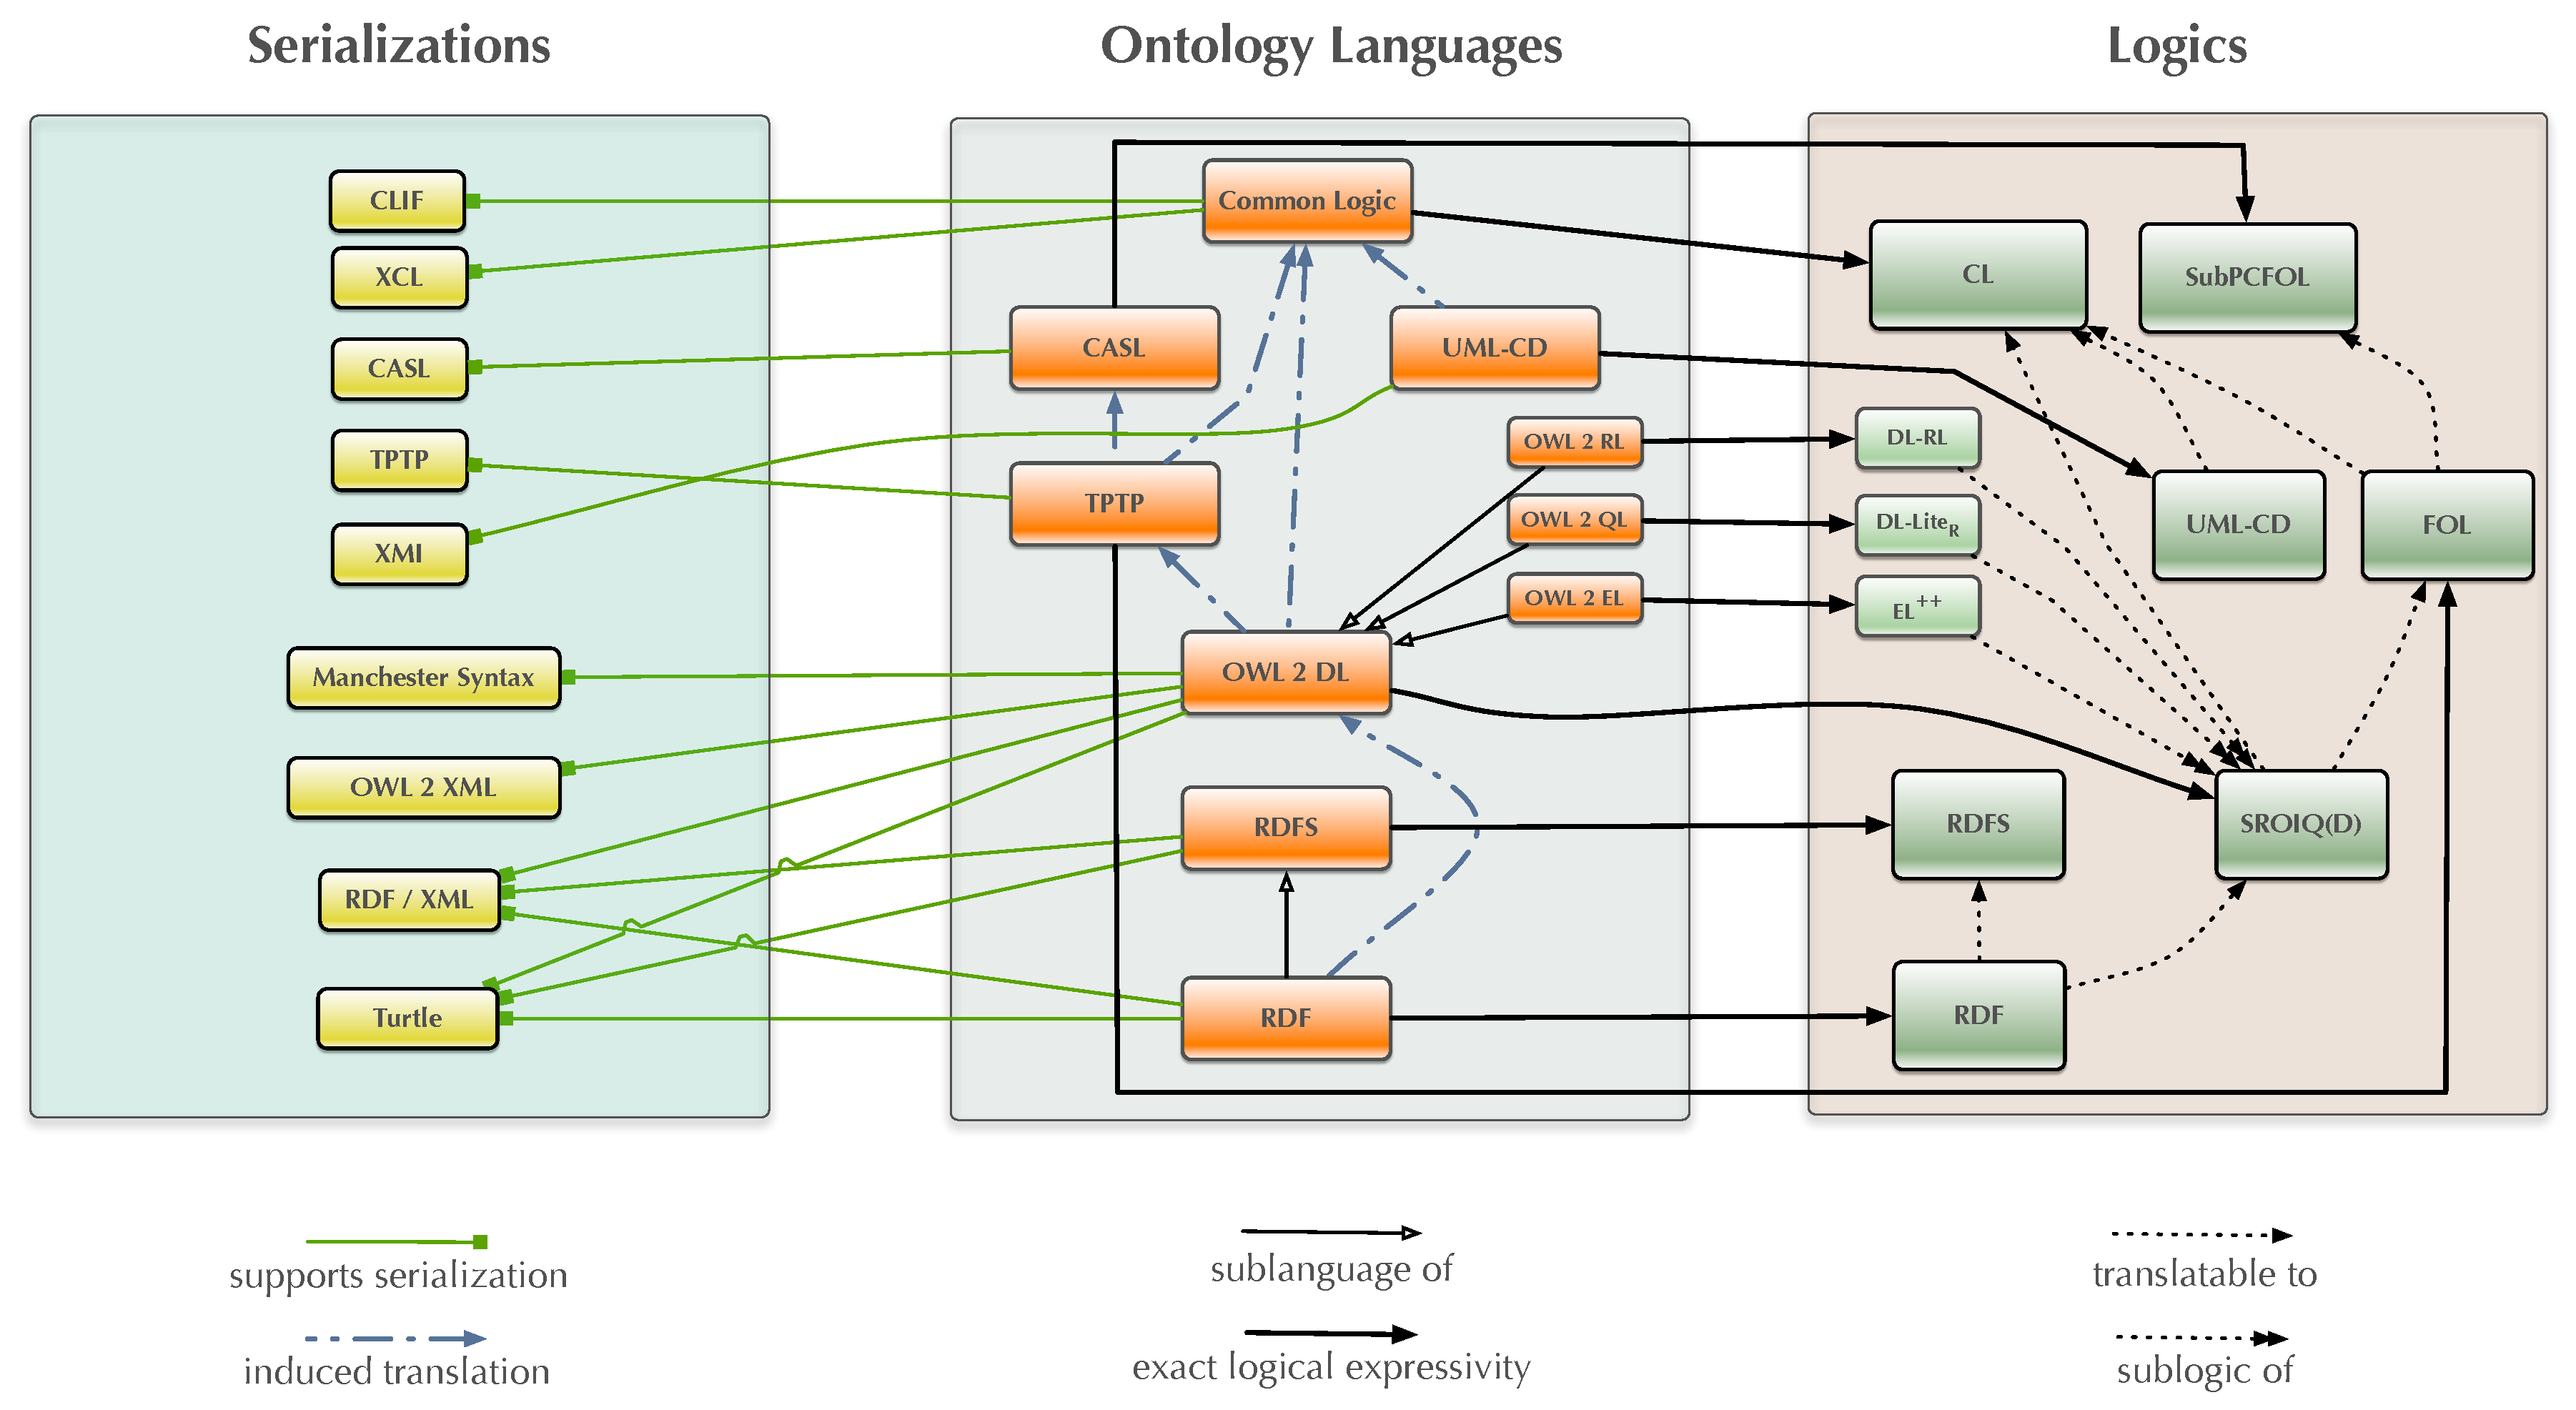
\includegraphics[width=\textwidth]{illustrations/DOL-ontograph-layers-OMG}
% %  \caption{Subset of the OntoIOp registry, shown as an RDF graph}
% %\label{f:DOL-threelayers}
% %\end{figure}
%
% This annex specifies the \DOL Ontology, an RDF vocabulary that implements the terms and definitions from \cref{terms-and-defs}.
% Part of the background and design considerations of the \DOL Ontology can be found in~\cite{LMK:LoLaModularOntologyLogLangTrans12}.
%
% \sclause{Normative State and Normative References}\label{a:dol-onto-norm}
%
%
% The canonical namespace IRI for the \DOL Ontology is \url{http://www.omg.org/spec/DOL/dol-language/}.
% Normative snapshots of the implementation are published there.
% The IRI for the version of the \DOL Ontology that corresponds to this version of the OMG standard is \url{http://www.omg.org/spec/DOL/20150801/dol-language/}.
%
% The \DOL Ontology is currently implemented in OWL 2 (\nisref{W3C/TR REC-owl2-syntax:2012}).
% The normative snapshots are encoded in RDF/XML using the OWL 2 mapping to RDF graphs (\nisref{W3C/TR REC-owl2-mapping-to-rdf:2012}).
%
% The ontology makes use of the following standard ontologies and vocabularies:
% \begin{itemize}
% \item DCMI Metadata Terms (\nisref{DCMI Metadata Terms:2012})
% \item OMG Specification Metadata (SM) Vocabulary (\nisref{OMG Specification Metadata:2014})
% \item SKOS (\nisref{W3C/TR REC-skos-reference:2009})
% \end{itemize}
%
% %The sources of the \DOL ontology are being maintained in OWL Manchester
% % syntax~\cite{W3C:NOTE-owl2-manchester-syntax-20091027} at
% % \url{https://ontohub.org/meta/dol-ontology.omn}.
%
% It is intended to implement future versions of the \DOL ontology as a DOL document in \DOL.
%
% \sclause{Intended Applications of the \DOL Ontology}\label{a:dol-onto-app}
%
% Applications of the \DOL Ontology include modeling statements about OMS in RDF, e.g., when annotating OMS, or when describing new conforming logics, OMS languages, serializations, translations, etc., in the \termref{registry} of \DOL-conforming languages and translations
% (see annex~\ref{a:registry}).
%
% The DOL ontology will also be used by the API for Knowledge Platforms
% (API4KP) OMG standardization initiative, see
% \url{http://www.omgwiki.org/API4KB}, as part of their larger ontology.
%
% \sclause{Classes and Object Properties of the \DOL Ontology}\label{a:dol-onto-tables}
%
%
% The classes in the \DOL Ontology (and their annotations) correspond to the terms (and their definitions) in \cref{terms-and-defs}. This includes most of the classes used in the \DOL metamodel, but also terms used in the \DOL semantics.
%  Classes that are reifications of relations also have been introduced as object properties.  All classes and object properties are assumed to be in the \DOL Ontology namespace unless stated otherwise.
% The \DOL Ontology additionally contains some top-level abstract classes
% as shown in Fig.~\ref{fig:dol-onto-classes}.
%
% \begin{figure}
%   \centering
%     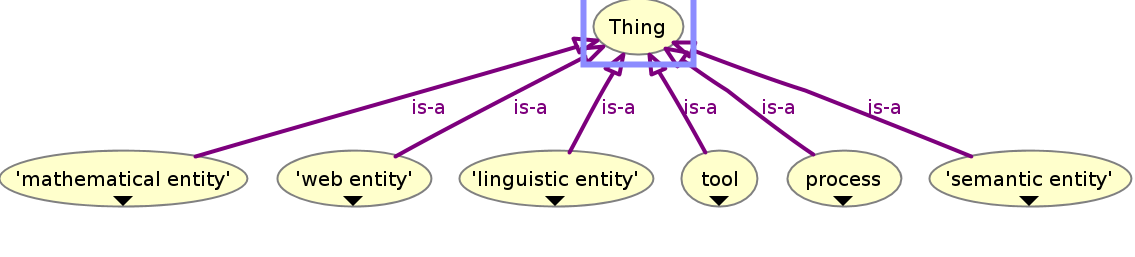
\includegraphics[width=0.8\textwidth]{illustrations/dol-onto-classes.png}
%   \caption{DOL term ontology: top-level classes}
%   \label{fig:dol-onto-classes}
% \end{figure}
%
%
%
% This reflects central issues in the structure of \DOL:
% while \DOL, as a language, is a linguistic entity, it is
% related to mathematical entities like logics, signatures and models
% through its semantics. That is, semantic entities provide the
% bridge bewteen linguistic and mathematical entities.
% Moreover, processes (like theorem proving) provide algorithmic
% procedcures for manipulating DOL librares, and tools implement
% these in software.
%
% Below the top-level classes, the class structure is as shown
% in Figs.~\ref{fig:linguistic-entity}--\ref{fig:tool}.
%
% %\includegraphics[width=0.8\textwidth]{illustrations/linguistic-entity2.png}
%
% \begin{figure}
%   \centering
%     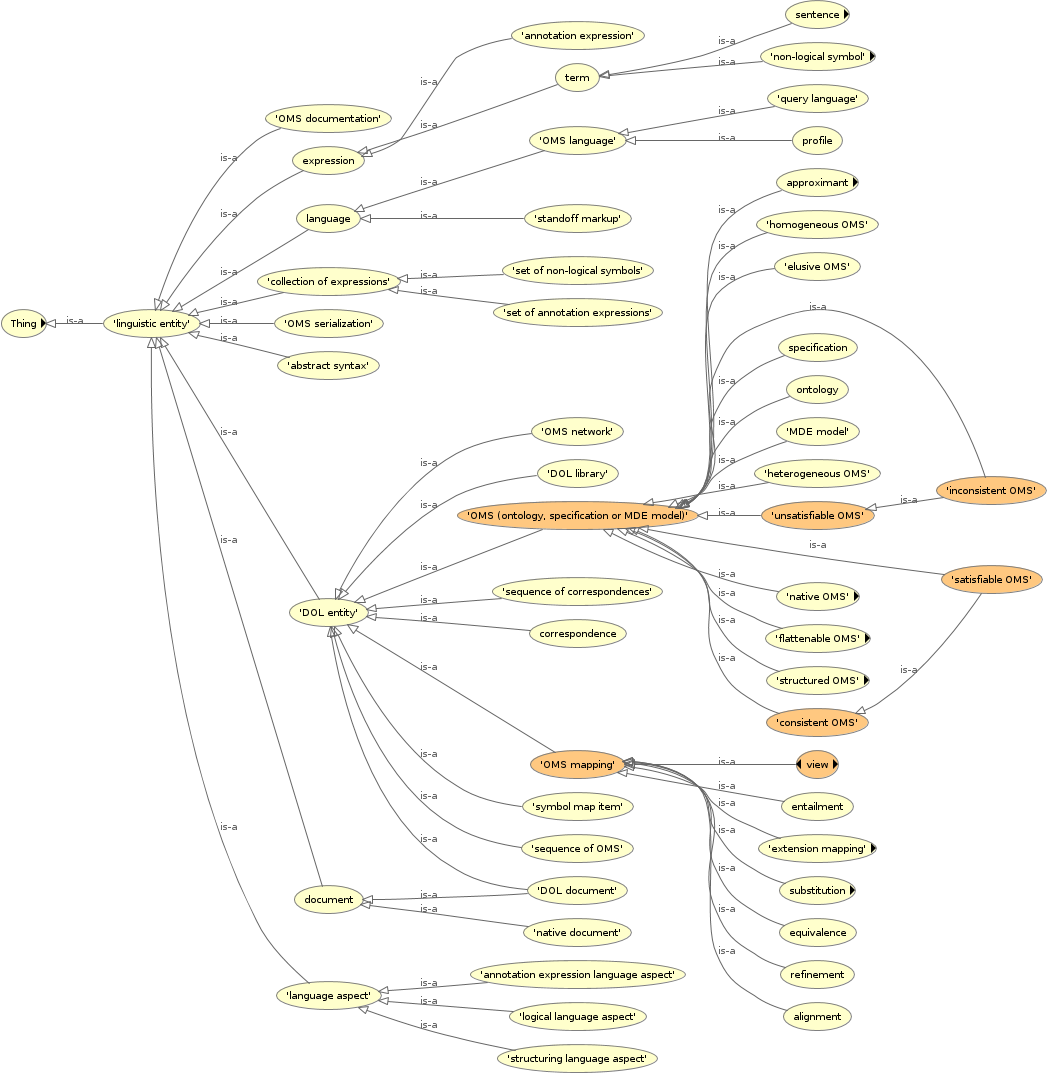
\includegraphics[width=1\textwidth]{illustrations/linguistic-entity.png}
%   \caption{DOL term ontology: linguistic entities}
%   \label{fig:linguistic-entity}
% \end{figure}
%
% \begin{figure}
%   \centering
%     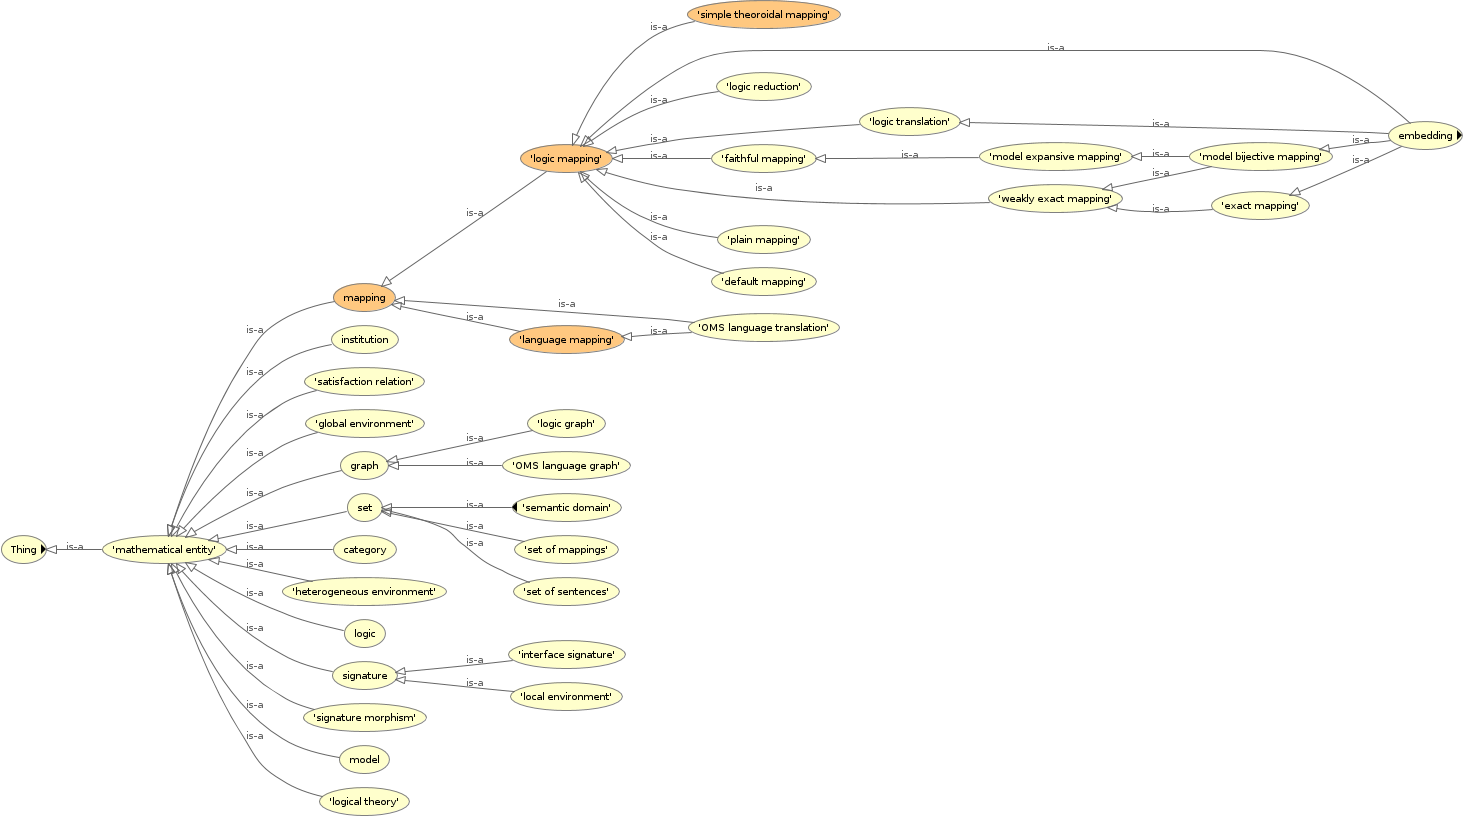
\includegraphics[width=1\textwidth]{illustrations/mathematical-entity.png}
%   \caption{DOL term ontology: mathematical entities}
%   \label{fig:mathematical-entity}
% \end{figure}
%
% \begin{figure}
%   \centering
%     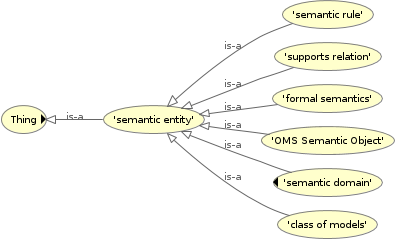
\includegraphics[width=0.4\textwidth]{illustrations/semantic-entity.png}
%   \caption{DOL term ontology: semantic entities}
%   \label{fig:semantic-entity}
% \end{figure}
%
%
% \begin{figure}
%   \centering
%     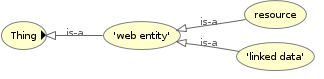
\includegraphics[width=0.4\textwidth]{illustrations/web-entity.png}
%   \caption{DOL term ontology: web entities}
%   \label{fig:web-entity}
% \end{figure}
%
%
% \begin{figure}
%   \centering
%     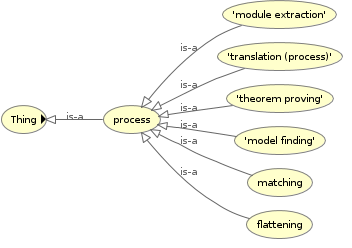
\includegraphics[width=0.4\textwidth]{illustrations/process.png}
%   \caption{DOL term ontology: processes}
%   \label{fig:process}
% \end{figure}
%
%
% \begin{figure}
%   \centering
%     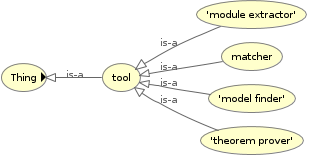
\includegraphics[width=0.4\textwidth]{illustrations/tool.png}
%   \caption{DOL term ontology: tools}
%   \label{fig:tool}
% \end{figure}
%
%
%
%
% The top level object properties are structured in a way similar
% to that of the top-level classes, see Fig.~\ref{fig:dol-onto-properties}.
% \medskip
%
% \begin{figure}
%   \centering
%     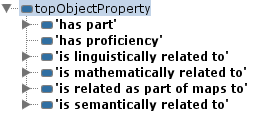
\includegraphics[width=0.4\textwidth]{illustrations/dol-onto-properties.png}
%   \caption{DOL term ontology: properties}
%   \label{fig:dol-onto-properties}
% \end{figure}
%
%



% %  \ednote{This paragraph has merely been moved.}
% It is expected that \DOL will be used for other languages than the  set of \DOL-conforming
% languages that are discussed in this \IS. OMG hosts a
% \textbf{\termref{registry} for
%  \DOL-conforming languages and translations}.
% %
% %There is a  \textbf{\termref{registry} for
% %\DOL-conforming languages and translations} hosted
% %at \url{http://purl.net/DOL/registry}.
% The registry  also includes descriptions of
% \DOL-conforming languages and translations (as well as other information needed by implementors
% and users) in both human-readable and machine-processable form.
%
% %There will be Maintenance Authority (MA) {or, depending on advisability, a Registration
% %Authority} established to
%
% OMG maintains the registry as an informative resource governed by the
% standard.  The registry contents itself is informative.
% %will not be normative; however, it is
% %



\cleardoublepage

\infannex{Conformance of OWL 2 DL With \DOL}\label{a:owl}
\sclause{General}
\CLnote{Is it correct that ``With'' and ``of'' use different capitalizations?}%
\CLnote{Why refer to this external paper when \SROIQ is actually formalized as an institution below?  Maybe cut this sentence and replace it by a general introduction?  Or at least rephrase ``is established'' into ``has originally been established''.}%
The semantic conformance of OWL 2 DL (as specified in \nisref{W3C/TR REC-owl2-syntax:2012}) with \DOL
is established in \cite{OntoGraph}.


%%%%%%%%%%%%%%%%%%%%%%%%%%%%%%%%%%%%%%%%%%%%%%%%%%%%%%%%%%%%%%%%%%%%%%%%%%%%%%%%%%%%%%%%%%%%%%%%%%%%%%%%%%%%%%%%%%%%%%%%%%%%%%%%%%
%%%%%%%%%%%%%%%%%%%%%%%%%%%%%%%%%%%%%%%%%%%%%%%%%%%%%%%%%%%%%%%%%%%%%%%%%%%%%%%%%%%%%%%%%%%%%%%%%%%%%%%%%%%%%%%%%%%%%%%%%%%%%%%%%%

\sclause{Abstract Syntax Conformance of OWL 2 With \DOL}

The metaclass \syntax{OWLOntology}~\nref{ODM}, 11.2 is a subclass (in the sense of SMOF
multiple classification) of \syntax{NativeDocument}.
The metaclass \syntax{OWLUniverse}~\nref{ODM}, 11.7 is a subclass (in the sense of SMOF
multiple classification) of \syntax{BasicOMS}.

%%%%%%%%%%%%%%%%%%%%%%%%%%%%%%%%%%%%%%%%%%%%%%%%%%%%%%%%%%%%%%%%%%%%%%%%%%%%%%%%%%%%%%%%%%%%%%%%%%%%%%%%%%%%%%%%%%%%%%%%%%%%%%%%%%
%%%%%%%%%%%%%%%%%%%%%%%%%%%%%%%%%%%%%%%%%%%%%%%%%%%%%%%%%%%%%%%%%%%%%%%%%%%%%%%%%%%%%%%%%%%%%%%%%%%%%%%%%%%%%%%%%%%%%%%%%%%%%%%%%%

\sclause{Conformance of the OWL Serializations With \DOL}\label{a:owl-serializations}

%%%%%%%%%%%%%%%%%%%%%%%%%%%%%%%%%%%%%%%%%%%%%%%%%%%%%%%%%%%%%%%%%%%%%%%%%%%%%%%%%%%%%%%%%%%%%%%%%%%%%%%%%%%%%%%%%%%%%%%%%%%%%%%%%%


\ssclause{Text Conformance of the OWL 2 Manchester Syntax With \DOL}

The OWL 2 Manchester syntax satisfies the criteria for text conformance established in clause~\ref{c:conform:serialization} in a straightforward way thanks to its line-based comment syntax (comments starting with \texttt{\#}) and its flexible handling of line breaks.


%%%%%%%%%%%%%%%%%%%%%%%%%%%%%%%%%%%%%%%%%%%%%%%%%%%%%%%%%%%%%%%%%%%%%%%%%%%%%%%%%%%%%%%%%%%%%%%%%%%%%%%%%%%%%%%%%%%%%%%%%%%%%%%%%%

\ssclause{Conformance of the XML and RDF Serializations of OWL With \DOL}\label{sec:conformance-owl-xml-rdf}

%%%%%%%%%%%%%%%%%%%%%%%%%%%%%%%%%%%%%%%%%%%%%%%%%%%%%%%%%%%%%%%%%%%%%%%%%%%

\sssclause{General Issues}

With minor modifications detailed below, the OWL/XML serialization~\cite{W3C:REC-owl2-xml-serialization-20121211} satisfies the criteria for XML conformance and the serialization of OWL in RDF (\nref{OWL2RDF}) satisfies RDF the criteria for RDF conformance. %~\CLnote{also need conformance propositional logic; use PL ``profile'' of the CASL ``IFIP standard''}
Both modifications define a super-language of the respective OWL serialization.
Any OWL ontology serialization $S'$ in one of these two super-languages can be translated into an OWL ontology serialization $S$ that fully conforms to the original specification OWL/XML or ``OWL serialized in RDF'' and is semantically equivalent to the extended serialization $S'$ with regard to the semantics of OWL.
Without these modifications, neither OWL/XML nor ``OWL serialized in RDF'' satisfies the XML or RDF conformance requirements, respectively.
The reason is that with imports there is a structural element supported by OWL that cannot have identifiers nor carry annotations, and that these two OWL serializations do not permit the use of XML or RDF constructs that would enable assigning identifiers to imports.

%%%%%%%%%%%%%%%%%%%%%%%%%%%%%%%%%%%%%%%%%%%%%%%%%%%%%%%%%%%%%%%%%%%%%%%%%%%

\sssclause{XML Conformance of a Modified OWL/XML With \DOL}\label{sec:xml-conf-modif}

In the OWL/XML serialization, the \textit{Import} element does not have annotations and is only allowed to carry the attributes \textit{xml:base}, \textit{xml:lang} and \textit{xml:space}, but no further attributes or child elements from foreign namespaces (requirement (\ref{it:foreign-xml-namespaces})), and therefore in particularly not a \textit{dol:id} attribute or child elements, as would be required for adding identifiers (cf.\ clause~\ref{sec:existing-serialization}).

An extended specification of OWL/XML that does allow the \textit{dol:id} attribute on \textit{Import} satisfies the XML conformance criteria.
From an ontology serialized in this super-language of OWL/XML, one can obtain a semantically equivalent ontology (with regard to the semantics of OWL) by stripping all \textit{dol:id} attributes.

%%%%%%%%%%%%%%%%%%%%%%%%%%%%%%%%%%%%%%%%%%%%%%%%%%%%%%%%%%%%%%%%%%%%%%%%%%%

\sssclause{RDF Conformance of a Modified Serialization of OWL in RDF With \DOL}

The serialization of OWL in RDF (regardless of the concrete \emph{RDF} serialization employed to serialize the RDF graph that represents the OWL ontology) does not satisfy requirement (\ref{it:ids-for-structure}) for RDF conformance because there is an \texttt{owl:imports} property but no class representing imports. 
Therefore, it is not possible to represent a concrete import, of an ontology $O_1$ importing an ontology $O_2$, as an RDF resource.
However, only resources can have identifiers in RDF.
RDF reification would allow for turning the statement $O_1$ \texttt{owl:imports} $O_2$ into a resource and thus giving it an identifier. 
However, the RDF triples required for expressing this reification, including, e.g., the triple \texttt{:import\_id rdf:predicate owl:imports},  would not match the head of any rule in the mapping from RDF graphs to the OWL structural specification\footnote{\nref{OWL2RDF}, section 3}. 
They would thus remain left over in the RDF graph that is attempted to be parsed into an OWL ontology, and thus violate the requirement that at the end of this parsing process, the RDF graph must be empty\footnote{See the last sentence of section 3.2.5 of \nref{OWL2RDF}}.

After extending the specification of the serialization of OWL in RDF in the following way, it satisfies the RDF conformance criteria: if the input RDF graph $G$ considered in section 3 of \nref{OWL2RDF} contains the pattern

\begin{lstlisting}[basicstyle=\small\ttfamily,language=N3,mathescape]
$i$ rdf:subject $s$ .
$i$ rdf:predicate owl:imports .
$i$ rdf:object $o$ .
\end{lstlisting}

and thus introduces a resource $i$ to represent that the ontology $s$ imports the ontology $o$, these three triples are removed from $G$.
From an ontology serialized in this super-language of the serialization of OWL in RDF, one can obtain semantically equivalent ontologies (with regard to the semantics of OWL) by stripping all triples whose predicate is \textit{rdf:subject}, \textit{rdf:predicate} or \textit{rdf:object}, or by adding triples that declare these three properties to be \emph{annotation properties}.


%%%%%%%%%%%%%%%%%%%%%%%%%%%%%%%%%%%%%%%%%%%%%%%%%%%%%%%%%%%%%%%%%%%%%%%%%%%%%%%%%%%%%%%%%%%%%%%%%%%%%%%%%%%%%%%%%%%%%%%%%%%%%%%%%%
%%%%%%%%%%%%%%%%%%%%%%%%%%%%%%%%%%%%%%%%%%%%%%%%%%%%%%%%%%%%%%%%%%%%%%%%%%%%%%%%%%%%%%%%%%%%%%%%%%%%%%%%%%%%%%%%%%%%%%%%%%%%%%%%%%

\sclause{Semantic Conformance of OWL 2 With \DOL}\label{a:owl-logic}


 The logic \SROIQ underlying 
OWL can be formalized as an institution as follows:
\begin{definition}\label{DL} \defsty{OWL 2 DL.} 
\OWL~2~DL is the description logic (DL) based fragment of the web ontology language \OWL. 
 First, the simple description logic $\ALC$ is discussed, afterward the approach is generalized
to the more complex description logic \SROIQ{}, which is underlying \OWL~2~DL.
Signatures of the description logic $\ALC$ consist of a set  ${\mathcal A}$ of
atomic concepts, a set ${\mathcal R}$ of roles and a set ${\mathcal
I}$ of individual constants. Signature morphisms are tuples of
functions, one for each signature component.
Realisations are  first-order structures $I = (\Delta^I, .^I)$ with universe $\Delta^I$
that interpret concepts as unary and roles as binary predicates
(using $.^I$). $I_1\leq I_2$ if $\Delta^{I_1}=\Delta^{I_2}$ and all
concepts and roles of $I_1$ are subconcepts and subroles of those in $I_2$.
Sentences are subsumption relations $C_1\sqsubseteq C_2$ between
concepts, where concepts follow the grammar
%\CLnote[type=q-aut]{This grammar should also be adapted to ISO EBNF.}
$$C ::= {\mathcal A} \,|\, \top\,|\, \bot \,|\, C_1 \sqcup C_2 \,|\, C_1 \sqcap C_2 \,|\, \neg C 
    \,|\, \forall R . C \,|\, \exists R . C$$
These kind of sentences are also called TBox sentences.
 Sentences can also be ABox sentences, which are
membership assertions of individuals in concepts (written $a:C$ for
$a\in{\mathcal I})$ or pairs of individuals in roles (written $R(a,b)$
for $a,b\in{\mathcal I}, R\in{\mathcal R}$).   Satisfaction is the
standard satisfaction of description logics.

The logic \SROIQ \cite{SROIQ}, which is the logical core of the Web Ontology
Language \OWL 2 DL\footnote{See also \url{http://www.w3.org/TR/owl2-overview/}}, extends $\ALC$
with the following constructs: (i) complex role inclusions such as $R \circ S \sqsubseteq S$
as well as simple role hierarchies such as $R \sqsubseteq S$,
assertions for symmetric, transitive, reflexive, asymmetric and
disjoint roles (called RBox sentences, denoted by $\mathcal{SR}$), as well as the construct
$\exists R . \mathsf{Self}$ (collecting the set of `$R$-reflexive
points'); (ii) nominals, i.e.\ concepts of the form $\{a\}$, where $a\in\mathcal{I}$ (denoted by $\mathcal{O}$); (iii) inverse
roles (denoted by $\mathcal{I}$); qualified and unqualified number
restrictions ($\mathcal{Q}$). For details on the rather complex
grammatical restrictions for \SROIQ (e.g.\ regular role inclusions,
simple roles) compare \cite{SROIQ}.

\OWL \emph{profiles} are syntactic restrictions of \OWL~2~DL that support specific modeling and reasoning tasks, %\cite{w3c:owl2-profiles}, 
and which are accordingly based on DLs with appropriate computational properties. Specifically, \OWL~2~\EL is designed for ontologies containing large numbers of concepts or relations, \OWL~2~\QL to support query answering over large amounts of data, and \OWL~2~\RL to support scalable reasoning using rule languages (\EL, \QL, and \RL for short) .
 
 The logic \ELDL is underlying the \EL profile. (To be exact, \EL adds various `harmless' expressive means and syntactic sugar to \ELDL resulting in the DL \ELDL${+}{+}$.) % \cite{BaaderEtAl-OWLED08DC}; for further details see also \cite{w3c:owl2-profiles}. 
\ELDL is a syntactic restriction of \ALC to existential restriction, concept
intersection, and the top concept:
%\ednote{TM@OK: please be  a bit more precise here, perhaps write some grammar: C ::= ⊤ | A | C ⊓ D | ∃r.C, footnote about added sugar in OWL EL profile} Note that \EL is a very relevant ontology language; large medical ontologies like SNOMED\ednote{CL@TM: FYI, it's SNO not SNOW} CT are epxressed in \EL.\ednote{TM@OK: add RL and QL if there is space}
%\ednote{Text entfernt: ``I.e.\ its concepts follow the following grammar'' -- versteht sich IMHO von selbst, nachdem man das obige \ALC-Beispiel gelesen hat}
$$C ::= {\mathcal A} \,|\, \top \,|\,  C_1 \sqcap C_2 \,|\, \exists R . C$$
Note that \ELDL does not have disjunction or negation, and is therefore a sub-Boolean logic.
\qed\end{definition}



OWL itself is more complicated than \SROIQ due to the presence of datatypes.
Following the direct model-theoretic semantics of OWL \cite{w3c:owl2-direct-semantics}:

\begin{definition}
A datatype map, formalizing datatype maps from the OWL 2 Specification \cite{w3c:owl2-spec}, is a 6-tuple 
$$D = ( N_{DT} , N_{LS} , N_{FS} , \cdot^{DT} , \cdot^{LS} , \cdot^{FS} )$$ with the following components:
\begin{itemize}
\item
    $N_{DT}$ is a set of datatypes (more precisely, names of datatypes) that does not contain the datatype \textit{rdfs:Literal}.
\item
    $N_{LS}$ is a function that assigns to each datatype $DT \in N_{DT}$ a set $N_{LS}(DT)$ of strings called lexical forms. The set $N_{LS}(DT)$ is called the lexical space of $DT$.
\item
    $N_{FS}$ is a function that assigns to each datatype $DT \in N_{DT}$ a set $N_{FS}(DT)$ of pairs $( F , v )$, where $F$ is a constraining facet and $v$ is an arbitrary data value called the constraining value. The set $N_{FS}(DT)$ is called the facet space of $DT$.
\item
    For each datatype $DT \in N_{DT}$, the interpretation function $\cdot^{DT}$ assigns to $DT$ a set $(DT)^{DT}$ called the value space of DT.
\item
    For each datatype $DT \in N_{DT}$ and each lexical form $LV \in N_{LS}(DT)$, the interpretation function $\cdot^{LS}$ assigns to the pair $( LV , DT )$ a data value $( LV , DT )^{LS} \in (DT)^{DT}$.
\item
    For each datatype $DT \in N_{DT}$ and each pair $( F , v ) \in N_{FS}(DT)$, the interpretation function $\cdot^{FS}$ assigns to $( F , v )$ the set $( F , v )^{FS}\subseteq(DT)^{DT}$. 
\end{itemize}

The set of datatypes $N_{DT}$ of a datatype map $D$ is not required to contain all datatypes from the OWL 2 datatype map; this allows one to talk about subsets of the OWL 2 datatype map, which may be necessary for the various profiles of OWL 2. If, however, $D$ contains a datatype $DT$ from the OWL 2 datatype map, then $N_{LS}(DT)$, $N_{FS}(DT)$, $(DT)^{DT}$, $( LV , DT )^{LS}$ for each $LV \in N_{LS}(DT)$, and $( F , v )^{FS}$ for each $( F , v ) \in N_{FS}(DT)$ are required to coincide with the definitions for $DT$ in the OWL 2 datatype map.
\qed\end{definition}

Given two datatype maps $D = ( N_{DT} , N_{LS} , N_{FS} , \cdot^{DT} , \cdot^{LS} , \cdot^{FS} )$ and $D' = ( N'_{DT} , N'_{LS} , N'_{FS} , \cdot^{DT'} , \cdot^{LS'} , \cdot^{FS'} )$, we write $D\subseteq D'$ if $N_{DT}\subseteq N'_{DT}$, and
the other components of $D$ are restrictions (as functions) of those of $D'$.

\begin{definition}
A vocabulary $V = ( V_{C} , V_{OP} , V_{DP} , V_{I} , V_{DT} , V_{LT} , V_{FA} )$ over a datatype map $D$ is a 7-tuple consisting of the following elements:
\begin{itemize}
\item
    $V_{C}$ is a set of classes as defined in the OWL 2 Specification \cite{w3c:owl2-spec}, containing at least the classes \textit{owl:Thing} and \textit{owl:Nothing}.
\item
    $V_{OP}$ is a set of object properties as defined in the OWL 2 Specification \cite{w3c:owl2-spec}, containing at least the object properties \textit{owl:topObjectProperty} and \textit{owl:bottomObjectProperty}.
\item
    $V_{DP}$ is a set of data properties as defined in the OWL 2 Specification \cite{w3c:owl2-spec}, containing at least the data properties \textit{owl:topDataProperty} and \textit{owl:bottomDataProperty}.
\item
    $V_{I}$ is a set of individuals (named and anonymous) as defined in the OWL 2 Specification \cite{w3c:owl2-spec}.
\item
    $V_{DT}$ is a set containing all datatypes of D, the datatype \textit{rdfs:Literal}, and possibly other datatypes; that is, $N_{DT} \cup \{ \textit{rdfs:Literal} \} \subseteq V_{DT}$.
\item
    $V_{LT}$ is a set of literals $LV^{DT}$ for each datatype $DT \in N_{DT}$ and each lexical form $LV \in N_{LS}(DT)$.
\item
    $V_{FA}$ is the set of pairs $( F , lt )$ for each constraining facet $F$, datatype $DT \in N_{DT}$, and literal $lt \in V_{LT}$ such that $( F , ( LV , DT_1 )^{LS} ) \in N_{FS}(DT)$, where $LV$ is the lexical form of $lt$ and $DT_1$ is the datatype of $lt$. 
\end{itemize}
\qed\end{definition}


\begin{definition}
Given a datatype map $D$ and a vocabulary $V$ over $D$, an interpretation $$I = ( \Delta_I , \Delta_D , \cdot^{C} , \cdot^{OP} , \cdot^{DP} , \cdot^{I} , \cdot^{DT} , \cdot^{LT} , \cdot^{FA} , \mathit{NAMED} )$$ for $D$ and $V$ is a 10-tuple with the following structure:
\begin{itemize}
\item
    $\Delta_I$ is a nonempty set called the object domain.
\item
    $\Delta_D$ is a nonempty set disjoint with $\Delta_I$ called the data domain such that $(DT)^{DT} \subseteq \Delta_D$ for each datatype $DT \in V_{DT}$.
\item
    $\cdot^{C}$ is the class interpretation function that assigns to each class $C \in V_{C}$ a subset $(C)^C \subseteq \Delta_I$ such that
\begin{itemize}
\item
        $(\textit{owl:Thing})^C = \Delta_I$ and
\item
        $(\textit{owl:Nothing})^C = \emptyset$. 
\end{itemize}
\item
    $\cdot^{OP}$ is the object property interpretation function that assigns to each object property $OP \in V_{OP}$ a subset $(OP)^{OP} \subseteq \Delta_I \times \Delta_I$ such that
\begin{itemize}
\item
        $(\textit{owl:topObjectProperty})^{OP} = \Delta_I \times \Delta_I$ and
\item
        $(\textit{owl:bottomObjectProperty})^{OP} = \emptyset$. 
\end{itemize}
\item
    $\cdot^{DP}$ is the data property interpretation function that assigns to each data property $DP \in V_{DP}$ a subset $(DP)^{DP} \subseteq \Delta_I \times \Delta_D$ such that
\begin{itemize}
\item
        $(\textit{owl:topDataProperty})^{DP} = \Delta_I \times \Delta_D$ and
\item
        $(\textit{owl:bottomDataProperty})^{DP} = \emptyset$. 
\end{itemize}
\item
    $\cdot^{I}$ is the individual interpretation function that assigns to each individual $a \in V_{I}$ an element $(a)^{I} \in \Delta_I$.
\item
    $\cdot^{DT}$ is the datatype interpretation function that assigns to each datatype $DT \in V_{DT}$ a subset $(DT)^{DT} \subseteq \Delta_D$ such that
\begin{itemize}
\item
        $\cdot^{DT}$ is the same as in $D$ for each datatype $DT \in N_{DT}$, and
\item
        $(\textit{rdfs:Literal})^{DT} = \Delta_D$. 
\end{itemize}
\item
    $\cdot^{LT}$ is the literal interpretation function that is defined as $(lt)^{LT} = ( LV , DT )^{LS}$ for each $lt \in V_{LT}$, where $LV$ is the lexical form of $lt$ and $DT$ is the datatype of $lt$.
\item
    $\cdot^{FA}$ is the facet interpretation function that is defined as $( F , lt )^{FA} = ( F , (lt)^{LT} )^{FS}$ for each $( F , lt ) \in V_{FA}$.
\item
    $\mathit{NAMED}$ is a subset of $\Delta_I$ such that $(a)^{I} \in \mathit{NAMED}$ for each named individual $a \in V_{I}$. 
\end{itemize}
\qed\end{definition}

The institution $\SROIQ(D)$ underlying OWL is now defined as follows:
\begin{definition}
\begin{itemize}
\item An $\SROIQ(D)$ signature is a pair $(D,V)$, where $D$ is a
  datatype map and $V$ a vocabulary over $D$.
\item Given $\SROIQ(D)$ signatures $(D,V)$ and $(D',V')$, a
  $\SROIQ(D)$ signature morphism $\sigma\colon (D,V)\to(D',V')$ only
  exists if $D\subseteq D'$. In this case, such a signature morphism
  consists of
\begin{itemize}
\item a map $\sigma_C\colon V_{C}\to V'_{C}$,
\item a map $\sigma_{OP}\colon V_{OP}\to V'_{OP}$,
\item a map $\sigma_{DP}\colon V_{DP}\to V'_{DP}$,
\item a map $\sigma_I\colon V_{I}\to V'_{I}$,
\item a map $\sigma_{DT}\colon V_{DT}\to V'_{DT}$ that is the identity
on $N_{DT} \cup \{ \textit{rdfs:Literal} \}$,
\item a map $\sigma_{LT}\colon V_{LT}\to V'_{LT}$ 

\end{itemize}
\item The sentences for a signature are definded as in
the direct model-theoretic semantics of OWL \cite{w3c:owl2-direct-semantics}. Sentence translation is substitution of symbols.
\item  $(D,V)$-realisations are interpretations for $D$ and $V$. 
Morphisms of $(D,V)$-models are maps between the domains $\Delta_I$ preserving membership in classes and properties, where $\Delta_D$ is mapped identically. Reducts of realisations are built by first translating along the signature morphism and then
looking up the interpretation in the realisation to be reduced.  
\item The satisfaction relation is defined as in direct model-theoretic semantics of OWL \cite{w3c:owl2-direct-semantics}.
\end{itemize}
\qed\end{definition}


Remark: strictly speaking, the institution defined above is
\emph{{OWL} 2 DL without restrictions} in the sense of
\cite{DBLP:conf/owled/SchneiderRS13}. The reason is that in an
institution, the sentences can be used for arbitrary formation of
theories. This is related to the presence of \DOL's union operator on
OMS.  OWL 2 DL's specific restrictions on theory formation can be
modeled \emph{inside} this institution, as a constraint on OMS.  This
constraint is generally not preserved under unions or
extensions. \DOL's multi-logic capability allows the clean distinction
between ordinary OWL 2 DL and {OWL} 2 DL without restrictions.

%%%%%%%%%%%%%%%%%%%%%%%%%%%%%%%%%%%%%%%%%%%%%%%%%%%%%%%%%%%%%%%%%%%%%%%%%%%%%%%%%%%%%%%%%%%%%%%%%%%%%%%%%%%%%%%%%%%%%%%%%%%%%%%%%%

\ssclause{Relativization in \OWL}

\begin{definition}
Given an \OWL theory $T = ((C,R,I), \Delta)$,
the \emph{relativization} of $T$, denoted $\tilde{T}$, is the theory 
$((C',R,I),\Delta')$ where
\begin{itemize}
\item $C' = C\cup\{\top_T\}$
\item $\Delta'$ contains axioms stating that:
  \begin{itemize}
    \item each concept in $C$ is subsumed by $\top_T$,
    \item each individual in $I$ is an instance of $\top_T$,
    \item each role $r$ has its domain and range intersected with $\top_T$, if they
    are present in $\Delta$, otherwise they are $\top_T$,
  \end{itemize}
  \noindent and, for each sentence $e\in\Delta$, the sentence $\alpha(e)$, obtained by
  replacing the concepts in $e$ as follows:
  are made:
  \begin{itemize}
   \item each occurence of $\top$ is replaced with $\top_T$,
   \item each occurence of $\neg C$ is replaced with $\top_T \sqcap \neg C$,
   \item each occurence of $\forall~r\bullet C$ is replaced with 
   $\top_T \sqcap \forall~r\bullet C$.
  \end{itemize}
\end{itemize}
\end{definition}

\begin{definition}
Given an \OWL theory $T = ((C,R,I), \Delta)$,
we define $\beta: Mod^\OWL(\tilde{T}) \to Mod^\OWL(T)$ as follows: 
if $M'\in Mod^\OWL(\tilde{T})$, then $M=\beta(M')$ has as universe
$\Delta^M$ the set $(\top_T)^{M'}$ and each concept, role and individual are
interpreted in $M$ in the same way as in $M'$. Since $M'$ is a $\Delta'$-realisation,
we get that $M$ is indeed a $(C,R,I)$-realisation and moreover $M\models \Delta$.
\end{definition}

\begin{note}
If $T = ((C,R,I),\Delta)$ is an \OWL theory, $M'$ is a $\tilde{T}$-realisation and
$e$ is a $(C,R,I)$-sentence, we have that $M'\models \alpha(e)$ if and only if
$\beta(M')\models e$.
\end{note}

%%%%%%%%%%%%%%%%%%%%%%%%%%%%%%%%%%%%%%%%%%%%%%%%%%%%%%%%%%%%%%%%%%%%%%%%%%%%%%%%%%%%%%%%%%%%%%%%%%%%%%%%%%%%%%%%%%%%%%%%%%%%%%%%%%

\ssclause{Translating correspondences to a bridge theory in \OWL}

We define the function $theoryOfCorrespondences_\OWL$ that takes as arguments
the assumption made on the semantics of the alignment where the
correspondences come from, the signatures of the two ontologies being aligned
and a list of processed correspondences, in the sense 
that the default correspondence and any correspondence block, if present, 
are replaced with the lists of single correspondences they induce,
represented as triples of the form $(relation, sourceSymbol, targetSymbol)$.
The result of the function is a co-span of theories:
$\xymatrix{(\Sigma_s,\emptyset) \ar[r]^{\varphi_s} & (\Sigma,\Delta) & \ar[l]_{\varphi_t} (\Sigma_t,\emptyset)}$. Intuitively, $\Sigma_s$ and $\Sigma_t$ gather the symbols
of the aligned ontologies that appear in the list of correspondences passed as an
argument, while $(\Sigma,\Delta)$ contains an \OWL sentence 
representing each correspondence.

We distinguish three cases.
\begin{enumerate}
\item Single domain:
 \begin{itemize}
   \item no other symbols occur in the signatures $\Sigma_s$ and $\Sigma_t$
         than the ones that appear in correspondences:
         $\Sigma_s = (C_s, R_s, I_s)$ and $\Sigma_t = (C_t, R_t,I_t)$,
         where $C_s$, $R_s$ and $I_s$ are the sets of all concept names, roles
         and individuals that appear in the list of correspondences as source symbols
         and $C_t$, $R_t$ and $I_t$ are the sets of all concept names, roles
         and individuals that appear in the list of correspondences as target symbols.
  \item $\Sigma = \Sigma_s \uplus \Sigma_t$, where we prefix the symbols of 
        $\Sigma$ coming from $\Sigma_s$ with $1:$ and those coming from
        $\Sigma_t$ with $2:$
  \item $\varphi_s$ maps each symbol $s$ in $\Sigma_s$ to $1:s$
        and $\varphi_t$ maps each symbol $s$ in $\Sigma_t$ to $2:s$.
  \item $\Delta$ contains the translation of correspondences to $\Sigma$-sentences
        using the following rules:
         $$\begin{array}{ll}
            ('equivalent', c1, c2) & \verb+Class: 1:c1 EquivalentTo: 2:c2+ \\
            ('equivalent', r1, r2) & \verb+ObjectProperty: 1:r1 EquivalentTo: 2:r2+\\
            ('equivalent', i1, i2) & \verb+Individual: 1:i1 SameAs: 2:i2+\\
            ('incompatible',c1, c2)& \verb+Class: 1:c1 DisjointWith: 2:c2+ \\
            ('incompatible',r1, r2)& \verb+ObjectProperty: 1:r1 DisjointWith: 2:r2+ \\
            ('incompatible',i1, i2)& \verb+Individual: 1:i1 DifferentFrom: 2:i2+ \\
            ('subsumes',c1, c2)& \verb+Class: 2:c2 SubClassOf: 1:c1+ \\
            ('subsumes',r1, r2)& \verb+ObjectProperty: 2:r2 SubPropertyOf: 1:r1+ \\
            ('\mathit{is\text{-}subsumed}',c1, c2)& \verb+Class: 1:c1 SubClassOf: 2:c2+ \\
            ('\mathit{is\text{-}subsumed}',r1, r2)& \verb+ObjectProperty: 1:r1 SubPropertyOf: 2:r2+  \\
            ('\mathit{has\text{-}instance}', c1, i2) & \verb+Individual: 2:i2 Types: 1:c1+\\
            ('\mathit{instance\text{-}of}', i1, c2) & \verb+Individual: 1:i1 Types: 2:c2+
          \end{array}$$         
 \end{itemize}
\item Global domain: 
  \begin{itemize}
   \item 
         $\Sigma_s = (C_s\cup{\top_s}, R_s, I_s)$ and $\Sigma_t = (C_t\cup{\top_t}, R_t,I_t)$,
         where $C_s$, $R_s$ and $I_s$ are the sets of all concept names, roles
         and individuals that appear in the list of correspondences as source symbols
         and $C_t$, $R_t$ and $I_t$ are the sets of all concept names, roles
         and individuals that appear in the list of correspondences as target symbols.
  \item $\Sigma = \Sigma_s \uplus \Sigma_t$, where we prefix the symbols of 
        $\Sigma$ coming from $\Sigma_s$ with $1:$ and those coming from
        $\Sigma_t$ with $2:$
  \item $\varphi_s$ maps each symbol $s$ in $\Sigma_s$ to $1:s$
        and $\varphi_t$ maps each symbol $s$ in $\Sigma_t$ to $2:s$.
  \item $\Delta$ is constructed in the same way as in the previous case, except
        that if \verb+Thing+ appears in a correspondence, it is replaced by
        $\top_s$ or $\top_t$.\footnote{An extension of the language where complex concepts are allowed in alignments would make the construction of $\Delta$ in this
        case substantially different to the one in the previous case.} 
  \end{itemize}
        \item Contextualized domain:
 \begin{itemize}
   \item $\Sigma_s$ and $\Sigma_t$ are constructed as before, but now they also
         include the relativized top concepts $\top_S$ and $\top_T$ respectively.
   \item $\Sigma$ extends the disjoint union $\Sigma_s \uplus \Sigma_t$ with 
         new roles $r_{st}$ and $r_{ts}$.
   \item $\Delta$ contains the following axioms: 
          $$ \verb+ObjectProperty: + r_{st}~ \verb+Domain:+ \top_S~ \verb+Range:+ \top_T$$
          and 
          $$ \verb+ObjectProperty: + r_{ts}~ \verb+Domain:+ \top_T~ \verb+Range:+ \top_S$$
          together with the property that $r_{st}$ is the converse of $r_{ts}$:
          $$\verb+ObjectProperty: + r_{st} \verb+ InverseOf: + r_{ts}$$
          and translation of correspondences to $\Sigma$-sentences
        using the following rules:\ednote{
        6 - should we require that its not the case that
        $1:i1~r_{st}~2:i2$ and $2:i2~r_{ts}~1:i1$? }
         $$\begin{array}{ll}
            ('equivalent', c1, c2) & \verb+Class: 1:c1 EquivalentTo: + r_{st}\verb+ some 2:c2+ \\
            ('equivalent', r1, r2) & \verb+ObjectProperty: 1:r1 EquivalentTo: + r_{st} \verb+ o 2:r2 o + r_{ts}\\
            ('equivalent', i1, i2) & \verb+Individual: 1:i1 Facts: + r_{st} \verb+ 2:i2+\\
            ('incompatible',c1, c2)& \verb+EquivalentClasses: + 1:c1 \verb+ and + 
            r_{st} \verb+ some 2:c2, Nothing+\\
            ('incompatible',r1, r2)& \verb+ObjectProperty: 1:r1 DisjointWith: + r_{st} \verb+ o 2:r2 o + r_{ts}\\
            ('incompatible',i1, i2)& \verb+Individual: 1:i1 DifferentFrom: 2:i2+ \\
            ('subsumes',c1, c2)& \verb+Class: 2:c2 SubClassOf:  + r_{sz}\verb+ some 1:c1+ \\
            ('subsumes',r1, r2)& \verb+ObjectProperty: 2:r2 SubPropertyTo: + r_{ts} \verb+ o 1:r1 o + r_{st}\\
            ('\mathit{is\text{-}subsumed}',c1, c2)& \verb+Class: 1:c1 SubClassOf: + r_{ts}\verb+ some 2:c2+ \\
            ('\mathit{is\text{-}subsumed}',r1, r2)& \verb+ObjectProperty: 1:r1 SubPropertyTo: + r_{st} \verb+ o 2:r2 o + r_{ts} \\
            ('\mathit{has\text{-}instance}', c1, i2) & \verb+Individual: 2:i2 Types: + r_{ts}\verb+ some 1:c1+\\
            ('\mathit{instance\text{-}of}', i1, c2) & \verb+Individual: 1:i1 Types: + r_{st}\verb+ some 2:c2+
          \end{array}$$  
          Note that we must express equivalences where role compositions are involved.
          This is only possible in \OWL 2 Full. Thus the diagram returned by the function
          $\mathit{theoryOfCorrespondences}$ becomes heterogeneous:
          $$\xymatrix{ (\OWL,\Sigma_s,\emptyset) \ar[rrr]^{(OWL2Full, \varphi_s)} &&& (\OWL_{\mathit{FULL}}),\Sigma,\Delta) &&&(\OWL,\Sigma_t,\emptyset)\ar[lll]_{(OWL2Full, \varphi_t)} }$$
         \noindent                   
          where $OWL2Full$ is the inclusion comorphism of \OWL in \OWL 2 Full,
          $\varphi_s$  maps each symbol $s$ to $1:s$ and $\top_s$ to itself, 
          and $\varphi_t$  maps each symbol $t$ to $2_t$ and $\top_t$ to itself.
 \end{itemize}
\end{enumerate}


%%%%%%%%%%%%%%%%%%%%%%%%%%%%%%%%%%%%%%%%%%%%%%%%%%%%%%%%%%%%%%%%%%%%%%%%%%%%%%%%%%%%%%%%%%%%%%%%%%%%%%%%%%%%%%%%%%%%%%%%%%%%%%%%%%
%%%%%%%%%%%%%%%%%%%%%%%%%%%%%%%%%%%%%%%%%%%%%%%%%%%%%%%%%%%%%%%%%%%%%%%%%%%%%%%%%%%%%%%%%%%%%%%%%%%%%%%%%%%%%%%%%%%%%%%%%%%%%%%%%%
%%%%%%%%%%%%%%%%%%%%%%%%%%%%%%%%%%%%%%%%%%%%%%%%%%%%%%%%%%%%%%%%%%%%%%%%%%%%%%%%%%%%%%%%%%%%%%%%%%%%%%%%%%%%%%%%%%%%%%%%%%%%%%%%%%
\cleardoublepage
\infannex{Conformance of Common Logic with \DOL}\label{a:cl}

%%%%%%%%%%%%%%%%%%%%%%%%%%%%%%%%%%%%%%%%%%%%%%%%%%%%%%%%%%%%%%%%%%%%%%%%%%%%%%%%%%%%%%%%%%%%%%%%%%%%%%%%%%%%%%%%%%%%%%%%%%%%%%%%%%
%%%%%%%%%%%%%%%%%%%%%%%%%%%%%%%%%%%%%%%%%%%%%%%%%%%%%%%%%%%%%%%%%%%%%%%%%%%%%%%%%%%%%%%%%%%%%%%%%%%%%%%%%%%%%%%%%%%%%%%%%%%%%%%%%%

\sclause{Abstract Syntax Conformance of Common Logic With \DOL}

The metaclass \syntax{Text}~\nref{ODM}, 12.2 is a subclass (in the sense of SMOF \nref{SMOF}
multiple classification) of \syntax{NativeDocument}.
The metaclass \syntax{Sentence}~\nref{ODM}, 12.2 is a subclass (in the sense of SMOF \nref{SMOF}
multiple classification) of \syntax{BasicOMS}.

%%%%%%%%%%%%%%%%%%%%%%%%%%%%%%%%%%%%%%%%%%%%%%%%%%%%%%%%%%%%%%%%%%%%%%%%%%%%%%%%%%%%%%%%%%%%%%%%%%%%%%%%%%%%%%%%%%%%%%%%%%%%%%%%%%
%%%%%%%%%%%%%%%%%%%%%%%%%%%%%%%%%%%%%%%%%%%%%%%%%%%%%%%%%%%%%%%%%%%%%%%%%%%%%%%%%%%%%%%%%%%%%%%%%%%%%%%%%%%%%%%%%%%%%%%%%%%%%%%%%%

\sclause{Serialization Conformance of Common Logic With \DOL}

The semantic conformance of Common Logic (as specified in \nref{CL}) with \DOL is established in \cite{OntoGraph}.

The XCF dialect of Common Logic has a serialization that satisfies the criteria for XML conformance.  The CLIF dialect of Common Logic has a serialization that satisfies the criteria for text conformance.

\sclause{Semantic Conformance of Common Logic With \DOL}

Common Logic can be defined as an institution as follows:

\begin{definition}\label{CommonLogic} \defsty{Common Logic.}  
A common logic signature
$\Sigma$ (called vocabulary in Common Logic terminology) consists of a
set of names, with a subset called the set of discourse names, and a
set of sequence markers. An signature morphism maps
names and sequence markers separately, subject to the requirement
 that a name is a discourse
name in the smaller signature if and only if it is one in the larger signature.  A $\Sigma$-realisation $I=(\UR,\UD,\rel,\fun,\intCL,\seq)$ consists of a set $\UR$,
the universe of reference, with a non-empty subset $\UD\subseteq \UR$,
the universe of discourse, and four mappings:
  \begin{itemize}
   \item $\rel$ from $\UR$ to subsets of $\UD^* = \{ \langle x_1,\ldots,x_n\rangle \mid
x_1,\ldots,x_n \in \UD\}$ (i.e., the set of finite sequences of
elements of $\UD$);
   \item $\fun$ from $\UR$ to total functions from $\UD^*$ into $\UD$;
   \item $\intCL$ from names in $\Sigma$ to $\UR$, such that
$\intCL(v)$ is in $\UD$ if and only if $v$ is a discourse name;
   \item $\seq$ from sequence markers in $\Sigma$ to $\UD^*$.
  \end{itemize}  A $\Sigma$-sentence is a first-order
sentence, where predications and function applications are written
in a higher-order like syntax: $t(s)$.
Here, $t$ is an arbitrary term, and $s$ is a sequence term, which can
be a sequence of terms $t_1\ldots t_n$, or a sequence marker.
A predication $t(s)$ is interpreted by evaluating the term $t$,
mapping it to a relation using $\rel$, and then asking whether the sequence
given by the interpretation $s$ is in this relation.  
Similarly, a function application $t(s)$ is interpreted using $\fun$.
Otherwise, interpretation of terms and formulae is as in
first-order logic. 
A further
difference to first-order logic
is the presence of sequence terms (namely sequence markers and
juxtapositions of terms), which denote sequences in $\UD^*$, with term
juxtaposition interpreted by sequence concatenation.
Note that sequences are essentially a non-first-order feature that
can be expressed in second-order logic.

Reducts of realisations are defined in the following way: 
Given a signature morphism $\sigma:\Sigma_1\to\Sigma_2$ and a $\Sigma_2$-realisation
$I_2 =$ $(\UR,\UD,$ $\rel,\fun,\intCL,\seq)$, $I\forget{\sigma}=(\UR,\UD,\rel,\fun,\intCL\circ\sigma,\seq\circ\sigma)$. 

Given two \CL realisations $I_1=(\UR_1,\UD_1,\rel_1,\fun_1,\intCL_1,\seq_1)$
and  $I_2=(\UR_2,\UD_2,\rel_2,\fun_2,\intCL_2,\seq_2)$, a homomorphism
of realisations
$h:I_1\to I_2$ is a function $h:\UR_1\to\UR_2$ such that
\begin{itemize}
\item $h$ restricts to $k:\UD_1\to\UD_2$,
\item for each $x\in\UR_1$ and $s\in\UD_1^*$, if $s\in\rel_1(x)$, then $k^*(s)\in\rel_2(h(x))$\footnote{$k^*$ is the extension of $h$ to sequences.},
\item for each $x\in\UR_1$, $k\circ\fun_1(x)=\fun_2(h(x))\circ k^*$,
\item for each name $n$ in $\Sigma$, $\intCL_2(n)=h(\intCL_1(n))$,
\item for each sequence marker $n$ in $\Sigma$, $\seq_2(n)=k^*(\seq_1(n))$.
\end{itemize}
%
%For details, see \cite{CommonLogic:oldfashioned}.
\CLminus is the restriction of \CL to sentence
without sequence markers.\qed
\end{definition}

Note that Common Logic also includes sentence formation constructs like
\texttt{cl:import}s that in \DOL terms belong to the structuring
language. They have been omitted from the institution, because
they must not occur in basic OMS. They can occur in
structured native OMS, however, and need to be flattened out
in order to obtain a theory in the \CL institution.


%%%%%%%%%%%%%%%%%%%%%%%%%%%%%%%%%%%%%%%%%%%%%%%%%%%%%%%%%%%%%%%%%%%%%%%%%%%%%%%%%%%%%%%%%%%%%%%%%%%%%%%%%%%%%%%%%%%%%%%%%%%%%%%%%%
%%%%%%%%%%%%%%%%%%%%%%%%%%%%%%%%%%%%%%%%%%%%%%%%%%%%%%%%%%%%%%%%%%%%%%%%%%%%%%%%%%%%%%%%%%%%%%%%%%%%%%%%%%%%%%%%%%%%%%%%%%%%%%%%%%
%%%%%%%%%%%%%%%%%%%%%%%%%%%%%%%%%%%%%%%%%%%%%%%%%%%%%%%%%%%%%%%%%%%%%%%%%%%%%%%%%%%%%%%%%%%%%%%%%%%%%%%%%%%%%%%%%%%%%%%%%%%%%%%%%%
\cleardoublepage
\infannex{Conformance of RDF and RDF Schema with \DOL}\label{a:rdfs}

%%%%%%%%%%%%%%%%%%%%%%%%%%%%%%%%%%%%%%%%%%%%%%%%%%%%%%%%%%%%%%%%%%%%%%%%%%%%%%%%%%%%%%%%%%%%%%%%%%%%%%%%%%%%%%%%%%%%%%%%%%%%%%%%%%
%%%%%%%%%%%%%%%%%%%%%%%%%%%%%%%%%%%%%%%%%%%%%%%%%%%%%%%%%%%%%%%%%%%%%%%%%%%%%%%%%%%%%%%%%%%%%%%%%%%%%%%%%%%%%%%%%%%%%%%%%%%%%%%%%%

\sclause{Abstract Syntax Conformance of RDF and RDF Schema  With \DOL}

The metaclass \syntax{rdfDocument}~\nref{ODM}, 14.2.2 is a subclass (in the sense of SMOF \nref{SMOF}
multiple classification) of \syntax{NativeDocument}.
The metaclass \syntax{graph}~\nref{ODM}, 14.2.3 is a subclass (in the sense of SMOF \nref{SMOF}
multiple classification) of \syntax{BasicOMS}.


%%%%%%%%%%%%%%%%%%%%%%%%%%%%%%%%%%%%%%%%%%%%%%%%%%%%%%%%%%%%%%%%%%%%%%%%%%%%%%%%%%%%%%%%%%%%%%%%%%%%%%%%%%%%%%%%%%%%%%%%%%%%%%%%%%
%%%%%%%%%%%%%%%%%%%%%%%%%%%%%%%%%%%%%%%%%%%%%%%%%%%%%%%%%%%%%%%%%%%%%%%%%%%%%%%%%%%%%%%%%%%%%%%%%%%%%%%%%%%%%%%%%%%%%%%%%%%%%%%%%%

\sclause{Serialization Conformance of RDF and RDF Schema  With \DOL}

The way of representing RDF Schema ontologies as RDF graphs satisfies
the criteria for RDF conformance.

\sclause{Semantic Conformance of RDF and RDF Schema  With \DOL}

The semantic conformance of RDF Schema (as specified in \nref{RDFS}) 
with \DOL is established in \cite{OntoGraph}.

\begin{definition}[\RDF and RDF Schema]
The institutions for the Resource Description Framework (\RDF) and \RDF
Sche\-ma (also known as \RDFS), respectively, are defined in the
following~\cite{Lucanu}. Both \RDF and \RDFS are based on a logic called
\emph{bare} \RDF (\SimpleRDF), which consists of triples only (without
any predefined resources).

%%%%%%%%%%
A \textit{signature} $\mathbf{R_s}$ in \SimpleRDF is a set of
\textit{resource references}. For $sub, pred, obj \in \mathbf{R_s}$, a
triple of the form $(sub, pred, obj)$ is a \textit{sentence} in \SimpleRDF,
where $sub$, $pred$, $obj$ represent subject name, predicate name,
object name, respectively. An $\mathbf{R_s}$-realisation $M =
\langle R_m, P_m, S_m, EXT_m \rangle$ consists of a \textit{set $R_m$
  of resources}, a set $P_m \subseteq R_m$ of predicates, a
\textit{mapping function} $S_m:\mathbf{R_s} \rightarrow R_m$, and an
\textit{extension function} $EXT_m: P_m \rightarrow \mathcal{P}(R_m
\times R_m)$ mapping every predicate to a set of pairs of
resources. Satisfaction is defined as follows:
%
\[\mathfrak{M} \models_{\mathbf{R_s}} (sub, pred, obj) \Leftrightarrow (S_{m}(sub),
(S_{m}(obj)) \in EXT_{m} (S_m(pred)). \]
%%%%%
%
Both \RDF and \RDFS are built on top of \SimpleRDF by fixing a certain
standard vocabulary both as part of each signature and in the realisations.\ednote{Refer to the RDF standard here.}

Actually, the standard vocabulary is given by a certain theory. In case
of \RDF, it contains e.g.\ resources \texttt{rdf:type} and
\texttt{rdf:Property} and \texttt{rdf:subject}, and sentences like, e.g.
%
\begin{gather*}
  (\texttt{rdf:type},\texttt{rdf:type},\texttt{rdf:Property})
\ \text{, and}\\
  (\texttt{rdf:subject}, \texttt{rdf:type},\texttt{rdf:Property})
\ \text{.}
\end{gather*}

In the realisations, the standard vocabulary is interpreted with a fixed
realisation.  Moreover, for each $\RDF$-realisation
$M = \langle R_m, P_m, S_m,\allowbreak \mathit{EXT}_m\rangle$,
if $p\in P_m$,
then it must hold
$(p, S_m(\texttt{rdf:Property})) \in \mathit{EXT}_m(\texttt{rdf:type})$.
For \RDFS, similar conditions are formulated (here, for example also the
subclass relation is fixed).

In the case of \RDFS, the standard vocabulary contains more elements,
like \texttt{rdfs:domain}, \texttt{rdfs:range}, \texttt{rdfs:Resource},
\texttt{rdfs:Literal}, \texttt{rdfs:Datatype}, \texttt{rdfs:Class},
\texttt{rdfs:subClassOf}, \texttt{rdfs:subPropertyOf},
\texttt{rdfs:member}, \texttt{rdfs:} \texttt{Container},
\texttt{rdfs:ContainerMembershipProperty}.

There is also \OWL Full, an extension of \RDFS with resources
such as \texttt{owl:Thing} and \texttt{owl:oneOf}, tailored towards the representation of
\OWL~\cite{W3C:REC-owl2-rdf-based-semantics-20091027}.
\qed\end{definition}

%%%%%%%%%%%%%%%%%%%%%%%%%%%%%%%%%%%%%%%%%%%%%%%%%%%%%%%%%%%%%%%%%%%%%%%%%%%%%%%%%%%%%%%%%%%%%%%%%%%%%%%%%%%%%%%%%%%%%%%%%%%%%%%%%%
%%%%%%%%%%%%%%%%%%%%%%%%%%%%%%%%%%%%%%%%%%%%%%%%%%%%%%%%%%%%%%%%%%%%%%%%%%%%%%%%%%%%%%%%%%%%%%%%%%%%%%%%%%%%%%%%%%%%%%%%%%%%%%%%%%
%%%%%%%%%%%%%%%%%%%%%%%%%%%%%%%%%%%%%%%%%%%%%%%%%%%%%%%%%%%%%%%%%%%%%%%%%%%%%%%%%%%%%%%%%%%%%%%%%%%%%%%%%%%%%%%%%%%%%%%%%%%%%%%%%%
\cleardoublepage
\infannex{Conformance of UML class and object models with \DOL}\label{a:uml-class}

\sclause{General}
This informative annex demonstrates conformance of a subset of UML
class and object models with \DOL by defining an institution for
both.  The subset is restricted to the static aspects of class
models; that is, change of state is ignored. This means that all
operations are query operations.


%%%%%%%%%%%%%%%%%%%%%%%%%%%%%%%%%%%%%%%%%%%%%%%%%%%%%%%%%%%%%%%%%%%%%%%%%%%%%%%%%%%%%%%%%%%%%%%%%%%%%%%%%%%%%%%%%%%%%%%%%%%%%%%%%%
%%%%%%%%%%%%%%%%%%%%%%%%%%%%%%%%%%%%%%%%%%%%%%%%%%%%%%%%%%%%%%%%%%%%%%%%%%%%%%%%%%%%%%%%%%%%%%%%%%%%%%%%%%%%%%%%%%%%%%%%%%%%%%%%%%

\sclause{Abstract Syntax Conformance of UML With \DOL}

The metaclass \syntax{Package}~\nref{UML} is a subclass (in the sense of SMOF \nref{SMOF}
multiple classification) of \syntax{NativeDocument}.
The metaclass \syntax{PackageableElement}~\nref{UML} is a subclass (in the sense of SMOF \nref{SMOF}
multiple classification) of \syntax{BasicOMS}.

\sclause{Serialization Conformance of UML With \DOL}

The XMI \nref{XMI} serialization, derived from the MOF metamodel, is widely used
for UML. Hence, UML is serialization conformant with \DOL.

\sclause{Semantic Conformance of UML With \DOL}

The institution of UML class and object models is defined using a
translation of UML class models to Common Logic, following the fUML
specification and \cite{Seidewitz08}.

\ssclause{Preliminaries}


 The axioms for primitive types
are imported from the fUML specification, section 10.3.1:
Booleans, numbers, sequences and strings.  These
axiomatize (among others) predicates corresponding to primitive types,
e.g.\ \texttt{buml:Boolean}, \texttt{form:Number},
\texttt{form:NaturalNumber}, \texttt{buml:Integer},
\texttt{form:Sequence}, \texttt{form:Character}, and
\texttt{buml:String}.

The following infrastructure, consisting off a number of predicates
axiomatized in Common Logic, provides a foundation for an institution
for UML class models described in the later sections of this Annex.
%
\begin{lstlisting}[language=clif, basicstyle={\ttfamily\fontsize{8pt}{9pt}\selectfont},
                   morekeywords={then, with, logic, oms, end},
                   morecomment={[l]{//}},
                   mathescape]
logic CLIF

oms pairs =
  (forall (x y) (= (form:first (form:pair x y)) x))
  (forall (x y) (= (form:second (form:pair x y)) y))
  (forall (x y) (form:Pair (form:pair x y)))
  (forall (p) (if (form:Pair p)
                  (= (form:pair (form:first p) (form:second p)) p)))
end

oms sequences =
  fuml:sequences.clif and pairs
then
  // Membership of an element in a sequence
  (forall (x s)
          (if (form:sequence-member x s)
              (form:Sequence s)))
  (forall (x s)
          (iff (form:sequence-member x s)
               (exists (p) 
                       (and (form:in-sequence s p)
                            (form:in-position p x)))))

  // Selection of elements
  (forall (o)
          (= (form:select1 o form:empty-sequence) form:empty-sequence))
  (forall (o y s)
          (= (form:select1 o (form:sequence-insert (form:pair o y) s)) 
             (form:sequence-insert y (form:select1 o s))))
  (forall (o x y s)
          (if (not (= x o))
              (= (form:select1 o (form:sequence-insert (form:pair x y) s)) 
                 (form:select1 o s))))
  (forall (o)
          (= (form:select2 o form:empty-sequence) form:empty-sequence))
  (forall (o x s)
          (= (form:select2 o (form:sequence-insert (form:pair x o) s)) 
             (form:sequence-insert x (form:select2 o s))))
  (forall (o x y s)
          (if (not (= y o))
              (= (form:select2 o (form:sequence-insert (form:pair x y) s)) 
                 (form:select2 o s))))
  (forall (i s)
          (= (form:n-select form:empty-sequence i s) 
             form:empty-sequence))
  (forall (a i s t x)
          (if (= (insert-i i x t) s)
              (= (form:n-select (form:sequence-insert s a) i t)
                 (form:sequence-insert s (form:n-select a i t)))))
  (forall (a i s t)
          (if (not (exists (x) (= (insert-i i x t) s)))
              (= (form:n-select (form:sequence-insert s a) i t)
                 (form:n-select a i t))))

  // Insert element at i-th position
  (forall (x s)
          (= (insert-i form:0 x s) (form:sequence-insert x s)))
  (forall (i j x y s)
          (if (form:add-one i j)
              (= (insert-i j x (form:sequence-insert y s))
                 (form:sequence-insert y (insert-i i x s)))))
end

oms sequences-insert =
  sequences
then
  // Insertion of elements
  (forall (x s1 s2)
          (if (= (form:sequence-insert x s1) s2)
              (and (form:Sequence s1) (form:Sequence s2)
                   // The new element is at the first position ...
                   (form:in-position-count s2 form:1 x)
                   // .. and all other elements are shifted by one
                   (forall (n1 n2 y)
                           (if (form:add-one n1 n2)
                               (iff (form:in-position-count s1 n1 y)
                                    (form:in-position-count s2 n2 y)))))))
  // Synonym
  (forall (s) (= (form:sequence-length s) (form:sequence-size s)))
end

oms ordered-sets =
  sequences
with
  form:Sequence |-> form:Ordered-Set,
  form:empty-sequence |-> form:empty-ordered-set,
  form:sequence-length |-> form:ordered-set-size,
  form:same-sequence |-> form:same-ordered-set,
  form:sequence-member |-> form:ordered-set-member,
  form:in-sequence |-> form:in-ordered-set,
  form:before-in-sequence |-> form:before-in-ordered-set,
  form:position-count |-> form:ordered-set-position-count,
  form:in-position-count |-> form:in-ordered-set-position-count
then
  // Different positions contain different elements
  (forall (s x1 x2 n1 n2)
          (if (and (form:in-ordered-set-position-count s n1 x1)
                   (form:in-ordered-set-position-count s n2 x2)
                   (= x1 x2))
              (= n1 n2)))
  // Insertion of elements
  (forall (x s1 s2)
          (if (= (form:ordered-set-insert x s1) s2)
                 (and (form:Ordererd-Set s1)
                      (form:Ordererd-Set s2))))
  (forall (x s1 s2)
          (iff (= (form:ordered-set-insert x s1) s2)
               (and // No element can be inserted twice
                    (if (from:ordered-set-member x s1)
                        (form:same-ordered-set s1 s2))
                    // Inserting a new element
                    (if (not (from:ordered-set-member x s1))
                        (and // The new element is at the first position ...
                             (form:in-ordered-set-position-count s2 form:1 x)
                             // ... and all other elements are shifted by one
                             (forall (n1 n2 y)
                                     (if (form:add-one n1 n2)
                                         (iff (form:in-ordered-set-position-count s1 n1 y)
                                              (form:in-ordered-set-position-count s2 n2 y)))))))))
end

oms sets =
  // An empty set has no members.
  (forall (s)
          (if (form:empty-set s)
              (form:Set s)))
  (forall (s)
          (if (form:Set s)
              (iff (form:empty-set s)
                   (not (exists (x)
                                (form:set-member x s))))))
  // Size of sets
  (forall (s n)
          (if (form:set-size s n)
              (and (form:Set s)
                   (buml:UnlimitedNatural n))))
  (= (form:set-size form:empty-set) form:0)
  (forall (x s)
          (if (not (form:set-member x s))
              (exists (n)
                      (and (form:add-one (form:set-size s) n)
                           (= (form:set-size (form:set-insert x s)) n)))))

  // The same-set relation is true for sets that have the same members.
  (forall (s1 s2)
          (if (form:same-set s1 s2)
              (and (form:Set s1)
                   (form:Set s2))))
  (forall (s1 s2)
          (iff (form:same-set s1 s2)
               (forall (x)
                       (iff (form:set-member x s1)
                            (form:set-member x s2)))))
  // Insertion of elements into sets and set membership
  (forall (x s)
          (if (form:Set s)
              (form:Set (form:set-insert x s))))
  (forall (x y s)
          (iff (form:set-member x (form:set-insert y s))
               (or (= x y)
                   (form:set-member x s))))
end

oms bags =
  // An empty bag has no members.
  (forall (s)
          (if (form:empty-bag s)
              (form:Bag s)))
  (forall (s)
          (if (form:Bag s)
              (iff (form:empty-bag s)
                   (not (exists (x)
                        (form:bag-member x s))))))
  // Size of bags
  (forall (s n)
          (if (form:bag-size s n)
              (and (form:Bag s)
                   (buml:UnlimitedNatural n))))
  (= (form:bag-size form:empty-bag) form:0)
  (forall (x s)
          (exists (n)
                  (and (form:add-one (form:bag-size s) n)
                       (= (form:bag-size (form:bag-insert x s)) n))))

  // The same-bag relation is true for bags that have the same members.
  (forall (s1 s2)
          (if (form:same-bag s1 s2)
              (and (form:Bag s1)
                   (form:Bag s2))))
  (forall (s1 s2)
          (iff (form:same-bag s1 s2)
               (forall (x)
                       (iff (form:bag-member-count x s1)
                            (form:bag-member-count x s2)))))
  // Insertion of elements into bags and bag membership
  (forall (x s)
          (if (form:Bag s)
              (form:Bag (form:bag-insert x s))))
  (forall (x y s)
          (iff (form:bag-member x (form:bag-insert y s))
               (or (= x y)
                   (form:bag-member x s))))
  // Member count
  (forall (x s)
          (if (form:Bag s)
              (buml:UnlimitedNatural (form:bag-member-count x s))))
  (= (form:bag-member-count form:empty-bag) form:0)
  (forall (x s)
          (exists (n)
                  (and (form:add-one (form:bag-member-count x s) n)
                       (= (form:bag-member-count x (form:bag-insert x s)) n))))
  (forall (x y s)
          (if (not (= x y))
              (= (form:bag-member-count x (form:bag-insert y s))
                 (form:bag-member-count x s))))
end

oms collection-types =
  sequences-insert and ordered-sets and sets and bags
then
  // Bag to set
  (forall (b)
          (if (form:Bag s)
              (form:Set (form:bag2set b))))
  (= (form:bag2set form:empty-bag) form:empty-set)
  (forall (x b)
          (if (form:Bag b)
              (= (form:bag2set (form:set-insert x b))
                 (form:bag-insert x (form:bag2set b)))))

  // Sequence to ordered set
  (forall (s)
          (if (form:Sequence s)
              (form:Ordered-Set (form:seq2ordset s))))
  (= (form:seq2ordset form:empty-sequence) form:empty-ordered-set)
  (forall (x s)
          (if (form:Sequence s)
              (= (form:seq2ordset (form:sequence-insert x s))
                 (form:ordered-set-insert x (form:seq2ordset s)))))

  // Sequence to bag
  (forall (s)
          (if (form:Sequence s)
              (form:Bag (form:seq2bag s))))
  (= (form:seq2bag form:empty-sequence) form:empty-bag)
  (forall (x s)
          (if (form:Sequence s)
              (= (form:seq2bag (form:sequence-insert x s))
                 (form:bag-insert x (form:seq2bag s)))))

  // Ordered-set to set
  (forall (b)
          (if (form:Ordered-Set s)
              (form:Set (form:ordset2set b))))
  (= (form:ordset2set form:empty-ordered-set) form:empty-set)
  (forall (x b)
          (if (form:Ordered-Set b)
              (= (form:ordset2set (form:set-insert x b))
                 (form:ordered-set-insert x (form:ordset2set b)))))

  // Sequence to set
  (forall (s)
          (if (form:Sequence s)
              (form:Set (form:seq2set s))))
  (forall (s) (= (form:seq2set s) (form:ordset2set (form:seq2ordset s))))

  // leq
  (forall (x y)
          (iff (buml:leq x y)
               (or (= x y)
                   (buml:less-than x y))))
end

oms uml-cd-preliminaries =
  collection-types and pairs
end
\end{lstlisting}

%%%%%%%%%%%%%%%%%%%%%%%%%%%%%%%%%%%%%%%%%%%%%%%%%%%%%%%%%%%%%%%%%%%%%%%%%%%%%%%%%%%%%%%%%%%%%%%%%%%%%%%%%%%%%%%%%%%%%%%%%%%%%%%%%%
%%%%%%%%%%%%%%%%%%%%%%%%%%%%%%%%%%%%%%%%%%%%%%%%%%%%%%%%%%%%%%%%%%%%%%%%%%%%%%%%%%%%%%%%%%%%%%%%%%%%%%%%%%%%%%%%%%%%%%%%%%%%%%%%%%


\ssclause{Signatures}

\textbf{Class/data type hierarchies.}  A \emph{class/data type
  hierarchy} $(C, {\leq_C})$
is given by a partial order where the set $C$
contains the \emph{class/data type names}, which are closed w.r.t.\ the
\emph{built-in data types} $\mathsf{Boolean}$,
$\mathsf{UnlimitedNatural}$,
$\mathsf{Integer}$,
$\mathsf{Real}$,
and $\mathsf{String}$,
i.e.,
$\{ \mathsf{Boolean}, \mathsf{UnlimitedNatural},\allowbreak
\mathsf{Integer}, \mathsf{Real}, \mathsf{String} \} \subseteq C$;
%\ednote{what
%  about enumeration types? Should we assume that some classifiers are
%  marked as enumeration types and equipped with their set of constants?
%  AK: In UML, \uml{Enumeration} is a specialisation of \uml{DataType}.
%  The set of constants are \uml{EnumerationLiteral}s.  These could be
%  added like \uml{Property}.}
and the partial ordering relation $\leq_C$ represents a
\emph{generalization relation} on $C$, where $c_1$ is a
\emph{sub-class/data type} of $c_2$ if $c_1 \leq_C c_2$.

A \emph{class/data type hierarchy map}
$\gamma : (C, {\leq_C}) \to (D, {\leq_D})$ is given by a monotone map
from $(C, {\leq_C})$ to $(D, {\leq_D})$, i.e.,
$\gamma(c) \leq_D \gamma(c')$ if $c \leq_C c'$, such that
$\gamma(c) = c$ for all
$c \in \{ \mathsf{Boolean},\allowbreak \mathsf{UnlimitedNatural},\allowbreak
\mathsf{Integer}, \mathsf{Real}, \mathsf{String} \}$.

The \emph{collection type constructors} $\mathsf{OrderedSet}$,
$\mathsf{Set}$, $\mathsf{Sequence}$, and $\mathsf{Bag}$ are used for
representing the meta-attributes ``ordered'' and ``unique'' of
\uml{MultiplicityElement} according to the following
table:\footnote{\cite[p.~34]{uml-2.5}.}
%
\begin{quotation}
\begin{tabular}{@{}r||c|c@{}}
             & ordered               & not ordered\\
\hline\hline
  unique     & $\mathsf{OrderedSet}$ & $\mathsf{Set}$\\
\hline
  not unique & $\mathsf{Sequence}$   & $\mathsf{Bag}$
\end{tabular}
\end{quotation}
%
The default is ``not ordered'' and
``unique''.\footnote{\cite[p.~33]{uml-2.5}.}

For a class/data type $c \in C$ of a class/data type-hierarchy
$(C, {\leq_C})$ and a collection type constructor
%
\begin{equation*}
  \tau \in \{ \mathsf{OrderedSet}, \mathsf{Set}, \mathsf{Sequence},
\mathsf{Bag} \},
\end{equation*}
%
the expression $\tau[c]$ denotes the induced \emph{collection type}.

Let $(C, {\leq_C})$ be a class/data type hierarchy.
%
\begin{itemize}[label={--}, leftmargin=*]
  \item An \emph{attribute declaration}\footnote{We separate attributes
 from association member ends due to their different uses.  In UML,
 both are of class \uml{Property} (\cite[p.~109]{uml-2.5}).} over $(C, {\leq_C})$ is of the form
$c.p : \tau[c']$ with $c, c' \in C$, $\tau$ a collection type
constructor, and $p$ an \emph{attribute name}. Additionally, an attribute may be \emph{composite} and we write
$c\composition p : \tau[c']$ if this fact plays a rôle. (Attributes
  and association member ends are distinguished due to their different uses.  In UML,
  both are of class \uml{Property}. Hence, attribute 
declarations are a kind of \emph{property declarations}. Another
kind of property declaration will be introduced through member end
declarations below.) 

  \item A \emph{query operation declaration} over $(C, {\leq_C})$ is of
the form $c.q(x_1 : \tau_1[c_1], \dots, x_r : \tau_r[c_r]) : \tau[c']$
with $c, c_1,\ldots, c_r, c' \in C$, $\tau$ a collection type
constructor, $o$ an \emph{operation name}, and $x_1, \ldots, x_r$
\emph{parameter names}.

  \item An \emph{association declaration} over $(C, {\leq_C})$
is of the form $a(p_1 : \tau_1[c_1], \dots, p_r : \tau_r[c_r])$
with $r \geq 2$,
$c_1, \dots, c_r \in C$,
$\tau_1, \ldots, \tau_r$
classifier annotations, $a$
an \emph{association name}, and $p_1, \dots, p_r$
\emph{member end names}.\footnote{The member ends are
  ordered~\cite[p.~197]{uml-2.5} hence they are represented in a
  tuple-like notation.}  An association declaration
$\mathbf{a} = a(p_1 : \tau_1[c_1], \ldots, p_r : \tau_r[c_r])$
\emph{yields} the \emph{property declarations}
$\mathbf{a}.p_i : \tau_i[c_i]$
for $1 \leq i \leq r$.
An association declaration is \emph{binary} if $r = 2$.\footnote{Only
  binary association may show member ends that are properties not owned
  by the association~\cite[p.~218]{uml-2.5}.  The property declarations
  induced by a more than binary association result in a query
  operation.}  For a binary association with $\tau_1 = \mathsf{Set}$,
the second member end may be \emph{composite}, and we write
$a(p_1 : \mathsf{Set}[c_1], \composition p_2 : \tau_2[c_2])$
if this fact plays a rôle.\footnote{Composite properties, i.e.,
  properties with aggregation kind \uml{composite} can only be member
  ends of binary associations~\cite[p.~218]{uml-2.5} and their
  multiplicity must not exceed one~\cite[p.~150]{uml-2.5}.}
\end{itemize}

\medskip\noindent\textbf{Class/data type nets (Signatures).}
A \emph{class/data type net} $\Sigma = ((C, {\leq_C}), P, O, A)$
comprises a class/data type hierarchy $(C, {\leq_C})$ and a set $P$ of
attribute declarations, a set $O$ of operation declarations,
 and a set $A$ of association declarations over
$(C, {\leq_C})$, such that
the following properties are satisfied:
%
\begin{itemize}[label={--}, leftmargin=*]
  \item attribute names are unique along the generalization relation: if
$c_1.p_1 : \tau_1[c_1']$ and $c_2.p_2 : \tau_2[c_2']$ are different
property declarations in $P$ and $c_1 \leq_C c_2$, then $p_1 \neq
p_2$;

  \item association names are unique: if $d_1$
and $d_2$
are the names of two different association declarations in $A$,
then $d_1 \neq d_2$;

  \item member end names are unique: if $p_1, \ldots, p_r$
are the member end names of an association declaration in $A$,
then $p_i \neq p_j$
for $1 \leq i \neq j \leq r$;\footnote{In
  UML, member end names need not be unique.  However, for (1)~a simpler
  handling of selecting a particular member end in the sentences and
  avoiding the use of number selectors, and (2)~making the notion of
  member ends ``owned'' by a class/data type, this constraint is
  added. An association declaration violating this uniqueness
  constraints can easily be transformed into an association declaration
  satisfying it by decorating member end names with the numbers
  $1, \ldots, r$.}

  \item the type of a member end\footnote{All member ends are instances
  of \uml{Property}~\cite[p.~206]{uml-2.5}.}  owned by a class/data type
coincides with its declarations as attribute: We say that a property
declaration $\mathbf{a}.p_i : \tau_i[c_i]$
yielded by a binary association
$\mathbf{a} = a(p_1 : \tau_1[c_1], p_2 : \tau_2[c_2])$
is \emph{owned by} $c_0 \in C$,
if $c_{3-i} \leq_C c_0$
and there is an attribute declaration $c_0.p_i : \tau_i[c_i] \in P$,
where for the second end $\mathbf{a}.p_2 : \tau_2[c_2]$
of an association declaration
$\mathbf{a} = a(p_1 : \mathsf{Set}[c_1], \composition p_2 :
\tau_2[c_2])$ the property has to be composite, i.e.,
$c_0\composition p_2 : \tau_2[c_2]$.
(Note that by the uniqueness of attribute names along the generalisation
hierarchy only a single attribute with name $p_i$ may exist.)
\end{itemize}

A \emph{class/data type net morphism}
$\sigma = (\gamma, \varphi, \alpha) : \Sigma = ((C,
{\leq}_C), P, A) \to \Tau = ((D, {\leq}_D),\allowbreak
Q,\allowbreak B)$ is given by
%
\begin{itemize}[label={--}, leftmargin=*]
  \item a class/data type hierarchy map $\gamma : (C, {\leq_C}) \to (D,
{\leq_D})$;

  \item an attribute declaration map $\varphi : P \to Q$ such that if
$\varphi({c.p : \tau[c']}) = {d.q : \tau'[d']} \in Q$, then
$d = \gamma(c)$, $d' = \gamma(c')$, and $\tau = \tau'$; furthermore,
each composite attribute has to be mapped to a composite attribute.

  \item a query operation declaration map $\rho : O \to R$ such that if
$\rho(c.q(x_1 : \tau_1[c_1], \dots, x_r : \tau_r[c_r]) : \tau[c']) =
d.r(x_1 : \tau'_1[d_1], \dots, x_r : \tau'_r[d_r]) : \tau[d'] \in R$, 
then $d = \gamma(c)$, $d_i = \gamma(c_i)$, 
$d' = \gamma(c')$, $\tau'_i = \tau_i$ and $\tau = \tau'$;

  \item an association declaration map $\alpha : A \to B$ such that if
$\alpha(a(p_1 : \tau_1[c_1], \dots, p_r : \tau_r[c_r])) = b(q_1 :
\tau_1'[d_1], \dots, q_s : \tau_s'[d_s]) \in B$,
then $r = s$ and $d_i = \gamma(c_i)$ and $\tau_i = \tau_i'$ for
$1 \leq i \leq r$, and member ends owned by the association are mapped
into owned member ends.
\end{itemize}

Class/data type nets as objects and class/data type net morphisms as
morphisms form the category of \emph{class/data type nets}, denoted by
$\mathrm{Cl}$.

\medskip%
For the example in Fig. \ref{fig:bjoerners_dsl} the class/data type net is 
%
\begin{gather*}
  \text{Classes/data types: }\mathsf{Net}, \mathsf{Station}, \mathsf{Line}, \mathsf{Connector}, \mathsf{Unit}, \mathsf{Track}, \mathsf{Point}, \mathsf{Linear},
\\[-.5ex]
  \phantom{\text{Classes/data types: }}\mathsf{Boolean}, \mathsf{UnlimitedNatural}, \mathsf{Integer}, \mathsf{Real}, \mathsf{String}
\\
  \text{Generalizations: }\mathsf{Point} \leq \mathsf{Unit}, \mathsf{Linear} \leq \mathsf{Unit}
\\
  \text{Properties: }\mathsf{Line.linear : Set[Boolean]}, \mathsf{Track.linear : Set[Boolean]},
\\[-.5ex]
  \phantom{\text{Properties: }}\mathsf{Net\composition station : Set[Station]}, \mathsf{Net\composition line : Set[Line]},
\\[-.5ex]
  \phantom{\text{Properties: }}\mathsf{Station.net : Set[Net]}, \mathsf{Station\composition unit : Set[Unit]}, \mathsf{Station\composition track : Set[Track]},
\\[-.5ex]
  \phantom{\text{Properties: }}\mathsf{Line.net : Set[Net]}, \mathsf{Line.linear : Set[Linear]},
\\[-.5ex]
  \phantom{\text{Properties: }}\mathsf{Connector.unit : Set[Unit]},
\\[-.5ex]
  \phantom{\text{Properties: }}\mathsf{Unit.station : Set[Station]}, \mathsf{Unit.connector : Set[Connector]},
\\[-.5ex]
  \phantom{\text{Properties: }}\mathsf{Track.station : Set[Station]}, \mathsf{Track.linear : Set[Linear]},
\\[-.5ex]
  \phantom{\text{Properties: }}\mathsf{Linear.track : Set[Track]}, \mathsf{Linear.line : Set[Line]}
\\
  \text{Associations: }\mathsf{L2L(line : Set[Line], linear : Set[Linear])},
\\[-.5ex]
  \phantom{\text{Associations: }}\mathsf{L2T(linear : Set[Linear], track : Set[Track])},
\\[-.5ex]
  \phantom{\text{Associations: }}\mathsf{C2U(connector : Set[Connector], unit : Set[Unit])}
\\[-.5ex]
  \phantom{\text{Associations: }}\mathsf{N2S(net : Set[Net], \composition station : Set[Station])},
\\[-.5ex]
  \phantom{\text{Associations: }}\mathsf{N2L(net : Set[Net], \composition line : Set[Line])},
\\[-.5ex]
  \phantom{\text{Associations: }}\mathsf{S2U(station : Set[Station], \composition unit : Set[Unit])},
\\[-.5ex]
  \phantom{\text{Associations: }}\mathsf{S2T(station : Set[Station], \composition track : Set[Track])}
\end{gather*}
%
Here all member ends are owned by class/data types.
%
\begin{figure}[!th]
\begin{center}
\vspace*{1ex}
\begin{tikzpicture}[transform shape,scale=.8]
\def\overallfont{\sffamily\fontsize{10pt}{10pt}\selectfont}
\tikzset{every node/.style={font=\overallfont}}
%\tikzset{tikzuml class style/.style={inner xsep=32pt}}
\tikzumlset{font=\overallfont}
\umlemptyclass{Net}
\umlemptyclass[x=-2, y=-3]{Station}
\umlclass[x=2.5, y=-3]{Line}{linear : Boolean}{}
\umlcompo[name=NetStation,mult2=2..*, pos2=2.7, geometry=|-|]{Net}{Station}
\draw (NetStation-4) node[above] {N2S};
\umlcompo[name=NetLine,mult1=1, pos1=0.3, mult2=*, pos2=2.7, geometry=|-|]{Net}{Line}
\draw (NetLine-4) node[above] {N2L};
\umlemptyclass[x=-4, y=-6]{Unit}
\umlclass[x=0, y=-6]{Track}{linear : Boolean}{}
\umlcompo[name=StationUnit,mult2=*, pos2=2.7, geometry=|-|]{Station}{Unit}
\draw (StationUnit-4) node[above] {S2U};
\umlcompo[name=StationTrack,mult1=1, pos1=0.3, mult2=*, pos2=2.7, geometry=|-|]{Station}{Track}
\draw (StationTrack-4) node[above] {S2T};
\umlemptyclass[x=-8, y=-6]{Connector}
\umlassoc[name=ConnectorUnit, mult1=1..4, pos1=0, align1=left, mult2=1, pos2=1, align2=right]{Connector}{Unit}
\draw (ConnectorUnit-middle) node[above] {c2u};
\umlemptyclass[x=-6, y=-9]{Point}
\umlemptyclass[x=-2, y=-9]{Linear}
\umlinherit[geometry=|-|]{Point}{Unit}
\umlinherit[geometry=|-|]{Linear}{Unit}
\umlassoc[name=LinearTrack, mult1=1..*, pos1=0, align1=left, anchor1=20, mult2=1, pos2=2, align2=left, geometry=-|]{Linear}{Track}
\draw (LinearTrack-2) node[right] {L2T};
\umlassoc[name=LinearLine, mult1=1..*, pos1=0, align1=left, anchor1=-20, mult2=1, pos2=2, align2=left, geometry=-|]{Linear}{Line}
\draw (LinearLine-2) node[right] {L2L};
\end{tikzpicture}
\end{center}
\caption{Sample UML class model}
\label{fig:bjoerners_dsl}
\end{figure}



%%%%%%%%%%%%%%%%%%%%%%%%%%%%%%%%%%%%%%%%%%%%%%%%%%%%%%%%%%%%%%%%%%%%%%%%%%%%%%%%%%%%%%%%%%%%%%%%%%%%%%%%%%%%%%%%%%%%%%%%%%%%%%%%%%
%%%%%%%%%%%%%%%%%%%%%%%%%%%%%%%%%%%%%%%%%%%%%%%%%%%%%%%%%%%%%%%%%%%%%%%%%%%%%%%%%%%%%%%%%%%%%%%%%%%%%%%%%%%%%%%%%%%%%%%%%%%%%%%%%%

\ssclause{Realisations}\label{a:UML-CD-models}

As stated above, realisations of UML class models are obtained 
via a translation to Common Logic.

For a classifier net $\Sigma = ((C, {\leq_C}), P, O, A)$,
a Common Logic theory $\CL(\Sigma)$ is defined consisting of:
%
\begin{itemize}[topsep=0pt, label=--, leftmargin=*]
  \item for $c \in C$,
a predicate\footnote{Strictly speaking, this is just a name.} $\CL(c)$,
such that
%\ednote{class predicates should be restricted to be unary} 
\begin{itemize}[topsep=0pt, label=--, leftmargin=*]
  \item $\CL(\mathsf{Boolean}) = \texttt{buml:Boolean}$,

  \item $\CL(\mathsf{String}) = \texttt{buml:String}$,

  \item $\CL(\mathsf{Integer}) = \texttt{buml:Integer}$,

  \item $\CL(\mathsf{UnlimitedNatural}) = \texttt{form:NaturalNumber}$,

  \item $\CL(\mathsf{Real}) = \texttt{buml:Real}$,

  \item $\CL(c) = c$,
if $c$
is an enumeration type with values $k_1, \ldots, k_n$.
In this case, additionally, the Common Logic theory is augmented by
%
\begin{lstlisting}[language=clif, mathescape, escapechar=@]
(not (= $k_i$ $k_j$)) @\normalfont\quad for $i \neq j$@
(forall (x) (if ($\CL(c)$ x) (or (= x $k_1$) $\cdots$ (= x $k_n$))))
\end{lstlisting}
%\ednote{Ed Seidewitz:
%enumerations are specializable, but this is type-unsafe, so maybe omit it}

  \item $\CL(\mathsf{List}[c]) = \CL(\mathsf{List}) = \texttt{form:Sequence}$,

  \item $\CL(\mathsf{Set}[c]) = \CL(\mathsf{Set}) = \texttt{form:Set}$,

  \item $\CL(\mathsf{OrderedSet}[c]) = \CL(\mathsf{OrderedSet}) = \texttt{form:OrderedSet}$,

  \item $\CL(\mathsf{Bag}[c]) = \CL(\mathsf{Bag}) = \texttt{form:Bag}$,

  \item $\CL(c) = c$, if $c$ a class name which is not one of the above.
\end{itemize}

  \item for each relation $c_1 \leq_C c_2$, an axiom %
\lstinline[language=clif, mathescape]!(forall (x) (if ($\CL(c_1)$ x) ($\CL(c_2)$ x)))!

  \item $\CL$
maps each attribute declaration $c.p : \tau[c'] \in P$
to a predicate $\CL(c.p)$
and axioms stating type-correctness and functionality:
%
\begin{lstlisting}[language=clif, mathescape, escapechar=@]
  (forall (x y) (if ($\CL(c.p)$ x y) ($\CL(c)$ x)))
  (forall (x y) (if ($\CL(c.p)$ x y) ($\tau[c']$ y)))@ \footnotemark@
  (forall (x) (if ($\CL(c)$ x) (exists (y) ($\CL(c.p)$ x y))))
  (forall (x y z) (if (and ($\CL(c.p)$ x y) ($\CL(c.p)$ x z)) (= y z)))
\end{lstlisting}%
\footnotetext{\lstinline[language=clif, mathescape, basicstyle={\ttfamily\footnotesize}]!($\tau[c^\prime]\ $ y)! is an abbreviation of either
\lstinline[language=clif, mathescape, basicstyle={\ttfamily\footnotesize}]!(and ($\mathsf{CL}(\tau)\ $ y) (forall (m) (if (from:$\mathsf{CL}(\tau)$-member m y) ($\mathsf{CL}(c^\prime)\ $ m))))! (if $\tau$ is present)
or just \lstinline[language=clif, mathescape, basicstyle={\ttfamily\footnotesize}]!($c^\prime\ $ y)! (if $\tau$ is omitted).}

  \item $\CL$
maps each query operation declaration
$c.q(x_1 : \tau_1[c_1], \dots, x_r : \tau_n[c_r]) : \tau[c'] \in O$
to a predicate $\CL(c.q)$
and axioms stating type-correctness and functionality:
%
\begin{lstlisting}[language=clif, mathescape, escapechar=@]
  (forall (x x$_1$ x$_2$ $\cdots$ x$_n$ y) (if ($\CL(c.q)$ x x$_1$ x$_2$ $\cdots$ x$_n$ y) ($\CL(c)$ x)))
  (forall (x x$_1$ x$_2$ $\cdots$ x$_n$ y) (if ($\CL(c.q)$ x x$_1$ x$_2$ $\cdots$ x$_n$ y) ($\tau_i[c_i]$ x$_i$))) @\normalfont\quad for each $i = 1, \ldots, n$ \footnotemark@
  (forall (x x$_1$ x$_2$ $\cdots$ x$_n$ y) (if ($\CL(c.q)$ x x$_1$ x$_2$ $\cdots$ x$_n$ y) ($\tau[c']$ $y$)))
  (forall (x x$_1$ x$_2$ $\cdots$ x$_n$ y z)
          (if (and ($\CL(c.q)$ x x$_1$ x$_2$ $\cdots$ x$_n$ y) ($\CL(c.q)$ x x$_1$ x$_2$ $\cdots$ x$_n$ z))
              (= y z)))
\end{lstlisting}%
\footnotetext{Note that the $\cdots$
  here is meta notation, not a sequence marker.}
%
Query operations are modeled as partial functions: they may be undefined
for certain arguments due to violation of multiplicity constraints.

  \item $\CL$ maps each association declaration
$a(p_1 : \tau_1[c_1], \ldots, p_r : \tau_r[c_r])\in a$
to a predicate $\CL(a)$
and axioms stating that $\CL(a)$
is a finite relation represented as a sequence of tuples of the correct
types (the latter again being represented as
sequences)\footnote{ignoring the annotations $\tau_i$
  in the interpretation of an association is
  intentional~\cite[p.~197]{uml-2.5}: ``a link is a tuple with one value
  for each \uml{memberEnd} of the association, where each value is an
  instance whose type conforms to or implements the type of the end.
  [\ldots] when one or more ends of the association have
  $\uml{isUnique} = \mathit{false}$,
  it is possible to have several links associating the same set of
  instances. In such a case, links carry an additional identifier apart
  from their end values.  When one or more ends of the Association are
  ordered, links carry ordering information in addition to their end
  values.'' The additional information required for links is covered by
  using sequences of tuples.}:
%
\begin{lstlisting}[language=clif, mathescape]
(from:Sequence $\CL(a)$)
(forall (t)
        (if (form:sequence-member t $\CL(a)$)
            (exists (x$_1$ $\cdots$ x$_r$)
                    (and ($\CL(c_1)$ $x_1$) $\cdots$ ($\CL(c_r)$ x$_r$)
                         (= t (form:sequence-insert x$_1$ ($\cdots$
                              (form:sequence-insert x$_r$ form:empty-sequence))$\cdots$))))))
\end{lstlisting}

In case that all the $\tau_i$ are omitted (or, equivalently, equal to 
$\mathsf{Set}$), the representation is simplified to an $r$-ary predicate:
%
\begin{lstlisting}[language=clif, mathescape]
(forall (x$_1$ x$_2$ $\cdots$ x$_r$)
        (if ($\CL(a)$ x$_1$ x$_2$ $\cdots$ x$_r$) (and ($\CL(c_1)$ x$_1$) $\cdots$ ($\CL(c_r)$ $x_r$))))
\end{lstlisting}
%
  \item the interpretation of a member end of a binary association
declaration owned by a class/data type coincides with the interpretation
of the attribute: if for $i\in\{1,2\}$,
$\mathbf{a}.p_i : \tau_i[c_i]$
for $\mathbf{a} = a(p_1 : \tau_1[c_1], p_2 : \tau_2[c_2]) \in A$
is owned by $c \in C$ with $c.p_i : \tau_i[c_i] \in P$, then
%
\begin{lstlisting}[language=clif, mathescape]
(forall (o s)
        (if ($\CL(c.p)$ o s)
            (= s (form:seq2$\CL(\tau_i)$ (form:select$i$ o $\CL(a)$)))))
\end{lstlisting}
%
If $\mathbf{a}$ is represented in simplified form, then instead the
following is used
%
\begin{lstlisting}[language=clif, mathescape]
(forall (o s)
        (if ($\CL(c.p)$ o s)
            (forall (x) (iff (member x s) ($\CL(a)$ o x)))))
\end{lstlisting}

  \item For the compositions, let $c^{1}\composition p^{1} :
\tau[{c'}^{1}], \ldots, c^{k}\composition p^{k} : \tau[{c'}^{k}]$ be
all the composite attributes in $P$ and $\mathbf{a}^{1} = a^{1}(p_1^{1} :
\mathsf{Set}[c_1^{1}], \composition p_2^{1} :
\tau_2^{(1)}[c_2^{1}]), \ldots, \mathbf{a}^{l} = a^{(l)}(p_1^{l} :
\mathsf{Set}[c_1^{l}], \composition p_2^{l} :
\tau_2^{(1)}[c_2^{l}])$ all
the composite binary associations in $A$.  Abbreviate
%
\begin{lstlisting}[language=clif, mathescape]
(or ($\CL(c^{1}.p^{1})$ o x) $\cdots$ ($\CL(c^{k}.p^{k})$ o x)
    (form:sequence-member (form:pair o x) $\CL(a^{1})$) $\cdots$
      (form:sequence-member (form:pair o x) $\CL(a^{l})$)))
\end{lstlisting}
%
by \lstinline[language=clif]{(owner o x)}, where, for each binary
association $a^{j}$ represented
in the simplified way, \lstinline[language=clif, mathescape]!($\CL(a^{j})$ o i)!
replaces
\lstinline[language=clif, mathescape]!(form:sequence-member (form:pair o x) $\CL(a^{j})$)!.
Then
%
\begin{lstlisting}[language=clif, mathescape]
(forall (o1 o2 x)
        (if (and (owner o1 x) (owner o2 x))
            (= o1 o2)))
\end{lstlisting}
%
%   \item \ednote{todo: define ownership by a big disjuction over all
%   composition delcarations and composite attributes.  each instance has
%   at most one owner: ``we say that $o$
%   is an owner of $o'$
%   in $\mathcal{i}$
%   if $o' \in p^{\mathcal{i}}(c\composition p : \tau[c'])(o)$
%   or
%   $o' \in m^{\mathcal{i}}(m(p_1 : \mathsf{set}[c_1], \composition p_2 :
%   \tau_2[c_2]).p_2)(o)$.  if $o_1$
%   and $o_2$
%   are owners of $o'$
%   in $\mathcal{i}$,
%   then $o_1 = o_2$;}
% for any composition declarations
% $m(p_1 : \mathsf{set}[c_1], \composition p_2 : \tau_2[c_2]), m'(p'_1 :
% \mathsf{set}[c'_1], \composition p'_2 : \tau'_2[c'_2]) \in m$, an axiom
% stating ``each instance has at most one owner'':
% %
% \begin{lstlisting}[language=clif, mathescape]
% (forall (o o' i)
%         (if (and (form:sequence-member (form:pair o i) $m$)
%                  (form:sequence-member (form:pair o' i) $m'$))
%             (= o o')))
% \end{lstlisting}
% %
% in case $m$ is represented in the simplified way,
% \lstinline[language=clif, mathescape]!(form:sequence-member (form:pair o i) $m$)!
% is replaced by \lstinline[language=clif, mathescape]!($m$ o i)!, and analogously for $m'$.
\end{itemize}

It is straightforward to extend $\CL$
from signatures to signature morphisms.

\medskip\noindent\textbf{Realisations.}
A $\Sigma$-realisation of the UML class model institution is just a
$\CL(\Sigma)$-realisation in Common Logic. That is, the UML class model
institution inherits realisations from Common Logic. Moreover, reducts
of realisations
are inherited as well, using the action of $\CL$ on signature morphisms.




%%%%%%%%%%%%%%%%%%%%%%%%%%%%%%%%%%%%%%%%%%%%%%%%%%%%%%%%%%%%%%%%%%%%%%%%%%%%%%%%%%%%%%%%%%%%%%%%%%%%%%%%%%%%%%%%%%%%%%%%%%%%%%%%%%
%%%%%%%%%%%%%%%%%%%%%%%%%%%%%%%%%%%%%%%%%%%%%%%%%%%%%%%%%%%%%%%%%%%%%%%%%%%%%%%%%%%%%%%%%%%%%%%%%%%%%%%%%%%%%%%%%%%%%%%%%%%%%%%%%%

\ssclause{Sentences}

The set of \emph{multiplicity formulae} $\mathit{Frm}$ is given by
the following grammar:
%
\begin{equation*}
\begin{array}{@{}r@{\ }r@{\ }l@{}}
  \mathit{Frm} & ::= & \mathit{NumLiteral}\ \mathsf{\leq}\ \mathit{FunExpr}\\
               &   | & \mathit{FunExpr}\ \mathsf{\leq}\ \mathit{NumLiteral}
\\[1ex]
  \mathit{FunExpr} & ::= & \mathit{\#}\ \mathit{Attribute}\\
                   &   | & \mathit{\#}\ \mathit{Association}\ \mathsf{.}\ \mathit{End}\\
                   &   | & \mathit{\#}\ \mathit{Operation}\ \mathsf{.}\ \mathit{Param}
\\[1ex]
  \mathit{Attribute} & ::= & \mathit{Classifier}\ \mathsf{.}\ \mathit{End}\ \mathsf{:}\ \mathit{Type}\\
                     &   | & \mathit{Classifier}\ \composition\ \mathit{End}\ \mathsf{:}\ \mathit{Type}
\\
  \mathit{Association} & ::= & \mathit{Name}\ (\ \mathit{End} : \mathit{Type}(\ \mathsf{,}\ \mathit{End}\ \mathsf{:}\ \mathit{Type})^*\ )\\
                       &   | & \mathit{Name}\ (\ \mathit{End} : \mathsf{Set}\ [\ \mathit{Classifier}\ ]\mathsf{,}\ \composition \mathit{End}\ \mathsf{:}\ \mathit{Type}\ )
\\
  \mathit{Operation} & ::= & \mathit{Name}\ (\  (\  \mathit{NumLiteral}\ \mathsf{\leq}\ \mathit{Param}\  \mathsf{\leq}\ \mathit{NumLiteral} \mathsf{:}\ \mathit{Type} \mathsf{,}\ )^*\ ) : Type
\\[1ex]
  \mathit{Type} & ::= & \mathit{Annot}\ \mathsf{[}\ \mathit{Classifier}\ \mathsf{]}
\\
  \mathit{Classifier} & ::= & \mathit{Name}
\\
  \mathit{End} & ::= & \mathit{Name}
\\
  \mathit{Param} & ::= & \mathit{Name}
\\
  \mathit{Annot} & ::= & \mathsf{OrderedSet} \mid \mathsf{Set} \mid \mathsf{Sequence} \mid \mathsf{Bag}
\\
  \mathit{NumLiteral} & ::= & \mathsf{0} \mid \mathsf{1} \mid \cdots
\end{array}
\end{equation*}
%
where $\mathit{Name}$ is a set of names and $\mathit{NumLiteral}$ is
assumed to be equipped with an appropriate function
$\sem{-} : \mathit{NumLiteral} \to \NZ$.

The set of $\Sigma$-\emph{multiplicity
  constraints} $\mathit{Mult}(\Sigma)$
for a class/data type net $\Sigma$
is given by the multiplicity formulae in $\mathit{Frm}$
such that all mentioned elements of $\mathit{Association}$
correspond to association declarations and composition declarations of
$\Sigma$,
respectively, and the member end name mentioned in the clauses of
$\mathit{FunExpr}$ occur in the mentioned association, respectively.

The \emph{translation} of a formula $\varphi \in \mathit{Mult}(\Sigma)$
along a class/data type net morphism $\sigma$, written as $\sigma(\varphi)$,
is given by applying $\sigma$ to associations, compositions, and member end
names.

\begin{example}
 For the example in Fig. \ref{fig:bjoerners_dsl} there are the following multiplicity formulas:
\begin{gather*}
  \mathsf{2 \leq \#N2S(net : Set[Net], \composition station : Set[Station]).station}
\\
  \mathsf{\#N2S(net : Set[Net], \composition station : Set[Station]).net = 1}
\\
  \mathsf{\#N2L(net : Set[Net], \composition line : Set[Line]).net = 1}
\\
  \mathsf{\#S2U(station : Set[Station], \composition unit : Set[Unit]).station = 1}
\\
  \mathsf{\#S2T(station : Set[Station], \composition track : Set[Track]).station = 1}
\\
  \mathsf{1 \leq \#C2U(connector : Set[Connector], unit : Set[Unit]).unit \leq 4}
\\
  \mathsf{\#C2U(connector : Set[Connector], unit : Set[Unit]).connector = 1}
\\
  \mathsf{1 \leq \#L2T(track : Set[Track], linear : Set[Linear]).track}
\\
  \mathsf{\#L2T(track : Set[Track], linear : Set[Linear]).linear = 1}
\\
  \mathsf{1 \leq \#L2T(line : Set[Line], linear : Set[Linear]).line}
\\
  \mathsf{\#L2L(line : Set[Line], linear : Set[Linear]).linear = 1}
\end{gather*}
%
 ``$x = y$'' is an  
abbreviation for the two inequations ``$x\leq y$'' and ``$y\leq x$''.
``$x \leq y \leq z$'' is an abbreviation for the two  inequations 
``$x\leq y$'' and ``$y\leq z$''.
\end{example}




%%%%%%%%%%%%%%%%%%%%%%%%%%%%%%%%%%%%%%%%%%%%%%%%%%%%%%%%%%%%%%%%%%%%%%%%%%%%%%%%%%%%%%%%%%%%%%%%%%%%%%%%%%%%%%%%%%%%%%%%%%%%%%%%%%
%%%%%%%%%%%%%%%%%%%%%%%%%%%%%%%%%%%%%%%%%%%%%%%%%%%%%%%%%%%%%%%%%%%%%%%%%%%%%%%%%%%%%%%%%%%%%%%%%%%%%%%%%%%%%%%%%%%%%%%%%%%%%%%%%%

\ssclause{Satisfaction Relation}\label{a:UML-CD-sat}
The satisfaction relation is inherited from Common Logic, using
a translation $\CL(\_)$ of multiplicity formulas to Common Logic.
That is, given a UML class and object model $\Sigma$, a
multiplicity formula $\varphi$ and a $\Sigma$-realisation $M$ (the
latter amounts to a $\CL(\Sigma)$-realisation $M$ in Common Logic): 
%
\begin{equation*}
  M \models_\Sigma \varphi
\iff
  M \models_{\CL(\Sigma)} \CL(\varphi)
\end{equation*}

The translation of multiplicity formulas to Common Logic is as follows:

\begin{lstlisting}[language=clif, mathescape]
$\CL(\ell \leq \mathsf{\#}c\mathsf{.}p \mathrel{\mathsf{:}} \tau[c']) = \CL(\ell \leq \mathsf{\#}c\composition p \mathrel{\mathsf{:}} \tau[c']) ={}$
  (forall (x y n)
          (if (and ($\CL(c.p)$ x y) (form:$\CL(\tau)$-size y n)) (buml:leq $\sem{\ell}$ n))
\end{lstlisting}

\begin{lstlisting}[language=clif, mathescape]
$\CL(\ell \leq \mathsf{\#}a(p_1 \mathrel{\mathsf{:}} \tau_1[c_1]\mathsf{,}\, \dots\mathsf{,}\, p_r \mathrel{\mathsf{:}} \tau_r[c_r])\mathsf{.}p_i ={}$
  (forall (x$_1$ $\cdots$ x$_{i-1}$ x$_{i+1}$ $\cdots$ x$_r$ n)
          (if (and ($\CL(c_1)$ x$_1$) $\cdots$ ($\CL(c_{i-1})$ x$_{i-1}$) ($\CL(c_{i+1})$ x$_{i+1}$) $\cdots$ ($\CL(c_r)$ x$_r$)
                   (form:sequence-size (form:n-select a $i$ [x$_1$ $\cdots$ x$_{i-1}$ x$_{i+1}$ $\cdots$ x$_r$]) n))
              (buml:leq $\sem{\ell}$ n)))
\end{lstlisting}

\noindent If $a$ is represented in simplified form, the following is used instead:
\begin{lstlisting}[language=clif, mathescape]
$\CL(\ell \leq \mathsf{\#}a(p_1 \mathrel{\mathsf{:}} \tau_1[c_1]\mathsf{,}\, \dots\mathsf{,}\, p_r \mathrel{\mathsf{:}} \tau_r[c_r])\mathsf{.}p_i ={}$
  (forall (x$_1$ $\cdots$ x$_{i-1}$ x$_{i+1}$ $\cdots$ x$_r$)
          (if (and ($\CL(c_1)$ x$_1$) $\cdots$ ($\CL(c_{i-1})$ x$_{i-1}$) ($\CL(c_{i+1})$ x$_{i+1}$) $\cdots$ ($\CL(c_r)$ x$_r$))
              (exists (y$_1$ $\cdots$ y$_{\sem{\ell}}$)
                      (and (not (= (y$_1$ y$_2$))) $\cdots$ (not (= (y$_{\sem{\ell}-1}$ y$_{\sem{\ell}}$)))
                           ($\CL(a)$ x$_1$ $\cdots$ x$_{i-1}$ y$_1$ x$_{i+1}$ $\cdots$ x$_r$) $\cdots$
                           ($\CL(a)$ x$_1$ $\cdots$ x$_{i-1}$ y$_{\sem{\ell}}$ x$_{i+1}$ $\cdots$ x$_r$)))))
\end{lstlisting}

\begin{lstlisting}[language=clif, mathescape]
$\CL(\ell \leq \mathsf{\#}a(p_1 \mathrel{\mathsf{:}} \mathsf{Set}[c_1]\mathsf{,}\, \composition p_2 \mathrel{\mathsf{:}} \tau_2[c_2])\mathsf{.}p_i) ={}$
  (forall (x n)
          (if (and ($\CL(c_{3-i})$ x) (form:$\CL(\tau)$-size (form:select$i$ x $\CL(a)$) n))
              (buml:leq $\sem{\ell}$ n)))
\end{lstlisting}

\noindent If $a$
is represented in simplified form, the following is used instead:
%
\begin{lstlisting}[language=clif, mathescape]
$\CL(\ell \leq \mathsf{\#}a(p_1 \mathrel{\mathsf{:}} \mathsf{Set}[c_1]\mathsf{,}\, \composition p_2 \mathrel{\mathsf{:}} \tau_2[c_2])\mathsf{.}p_1) ={}$
  (forall (x)
          (if ($\CL(c_2)$ x)
              (exists (y$_1$ $\cdots$ y$_{\sem{\ell}}$)
                      (and (not (= (y$_1$ y$_2$))) $\cdots$ (not (= (y$_{\sem{\ell}-1}$ y$_{\sem{\ell}}$)))
                           ($\CL(a)$ y$_1$ x) $\cdots$ ($\CL(m)$ y$_{\sem{\ell}}$ x)))))
$\CL(\ell \leq \mathsf{\#}a(p_1 \mathrel{\mathsf{:}} \mathsf{Set}[c_1]\mathsf{,}\, \composition p_2 \mathrel{\mathsf{:}} \tau_2[c_2])\mathsf{.}p_2) ={}$
  (forall (x)
          (if ($\CL(c_1)$ x)
              (exists (y$_1$ $\cdots$ y$_{\sem{\ell}}$)
                      (and (not (= (y$_1$ y$_2$))) $\cdots$ (not (= (y$_{\sem{\ell}-1}$ y$_{\sem{\ell}}$)))
                           ($\CL(a)$ x y$_1$) $\cdots$ ($\CL(a)$ x y$_{\sem{\ell}}$)))))
\end{lstlisting}

\begin{lstlisting}[language=clif, mathescape]
$\CL(\ell \leq \mathsf{\#}c.q(\ell_1 \leq f_1 \leq \ell'_1: \tau_1[c_1], \ldots, \ell_k\leq f_k \leq \ell'_k: \tau_k[c_k]) : \tau[c']) ={}$
  (forall (x x$_1$ x$_2$ $\cdots$ x$_n$ n$_1$ $\cdots$ n$_k$ n)
          (if (and ($\CL(c.q)$ x x$_1$ x$_2$ $\cdots$ x$_n$ y)
                   (form:$\CL(\tau)$-size x$_1$ n$_1$) $\cdots$ (form:$\CL(\tau)$-size $x_k$ $n_k$)
                   (form:$\CL(\tau)$-size $y$ n)
                   (buml:leq $\sem{\ell_1}$ n$_1$) (buml:leq n$_1$ $\sem{\ell'_1}$) $\cdots$
                   (buml:leq $\sem{\ell_k}$ n$_k$) (buml:leq n$_k$ $\sem{\ell'_k}$))
                   (buml:leq $\sem{\ell}$ n)))
\end{lstlisting}
%
where $\sem{-} : \mathit{NumLit} \to \ZZ$
maps a numerical literal to an integer, and $[x_1\cdots x_n]$
abbreviates \texttt{(form:sequence-insert $x_1$
  $\cdots$
  (form:sequence-insert $x_n$
  form:empty-sequence)$\cdots$)}.
The translation for $\mathit{FunExpr} \leq \mathit{NumLiteral}$
is analogous. In case of simplified representation, the existence of
$\sem{\ell}$
distinct individuals would be replaced with a statement expressing that
if $\sem{\ell}+1$
individuals have the specified property, at least two of them must be
equal.


%% \infannex{Conformance of Essential MOF with \DOL}\label{a:EMOF}

%% Since essential MOF (EMOF) is a sublanguage of UML class models,
%% we can define a corresponding institution that is a subinstitution
%% of that for UML class models (see annex~\ref{a:uml-class}).

%%%%%%%%%%%%%%%%%%%%%%%%%%%%%%%%%%%%%%%%%%%%%%%%%%%%%%%%%%%%%%%%%%%%%%%%%%%%%%%%%%%%%%%%%%%%%%%%%%%%%%%%%%%%%%%%%%%%%%%%%%%%%%%%%%
%%%%%%%%%%%%%%%%%%%%%%%%%%%%%%%%%%%%%%%%%%%%%%%%%%%%%%%%%%%%%%%%%%%%%%%%%%%%%%%%%%%%%%%%%%%%%%%%%%%%%%%%%%%%%%%%%%%%%%%%%%%%%%%%%%
%%%%%%%%%%%%%%%%%%%%%%%%%%%%%%%%%%%%%%%%%%%%%%%%%%%%%%%%%%%%%%%%%%%%%%%%%%%%%%%%%%%%%%%%%%%%%%%%%%%%%%%%%%%%%%%%%%%%%%%%%%%%%%%%%%
\cleardoublepage
\infannex{Conformance of TPTP with \DOL}\label{a:TPTP}

\sclause{General}
TPTP \cite{TPTP,DBLP:conf/cade/SutcliffeSY94,DBLP:journals/jar/Sutcliffe09}
is a language spoken by dozens of first-order theorem provers,
and large libraries have been formalized in TPTP.
The underlying logic is unsorted first-order logic. 

%%%%%%%%%%%%%%%%%%%%%%%%%%%%%%%%%%%%%%%%%%%%%%%%%%%%%%%%%%%%%%%%%%%%%%%%%%%%%%%%%%%%%%%%%%%%%%%%%%%%%%%%%%%%%%%%%%%%%%%%%%%%%%%%%%
%%%%%%%%%%%%%%%%%%%%%%%%%%%%%%%%%%%%%%%%%%%%%%%%%%%%%%%%%%%%%%%%%%%%%%%%%%%%%%%%%%%%%%%%%%%%%%%%%%%%%%%%%%%%%%%%%%%%%%%%%%%%%%%%%%

\sclause{Abstract Syntax Conformance of TPTP With \DOL}

The BNF nonterminal \syntax{TPTP\_file} of the TPTP concrete syntax~\cite{TPTP-BNF} is construed as a metaclass, and as such it is a subclass (in the sense of SMOF \nref{SMOF}
multiple classification) of \syntax{NativeDocument}.
The BNF nonterminal \syntax{annotated\_formula} of the TPTP concrete syntax~\cite{TPTP-BNF} is construed as a metaclass, and as such is a subclass (in the sense of SMOF \nref{SMOF}
multiple classification) of \syntax{BasicOMS}.

\sclause{Serialization Conformance of TPTP With \DOL}

The TPTP text syntax is text conformant with \DOL.

\sclause{Semantic Conformance of TPTP With \DOL}

In \cite{GoguenBurstall92}, many-sorted first-order logic has been formalized as
an institution; the single-sorted sublogic (using only a fixed set of
sorts $\{s\}$ is isomorphic to unsorted first-order logic).


%%%%%%%%%%%%%%%%%%%%%%%%%%%%%%%%%%%%%%%%%%%%%%%%%%%%%%%%%%%%%%%%%%%%%%%%%%%%%%%%%%%%%%%%%%%%%%%%%%%%%%%%%%%%%%%%%%%%%%%%%%%%%%%%%%
%%%%%%%%%%%%%%%%%%%%%%%%%%%%%%%%%%%%%%%%%%%%%%%%%%%%%%%%%%%%%%%%%%%%%%%%%%%%%%%%%%%%%%%%%%%%%%%%%%%%%%%%%%%%%%%%%%%%%%%%%%%%%%%%%%
%%%%%%%%%%%%%%%%%%%%%%%%%%%%%%%%%%%%%%%%%%%%%%%%%%%%%%%%%%%%%%%%%%%%%%%%%%%%%%%%%%%%%%%%%%%%%%%%%%%%%%%%%%%%%%%%%%%%%%%%%%%%%%%%%%

\cleardoublepage
\infannex{Conformance of CASL with \DOL}\label{a:casl}

\sclause{General}
\CASL \cite{CASL-RM} extends many-sorted first-order logic with
partial functions and subsorting.  It also provides induction
sentences, expressing the (free) generation of datatypes. 

%%%%%%%%%%%%%%%%%%%%%%%%%%%%%%%%%%%%%%%%%%%%%%%%%%%%%%%%%%%%%%%%%%%%%%%%%%%%%%%%%%%%%%%%%%%%%%%%%%%%%%%%%%%%%%%%%%%%%%%%%%%%%%%%%%
%%%%%%%%%%%%%%%%%%%%%%%%%%%%%%%%%%%%%%%%%%%%%%%%%%%%%%%%%%%%%%%%%%%%%%%%%%%%%%%%%%%%%%%%%%%%%%%%%%%%%%%%%%%%%%%%%%%%%%%%%%%%%%%%%%

\sclause{Abstract Syntax Conformance of CASL With \DOL}

The EBNF nonterminal \syntax{LIBRARY} for the \CASL abstract syntax~\cite{CASL-RM} is construed as a metaclass, and as such it is a subclass (in the sense of SMOF \nref{SMOF}
multiple classification) of \syntax{NativeDocument}.
The EBNF nonterminal \syntax{BASIC\_SPEC} for the \CASL abstract syntax~\cite{CASL-RM} is construed as a metaclass, and as such it is a subclass (in the sense of SMOF \nref{SMOF}
multiple classification) of \syntax{BasicOMS}.

\sclause{Serialization Conformance of CASL With \DOL}

The \CASL text syntax is text conformant with \DOL.


%%%%%%%%%%%%%%%%%%%%%%%%%%%%%%%%%%%%%%%%%%%%%%%%%%%%%%%%%%%%%%%%%%%%%%%%%%%%%%%%%%%%%%%%%%%%%%%%%%%%%%%%%%%%%%%%%%%%%%%%%%%%%%%%%%
%%%%%%%%%%%%%%%%%%%%%%%%%%%%%%%%%%%%%%%%%%%%%%%%%%%%%%%%%%%%%%%%%%%%%%%%%%%%%%%%%%%%%%%%%%%%%%%%%%%%%%%%%%%%%%%%%%%%%%%%%%%%%%%%%%

\sclause{Semantic Conformance of CASL With \DOL}
 \CASL has
been presented as an institution in \cite{Mossakowski02,CASL-RM}. This section presents
a sketch of this institution.

\CASL signatures consist of a set $S$ of sorts with a subsort relation $\leq$ between them
together with
families $\{PF_{w,s}\}_{w\in S^*, s\in S}$ of partial functions,
$\{TF_{w,s}\}_{w\in S^*, s\in S}$ of total functions and
$\{P_w\}_{w\in S^*}$ of predicate symbols. 
If $\Sigma$ is a signature, 
two operation symbols with the same name $f$ and with profiles
$w\rightarrow s$ and $w'\rightarrow s'$, denoted $f_{w,s}$ and $f_{w',s'}$, are in the
overloading relation if there are $w_0\in S^*$ and $s_0\in S$ such
that $w_0\leq w, w'$ and $s,s' \leq s_0$. Overloading of predicates is defined in a similar way.
Signature morphisms consist of maps taking sort, function and predicate symbols
respectively to a symbol of the same kind in the target signature, and they 
must preserve subsorting, typing of function and predicate symbols and totality of function symbols,
 and overloading. 
%\ednote{remove all references to overloading if it's not relevant to the algorithm}

For a signature $\Sigma$, terms are formed starting with
variables from a sorted set $X$ using 
applications of function symbols to terms of appropriate sorts, while
sentences are partial first-order formulas extended with
\emph{sort generation constraints} which are triples $(S', F', \sigma')$ such that 
$\sigma':\Sigma'\rightarrow\Sigma$ and $S'$ and $F'$ are respectively sort and function symbols of
$\Sigma'$. 
Partial first-order formulas are translated along a signature morphism 
$\varphi:\Sigma\rightarrow\Sigma''$ by replacing symbols as prescribed by $\varphi$
while sort generation constraints are translated by
composing the morphism $\sigma'$ in their third component with $\varphi$.

Realisations interpret sorts as nonempty sets such that subsorts are injected into supersorts,
partial/total function symbols as partial/total functions and 
predicate symbols as relations,
 such that the embeddings of subsorts into
supersorts are monotone w.r.t. overloading.
%Note that sorts are assumed to be interpreted as non-empty sets,
%unless they are introduced using the keywords $\keyword{esort}$ or
%$\keyword{etype}$ (for datatypes). 

The satisfaction relation is the expected one for partial first-order sentences. A sort generation
constraint $(S', F', \sigma')$ holds in a realisation $M$ if the carriers of the reduct of $M$ along $\sigma'$ 
of the sorts in $S'$ are generated by function symbols in $F'$.


%%%%%%%%%%%%%%%%%%%%%%%%%%%%%%%%%%%%%%%%%%%%%%%%%%%%%%%%%%%%%%%%%%%%%%%%%%%%%%%%%%%%%%%%%%%%%%%%%%%%%%%%%%%%%%%%%%%%%%%%%%%%%%%%%%
%%%%%%%%%%%%%%%%%%%%%%%%%%%%%%%%%%%%%%%%%%%%%%%%%%%%%%%%%%%%%%%%%%%%%%%%%%%%%%%%%%%%%%%%%%%%%%%%%%%%%%%%%%%%%%%%%%%%%%%%%%%%%%%%%%
%%%%%%%%%%%%%%%%%%%%%%%%%%%%%%%%%%%%%%%%%%%%%%%%%%%%%%%%%%%%%%%%%%%%%%%%%%%%%%%%%%%%%%%%%%%%%%%%%%%%%%%%%%%%%%%%%%%%%%%%%%%%%%%%%%

\cleardoublepage
\infannex{A Core Logic Graph}\label{a:graph}
\sclause{General}
\ednote{Instantiate the whole heterogeneous environment, that is, error
logic, unions, etc.}

% a landscape figure which scales and rotates the file cat.eps or cat.pdf
\begin{sidewaysfigure}
\centering
   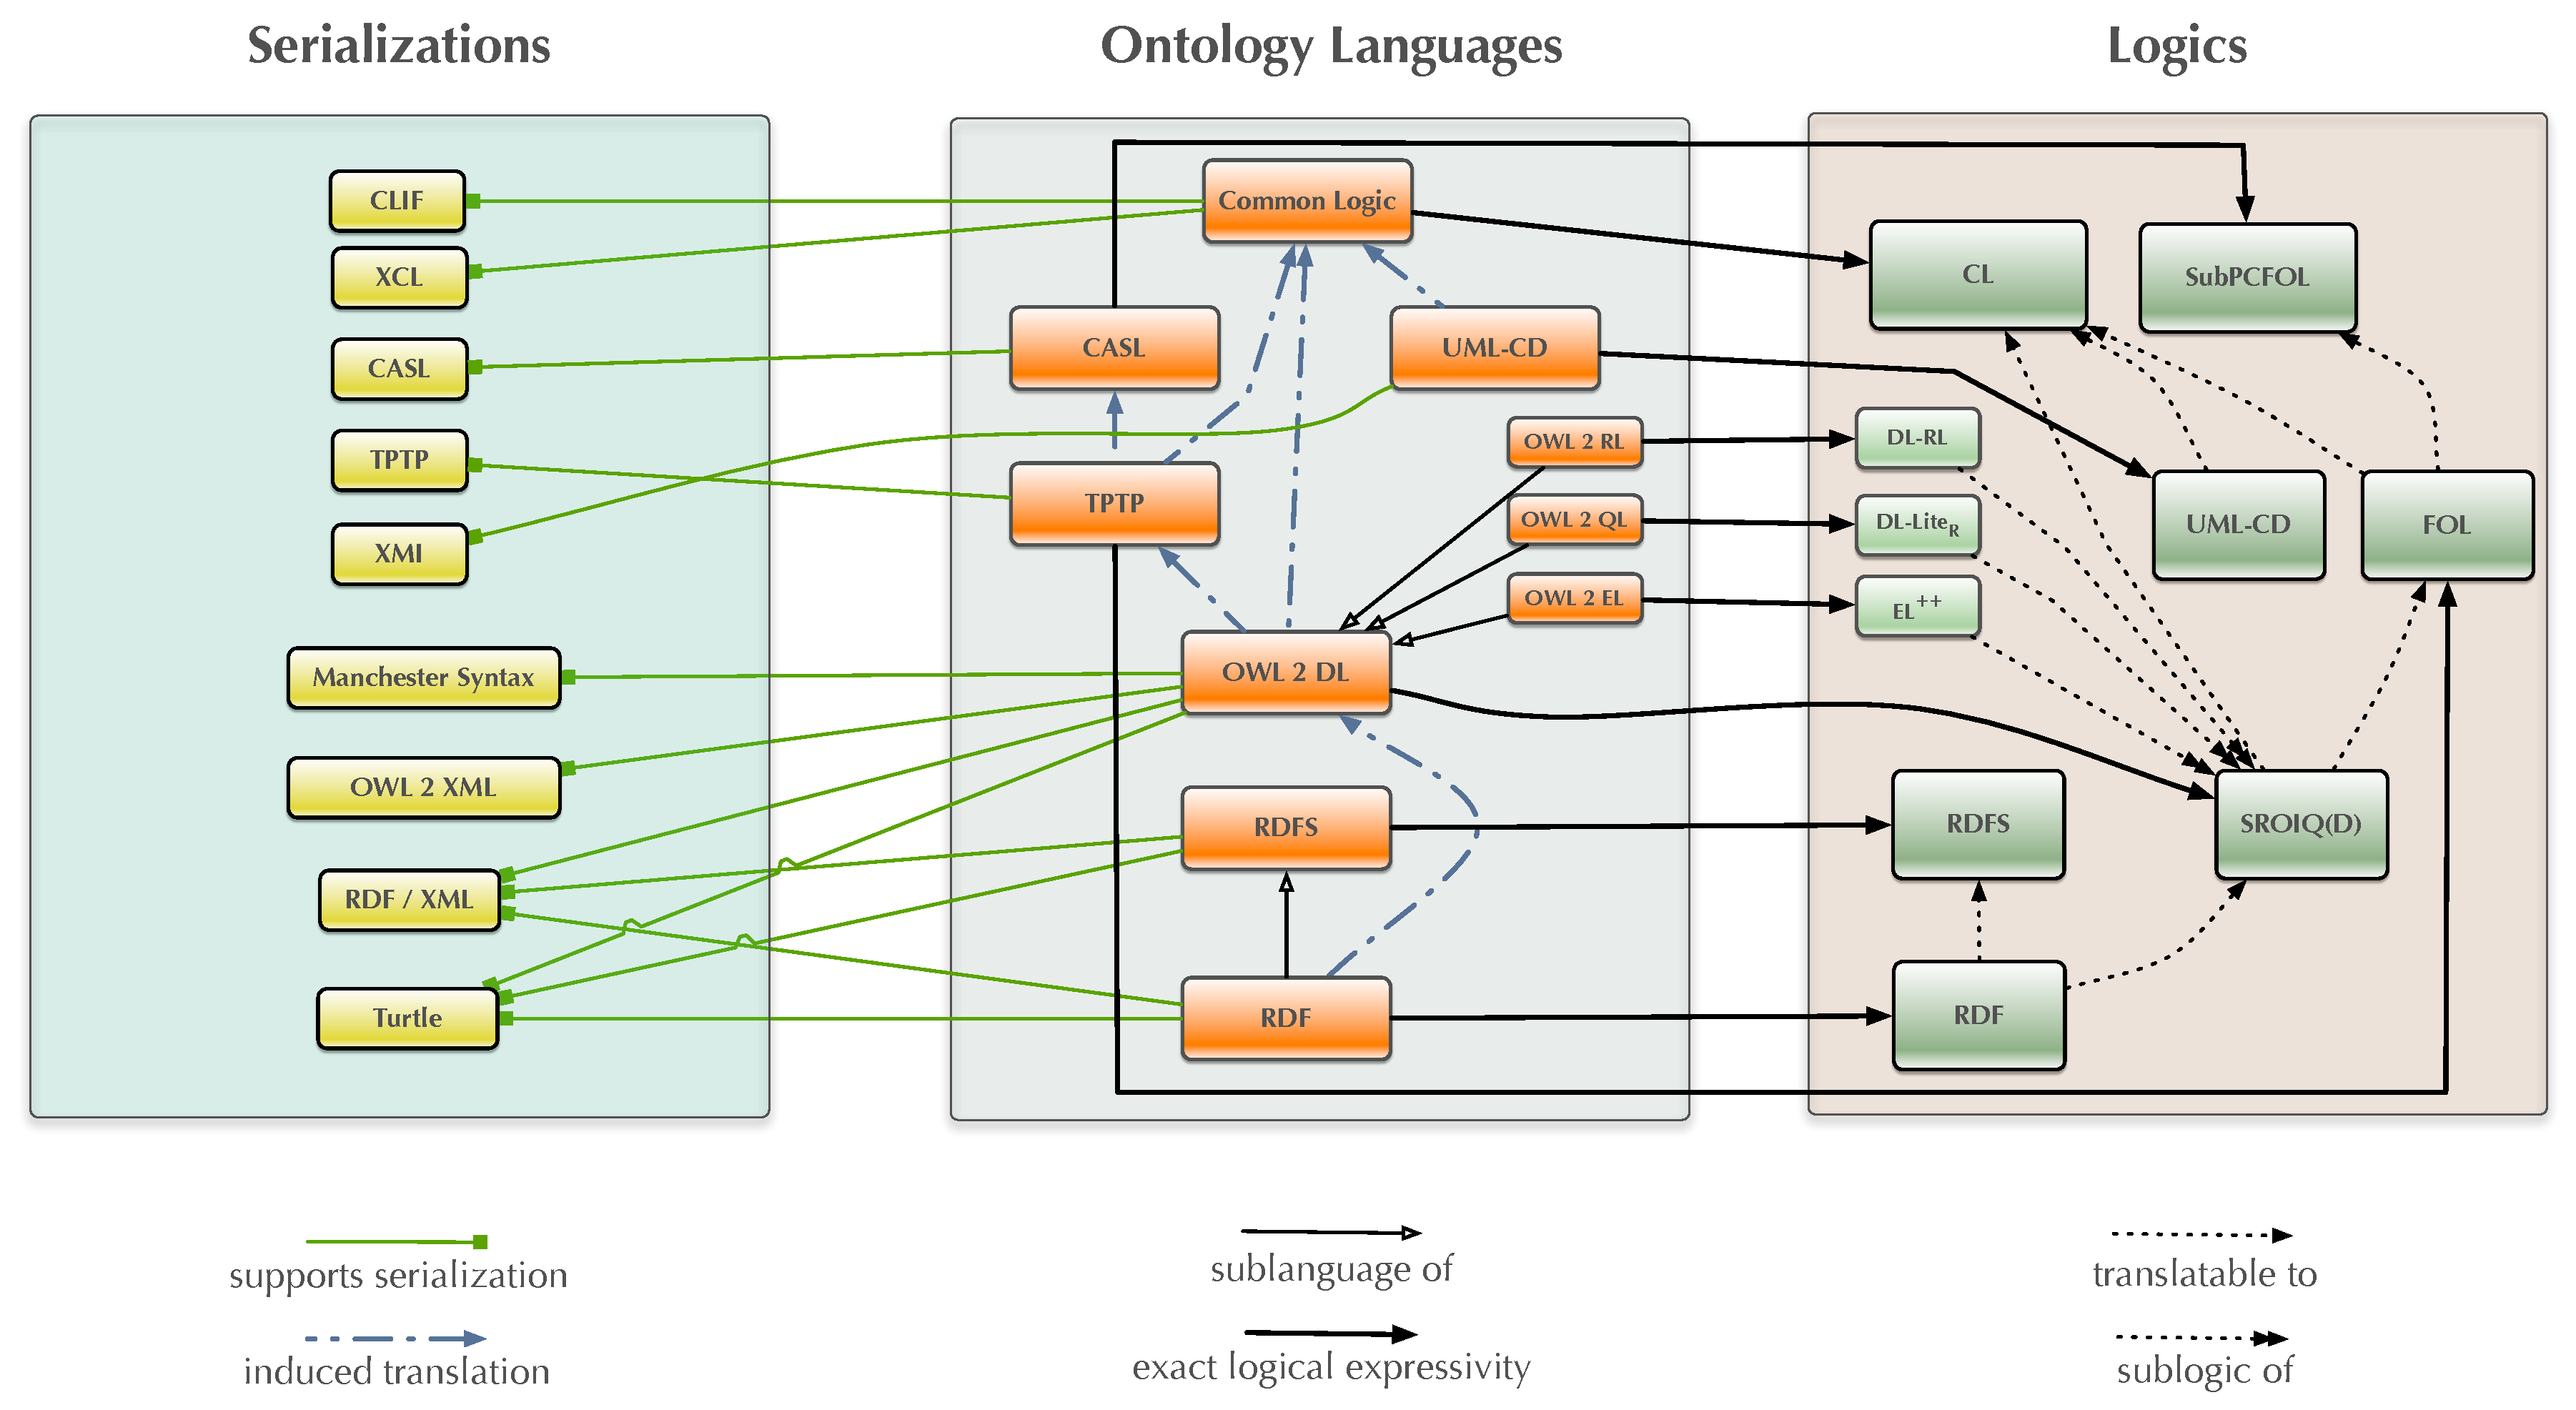
\includegraphics[width=\textwidth]{illustrations/DOL-ontograph-layers-OMG} 
  \caption{Subset of the OntoIOp registry, shown as an RDF graph}
\label{f:DOL-threelayers}
\end{sidewaysfigure}


\begin{figure}
  \centering
  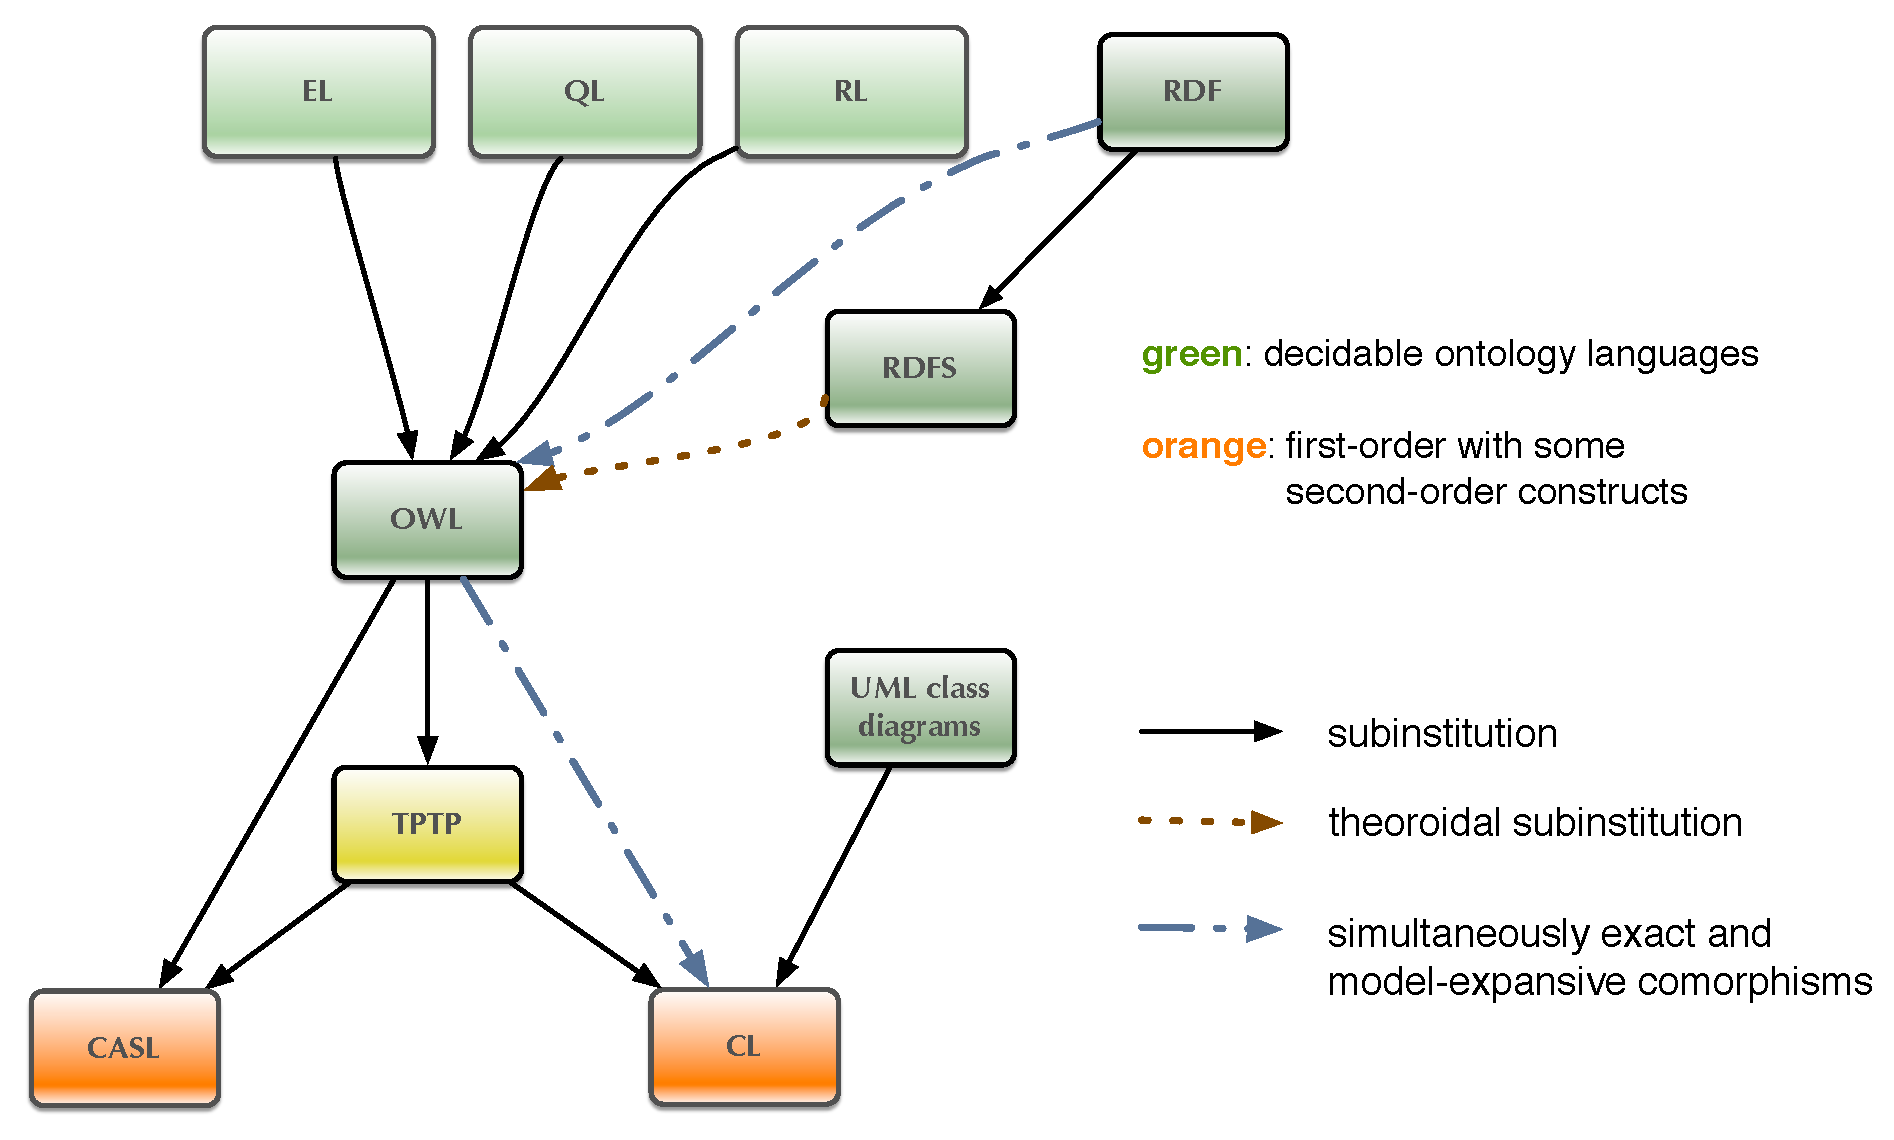
\includegraphics[width=\textwidth]{illustrations/ontograph-standards-new}
  \caption{Translations between conforming OMS languages}
  \label{fig:ontograph-standards}
\end{figure}

This annex provides a core heterogeneous environment that could be used as a basis for 
semantics of \DOL as defined in Sec.~\ref{c:semantics}.


%%%%%%%%%%%%%%%%%%%%%%%%%%%%%%%%%%%%%%%%%%%%%%%%%%%%%%%%%%%%%%%%%%%%%%%%%%%%%%%%%%%%%%%%%%%%%%%%%%%%%%%%%%%%%%%%%%%%%%%%%%%%%%%%%%
%%%%%%%%%%%%%%%%%%%%%%%%%%%%%%%%%%%%%%%%%%%%%%%%%%%%%%%%%%%%%%%%%%%%%%%%%%%%%%%%%%%%%%%%%%%%%%%%%%%%%%%%%%%%%%%%%%%%%%%%%%%%%%%%%%

\sclause{Languages}
 
The selected OMS languages are those whose conformance with \DOL is
established in the preceding annexes (OWL 2 DL in \aref{a:owl}, Common
Logic in \aref{a:cl}, RDFS in \aref{a:rdfs}, \CASL in \aref{a:casl}, UML
class models in \aref{a:uml-class} and TPTP in \aref{a:TPTP}).  The
logic graph is shown in \fref{fig:ontograph-standards}; the language
graph and supports relation in \fref{f:DOL-threelayers}.  Its nodes
refer to the following OMS languages and profiles:
\begin{itemize}
\item RDF \nref{RDF}
\item RDF Schema \nref{RDFS}
\item EL, QL, RL (all being profiles of OWL) \nref{OWL2-profiles}
\item OWL \nref{OWL2}
\item CL (Common Logic) \nref{CL}
\item UML class models \nref{UML}, version 2.5
\item \CASL \cite{CASL-RM} and its sublanguage classical first-order logic (FOL)
\item TPTP
\end{itemize}

%The list of chosen languages includes those ones required as mandatory
% ones in the RFP. Since these are only ontology and modeling
% languages, also a specification language is included, namely the
% Common Algebraic Specification Language (CASL).
The list of language translations, given below, comprises standard
translations from the literature~\cite{OntoGraph,MossakowskiEtAl14b}, as
well as further translations that are considered useful for logical
interoperability:
\begin{itemize}
  \item $\EL \to \OWL$ 
  \item $\QL \to \OWL$
  \item $\RL \to \OWL$
  \item $\RDF \to \RDFS$
  \item $\RDFS \to \OWL$
  \item $\OWL  \to \CASL.\FOL$
  \item $\CASL.\FOL \to \mathit{TPTP}$
  \item $\mathit{TPTP} \to \CASL.\FOL$
  \item $\CASL.\FOL \to \CL$
  \item $\CASL.\FOL \to \CASL$
  \item $\mathit{UML\textit{-}CD} \to \CL$.
\end{itemize}

The translations are specified in \cite{OntoGraph},\cite{MossakowskiEtAl14b}.
%~\todonote[author=Christoph Lange,type=todo]{Provide linear syntax here (as in the paper)}
Properties of translations have been introduced in section~\ref{s:foundations}.
All translations are marked as default translations. 


%%%%%%%%%%%%%%%%%%%%%%%%%%%%%%%%%%%%%%%%%%%%%%%%%%%%%%%%%%%%%%%%%%%%%%%%%%%%%%%%%%%%%%%%%%%%%%%%%%%%%%%%%%%%%%%%%%%%%%%%%%%%%%%%%%
%%%%%%%%%%%%%%%%%%%%%%%%%%%%%%%%%%%%%%%%%%%%%%%%%%%%%%%%%%%%%%%%%%%%%%%%%%%%%%%%%%%%%%%%%%%%%%%%%%%%%%%%%%%%%%%%%%%%%%%%%%%%%%%%%%

\sclause{Logics}

The logics giving the semantics of these languages are listed below:
\begin{itemize}
 \item \RDF and \RDFS, supported respectively by \RDF and \RDFS
 \item $\ELDL{+}{+}$, supported by the language \EL
 \item \DLLiteR, supported by \QL
 \item \RL, supported by \RL
 \item $\SROIQ(D)$, supported by $\OWL$
 \item \CL, supported by \CL
 \item $SubPCFOL^=_{ms}$, supported by \CASL
 \item \FOL, supported by $\CASL.FOL$ and $TPTP$
 \item $UML\mbox{-}CD$, supported by $UML\mbox{-}CD$.
\end{itemize}

The institution comorphisms between these logics are
\begin{itemize}
  \item $\ELDL{+}{+}$ $\to$ $\SROIQ(D)$ 
  \item \DLLiteR $\to$ $\SROIQ(D)$ 
  \item \RL $\to$ $\SROIQ(D)$ 
  \item $\RDF \to \RDFS$
  \item $\RDFS \to \SROIQ(D)$ 
  \item $\SROIQ(D)  \to \CASL.\FOL$
  \item $\FOL \to \CL$
  \item $\FOL \to SubPCFOL^=_{ms}$
  \item $UML\mbox{-}CD \to \CL$.
\end{itemize}

All of them are selected as default logic translations. There are no institution morphisms. The partial union operation between logics is given in the tables below, where
$\bot$ denotes undefinedness:


\begin{tabular}{| l | l | l | l | l | l |}
\hline
Union & $\ELDL{+}{+}$ & \DLLiteR & \RL & \RDF & \RDFS \\
\hline
$\ELDL{+}{+}$ & $\ELDL{+}{+}$ & $\SROIQ(D)$ & $\SROIQ(D)$ & $\SROIQ(D)$ & $\SROIQ(D)$ \\
\hline
\DLLiteR & $\SROIQ(D)$ & \DLLiteR & $\SROIQ(D)$ & $\SROIQ(D)$ & $\SROIQ(D)$ \\
\hline
\RL & $\SROIQ(D)$ &  $\SROIQ(D)$ & \RL & $\SROIQ(D)$ & $\SROIQ(D)$ \\
\hline
\RDF & $\SROIQ(D)$ &  $\SROIQ(D)$ &$\SROIQ(D)$ & \RDF & \RDFS \\
\hline
\RDFS & $\SROIQ(D)$ &  $\SROIQ(D)$ &$\SROIQ(D)$ & \RDFS & \RDFS \\
\hline
$\SROIQ(D)$& $\SROIQ(D)$ &  $\SROIQ(D)$ &$\SROIQ(D)$ & $\SROIQ(D)$ & $\SROIQ(D)$ \\
\hline
\FOL &  \FOL & \FOL & \FOL & \FOL & \FOL \\
\hline
$SubPCFOL^=_{ms}$ &  $SubPCFOL^=_{ms}$ & $SubPCFOL^=_{ms}$ & $SubPCFOL^=_{ms}$ & $SubPCFOL^=_{ms}$ & $SubPCFOL^=_{ms}$ \\
\hline
UML\mbox{-}CD & \CL & \CL & \CL & \CL & \CL \\
\hline
\CL &  \CL & \CL & \CL & \CL & \CL \\
\hline
\end{tabular}

\medskip

\begin{tabular}{| l | l | l | l | l | l |}
\hline
Union & $\SROIQ(D)$ & \FOL & $SubPCFOL^=_{ms}$ & UML\mbox{-}CD & \CL\\
\hline
$\ELDL{+}{+}$ & $\SROIQ(D)$ & \FOL & $SubPCFOL^=_{ms}$ & \CL & \CL\\
\hline
\DLLiteR & $\SROIQ(D)$ & \FOL & $SubPCFOL^=_{ms}$ & \CL& \CL\\
\hline
\RL  & $\SROIQ(D)$ & \FOL & $SubPCFOL^=_{ms}$ & \CL & \CL\\
\hline
\RDF  & $\SROIQ(D)$ & \FOL & $SubPCFOL^=_{ms}$ & \CL & \CL\\
\hline
\RDFS & $\SROIQ(D)$ & \FOL & $SubPCFOL^=_{ms}$ & \CL & \CL\\
\hline
$\SROIQ(D)$& $\SROIQ(D)$ & \FOL & $SubPCFOL^=_{ms}$ & \CL & \CL\\
\hline
\FOL &  \FOL & \FOL & $SubPCFOL^=_{ms}$ & \CL & \CL\\
\hline
$SubPCFOL^=_{ms}$ & $\SROIQ(D)$ & \FOL & $SubPCFOL^=_{ms}$ & $\bot$ & $\bot$\\
\hline
UML\mbox{-}CD & \CL & \CL & $\bot$ & UML\mbox{-}CD & \CL\\
\hline
\CL & \CL & \CL & $\bot$ & \CL & \CL\\
\hline
\end{tabular}


The other assumptions on the logics in the heterogeneous logical environment hold in
the expected way.\ednote{@Till: rephrase if need be. TM: I think it is OK, even if quite vague.}


%%%%%%%%%%%%%%%%%%%%%%%%%%%%%%%%%%%%%%%%%%%%%%%%%%%%%%%%%%%%%%%%%%%%%%%%%%%%%%%%%%%%%%%%%%%%%%%%%%%%%%%%%%%%%%%%%%%%%%%%%%%%%%%%%%
%%%%%%%%%%%%%%%%%%%%%%%%%%%%%%%%%%%%%%%%%%%%%%%%%%%%%%%%%%%%%%%%%%%%%%%%%%%%%%%%%%%%%%%%%%%%%%%%%%%%%%%%%%%%%%%%%%%%%%%%%%%%%%%%%%

\sclause{Serializations}

The following syntaxes are part of the heterogeneous logical environments:
\begin{itemize}
 \item Turtle, supported by $\OWL$, \EL, \QL, \RL , \RDF, \RDFS
 \item RDF-XML, supported by $\OWL$, \EL, \QL, \RL , \RDF, \RDFS
 \item OWL/XML, supported by $\OWL$, \EL, \QL, \RL 
 \item Manchester Syntax, supported by $\OWL$, \EL, \QL, \RL
  \item TPTP, supported by TPTP
  \item CASL, supported by \CASL
 \item XMI, supported by UML\mbox{-}CD
 \item XCL, supported by \CL
 \item CLIF, supported by \CL 
\end{itemize}


%%%%%%%%%%%%%%%%%%%%%%%%%%%%%%%%%%%%%%%%%%%%%%%%%%%%%%%%%%%%%%%%%%%%%%%%%%%%%%%%%%%%%%%%%%%%%%%%%%%%%%%%%%%%%%%%%%%%%%%%%%%%%%%%%%
%%%%%%%%%%%%%%%%%%%%%%%%%%%%%%%%%%%%%%%%%%%%%%%%%%%%%%%%%%%%%%%%%%%%%%%%%%%%%%%%%%%%%%%%%%%%%%%%%%%%%%%%%%%%%%%%%%%%%%%%%%%%%%%%%%

\sclause{Language and Logic Translations}

%%%%%%%%%%%%%%%%%%%%%%%%%%%%%%%%%%%%%%%%%%%%%%%%%%%%%%%%%%%%%%%%%%%%%%%%%%%%%%%%%%%%%%%%%%%%%%%%%%%%%%%%%%%%%%%%%%%%%%%%%%%%%%%%%%

\ssclause{\EL $\to$ $\OWL$ and $\ELDL{+}{+}$ $\to$ $\SROIQ(D)$}

\EL $\to$ $\OWL$ is the sublanguage inclusion obtained by the
syntactic restriction according to the definition of \EL, see
\nref{OWL2-profiles}. Since by definition, $\ELDL{+}{+}$
is a syntactic restriction of $\SROIQ(D)$, $\ELDL{+}{+}$ $\to$ $\SROIQ(D)$
is the corresponding sublogic inclusion.

%%%%%%%%%%%%%%%%%%%%%%%%%%%%%%%%%%%%%%%%%%%%%%%%%%%%%%%%%%%%%%%%%%%%%%%%%%%%%%%%%%%%%%%%%%%%%%%%%%%%%%%%%%%%%%%%%%%%%%%%%%%%%%%%%%

\ssclause{\QL $\to$ $\OWL$ and \DLLiteR $\to$ $\SROIQ(D)$}

\QL $\to$ $\OWL$ is the sublanguage inclusion obtained by the
syntactic restriction according to the definition of \QL, see
\nref{OWL2-profiles}. Since by definition, \DLLiteR
is a syntactic restriction of $\SROIQ(D)$, \DLLiteR $\to$ $\SROIQ(D)$
is the corresponding sublogic inclusion.

%%%%%%%%%%%%%%%%%%%%%%%%%%%%%%%%%%%%%%%%%%%%%%%%%%%%%%%%%%%%%%%%%%%%%%%%%%%%%%%%%%%%%%%%%%%%%%%%%%%%%%%%%%%%%%%%%%%%%%%%%%%%%%%%%%

\ssclause{\RL $\to$ $\OWL$ and $\RL$ $\to$ $\SROIQ(D)$}

\RL $\to$ $\OWL$ is the sublanguage inclusion obtained by the
syntactic restriction according to the definition of \RL, see
\nref{OWL2-profiles}. Since by definition, $\RL$
is a syntactic restriction of $\SROIQ(D)$, $\RL$ $\to$ $\SROIQ(D)$
is the corresponding sublogic inclusion.

%%%%%%%%%%%%%%%%%%%%%%%%%%%%%%%%%%%%%%%%%%%%%%%%%%%%%%%%%%%%%%%%%%%%%%%%%%%%%%%%%%%%%%%%%%%%%%%%%%%%%%%%%%%%%%%%%%%%%%%%%%%%%%%%%%

\ssclause{$\SimpleRDF \rightarrow \RDF$}

$\SimpleRDF \rightarrow \RDF$ is an obvious inclusion, except that
\SimpleRDF resources need to be renamed if they happen to have a predefined
meaning in \RDF. The model translation needs to forget the fixed parts
of \RDF realisations. Since this part can always reconstructed in a unique
way, the result is  an isomorphic model translation. 

%%%%%%%%%%%%%%%%%%%%%%%%%%%%%%%%%%%%%%%%%%%%%%%%%%%%%%%%%%%%%%%%%%%%%%%%%%%%%%%%%%%%%%%%%%%%%%%%%%%%%%%%%%%%%%%%%%%%%%%%%%%%%%%%%%

\ssclause{$\RDF \rightarrow \RDFS$}

This is entirely analogous to $\SimpleRDF \rightarrow \RDF$.

%%%%%%%%%%%%%%%%%%%%%%%%%%%%%%%%%%%%%%%%%%%%%%%%%%%%%%%%%%%%%%%%%%%%%%%%%%%%%%%%%%%%%%%%%%%%%%%%%%%%%%%%%%%%%%%%%%%%%%%%%%%%%%%%%%

\ssclause{$\SimpleRDF \rightarrow \SROIQ(D)$}

\todonote{This translation is not really useful. Consider the
  RDF-OWL-reduct construction instead.}


A $\SimpleRDF$ signature is translated to $\SROIQ(D)$ by providing a class
$P$ and three roles $sub$, $pred$ and $obj$ (these reify the extension
relation), and one individual per $\SimpleRDF$ resource. A $\SimpleRDF$ triple
$(s,p,o)$ is translated to the $\SROIQ(D)$ sentence
   $$\top \sqsubseteq \exists U. (\exists sub. \{s\} \sqcap \exists pred. \{p\} \sqcap  \exists obj. \{o\} ).$$
  From an $\SROIQ(D)$ realisation ${\cal I}$, obtain a \SimpleRDF realisation by inheriting the universe
  and the interpretation of individuals (then turned into resources).
  The interpretation $P^{\cal I}$ of $P$ gives $P_m$, and $EXT_m$ is obtained
  by de-reifying,
 i.e.\ $$EXT_{m}(x):=\{(y,z) \mid \exists u . (u,x)\in pred^{\cal I},
  (u,y)\in sub^{\cal I}, (u,z,)\in obj^{\cal I} \}.$$
  $\RDF \rightarrow \SROIQ(D)$ is defined similarly. The theory of \RDF built-ins 
  is (after translation to $\SROIQ(D)$) added to any signature translation.
  This ensures that the model translation can add the built-ins.
%\Til{What if the OWL model satisfies more triples than the built-ins?}

%%%%%%%%%%%%%%%%%%%%%%%%%%%%%%%%%%%%%%%%%%%%%%%%%%%%%%%%%%%%%%%%%%%%%%%%%%%%%%%%%%%%%%%%%%%%%%%%%%%%%%%%%%%%%%%%%%%%%%%%%%%%%%%%%%

\ssclause{$\OWL \rightarrow FOL$}

%%%%%%%%%%%%%%%%%%%%%%%%%%%%%%%%%%%%%%%%%%%%%%%%%%%%%%%%%%%%%%%%%%%%%%%%%%%

\sssclause{Translation of signatures}

 $\Phi((\Concepts, \Roles, \Individuals)) =  (F, P)$ with
\begin{itemize}
	\item function symbols: $F = \{a^{(1)} \vert a \in \Individuals\}$
	\item predicate symbols $P = \{A^{(1)} \vert A \in \category{C} \} \cup \{ R^{(2)} \vert R \in \category{R}\}$
\end{itemize}

%%%%%%%%%%%%%%%%%%%%%%%%%%%%%%%%%%%%%%%%%%%%%%%%%%%%%%%%%%%%%%%%%%%%%%%%%%%

\sssclause{Translation of sentences}

Concepts are translated as follows:
\begin{itemize}
 \item $\alpha_x(A) = A(x)$
 \item $\alpha_x(\top) = \mathit{true}$
 \item $\alpha_x(\bot) = \mathit{false}$
 \item $\alpha_x(\lnot C) = \lnot \alpha_x (C)$
 \item $\alpha_x(C \sqcap D) = \alpha_x(C) \land \alpha_x(D)$
 \item $\alpha_x(C \sqcup D) = \alpha_x(C) \lor \alpha_x(D)$ 
 \item $\alpha_x(\exists R.C) = \exists y . (R(x,y) \land \alpha_y(C))$
 \item $\alpha_x(\exists U.C) = \exists y . \alpha_y(C)$
 \item $\alpha_x(\forall R.C) = \forall y . (R(x,y) \rightarrow \alpha_y(C))$
 \item $\alpha_x(\forall U.C) = \forall y . \alpha_y(C)$
 \item $\alpha_x(\exists R.\text{Self}) = R(x,x)$
 \item $\alpha_x(\leq n R. C) = \forall y_1,\ldots,y_{n+1} .  \bigwedge_{i=1,\ldots,n+1}(R(x,y_i) \land \alpha_{y_i}(C)) \rightarrow\bigvee_{1\leq i<j\leq n+1}y_i = y_j$
 \item $\alpha_x(\geq n R. C) = \exists y_1,\ldots,y_n . \bigwedge_{i=1,\ldots,n}(R(x,y_i) \land \alpha_{y_i}(C)) \wedge \bigwedge_{1\leq i<j\leq n}y_i\not= y_j $
 \item $\alpha_x(\{a_1, \ldots a_n \}) = (x=a_1\vee \ldots \vee x=a_n)$
\end{itemize}

For inverse roles $R^-$, $R^-(x,y)$ has to be replaced by $R(y,x)$, e.g.
 $$\alpha_x(\exists R^-.C) = \exists y . (R(y,x) \land \alpha_y(C))$$
This rule also applies below.


Sentences are translated as follows:

\begin{itemize}
 \item $\alpha_\Sigma (C \sqsubseteq D) = \forall x.\, (\alpha_x(C) \rightarrow \alpha_x(D))$
 \item $\alpha_\Sigma (a:C) = \alpha_x(C)[x\mapsto a]$\footnote{$t[x\mapsto a]$ means ``in $t$, replace $x$ by $a$''.}
 \item $\alpha_\Sigma (R(a,b)) = R(a,b)$
 \item $\alpha_\Sigma (R \sqsubseteq S) = \forall x, y. R(x,y) \rightarrow S(x,y) $
 \item $\alpha_\Sigma (R_1; \ldots; R_n \sqsubseteq R) =$\\
$ \forall x,y . (\exists z_1,\ldots, z_{n-1} . R_1(x,z_1) \wedge R_2(z_1,z_2) \wedge \ldots \wedge R_n(z_{n-1},y)) \rightarrow R(x,y) $
 \item $\alpha_\Sigma (\text{Dis}(R_1,R_2)) = \neg\exists x,y . R_1(x,y)\wedge R_2(x,y)$	
 \item $\alpha_\Sigma (\text{Ref}(R)) = \forall x. R(x,x)$
 \item $\alpha_\Sigma (\text{Irr}(R)) = \forall x. \neg R(x,x)$
 \item $\alpha_\Sigma (\text{Asy}(R)) = \forall x,y . R(x,y) \rightarrow \neg R(y,x)$
 \item $\alpha_\Sigma (\text{Tra}(R)) = \forall x,y,z . R(x,y) \wedge R(y,z) \rightarrow R(x,z)$
\end{itemize}

%%%%%%%%%%%%%%%%%%%%%%%%%%%%%%%%%%%%%%%%%%%%%%%%%%%%%%%%%%%%%%%%%%%%%%%%%%%

\sssclause{Translation of realisations}

\begin{itemize}
	\item For $M' \in \Models^{FOL}(\Phi \Sigma)$ define $\I=\beta_\Sigma(M') := (\Delta, \cdot^\I)$
	with $\Delta = |M'|$ and $A^\I = M'_A, a^\I = M'_a, R^\I = M'_R$.
\end{itemize}

	\begin{proposition}
$C^\I = \left\{m \in \Delta \lvert M' + \{x \mapsto m \} \models \alpha_x (C) \right\}$
	\end{proposition}
	
	\begin{proof} By induction over the structure of $C$.
\begin{itemize}
	\item $A^\I = M'_A = \left \{m \in \Delta \vert M' + \{x \mapsto m \} \models A(x)  \right\}$
	\item $(\lnot C)^\I = \Delta \setminus C^\I =^{I.H.} \Delta \setminus \{m \in \Delta \lvert M' + \{x \mapsto m\} \models \alpha_x(C)\} = \{m \in \Delta  \vert M' + \{x \mapsto m\} \models \lnot \alpha_x(C)\}$
\end{itemize}
	\end{proof}

        The other cases are similar.

	 The satisfaction condition now follows easily.

%%%%%%%%%%%%%%%%%%%%%%%%%%%%%%%%%%%%%%%%%%%%%%%%%%%%%%%%%%%%%%%%%%%%%%%%%%%%%%%%%%%%%%%%%%%%%%%%%%%%%%%%%%%%%%%%%%%%%%%%%%%%%%%%%%

\ssclause{$FOL \rightarrow \CL$}

This comorphism  maps classical first-order logic (FOL) to Common Logic.

%It maps constants to
%  discourse names and function and predicate symbols to non-discourse
%  names, with a straightforward sentence and model translation;

A FOL signature is translated to \Clogic.Fol by turning all constants
into discourse names, and all other function symbols and all predicate
symbols into non-discourse names. A FOL sentence is translated
to \Clogic.Fol by a straightforward recursion, the base being translations
of predications:
$$\alpha_\Sigma(P(t_1,\ldots,t_n)) = (P\ \alpha_\Sigma(t_1)\ \ldots\ \alpha_\Sigma(t_n))$$
Within terms, function applications are translated similarly:
$$\alpha_\Sigma(f(t_1,\ldots,t_n)) = (f\ \alpha_\Sigma(t_1)\ \ldots\ \alpha_\Sigma(t_n))$$
A \Clogic.Fol realisation is translated to a FOL realisation 
by using the universe of
discourse as FOL universe. The interpretation of constants is
directly given by the interpretation of the corresponding names
in \Clogic.Fol. The interpretation of a predicate symbol $P$ is given
by using $rel^M(int^M(P))$ and restricting to the arity of $P$;
similarly for function symbols (using $fun^M$). Both the satisfaction condition
and model-expansiveness of the comorphism are straightforward.

%%%%%%%%%%%%%%%%%%%%%%%%%%%%%%%%%%%%%%%%%%%%%%%%%%%%%%%%%%%%%%%%%%%%%%%%%%%%%%%%%%%%%%%%%%%%%%%%%%%%%%%%%%%%%%%%%%%%%%%%%%%%%%%%%%

\ssclause{$\OWL \rightarrow \CL$}

This comorphism is the composition of the comorphisms described in the previous
two sections.

%%%%%%%%%%%%%%%%%%%%%%%%%%%%%%%%%%%%%%%%%%%%%%%%%%%%%%%%%%%%%%%%%%%%%%%%%%%%%%%%%%%%%%%%%%%%%%%%%%%%%%%%%%%%%%%%%%%%%%%%%%%%%%%%%%
\ssclause{UML class models $\to \CL$}


This translation has been described in annex~\ref{a:uml-class}. 
Translation of signatures is detailed in section~\ref{a:UML-CD-models},
translation of sentences in section~\ref{a:UML-CD-sat}.
Realisations are translated identically.

%%%%%%%%%%%%%%%%%%%%%%%%%%%%%%%%%%%%%%%%%%%%%%%%%%%%%%%%%%%%%%%%%%%%%%%%%%%%%%%%%%%%%%%%%%%%%%%%%%%%%%%%%%%%%%%%%%%%%%%%%%%%%%%%%%

\ssclause{$FOL \to \CASL$}
This is an obvious sublogic.

%%%%%%%%%%%%%%%%%%%%%%%%%%%%%%%%%%%%%%%%%%%%%%%%%%%%%%%%%%%%%%%%%%%%%%%%%%%%%%%%%%%%%%%%%%%%%%%%%%%%%%%%%%%%%%%%%%%%%%%%%%%%%%%%%%

\ssclause{UML class model to \OWL}
Let $\Sigma = ((C, {\leq_C}), P, O, A, M)$ be a \emph{class/data type net} representing a UML 
class model as described in annex~\ref{a:uml-class}. This net can be translated to OWL2 using the approach described in \cite{zedlitz2012uml}.
The ontology is extended by translating parts of this net and its multiplicity constraints $\mathit{Mult}(\Sigma)$:
\begin{itemize}
\item For each class $c \in C$ with superclasses $c_1,c_2,\ldots,c_n \in C$ (i.e.\ $c \leq_C c_i$ for $i=1,\ldots,n$):
\begin{lstlisting}[language=owl2Manchester]
	Class: c
		SubClassOf: c1
		...
		SubClassOf: cn
\end{lstlisting}
\item For each attribute declaration $c.p:c'$ in $P$
\begin{lstlisting}[language=owl2Manchester]
	ObjectProperty: p
		Domain: c
		Range: c'
\end{lstlisting}

\item For each attribute multiplicity $n\ \mathsf{\leq}\ c.p:\tau[c']$ in $\mathit{Mult}(\Sigma)$ extend the description of class $c$ by:
\begin{lstlisting}[language=owl2Manchester]
	SubClassOf: p min n c'
\end{lstlisting}

\item For each attribute multiplicity $ c.p:\tau[c'] \ \mathsf{\leq}\ n$  in $\mathit{Mult}(\Sigma)$ extend the description of class $c$ by:
\begin{lstlisting}[language=owl2Manchester]
	SubClassOf: p max n c'
\end{lstlisting}

\item For each unidirectional binary association declaration $a(p_1:\tau_1[c_1],p_2:\tau_2[c_2])$ in $A$:
\begin{lstlisting}[language=owl2Manchester]
	ObjectProperty: p
		Domain: c1
		Range: c2
\end{lstlisting}
\item For each bidirectional binary association declaration $a(p_1:\tau_1[c_1],p_2:\tau_2[c_2])$ in $A$:
\begin{lstlisting}[language=owl2Manchester]
	ObjectProperty: p1
		Domain: c
		Range: c'

	ObjectProperty: p2
		Characteristics: InverseFunctional
		Domain: c
		Range: c'
		InverseOf: p1
\end{lstlisting}
\item For each binary association $n \leq a(p_1:\tau_1[c_1],p_2:\tau_2[c_2]).p_i$, with $i \neq j\in\{1,2\}$ in $\mathit{Mult}(\Sigma)$ extend the description of class $c_j$ by:
\begin{lstlisting}[language=owl2Manchester]
	SubClassOf: pi min n ci
\end{lstlisting}
\item For each binary association $a(p_1:\tau_1[c_1],p_2:\tau_2[c_2]).p_i \leq n$, with $i \neq j\in\{1,2\}$  in $\mathit{Mult}(\Sigma)$ extend the description of class $c_j$ by:
\begin{lstlisting}[language=owl2Manchester]
	SubClassOf: pi max n ci
\end{lstlisting}
\item For each composition declaration $m(\mathsf{Set}[c_1], \composition p_2 :
\tau_2[c_2])$ in $M$:
\begin{lstlisting}[language=owl2Manchester]
	ObjectProperty: p
		Characteristics:
			Functional, 
			Irreflexive
		Domain: c1
		Range: c2
\end{lstlisting}
\item For each binary association $n \leq a(p_1:\tau_1[c_1], \composition p_2:\tau_2[c_2]).p_i$, with $i \neq j\in\{1,2\}$  in $\mathit{Mult}(\Sigma)$  extend the description of class $c_j$ by:
\begin{lstlisting}[language=owl2Manchester]
	SubClassOf: pi min n ci
\end{lstlisting}
\item For each binary association $a(p_1:\tau_1[c_1], \composition p_2:\tau_2[c_2]).p_i \leq n$, with $i \neq j\in\{1,2\}$  in $\mathit{Mult}(\Sigma)$ extend the description of class $c_j$ by:
\begin{lstlisting}[language=owl2Manchester]
	SubClassOf: pi max n ci
\end{lstlisting}
\end{itemize}
 
%%%%%%%%%%%%%%%%%%%%%%%%%%%%%%%%%%%%%%%%%%%%%%%%%%%%%%%%%%%%%%%%%%%%%%%%%%%%%%%%%%%%%%%%%%%%%%%%%%%%%%%%%%%%%%%%%%%%%%%%%%%%%%%%%%
%%%%%%%%%%%%%%%%%%%%%%%%%%%%%%%%%%%%%%%%%%%%%%%%%%%%%%%%%%%%%%%%%%%%%%%%%%%%%%%%%%%%%%%%%%%%%%%%%%%%%%%%%%%%%%%%%%%%%%%%%%%%%%%%%%

\sclause{Formal Representation of Language and Logic Translations}
\label{sec:repr-trans}

A formal representation of language and logic translations still needs
to be developed. For the syntax aspects of these translations, QVT
could be a useful option. However, it would have added value to choose
a representation of translations that allows  their correctness
to be proven easily. Such a representation would have to interact
with suitable representations of languages and logics in a 
logical framework. See \cite{CodescuEtAl2011d} for some work
in this direction.

%%%%%%%%%%%%%%%%%%%%%%%%%%%%%%%%%%%%%%%%%%%%%%%%%%%%%%%%%%%%%%%%%%%%%%%%%%%%%%%%%%%%%%%%%%%%%%%%%%%%%%%%%%%%%%%%%%%%%%%%%%%%%%%%%%
%%%%%%%%%%%%%%%%%%%%%%%%%%%%%%%%%%%%%%%%%%%%%%%%%%%%%%%%%%%%%%%%%%%%%%%%%%%%%%%%%%%%%%%%%%%%%%%%%%%%%%%%%%%%%%%%%%%%%%%%%%%%%%%%%%
%%%%%%%%%%%%%%%%%%%%%%%%%%%%%%%%%%%%%%%%%%%%%%%%%%%%%%%%%%%%%%%%%%%%%%%%%%%%%%%%%%%%%%%%%%%%%%%%%%%%%%%%%%%%%%%%%%%%%%%%%%%%%%%%%%

\cleardoublepage
\infannex{Extended Logic Graph}\label{a:ext-graph}

\begin{figure}
  \centering
  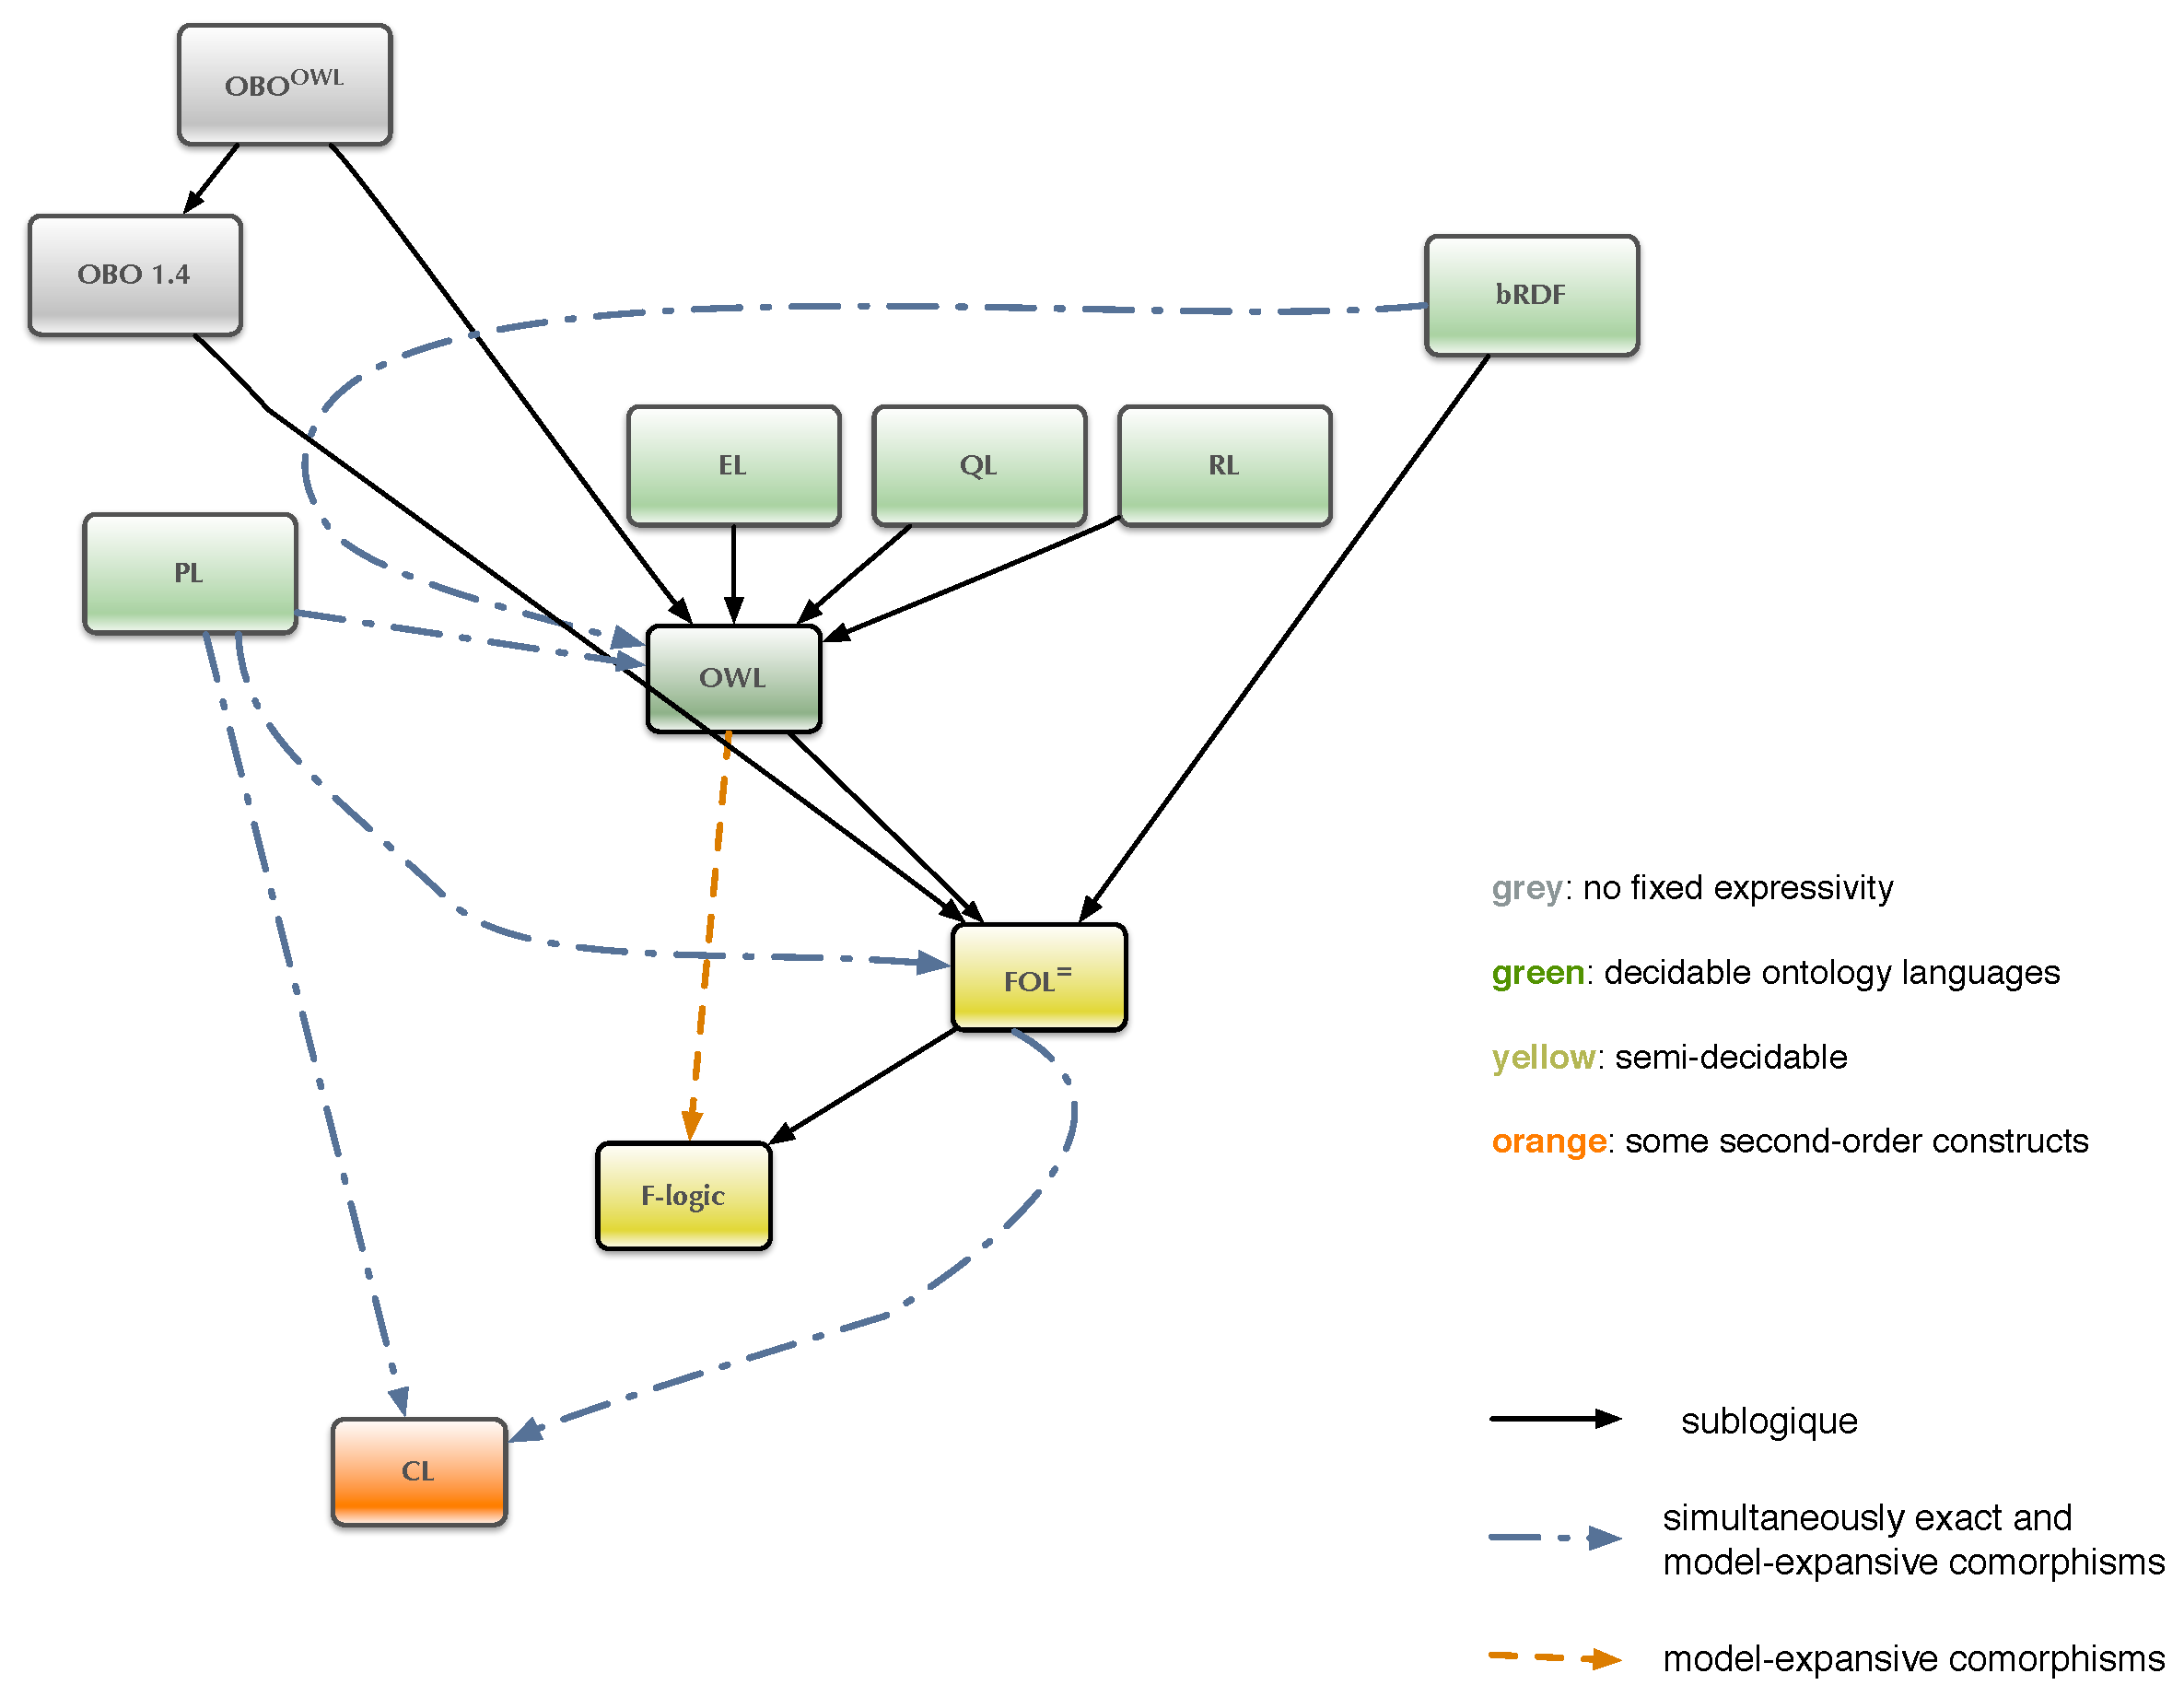
\includegraphics[width=\textwidth]{illustrations/pre-reduced-ontograph}
  \caption{Translations between conforming OMS languages (extended)}
  \label{fig:pre-ontograph}
\end{figure}
This annex extends the graph of logics and translations given in
\aref{a:graph} by a list of OMS languages  whose inclusion in
the registry is planned.  The graph is shown in
\fref{fig:pre-ontograph}.  Its nodes are included in the following
list of OMS languages and profiles (in addition to those
mentioned in \aref{a:graph}):
\begin{itemize}
\item PL (propositional logic)
\item SimpleRDF (RDF triples without a reserved vocabulary)
\item OBO\textsuperscript{OWL} and OBO1.4
\item RIF \nref{RIF} (Rule Interchange Format)
\item EER (Enhanced Entity-Relationship Models) % see Talheim Thalheim, B. (2009). Extended entity relationship model. In L. Liu and M. T. Ozsu, editors, En- cyclopedia of Database Systems, volume 1, pages 1083-1091. Springer.
\item Datalog
\item ORM (object role modeling)
\item the meta model of schema.org
\item different model types of the UML (Unified Modeling Language), with possibly different logics according to different
UML semantics
\item SKOS (Simple Knowledge Organization System; \nref{SKOS})
\item FOL\textsuperscript{=} (untyped first-order logic, as used for the
TPTP format)
\item F-logic
%\item CASL (Common Algebraic Specification Language)
\end{itemize}

The actual translations are specified in \cite{OntoGraph}.

%~\todonote[author=Christoph Lange,type=todo]{Provide linear syntax here (as in the paper). TM: what do you mean by this?}

%%%%%%%%%%%%%%%%%%%%%%%%%%%%%%%%%%%%%%%%%%%%%%%%%%%%%%%%%%%%%%%%%%%%%%%%%%%%%%%%%%%%%%%%%%%%%%%%%%%%%%%%%%%%%%%%%%%%%%%%%%%%%%%%%%
%%%%%%%%%%%%%%%%%%%%%%%%%%%%%%%%%%%%%%%%%%%%%%%%%%%%%%%%%%%%%%%%%%%%%%%%%%%%%%%%%%%%%%%%%%%%%%%%%%%%%%%%%%%%%%%%%%%%%%%%%%%%%%%%%%
%%%%%%%%%%%%%%%%%%%%%%%%%%%%%%%%%%%%%%%%%%%%%%%%%%%%%%%%%%%%%%%%%%%%%%%%%%%%%%%%%%%%%%%%%%%%%%%%%%%%%%%%%%%%%%%%%%%%%%%%%%%%%%%%%%

\cleardoublepage
\infannex{\DOL Abstract Syntax in EBNF}
\label{a:EBNF}
\sclause{General}

The following subclauses specify the abstract syntax of \DOL in EBNF. Note that it deviates from the EBNF specification in
 \nref{EBNF} in favor of a more concise
EBNF syntax. More precisely, \nref{EBNF} requires commas between the (non-)terminals of a right-hand side, which are omitted 
for the sake of better readability. Also, the separator \syntax{=}
between left and right hand-side of a rule is replaced with \syntax{::=}, and 
 the notation \syntax{N+} is used 
for one or more repetitions of \syntax{N}.
%Note that ISO EBNF lacks an operator for ``at least one repetition''.  This \IS therefore adopts the following convention: Whenever some sequence \syntax{S} is repeated at least once, we give it a non-terminal identifier of its own (\syntax{RepeatedS = S \{ S \} ;}), or group it as in \syntax{LongerExpression = Foo Bar ( S \{ S \} ) ;}.

Note that the EBNF abstract syntax is constructor-based.
E.g. \syntax{translation} is a constructor that can be used to build
more complex OMS from smaller OMS (and in general, the constructors
can be used to form syntax trees). By contrast, the MOF-based abstract
syntax in clause~\ref{c:abstract-syntax} is selector-based, i.e.\ it
features selectors that, given a complex OMS, extract the simpler OMS
that are its building blocks. While the metaclasses of the MOF
metamodel largely match the non-terminal symbols of the EBNF abstract
syntax, there is no such direct match between selectors and
constructors.

The non-terminals of the EBNF abstract syntax largely match those of
the concrete syntax given in clause~\ref{c:abstract-syntax}. Some
non-terminals of the concrete syntax have been omitted in the abstract 
syntax, because they serve merely syntactical purposes and do not
contribute to a useful syntax tree. Otherwise, the productions of
the concrete syntax match those of the abstract syntax, but the
abstract syntax constructors are replaced with specific strings
(possibly interspersed at different positions) expressing the
concrete syntax.


% Corresponds to image mof/libraries.png and mof/prefixes.png

%%%%%%%%%%%%%%%%%%%%%%%%%%%%%%%%%%%%%%%%%%%%%%%%%%%%%%%%%%%%%%%%%%%%%%%%%%%%%%%%%%%%%%%%%%%%%%%%%%%%%%%%%%%%%%%%%%%%%%%%%%%%%%%%%%
%%%%%%%%%%%%%%%%%%%%%%%%%%%%%%%%%%%%%%%%%%%%%%%%%%%%%%%%%%%%%%%%%%%%%%%%%%%%%%%%%%%%%%%%%%%%%%%%%%%%%%%%%%%%%%%%%%%%%%%%%%%%%%%%%%


\sclause{Documents}\label{e:libraries}
\begin{lstlisting}[language=ebnf,escapeinside={@@}]  % abstract syntax

Document           ::= DOLLibrary | NativeDocument
DOLLibrary         ::= library [PrefixMap] LibraryName Qualification
                               LibraryItem*
NativeDocument     ::= @$<$@language specific@$>$@ 
LibraryItem        ::= LibraryImport | Definition | Qualification
Definition         ::= OMSDefinition
                     | NetworkDefinition
                     | MappingDefinition
                     | QueryRelatedDefinition
LibraryImport      ::= lib-import LibraryName
Qualification      ::= LanguageQualification
                     | LogicQualification
                     | SyntaxQualification
LanguageQualification ::= lang-select LanguageRef
LogicQualification ::= logic-select LogicRef
SyntaxQualification ::= syntax-select SyntaxRef
LanguageRef        ::= IRI
LogicRef           ::= IRI
SyntaxRef          ::= IRI
LibraryName        ::= IRI
PrefixMap          ::= prefix-map PrefixBinding*
Prefix             ::= String
Separators         ::= separators LibraryOMSSeparator OMSSymbolSeparator
LibraryOMSSeparator ::= String
OMSSymbolSeparator ::= String
\end{lstlisting}

%% ~\todonote[type=fyi,author=Christoph Lange]{Things changed from HetCASL:\textLF
%%   • logic-select now mandatory (no default logic) and tree-scoped MC: what does this mean? To make Hets-lib conform with this, we should have .het files equivalent to .dol files with logic selected to be CASL\textLF
%%   • download-items (encourage linked data best practices instead)\textLF
%%   • item-name-map (to be replaced by namespaces??)\textLF
%%   • lib-version (to be replaced by metadata annotations, \eg OMV)\textLF
%%   • indirect-mapping (will always use full IRIs, and abbreviate them by syntactic namespaces)}

%%%%%%%%%%%%%%%%%%%%%%%%%%%%%%%%%%%%%%%%%%%%%%%%%%%%%%%%%%%%%%%%%%%%%%%%%%%%%%%%%%%%%%%%%%%%%%%%%%%%%%%%%%%%%%%%%%%%%%%%%%%%%%%%%%
%%%%%%%%%%%%%%%%%%%%%%%%%%%%%%%%%%%%%%%%%%%%%%%%%%%%%%%%%%%%%%%%%%%%%%%%%%%%%%%%%%%%%%%%%%%%%%%%%%%%%%%%%%%%%%%%%%%%%%%%%%%%%%%%%%

% Corresponds to image mof/networks.png
\sclause{OMS Networks}\label{a:networks}
\begin{lstlisting}[language=ebnf,escapeinside={@@}]  % abstract syntax

NetworkDefinition ::= network-definition NetworkName
                                         [ConservativityStrength] Network
NetworkName         ::= IRI
Network             ::= network NetworkElement* ExcludedElement*
NetworkElement      ::= network-element [Id] IRI
ExcludedElement     ::= PathReference | ExcludedElementRef
PathReference       ::= path IRI IRI
ExcludedElementRef  ::= IRI
\end{lstlisting}


%%%%%%%%%%%%%%%%%%%%%%%%%%%%%%%%%%%%%%%%%%%%%%%%%%%%%%%%%%%%%%%%%%%%%%%%%%%%%%%%%%%%%%%%%%%%%%%%%%%%%%%%%%%%%%%%%%%%%%%%%%%%%%%%%%
%%%%%%%%%%%%%%%%%%%%%%%%%%%%%%%%%%%%%%%%%%%%%%%%%%%%%%%%%%%%%%%%%%%%%%%%%%%%%%%%%%%%%%%%%%%%%%%%%%%%%%%%%%%%%%%%%%%%%%%%%%%%%%%%%%

\sclause{OMS}

% Corresponds to image mof/oms.png and mof/basic_oms.png
\begin{lstlisting}[language=ebnf,escapeinside={@@}]  % abstract syntax

BasicOMS           ::= @$<$@ language specific @$>$@ 
OMS                ::= ExtendingOMS
                     | ClosureOMS
                     | TranslationOMS
                     | ReductionOMS
                     | ExtractionOMS
                     | ApproximationOMS
                     | FilteringOMS
                     | UnionOMS
                     | ExtensionOMS
                     | QualifiedOMS
                     | CombinationOMS
                     | ApplicationOMS
ClosureOMS         ::= closure-symbols OMS Closure
TranslationOMS     ::= translation OMS OMSTranslation
ReductionOMS       ::= reduction OMS Reduction
ExtractionOMS      ::= module-extract OMS Extraction
ApproximationOMS   ::= approximation OMS Approximation
FilteringOMS       ::= filtering OMS Filtering
UnionOMS           ::= union OMS [ConservativityStrength] OMS
ExtensionOMS       ::= extension OMS Extension
QualifiedOMS       ::= qualified-oms Qualification Qualification* OMS
CombinationOMS     ::= combination Network
ApplicationOMS     ::= application OMS SubstName
OMSDefinition      ::= oms-definition OMSName [ConservativityStrength] OMS
ConservativityStrength ::= consequence-conservative
                     | model-conservative
                     | not-consequence-conservative
                     | not-model-conservative
                     | implied
                     | monomorphic
                     | weak-definitional
                     | definitional
OMSName            ::= IRI
SubstName          ::= IRI
\end{lstlisting}

% Corresponds to image mof/extension&closure.png
\begin{lstlisting}[language=ebnf,escapeinside={@@}]  % abstract syntax
ClosableOMS        ::= BasicOMS | OMSReference
OMSReference       ::= oms-reference OMSRef [ImportName]
Extension          ::= extension [ConservativityStrength]
                                 [ExtensionName] ExtendingOMS
ExtendingOMS       ::= ClosableOMS | RelativeClosureOMS
RelativeClosureOMS ::= relative-closure ClosureType ClosableOMS
Closure            ::= ClosureType CircClosure CircVars
ClosureType        ::= minimize | maximize | free | cofree
CircClosure        ::= Symbol Symbol*
CircVars           ::= Symbol*
ExtensionName      ::= IRI
ImportName         ::= IRI
OMSRef             ::= IRI
\end{lstlisting}
%% \ednote{Alternatively, we could use one type of \syntax{InterfaceSignature}
%% only, and instead use different constructors for \syntax{Extraction}
%% and \syntax{Approximation}. This would be a bit more verbose, but a bit
%% more coherent with position of non-terminals in the concrete syntax.}

%%%%%%%%%%%%%%%%%%%%%%%%%%%%%%%%%%%%%%%%%%%%%%%%%%%%%%%%%%%%%%%%%%%%%%%%%%%%%%%%%%%%%%%%%%%%%%%%%%%%%%%%%%%%%%%%%%%%%%%%%%%%%%%%%%
%%%%%%%%%%%%%%%%%%%%%%%%%%%%%%%%%%%%%%%%%%%%%%%%%%%%%%%%%%%%%%%%%%%%%%%%%%%%%%%%%%%%%%%%%%%%%%%%%%%%%%%%%%%%%%%%%%%%%%%%%%%%%%%%%%

% Corresponds to image mof/translation&reduction.png
\begin{lstlisting}[language=ebnf,escapeinside={@@}]  % abstract syntax
OMSTranslation     ::= translate OMSLanguageTranslation* [SymbolMap]
Reduction          ::= reduction RemovalKind OMSLanguageTranslation*
                                 [SymbolList]
SymbolList         ::= Symbol Symbol*
SymbolMap          ::= symbol-map GeneralSymbolMapItem
                                  GeneralSymbolMapItem*
Extraction         ::= extraction RemovalKind InterfaceSignature
Approximation      ::= approx RemovalKind [InterfaceSignature] [LogicRef]
Filtering          ::= filter RemovalKind BasicOMSOrSymbolList
BasicOMSOrSymbolList ::= BasicOMS | SymbolList
InterfaceSignature ::= SymbolList
SymbolMapItem      ::= symbol-map-item Symbol Symbol
GeneralSymbolMapItem ::= Symbol | SymbolMapItem
OMSLanguageTranslation ::= NamedTranslation | DefaultTranslation
NamedTranslation   ::= named-trans OMSLanguageTranslationRef
DefaultTranslation ::= default-trans LanguageRef
RemovalKind        ::= keep | remove
OMSLanguageTranslationRef ::= IRI
Symbol             ::= IRI
\end{lstlisting}


%%%%%%%%%%%%%%%%%%%%%%%%%%%%%%%%%%%%%%%%%%%%%%%%%%%%%%%%%%%%%%%%%%%%%%%%%%%%%%%%%%%%%%%%%%%%%%%%%%%%%%%%%%%%%%%%%%%%%%%%%%%%%%%%%%
%%%%%%%%%%%%%%%%%%%%%%%%%%%%%%%%%%%%%%%%%%%%%%%%%%%%%%%%%%%%%%%%%%%%%%%%%%%%%%%%%%%%%%%%%%%%%%%%%%%%%%%%%%%%%%%%%%%%%%%%%%%%%%%%%%

\sclause{OMS Mappings}

% Corresponds to image mof/interpretation&refinement.png
\begin{lstlisting}[language=ebnf,escapeinside={<>},mathescape]  % abstract syntax
InterpretationDefinition ::= interpretation-definition
                                                       InterpretationName
                                                       [ConservativityStrength]
                                                       InterpretationType
                                                       OMSLanguageTranslation*
                                                       [SymbolMap]
RefinementDefinition ::= refinement InterpretationName Refinement
InterpretationName ::= IRI
InterpretationType ::= interpretation-type OMS OMS
Refinement         ::= RefinementOMS
                     | RefinementNetwork
                     | SimpleOMSRefinement
                     | SimpleNetworkRefinement
RefinementOMS      ::= refinement-oms OMS
RefinementNetwork  ::= refinement-network Network
SimpleOMSRefinement ::= simple-oms-ref Refinement OMSRefinementMap Refinement
SimpleNetworkRefinement ::= simple-network-ref Refinement
                                               NetworkRefinementMap Refinement
OMSRefinementMap   ::= oms-refmap [OMSLanguageTranslation] [SymbolMap]
NetworkRefinementMap ::= network-refmap Refinement*
\end{lstlisting}

% Corresponds to image mof/entailment&equivalence.png
\begin{lstlisting}[language=ebnf,escapeinside={<>},mathescape]  % abstract syntax
MappingDefinition  ::= InterpretationDefinition
                     | RefinementDefinition
                     | EntailmentDefinition
                     | EquivalenceDefinition
                     | ConservativeExtensionDefinition
                     | AlignmentDefinition
EntailmentDefinition ::= entailment EntailmentName EntailmentType
OMSOMSEntailment   ::= oms-oms-entailment OMS OMS
NetworkOMSEntailment ::= network-oms-entailment Network OMSName OMS
NetworkNetworkEntailment ::= network-network-entailment Network Network
EntailmentType     ::= OMSOMSEntailment
                     | NetworkOMSEntailment
                     | NetworkNetworkEntailment
EntailmentName     ::= IRI
EquivalenceDefinition ::= equivalence-definition
                                                 EquivalenceName
                                                 EquivalenceType
EquivalenceName    ::= IRI
EquivalenceType    ::= OMSEquivalence | NetworkEquivalence
OMSEquivalence     ::= oms-equivalence OMS OMS [OMS]
NetworkEquivalence ::= network-equivalence Network Network [Network]
\end{lstlisting}

% Corresponds to image mof/alignment.png
\begin{lstlisting}[language=ebnf,escapeinside={@@},mathescape]  % abstract syntax
AlignmentDefinition ::= alignment-definition AlignmentName
                              [AlignmentCardinality] [AlignmentCardinality]
                              AlignmentType Correspondence*
                              [AlignmentSemantics]<\footnote{%
                        Note that this grammar uses ``type'' as in
                        ``the type of a function'', whereas the Alignment API
                        \cite{AlignmentAPI} uses ``type''  for\:  the
                        totality/injectivity of the relation/function.  For the
                        latter, this grammar uses ``cardinality''.}>
AlignmentName      ::= IRI
AlignmentCardinality ::= injective-and-total
                     | injective
                     | total
                     | neither-injective-nor-total
AlignmentType      ::= alignment-type OMS OMS
AlignmentSemantics ::= single-domain
                     | global-domain
                     | contextualized-domain
Correspondence     ::= CorrespondenceBlock
                     | SingleCorrespondence
                     | DefaultCorrespondence
DefaultCorrespondence ::= default-correspondence
CorrespondenceBlock ::= correspondence-block [Relation]
                                             [Confidence] Correspondence
                                             Correspondence*
SingleCorrespondence ::= correspondence Symbol [Relation]
                                        [Confidence] GeneralizedTerm
                                        [CorrespondenceID]
CorrespondenceID   ::= IRI
GeneralizedTerm    ::= Symbol
Symbol             ::= IRI
Relation           ::= RelationReference | StandardRelation
StandardRelation   ::= StandardRelationValues
StandardRelationValues ::= subsumes
                     | is-subsumed
                     | equivalent
                     | incompatible
                     | has-instance
                     | instance-of
                     | default-relation
RelationReference  ::= relation-ref IRI
Confidence         ::= Double
Double             ::= @$<$ a number $\in [0,1]$ $>$@ 
\end{lstlisting}

% Corresponds to image mof/modules.png
\begin{lstlisting}[language=ebnf,escapeinside={@@},mathescape]  % abstract syntax
ConservativeExtensionDefinition ::= cons-ext-definition ConservativeExtensionName
                                          [ConservativityStrength] ConservativeExtensionType
                                          InterfaceSignature
ConservativeExtensionName         ::= IRI
ConservativeExtensionType         ::= cons-ext-type OMS OMS
\end{lstlisting}

%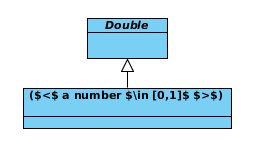
\includegraphics[scale=0.6]{mof/dia/dia5.png}


%%%%%%%%%%%%%%%%%%%%%%%%%%%%%%%%%%%%%%%%%%%%%%%%%%%%%%%%%%%%%%%%%%%%%%%%%%%%%%%%%%%%%%%%%%%%%%%%%%%%%%%%%%%%%%%%%%%%%%%%%%%%%%%%%%
%%%%%%%%%%%%%%%%%%%%%%%%%%%%%%%%%%%%%%%%%%%%%%%%%%%%%%%%%%%%%%%%%%%%%%%%%%%%%%%%%%%%%%%%%%%%%%%%%%%%%%%%%%%%%%%%%%%%%%%%%%%%%%%%%%

\sclause{IRIs and Prefixes}
% Corresponds to image mof/prefixes.png
\begin{lstlisting}[language=ebnf,escapeinside={@@}]  % abstract syntax
PrefixBinding      ::= prefix-binding Prefix FullIRI [Separators]
IRI    ::= FullIRI | CurieIRI@\footnote{Specified below in \cref{c:curies}.}@
CurieIRI ::= curie CURIE
FullIRI ::= @$<$ as defined by the IRI production in \nref{IRI} $>$@ 
CURIE  ::= String
\end{lstlisting}

%%%%%%%%%%%%%%%%%%%%%%%%%%%%%%%%%%%%%%%%%%%%%%%%%%%%%%%%%%%%%%%%%%%%%%%%%%%%%%%%%%%%%%%%%%%%%%%%%%%%%%%%%%%%%%%%%%%%%%%%%%%%%%%%%%
%%%%%%%%%%%%%%%%%%%%%%%%%%%%%%%%%%%%%%%%%%%%%%%%%%%%%%%%%%%%%%%%%%%%%%%%%%%%%%%%%%%%%%%%%%%%%%%%%%%%%%%%%%%%%%%%%%%%%%%%%%%%%%%%%%
%%%%%%%%%%%%%%%%%%%%%%%%%%%%%%%%%%%%%%%%%%%%%%%%%%%%%%%%%%%%%%%%%%%%%%%%%%%%%%%%%%%%%%%%%%%%%%%%%%%%%%%%%%%%%%%%%%%%%%%%%%%%%%%%%%

\cleardoublepage
\infannex{Extension of \DOL with Queries}\label{a:queries}
\sclause{General}
This annex describes the syntax of queries. A semantics still needs to
be developed.  \DOL's metaclass \syntax{LibraryItem} is extended with a
new subclass \syntax{QueryRelatedDefinition} for definitions related to
queries.

%%%%%%%%%%%%%%%%%%%%%%%%%%%%%%%%%%%%%%%%%%%%%%%%%%%%%%%%%%%%%%%%%%%%%%%%%%%%%%%%%%%%%%%%%%%%%%%%%%%%%%%%%%%%%%%%%%%%%%%%%%%%%%%%%%
%%%%%%%%%%%%%%%%%%%%%%%%%%%%%%%%%%%%%%%%%%%%%%%%%%%%%%%%%%%%%%%%%%%%%%%%%%%%%%%%%%%%%%%%%%%%%%%%%%%%%%%%%%%%%%%%%%%%%%%%%%%%%%%%%%

\sclause{Terms and Definitions}
\begin{definitions}
  \termdefinition{query language}{\termref{OMS language} specifically dedicated to queries\index{query}.}
\begin{example}
SPARQL, Prolog
\end{example}
\begin{note}
There are also general purpose OMS languages, which can express both \termref{OMS} and queries.
\end{note}



\termdefinition{query}{\termref{sentence} containing query variables\index{query variable}
   that can be instantiated by a \termref{substitution}.}


\termdefinition{query variable}{\termref{symbol} that will be used in a \termref{query} and a
\termref{substitution}.}
  \begin{note}
   From an abstract point of view, query variables are just symbols; 
   they are used in a way
   that they will be substituted using a substitution.
   Many OMS languages have special notations for (query) variables.
  \end{note}
  \begin{note}
   Usually, query variables are the free variables of a sentence; there
   can be other (bound) variables.
  \end{note}
  \begin{note}
  If there are no variables in an OMS language, constants can be used as query
  variables.
  \end{note}


\termdefinition{substitution}{\termref{OMS mapping} that maps query variables\index{query variable} of one \termref{OMS} to complex terms\index{term} of another OMS.}



\termdefinition{answer substitution}{\termref{substitution} that, when applied to
   a given \termref{query}, turns the latter into a logical consequence of a
   given \termref{OMS}.}
\end{definitions}  


%%%%%%%%%%%%%%%%%%%%%%%%%%%%%%%%%%%%%%%%%%%%%%%%%%%%%%%%%%%%%%%%%%%%%%%%%%%%%%%%%%%%%%%%%%%%%%%%%%%%%%%%%%%%%%%%%%%%%%%%%%%%%%%%%%
%%%%%%%%%%%%%%%%%%%%%%%%%%%%%%%%%%%%%%%%%%%%%%%%%%%%%%%%%%%%%%%%%%%%%%%%%%%%%%%%%%%%%%%%%%%%%%%%%%%%%%%%%%%%%%%%%%%%%%%%%%%%%%%%%%

\sclause{MOF Abstract Syntax}
Queries are a means to extract information from an OMS.  \DOL's \syntax{QueryDefinition}s cover 
``select''-type queries that deliver an answer substitution for the query variables. (Answer) 
substitutions can be stored separately, using a \syntax{Substitution\-Definition}. A
\syntax{ResultDefinition} expresses that certain answer substitutions are
the result of a query. Optionally, a result can be expressed to be
complete, meaning that it comprises all answer substitutions to the query.
 Note that by default, OMS are employed with an open world semantics,
but using minimizations, (part of) OMS can be equipped with a closed
world semantics. The corresponding extension of the DOL metamodel is shown
in Fig.~\ref{fig:queries}.

\begin{figure}
    \centering
      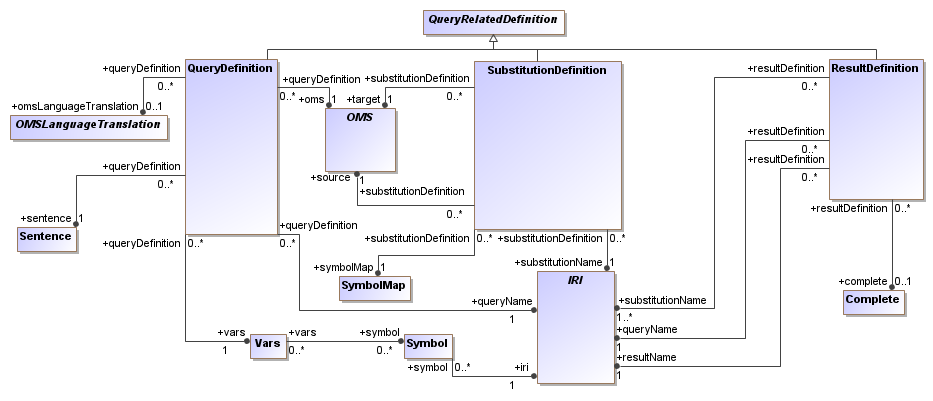
\includegraphics[scale=0.5]{mof/queries.png}
     \caption{Extension of DOL metamodel with queries}
    \label{fig:queries} 
\end{figure}


%%%%%%%%%%%%%%%%%%%%%%%%%%%%%%%%%%%%%%%%%%%%%%%%%%%%%%%%%%%%%%%%%%%%%%%%%%%%%%%%%%%%%%%%%%%%%%%%%%%%%%%%%%%%%%%%%%%%%%%%%%%%%%%%%%
%%%%%%%%%%%%%%%%%%%%%%%%%%%%%%%%%%%%%%%%%%%%%%%%%%%%%%%%%%%%%%%%%%%%%%%%%%%%%%%%%%%%%%%%%%%%%%%%%%%%%%%%%%%%%%%%%%%%%%%%%%%%%%%%%%

\sclause{EBNF Concrete Syntax}

% Corresponds to image mof/queries.png
\begin{lstlisting}[language=ebnf,escapeinside={@@},mathescape]

Term               ::= @$<$@ an expression specific to an OMS language @$>$@ 
GeneralizedTerm    ::= Term | Symbol
QueryRelatedDefinition ::= QueryDefinition
                     | SubstitutionDefinition
                     | ResultDefinition
QueryDefinition    ::= 'query' QueryName '=' 'select' Vars 'where'
                       Sentence 'in' GroupOMS
                       ['along' OMSLanguageTranslation] 'end'
SubstitutionDefinition ::= 'substitution' SubstitutionName ':'
                           GroupOMS 'to' GroupOMS '=' SymbolMap
                           'end'
ResultDefinition   ::= 'result' ResultName '=' SubstitutionName
                       ( ',' SubstitutionName )* 'for' QueryName
                       ['%complete'] 'end'
OMS                ::= @$\dots$@ | OMS 'with' SubstitutionName 
QueryName          ::= IRI
SubstitutionName   ::= IRI
ResultName         ::= IRI
Vars               ::= Symbol ( ',' Symbol )*
\end{lstlisting}

%%%%%%%%%%%%%%%%%%%%%%%%%%%%%%%%%%%%%%%%%%%%%%%%%%%%%%%%%%%%%%%%%%%%%%%%%%%%%%%%%%%%%%%%%%%%%%%%%%%%%%%%%%%%%%%%%%%%%%%%%%%%%%%%%%
%%%%%%%%%%%%%%%%%%%%%%%%%%%%%%%%%%%%%%%%%%%%%%%%%%%%%%%%%%%%%%%%%%%%%%%%%%%%%%%%%%%%%%%%%%%%%%%%%%%%%%%%%%%%%%%%%%%%%%%%%%%%%%%%%%

\sclause{EBNF Abstract Syntax}


\begin{lstlisting}[language=ebnf,escapeinside={@@},mathescape]  % abstract syntax

QueryRelatedDefinition ::= QueryDefinition
                     | SubstitutionDefinition
                     | ResultDefinition
QueryDefinition    ::= select-query-definition
                                               QueryName Vars Sentence OMS
                                               [OMSLanguageTranslation]
SubstitutionDefinition ::= substitution-definition
                                                   SubstitutionName OMS OMS
                                                   SymbolMap
ResultDefinition   ::= result-definition ResultName
                                         SubstitutionName SubstitutionName*
                                         QueryName [Complete]
Sentence           ::= @$<$@ an expression specific to an OMS language @$>$@ 
OMS                ::= @$\ldots$@ | application  OMS  SubstitutionName 
QueryName          ::= IRI
SubstitutionName   ::= IRI
ResultName         ::= IRI
Vars               ::= Symbol*
Complete           ::= complete
\end{lstlisting}

%%%%%%%%%%%%%%%%%%%%%%%%%%%%%%%%%%%%%%%%%%%%%%%%%%%%%%%%%%%%%%%%%%%%%%%%%%%%%%%%%%%%%%%%%%%%%%%%%%%%%%%%%%%%%%%%%%%%%%%%%%%%%%%%%%
%%%%%%%%%%%%%%%%%%%%%%%%%%%%%%%%%%%%%%%%%%%%%%%%%%%%%%%%%%%%%%%%%%%%%%%%%%%%%%%%%%%%%%%%%%%%%%%%%%%%%%%%%%%%%%%%%%%%%%%%%%%%%%%%%%

\sclause{Semantics of Queries}\label{s:sem-queries}

While queries are very important from a practical point of view, their
semantics so far has been developed only for individual institutions.
In \cite{MossakowskiEtAl15a}, three options for an
institution-independent semantics of queries and derived signature
morphisms (which can map symbols to terms) are discussed. Currently,
it is not clear which one would be the best choice. It is expected
that after some experience with \DOL, a choice will crystallize. This
means that in the current version, the semantics of queries is
elided, and left for a later version of \DOL.

% \semdom{sem(\syntax{QueryRelatedDefinition})}
%
%%%%%%%%%%%%%%%%%%%%%%
% \semdom{sem(\syntax{QueryDefinition})}
%%%%%%%%%%%%%%%%%%%%%
% \semdom{sem(\syntax{SubstitutionDefinition})}
%%%%%%%%%%%%%%%%%%%%%%
% \semdom{sem(\syntax{ResultDefinition})}
%%%%%%%%%%%%%%%%%%%%%%%%
%
%%Application
%\semdom{sem^T(\syntax{application OMS Substitutionname})}
%\semdom{sem^M(\syntax{application OMS Substitutionname})}
%
%
%\semdom{sem(\Gamma,\Sigma,\syntax{Term}) = t}

%$$sem(\Gamma, \Sigma, \syntax{Term}) = t$$
%\noindent where $t$ is a $\Sigma$-term and the analysis is done in a logic-specific way.\ednote{This should be added to the heterogeneous logical env. We here need derived siganture morphisms.}

%%%%%%%%%%%%%%%%%%%%%%%%%%%%%%%%%%%%%%%%%%%%%%%%%%%%%%%%%%%%%%%%%%%%%%%%%%%%%%%%%%%%%%%%%%%%%%%%%%%%%%%%%%%%%%%%%%%%%%%%%%%%%%%%%%
%%%%%%%%%%%%%%%%%%%%%%%%%%%%%%%%%%%%%%%%%%%%%%%%%%%%%%%%%%%%%%%%%%%%%%%%%%%%%%%%%%%%%%%%%%%%%%%%%%%%%%%%%%%%%%%%%%%%%%%%%%%%%%%%%%
%%%%%%%%%%%%%%%%%%%%%%%%%%%%%%%%%%%%%%%%%%%%%%%%%%%%%%%%%%%%%%%%%%%%%%%%%%%%%%%%%%%%%%%%%%%%%%%%%%%%%%%%%%%%%%%%%%%%%%%%%%%%%%%%%%

\cleardoublepage
\infannex{Example Uses of all \DOL Constructs}\label{a:uses}
\sclause{General}
This annex provides example uses of \DOL constructs.  Jointly with
\cref{c:goal}, which  contains \DOL examples for the
usage scenarios, all \DOL constructs (although not necessarily all
variants of each construct) are covered.  The examples follow the \DOL
Text Serialization (\cref{c:abstract-syntax}). The following table
provides an overview of which \DOL language constructs have been 
covered where.



%\CLnote[type=q-aut]{Should we have another column here that refers to the \emph{abstract} syntax?}%
\begin{tabular}{|l|l|}\hline
\multicolumn{2}{|c|}{\textbf{Top-level declarations in \DOL libraries}}\\\hline
\textbf{Top-level declaration} & \textbf{Examples} \\\hline
library \ldots & all examples\\\hline
import IRI & Mereology\\\hline
language IRI  & Alignments, Publications \\\hline
logic IRI  & Alignments, Mereology \\\hline
serialization IRI  & Alignments, Mereology \\\hline
PrefixMap  & Mereology \\\hline
oms IRI = OMS end  &  Alignments, Mereology \\\hline
oms IRI = \%consistent OMS end  & PropositionalExamples, Mereology \\\hline
oms IRI = \%inconsistent OMS end  & PropositionalExamples \\\hline
oms IRI = \%mono OMS end  & section~\ref{spec-2} \\\hline
oms IRI = \%def OMS end  & PropositionalExamples \\\hline
network IRI = IRI, \ldots, IRI & Alignments \\\hline
%network IRI = IRI, \ldots, IRI & \\
%\qquad excluding IRI, \ldots, IRI -> IRI & \\\hline
interpretation IRI : OMS to OMS = SymbolMap  & Mereology \\\hline
interpretation IRI : OMS to OMS = \%cons SymbolMap  &  Engine\\\hline
interpretation IRI : OMS to OMS = translation IRI  & Mereology \\\hline
refinement IRI = OMS refined via SymbolMap to OMS & section~\ref{spec-2} \\\hline
refinement IRI = OMS refined via translation IRI to OMS & section~\ref{model-2} \\\hline
refinement IRI = IRI refined to IRI & section~\ref{spec-2} \\\hline
refinement IRI = Network refined to Network & section~\ref{model-1} \\\hline
entailment IRI = OMS entails OMS & PropositionalExamples \\\hline
entailment IRI = OMSName in Network entails OMS & section~\ref{model-1}\\\hline
entailment IRI = Network entails Network & section~\ref{model-1}\\\hline
equivalence IRI : OMS \lessthan-\greaterthan\ OMS = OMS end  &  Algebra \\\hline
%equivalence IRI : Network \lessthan-\greaterthan\ Network = Network end  &  \\\hline
cons-ext IRI : OMS of OMS for Symbols  & section~\ref{onto-3} \\\hline
%module IRI \%ccons : OMS of OMS for Symbols  &  \\\hline
%alignment IRI : OMS to OMS end  &  \\\hline
%alignment IRI 1 : OMS to OMS end  &  \\\hline
%alignment IRI ? : OMS to OMS end  &  \\\hline
%alignment IRI + : OMS to OMS end  &  \\\hline
%alignment IRI * : OMS to OMS end  &  \\\hline
alignment IRI : OMS to OMS = Correspondences  & Alignments \\\hline
alignment IRI : OMS to OMS = Correspondences & \\
\qquad assuming SingleDomain & \cite{OM2014} \\\hline
alignment IRI : OMS to OMS = Correspondences & \\
\qquad assuming GlobalDomain & \cite{OM2014} \\\hline
alignment IRI : OMS to OMS = Correspondences & \\
\qquad assuming ContextualizedDomain & \cite{OM2014} \\\hline
query IRI = select ars where Sen in OMS & MyQuery\\\hline
substitution IRI : OMS to OMS = SymbolMap & MyQuery\\\hline
result IRI = IRIs for IRI & MyQuery\\\hline
\end{tabular}

\begin{tabular}{|l|l|}\hline
\multicolumn{2}{|c|}{\textbf{OMS}}\\\hline
\textbf{OMS notation} & \textbf{Examples} \\\hline
BasicOMS  & Alignments, Mereology \\\hline
IRI  & Alignments, Mereology \\\hline
%IRI \%( IRI )\%  &  \\\hline
minimize \{ OMS \}  & BlocksWithCircumscription \\\hline
OMS minimize Symbols var Symbols  & BlocksWithCircumscription \\\hline
OMS maximize Symbols var Symbols  & BlocksWithCircumscription \\\hline
%OMS then minimize \{ OMS \} &  \\\hline
%OMS then maximize \{ OMS \} &  \\\hline
free \{ OMS \} & Datatypes \\\hline
cofree \{ OMS \} & Datatypes \\\hline
OMS with SymbolMap  & Alignments,  section~\ref{spec-2} \\\hline
OMS with translation IRI  & Mereology \\\hline
%OMS with translation IRI : IRI $\to$ IRI  &  \\\hline
%OMS with translation IRI $\to$ IRI  &  \\\hline
%OMS with translation $\to$ IRI  &  \\\hline
OMS hide SymbolList  &  Algebra \\\hline
OMS reveal Symbols  & Datatypes \\\hline
%OMS reveal Symbol |-> Symbol ...  &  \\\hline
OMS hide along IRI  & section~\ref{model-1}, MetricSpaces \\\hline
%OMS hide along IRI : IRI $\to$ IRI  &  \\\hline
%OMS hide along IRI $\to$ IRI  &  \\\hline
%OMS hide along $\to$ IRI  &  \\\hline
OMS extract Symbols  & section~\ref{onto-3} \\\hline
OMS remove Symbols  & All\_kinds\_of\_group\_specifications \\\hline
OMS forget Symbols  & All\_kinds\_of\_group\_specifications \\\hline
%OMS forget Symbols keep Logic  &  \\\hline
OMS keep Symbols  & All\_kinds\_of\_group\_specifications \\\hline
%OMS keep Symbols keep Logic &  \\\hline
OMS select BasicOMS  & All\_kinds\_of\_group\_specifications  \\\hline
OMS reject BasicOMS  & All\_kinds\_of\_group\_specifications \\\hline
OMS and OMS   & Engine \\\hline
OMS then OMS  & Mereology \\\hline
OMS then \%ccons OMS  &  \cite{DBLP:conf/ijcai/LutzWW07} \\\hline
%OMS then \%ccons \%( IRI )\% OMS  &  \\\hline
OMS then \%mcons OMS  & Propositional \\\hline
OMS then \%notccons OMS  & \cite{DBLP:conf/ijcai/LutzWW07} \\\hline
OMS then \%notmcons OMS  & \cite{DBLP:conf/ijcai/LutzWW07} \\\hline
OMS then \%mono OMS  & Sorting \\\hline
%OMS then \%wdef OMS  &  \\\hline
OMS then \%def OMS  & Persons \\\hline
OMS then \%implied OMS  &  BlocksWithCircumscription \\\hline
logic IRI : OMS  &  all examples\\\hline
language IRI : OMS  &  Mereology\\\hline
serialization IRI : OMS  & Mereology \\\hline
combine NetworkElements  & Alignments, Publications \\\hline
%combine NetworkElements excluding IRIs  &  \\\hline
\end{tabular}

%%%%%%%%%%%%%%%%%%%%%%%%%%%%%%%%%%%%%%%%%%%%%%%%%%%%%%%%%%%%%%%%%%%%%%%%%%%%%%%%%%%%%%%%%%%%%%%%%%%%%%%%%%%%%%%%%%%%%%%%%%%%%%%%%%
%%%%%%%%%%%%%%%%%%%%%%%%%%%%%%%%%%%%%%%%%%%%%%%%%%%%%%%%%%%%%%%%%%%%%%%%%%%%%%%%%%%%%%%%%%%%%%%%%%%%%%%%%%%%%%%%%%%%%%%%%%%%%%%%%%

\sclause{Simple Examples in Propositional Logic}\label{ex:prop}
\begin{lstlisting}[basicstyle=\ttfamily,language=dolText,alsolanguage=prop,escapechar=@,mathescape]
%prefix( :      <http://www.example.org/prop#>
         log:   <http://purl.net/DOL/logics/>
                %% descriptions of logics ...
         ser:   <http://purl.net/DOL/serializations/> )%
                %% ... and serializations

library PropositionalExamples

%% non-standard serialization built into Hets: 
logic log:Propositional serialization ser:Propositional/Hets       

oms Consistent = %consistent
  props A, B
  . A => B
end

oms Inconsistent = %inconsistent
  props A
  . A /\ not A
end

oms SingleModel = %def
  props A, B
  . A /\ not B
end

entailment Ent = SingleModel entails { . not ( A=>B ) }
end

%% repeat prefix declarations from above

library PropositionalMereology

%% non-standard serialization built into Hets: 
logic log:Propositional serialzation ser:Propositional/Hets

%% basic taxonomic information about mereology reused from DOLCE:
ontology Taxonomy = %consistent
  props PT, T, S, AR, PD
  . S $\vee$ T $\vee$ AR $\vee$ PD $\longrightarrow$ PT          %% PT is the top concept
  . S $\wedge$  T  $\longrightarrow$ $\bot$                  %% PD, S, T, AR are pairwise disjoint
  . T $\wedge$ AR $\longrightarrow$ $\bot$                   %% and so on
end
\end{lstlisting}

%%%%%%%%%%%%%%%%%%%%%%%%%%%%%%%%%%%%%%%%%%%%%%%%%%%%%%%%%%%%%%%%%%%%%%%%%%%%%%%%%%%%%%%%%%%%%%%%%%%%%%%%%%%%%%%%%%%%%%%%%%%%%%%%%%
%%%%%%%%%%%%%%%%%%%%%%%%%%%%%%%%%%%%%%%%%%%%%%%%%%%%%%%%%%%%%%%%%%%%%%%%%%%%%%%%%%%%%%%%%%%%%%%%%%%%%%%%%%%%%%%%%%%%%%%%%%%%%%%%%%

\sclause{Engine Diagnosis and Repair}\label{ex:engine}

\begin{lstlisting}[basicstyle=\ttfamily,language=dolText,alsolanguage=prop,escapechar=@,mathescape]
%prefix( log: <http://purl.net/DOL/logics/> )%

library Engine

logic log:Propositional

%% possible symptoms of an engine that is malfunctioning
spec EngineSymptoms =
  props black_exhaust, blue_exhaust, low_power, overheat,
	ping, incorrect_timing,	low_compression
end

%% diagnosis derived from symptoms
spec EngineDiagnosis = EngineSymptoms
then %mcons
  props carbon_deposits,
	clogged_filter,
	clogged_radiator,
	defective_carburetor,
	worn_rings,
	worn_seals
  . overheat /\ not incorrect_timing => clogged_radiator
                          %(diagnosis1)%
  . ping /\ not incorrect_timing => carbon_deposits
                          %(diagnosis2)%
  . low_power /\ not incorrect_timing =>
                worn_rings \/ defective_carburetor \/ clogged_filter
                          %(diagnosis3)%
  . black_exhaust => defective_carburetor \/ clogged_filter
                          %(diagnosis4)%
  . blue_exhaust => worn_rings \/ worn_seals
                          %(diagnosis5)%
  . low_compression <=> worn_rings
                          %(diagnosis6)%
end

%% needed repair, derived from diagnosis
spec EngineRepair = EngineDiagnosis
then %cons
  props replace_auxiliary,
	repair_engine,
	replace_engine
  . worn_rings => replace_engine
                          %(rule_replace_engine)%
  . carbon_deposits \/ defective_carburetor \/ worn_seals =>
                repair_engine
                          %(rule_repair_engine)%
  . clogged_filter \/ clogged_radiator => replace_auxiliary
                          %(rule_replace_auxiliary)%
end

%% application to a specific case
spec MyObservedSymptoms =
  EngineSymptoms
then
  . overheat              %(symptom_overheat)%
  . not incorrect_timing  %(symptom_not_incorrect_timing)%
end

spec MyRepair =
  MyObservedSymptoms
and 
  EngineRepair
end

spec Repair =
  prop repair
  . repair
end

interpretation repair1 : Repair to MyRepair = %cons
  repair |-> replace_engine end
interpretation repair2 : Repair to MyRepair = %cons
  repair |-> repair_engine end
interpretation repair3 : Repair to MyRepair = %cons
  repair |-> replace_auxiliary end 
%% only repair3 is a valid interpretation. That is, 'replace_auxiliary'
%% is the required action
\end{lstlisting}

%%%%%%%%%%%%%%%%%%%%%%%%%%%%%%%%%%%%%%%%%%%%%%%%%%%%%%%%%%%%%%%%%%%%%%%%%%%%%%%%%%%%%%%%%%%%%%%%%%%%%%%%%%%%%%%%%%%%%%%%%%%%%%%%%%
%%%%%%%%%%%%%%%%%%%%%%%%%%%%%%%%%%%%%%%%%%%%%%%%%%%%%%%%%%%%%%%%%%%%%%%%%%%%%%%%%%%%%%%%%%%%%%%%%%%%%%%%%%%%%%%%%%%%%%%%%%%%%%%%%%

\sclause{Mereology: Distributed and Heterogeneous Ontologies}
\label{dist-het-onto}
\begin{lstlisting}[basicstyle=\ttfamily,language=dolText,alsolanguage=owl2Manchester,alsolanguage=clif,escapechar=@,mathescape]
%prefix( :      <http://www.example.org/mereology#>
         owl:   <http://www.w3.org/2002/07/owl#>
         lang:  <http://purl.net/DOL/languages/>
                %% definitions of conforming languages ...
         ser:   <http://purl.net/DOL/serializations/>
                %% ... and their serializations
         log:   <http://purl.net/DOL/logics/>
                %% descriptions of logics ...
         trans: <http://purl.net/DOL/translations/> )%
                %% ... and translations

library Mereology

import PropositionalMereology

%% OWL Manchester syntax declaration: 
language lang:OWL2 logic log:SROIQ serialization ser:OWL2/Manchester           

%% Parthood in SROIQ, as far as easily expressible:
ontology BasicParthood =                             
  Class: ParticularCategory 
  	SubClassOf: Particular
                %% omitted similar declarations of the other classes
    DisjointUnionOf: SpaceRegion, TimeInterval, AbstractRegion, Perdurant
                %% pairwise disjointness more compact 
                %% thanks to an OWL built-in
  ObjectProperty: isPartOf        
  	Characteristics: Transitive
  ObjectProperty: isProperPartOf  
  	Characteristics: Asymmetric  SubPropertyOf: isPartOf 
  Class: Atom 
  	EquivalentTo: inverse isProperPartOf only owl:Nothing
end             %% an atom has no proper parts

%% translate the logic, then rename the entities
interpretation TaxonomyToParthood : Taxonomy to BasicParthood =
  translation trans:PropositionalToSROIQ,
  PT |-> Particular,   S |-> SpaceRegion,
  T  |-> TimeInterval, A |-> AbstractRegion %[ and so on ]%
end

logic log:CommonLogic serialization ser:CommonLogic/CLIF
                %% syntax: the Lisp-like CLIF dialect of Common Logic

%% ClassicalExtensionalParthood imports the OWL ontology from above, 
%% translate it to Common Logic, then extend it there:
ontology ClassicalExtensionalParthood =
  BasicParthood with translation trans:SROIQtoCL
then
  . (forall (X) (if (or (= X S) (= X T) (= X AR) (= X PD))
                    (forall (x y z) (if (and (X x) (X y) (X z))
                                        (and                          
// now list all the axioms: 
	// antisymmetry:
      (if (and (isPartOf x y) (isPartOf y x)) (= x y)) 
	// transitivity; not combinable with asymmetry in OWL DL:
      (if (and (isProperPartOf x y) (isProperPartOf y z)) (isProperPartOf x z))
      (iff (overlaps x y) (exists (pt) (and (isPartOf pt x) (isPartOf pt y))))
      (iff (isAtomicPartOf x y) (and (isPartOf x y) (Atom x)))
      (iff (sum z x y)
           (forall (w) (iff 
		   	  (overlaps w z) 
			  (and (overlaps w x) (overlaps w y)))))
 // existence of the sum:
      (exists (s) (sum s x y))                                          
      )))))
%% definition of fusion	  
  . (forall (Set a) (iff (fusion Set a)                                  
            (forall (b) (iff (overlaps b a)
                             (exists (c) (and (Set c) (overlaps c a)))))))
\end{lstlisting}

%%%%%%%%%%%%%%%%%%%%%%%%%%%%%%%%%%%%%%%%%%%%%%%%%%%%%%%%%%%%%%%%%%%%%%%%%%%%%%%%%%%%%%%%%%%%%%%%%%%%%%%%%%%%%%%%%%%%%%%%%%%%%%%%%%
%%%%%%%%%%%%%%%%%%%%%%%%%%%%%%%%%%%%%%%%%%%%%%%%%%%%%%%%%%%%%%%%%%%%%%%%%%%%%%%%%%%%%%%%%%%%%%%%%%%%%%%%%%%%%%%%%%%%%%%%%%%%%%%%%%

\sclause{Defined Concepts}\label{ex:definedconcepts}
\begin{lstlisting}[basicstyle=\ttfamily,language=dolText,alsolanguage=OWL2manchester,escapechar=@,mathescape]
%prefix( lang:  <http://purl.net/DOL/languages/> )%

library Persons
language lang:OWL

ontology Persons =
  Class: Person
  Class: Female
then %def
  Class: Woman  EquivalentTo: Person and Female
end
\end{lstlisting}

%%%%%%%%%%%%%%%%%%%%%%%%%%%%%%%%%%%%%%%%%%%%%%%%%%%%%%%%%%%%%%%%%%%%%%%%%%%%%%%%%%%%%%%%%%%%%%%%%%%%%%%%%%%%%%%%%%%%%%%%%%%%%%%%%%
%%%%%%%%%%%%%%%%%%%%%%%%%%%%%%%%%%%%%%%%%%%%%%%%%%%%%%%%%%%%%%%%%%%%%%%%%%%%%%%%%%%%%%%%%%%%%%%%%%%%%%%%%%%%%%%%%%%%%%%%%%%%%%%%%%

\sclause{Blocks World: Minimization}\label{ex:blocks}
\CLnote[type=q-aut]{Here we need the prefixes for registry entries (e.g.\ logics) once more; they should be reused across examples.  Or we need to specify a mechanism that gets rid of \emph{these} prefixes altogether.  @TM, could you please comment on my specification enhancement request \texttt{http://trac.informatik.uni-bremen.de:8080/hets/ticket/1020\#comment:33}?}
  \begin{lstlisting}[language=dolText,alsolanguage=OWL2manchester]
%prefix( lang:  <http://purl.net/DOL/languages/>)%

library BlocksWithCircumscription
language lang:OWL

ontology Blocks = 
  %% FIXED PART 
  Class: Block
  Individual: B1 Types: Block
  Individual: B2 Types: Block DifferentFrom: B1
              %% B1 and B2 are different blocks
then
  %% CIRCUMSCRIBED PART
  minimize {
    Class: Abnormal
    Individual: B1 Types: Abnormal
       %% B1 is abnormal
  }
then
  %% VARYING PART
  Class: Ontable 
  Class: BlockNotAbnormal 
  	EquivalentTo: Block and not Abnormal 
	SubClassOf: Ontable 
        %% Normally, a block is on the table
then %implied
  Individual: B2 Types: Ontable
     %% B2 is on the table
end
\end{lstlisting}

\todonote{Instead of Blocks World, perhaps we could specify an ontology that
  uses inheritance networks with exceptions, and then use
  circumscription to axiomatize that ontology.}
 
\begin{lstlisting}[language=dolText,alsolanguage=OWL2manchester]
ontology Blocks_Alternative =
  Class: Block
  Class: Abnormal
  Individual: B1 Types: Block, Abnormal
  Individual: B2 Types: Block DifferentFrom: B1
              %% B1 and B2 are different blocks
              %% B1 is abnormal
  Class: Ontable 
  Class: BlockNotAbnormal 
  	EquivalentTo: Block and not Abnormal 
	SubClassOf: Ontable 
        %% Normally, a block is on the table
  minimize Abnormal vars Ontable BlockNotAbnormal
then %implied
  Individual: B2 Types: Ontable
     %% B2 is on the table
end

ontology Blocks_Alternative2 =
  Class: Block
  Class: Normal
  Individual: B1 Types: Block, not Normal
  Individual: B2 Types: Block DifferentFrom: B1
              %% B1 and B2 are different blocks
              %% B1 is abnormal
  Class: Ontable 
  Class: NormalBlock
  	EquivalentTo: Block and Normal 
	SubClassOf: Ontable 
        %% Normally, a block is on the table
  maximize Normal vars Ontable BlockNotAbnormal
then %implied
  Individual: B2 Types: Ontable
     %% B2 is on the table
end
\end{lstlisting}

%%%%%%%%%%%%%%%%%%%%%%%%%%%%%%%%%%%%%%%%%%%%%%%%%%%%%%%%%%%%%%%%%%%%%%%%%%%%%%%%%%%%%%%%%%%%%%%%%%%%%%%%%%%%%%%%%%%%%%%%%%%%%%%%%%
%%%%%%%%%%%%%%%%%%%%%%%%%%%%%%%%%%%%%%%%%%%%%%%%%%%%%%%%%%%%%%%%%%%%%%%%%%%%%%%%%%%%%%%%%%%%%%%%%%%%%%%%%%%%%%%%%%%%%%%%%%%%%%%%%%

\sclause{Alignments}\label{ex:alignment}
\index{alignment}
\begin{lstlisting}[basicstyle=\ttfamily,language=dolText,alsolanguage=OWL2manchester,escapechar=@,mathescape]
%prefix( :      <http://www.example.org/@alignment@#>
         owl:   <http://www.w3.org/2002/07/owl#>
         lang:  <http://purl.net/DOL/languages/>
                %% definitions of conforming languages ...
         ser:   <http://purl.net/DOL/serializations/>
                %% ... and their serializations
         log:   <http://purl.net/DOL/logics/>
                %% descriptions of logics ...
         trans: <http://purl.net/DOL/translations/> )%
                %% ... and translations

library Alignments

language lang:OWL2 logic log:SROIQ serialization ser:OWL2/Manchester

alignment Alignment1 : { Class: Woman } to { Class: Person } =
  Woman < Person
end

ontology AlignedOntology1 =
  combine Alignment1
end


ontology Onto1 =
  Class: Person
  Class: Woman SubClassOf: Person
  Class: Bank
end

ontology Onto2 =
  Class: HumanBeing
  Class: Woman SubClassOf: HumanBeing
  Class: Bank
end

alignment VAlignment : Onto1 to Onto2 =
  Person = HumanBeing,
  Woman = Woman
end

network N =
  1:Onto1, 2:Onto2, VAlignment
end

ontology VAlignedOntology =
  combine N
  %% 1:Person is identified with 2:HumanBeing
  %% 1:Woman is identified with 2:Woman
  %% 1:Bank and 2:Bank are kept distinct
end

ontology VAlignedOntologyRenamed =
  VAlignedOntology with 1:Bank |-> RiverBank, 2:Bank |-> FinancialBank
end

\end{lstlisting}


%%%%%%%%%%%%%%%%%%%%%%%%%%%%%%%%%%%%%%%%%%%%%%%%%%%%%%%%%%%%%%%%%%%%%%%%%%%%%%%%%%%%%%%%%%%%%%%%%%%%%%%%%%%%%%%%%%%%%%%%%%%%%%%%%%
%%%%%%%%%%%%%%%%%%%%%%%%%%%%%%%%%%%%%%%%%%%%%%%%%%%%%%%%%%%%%%%%%%%%%%%%%%%%%%%%%%%%%%%%%%%%%%%%%%%%%%%%%%%%%%%%%%%%%%%%%%%%%%%%%%

\sclause{Distributed Description Logics}\label{ex:DDL}

\begin{lstlisting}[basicstyle=\ttfamily,language=dolText,alsolanguage=OWL2manchester,escapechar=@,mathescape]
%prefix( :      <http://www.example.org/mereology#>
         owl:   <http://www.w3.org/2002/07/owl#>
         lang:  <http://purl.net/DOL/languages/>
                %% definitions of conforming languages ...
         ser:   <http://purl.net/DOL/serializations/>
                %% ... and their serializations
         log:   <http://purl.net/DOL/logics/>
                %% descriptions of logics ...
         trans: <http://purl.net/DOL/translations/> )%
                %% ... and translations

library Publications

language lang:OWL2 logic log:SROIQ serialization ser:OWL2/Manchester

ontology Publications1 =
  Class: Publication
  Class: Article SubClassOf: Publication
  Class: InBook SubClassOf: Publication
  Class: Thesis  SubClassOf: Publication
  Class: MasterThesis  SubClassOf: Thesis
  Class: PhDThesis SubClassOf: Thesis
end

ontology Publications2 =
  Class: Thing
  Class: Article SubClassOf: Thing
  Class: BookArticle SubClassOf: Thing
  Class: Publication SubClassOf: Thing
  Class: Thesis  SubClassOf: Thing
end

ontology Publications_Combined =
combine
  1:Publications1 with translation OWL2MS-OWL,
  2:Publications2 with translation OWL2MS-OWL
  %% implicitly: Article $\mapsto$ 1:Article @\ldots@
  %%             Article $\mapsto$ 2:Article @\ldots@  
  with translation MS-OWL2DDL
  %% implicitly added by translation MS-OWL2DDL: 
  %% binary relation providing the bridge
then
  1:Publication $\stackrel{\sqsubseteq}{\longrightarrow}$ 2:Publication
  1:PhdThesis $\stackrel{\sqsubseteq}{\longrightarrow}$ 2:Thesis
  1:InBook $\stackrel{\sqsubseteq}{\longrightarrow}$ 2:BookArticle
  1:Article $\stackrel{\sqsubseteq}{\longrightarrow}$ 2:Article
  1:Article $\stackrel{\sqsupseteq}{\longrightarrow}$ 2:Article
end


ontology Publications_Extended =
Publications with translation DDL2-ECO
  %% turns implicit domain-relation into default relation 'D'
  %% add E-connection style bridge rules on top
end

%% repeat prefix declarations from above

library Market

language lang:OWL2 logic log:SROIQ serialization ser:OWL2/Manchester

ontology One = Class: PurchaseOrder end
ontology Two =
  ObjectProperty: Buyer
  ObjectProperty: Good
  ObjectProperty: BoughtBy
end


ontology Purchases =
combine
  1:One,
  2:Two
  with translation OWL2DDLwithRoles
then
  1:PurchaseOrder -into-> 2:BoughtBy
%% means in FOL: 
%% forall x 1PurchaseOrder(x) -> forall yz CR12(x,y,z) -> 2BoughtBy(y,z)
end


\end{lstlisting}

%%%%%%%%%%%%%%%%%%%%%%%%%%%%%%%%%%%%%%%%%%%%%%%%%%%%%%%%%%%%%%%%%%%%%%%%%%%%%%%%%%%%%%%%%%%%%%%%%%%%%%%%%%%%%%%%%%%%%%%%%%%%%%%%%%
%%%%%%%%%%%%%%%%%%%%%%%%%%%%%%%%%%%%%%%%%%%%%%%%%%%%%%%%%%%%%%%%%%%%%%%%%%%%%%%%%%%%%%%%%%%%%%%%%%%%%%%%%%%%%%%%%%%%%%%%%%%%%%%%%%

\sclause{Algebra}\label{ex:algebra}


\begin{lstlisting}[basicstyle=\ttfamily,language=dolText,alsolanguage=clif,escapechar=@,mathescape]
%prefix( :      <http://www.example.org/algebra#>
         lang:  <http://purl.net/DOL/languages/>
                %% descriptions of languages ...
         ser:   <http://purl.net/DOL/serializations/>
                %% ... serializations ...
         trans: <http://purl.net/DOL/translations/> )%
                %% ... and translations

library Algebra

language lang:CommonLogic serialization ser:CommonLogic/CLIF

spec implicit_group =
(forall (x y z)
        (= (op x (op y z)) (op (op x y) z)))
(exists (e)
        (forall (x)
                (and    (= x (op e x))
                        (= x (op x e)))))
(forall (x)
        (exists (y)
                (and    (= x (op x (op x y)))
                        (= x (op x (op y x))))))
end

spec explicit_group =
(forall (x y z)
        (= (op x (op y z)) (op (op x y) z)))
(forall (x)     (and    (= x (op e x))
                        (= x (op x e))))
(forall (x)
                (and    (= x (op x (op x (inv x))))
                        (= x (op x (op (inv x) x)))))
end

equivalence groups_equiv : implicit_group <-> { explicit_group hide e, inv }
end
\end{lstlisting}

\begin{lstlisting}[basicstyle=\ttfamily,language=dolText,alsolanguage=clif,escapechar=@,mathescape]
language lang:CASL

equivalence e : algebra:BooleanAlgebra <-> algebra:BooleanRing =
  sort E
  forall x,y:E
  . x $\wedge$ y = x $\cdot$ y
  . x $\vee$ y = x + y + x $\cdot$ y
  . $\neg$ x = 1 + x
  . x $\cdot$ y = x $\wedge$ y
  . x + y = (x $\vee$ y) $\wedge$ $\neg$(x $\wedge$ y)
end
\end{lstlisting}

\begin{lstlisting}[basicstyle=\ttfamily,language=dolText,alsolanguage=CASL,escapechar=@,mathescape]
language lang:CASL

spec InterpolatedGroup =
  sort Elem
  ops 0:Elem; __+__:Elem*Elem->Elem; inv:Elem->Elem
  forall x,y,z:elem . x+0=x
                    . x+(y+z) = (x+y)+z
                    . x+inv(x) = 0
  forget inv
end

entailment ent = InterpolatedGroup
  entails { . forall x:Elem . exists y : Elem . x+y=0 }
end
\end{lstlisting}

%%%%%%%%%%%%%%%%%%%%%%%%%%%%%%%%%%%%%%%%%%%%%%%%%%%%%%%%%%%%%%%%%%%%%%%%%%%%%%%%%%%%%%%%%%%%%%%%%%%%%%%%%%%%%%%%%%%%%%%%%%%%%%%%%%

\ssclause{Groups specified with different forms of hiding and forgetting}

%%%%%%%%%%%%%%%%%%%%%%%%%%%%%%%%%%%%%%%%%%%%%%%%%%%%%%%%%%%%%%%%%%%%%%%%%%%

\sssclause{Groups and hiding}
\begin{lstlisting}[basicstyle=\ttfamily,language=dolText,alsolanguage=CASL,escapechar=@,mathescape]
%prefix( lang: <http://purl.net/DOL/languages/> )%

library All_kinds_of_group_specifications

language lang:CASL

spec Group_with_inverse =
  sort Elem
  ops 0:Elem; __+__:Elem*Elem->Elem; inv:Elem->Elem
  forall x,y,z:elem . x+0=x
                    . x+(y+z) = (x+y)+z
                    . x+inv(x)=0
end

spec Group_via_hiding =
  Group_with_inverse hide inv
end
\end{lstlisting}

The semantics of this specification is the class of all monoids that
can be extended with an inverse, i.e.\ class of all groups. The effect
is second-order quantification:

\begin{lstlisting}[basicstyle=\ttfamily,language=dolText,alsolanguage=CASL,escapechar=@,mathescape]
language lang:HasCASL
spec Group_in_second_order_logic =
  sort Elem
  ops 0:Elem; __+__:Elem*Elem->Elem; 
  . exists inv:Elem->Elem .
      forall x,y,z:elem . x+0=x
                          /\ x+(y+z) = (x+y)+z
                          /\ x+inv(x)=0
end
\end{lstlisting}

%%%%%%%%%%%%%%%%%%%%%%%%%%%%%%%%%%%%%%%%%%%%%%%%%%%%%%%%%%%%%%%%%%%%%%%%%%%

\sssclause{Groups and module extraction}

\begin{lstlisting}[basicstyle=\ttfamily,language=dolText,alsolanguage=CASL,escapechar=@,mathescape]
language lang:CASL
spec Group_via_module_extraction_1 =
  Group_with_inverse remove inv
end
\end{lstlisting}
The semantics is just \syntax{Group\_with\_inverse},
since the module needs to be enlarged to the whole specification.
This is of course unsatisfactory. A better use of module extraction
is the following:

\begin{lstlisting}[basicstyle=\ttfamily,language=dolText,alsolanguage=CASL,escapechar=@,mathescape]
language lang:CASL
spec Group_with_implicit_inverse =
  sort Elem
  ops 0:Elem; __+__:Elem*Elem->Elem; inv:Elem->Elem
  forall x,y,z:elem . x+0=x
                    . x+(y+z) = (x+y)+z
                    . x+inv(x) = 0
                    . exists y:Elem . x+y=0
end

spec Group_via_module_extraction_2 =
  Group_with_implicit_inverse remove inv
end
\end{lstlisting}
The semantics of \syntax{Group\_via\_module\_extraction\_2} is just
\syntax{Group\_with\_implicit\_inverse}, because adding \texttt{inv}
is conservative.
\medskip

%%%%%%%%%%%%%%%%%%%%%%%%%%%%%%%%%%%%%%%%%%%%%%%%%%%%%%%%%%%%%%%%%%%%%%%%%%%

\sssclause{Groups via interpolation}

\begin{lstlisting}[basicstyle=\ttfamily,language=dolText,alsolanguage=CASL,escapechar=@,mathescape]
language lang:CASL
spec Group_via_interpolation1 =
  Group_with_inverse forget inv
end
spec Group_via_interpolation2 =
  Group_with_inverse keep Elem, 0, __+__
end
\end{lstlisting}
Both specifications are equivalent, and they 
are equivalent to \syntax{Group\_with\_implicit\_inverse}.
%Computing interpolants can be hard, even undecidable.
\medskip

%%%%%%%%%%%%%%%%%%%%%%%%%%%%%%%%%%%%%%%%%%%%%%%%%%%%%%%%%%%%%%%%%%%%%%%%%%%

\sssclause{Groups and filtering}\label{ex:reject}
\begin{lstlisting}[basicstyle=\ttfamily,language=dolText,alsolanguage=CASL,escapechar=@,mathescape]
language lang:CASL
spec Group_via_Filtering_1 =
  Group_with_inverse reject inv
end
spec Group_via_Filtering_2 =
  Group_with_inverse select Elem, 0, __+__
end
\end{lstlisting}
Both specifications are equivalent, and they are equivalent 
to the following theory which just omits the inverse
axioms (and hence does not specify groups):
\begin{lstlisting}[basicstyle=\ttfamily,language=dolText,alsolanguage=CASL,escapechar=@,mathescape]
language lang:CASL
spec Group_via_reject =
  sort Elem
  ops 0:Elem; __+__:Elem*Elem->Elem
  forall x,y,z:elem . x+0=x
                    . x+(y+z) = (x+y)+z
end
\end{lstlisting}


\sclause{Real Numbers and Metric Spaces}\label{ex:metric-spaces}
\begin{lstlisting}[basicstyle=\ttfamily,language=dolText,alsolanguage=CASL,escapechar=@,mathescape]
%prefix( lang:  <http://purl.net/DOL/languages/> )%

library MetricSpaces

language lang:CASL

spec Monoid =
     sort Elem
     ops  e:       Elem;
          __ * __: Elem * Elem -> Elem, assoc, unit e
end

spec CommutativeMonoid =
     Monoid
then
     op __ * __: Elem * Elem -> Elem, comm
end

spec Group =
     Monoid
then
     forall x: Elem
     . exists x': Elem . x' * x = e   %(inv_Group)%
end

spec AbelianGroup =
     Group
and
     CommutativeMonoid
end

spec Ring =
     AbelianGroup with sort Elem,
                       ops __ * __ |-> __ + __,
                           e       |-> 0
and
     Monoid with ops e, __*__
then
     forall x,y,z:Elem
     . (x + y) * z = (x * z) + (y * z)          %(distr1_Ring)%
     . z * ( x + y ) = (z * x) + (z * y)        %(distr2_Ring)%
end

view AbelianGroup_in_Ring_add:
     AbelianGroup to Ring =
     ops e |-> 0,
         __ * __ |-> __ + __
end

spec CommutativeRing =
     Ring with ops 0,  __ + __, e, __ * __
and
     CommutativeMonoid with ops e, __ * __
end

spec ConstructField =
{     CommutativeRing
then
     . not e = 0 %(zeroNeqOne_Field)%
     sort NonZeroElem = { x: Elem . not x = 0 } %(NonZeroElem_def)%
}
and
     {Group with sort Elem |-> NonZeroElem, ops e, __*__}
end

spec BasicField =
     ConstructField hide sort NonZeroElem
end

spec Field =
     BasicField with op e |-> 1
then %def
     op -__: Elem -> Elem
     forall x: Elem
     . -x + x = 0       %(Field_unary_minus_idef)%
end

spec FieldWithOrdering =
     Field and TotalOrder
then
    vars a, b, c:Elem
    . (a + c) <= (b + c) if a <= b              %(FWO_plus_left)%
    . (a * c) <= (b * c) if a <= b /\ 0 <= c;   %(FWO_times_left)%
then %implied
    vars a, b, c, d: Elem
    . (a + b) <= (a + c) if b <= c              %(FWO_plus_right)%
    . (a * b) <= (a * c) if b <= c /\ 0 <= a    %(FWO_times_right)%
    . (a + b) <= (c + d) if a <= c /\ b <= d    %(FWO_plus)%
end


spec OrderedField =
     Field
then
     pred Pos: Elem
     forall x,y: Elem
     . Pos(x) /\ Pos(y) => Pos(x*y)             %(OF_plus)%
     . Pos(x) /\ Pos(y) => Pos(x+y)             %(OF_times)%
     . Pos(x) /\ Pos(-x) => x = 0               %(OF_mutex)%
     . Pos(x) \/ Pos(-x)                        %(OF_exhaust)%
end

spec RichOrderedField =
  OrderedField 
then %def
  ops min, max: Elem * Elem -> Elem, comm,assoc %implied
  preds __ <= __, __ < __,
           __ >= __, __ > __: Elem * Elem;
  forall x,y:Elem
     . x >= y <=> y <= x                   %(geq_def_ExtPartialOrder)%
     . x < y <=> (x <= y /\ not (x=y))     %(less_def_ExtPartialOrder)%
     . x > y <=> y < x                     %(greater_def_ExtPartialOrder)%
  forall x,y: Elem
    . min(x,y) = x when x <= y else y      %(min_def_ExtTotalOrder)%
    . max(x,y) = y when x <= y else x      %(max_def_ExtTotalOrder)%
  forall x,y: Elem
       . x <= y  <=> Pos(y + -x)
end

%% real numbers, using a specification of fields
language lang:HasCASL
spec Real =
     RichOrderedField with Elem |-> Real
then
  free type Nat ::= 0 | suc Nat
  ops __<=__ :     Pred(Real * Pred(Real));
      __<=__ :     Pred(Pred(Real) * Real);
      isBounded : Pred(Pred(Real));
      inf,sup :   Pred(Real) ->? Real;
      inj:        Nat -> Real
   forall r,s:Real; M:Pred(Real); n: Nat
   . M <= r <=> forall s:Real . M(s) => s <= r          %(Real_ub_def)%
   . r <= M <=> forall s:Real . M(s) => r <= s          %(Real_lb_def)%
   . inf(M)=r <=> r <= M /\ forall s:Real . s <= M => s <= r  %(Real_inf_def)%
   . sup(M)=r <=> M <= r /\ forall s:Real . M <= s => r <= s  %(Real_sup_def)%
   . isBounded(M) <=> exists ub,lb:Real . lb <= M /\ M <= ub
                %(Real_isBounded_def)%  %% this is the single higher-order axiom
   . isBounded(M) => def inf(M) /\ def sup(M)  %(completeness)%
   . inj 0 = 0                                          %(Real_inj_0)%
   . inj (suc n) = 1 + inj n                    %(Real_inj_suc)%
   . exists n: Nat. r <= inj n                  %(Real_archimedian)%
end

%% metric spaces in a first-order setting
language lang:CASL
spec MetricSpace =
     Real hide along HasCASL2CASL
then
     sort S
     op d:S*S->Real
     var x,y,z:S
     . d(x,y) = 0 <=> x = y
     . d(x,y) = d(y,x)
     . d(x,z) <= d(x,y) + d(y,z)
end

\end{lstlisting}


%%%%%%%%%%%%%%%%%%%%%%%%%%%%%%%%%%%%%%%%%%%%%%%%%%%%%%%%%%%%%%%%%%%%%%%%%%%%%%%%%%%%%%%%%%%%%%%%%%%%%%%%%%%%%%%%%%%%%%%%%%%%%%%%%%
%%%%%%%%%%%%%%%%%%%%%%%%%%%%%%%%%%%%%%%%%%%%%%%%%%%%%%%%%%%%%%%%%%%%%%%%%%%%%%%%%%%%%%%%%%%%%%%%%%%%%%%%%%%%%%%%%%%%%%%%%%%%%%%%%%

\sclause{Datatypes}\label{ex:datatypes}

\begin{lstlisting}[basicstyle=\ttfamily,language=dolText,alsolanguage=CASL,escapechar=@,mathescape]
%prefix( lang:  <http://purl.net/DOL/languages/> )%
library Datatypes
language lang:CASL

spec Bag =
  sort Elem
  then free {
     sort Bag
     ops mt:Bag;
         __union__:Bag*Bag->Bag, assoc, comm, unit mt
           }
end

spec Bag_variant =
  sort Elem
then minimize { %% select term generated models
     sort Bag
     ops mt:Bag;
         __union__:Bag*Bag->Bag, assoc, comm, unit mt
           }
then	   
  pred __elem__ : Elem * Bag
  forall x:Elem; b1,b2:Bag
  . not x elem mt
  . x elem (b1 union b2) <=> (x elem b1 \/ x elem b2)
  . b1=b2 <=> forall y:Elem . (y elem b1 <=> y elem b2) %(extensionality)%
     %% term generatedness and extensionality together
     %% select the standard bag model
end

equivalence e : Bag <-> Bag_variant = {}
end

spec Stream =
  sort Elem
  then cofree {
     sort Stream
     ops head:Stream->Elem;
         tail:Stream->Stream
           }
end

spec Finite =
  sort Elem
  free type Nat ::= 0 | suc(Nat)
  pred __<__ : Nat * Nat
  forall m,n:Nat
  . 0 < suc(n)
  . not n < 0
  . suc(m) < suc(n) <=> m < n
  op f: Nat ->? Elem
  . forall x:Elem . exists n:Nat . f(n)=x           %(f_surjective)%
  . exists n:Nat . forall m:Nat . def f(m) => m<n   %(f_bounded)%
  reveal Elem
end

\end{lstlisting}

\sclause{Queries}\label{ex:queries}
\begin{lstlisting}[basicstyle=\ttfamily,language=dolText,alsolanguage=CASL,escapechar=@,mathescape]
%prefix( lang:  <http://purl.net/DOL/languages/> )%
library MyQuery
language lang:CASL
spec Person =
  sort s
  pred Person:s 
  op max,peter:Person
end
query MyQuery = select x where Person(x) in Person
end
substitution MySubst : { Person then op x:Person } to Person = x |-> max
end
result MyResult = MySubst for MyQuery
\end{lstlisting}

%\infannex{Use cases}\label{a:use-cases}
% This annex has been removed. Some of the use cases have been moved to section \ref{c:goal}

%%%%%%%%%%%%%%%%%%%%%%%%%%%%%%%%%%%%%%%%%%%%%%%%%%%%%%%%%%%%%%%%%%%%%%%%%%%%%%%%%%%%%%%%%%%%%%%%%%%%%%%%%%%%%%%%%%%%%%%%%%%%%%%%%%
%%%%%%%%%%%%%%%%%%%%%%%%%%%%%%%%%%%%%%%%%%%%%%%%%%%%%%%%%%%%%%%%%%%%%%%%%%%%%%%%%%%%%%%%%%%%%%%%%%%%%%%%%%%%%%%%%%%%%%%%%%%%%%%%%%
%%%%%%%%%%%%%%%%%%%%%%%%%%%%%%%%%%%%%%%%%%%%%%%%%%%%%%%%%%%%%%%%%%%%%%%%%%%%%%%%%%%%%%%%%%%%%%%%%%%%%%%%%%%%%%%%%%%%%%%%%%%%%%%%%%

\cleardoublepage
\infannex{Tools for \DOL}\label{a:tools}

%%%%%%%%%%%%%%%%%%%%%%%%%%%%%%%%%%%%%%%%%%%%%%%%%%%%%%%%%%%%%%%%%%%%%%%%%%%%%%%%%%%%%%%%%%%%%%%%%%%%%%%%%%%%%%%%%%%%%%%%%%%%%%%%%%
%%%%%%%%%%%%%%%%%%%%%%%%%%%%%%%%%%%%%%%%%%%%%%%%%%%%%%%%%%%%%%%%%%%%%%%%%%%%%%%%%%%%%%%%%%%%%%%%%%%%%%%%%%%%%%%%%%%%%%%%%%%%%%%%%%

\sclause{The Heterogeneous Tool Set (Hets)}\label{a:hets} The
Heterogeneous Tool Set (Hets) is  an implementation  of
\DOL. Hets is a parsing, analysis and proof tool
for OMS, OMS networks and OMS mappings written in \DOL and
\DOL-conforming languages.  It supports a wide range of OMS languages
and language translations, in particular OWL, RDF, Common Logic,
first-order logic and CASL. Support for MOF, UML class models and
state machines is in preparation.  Hets has been co-developed together
with the \DOL language presented in this standard, and has been used to
test the examples. Hets has been connected to a considerable number of
proof tools like theorem provers, supporting various logics. Logics
that are not directly supported by any proof tool can be supported
indirectly, through a logic mapping into a tool-supported logic.
% \footnote {While the Hets parser should support the
%   current version of \DOL as presented in this standard, it can happen
%   that the most recent changes to the \DOL syntax are not fully
%   supported by the Hets static analysis and proof support yet. This
%   will be fixed in the future. }

Hets  is open source, licensed under GPLv2 or higher. The sources are
available at the following URL \url{https://github.com/spechub/hets}.

%%%%%%%%%%%%%%%%%%%%%%%%%%%%%%%%%%%%%%%%%%%%%%%%%%%%%%%%%%%%%%%%%%%%%%%%%%%%%%%%%%%%%%%%%%%%%%%%%%%%%%%%%%%%%%%%%%%%%%%%%%%%%%%%%%
%%%%%%%%%%%%%%%%%%%%%%%%%%%%%%%%%%%%%%%%%%%%%%%%%%%%%%%%%%%%%%%%%%%%%%%%%%%%%%%%%%%%%%%%%%%%%%%%%%%%%%%%%%%%%%%%%%%%%%%%%%%%%%%%%%

\sclause{Ontohub, Modelhub, Spechub}\label{a:ontohub}


Ontohub/Modelhub/Spechub is  another implementation  of
\DOL. It is a repository engine for managing OMS, OMS networks and OMS
mappings written in \DOL and \DOL-conforming languages.  It supports the
same range of OMS languages and language translations as Hets (indeed,
Hets is used for analyzing \DOL files). The novel aspect w.r.t.\ Hets
is the provision of git-based repositories and IRIs for \DOL libraries,
OMS, symbols and mappings (see also Annex~\ref{a:loc/id}).

Users of Ontohub/Modelhub/Spechub can upload, browse, search and annotate 
OMS in various languages via a web frontend, 
see \url{https://ontohub.org}, \url{https://model-hub.org} and \url{https://spechub.org}.
Ontohub/Modelhub/Spechub is open source under GNU AGPL 3.0 license,  the sources are available at the following URL 
\url{https://github.com/ontohub/ontohub}.

Ontohub/Modelhub/Spechub enjoys the following distinctive features:
\begin{itemize}
  \item OMS can be organized in multiple repositories, each
     with its own management of editing and ownership rights,
  \item private repositories are possible,
  \item version control of OMS is supported via interfacing
   the Git version control system,
  \item OMS can be edited both via the browser and locally with any
  editor (and in the latter case pushed via Git); Git will synchronize both editing approaches,
  \item one and the same URL is used for referencing an OMS, downloading
     it (for use with tools), and for user-friendly presentation in
     the browser (i.e.\ Ontohub/Modelhub/Spechub is fully linked-data compliant,  see also the end of this section)
  \item modular and heterogeneous OMS are specially supported,
  \item OMS can not only be aligned (as in BioPortal and NeOn), but also be combined along alignments (using \DOL's \syntax{combine} construct),
  \item logical relations between OMS (interpretation of theories, conservative
  extensions etc.) are supported,
  \item support for a variety of OMS languages, 
  \item OMS can be translated to other OMS languages, and compared with
   OMS in other languages,
  \item heterogeneous OMS involving several languages can be built,
  \item OMS languages and OMS language translations are first-class
   citizens and are available as linked data.
\end{itemize}

Ontohub/Modelhub/Spechub is not a repository, but a semantic repository engine. This
means that Ontohub/Modelhub/Spechub OMS are organized into repositories.
The
organization into repositories has several advantages:
\begin{itemize}
\item
 Firstly, repositories provide a certain structuring of OMS,
 let it be thematically or organizational. Access rights can be given
 to users or teams of users per repository. Typically, read access is
 given to everyone, and write access only to a restricted set of users
 and teams. However, also completely open, i.e.\ world-writeable repositories
 are possible, as well as private repositories visible only to a
 restricted set of users and teams.  Since creation of repositories is
 done easily with a few clicks, this supports a policy of many but
 small repositories (which of course does not preclude the existence
 of very large repositories). Note that also structuring within
 repositories is possible, since each repository is a complete file
 system tree.
 
\item
 Secondly, repositories are git repositories. Git is a popular
 decentralized version control system. With any git client, the user
 can clone a repository to her local hard disk, edit it
 with any editor, and push the changes back to Ontohub/Modelhub/Spechub. Alternatively,
 the web frontend can be used directly to edit OMS; pushing
 will then be done automatically in the background. Parallel edits of
 the same file are synchronized and merged via git; handling of
 merge conflicts can be done with git merge tools.
\item
Thirdly, OMS can be searched globally in Ontohub/Modelhub/Spechub, or in
specific repositories. Additionally, user-supplied metadata like
categories, formality levels and purposes can be used for searching.
\end{itemize}

Ontohub/Modelhub/Spechub is linked-data compliant. This means that OMS are
referenced by a unique URL of the form
\url{https://ontohub.org/name-of-repository/path-within-repository}. Depending
on the MIME type of the request, under this URL, the raw OMS file
will be available, but also a HTML version for display in a browser, 
an XML and a JSON version for processing with tools.

%%%%%%%%%%%%%%%%%%%%%%%%%%%%%%%%%%%%%%%%%%%%%%%%%%%%%%%%%%%%%%%%%%%%%%%%%%%%%%%%%%%%%%%%%%%%%%%%%%%%%%%%%%%%%%%%%%%%%%%%%%%%%%%%%%
%%%%%%%%%%%%%%%%%%%%%%%%%%%%%%%%%%%%%%%%%%%%%%%%%%%%%%%%%%%%%%%%%%%%%%%%%%%%%%%%%%%%%%%%%%%%%%%%%%%%%%%%%%%%%%%%%%%%%%%%%%%%%%%%%%

\sclause{APIs}\label{c:APIs}

Both Hets and Ontohub/Modelhub/Spechub provide APIs for the interchange
with other tools\footnote{See \url{https://github.com/spechub/Hets/wiki/RESTful-Interface} and \url{https://github.com/ontohub/ontohub/wiki/}.}. Ontohub/Modelhub/Spechub also provides an API for
exchange with other instances, so that e.g.\ Ontohub and Modelhub
can exchange information about available repositories and their OMS.

In the future, these APIs shall be aligned with OMG's standardization
effort API4KP.

%%%%%%%%%%%%%%%%%%%%%%%%%%%%%%%%%%%%%%%%%%%%%%%%%%%%%%%%%%%%%%%%%%%%%%%%%%%%%%%%%%%%%%%%%%%%%%%%%%%%%%%%%%%%%%%%%%%%%%%%%%%%%%%%%%
%%%%%%%%%%%%%%%%%%%%%%%%%%%%%%%%%%%%%%%%%%%%%%%%%%%%%%%%%%%%%%%%%%%%%%%%%%%%%%%%%%%%%%%%%%%%%%%%%%%%%%%%%%%%%%%%%%%%%%%%%%%%%%%%%%
%%%%%%%%%%%%%%%%%%%%%%%%%%%%%%%%%%%%%%%%%%%%%%%%%%%%%%%%%%%%%%%%%%%%%%%%%%%%%%%%%%%%%%%%%%%%%%%%%%%%%%%%%%%%%%%%%%%%%%%%%%%%%%%%%%

\cleardoublepage
\infannex{Ontohub loc/id v2}\label{a:loc/id}

\sclause{General}

\lstset{ %
  basicstyle=\small\ttfamily,
  % framextopmargin=50pt,
  breakatwhitespace=true,         % sets if automatic breaks should only happen at whitespace
  breaklines=true,                 % sets automatic line breaking
  captionpos=b,                    % sets the caption-position to bottom
  % commentstyle=\color{mygreen},    % comment style
  % deletekeywords={...},            % if you want to delete keywords from the given language
  % escapeinside={\%*}{*)},          % if you want to add LaTeX within your code
  extendedchars=true,              % lets you use non-ASCII characters; for 8-bits encodings only, does not work with UTF-8
  frame=single,                    % adds a frame around the code
  keepspaces=true,                 % keeps spaces in text, useful for keeping indentation of code (possibly needs columns=flexible)
  % keywordstyle=\color{blue},       % keyword style
  % morekeywords={*,...},            % if you want to add more keywords to the set
  % numbers=left,                    % where to put the line-numbers; possible values are (none, left, right)
  numbersep=5pt,                   % how far the line-numbers are from the code
  % numberstyle=\tiny\color{mygray}, % the style that is used for the line-numbers
  % rulecolor=\color{black},         % if not set, the frame-color may be changed on line-breaks within not-black text (e.g. comments (green here))
  % showspaces=false,                % show spaces everywhere adding particular underscores; it overrides 'showstringspaces'
  % showstringspaces=false,          % underline spaces within strings only
  % showtabs=false,                  % show tabs within strings adding particular underscores
  % stepnumber=2,                    % the step between two line-numbers. If it's 1, each line will be numbered
  % stringstyle=\color{mymauve},     % string literal style
  % tabsize=2,                       % sets default tabsize to 2 spaces
  % title=\lstname                   % show the filename of files included with \lstinputlisting; also try caption instead of title
}


\newenvironment{oitemize}{%
  \renewcommand{\labelitemii}{$\bullet$}%
  \vspace{-15pt}
  \begin{itemize}}
  {\end{itemize}}


This annex describes the way how Ontohub assigns IRIs to \DOL
libraries, OMS, symbols etc. Ontohub\footnote{In this annex,
  ``Ontohub'' could equally well be substituted by ``Modelhub'' and
  ``Spechub''.} is  an implementation  for \DOL, and it is
suggested that other tools supporting \DOL should adopt the same or a
similar scheme for IRIs.


%%%%%%%%%%%%%%%%%%%%%%%%%%%%%%%%%%%%%%%%%%%%%%%%%%%%%%%%%%%%%%%%%%%%%%%%%%%%%%%%%%%%%%%%%%%%%%%%%%%%%%%%%%%%%%%%%%%%%%%%%%%%%%%%%%
%%%%%%%%%%%%%%%%%%%%%%%%%%%%%%%%%%%%%%%%%%%%%%%%%%%%%%%%%%%%%%%%%%%%%%%%%%%%%%%%%%%%%%%%%%%%%%%%%%%%%%%%%%%%%%%%%%%%%%%%%%%%%%%%%%

\sclause{Concept}

Generally an Ontohub loc/id (locator/identifier) is just an IRI of a
\DOL library (contained in a document), an OMS
or one of its members (symbols, sentences, mappings). However,
Ontohub loc/ids are generated by the Ontohub application and assigned to an
OMS. Ontohub tries to infer them from the path of the repository, the path of
the OMS and the specific name. Additionally, Ontohub ensures that this specific
IRI is actually a locator and not \emph{just} an identifier.

This is quite important as the IRI of an OMS is the general starting
interface a user has with the given OMS. When she evaluates the OMS
in her tool of choice she'll use the IRI to reference the given OMS. When
she wants to work on Ontohub with the given OMS she'll point her browser
at the given IRI. As one's familiarity with the Ontohub application increases one
will more often want to use the IRI instead of just searching or even browsing
for something.  This is further intensified if the IRI-schema follows a schema
that is easily understood by a user.

%%%%%%%%%%%%%%%%%%%%%%%%%%%%%%%%%%%%%%%%%%%%%%%%%%%%%%%%%%%%%%%%%%%%%%%%%%%%%%%%%%%%%%%%%%%%%%%%%%%%%%%%%%%%%%%%%%%%%%%%%%%%%%%%%%
%%%%%%%%%%%%%%%%%%%%%%%%%%%%%%%%%%%%%%%%%%%%%%%%%%%%%%%%%%%%%%%%%%%%%%%%%%%%%%%%%%%%%%%%%%%%%%%%%%%%%%%%%%%%%%%%%%%%%%%%%%%%%%%%%%

\sclause{Ontohub-Style}

Identifying OMS and their members in Ontohub is a hierarchical
task. A \DOL document belongs to a repository. An OMS may belong
directly to a repository, or indirectly through a \DOL library. Mappings,
symbols and sentences in turn belong to an OMS. So one could use the
hierarchical portion of an IRI instead of the query string.  This
would mean using a forward slash (\emph{/}) as separator.

Ontohub loc/ids are specific to an instance of the Ontohub application. However,
such an instance might be reachable via multiple multiple FQDNs (fully
qualified domain name) and ports. So instead a
\emph{qualified loc/id} is expected to be a tuple consisting of the specific application
instance, represented by the set of their schema-fqdn-port tuples, and the
actual identifying portion beginning with the hierarchical forward slash
(\emph{/}).


%%%%%%%%%%%%%%%%%%%%%%%%%%%%%%%%%%%%%%%%%%%%%%%%%%%%%%%%%%%%%%%%%%%%%%%%%%%%%%%%%%%%%%%%%%%%%%%%%%%%%%%%%%%%%%%%%%%%%%%%%%%%%%%%%%

\ssclause{qualified loc/id structure}

\begin{enumerate}
  \item Set of Schema + FQDNs + Port for an instance: \emph{INSTANCE}, e.g.\\
    \{ \url{http://ontohub.org}, \url{http://model-hub.org}, \url{http://spechub.org} \}
  \item Identifying portion loc/id with leading forward slash (\emph{/})
  \begin{itemize}
    \item The identifying portion is split into three parts.
    \item \emph{HIERARCHY}: is the \url{path/to/OMS-file}, with elements
      split by a forward slash (\emph{/}).
    \item \emph{MEMBER}: is the element of the OMS at the specific
      position. It is being separated from the \emph{HIERARCHY} by two
      forward slashes (\emph{//}). These forward slashes are also being used to
      separate members inside of \emph{MEMBER} (e.g.\ in the case of an
      OMS which contains a symbol).
    \item \emph{COMMAND}: is not really an element or part of an OMS,
      but a command the user wishes to execute on the object selected by the
      previous sections of the loc/id. It is denoted and separated from the
      rest of the IRI by the use of three consecutive forward slashes
      (\emph{///}).
  \end{itemize}
\end{enumerate}

%%%%%%%%%%%%%%%%%%%%%%%%%%%%%%%%%%%%%%%%%%%%%%%%%%%%%%%%%%%%%%%%%%%%%%%%%%%%%%%%%%%%%%%%%%%%%%%%%%%%%%%%%%%%%%%%%%%%%%%%%%%%%%%%%%

\ssclause{Examples}

\begin{tabularx}{\textwidth}{p{.2\textwidth}p{.8\textwidth}}
  \multicolumn{2}{c}{\emph{\DOL document}} \\
  \hline
  \DOL document & \url{/dol-testing/double_mapped_blendoid}\\
  OMS & \url{/dol-testing/double_mapped_blendoid//DMB-CommonSource}\\
  Mapping & \url{/dol-testing/double_mapped_blendoid//SomeMapping}\\
  Symbol & \url{/dol-testing/double_mapped_blendoid//DMB-CommonSource//KitchenTable}\\
  Sentence & \url{/dol-testing/double_mapped_blendoid//DMB-CommonSource//Ax02}\\
  & \\
  \multicolumn{2}{c}{\emph{OMS}} \\
  \hline
  \DOL document & \url{/dol-testing/double_mapped_blendoid}\\
  OMS & \url{/default/pizza}\\
  Mapping & \url{/default/pizza//SomeMapping}\\
  Symbol & \url{/default/pizza//Veneziana}\\
  Sentence & \url{/default/pizza//Ax02}\\
\end{tabularx}

Fully qualified symbols (e.g.\ $+:Nat \times Nat\mapsto Nat$) will need to be escaped
but will be supported.

%%%%%%%%%%%%%%%%%%%%%%%%%%%%%%%%%%%%%%%%%%%%%%%%%%%%%%%%%%%%%%%%%%%%%%%%%%%%%%%%%%%%%%%%%%%%%%%%%%%%%%%%%%%%%%%%%%%%%%%%%%%%%%%%%%
%%%%%%%%%%%%%%%%%%%%%%%%%%%%%%%%%%%%%%%%%%%%%%%%%%%%%%%%%%%%%%%%%%%%%%%%%%%%%%%%%%%%%%%%%%%%%%%%%%%%%%%%%%%%%%%%%%%%%%%%%%%%%%%%%%

\sclause{Specification}

 A qualified loc/id IRI can be specified as a special case of RFC 3987 (IRI,
\cite{rfc3987}). Code-excerpt \ref{lst:loc-id-spec} on page
\pageref{lst:loc-id-spec} contains this specification of qualified loc/ids in
Augmented Backus-Naur Form (ABNF, \cite{rfc5234}). ABNF is used, because
RFC 3987 itself specifies IRIs using ABNF and it is desirable to be able to reference
rules from the RFC in our specification. Such rules can be easily identified by
the \texttt{i}-prefix that was used when writing the IRI-rules.

\texttt{<Loc-Id-IRI>} represents the start rule for a qualified loc/id and
\texttt{<Loc-Id>} would be the starting non-terminal for a loc/id without its
\emph{INSTANCE} qualifier. The following symbols are non-terminal symbols that
represent rules from the IRI-RFC.

\begin{itemize}
  \item \texttt{<iquery>}
  \item \texttt{<ifragment>}
  \item \texttt{<scheme>}
  \item \texttt{<iauthority>}
  \item \texttt{<isegment-nz>}
\end{itemize}

One should take note that the \texttt{<scheme>} rule does not include a
\texttt{i}-prefix.  This is because \texttt{<scheme>} is actually taken from
RFC 3986 \cite{rfc3986}, which defines the URI.

\begin{figure}[b]
  \centering
  \lstinputlisting{loc_id.abnf}
  \caption[loc/id specification in ABNF]
   {Specification of loc/id IRIs in ABNF}
  \label{lst:loc-id-spec}
\end{figure}

\clearpage


%%%%%%%%%%%%%%%%%%%%%%%%%%%%%%%%%%%%%%%%%%%%%%%%%%%%%%%%%%%%%%%%%%%%%%%%%%%%%%%%%%%%%%%%%%%%%%%%%%%%%%%%%%%%%%%%%%%%%%%%%%%%%%%%%%
%%%%%%%%%%%%%%%%%%%%%%%%%%%%%%%%%%%%%%%%%%%%%%%%%%%%%%%%%%%%%%%%%%%%%%%%%%%%%%%%%%%%%%%%%%%%%%%%%%%%%%%%%%%%%%%%%%%%%%%%%%%%%%%%%%

\sclause{ref/ special form loc/ids}

There is one additional syntax-element that has not been covered yet. One of the
main features that Ontohub provides in its role as an \emph{Open OMS Repository}
is versioning of OMS by backing the repositories with git. For many use cases it is 
important to access such versions and other related files inside of a
repository, which can be basically viewed as a directory in a file system.
\texttt{ref/}-style IRIs accomplish this task.

The \texttt{ref/\emph{argument}}-form is a prefix of the \emph{HIERARCHY},
\emph{MEMBER} and \emph{COMMAND} components---otherwise referred to as
unqualified loc/id, or in short: loc/id.

\begin{itemize}
  \item Version: \url{/ref/2/default/pizza//SomeMapping}
  \item Commit: \url{/ref/def3ab/default/pizza//SomeMapping}
  \item Branch: \url{/ref/master/default/pizza//SomeMapping}
  \item Date: \url{/ref/2014-09-07/default/pizza//SomeMapping}
    \begin{itemize}
      \item would take the latest commit which applies to the Date range.
    \end{itemize}
  \item MMT: \url{/ref/mmt/default/pizza?SomeMapping}
    \begin{itemize}
      \item Does not refer to a specifically designated version of the element,
        but always refers to the current one instead. This version allows to
        use MMT-style IRIs \cite{RabKoh:WSMSML13}, 
        which should guarantee basic support for tools
        which expect the MMT-style.
    \end{itemize}
\end{itemize}

%%%%%%%%%%%%%%%%%%%%%%%%%%%%%%%%%%%%%%%%%%%%%%%%%%%%%%%%%%%%%%%%%%%%%%%%%%%%%%%%%%%%%%%%%%%%%%%%%%%%%%%%%%%%%%%%%%%%%%%%%%%%%%%%%%

\ssclause{References inside of the tree}

 It is important to provide a way to reference files inside a repository,
This especially applies to files that do not represent OMS. This
will be accomplished by the \texttt{tree/} special form. Additionally,
 Ontohub will support a \texttt{treeref} special form which allows to reference
a specific version of a files using the \emph{Commit}, \emph{Branch} and
\emph{Date} references. MMT is for obvious reasons not supported.

\begin{itemize}
  \item File: \url{/tree/default/some_directory/some_child_dir/Foo.txt}
    \begin{itemize}
      \item applies to HEAD commit of main branch (currently always \emph{master})
    \end{itemize}
  \item File at reference: \url{/treeref/{REF}/default/tree/some_directory/some_child_dir/Foo.txt}
    \begin{itemize}
      \item where \{REF\} is any of the above possible ref-types: Commit, Branch or Date
    \end{itemize}
\end{itemize}

%%%%%%%%%%%%%%%%%%%%%%%%%%%%%%%%%%%%%%%%%%%%%%%%%%%%%%%%%%%%%%%%%%%%%%%%%%%%%%%%%%%%%%%%%%%%%%%%%%%%%%%%%%%%%%%%%%%%%%%%%%%%%%%%%%
%%%%%%%%%%%%%%%%%%%%%%%%%%%%%%%%%%%%%%%%%%%%%%%%%%%%%%%%%%%%%%%%%%%%%%%%%%%%%%%%%%%%%%%%%%%%%%%%%%%%%%%%%%%%%%%%%%%%%%%%%%%%%%%%%%

\sclause{Disambiguation}

If the \url{path/to/an-OMS} can actually also be a path to a directory --
which would be possible if there were a directory named \textbf{pizza} and an
ontology named \textbf{pizza.owl} -- will the loc/id be resolved to a
disambiguating page.

This page will contain a link to the tree for the directory, e.g.\ 
\url{/tree/default/pizza}, and a link to a \texttt{ref/} special form
version of the OMS, e.g.\ \url{/ref/master/default/pizza}.

If however the loc/id is requested with a \emph{text/plain} content type Ontohub
serves the OMS. This is in part because there is no reasonable
representation of a directory that  could be supported. Another reason is
that Ontohub serves OMS as its main objects. And as \emph{text/plain} is
the MIME-type that was chosen to always return the textual content of an
OMS (the raw file), one needs  to serve that, even if the loc/id would
be ambiguous in a normal request.

%%%%%%%%%%%%%%%%%%%%%%%%%%%%%%%%%%%%%%%%%%%%%%%%%%%%%%%%%%%%%%%%%%%%%%%%%%%%%%%%%%%%%%%%%%%%%%%%%%%%%%%%%%%%%%%%%%%%%%%%%%%%%%%%%%
%%%%%%%%%%%%%%%%%%%%%%%%%%%%%%%%%%%%%%%%%%%%%%%%%%%%%%%%%%%%%%%%%%%%%%%%%%%%%%%%%%%%%%%%%%%%%%%%%%%%%%%%%%%%%%%%%%%%%%%%%%%%%%%%%%
%%%%%%%%%%%%%%%%%%%%%%%%%%%%%%%%%%%%%%%%%%%%%%%%%%%%%%%%%%%%%%%%%%%%%%%%%%%%%%%%%%%%%%%%%%%%%%%%%%%%%%%%%%%%%%%%%%%%%%%%%%%%%%%%%%

\cleardoublepage
\infannex{Introduction to Category Theory}\label{a:categories}

%%%%%%%%%%%%%%%%%%%%%%%%%%%%%%%%%%%%%%%%%%%%%%%%%%%%%%%%%%%%%%%%%%%%%%%%%%%%%%%%%%%%%%%%%%%%%%%%%%%%%%%%%%%%%%%%%%%%%%%%%%%%%%%%%%
%%%%%%%%%%%%%%%%%%%%%%%%%%%%%%%%%%%%%%%%%%%%%%%%%%%%%%%%%%%%%%%%%%%%%%%%%%%%%%%%%%%%%%%%%%%%%%%%%%%%%%%%%%%%%%%%%%%%%%%%%%%%%%%%%%

\sclause{Categories}

\begin{definition}
A category $C$ consists of 
\begin{itemize}
  \item a class of \emph{objects}, denoted $|C|$,

  \item for each two objects $a$ and $b$, a class of \emph{morphisms} (or \emph{arrows}), denoted $C(a,b)$,

  \item for each three objects $a, b$
and $c$,
a \emph{composition} operation, denoted
$; : C(a,b) \times C(b,c) \to C(a,c)$
such that the following axioms hold:
\begin{itemize}
  \item if $f \in C(a,b)$,
$g\in C(b,c)$
and $h \in C(c,d)$ for four objects $a,b,c,d$, then $f;(g;h) = (f;g);h$

  \item for each object $a$
there is a morphism $\mathit{id}_a\in C(a,a)$
such that for every $f \in C(a,b)$
and every $g \in C(b,a)$
for some object $b$ we have that $\mathit{id}_a;f = f$ and $g;\mathit{id}_a = g$.
\end{itemize}
\end{itemize} 
\end{definition}

\begin{example}
$\Set$
is the category whose class of objects is the class of all sets,
$\mathit{Set}(A,B)$
is the set of all functions from $A$
to $B$
for any sets $A$
and $B$,
$\mathit{id}_A$
is the identity function on a set $A$
and the composition is the usual composition of functions.
\end{example}

\begin{example}
$\mathit{Rel}$
is the category whose class of objects is the class of all sets,
$\mathit{Rel}(A,B)$
is the class of all relations $R \subseteq A \times B$,
for any sets $A$
and $B$,
$\mathit{id}_A$
is the diagonal relation $\{(a,a) \mid a \in A\}$
for a set $A$
and the composition of $R\in Rel(A,B)$
with $S \in \mathit{Rel}(B,C)$
for three sets $A$, $B$, $C$
is defined as
$\{(a,c) \mid \text{exists } b \in B \text{ such that } (a,b)\in R
\text{ and } (b,c)\in S\}$.
\end{example}

\begin{example}
The category of unsorted first-order signatures has as objects tuples of
the form $F = (F_i)_{i\in \mathbb{N}}$
where $F_i$
is a set (of function symbols of arity $i$,
for each natural number $i$).
Given two objects $F$
and $G$,
a morphism $\sigma: F \to G$
is a family of functions $(\sigma_i:F_i\to G_i)_{i\in\mathbb{N}}$,
which means that the arities of function symbols are preserved by
morphisms.  The identity morphism for an object $F$
is the family of identity functions
$(\mathit{id}_{F_i})_{i\in\mathbb{N}}$
and the composition is defined component-wise: if $\sigma:F \to G$
and $\tau:G \to H$
are signature morphisms between the signatures $F, G$
and $H$, then $\sigma;\tau = (\sigma_i;\tau_i)_{i\in\mathbb{N}}$.
\end{example}

\begin{example}
Given an unsorted first-order signature $F$,
a realisation $M$
of $F$
consists of an universe $M_U$
together with an interpretation of each function symbol $f \in F_i$
as a function $M_f$
taking $i$
arguments in $M_U$
with result in $M_U$.
Given two such realisations $M$
and $N$,
a homomorphism of realisations $m : M \to N$
is a function $m: M_U \to N_U$
such that for each $i\in \mathbb{N}$
and each $f\in F_i$
we have that $m(M_f(x_1,\ldots, x_n)) = N_f(m(x_1), \ldots, m(x_n))$
for every $x_1,\ldots x_n$
in $M_U$.
The identity function on $M_U$
is a homomorphism of realisations on $M$
and the composition is the usual composition of functions. This gives us
the category of first-order realisations of $F$.
\end{example}

\begin{definition}
Let $C$ be a category. Its dual or opposite category, denoted $C^{\mathit{op}}$ 
\begin{itemize}
  \item has the same objects as $C$: $|C^{\mathit{op}}| = |C|$,

  \item for two objects $a,b\in |C|$, $C^{\mathit{op}}(a,b) = C(b,a)$,

  \item ${;}^{\mathit{op}} : C^{\mathit{op}}(a,b) \times C^{\mathit{op}}(b,c) \to C^{\mathit{op}}(a,c)$
is defined as $f;^{\mathit{op}} g = g;f$
for any $f\in C^{\mathit{op}}(a,b) = C(b,a)$
and $g\in C^{\mathit{op}}(b,c) = C(c,b)$.
The result $g;f$ is a morphism in $C(c,a) = C^{\mathit{op}}(a,c)$,
  \item for each object $a$,
$id_a \in C^{\mathit{op}}(a,a) = C(a,a)$
is the identity w.r.t. the composition ${;}^{\mathit{op}}$.
\end{itemize}
\end{definition}

\begin{definition}
An object $A$ is called an initial object in a category 
$C$ if for each object $B$ of $C$ there is
exactly one morphism from $A$ to $B$.
\end{definition}

\begin{definition}
An object $A$ is called a terminal object in a category 
$C$ if for each object $B$ of $C$ there is
exactly one morphism from $B$ to $A$.
\end{definition}

\begin{example}
In $\Set$, the empty set is the initial object and each singleton set is a
terminal object.
\end{example}


%%%%%%%%%%%%%%%%%%%%%%%%%%%%%%%%%%%%%%%%%%%%%%%%%%%%%%%%%%%%%%%%%%%%%%%%%%%%%%%%%%%%%%%%%%%%%%%%%%%%%%%%%%%%%%%%%%%%%%%%%%%%%%%%%%

\ssclause{Limits and colimits}\label{sec:colimits}

\begin{definition}
A \emph{network}\footnote{A network is called a diagram in category theory texts. This terminology is introduced to disambiguate OMS networks
from UML diagrams.} in a category $C$ is 
a functor $D:G\to C$, where $G$ is a small category\footnote{That is, it has a set of objects and sets of morphisms between them
instead of classes.}, and can be thought of as the shape of the graph of
interconnections between the objects of $C$ selected by the functor $D$. 
\end{definition}

\begin{definition}
A \emph{cocone} of
a network $D:G\to C$ consists of an object $c$ of $C$ and a family of
morphisms $\alpha_i\map{D(i)}{c}$, for each object $i$ of $G$, such that for
each edge of the network, $e\map{i}{i'}$  it holds that 
$D(e);\alpha_{i'} = \alpha_{i}$. 
\end{definition}

\begin{definition}
A \emph{colimiting cocone} (or colimit) $(c, \{\alpha_i\}_{i\in|G|})$ 
has the property that for any 
cocone $(d, \{\beta_i\}_{i\in |G|})$ there exists a unique morphism 
$\gamma\map{c}{d}$ such that $\alpha_i;\gamma = \beta_i$.
 \end{definition}
  By dropping the 
uniqueness condition and requiring only that a morphism $\gamma$ should exist,
 a \emph{weak} colimit is obtained. 

When $G$ is the category $\xymatrix{\bullet & \bullet \ar[l] \ar[r]
& \bullet }$, $G$-colimits are
called  \emph{pushouts}. 
When $G$ is a discrete category (i.e. no arrows between objects other than identities),
 $G$-limits are called \emph{coproducts}.

\begin{definition}
A \emph{cone} of
a network $D:G\to C$ consists of an object $c$ of $C$ and a family of
morphisms $\alpha_i\map{c}{D(i)}$, for each object $i$ of $G$, such that for
each edge of the network, $e\map{i}{i'}$  it holds that 
$\alpha_{i'} = \alpha_{i};D(e)$. 
\end{definition} 

\begin{definition}
A \emph{limiting cone} (or limit) $(c, \{\alpha_i\}_{i\in|G|})$ 
has the property that for any 
cone $(d, \{\beta_i\}_{i\in |G|})$ there exists a unique morphism 
$\gamma\map{c}{d}$ such that $\gamma;\alpha_i = \beta_i$.
 \end{definition}
 
 When $G$ is the category $\xymatrix{\bullet \ar[r]& \bullet & \bullet \ar[l] }$, $G$-limits are
called  \emph{pullbacks}.
 When $G$ is a discrete category,
 $G$-limits are called \emph{products}.

%%%%%%%%%%%%%%%%%%%%%%%%%%%%%%%%%%%%%%%%%%%%%%%%%%%%%%%%%%%%%%%%%%%%%%%%%%%%%%%%%%%%%%%%%%%%%%%%%%%%%%%%%%%%%%%%%%%%%%%%%%%%%%%%%%
%%%%%%%%%%%%%%%%%%%%%%%%%%%%%%%%%%%%%%%%%%%%%%%%%%%%%%%%%%%%%%%%%%%%%%%%%%%%%%%%%%%%%%%%%%%%%%%%%%%%%%%%%%%%%%%%%%%%%%%%%%%%%%%%%%

\sclause{Functors}

\begin{definition}
Let $C$ and $D$ be two categories. A \emph{functor} $F: C \to D $ is a mapping that 
\begin{itemize}
  \item assigns to each object $c$ of $C$ an object $F(c)$ in $D$,
  \item assigns to each morphism $f\in C(c,d)$ a morphism $F(f)\in D(F(c), F(d))$ such that 
   \begin{itemize}
     \item $F(\mathit{id}_c) = \mathit{id}_{F(c)} $ for each $c\in |C|$,
     \item $F(f;g) = F(f);F(g)$ for each $f\in C(a,b)$, $g\in C(b,c)$ and $a,b,c \in |C|$.
   \end{itemize}
\end{itemize}
\end{definition}

\begin{example}
For each category $C$, the identity functor $\mathit{id}_C : C \to C$ takes 
each object and each morphism to itself. 
\end{example}

\begin{example}
The forgetful functor $F$ from the category of unsorted first-order 
realisations of a 
signature $F$ to $Set$ takes each realisation $M$ to the set $M_U$ and each
morphism of realisations $m:M\to N$ to its underlying function $m:M_U \to N_U$.
\end{example}

\begin{example}
The covariant powerset functor $\mathcal{P} : \Set \to \Set$
maps each set $A$ to the set of all subsets of $A$ and each function $f:A \to B$
to the function that takes a subset $X$ of $A$ to the set $\{f(x) \mid x\in X\}$,
which is a subset of $B$. 
\end{example}

\begin{example}
The covariant finite powerset functor $\mathcal{P}_{\mathit{fin}} : \Set \to \Set$
maps each set $A$ to the set of all finite subsets of $A$ and each function $f:A \to B$
to the function that takes a subset $X$ of $A$ to the set $\{f(x) \mid x\in X\}$,
which is a subset of $B$. 
\end{example}
 

%%%%%%%%%%%%%%%%%%%%%%%%%%%%%%%%%%%%%%%%%%%%%%%%%%%%%%%%%%%%%%%%%%%%%%%%%%%%%%%%%%%%%%%%%%%%%%%%%%%%%%%%%%%%%%%%%%%%%%%%%%%%%%%%%%
%%%%%%%%%%%%%%%%%%%%%%%%%%%%%%%%%%%%%%%%%%%%%%%%%%%%%%%%%%%%%%%%%%%%%%%%%%%%%%%%%%%%%%%%%%%%%%%%%%%%%%%%%%%%%%%%%%%%%%%%%%%%%%%%%%

\sclause{Natural transformations}

\begin{definition}
Let $C, D$ be two categories and let $F$ and $G$ be two functors between $C$ and $D$.
A \emph{natural transformation} $\eta : F \to G$ assigns to each object $c\in |C|$ a
morphism $\eta_c : F(c) \to G(c) $ such that for every $f\in C(c,d)$ we have that 
$F(f);\eta_d = \eta_c;G(c)$, which means that the following diagram commutes
%
\begin{equation*}
\xymatrix{
  F(c) \ar[r]^{F(f)} \ar[d]_{\eta_c} & F(d) \ar[d]^{\eta_d} \\
  G(c) \ar[r]_{G(f)}& G(d) 
}
\end{equation*}
\end{definition}

\begin{example}
There is an inclusion natural transformation $\iota:\mathcal{P}_{\mathit{fin}}\to\mathcal{P}$,
i.e. for each set $A$, $\iota : \mathcal{P}_{\mathit{fin}}(A)\to\mathcal{P}(A)$ is the inclusion
function (each finite subset of a set is also a subset of the set).
\end{example}


%\infannex{Bibliography}


%%%%%%%%%%%%%%%%%%%%%%%%%%%%%%%%%%%%%%%%%%%%%%%%%%%%%%%%%%%%%%%%%%%%%%%%%%%%%%%%%%%%%%%%%%%%%%%%%%%%%%%%%%%%%%%%%%%%%%%%%%%%%%%%%%
%%%%%%%%%%%%%%%%%%%%%%%%%%%%%%%%%%%%%%%%%%%%%%%%%%%%%%%%%%%%%%%%%%%%%%%%%%%%%%%%%%%%%%%%%%%%%%%%%%%%%%%%%%%%%%%%%%%%%%%%%%%%%%%%%%
%%%%%%%%%%%%%%%%%%%%%%%%%%%%%%%%%%%%%%%%%%%%%%%%%%%%%%%%%%%%%%%%%%%%%%%%%%%%%%%%%%%%%%%%%%%%%%%%%%%%%%%%%%%%%%%%%%%%%%%%%%%%%%%%%%
%%%%%%%%%%%%%%%%%%%%%%%%%%%%%%%%%%%%%%%%%%%%%%%%%%%%%%%%%%%%%%%%%%%%%%%%%%%%%%%%%%%%%%%%%%%%%%%%%%%%%%%%%%%%%%%%%%%%%%%%%%%%%%%%%%

% \bibliographystyle{plain} 
% \renewcommand{\bibname}{References}
% \label{a:bibliography}
% \bibliography{dol,rfc,tptp,dol-papers}
% \addcontentsline{toc}{chapter}{References}
%%%%%%%%%%%%%%%%%%%
%%%%%%%%%%%%%%%%%%%
%%%%%%%%%%%%%%%%%%%
%%%%%%%%%%%%%%%%%%%

%%%
%%% Index of Keywords, taken out 
%%%

% \newpage
% \clearpage
%
% %\backmatter
% \printindex
% \addcontentsline{toc}{chapter}{Keyword index}
% \blankpage
%





%%%%%%%%%%%%%%%%%%%%%%%%%%%%%%%%%%%%%%%%%%%%%%%%%%%%%%%%%%%%%%%%%%%%%%%%%%%%%%%%%%%%%%%%%%%%%%%%%%%%%%%%%%%%%%%%%%%%%%%%%%%%%%%%%%
%%%%%%%%%%%%%%%%%%%%%%%%%%%%%%%%%%%%%%%%%%%%%%%%%%%%%%%%%%%%%%%%%%%%%%%%%%%%%%%%%%%%%%%%%%%%%%%%%%%%%%%%%%%%%%%%%%%%%%%%%%%%%%%%%%


% \begin{references}
% \end{references}

~\todonote[author=Christoph Lange,date=D:201108220027+02'00',type=fyi]{Up to this line, all entries are sorted in the order of their appearance in the text.}


\cleardoublepage

%\begin{center}\hrule\end{center}
\infannex{References}
\bibliographystyle{plain} 
\renewcommand{\bibname}{}
\renewcommand{\refname}{}
\label{a:bibliography}
\bibliography{dol,rfc,tptp,dol-papers}
%\addcontentsline{toc}{chapter}{References}

\end{document}
%%%%%%%%%%%%%%%%%%%%%%%%%%%%%%%%%%%%%%%%%%%%%%%%%%%%%%%%%%%%%%%%%%%%%%%%%%%%%%%%%%%%%%%%%%%%%%%%%%%%%%%%%%%%%%%%%%%%%%%%%%%%%%%%%%
%%%%%%%%%%%%%%%%%%%%%%%%%%%%%%%%%%%%%%%%%%%%%%%%%%%%%%%%%%%%%%%%%%%%%%%%%%%%%%%%%%%%%%%%%%%%%%%%%%%%%%%%%%%%%%%%%%%%%%%%%%%%%%%%%%

\ssclause{$\FOL^{=}\to\FOL^{ms =}$}
Sublogic obtained by the syntactic restriction according to
the definition of $\FOL^{=}$.


\ssclause{$SROIQ(D)\rightarrow \FOL^{=}$} 

Straight-forward extension of the standard translation
\cite{borgida96expressiveness} mapping individuals to constants,
classes to unary predicates and roles to binary predicates.

\ssclause{$\ecoOWL \rightarrow \ecoFOL$}

$\ecoOWL \rightarrow \ecoFOL$ uses $SROIQ(D)\rightarrow \FOL^{=}$
twice, at the level of the base logic and at the level of the bridge
rules.

\ssclause{$\Prop\rightarrow  \FOL^{ms =}$} 

$\Prop\rightarrow \FOL^{ms =}$ is a subinstitution by mapping
propositional variables to nullary predicates.

  \ssclause{$\OBOOWL \rightarrow SROIQ(D)$} 

  $\OBOOWL \rightarrow SROIQ(D)$: signatures and sentences are
  translated according to the OBO standard, whereas the model
  translation is the identity (due to borrowing of model theory).

\ssclause{$\mathsf{OBO 1.4} \rightarrow \FOL^{=}$} 

$\mathsf{OBO 1.4} \rightarrow \FOL^{=}$ extends the composition
$\OBOOWL \rightarrow SROIQ(D)\rightarrow \FOL^{=}$ by an explicit
straight-forward coding of the additional features not present in
\OBOOWL.

\ssclause{$\SimpleRDF\rightarrow \FOL^{=}$}

The subinstitution comorphism from \SimpleRDF to $\FOL^{=}$ maps a \SimpleRDF
signature $\mathbf{R_s}$ to the $\FOL^{=}$ signature
$\Phi(\mathbf{R_s})$ which has $\mathbf{R_s}$ as set of constants, and
moreover is equipped with a unary predicate $P$ and a ternary
predicate $EXT$.  A \SimpleRDF-sentence $(sub, pred, obj)$ is translated to
$EXT(sub, pred, obj)$.  Finally, a $\FOL^{=}$-model of
$\Phi(\mathbf{R_s})$ is translated to the \SimpleRDF which has the model's
universe as set of resources $R_m$, while $P_m$ is given by the
interpretation of $P$ and $S_m$ by the interpretation of the
constants. $EXT_m$ can be easily constructed from the interpretation
of $EXT$.

\ssclause{$\FOL^{=}\rightarrow$ \Flogic} 

$\FOL^{=}\rightarrow$ \Flogic is an obvious subinstitution.


\ssclause{$\DDLOWL \rightarrow \ecoOWL$} 

$\DDLOWL \rightarrow \ecoOWL$ is a subinstitution, because all
$\mathsf{DLL}$ bridge rules are \ecoOWL bridge rules.

\ssclause{$SROIQ(D)\rightarrow \DDLOWL$} 

$SROIQ(D)\rightarrow \DDLOWL$ is an obvious subinstitution: everything
is mapped into one component.

\ssclause{$\FOL^{=} \rightarrow  \ecoFOL$} 

$\FOL^{=} \rightarrow \ecoFOL$ is an obvious subinstitution:
everything is mapped into one component.

\ssclause{$\ecoFOL \rightarrow \FOL^{ms =}$}

$\ecoFOL \rightarrow \FOL^{ms =}$ maps each component to a sort, and
function and predicates symbols are typed with the sort of their
respective component.

\ssclause{$\RDF \rightarrow \FOL^{=}$} :

This is a straightforward extension of $\SimpleRDF \rightarrow \RDF$,
axiomatizing explicitly the extra conditions imposed on models. $\RDFS
\rightarrow \FOL^{=}$ and $\RDFSOWL\rightarrow \FOL^{=}$ are
similar. The theory of the fixed part is (after translation to
$\FOL^{=}$) added to the translations of
signatures. %\Til{however: what if a FOL model fulfils more triples for the fixed part than those in its theory?}

\ssclause{$\FOL^{ms =} \rightarrow \FOL^{=}$} 

This is is a theoroidal subinstitution comorphism: a many-sorted
signature is translated to an unsorted one by turning each sort into a
unary predicate (these are called sort predicates), and each function
and predicate symbol is translated by erasing its typing information
in the signature, while turning it into a sentence, using the sort
predicates. A sentence is translated by erasing the type information
and relativizing quantifiers to the sort predicates. A model is
translated by turning the interpretations of sort predicates into
carrier sets, and keeping functions and predicates.

\ssclause{$\ecoOWL \rightarrow SROIQ(D)$} 

This uses a similar technique: the different components are mapped
into classes, which are then used to relativize (using intersection
with these classes) sentences.

\ssclause{\Flogic $\rightarrow \FOL^{=}$} 

The additional ingredients of \Flogic are two binary relations and a
bunch of partial functions; all these can be coded as (suitably
axiomatised) predicates in a straightforward way. Note that the
translated signatures become infinite due to the parameterization of
$I_\rightarrow$ etc.\ over the natural numbers.

\ssclause{$\Clogic \rightarrow \CASL$} 

This institution comorphism specifies the theory of lists and the
implicit components of \Clogic models explicitly in \CASL.

\ssclause{$\CASL\rightarrow \HOL$} 

This codes out partiality and subsorting using standard methods, while
induction axioms are translated to their explicit second-order
Peano-style formulation, see \cite{Mossakowski00b} for details.

\ssclause{\RelS $\rightarrow \FOL^{ms =}$} 

Database tables are mapped to predicates, and the involved datatypes
are specified in $\FOL^{=}$\footnote{Strictly speaking, for a complete
  specification of inductive datatypes, second-order logic is needed;
  in this case, the translation ends in $\HOL$.}. Integrity
constraints are expressible as first-order sentences, and given a
first-order model, its predicates are construed as database tables.

\ssclause{$\Prop\rightarrow \FOL^{=}$} 

This translates propositional variables to nullary predicates. The
model translation forgets the universe (and is hence not an
isomorphism). A theoroidal variant adds (to the signature translation)
the axiom $\forall x,y\,.\, x=y$ enforcing a singleton universe (then,
the model translation is at least an equivalence of categories).

\ssclause{$\Prop\rightarrow \Clogic$}

This is similar to $\Prop\rightarrow \FOL^{=}$.

\ssclause{$\Prop\rightarrow SROIQ(D)$} 

Each propositional variable in a signature is mapped to an atomic
SROIQ(D) class.  Additionally, the signature translation globally adds
one individual $a$ and the axiom $\top\sqsubseteq \{a\}$ expressing
that the domain consists of a single point.  A propositional sentence
(i.e.\ a Boolean combination of propositional variables) is mapped to
membership of $a$ in the corresponding SROIQ(D) class term (i.e.\ a
Boolean combination of atomic classes)---note that this can be
expressed either as ABox statement $a:C$ or as TBox statement
$\{a\}\subseteq C$. In order to translate an SROIQ(D) model, for each
atomic class $A$ (resulting from a propositional variable $A$), $a:A$
is evaluated, and the result is assigned to the propositional variable
$A$.  The satisfaction condition is straightforward.

\ssclause{$\FOL^{=}\to \Clogic$} 

The signature translation maps constants, function symbols and
predicates to names. Sentences are left untouched. From a
\Clogic-model, it is possible to extract a $\FOL^{=}$-model by
restricting functions and predicates to those sequences that have the
length of the arity of the symbol (note that this restriction is the
reason for not getting an isomorphism).


\ssclause{$SROIQ(D)\rightarrow \RDFSOWL$} 

This is the $\mathsf{RDF}$ serialization of SROIQ(D), formalized as a comorphism in \cite{LucanuLD06}.

\ssclause{$SROIQ(D) \rightarrow$ \Flogic} 

Translations from SROIQ(D) to \Flogic are discussed in \cite{Bruijn:2008}.

\end{document}


%%% Local Variables: 
%%% mode: LaTeX
%%% mode: TeX-PDF
%%% mode: TeX-source-correlate
%%% TeX-master: t
%%% ispell-local-dictionary: "american"
%%% End: 






\end{document}


%%%%%%%%%%%%%%%%%%%%%%%%%%%%%%%%%%%%%%%%%%%%%%%%%%%%%%%%%%%%%%%%%%%%%%%%%%%%%%%%%%%%%%%%%%%%%%%%%%%%%%%%%%%%%%%%%%%%%%%%%%%%%%%%%%
%%%%%%%%%%%%%%%%%%%%%%%%%%%%%%%%%%%%%%%%%%%%%%%%%%%%%%%%%%%%%%%%%%%%%%%%%%%%%%%%%%%%%%%%%%%%%%%%%%%%%%%%%%%%%%%%%%%%%%%%%%%%%%%%%%


%%%%%%%%%%%%%%%%%%%%%%%%%%%%%%%%%%%%%%%%%%%%%%%%%%%%%%%%%%%%%%%%%%%%%%%%%%%%%%%%%%%%%%%%%%%%%%%%%%%%%%%%%%%%%%%%%%%%%%%%%%%%%%%%%%
%%%%%%%%%%%%%%%%%%%%%%%%%%%%%%%%%%%%%%%%%%%%%%%%%%%%%%%%%%%%%%%%%%%%%%%%%%%%%%%%%%%%%%%%%%%%%%%%%%%%%%%%%%%%%%%%%%%%%%%%%%%%%%%%%%


%%%%%%%%%%%%%%%%%%%%%%%%%%%%%%%%%%%%%%%%%%%%%%%%%%%%%%%%%%%%%%%%%%%%%%%%%%%%%%%%%%%%%%%%%%%%%%%%%%%%%%%%%%%%%%%%%%%%%%%%%%%%%%%%%%
%%%%%%%%%%%%%%%%%%%%%%%%%%%%%%%%%%%%%%%%%%%%%%%%%%%%%%%%%%%%%%%%%%%%%%%%%%%%%%%%%%%%%%%%%%%%%%%%%%%%%%%%%%%%%%%%%%%%%%%%%%%%%%%%%%


%%%%%%%%%%%%%%%%%%%%%%%%%%%%%%%%%%%%%%%%%%%%%%%%%%%%%%%%%%%%%%%%%%%%%%%%%%%%%%%%%%%%%%%%%%%%%%%%%%%%%%%%%%%%%%%%%%%%%%%%%%%%%%%%%%
%%%%%%%%%%%%%%%%%%%%%%%%%%%%%%%%%%%%%%%%%%%%%%%%%%%%%%%%%%%%%%%%%%%%%%%%%%%%%%%%%%%%%%%%%%%%%%%%%%%%%%%%%%%%%%%%%%%%%%%%%%%%%%%%%%

